\documentclass[12pt,reqno]{amsbook}
\documentclass[12pt]{amsbook}
\usepackage{latexsym,amssymb,amsmath}
\usepackage[spanish]{babel}
\usepackage{enumerate}
\usepackage{graphicx}
\usepackage{xypic}
\usepackage{theorem}
\usepackage{makeidx}
\usepackage{color,soul}
\usepackage[latin1]{inputenc}
\newtheoremstyle{Normal}{5pt}{5pt}{\itshape}{}{\bfseries}{.}{.5em}{}
\theoremstyle{Normal}
\newcounter{Mio}[section]
\newtheorem{definition}{Definici\'on}[section]
\newtheorem{proposition}[definition]{Proposici\'on}

\newtheorem{theorem}[definition]{Teorema}
\newtheorem{corollary}[definition]{Corolario}
\newtheorem{nota}[definition]{Nota}
\newtheorem{lemma}[definition]{Lema}
\newtheorem{property}[definition]{Propiedad}
\newtheoremstyle{Ejemplos}{10pt}{10pt}{\slshape}{}{\bfseries}{.}{.5em}{
\nopagebreak\hskip -.5em
\hrulefill\rule{\textwidth}{1pt}\rule{1em}{1pt}\rule[-10pt]{1pt}{11pt}\\[-7pt]\nopagebreak#1 #2#3}
\theoremstyle{Ejemplos}
\renewcommand\theMio{\thesection.\arabic{Mio}}
\newenvironment{example}[1][Ejemplo]{\refstepcounter{Mio}\par
\nopagebreak\noindent\rule{\textwidth}{1pt}\rule{1em}{1pt}\rule[-8pt]{1pt}{9pt}\\[-6pt]\nopagebreak
{\bfseries #1 \theMio. } }
{\hfill\\[-6pt]\nopagebreak\rule{\textwidth}{1pt}\rule{1em}{1pt}\rule[0pt]{1pt}{8pt}\\[.5em]\nopagebreak\par}

\graphicspath{{Imagenes/}}
\numberwithin{section}{chapter}
\textwidth=390pt
\addtolength{\hoffset}{-1.5cm}
\definecolor{lightblue}{rgb}{.70,.70,1}
\sethlcolor{lightblue}
\makeindex

\begin{document}
\title{Curso de  Topolog\'\i a }
\author{{\bf Sergey A. Antonyan} \\

\

Facultad de Ciencias\\
Universidad Nacional Aut\'onoma de M\'exico\\
}
 \maketitle \tableofcontents
\part{Topolog\'\i a I}
\documentclass[12pt]{amsbook}
\usepackage{latexsym,amssymb,amsmath}
\usepackage[spanish]{babel}
\usepackage{enumerate}
\usepackage{graphicx}
\usepackage[all]{xy}
%\usepackage{theorem}
%Nuevo
%\usepackage{makeidx}
\usepackage{color,soul}
%Nuevo
\usepackage[latin1]{inputenc}
\newtheoremstyle{Normal}{5pt}{5pt}{\itshape}{}{\bfseries}{.}{.5em}{}
\theoremstyle{Normal}
\newcounter{Mio}
\newtheorem{definition}{Definici\'on}[section]
\newtheorem{proposition}[definition]{Proposici\'on}
\newtheorem{theorem}[definition]{Teorema}
\newtheorem{corollary}[definition]{Corolario}
\newtheorem{nota}[definition]{Nota}
\newtheorem{lemma}[definition]{Lema}
\newtheorem{property}[definition]{Propiedad}
\newtheoremstyle{Ejemplos}{10pt}{10pt}{\slshape}{}{\bfseries}{.}{.5em}{
\nopagebreak\hskip -.5em
\hrulefill\rule{\textwidth}{1pt}\rule{1em}{1pt}\rule[-10pt]{1pt}{11pt}\\[-7pt]\nopagebreak#1 #2#3}
\theoremstyle{Ejemplos}
%\newtheorem{example}[definition]{Ejemplo}
%\newtheorem{example}{
%  \textbf{
%    \hskip-45pt\vrule\rule[-10pt]{3pt}{10pt}\hrulefill\\
%    Ejemplo}
%}
\newenvironment{example}[1][Ejemplo]{\par
\nopagebreak\noindent\rule{\textwidth}{1pt}\rule{1em}{1pt}\rule[-8pt]{1pt}{9pt}\\[-6pt]\nopagebreak
{\bfseries #1 \addtocounter{Mio}{1}\arabic{Mio}. } }
{\hfill\\[-6pt]\nopagebreak\rule{\textwidth}{1pt}\rule{1em}{1pt}\rule[0pt]{1pt}{8pt}\\[.5em]\nopagebreak}


\numberwithin{section}{chapter}
\textwidth=390pt
\addtolength{\hoffset}{-1.5cm}
\definecolor{lightblue}{rgb}{.70,.70,1}
\sethlcolor{lightblue}
\makeindex
\begin{document}

\chapter{Espacios M{\'e}tricos}
Muchas nociones importantes de la topolog�a fueron previamente desarrolladas en espacios m�tricos. Es por esta raz�n que comenzaremos estudiando algunas de las caracter�asticas  fundamentales de los espacios m�tricos. El concepto de espacio m�trico fue introducido por el matem�tico franc�s M. Frech�t en 1906 y juega un papel excepcionalmente importante en todas las ramas de la matem�tica.

Un espacio m�trico es un conjunto donde se tiene una noci�n de \textit{distancia}
 entre sus puntos, noci�n que a su vez da cabida a conceptos como la convergencia y la continuidad. En este primer cap�tulo estudiaremos propiedades b�sicas de los espacios m�tricos y hallaremos una manera de definir la continuidad de funciones entre espacios m�tricos sin involucrar expl�citamente sus m�tricas. Esta caracterizaci�n nos servir� m�s adelante como definici�n en el entorno m�s abstracto de los espacios topol�gicos, objetos centrales de este texto.

\section{M{\'e}tricas}


 Una m�trica es simplemente la formalizaci�n de la noci�n de distancia ordinaria, como se ver� en la siguiente definici�n.
\begin{definition}\label{def metrica}
 Sea $X$ un conjunto no vac{\'i}o. Una funci{\'o}n \\ $\rho:X\times X \to \mathbb{R}$ se llama  \textbf{m{\'e}trica}\ o distancia, 
si para cualesquiera puntos $x, y, z\in X$ se satisfacen los siguientes axiomas:
 \begin{enumerate}
  \item $\rho(x,y)\geq 0$ \textrm{ y } $\rho(x,y)=0$ si y s�lo si $x=y$,
  \item $\rho(x,y)=\rho(y,x)$,
  \item $\rho(x,z)\leq\rho(x,y)+\rho(y,z)$ 
 (esta desigualdad se conoce como
  desigualdad del tri�ngulo).
 \end{enumerate}
 El par $(X,\rho)$ recibe el nombre de  \textbf{espacio m{\'e}trico}. El n�mero $\rho(x,y)$ suele llamarse distancia entre los puntos $x$ y $y$.
\end{definition}


A continuaci�n veremos algunos ejemplos de espacios m�tricos que ilustrar�n la definici�n anterior.
\begin{example}[La recta real $\mathbb{R}$]
La funci�n $\rho:\mathbb{R}\times\mathbb{R}\to\mathbb{R}$ definida por $\rho(x,y)=|x-y|$ es una m\'etrica para el conkunto de los n�meros reales $\mathbb{R}$, y se le conoce como m�trica usual o m�trica euclidiana.
   \end{example}

  De aqu� en adelante, cada vez que hablemos de \textit{la recta real} nos estaremos refiriendo al espacio m�trico $(\mathbb R, \rho)$ del ejemplo anterior.
 
 \begin{example}[Ejemplo]\label{metricas en Rn} En $X=\mathbb{R}^n$ pueden definirse varias m�tricas, estas son algunas de  las m�s usuales: 
   \begin{enumerate}
   \item $\rho_1(x,y)= \sqrt{\sum\limits_{i=1}^n(x_i-y_i)^2}$,
   \item $\rho_2 (x,y)=\sum\limits _{i=1}^n|x_i-y_i| $ ,
   \item $\rho_3(x,y)={\max}\{|y_i-x_i|\}_{i=1}^n$,
   \end{enumerate}
   en donde $x=(x_1,x_2,\dots,x_n)$ y $y=(y_1,y_2,\dots,y_n)$.
   
   La m�trica $\rho_1$ es la m�trica usual o \textbf{euclidiana} y  la m�trica $\rho_3$  es llamada \textbf {m�trica del supremo}. Por otro lado, a $\rho_2$  se le conoce en los cursos de c�lculo y an�lisis como \textbf{m�trica del taxista}.
   \end{example}
   Demostremos un lema que nos ser� �til para verificar que la funci�n 1 del ejemplo\ref{metricas en Rn} efectivamente es una m�trica para $\mathbb{R}^n$
  
 \begin{lemma}[Desigualdad de Cauchy-Schwarz]Sean $x_1,\dots, x_n, y_1,\dots, y_n$ n�meros reales arbitrarios. Entonces se satisface la siguiente desigualdad
 $$\Big(\sum\limits_{i=1}^n(x_iy_i)\Big)^2\leq \Big(\sum\limits_{i=1}^nx_i^2\Big)\Big( \sum\limits_{i=1}^ny_i^2\Big).$$
 Adem�s la igualdad ocurre si y s�lo si existe un n�mero real  $\lambda$ tal que $x_i=\lambda y_i$ para toda $i\in\{1,\dots, n\}$.
 Esta desigualdad es conocida como \textbf{desigualdad de Cauchy-Schwarz}.
 \end{lemma}
 \begin{proof}
 Supongamos que existe un real $\lambda$ tal que $x_i=\lambda y_i$ para toda $i\in\{1,\dots, n\}$. Entonces
 $$\Big(\sum\limits_{i=1}^n(x_iy_i)\Big)^2
=\Big(\sum\limits_{i=1}^n(\lambda y_i^2)\Big)^2
=\Big(\sum\limits_{i=1}^n\lambda^2y_i^2\Big)\Big( \sum\limits_{i=1}^ny_i^2\Big)
=\Big(\sum\limits_{i=1}^nx_i^2\Big)\Big( \sum\limits_{i=1}^ny_i^2\Big).$$
\smallskip 
Ahora supongamos que no existe ning�n n�mero $\lambda$ tal que $x_i=\lambda y_i$ para toda $i\in\{1,\dots, n\}$. Entonces, para todo $\lambda\in\mathbb{R}$, se tiene que 
 $$\sum_{i=1}^n(x_i-\lambda y_i)^2=\sum_{i=1}^n(x_i^2-2\lambda x_iy_i+\lambda^2y_i^2)>0.$$
 Es decir, 
  $$\lambda^2\sum_{i=1}^n y_i^2-2\lambda\sum_{i=1}^nx_iy_i+\sum_{i=1}^nx_i^2>0.$$
  Consideremos el polinomio con variable $\lambda$, $P(\lambda)$, dado por
  $$P(\lambda)=\lambda^2\sum_{i=1}^n y_i^2+2\lambda\sum_{i=1}^nx_iy_i+\sum_{i=1}^nx_i^2.$$
  Entonces $P(\lambda)$ es un polinomio cuadr�tico sin ra�ces reales. As�, su discriminante es negativo y por lo tanto
  $$\Big(-2\sum_{i=1}^nx_iy_i\Big)^2-4\Big(\sum_{i=1}^n x_i\Big )\Big (\sum_{i=1}^n y_i\Big)<0.$$
  Consecuentemente, 
  $$\Big(\sum\limits_{i=1}^n(x_iy_i)\Big)^2< \Big(\sum\limits_{i=1}^nx_i^2\Big)\Big( \sum\limits_{i=1}^ny_i^2\Big),$$
  como se quer�a demostrar.
 \end{proof}

Veamos ahora que las funciones definidas en el ejemplo \ref{metricas en Rn} son m�tricas para $\mathbb{R}^n$

 \begin{proof} \,\hfill
  \begin{enumerate}
\item Es f�cil ver que la funci�n $\rho_1$ satisface los axiomas $1$ y $2$ de la definici�n~\ref{def metrica}. Demostraremos �nicamente que se cumple la desigualdad del tri�ngulo. Sean $x=(x_1,\dots,x_n)$, $y=(y_1,\dots,y_n)$ y $z=(z_1,\dots, z_n)$ tres puntos arbitrarios en $\mathbb{R}^n$. Por la desigualdad de Cauchy-Schwarz 
sabemos que
     \begin{equation*}
   \big{(}\sum_{i=1}^n(x_i-y_i)(y_i-z_i)\big{)}^2  \leq  \big{(}\sum_{i=1}^n (x_i-y_i)^2 \big{)} \big{(}\sum_{i=1}^n (y_i-z_i)^2\big{)}  .
     \end{equation*}
     Entonces, 
    \begin{align*}
       \rho_1(x,z)^2 & =  \sum_{i=1}^n(x_i-y_i+y_i-z_i)^2\\ 
                     & =  \sum_{i=1}^n(x_i-y_i)^2+2
      \sum_{i=1}^n(x_i-y_i)(y_i-z_i)+\sum_{i=1}^n(y_i-z_i)^2\\
                     &\leq \sum_{i=1}^n(x_i-y_i)^2+2\sqrt{\bigg{(}\sum_{i=1}^n (x_i-y_i)^2 \bigg{)} \bigg{(}\sum_{i=1}^n (y_i-z_i)^2\bigg{)} }
      +\sum_{i=1}^n(y_i-z_i)^2\\
                     & = \Bigg{(}\sqrt{\sum_{i=1}^n(x_i-y_i)^2}+\sqrt{\sum_{i=1}^n (y_i-z_i)^2} \Bigg{)} ^2 \\ 
                     & =  \big{(}\rho_1(x,y)+\rho_1(y,z)\big{)}^2. \\
    \end{align*}
De donde se sigue inmediatamente que $\rho_1(x,z)\leq \rho_1(x,y)+\rho_1(y,z)$.
 \medskip
 
   \item Evidentemente, la funci�n $\rho_2$ satisface las condiciones $1$ y $2$ de la definici�n~\ref{def metrica}, por lo que s�lo resta demostrar la desigualdad del tri�ngulo. Sean $x$, $y$ y $z$ puntos en $\mathbb{R}^n$. Por la desigualdad del tri�ngulo para n�meros reales,  
   $$|x_i-y_i+y_i-z_i|\leq |x_i-y_i|+|y_i-z_i|.$$
Entonces,
     \begin{align*}
     \rho_2(x,z)  &=\sum_{i=1}^n \mid x_i-z_i\mid
                   =\sum_{i=1}^n \mid x_i-y_i+y_i-z_i\mid\\
                  &\leq  \sum_{i=1}^n\mid x_i-y_i\mid +\sum_{i=1}^n\mid y_i-z_i\mid
                   =\rho_2(x,y)+\rho_2(y,z),
     \end{align*}
el resultado buscado.
 \medskip
 
   \item  Es f�cil ver que  $\rho_3(x,y)\geq 0$ para cualesquiera $x$ y $y$ en $\mathbb{R}^n$. Por otro lado,  $\rho_3(x,y)=0$ siempre y cuando cada 
      $|x_i-y_i|=0$    para toda $i \in \{1, \ldots, n\}$; pero esto  sucede si y s�lo si
      $x_i=~y_i$   para toda $i\in\{1, \ldots, n\}$, es decir, si y solo si $x=y$.

  
 Evidentemente $\rho_3$ cumple el requisito $2$ de la definici�n~\ref{def metrica}, por lo que �nicamente faltar�a ver que se cumple la desigualdad del tri�ngulo.
 Primero observemos que para cualquier $j\in\{1,\dots,n\}$, se tiene que
 $$|x_j-y_j|\leq \max\{|x_i-y_i|\}_{i=1}^n$$ y $$|y_j-z_j|\leq \max\{|y_i-z_i|\}_{i=1}^n.$$
 De esta manera, 
 
 $$\max\{|x_i-y_i|\}_{i=1}^n+\max\{|y_i-z_i|\}_{i=1}^n\geq |x_j-y_j|+|y_j-z_j|\geq |x_j-y_j|,$$
 
 de donde se sigue inmediatamente que
 $$\max\{|x_i-y_i|\}_{i=1}^n+\max\{|y_i-z_i|\}_{i=1}^n\geq \max\{|x_i-z_i|\}_{i=1}^n.$$
     As�, podemos concluir que 
     $\rho_3(x,z)
     \leq\rho_3(x,y)+\rho_3(y,z)$.
     
   \end{enumerate}
  \end{proof}
   
   
\begin{example} En cualquier conjunto no vac{\'\i}o $X$, se puede definir una m\'etrica de la
 siguiente manera:
 \begin{equation*}
  d(x,y)=
   \begin{cases}
     1, &\text{si $x\neq y$}\\
     0, &\text{si $x=y$}
   \end{cases}
 \end{equation*}
 Dicha m�trica se llama \textbf{m\'etrica discreta}, y el espacio $(X,d)$ recibe el nombre de \textbf{espacio discreto}.
 
 \begin{proof}
Los axiomas $1$ y $2$ se siguen directamente de la definici�n. Para completar la prueba debemos
demostrar que $ d(x,z)\leq d(x,y)+d(y,z)$.
   
   En efecto, si $x$,$y$ y $z$ son tres puntos de $X$, tenemos los siguientes casos:
   \par Caso 1. Si $x=z$, entonces $d(x,z)=0\leq d(x,y)+d(y,z)$.
   \par Caso 2. Si $x\neq z$, entondes $d(x,z)=1$. Es claro que por lo menos uno de los puntos $x$ y $z$ es diferente de $y$, lo cual implica que por lo menos uno de los n�meros $d(x,y)$ y $d(y,z)$ es igual a 1. Consecuentemente
   $$d(x,z)=1\leq d(x,y)+d(y,z).$$
   \end{proof}
\end{example} 

\begin{definition}
Sean $(X,d)$ un espacio m\'etrico y $A\subset X$. Se define el \textbf{di\'ametro} de $A$, como
$$ {\rm diam }A=\sup\{d (a,a')\mid a,a'\in A\}.$$
\end{definition}


  
\section{Bolas y conjuntos abiertos}


 \begin{definition}
  Sean $(X,d)$ un espacio m{\'e}trico, $a\in X$ un punto fijo y $r$ un real positivo.
  La \textbf{bola
  abierta}  con centro en $a$ y radio $r$  es el siguiente subconjunto de $X$: 
  \begin{equation*}
    B(a,r)=\left\{x\in X \left| \:d(x,a)< r \right.\right\}.
  \end{equation*}
 An�logamente, la \textbf{bola cerrada}  con centro  en $a$ y
  radio $r$  es el siguiente subconjunto de $X$:
  \begin{equation*}
    {B[a,r]}=\left\{x\in X\mid d(x,a)\leq r\right\}.
  \end{equation*}
  Por otro lado, la \textbf{esfera} con centro en $a$ y radio $r$  es el subconjunto
  \begin{equation*}
  S(a,r)=\left\{x\in X\mid d(x,a)=r \right\}.
  \end{equation*}
 \end{definition}



 
  \begin{example} Consideremos la recta real $\mathbb{R}$ y $a\in\mathbb{R}$ un punto arbitrario. Entonces
   \begin{equation*}
    B(a,r)=(a-r,a+r)
\end{equation*}  y $$B[a,r]=[a-r,a+r].$$
   \end{example}
   
   
   \begin{example} Consideremos el espacio m�trico $(\mathbb{R}^2,\rho_1)$, donde $\rho_1$ es la m�trica euclidiana del Ejemplo~\ref{metricas en Rn}. Entonces, la bola con centro en $\bar 0=(0,0)$ y radio 1, es el conjunto 
    \begin{equation*}
      B(\bar 0,1)=\{(x,y)\in\mathbb{R}^2 \mid\sqrt{x^2+y^2}<1\}.
     \end{equation*}
    Geom�tricamente, dicho conjunto coincide con el interior del disco unitario, como se ilustra en la siguiente figura.
     \begin{figure}[h!]
      \begin{center}
        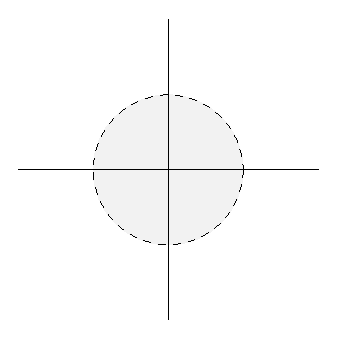
\includegraphics{Bab111}
      \end{center}
      \caption{Bola abierta con la m\'etrica usual de $\mathbb{R}^2$}
     \end{figure}
   \end{example}
   
   \begin{example} Consideremos el espacio m�trico $(\mathbb{R}^2,\rho_2)$, donde $\rho_2$ es la metrica definida en el Ejemplo~\ref{metricas en Rn}. Entonces, la bola con centro en $\bar 0=(0,0)$ y radio 1, es el conjunto dado por
     \begin{equation*}
      B(\bar 0,1)=\{(x,y)\in\mathbb{R}^2\mid |x|+|y|<1\}.
     \end{equation*}
     \begin{figure}[h!]
      \begin{center}
       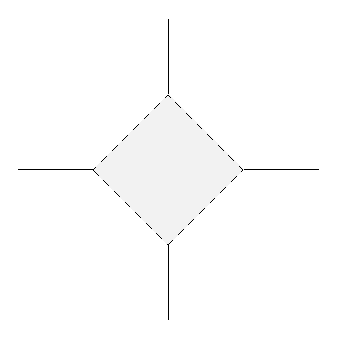
\includegraphics{Bab112}
      \end{center}
      \caption{Bola abierta con la m\'etrica citadina de $\mathbb{R}^2$}
     \end{figure}
   \end{example}
   
   \begin{example} Consideremos el espacio m�trico $(\mathbb{R}^2,\rho_3)$, con $\rho_3$ la m�trica definida en el Ejemplo~\ref{metricas en Rn}.   Entonces, la bola abierta con centro en $\bar 0=(0,0) $ y radio 1, es el conjunto 
     \begin{equation*}
      B(\bar 0,1)=\{(x,y)\in\mathbb{R}^2 \mid \max\{|x|,|y|\}\leq 1\}.
     \end{equation*}

     \begin{figure}[h!]
      \begin{center}
      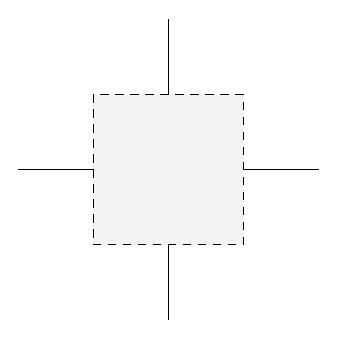
\includegraphics{Bab113}
      \end{center}
      \caption{Bola abierta con la m\'etrica del supremo de $\mathbb{R}^2$}
     \end{figure}
   \end{example}

  
  

  
  \begin{example}\label{bola discreta} Sean $(X,d)$ es un espacio  m{\'e}trico discreto, $x\in X$  y $r>0$. Entonces, si $r< 1$, 
     
    \begin{equation*}
     B(x,r)=\{x\}.
    \end{equation*}
Por otro lado, si $r\geq 1$, entonces
$$B(x,r)=X.$$

\end{example}



 
A continuaci�n, introduciremos la noci�n central para el estudio de la topolog�a: 
los conjuntos abiertos de un espacio m�trico.

 \begin{definition}
  Sean $(X,d)$ un espacio m{\'e}trico,  $A$ un subconjunto de $X$ y $x\in A$. Se dice que $x$ es \textbf{punto interior de} $A$, si existe $r>0$ tal que $B(x,r)\subset A$. El conjunto de todos los puntos interiores de $A$ se denota por $Int~A$. Es evidente que $Int~A\subset A$ para todo subconjunto $A$ de $X$.
     \smallskip
     
 Diremos que $A$ es un \textbf{conjunto abierto} en $X$ si para cada $x\in A$, $x$
         es \textbf{punto interior} de $A$. En otras palabras, $A$ es abierto si $A=Int~A$. Por otro lado, diremos que
        $A$ es un \textbf{conjunto cerrado} en $X$ si $X\setminus A$ es abierto.
   
 \end{definition}
 \begin{proposition}
  Sea $(X,d)$ un espacio m{\'e}trico. Entonces para todo $x\in X$ y $r>0$, la bola abierta
  $B(x,r)$ es un conjunto abierto en $X$.
 \end{proposition}
 \begin{proof}
  Sea $y\in B(x,r)$.  Definamos $r'$ por  $$r'=r-d(y,x).$$ Como $d(y,x)<r$, es claro que $r'>0$. 
  Consideremos $z\in B(y,r')$. Entonces $d(z,y)<r'$, y por tanto
  
    $$d(z,x)  \leq d(z,y)+d(y,x)<r'+d(y,x)=r-d(y,x)+d(y,x)=r$$

  As�, podemos concluir que $z\in B(x,r)$, de donde $B(y,r')\subset B(x,r)$. De este modo, tenemos que $y$ es punto interior de $B(x,r)$ y por lo tanto $B(x,r)$ es abierto en $X$.
 \end{proof}

 \begin{theorem}\label{espmetrico=topologico}
  Sea $(X,d)$ un espacio m{\'e}trico, entonces
  \begin{enumerate}
   \item $X,\emptyset$ son conjuntos abiertos.
   \item Si $\{U_\alpha\}_{ \alpha \in \mathcal{A}}$ es una familia arbitraria
de conjuntos abiertos en $X$,
    entonces $\bigcup\limits_{\alpha\in \mathcal{A}}U_\alpha$ es un conjunto abierto en $X$.
   \item Si $U,V\subset X$ son conjuntos abiertos en $X$, entonces $U\cap V$ es un conjunto abierto en $X$.
  \end{enumerate}
 \end{theorem}
 \begin{proof}
  \begin{enumerate}
   \item Claramente $X$ es abierto, ya que para cualesquiera $x\in X$ y $r>0$,
         $B(x,r) \subset X$, por lo que todo punto en $X$ es punto interior.
     Por otro lado,  $\emptyset$ es abierto por vacuidad.

   
  \item 
  Sea $\{U\}_{\alpha\in \mathcal A}$ una familia  arbitraria de abiertos, entonces para toda  $x \in\bigcup\limits_{\alpha\in \mathcal A}
  U_\alpha$ existe $\alpha_0$ tal que $x \in U_{\alpha_0}$. Como $U_{\alpha_0}$ es abierto en $X$,  existe $r>0$ tal que
    $B(x,r)\subset U_{\alpha_0}$, por lo tanto $B(x,r)\subset  \bigcup\limits_{\alpha\in \mathcal A}
    U_\alpha$, implicando que $x$ es punto interior de $\bigcup\limits_{\alpha\in \mathcal A} U_\alpha$. As� $ \bigcup\limits_{\alpha\in A}
    U_\alpha$ est� constitu�do en su totalidad de puntos interiores, y por tanto es un conjunto abierto de $X$.
  \item   Sean $U$ y $V$ abiertos y $x\in U\cap V$. Como
    $x\in U$,  existe $r_1>0$ tal que $B(x,r_1)\subset U$. An�logamente, como
     $x\in V$,  existe $r_2>0$ tal que $B(x,r_2)\subset V$.
    Sea $r=\min\{ r_1,r_2\}$, entonces $B(x,r)\subset U$ y $B(x,r)\subset V$, por lo que $B(x,r)\subset U\cap
    V$. As�, $x$ es punto interior de  $U\cap V$, y por tanto este conjunto  es abierto.
  \end{enumerate}
 \end{proof}
 \begin{corollary} Si $X$ es un espacio m�trico entonces $X$ y $\emptyset$ son subconjuntos abiertos y cerrados.
 \end{corollary}
 
 \begin{corollary}\label{interseccion abiertos}
  Si $U_1,\dots,U_n\subset X$ son subconjuntos abiertos de un espacio m�trico $X$, entonces
  $\bigcap\limits_{i=1}^{n}U_i$ es un subconjunto abierto en $X$.
 \end{corollary}
 
  Como se vi� en el corolario~\ref{interseccion abiertos}, la intersecci�n  
 finita de conjuntos abiertos es abierta. Sin embargo, la intersecci�n infinita de abiertos, no 
 necesariamente es abierta, como veremos en el siguiente ejemplo.

\begin{example} Sean $\mathbb{R}$ la recta real, $U_n=(\frac{-1}{n},\frac{1}{n})$ y $V_n=(n,\infty)$. Para todo $n\in\mathbb{N}$,  $U_n$ y $V_n$ son subconjuntos abiertos de $\mathbb{R}$. Por un lado $\bigcap\limits_{n=1}^\infty V_n=\emptyset$ que es
     abierto en ${{\mathbb R}}$.
Sin embargo $\bigcap\limits_{n\in\mathbb{N}}U_n=\{0\}$, el cual no es un conjunto abierto de $\mathbb{R}$. 
\end{example}

\begin{example}
Si $X$ es un espacio m�trico discreto, entonces cualquier subconjunto $U$ de $X$ es abierto en $X$.
\end{example}

 
  
   
  

  
 

\section{Subespacios M{\'e}tricos}
Es f�cil ver que para cualquier subconjunto $A$ de un espacio m�trico $(X,d)$, la restricci�n de la m�trica $d$ al subconjunto $A$ define una m�trica en $A$. As� llegamos a la siguiente definici�n.

 \begin{definition}
  Sean $(X,d)$ un espacio m{\'e}trico no vac�o, $A\subset X$ y  $d|_{A\times A}:A\times A\to \mathbb{R}$ la restricci�n de la m�trica $d$ al conjunto $A$. Entonces
   la pareja $(A,d|_{A\times A})$ recibe el nombre de \textbf{subespacio m{\'e}trico} de
  $(X,d)$.
 \end{definition}
 
 Es claro que todo subespacio m�trico es a su vez un espacio m�trico.
 
 \begin{example}[Ejemplos] Sea $(\mathbb{R}^n,\rho_1)$ como en el Ejemplo~\ref{metricas en Rn}. Los siguientes son algunos subespacios importantes.
 \begin{enumerate}
 \item La bola unitaria definida por
 $$\mathbb{B}^n=\{(x_1,\dots,x_n)\mid x_1^2+\dots +x_n^2<1\}.$$
 \item La esfera de dimensi�n $n-1$, dada por $$\mathbb{S}^{n-1}=\{(x_1,\dots,x_n)\in\mathbb{R}^n\mid~x_1^2+\dots+x_n^2=1\}.$$
 \item El cubo unitario dado por
 $$I^n=\{x_1,\dots,x_n)\in\mathbb{R}^n\mid 0\leq x_i\leq 1~
     i=1,\dots,n\}.$$
 \end{enumerate}
 \end{example}


 \section{Producto de Espacios M{\'e}tricos}


 \begin{proposition}
 Sea $\{(X_i,d_i)\}$  una colecci�n finita de espacios m�tricos. Definamos  $$ X=\prod_{i=1}^{n} X_i=\{(x_1,\dots,x_n)\mid x_i\in X_i,~ i=1,\dots,n
   \}.$$ 
  La funci�n  $d:X\times X\to\mathbb{R}$ dada por
  \begin{equation}
    d(\bar x,\bar y)=
    \sqrt{d_1^2(x_1,y_1)+\dots+d_n^2(x_n,y_n)}\notag.
  \end{equation}
  es una m�trica en $X$, por lo que  $(X,d)$ es un espacio m{\'e}trico
 \end{proposition}
La demostraci�n es an�loga a la del Ejemplo~\ref{metricas en Rn}.
\smallskip
 El espacio $(X,d)$ de la proposici�n anterior se  llama \textbf{producto 
 de espacios m{\'e}tricos}. Hay otras m�tricas que se les suele dar al espacio $X$. Algunas de las m�s comunes son las siguientes
 \begin{enumerate}
 \item $\hat d:X\times X\to\mathbb{R}$ dada por $$d(x,y)=\sum\limits_{i=1}^nd_i(x_i,y_i).$$
 \item $\tilde d:X\times X\to \mathbb{R}$ dada por
 $$d(x,y)=\max\{d_i(x_i,y_i)\}_{i=1,\dots,n}.$$
 \end{enumerate}
 
 
 \section{Continuidad}

Uno de los aspectos que m�s va a llamar nuestro inter�s es la noci�n de continuidad de una funci�n entre
dos espacios. El estudio de estas funciones es de suma importancia para
esta materia.

 \begin{definition}
  Sea $f:(X,d)\to(Y,\rho)$ una funci\'on entre dos espacios m�tricos.
 Se dice que  $f$ es continua en el punto  $x_0\in X$, si para
 todo $\varepsilon>0$ existe $\delta>0$ tal que
  $\rho(f(x),f(x_0))<\varepsilon$ siempre que $d(x,x_0)<\delta\notag.$
\smallskip
Diremos que $f$ es continua en $X$, si es continua en cualquier punto $x_0\in X$.

 \end{definition}
 
En otras palabras, diremos que una funci�n $f:(X,d)\to (Y,\rho)$  entre dos espacios m�tricos  es continua si para toda $x\in X$ y para toda $\varepsilon>0$, existe $\delta>0$, tal que $f(B(x,\delta))\subset B(f(x),\varepsilon)$.
 
Cuando los espacios $(X,d)$ y $(Y,\rho)$ coinciden con la recta real, entonces la definici�n anterior coincide con la definici�n usual de continuidad que se estudia en los cursos de c�lculo.

Es importante observar que dependiendo de las m�tricas $d$ y $\rho$ una misma funci�n puede ser continua o no. Por ejemplo, si consideramos los espacios $(\mathbb R,d)$ y 
$(\mathbb R, \rho)$, donde $d$ denota la m�trica discreta y $\rho$ la m�trica usual, entonces la funci�n identidad $Id:(\mathbb R,d)\to (\mathbb R,\rho)$ es continua,en tanto que la misma funci�n $Id:(\mathbb R,\rho)\to(\mathbb R, d) $ no lo es. 


 
 

 \begin{theorem}
  Sean $(X,d)$ y $(Y,\rho)$ dos espacios m{\'e}tricos y $f:X\to Y$ una funci�n. Entonces  los siguientes enunciados son equivalentes:
  \begin{enumerate}
  \item $f$ es continua.
  \item Para toda $y\in Y$ y para toda $\varepsilon>0$, $f^{-1}(B(y,\varepsilon))$ es abierto en $X$.
   \item Para cualquier abierto $U\subset Y$, $f^{-1}(U)$ es abierto en $X$. 
  \end{enumerate}
\end{theorem}
\begin{proof}\,\hfill \\
   

$(1\Rightarrow 2).$ Sea $y\in Y$ y $\varepsilon >0$. 
Consideremos 
     $z\in f^{-1}(B(y,\varepsilon))$, entonces
 $f(z)\in B(y,\varepsilon)$. Como $B(y,\varepsilon)$ es un 
conjunto abierto, existe $\eta>0$ tal que
    $B(f(z),\eta)\subset B(y,\varepsilon)$. Aplicando
 la continuidad de $f$ podemos encontrar 
    $\delta>0$,  tal que  $f(B(z,\delta))\subset B(f(z),\eta)$.
 As�, podemos concluir que   $B(z,\delta)\subset
    f^{-1}(B(f(z),\eta))\subset f^{-1}(B(y,\varepsilon))$, y por 
    tanto $f^{-1}(B(y,\varepsilon))$ es abierto en $X$.
  
\smallskip
$(2\Rightarrow 3)$.   Sea $U$ abierto en $Y$ y  $z\in f^{-1}(U)$. Demostraremos que $z$ es punto interior de $f^{-1}(U)$.  Notemos que  $f(z)\in U$ y por ser $U$ abierto 
    existe $\varepsilon>0$ tal que $B(f(z),\varepsilon)\subset
    U$.
     Por hip�tesis
 $f^{-1}(B(f(z),\eta))$ es abierto en $X$, entonces, existe $\delta>0$ 
tal que $$B(z,\delta)\subset f^{-1}(B(f(z),\varepsilon)).$$ Pero $f^{-1}(B(f(z),\varepsilon))$ est� contenido en  $f^{-1}(U)$, por lo que $B(z,\delta)\subset f^{-1}(U)$,  y por lo tanto $z$ es punto interior de $f^{-1}(U)$.
  

\smallskip
$(3\Rightarrow 1).$ 
    Sean $x_0 \in X$, y $\varepsilon>0$. Entonces $B(f(x_0),\varepsilon)$ es un abierto en $Y$ y por
    hip�tesis $f^{-1}(B(f(x_0),\varepsilon))$ es abierto en $X$.
     Como $x_0$ pertenece a $ f^{-1}(B(f(x_0),\varepsilon))$, existe $\delta>0$ tal que
$$B(x_0,\delta)\subset
    f^{-1}(B(f(x_0),\varepsilon)).$$ As�, $f(B(x_0,\delta))\subset B(f(x_o),\varepsilon)$, por lo que $f$ es
    continua.
  
 \end{proof}
\section{Convergencia de suceciones}

 \begin{definition}
  Sean $(X,d)$ un espacio m{\'e}trico y $(x_n)_{n\in\mathbb{N}}$ una
  sucesi{\'o}n en $X$. Se dice que $(x_n)_{n\in\mathbb{N}}$ \textbf{converge} al punto $x$, si
  para cada $\varepsilon > 0$ existe  $n_0\in\mathbb{N}$, tal que 
   $d(x_n,x)< \varepsilon$ para todo $n \geq n_0$. 
 \end{definition}
 En la literatura la convergencia de una suseci�n $(x_n)_{n\in\mathbb{N}}$ a un punto $x$, se suele denotar por $\lim\limits_{n\to\infty}x_n=x$ o por $x_n\to x$.
 
 
 \begin{proposition}
  Sea $(X,d)$ un espacio m{\'e}trico y $(x_n)_{n\in\mathbb{N}}$ una sucesi{\'o}n en $X$.
  Entonces, $x_n \rightarrow x$ si y s�lo si $d(x_n,x) \rightarrow 0$.
 \end{proposition}
 La demostraci\'on es inmediata.
 
 En los espacios m�tricos discretos, las sucesiones convergentes tienen una forma muy particular como veremos en el siguiente ejemplo.
    \begin{example}
    Sea $(X,d)$ un espacio  m�trico discreto. 
Si $(x_n)_{n\in\mathbb{N}}$ es una sucesi�n en $X$ que converge a un punto $x$, entonces existe $n_0\in\mathbb{N}$, tal que para toda $n\geq n_0$, $x_n=x$. 

En efecto, si $\varepsilon < 1$, entonces existe $n_0\in\mathbb{N}$ tal que para todo $n\geq n_0$, $x_n\in B(x,\varepsilon )$. Pero por el Ejemplo~\ref{bola discreta}, $B(x,\varepsilon)=\{x\}$, por lo que
    $x_n= x$, para todo $n\geq n_0$.
    
    \end{example}
   
\begin{proposition} Sea $(X,d)$ un espacio m�trico. Entonces toda sucesi�n convergente tiene un s�lo l�mite.
\end{proposition}

\begin{proof}
Sea $(x_n)_{n\in\mathbb{N}}$ una sucesi�n en $X$. Si $x$ y $y$ son dos puntos en $X$ tales que $\lim\limits_{n\to\infty}x_n=x$ y $\lim\limits_{n\to\infty}x_n=y$.
Supongamos que $x\neq y$. Entonces $d(x,y)>0$, por lo que $\varepsilon=\frac{d(x,y)}{2}>0$. Adem�s, es claro que $B(x,\varepsilon)\cap B(y,\varepsilon)=\emptyset$. 

Como $(x_n)$ converge a $x$, existe $n_1$ tal que si $n\geq n_1$, entonces $x_n\in B(x,\varepsilon)$. An�logamente, existe $n_2$ tal que si $n\geq n_2$, entonces $x_n\in B(y,\varepsilon)$. Sea $n_0=\max\{n_1,n_2\}$, entonces, si $n\geq n_0$, $x_n\in B(x,\varepsilon)\cap B(y,\varepsilon)$ lo cual es una evidente contradicci�n. Por lo tanto $x=y$.
\end{proof}
Las sucesiones juegan un papel determinante en la continuidad de las funciones entre espacios m�tricos. El siguiente teorema nos dice porqu�.
\begin{theorem}
  Sean $(X,d)$ y $(Y,\rho)$ dos espacios m\'etricos.  Una funci�n $f:X\to Y$ es continua en $x_0\in X$ si y s�lo si, para cualquier sucesi�n $(x_n)_{n\in\mathbb{N}}$ que converja a $x_0$ la sucesi�n $(f(x_n))_{n\in\mathbb{N}}$ converge a $f(x_0)$. 
 \end{theorem}
 
 \begin{proof}
 Primero demostraremos la parte \textit{si}. Sea $(x_n)_{n\in\mathbb{N}}$ una sucesi�n en $X$ convergente al punto $x_0\in X$. Por la continuidad de $f$, dado $\varepsilon>0$ existe 
$\delta>0$ tal que si $x \in B(x_0, \delta)$, entonces 
   $f(x) \in B(f(x_0), \varepsilon)$. 
Como
   $x_n$ converge a $ x_0$, podemos encontrar  $n_0 \in \mathbb{N}$, tal que   $x_n \in B(x_0, \delta)$
   para todo $n \geq n_0$. Luego $f(x_n) \in B(f(x_0), \varepsilon)$ para todo $n \geq n_0$, lo cual demuestra que $(f(x_n))_{n\in\mathbb{N}}$ converge a $f(x_0)$.
   \smallskip
   
   Ahora demostraremos la parte \textit{s�lo si}. Demostraremos que $f$ es continua por contradicci�n. Supongamos que existe $\varepsilon_0>0$, tal que para toda $\delta>0$, existe $x\in B(x_0,\delta)$ tal que $x\notin B(f(x_0),\varepsilon_0)$.
   Construiremos una sucesi�n $(x_n)_{n\in\mathbb{N}}$ en $X$ tal que $x_n\to x_0$, pero de manera que la sucesi�n $(f(x_n))_{n\in\mathbb{N}}$ no converja a  $f(x_0)$.

 Para $\delta_1=1$, escojamos $x_1\in B(x_0,1)$ tal que $f(x_1)\notin B(f(x_0),\varepsilon_0)$. An�logamente, para $\delta_2=\frac{1}{2}$, escojamos $x_2\in B(x_0,\frac{1}{2})$ tal que $f(x_n)\notin B(f(x_0),\varepsilon_0)$. As�, para $\delta_n=\frac{1}{n}$ podemos escoger $x_n\in B(x_0,\frac{1}{n})$ tal que $f(x_n)\notin B(f(x_0),\frac{1}{n})$. Claramente, la sucesi�n $(x_n)_{n\in\mathbb{N}}$ converge a $x_0$. Pero la construcci�n nos grantiza que $(f(x_n))_{n\in\mathbb{N}}$ no converge a $f(x_0)$, contradiciendo la hip�tesis. 
 Por lo tanto, $f$ es continua en $x_0$, como se quer�a demostrar.

 \end{proof}

 
 
 \section{Espacios normados}
 A continuaci�n introduciremos un tipo de espacios m�tricos que por sus car�cteristicas geom�tricas merecen ser tratados por separado.
 \begin{definition}\label{def norma}
  Sea $X$ un espacio lineal (sobre $\mathbb{R}$ {\'o} $\mathbb{C}$).
  Una \textbf{norma} es  una funci{\'o}n $\parallel \cdot \parallel :X\to\mathbb{R}$ la cual satisface los siguientes axiomas:
  \begin{enumerate}
   \item  $\|x\|\geq 0$. Adem�s $\|x\|=0$ si y s�lo si $x=0$,
   \item  $\|\lambda x\|=|\lambda| \|x\|$,
   \item  $\|x+y\|\leq\|x\|+\|y\|$,
  \end{enumerate}
  donde $x,y\in X$ y $\lambda\in\mathbb{K}=\mathbb{R}$ � $\mathbb{C}$. El par $(X,\|\cdot\|)$ recibe el nombre de \textbf{espacio lineal normado}.  
 \end{definition}
 
 
 \begin{proposition}
 Sea $(X, \|\cdot\|)$  un espacio lineal normado. Definamos la funci�n 
$d:X\times X\to\mathbb R$, por
 $d(x,y)=\|x-y\|$. Entonces, 
  $d$ es una m{\'e}trica en $X$.
 \end{proposition}
 \begin{proof}
  Se sigue de la definici�n de norma que siempre $d(x,y)\geq 0$ y $d(x,y)=0$ si y s�lo si $x-y=0$, lo cual sucede siempre y cuando $x=y$.
Por otro lado, $$d(x,y)=|x-y\|=\|-(y-x)\|=|-1|\|y-x\|=\|y-x\|=d(y,x).$$ 
 
 Para completar la demostraci�n, s�lo resta verificar la desigualdad del tri�ngulo.
  Para ello tomemos tres puntos $x,y,z\in X$.  Entonces
  \begin{equation*}
    d(x,z)=\|x-z\|
                =\|x-y+y-z\|                
                \leq \|x-y\|+\|y-z\|\\
                =d(x,y)+d(y,z).
  \end{equation*}
As�, podemos concluir que $d$ es una m�trica.
 \end{proof}

Se sigue de la proposici�n anterior que todos los espacios normados son a su vez espacios m�tricos.
Veamos algunos ejemplos.


 
 \begin{example} Sea $X$ un conjunto no vac�o. Consideremos el conjunto de todas las funciones  acotadas de $X$ en $\mathbb{R}$, denotado por $B(X)$.
    
    $B(X)$ es un espacio lineal, 
donde la suma est\'a definida por $(f+g)(x)=f(x)+g(x)$; el producto
    por escalares por $(\lambda f)(x)=\lambda f(x)$; y,  la funci\'on cero
    como $\theta(x)=0$. La funci�n $\|\cdot\|:B(X)\to\mathbb{R}$ dada por  $\|f\|=\sup\{|f(x)||x\in X\}$ define una norma en $B(X)$.  Esta norma recibe el nombre de 
    \textbf{norma uniforme} o \textbf{norma del supremo}.

   
   \begin{proof}
      \begin{enumerate}
        \item Es evidente que para cualquier $f\in B(X)$, $\|f\|\geq 0$. Por otro lado, como $\sup\limits_{x\in X}\{ |f(x)|\}\geq~|f(x)|$ para cualquier $x\in
        X$, es claro que $\|f\|=0$ si y s�lo si $f(x)=0$ para toda $x\in X$.

      \item Sea $f\in B(X)$ y $\lambda\in\mathbb{R}$. Entonces, 
        \begin{equation*}
          \|\lambda f\|=\sup\limits_{x\in X}|\lambda f(x)|=\sup\limits_{x\in X}|\lambda||f(x)|=
          |\lambda|\sup\limits_{x\in X}|f(x)|=|\lambda|\|f\|.
        \end{equation*}
      \item Sean $f,g\in B(X)$. Entonces
        \begin{equation*}
        \|f+g\|=\sup\limits_{x\in X}|f(x)+g(x)|
        \leq\sup\limits_{x\in X}|f(x)|+\sup\limits_{x\in X}|g(x)|=
          \|f\|+\|g\|,
        \end{equation*}
      \end{enumerate}
      lo cual muestra que $\|\cdot\|$ es una norma en $B(X)$.
    \end{proof}
\end{example}       
  \begin{example}\label{espaciodehilbert}
Denotemos por $\ell_2$ el conjunto dado por
   \begin{equation*}
    \ell_2=\left\{x=(x_1,x_2,\dots)\left|~
        x_i\in \mathbb{R},~\sum_{i=1}^\infty|x_i|^2<\infty\right.
    \right\}.
   \end{equation*}
   $\ell_2$ es un espacio lineal, d�nde  la suma est� definida por $x+y=(x_1+y_1,x_2+y_2,\dots)$; el producto por escalares por $\lambda x=(\lambda x_1,\lambda x_2,\dots);$ y el vector cero es el punto $(0,0,\dots)$.

Se define en $\ell_2$ la funci�n $\|\cdot\|:\ell_2\to\mathbb{R}$, de la siguiente manera:  
    $$\|x\|=\sqrt{\sum_{i=1}^\infty|x_i|^2}.$$
El espacio $(\ell_2,\|\cdot\|)$ es un espacio normado
  conocido como \textbf{espacio de Hilbert}.

  \begin{proof}
   Primero veamos que $\ell_2$ es cerrado bajo la suma y la m�ltiplicaci�n por escalares. En efecto, si $x=(x_1,x_2,\dots)$, y $y=(y_1,y_2\dots)$ son dos puntos arbitrarios de $ \ell_2$, 
   \begin{equation*}
    \sum_{i=1}^{\infty}\left|x_i + y_i\right|^2 = \sum_{i=1}^{\infty}(\left|x_i\right|^2 +
     2\left|x_i\right|\left|y_i\right| + \left|y_i\right|^2)
     =\sum_{i=1}^{\infty}\left|x_i\right|^2 +
     2\sum_{i=1}^{\infty}\left|x_i\right|\left|y_i\right| +
     \sum_{i=1}^{\infty}\left|x_i\right|^2.
   \end{equation*}
   
 Pero el primer y  el \'ultimo  sumando  son  series convergentes, por lo que para demostrar la convergencia de $\sum\limits_{i=1}^{\infty}\left|x_i + y_i\right|^2$ s\'olo faltar�a demostrar  la convergencia
  de la serie $\sum\limits_{i=1}^{\infty}|x_i||y_i|$. Aplicando  la 
   desigualdad de Cauchy-Schwarz, tenemos que
    $$\sum_{i=1}^n|x_i||y_i|\leq\sqrt{\Big{(}\sum_{i=1}^n|x_i|^2\Big{)}\Big{(}\sum_{i=1}^n|y_i|^2\Big{)}}.$$
    Tomando el l�mite cuando $n$ tiente a infinito, tenemos que 
     \begin{equation}\label{d:c s}  \sum_{i=1}^{\infty}\left|x_i\right|\left|y_i\right| \leq
      \sqrt{\Big{(}\sum_{i=1}^{\infty}\left|x_i\right|^2 \Big{)}\Big{(}\sum_{i=1}^{\infty}\left|y_i\right|^2\Big{)}}.
\end{equation}

   Como  las series
   $\sqrt{\sum_{i=1}^{\infty}\left|x_i\right|^2}$ y $\sqrt{\sum_{i=1}^{\infty}\left|y_i\right|^2}$
   convergen, el producto 
   $$\Big{(}\sum_{i=1}^{\infty}\left|x_i\right|^2 \Big{)}\Big{(}\sum_{i=1}^{\infty}\left|y_i\right|^2\Big{)}<\infty.$$  Luego
   $$ \sum_{i=1}^{\infty}\left|x_i\right|\left|y_i\right| \leq \infty ,$$
   como se quer�a demostrar.
   
   Por otro lado, 
  si $x\in\ell_2$ y $\lambda \in\mathbb{R}$,  se tiene que:
    \begin{equation*}
      \sum_{i=1}^\infty|\lambda
      x_i|^2=\sum_{i=1}^\infty|\lambda|^2|x_i|^2 =
      |\lambda|^2\sum_{i=1}^\infty|x_i|^2<\infty,
    \end{equation*}
    lo cual implica que $\lambda
    x\in\ell_2$.
    Por \'ultimo, verificaremos que la funci�n $\|\cdot\|$ es una norma. Es claro que $\|\cdot\|$ satisface los axiomas $1$ y $2$ de la definici�n~\ref{def norma}. 

   Como hemos visto anteriormente $\|x+y\|^2=\|x\|^2+\|y\|^2+2\sum\limits_{i=1}^{\infty}|x_i||y_i|$. Observemos que de la desigualdad~(\ref{d:c s}), se sigue directamente que 
   $$\sum\limits_{i=1}^{\infty}|x_i||y_i|\leq \|x\|\|y\|,$$
   por lo que
   $$\|x+y\|^2\leq\|x\|^2+\|y\|^2+2\|x\|\|y\|=(\|x\|+\|y\|)^2.$$
   De donde podemos concluir que $\|x+y\|\leq\|x\|+\|y\|$.
  \end{proof}
\end{example}
\section{Ejercicios del cap\'\i tulo}
 \begin{enumerate}[1.]
  
  \item Sea $X=\{1,2,3\}$. Queremos construir una m\'etrica para $X$,
   que satisfaga $d(1,2)=2$ y $d(1,3)=3$ �Cu\'al debe ser el valor de
   $d(2,3)$ para que $d$ sea m\'etrica?
  \item Sea $X\neq\emptyset$. Prueba que si $d(x,y)$ satisface que
   $d(x,y)\geq 0$, $d(x,y)=0$
   si y s�lo si $x=y$ y la desigualdad del tri\'angulo, entonces
   $d'(x,y)=d(x,y)+d(y,x)$ es una m\'etrica para $X$.
  \item ?` Cu\'ales de las siguientes son m\'etricas para $\mathbb{R}$?
   \begin{enumerate}
    \item $d(x,y)=(x-y)^2,$
    \item $d(x,y)=\sqrt{|x-y|},$
    \item $d(x,y)=|x^2-y^2|,$
    \item $d(x,y)=||x|-|y||.$
   \end{enumerate}
  
  
\item Sea $X$ el conjunto formado por las casillas de un tablero de ajedrez como el que se ilustra a continuaci�n.

 \begin{figure}[h!]
      \begin{center}
      \includegraphics*[scale=0.2]{tablero}
      \end{center}
   \end{figure}
 Considermos el caballo (C), la Reina (D), el rey (R) y la torre (T). Para cada una de estas piezas definamos las siguientes funciones de $X\times X$ en $\mathbb{R}$:
\begin{enumerate}  
\item $d_C(x, y)=$ m�nimo n�mero de movimientos que  necesita un caballo para ir de la casilla $x$ a la casilla $y$, 
\item $d_D(x,y)=$ m�nimo n�mero de movimientos que  necesita la Reina para ir de la casilla $x$ a la casilla $y$,
\item $d_R(x,y)=$ m�nimo n�mero de movimientos que  necesita un Rey para ir de la casilla $x$ a la casilla $y$,
\item $d_T(x,y)=$ m�nimo n�mero de movimientos que  necesita una torre para ir de la casilla $x$ a la casilla $y$.
  \end{enumerate}
  Por ejemplo, $d_C(B2,G6)=3$, mientras que $d_D(B2,G6)=2$.
  Demuestra que cada una de estas funciones define una m�trica en $X$ �Porqu� el alfil no puede definir una m�trica en $X$?
  Para cada una de las m�tricas describe c�mo ser�an las bolas abiertas.
  \item Da un ejemplo de un espacio m�trico  $X$, en el cual existan puntos $x$ y $y$, tales que $B(x,r)\subsetneqq B(y,q)$ con $r>q$.
  \item Define una m�trica $d$ en $\mathbb{R}^2$ tal que la bola unitaria coincida con el interior de la elipse dada por $\frac{x^2}{a^2}+\frac{y^2}{b^2}=1$; es decir, $B((0,0),1)=\{(x,y)\in\mathbb{R}^2|~\frac{x^2}{a^2}+\frac{y^2}{b^2}<1\}$, con $a$ y $b$ n�meros reales positivos.
  \item Sean $d_X$ y $d_Y$ m\'etricas para los espacios $X$ y $Y$
   respectivamente. Menciona al menos dos m\'etricas para el producto
   $X\times Y$.
  \item Sean $X=[0,1)$ y $\rho:X\times X\to \mathbb{R}$ dada por 
  $$\rho(x,y)=\min \{|x-y|,1-|x-y|\}.$$
  Demuestra que $\rho$ es una m�trica en $X$. Interpreta geom�tricamente.
  \item Considera el espacio m�trico $(X,\rho)$ del ejercicio anterior. Sea $f:X\to\mathbb{R}$ dada por $f(x)=x$ �Es continua esta funci�n?
  \item Demuestra que si $(X,d)$ es un espacio m�trico discreto, y $Y$ es un espacio m�trico arbitrario, entonces cualquier funci�n $f:X\to Y$ es continua.
   \end{enumerate}
 
\end{document}

%\documentclass[12pt]{amsbook}
\usepackage{latexsym,amssymb,amsmath}
\usepackage[spanish]{babel}
\usepackage{enumerate}
\usepackage{graphicx}
\usepackage[all]{xy}
%\usepackage{theorem}
%Nuevo
%\usepackage{makeidx}
\usepackage{color,soul}
%Nuevo
\usepackage[latin1]{inputenc}
\newtheoremstyle{Normal}{5pt}{5pt}{\itshape}{}{\bfseries}{.}{.5em}{}
\theoremstyle{Normal}
\newcounter{Mio}
\newtheorem{definition}{Definici\'on}[section]
\newtheorem{proposition}[definition]{Proposici\'on}
\newtheorem{theorem}[definition]{Teorema}
\newtheorem{corollary}[definition]{Corolario}
\newtheorem{nota}[definition]{Nota}
\newtheorem{lemma}[definition]{Lema}
\newtheorem{property}[definition]{Propiedad}
\newtheoremstyle{Ejemplos}{10pt}{10pt}{\slshape}{}{\bfseries}{.}{.5em}{
\nopagebreak\hskip -.5em
\hrulefill\rule{\textwidth}{1pt}\rule{1em}{1pt}\rule[-10pt]{1pt}{11pt}\\[-7pt]\nopagebreak#1 #2#3}
\theoremstyle{Ejemplos}
%\newtheorem{example}[definition]{Ejemplo}
%\newtheorem{example}{
%  \textbf{
%    \hskip-45pt\vrule\rule[-10pt]{3pt}{10pt}\hrulefill\\
%    Ejemplo}
%}
\newenvironment{example}[1][Ejemplo]{\par
\nopagebreak\noindent\rule{\textwidth}{1pt}\rule{1em}{1pt}\rule[-8pt]{1pt}{9pt}\\[-6pt]\nopagebreak
{\bfseries #1 \addtocounter{Mio}{1}\arabic{Mio}. } }
{\hfill\\[-6pt]\nopagebreak\rule{\textwidth}{1pt}\rule{1em}{1pt}\rule[0pt]{1pt}{8pt}\\[.5em]\nopagebreak}


\numberwithin{section}{chapter}
\textwidth=390pt
\addtolength{\hoffset}{-1.5cm}
\definecolor{lightblue}{rgb}{.70,.70,1}
\sethlcolor{lightblue}
\makeindex
\begin{document}
\chapter{Espacios Topol\'{o}gicos}
En este cap\'{\i}tulo introduciremos las nociones b\'{a}sicas de la
topolog\'{\i}a general. La idea principal es llevar el concepto de
conjunto abierto en un espacio m\'{e}trico, introducido en el cap\'{\i}tulo anterior, a una
noci\'{o}n m\'{a}s abstracta que nos permita generalizar algunos de los
conceptos y propiedades de los espacios m\'{e}tricos a otro tipo de
estructuras matem\'{a}ticas,  a las que llamaremos {\it espacios
topol\'{o}gicos.}
\index{espacios!topol\'ogicos}

\section{Espacios Topol\'{o}gicos}

\index{topolog\'ia}
\index{conjunto!abierto}
\begin{definition}
  Sea $X$ un conjunto no vac\'{\i}o. Una colecci\'{o}n $\tau$ de subconjuntos de $X$ se llama \textbf{topolog\'{\i}a} en $X$, si se satisfacen los siguientes axiomas: 
  \begin{enumerate}
  \item El conjunto vac\'{\i}o y $X$ est\'an en $\tau$.
  \item Si $\{U_\alpha\}_{\alpha\in \mathcal{A}}$ es una familia cualquiera de elementos de $\tau$, entonces la uni\'on $\bigcup\limits_{\alpha\in \mathcal{A}}U_\alpha$ est\'a en $\tau$.
  \item Si $\{U_1, \ldots ,U_n\}$ es una familia finita de elementos de $\tau$, entonces la intersecci\'on $U_1\cap \cdots \cap U_n$ es elemento de $\tau$.
  \end{enumerate}
  Los elementos de $\tau$ reciben el nombre de conjuntos
  \textbf{abiertos} de $X$, y 
  al conjunto  $X$ junto  con la topolog\'{\i}a $\tau$ se llama
  \textbf{espacio topol\'{o}gico}.
\end{definition}

\begin{nota} 
Hay dos cosas que definen un espacio topol\'ogico: un conjunto subyacente $X$ y una familia $\tau$ de subconjuntos de $X$ que constituye una topolog\'{\i}a. Formalmente un espacio topol\'ogico es un par ordenado $(X, \tau)$. Pero por lo general, cuando no haya riesgo de confusi\'on vamos a denotar al espacio topol\'ogico $(X, \tau)$ simplemente por $X$ dejando impl\'icitamente claro que hay una topolog\'{\i}a $\tau$ en $X$. A los elementos de $X$ se les suele llamar puntos. 
\end{nota}

As\'{\i}, en un espacio topol\'ogico $X$ el conjunto vac\'{\i}o y $X$ son abiertos, la uni\'on de cualquier familia de abiertos es un conjunto abierto, y la intersecci\'on de toda familia finita de abiertos es tambi\'{e}n un conjunto abierto.

Si el lector tiene una idea sobre c\'{o}mo son los conjuntos abiertos en la recta real o en el plano, es importante que no trate de imaginar conjuntos ``abiertos t\'{\i}picos'' de esta forma en un espacio topol\'{o}gico abstracto. En general, cualquier subconjunto de un conjunto dado $X$  puede ser abierto si la topolog\'{\i}a en $X$ se elige apropiadamente.

\begin{example}[Ejemplos]\ref{ejemplos1}
\begin{enumerate}

\item Sea $(X,d)$ un espacio m\'etrico, y sea $\tau_d$ la familia de todos los subconjuntos abiertos de $X$ en el sentido de la m\'{e}trica $d$, como se vi\'{o} en el cap\'{\i}tulo anterior. Entonces $\tau_d$ es una topolog\'{\i}a en $X$, llamada la topolog\'{\i}a generada por la m\'{e}trica $d$. (Ver el teorema \ref{espmetrico=topologico}). Llamaremos \textbf{metrizable} a cualquier espacio topol\'{o}gico $(X, \tau)$ cuya topolog\'{\i}a es generada por alguna m\'{e}trica $d$. N\'{o}tese la diferencia de este concepto con el de espacio m\'{e}trico, que es un espacio dotado de una m\'{e}trica particular expl\'{\i}cita. En tanto que cada m\'{e}trica $d$ para $X$ induce una \'{u}nica topolog\'{\i}a $\tau_d$, dado un espacio metrizable $(X, \tau)$ con m\'{a}s de un punto siempre es posible hallar muchas m\'{e}tricas que generen su topolog\'{\i}a, por ejemplo si $\tau =\tau_d$, entonces tambi\'{e}n $\tau=\tau_{2d}$. 

\item Sea $X$ un conjunto no vac\'{\i}o. La colecci\'{o}n $\tau=2^X$ de todos los subconjuntos de $X$ forma una topolog\'{\i}a en $X$, llamada topolog\'{\i}a \textbf{discreta}. \index{topolog\'ia!discreta}


\item  Sea $X$ un conjunto no vac\'{\i}o. Entonces $\tau=\left\{\emptyset,X\right\}$ es una topolog\'{\i}a en $X$, llamada topolog\'{\i}a \textbf{trivial} o \textbf{antidiscreta}.
 \index{topolog\'ia!antidiscreta o trivial}


\item  Sea $X$ un conjunto no vac\'{\i}o y $A$ un subconjunto de $X$. Entonces $\tau = \{\emptyset, A, X\}$ es una topolog\'{\i}a en $X$.

\item  Sea $X$ cualquier conjunto infinito. La colecci\'{o}n $$\tau=\left\{U\subset X \mid X\setminus U \text{ es finito}\right\} \cup \{\emptyset\},$$ 
 es una topolog\'{\i}a en $X$, llamada topolog\'{\i}a \textbf{cofinita}.

\index{topolog\'ia!cofinita}
\begin{proof}\hfill
  \begin{itemize}
  \item Por definici\'{o}n $\emptyset \in \tau$. Por otro lado, $X\setminus X=\emptyset$ es finito, de donde concluimos que $X$ pertenece a $\tau$. 
  \item Sea $\{U_\alpha\}_{\alpha\in \mathcal{A}}$ una familia arbitraria de elementos de $\tau$.  Entonces $X\setminus U_\alpha$ es un subconjunto finito para cada $\alpha \in \mathcal{A}$. As\'{\i}, $$X\setminus\underset{\alpha\in \mathcal{A}}{\bigcup} U_\alpha= \underset{\alpha\in \mathcal{A}}{\bigcap}(X\setminus U_\alpha)$$ es una intersecci\'{o}n de conjuntos finitos y por tanto es finita. De este modo, tenemos que $\underset{\alpha\in \mathcal{A}}{\bigcup}U_\alpha\in\tau$. 
  \item Sean $U,V\in\tau.$ Entonces $X\setminus U$ y $X\setminus V$ son subconjuntos finitos de $X$, y por tanto su uni\'{o}n $$(X\setminus U)\cup(X\setminus V)=X\setminus(U\cap V)$$ es un subconjunto finito. Por esta raz\'{o}n podemos concluir que $U\cap V$ es un elemento de $\tau$.
  \end{itemize}
As\'{\i},  $\tau$ es una topolog\'{\i}a en $X$.
\end{proof}

\item  Sea $X$ cualquier conjunto infinito. La familia $$\tau=\left\{U\subset X~|~ X\setminus U \text{ es numerable}\right\} \cup \left\{\emptyset\right\}$$ 
  es una topolog\'{\i}a en $X$, llamada topolog\'{\i}a \textbf{conumerable}. \index{topolog\'ia!conumerable}

\item \label{espacio co-B}
Sean $X$ un conjunto no vac\'{\i}o y $B\subset X$. Entonces $$\tau=\left\{U\subset X~|~ B\subset U \right\} \cup \left\{\emptyset\right\}$$
es una topolog\'{\i}a en $X$. 

\item  Sea $X$ un conjunto no vac\'{\i}o y $B\subset X$. Entonces $$\tau=\left\{U\subset X~|~ U\cap B=\emptyset \right\} \cup \left\{X\right\}$$
es una topolog\'{\i}a en $X$. 


\item  Sea $X$ el conjunto de tres puntos $\{a,b,c\}$. Consideremos cuatro familias de subconjuntos de $X$


   $\tau_1=\{\{a\},\{a,b\},\emptyset, X\}$.

   $\tau_2=\{\{a\},\{b\},\{a,b\},\{b,c\},\emptyset,X\}$.

   $\tau_3=\{\{a,c\},\emptyset,X\}$.

   $\tau_4=\{\{a\},\{b\},\{a,b\},\{c\},\emptyset , X\}$.


  Entonces $\tau_1,\tau_2$ y $\tau_3$ son topolog\'{\i}as en $X$ pero $\tau_4$ no lo es.

\end{enumerate}
\end{example}



Los ejemplos anteriores muestran que en un mismo conjunto pueden definirse varias topolog\'{\i}as. Estas topolog\'{\i}as a veces pueden ser
comparables. As\'{\i} arribamos a la siguiente definici\'{o}n. 

\begin{definition}
    Sean $\tau_1$ y $\tau_2$ dos topolog\'{\i}as en un conjunto no vac\'{\i}o $X$. Si $\tau_{1} \subset \tau_{2}$ diremos que $\tau_1$ es
    \textbf{m\'as d\'ebil} o \textbf{m\'as gruesa} que $\tau_2$ y $\tau_2$ es \textbf{m\'as fuerte} o \textbf{m\'as fina} que $\tau_1$. 
\end{definition}\index{topolog\'ia!comparaci\'on}
\begin{example}[Ejemplos]
\begin{enumerate}
\item Sea $X$ un conjunto no vac\'{\i}o, y $\tau$ una topolog\'{\i}a para $X$. Claramente $\{\emptyset, X\}\subset \tau\subset 2^X$. Esto es, las topolog\'{\i}as trivial y discreta son respectivamente las topolog\'{\i}as m\'{a}s d\'{e}bil y m\'{a}s fuerte que se pueden definir para $X$.
\item Sea $(X,d)$ un espacio m\'{e}trico. Entonces la topolog\'{\i}a generada por la m\'{e}trica $d$ es m\'{a}s fuerte que la topolog\'{\i}a cofinita.
\end{enumerate}
\end{example}


\section{Interior y vecindades}

\begin{definition}[1]
    Sea $X$ es un espacio topol\'{o}gico
    \begin{enumerate}
    \item Para todo $x\in X$, diremos que $U$ es \textbf{vecindad} de $x$, si $U$ es un abierto en $X$ que contiene a $x$. \index{vecindad!de un punto}
    \item Si $A\subset X$. Se dice que $x$ es un \textbf{punto interior} de $A$, si existe una vecindad $U$ de $x$ tal que $U\subset A$. \index{punto!interior}
    \end{enumerate}
  \medskip
  
  El conjunto de los puntos interiores de $A$ se llama \textbf{interior} de $A$ y se denota por ${\rm{Int}}\,A$ o $\mathring{A}$.\index{interior} Claramente ${\rm{Int}}\,A\subset A$.
\end{definition}


La siguiente proposici\'{o}n nos muestra que el interior de $A$ es el subconjunto abierto m\'{a}s grande contenido en $A$. 

\begin{proposition}\label{interior=uniondeabiertos}
  Sean $X$ un espacio topol\'{o}gico y $A$ subconjunto de $X$. Entonces el interior de $A$ es la uni\'on de todos los subconjuntos abiertos de $X$ contenidos en $A$.
\end{proposition}

\begin{proof}
  Sea $x\in {\rm{Int}}\,A$. Entonces existe una vecindad $V$ de $x$, tal que $V\subset A$. As\'{\i}, $V\subset\{U~|~U\subset A,~U\text{ es abierto}\}$, lo que nos garantiza que 
    $$x\in V \subset \bigcup\{U~|~U\subset A,~U\text{ es abierto}\}\text{.}$$ 
  
Por otro lado, si $x$ es un punto de la uni\'on, existe un abierto $U$ contenido en $A$, tal que $x\in U$, por tanto $x\in {\rm{Int}}\,A$. As\'{\i} podemos concluir que ${\rm{Int}}\, A=\bigcup\{U~|~U\subset A,~U \text{ es abierto}\}$. 
\end{proof}
\begin{proposition}\label{interior=abierto} 
  Sean $X$ un espacio topol\'{o}gico y $A\subset X$. Entonces $A$ es abierto si y s\'{o}lo si $A={\rm{Int}}\,A$. 
\end{proposition}
\begin{proof}
  Supongamos que $A$ es abierto. Por esta raz\'{o}n $A\in \{U~|~U\subset A, U \text{ es abierto}\}$, luego 
  $$A\subset\bigcup\{U~|~U\subset A, ~U \text{ es abierto}\}= {\rm{Int}}\,A \text{.}$$
  
  La  contenci\'{o}n ${\rm{Int}}\,A\subset A$ se cumple siempre y por tanto $A= {\rm{Int}}\,A$. Ahora, si $A= {\rm{Int}}\,A$, por la proposici\'{o}n \ref{interior=uniondeabiertos} tenemos que $A$ es uni\'{o}n de abiertos y por consiguiente es abierto. 
\end{proof}

\begin{proposition}\label{interiorcreciente}
Sea $X$ un espacio topol\'ogico. Si $A\subset B\subset X$, entonces ${\rm{Int}}\,A\subset {\rm{Int}}\,B$.
\end{proposition}
\begin{proof}
  Sea $x\in {\rm{Int}}\,A$. Como $x\in {\rm{Int}}\,A$ entonces existe una vecindad $U$  de $x$ contenida en $A$ y como $A\subset B$, es claro que $U\subset B$
  y por lo tanto $x\in {\rm{Int}}\,B$. 
\end{proof}

\begin{theorem}\label{Teo:Propiedades interior}
  Si $X$ es un espacio topol\'{o}gico, entonces para cualesquiera dos subconjuntos $A$ y $B$ de $X$ se satisfacen los siguientes enunciados: 
  
  \begin{enumerate}
  \item ${\rm{Int}}\,X=X$.
  \item ${\rm{Int}}\,A\subset A$. 
  \item ${\rm{Int}}\,({\rm{Int}}\,A)={\rm{Int}}\,A$.
  \item ${\rm{Int}}\,(A\cap B)={\rm{Int}}\,A\cap {\rm{Int}}\,B$.
  \end{enumerate}
\end{theorem}

\begin{proof}\hfill
  \begin{enumerate}
  \item Como $X$ es un conjunto abierto, se sigue de la proposici\'on \ref{interior=abierto} que ${\rm{Int}}\,(X)=X$.
  \item Es inmediato de la definici\'on de ${\rm{Int}}\,A$.
  \item Para demostrar que ${\rm{Int}}\,({\rm{Int}}\,A)= {\rm{Int}}\,A$, simplemente notemos que ${\rm{Int}}\,A$ es abierto y apliquemos nuevamente la proposici\'on
    \ref{interior=abierto} para obtener ${\rm{Int}}\,({\rm{Int}}\,A)= {\rm{Int}}\,A$. 
  \item Como $A\cap B\subset A$ y $A\cap B\subset B$, por la proposici\'on \ref{interiorcreciente} ${\rm{Int}}\,(A\cap B)\subset {\rm{Int}}\,A$ e ${\rm{Int}}\,(A\cap B)\subset {\rm{Int}}\,B$, de donde ${\rm{Int}}\,(A\cap B)\subset {\rm{Int}}\,A \cap {\rm{Int}}\,B$. Por otro lado, notemos que ${\rm{Int}}\,A \cap  {\rm{Int}}\,B$ es un subconjunto abierto contenido en $A\cap B$. Entonces, ${\rm{Int}}\,A  \cap {\rm{Int}}\,B \subset {\rm{Int}}\,(A\cap B)$. As\'{\i} podemos concluir que ${\rm{Int}}\,(A\cap B)={\rm{Int}}\,A\cap {\rm{Int}}\,B$.     
  \end{enumerate}
\end{proof}

\begin{theorem}\label{phi=int}
  Sean $X$ un conjunto no vac\'{\i}o y $\phi:2^X\to 2^X$ una funci\'on que satisface las siguientes propiedades:
  \begin{enumerate}
  \item $\phi(X)=X$.
  \item $\phi(A)\subset A$. 
  \item $\phi(\phi(A))=\phi(A)$.
  \item $\phi(A\cap B)=\phi(A)\cap \phi(B)$.
  \end{enumerate}
  para todo par de subconjuntos $A$ y $B$ de $X$.
  
  Entonces existe una \'unica topolog\'{\i}a $\tau$ en $X$ cuyo operador interior es exactamente igual a $\phi$, es decir, $\phi(A)= {\rm{Int}}\,A$ para todo subconjunto $A$ de $X$, donde ${\rm{Int}}$ es el operador interior respecto a la topolog\'{\i}a $\tau$. 
\end{theorem}

Antes de demostrar el teorema anterior, necesitamos la siguiente
proposici\'on: 

\begin{proposition}\label{phiAphiB}
  Sea $\phi$ una funci\'on como se describe en \ref{phi=int}. Entonces
  para todo par de subconjuntos $A$ y $B$ de $X$ tales que $A\subset
  B$, se tiene que $\phi(A)\subset\phi(B)$. 
\end{proposition}
\begin{proof}
  Tenemos
  que $A=A\cap B$. Aplicando la propiedad 4, obtenemos $\phi(A)=\phi(A\cap B)=\phi(A)\cap\phi(B)$ y por lo tanto $\phi(A)\subset\phi(B)$.   
\end{proof}


\begin{proof}[Demostraci\'on del teorema \ref{phi=int}]
  Afirmamos que $\tau$, definida como:
   $$\tau=\{A\subset X \mid \phi(A)=A\} ,$$
  
es la topolog\'{\i}a buscada.
  \begin{enumerate}
  \item Por la definici\'on de $\phi$, tenemos que $X\in \tau$. Como $\phi(\emptyset)\subset\emptyset$ entonces $\phi(\emptyset)=\emptyset$ y por lo tanto $\emptyset\in \tau$.
  
  \item Sea $\{A_s\}_{s\in S}\subset \tau$. Para todo $s_0\in S$, tenemos que $A_{s_0}\subset\underset{s\in \mathcal{S}}{\bigcup} A_s$ y en consecuencia $\phi(A_{s_0})\subset\phi(\underset{s\in \mathcal{S}}{\bigcup} A_s)$. Como $A_{s_0}=\phi(A_{s_0})$, se tiene que $A_{s_0}\subset\phi(\underset{s\in \mathcal{S}}{\bigcup}
    A_s)$. De aqu\'{\i} obtenemos $\underset{s\in \mathcal{S}}{\bigcup} A_s\subset\phi(\underset{s\in \mathcal{S}}{\bigcup} A_s)$. La
    otra contenci\'on est\'a asegurada por el punto 2, en conclusi\'{o}n $\underset{s\in \mathcal{S}}{\bigcup}A_s=\phi(\underset{s\in \mathcal{S}}{\bigcup} A_s)$, lo cual muestra que $\underset{s\in \mathcal{S}}{\bigcup} A_s\in \tau$.
  
  \item Sean $U_1, \ldots ,U_n$ abiertos de $X$ respecto a la topolog\'{\i}a $\tau$. Por ello $\phi(U_i)=U_i$ para $i=1,\ldots,n$. Del punto 4,  tenemos que 
  $$\phi(U_{1} \cap \cdots \cap U_{n})=\phi(U_{1})\cap \cdots \cap\phi(U_{n})=U_1\cap \cdots \cap U_{n} \text{,}$$
   y por lo tanto $U_1\cap \cdots \cap U_n\in \tau$. 
    % FALTA>>>
  \item Falta ver que el operador interior respecto a la topolog\'{\i}a definida $\tau$, es igual a $\phi$. Para ello, tomemos un subconjunto $A\subset X$.
    
Veremos primero que ${\rm{Int}}\,A\subset \phi(A)$. Como ${\rm{Int}}\,A\subset A$, se deduce de la proposici\'{o}n \ref{phiAphiB} que $\phi({\rm{Int}}\,A)\subset\phi(A)$, del hecho que ${\rm{Int}}\,A$ es un abierto de la topolog\'{\i}a $\tau$, se tiene que $\phi({\rm{Int}}\,A)= {\rm{Int}}\,A\subset A$ y junto con la proposici\'on \ref{phiAphiB}, que nos dice que  $\phi(\rm{Int}A)\subset\phi(A)$, tenemos ${\rm{Int}}\,A\subset\phi(A)$. 
    
    Para demostrar la inclusi\'on $\phi(A)\subset {\rm{Int}}\,A $, observemos que $\phi(A)\subset A$ entonces, por la proposici\'on \ref{interiorcreciente}  ${\rm{Int}}\,(\phi(A))\subset {\rm{Int}}\,A$. 
    
    Por el inciso 3 tenemos que $\phi(\phi(A))=\phi(A)$, por la definici\'on de la topolog\'{\i}a esto nos dice que $\phi(A)$ es abierto, por la proposici\'on \ref{interior=abierto} $\phi(A)$ es abierto si y s\'olo si $\phi(A)= {\rm{Int}}\,\phi(A)$. Junto con lo anterior, tenemos que $\phi(A)= {\rm{Int}}\,(\phi(A))\subset {\rm{Int}}\,A$.      
    \end{enumerate}
\end{proof}


% CERRADOS
\section{Conjuntos cerrados y cerradura}

\begin{definition}
  Sea $X$ un espacio topol\'{o}gico. Un conjunto $A \subset X$ se llama \textbf{cerrado} si $X \setminus A$ es abierto en $X$.
\end{definition}\index{conjunto!cerrado}

Observemos que un conjunto no abierto no necesariamente es cerrado. Por ejemplo, en $X=\mathbb{R}$ provisto de la topolog\'{\i}a
inducida por la m\'{e}trica euclidiana, el intervalo $(0,1]$ no es ni abierto ni cerrado en $X$.

\begin{theorem} \label{propcerrados}
  Sea $X$ un espacio topol\'{o}gico. Si $\mathcal{C}$ es la colecci\'{o}n de todos los subconjuntos cerrados de $X$, entonces los   siguientes enunciados se satisfacen. 
  \begin{enumerate}
  \item $\emptyset\in \mathcal{C}$  y $X\in\mathcal{C}$.
  \item  Si  $ \{D_\alpha\}_{\alpha\in\mathcal{A}}$, es una familia arbitraria de elementos de $\mathcal{C}$ entonces
    $\bigcap \limits_{\alpha \in \mathcal{A}} D_{\alpha}\in\mathcal{C}$.
  \item Si $\{C_1,\ldots,C_n\}$ es una familia finita de elementos de
    $\mathcal{C}$, entonces la uni\'on $C_1 \cup \cdots \cup C_n$ tambi\'en es elemento de $\mathcal{C}$.  
  \end{enumerate}
    
\end{theorem}

\begin{proof}\hfill
  \begin{enumerate}
  \item Sabemos que $\emptyset$ y $X$ son subconjuntos abiertos, por lo que sus respectivos complementos ser\'{a}n subconjuntos
    cerrados. Por consiguiente $\emptyset=X\setminus X$ y $X=X\setminus \emptyset$ son subconjuntos cerrados.
  
  \item Sea $\{D_\alpha\}_{\alpha\in \mathcal{A}}$ una familia arbitraria de elementos de $\mathcal{C}$, entonces 
    $$X\setminus \Big(\bigcap_{\alpha\in \mathcal{A}}
    D_\alpha\Big)=\bigcup_{\alpha\in \mathcal{A}}(X\setminus
    D_\alpha)$$
    es abierto, ya que $X\setminus D_\alpha$ es abierto para cada $\alpha\in \mathcal{A}$. Lo cual implica, que la intersecci\'on
    de sus complementos es cerrado; que es lo que se quer\'{\i}a demostrar.
  \item Sea  $\{C_1,\ldots ,C_n\}$ una familia de conjuntos cerrados. Por lo cual $X\setminus C_i$ es un subconjunto abierto de $X$ para $i=1,\ldots,n$,
    por lo que $ \bigcap \limits_{i=1}^{n}(X\setminus C_i)$ tambi\'{e}n es un subconjunto abierto y por tanto su complemento es cerrado. Pero 
    $$X\setminus \big{(}\bigcap_{i=1}^n(X\setminus
    C_i)\big{)}=\bigcup_{i=1}^n C_{i} \text{,}$$
    en consecuencia, la uni\'on finita de elementos cerrados es un elemento de $\mathcal{C}$. 
  \end{enumerate}
\end{proof}



\begin{theorem}
  Si $X$ es un conjunto no vac\'{\i}o y $\mathcal{C}$ una colecci\'{o}n de
  subconjuntos 
  de $X$ que satisface los incisos $1$, $2$ y $3$ del
  teorema~\ref{propcerrados}, entonces existe una \'{u}nica topolog\'{\i}a
  $\tau$ para la cual $\mathcal{C}$ es exactamente la familia de
  todos los subconjuntos 
  cerrados en el espacio topol\'ogico $(X,\tau)$. 
\end{theorem}

\begin{proof}
  Comencemos por definir $$\tau=\{U\subset X \mid X\setminus U
  \in\mathcal{C}\}.$$ 
  Por hip\'{o}tesis sabemos que tanto $X$ como $\emptyset$ son elementos
  de $\mathcal{C}$; por esta raz\'{o}n $\emptyset=X\setminus X\in\tau$ y
  $X=X\setminus\emptyset\in \tau$. Ahora bien, si
  $\{U_\alpha\}_{\alpha\in \mathcal{A}}$ es una familia arbitraria de
  elementos de $\tau$, entonces la familia $\{D_\alpha=X\setminus
  U_\alpha\}_{\alpha\in\mathcal{A}}$ est\'{a} contenida en $\mathcal{C}$.
  Por 2, sabemos que $\bigcap\limits_{\alpha\in
    A}D_\alpha\in\mathcal{C}$, y por tanto su complemento pertenece a
  $\tau$. Es decir, 
  $$\bigcup\limits_{\alpha\in A}U_\alpha=\bigcup\limits_{\alpha\in
    A}(X\setminus D_\alpha)= 
  X\setminus\Big{(}\bigcap\limits_{\alpha\in
    A}D_\alpha\in\mathcal{C}\Big{)} \in\tau.$$ 
  
  Por \'{u}ltimo, sea $\{ U_1,\ldots,U_n \}$ una colecci\'{o}n finita de elementos de
  $\tau$. Entonces existe una familia finita $\{C_1,\ldots,C_n \}$ de
  elementos de $\mathcal{C}$ tal que $U_i=X\setminus C_i$ para
  $i=1,\ldots,n$. Por 3, tenemos que $\bigcup \limits_{i=1}^n C_i\in\mathcal{C}$,
  y por tanto $X\setminus \Big(\bigcup \limits_{i=1}^n C_i \Big)\in\tau$. En otras palabras 
  $$\bigcap_{i=1}^n U_i=\bigcap_{i=1}^n(X\setminus C_i)=
  X\setminus \Big(\bigcup_{i=1}^n C_i \Big)\in \tau.$$
  De esta manera podemos concluir que $\tau$ es una topolog\'{\i}a en
  $X$. Adem\'{a}s, de la definici\'{o}n de $\tau$, se sigue que $\mathcal{C}$
  es la familia de cerrados en $(X,\tau)$. Claramente $\tau$ es la \'{u}nica topolog\'{\i}a posible en $X$ que tiene a $\mathcal{C}$ como
  familia de todos los cerrados. 
\end{proof}

%Cerradura
\begin{definition}
  Sean $X$ un espacio topol{\'o}gico, $A \subset X$ y $x \in X$.
  Se dice que $x$ es \textbf{punto cerradura} o \textbf{punto de adherencia} de $A$, si para toda vecindad 
  $U$ de $x$, se cumple que $U\cap A \neq \emptyset$.
  \medskip\index{punto!cerradura}\index{punto!adherencia}
  
  Al conjunto de todos los puntos de adherencia de $A$ se le llama
  \textbf{cerradura} de $A$ y se denota por $\overline
  A$. Evidentemente se tiene que $A\subset\overline{A}$. 
\end{definition}\index{cerradura}

\begin{example} 
  Consideremos la recta real y $A=(0,1]$. Entonces
  $\overline{A}=[0,1]$ 
\end{example}




\begin{theorem}\label{cerradura=cerrado}
  Sean $X$ un espacio topol{\'o}gico y $A \subset X$.  $A$ es
  cerrado si y s\'olo si $A=\overline{A}$. 
\end{theorem}
\begin{proof}
  Supongamos  que $A$ es  cerrado. Como $A \subset \overline{A}$, s\'olo
  falta demostrar que $\overline{A} \subset A$. Consideremos cualquier
  punto $x\in X\setminus A$, 
  entonces $U= X \setminus A$ es una vecindad para $x$. Notemos que $U\cap
  A=\emptyset$, por lo que $x$ no puede estar en $\overline{A}$.  De
  esta manera tenemos que $X\setminus A \subset X\setminus
  \overline{A}$, y por lo tanto $\overline {A}\subset A$, como se
  quer\'{\i}a demostrar. 

  Ahora supongamos que $A=\overline{A}$.
  Observemos que cada $x \in X\setminus\overline{A}$,  posee una
  vecindad $U_x$ tal que $U_x\cap A=\emptyset$. Es  claro que
  $$\bigcup\limits_{x\in X\setminus A}U_x=X\setminus
  \overline{A}=X\setminus A \text{,}$$
  por lo que $X\setminus A$ siendo una uni\'{o}n de conjuntos abiertos,
  es abierto. De este modo, podemos concluir que $A$ es un subconjunto cerrado. 
  
\end{proof}

\begin{proposition}\label{cerraduracreciente}
  Sea $X$ un espacio topol\'ogico. Si $A$ y $B$ son dos subconjuntos
  de $X$ tales que $A\subset B\subset X$, entonces $\overline{A}\subset\overline{B}$. 
\end{proposition}
\begin{proof}
  Sean $x\in \overline{A}$ y $U$ una vecindad de $x$. Queremos ver que
  $U\cap B\neq\emptyset$. Como $x\in\overline{A}$, se deduce que $U\cap
  A\neq\emptyset$, es decir existe $y\in U\cap A$, pero como $A\subset
  B$, en particular $y\in B$. De aqu\'{\i}, $y\in U\cap B$, que es lo que
  quer\'{\i}amos demostrar. 
\end{proof}

\begin{theorem}
  Si $X$ es un espacio topol\'{o}gico, entonces para cualesquiera
  subconjuntos $A$ y $B$ de $X$ se satisfacen los siguientes
  enunciados: 
  \begin{enumerate}[1).]
    
  \item $\overline{\emptyset} = \emptyset$.
  \item $A\subset\overline{A}$.
  \item $\overline{\overline{A}}=\overline{A}$.
  \item $\overline{A \cup B}=\overline{A}\cup \overline{B}$.
    
  \end{enumerate}
  
\end{theorem}
\begin{proof}\hfill
  \begin{enumerate}
  \item Por el teorema \ref{propcerrados}, sabemos que $\emptyset$ es un subconjunto cerrado. Si aplicamos el teorema
    \ref{cerradura=cerrado} a este conjunto, deducimos que
    $\overline{\emptyset}= \emptyset$.
    
  \item Es evidente.    
  \item Sea $x\in\overline{\overline{A}}$ y $U$ una vecindad cualquiera de $x$, entonces $U\cap\overline{A}\neq\emptyset$. Sea
    $z\in U\cap\overline{A}$, como $U$ es vecindad de $z$ y $z\in
    \overline{A}$, tenemos que $U\cap A\neq\emptyset$. As\'{\i} $x\in
    \overline A$, por lo cual
    $\overline{\overline{A}}\subset\overline{A}$. Como $\bar
    A\subset\overline{\overline{A}}$, concluimos que $\bar
    A=\overline{\overline{A}}$. 

    
  \item Tanto $A$ como $B$ son subconjuntos de $A\cup B$, por tanto
    podemos aplicar la proposici\'on \ref{cerraduracreciente}  para
    deducir que 
    $\overline{A}\subset\overline{A\cup B}$ y
    $\overline{B}\subset\overline{A\cup B}$. De esta manera, obtenemos la
    contenci\'{o}n $\overline{A}\cup\overline{B}\subset\overline{A\cup
      B}$. 
    
    Ahora como $A\subset\overline{A}$ y $B\subset\overline{B}$, es
    claro que $A\cup B\subset \overline{A}\cup\overline{B}$. Si
    aplicamos nuevamente la proposici\'on \ref{cerraduracreciente}
    obtenemos que $\overline{A\cup  B}\subset\overline{\overline{A}\cup\overline{B}}$. Observemos
    que el inciso 2) y el teorema~\ref{cerradura=cerrado} nos
    garantizan que tanto $\overline {A}$ como $\overline{B}$ son
    subconjuntos cerrados, por lo que $\overline{A}\cup\overline{B}$
    al ser la uni\'{o}n de dos cerrados, es cerrado. As\'{\i}, por el
     teorema \ref{cerradura=cerrado} se tiene que 
    $\overline{A}\cup\overline{B}=\overline{\overline{A}\cup\overline{B}}$
    y por tanto, $\overline{A\cup B}\subset
    \overline{A}\cup\overline{B}$. De este modo 
    $$\overline{A}\cup\overline{B}=\overline{A \cup B}.$$
  \end{enumerate}
\end{proof}

En la siguiente proposici\'on vemos que la cerradura de un conjunto es
\textit{el 
  cerrado m\'{a}s peque\~{n}o que contiene a dicho conjunto}. 


\begin{proposition} Sean $X$ un espacio topol\'{o}gico y $A\subset
  X$ un subconjunto cualquiera. Entonces 
  $\overline A=\bigcap \{F\subset X \mid A\subset F,\, F \text{ es cerrado}\}.$
\end{proposition}
\begin{proof}
  Sea $\mathcal{F}=\{F\subset X\mid A\subset F, \,F \text{ es cerrado}\}.$
  Como $\overline{A}$ es cerrado y $A\subset \overline{A}$, se tiene
  que $\overline{A}\in \mathcal {F}$. As\'{\i} 
  $$\bigcap\limits_{F\in\mathcal{F}} F\subset \overline{A}.$$

  Por otro lado, observemos que
  $U=X\setminus \Big(\bigcap\limits_{F\in\mathcal F}F \Big)$ es un subconjunto
  abierto, ya que $\bigcap\limits_{F\in\mathcal F}F$ al ser intersecci\'{o}n
  de cerrados, es cerrado. Adem\'{a}s, es claro
  que $U\cap A=\emptyset$. De esta forma, si $x\in U$ entonces $x$ no
  puede estar en $\overline{A}$, por lo que $U\subset X\setminus
  \overline{A}$. De aqu\'{\i} 
  $\overline{A}\subset X\setminus U=\bigcap\limits_{F\in\mathcal F}F$, y por lo tanto, $\overline{A}=\bigcap\limits_{F\in\mathcal F} F$. 
\end{proof}


Las proposiciones y teoremas anteriores nos muestran una \textit{dualidad}
entre la noci\'{o}n de cerradura y la noci\'{o}n de
interior. Esta dualidad se formaliza en la siguiente proposici\'{o}n. 
\begin{proposition}\label{dualidadintcerr}
  Sean $X$ un  espacio topol{\'o}gico y $A\subset X$, entonces
  $X\setminus 
{\rm{Int}}\,A=\overline{X\setminus A}$ y $X\setminus\bar
  A=
{\rm{Int}}\,(X\setminus A)$.
\end{proposition}
\begin{proof}
  Notemos simplemente que $x\in \overline{X\setminus A}$ si y s\'{o}lo si
  para cualquier vecindad $U$ de $x$, $U\cap(X\setminus
  A)\neq\emptyset$. Pero esto \'{u}ltimo sucede si y s\'{o}lo si $x\notin {\rm{Int}}\,A$. En otras palabras, $x\in \overline{X\setminus A}$ si y s\'{o}lo
  si $x\in X\setminus {\rm{Int}}\,A$, que es justo lo que se quer\'{\i}a demostrar. La segunda f\'ormula se obtiene sustituyendo $A$ por
  $X\setminus A$.
\end{proof}

\begin{theorem}[Kuratowski]\label{Teo:Kwratowskicerradura}
  Sean $X$ un conjunto no vac\'{\i}o y $\phi:2^X\to 2^X$ una funci\'on tal
  que para todo par de subconjuntos $A$ y $B$ de $X$,  
  \begin{enumerate}
  \item $\phi(\emptyset)=\emptyset$,
  \item $A\subset\phi(A)$, 
  \item $\phi(\phi(A))=\phi(A)$ 
  \item $\phi(A\cup B)=\phi(A)\cup \phi(B)$
  \end{enumerate}
  Entonces existe una \'unica topolog\'{\i}a $\tau$ en $X$ tal que el operador
  cerradura respecto a $\tau$ coincide con $\phi$, es decir, para
  cualquier subconjunto $A$ de $X$, se tiene que $\phi(A)=\overline{A}$.
\end{theorem}
\begin{proof}
Sea $\psi :2^X \to 2^X$ dada por $\psi(A)= X\setminus \phi(X\setminus A)$. Entonces

\begin{enumerate}

\item $\psi(X)=X\setminus \phi(X\setminus X)=X\setminus \phi(\emptyset)=X\setminus \emptyset =X$

\item $(X\setminus A)~\subset~\phi(X\setminus A)$, luego $\psi(A)=X\setminus\phi(X\setminus A) ~\subset~A$

\item $\psi(\psi(A)) = \psi(X\setminus\phi(X\setminus A)) =X\setminus\phi\big(X\setminus (X\setminus\phi(X\setminus A))\big)$


       \hspace{18.5pt}   $=X\setminus\phi(\phi(X\setminus A)) =X\setminus\phi(X\setminus A)$


        \hspace{18.5pt}  $=\psi(A)$

\item $ \psi(A\cap B) =X\setminus(\phi\big(X\setminus(A\cap B))\big) = X\setminus\big(\phi((X\setminus A)\cup( X\setminus B))\big) $


       \hspace{23pt} $ =X\setminus\big(\phi(X\setminus A)\cup\phi(X\setminus B)\big) =\big(X\setminus\phi(X\setminus A)\big)\cap\big(X\setminus\phi(X\setminus B)\big)$


       \hspace{23pt} $ =\psi(A)\cap\psi(B)$
\end{enumerate}

As\'{\i}, en virtud del teorema \ref{phi=int} tenemos que existe una \'{u}nica topolog\'{\i}a cuyo operador interior es exactamente $\psi$. Por la proposici\'{o}n \ref{dualidadintcerr} esta topolog\'{\i}a es la \'{u}nica tal que $\phi$ es precisamente su operador cerradura.
\end{proof}


\begin{definition}
  Sean $X$ un espacio topol\'{o}gico y  $A\subset X$. El conjunto
  $\overline A~\cap~\overline{X\setminus A}$
  se llama  \textbf{frontera} de $A$  y se denota por $Fr(A)$.
\end{definition}\index{punto!frontera}

\begin{proposition}
  Sean $X$ un espacio topol\'ogico y $A$ un subconjunto de $X$. Entonces $Fr(A) = \overline{A}\setminus {\rm{Int}}\,A$.
\end{proposition}

\begin{proof}
  Sea $x\in Fr(A) = \overline A\cap\overline{X\setminus A}$. Queremos ver que
  $x\in   \overline{A}\setminus 
{\rm{Int}}\,A$. Sea $U$ cualquier vecindad de
  $x$. Como $x\in\overline{X\setminus A}$ entonces $U\cap (X\setminus
  A)\neq \emptyset$, es decir no existe una vecindad de
  $x$ tal que est\'e contenida en $A$, lo que significa que
  $x\notin 
{\rm{Int}}\,A$. Por hip\'otesis $x\in \overline{A}$, concluimos que $x\in
  \overline{ A}\setminus 
{\rm{Int}}\,A$.

  Ahora, sea $x\in \overline{A}\setminus {\rm{Int}}\,A$, como $x\notin {\rm{Int}}\,A$
  esto implica que toda vecindad $U$ de $x$ interseca $X\setminus A$. De
  aqu\'{\i} tenemos que $x\in\overline{X\setminus A}$. Por hip\'otesis
  $x\in \bar A$, por lo tanto $x\in\overline{A}\cap \overline{X\setminus A}$.
\end{proof}


\begin{proposition}Sean $X$ un espacio topol\'{o}gico y  $A\subset X$. Se cumplen las siguientes igualdades:
\begin{enumerate}[a)]
\item $ \overline{A}=A\cup Fr(A)$
\item ${\rm{Int}}\,(A)= A\setminus Fr(A) $
\item $X= {\rm{Int}}\,(A)\cup Fr(A)\cup {\rm{Int}}\,(X\setminus A) $
\end{enumerate}
\end{proposition}
\begin{proof}\hfill
\begin{enumerate}
\item[a)] $A\cup Fr(A) = A\cup (\overline{A}\cap\overline{X\setminus A})  =(A\cup\overline{A})\cap(A\cup\overline{X\setminus A})$ 


\hspace{28pt} $ =\overline{A}\cap X =\overline{A} \text{.}$

\item[b)] $A\setminus Fr(A)=A\setminus(\overline{A}\cap\overline{X\setminus A})=(A\setminus\overline{A})\cup(A\setminus\overline{X\setminus A})$

          
\hspace{26.5pt}  $ =A\setminus\overline{(X\setminus A)} = {\rm{Int}}\,(A) $
            
\item[c)] $X={\rm{Int}}\,(A)\cup(X\setminus {\rm{Int}}\,A)) ={\rm{Int}}\,(A)\cup\overline{X\setminus A}$
                      
                      
\hspace{-9.5pt} $={\rm{Int}}\,(A)\cup Fr(X\setminus A) \cup (X\setminus A)$
                      
                      
 \hspace{-9.5pt} $={\rm{Int}}\,(A)\cup Fr(A)\cup {\rm{Int}}\,(X\setminus A)\cup\big((X\setminus A)\setminus {\rm{Int}}\,((X\setminus A))\big)$
                       
                       
 \hspace{-9.5pt} $={\rm{Int}}\,(A)\cup Fr(A)\cup {\rm{Int}}\,(X\setminus A)$
\end{enumerate}
\end{proof}

\begin{example}[Ejemplos]
\begin{enumerate}
\item Si X es un espacio discreto, para todo $A\subset X$, $Fr(A)=\emptyset$.
\item Si X es un espacio antidiscreto, entonces para todo $A\subset X$, $A\neq\emptyset$, se cumple $Fr(A)=X$.
\item En la recta real, la frontera de cualquier intervalo $(a,b),~[a,b],~(a,b]$ o $[a,b)$ son sus extremos $\{a, b\}$.
\item En cualquier espacio m\'{e}trico, $Fr(B(x,r))\subset S(x,r)$. En algunos espacios se da la igualdad, por ejemplo en $\mathbb{R}^n$.
\end{enumerate}
\end{example}

\section{Densidad}

\begin{definition}
  Sean $X$ un espacio topol{\'o}gico y $A\subset X$. Se dice
  que $A$ es \textbf{denso} en $X$ 
  si $\overline {A}=X$.
\end{definition}\index{conjunto!denso}
De la definici\'{o}n anterior se sigue que $A$ es denso en $X$ si y s\'{o}lo
si todo abierto $U$ intersecta al conjunto $A$.

\begin{definition}
  Se dice que un espacio topol\'{o}gico $X$ es \textbf{separable} si
  existe un subconjunto numerable y denso en $X$. 
\end{definition}\index{conjunto!separable}
\begin{example}[Ejemplos]
\begin{enumerate} 
\item Para cualquier espacio topol\'{o}gico $X$, se cumple que $X$ es denso en $X$.

\item Sea $\mathbb{R}$ el espacio de los n\'{u}meros reales con la topolog\'{\i}a euclidiana. Si $\mathbb{Q}$ denota el  conjunto de los n\'{u}meros racionales, entonces $\mathbb{Q}$ es denso
  en $\mathbb{R}$. M\'{a}s a\'{u}n, como $\mathbb{Q}$ es un conjunto
  numerable, $\mathbb{R}$ es un espacio separable. 

\item  Consideremos $X$ el espacio topol\'{o}gico
  introducido en el Ejemplo \ref{espacio co-B} de la secci�n de ejemplos \ref{ejemplos1}. El conjunto $B$ es denso
  en $X$. M\'{a}s a\'{u}n, si $B'$ es subconjunto numerable de $ B$, entonces
  $B'$ es denso en $X$, por lo que $X$ es un espacio separable. 
\end{enumerate}
\begin{proof}
  Sean $B'\subset B$ y $U$ un abierto de $X$. De la definici\'{o}n de la
  topolog\'{\i}a de $X$ tenemos que $B\subset U$, de lo cual se infiere que $B'\subset U$ y por tanto
  $B'\cap U\neq\emptyset$. As\'{\i} $B'$ es denso en $X$. Para demostrar
  que $X$ es separable, basta tomar $B'$ numerable. 
\end{proof}
\end{example}

\begin{proposition}\label{U=Ucap A si U esab y A dens}
  Sea $A$ un subconjunto denso de un espacio topol\'{o}gico $X$. Entonces
  para todo abierto $U\subset X$ se tiene que
  $\overline{U}=\overline{U\cap A}.$ 
\end{proposition}

\begin{proof}
  Sea $x\in \overline{U}$, y $V$ una vecindad arbitraria de
  $x$. Entonces, $U\cap V\neq\emptyset$, por lo que $U\cap V$ es un
  subconjunto de $X$ abierto y no vac\'{\i}o. Como $A$ es denso, se tiene
  que $A\cap(U\cap V)\neq\emptyset$. As\'{\i} $(U\cap A)\cap
  V\neq\emptyset$, y por tanto $x\in\overline{U\cap A}$. 
  Por otro lado, como $U\cap A\subset U$, siempre se cumple que
  $\overline{U\cap A}\subset \overline{U}$. As\'{\i}, llegamos a que
  $\overline{U}=\overline{U\cap A},$ como se quer\'{\i}a demostrar. 
\end{proof}




\section{Bases}

\begin{definition}
  Sean $X$ un espacio topol{\'o}gico y $\mathcal{B}$ una familia de
  abiertos. 
  La familia $\mathcal{B}$ se llama \textbf{base} para la topolog\'{\i}a
  de $X$ si para
  cualquier abierto $U$,  existe una subfamilia
  $\{U_\alpha\}_{\alpha\in\mathcal{A}}\subset\mathcal{B}$, tal que
  $U=\bigcup\limits_{\alpha\in\mathcal{A}}U_\alpha$.  A los elementos
  de la base $\mathcal{B}$ se les llama abiertos b\'asicos. 
\end{definition}
\index{base}
\begin{proposition}\label{b1}
  $\mathcal{B}$ es una base del espacio topol{\'o}gico $X$ si y
  s{\'o}lo si para cualquier abierto $U$ y para toda $x\in U$,
  existe $V\in\mathcal{B}$ tal que $x\in V\subset U$. 
\end{proposition}
\begin{proof}
  Supongamos que $\mathcal{B}$ es base. Sean
  $U$ un abierto de $X$ y $x\in U$. Entonces existe una subfamilia
  $\{U_\alpha\}_{\alpha\in\mathcal{A}}$ de $\mathcal{B}$ tal que 
  $U=\bigcup\limits_{\alpha\in\mathcal{A}}U_\alpha$. Como $x\in U$,
  existe $\alpha_0\in\mathcal{A}$ tal que $x\in
  U_{\alpha_0}$. Claramente $V:=U_{\alpha_0}$ es el elemento b\'asico
  buscado.  
  \medskip
  
  
  
  Ahora supongamos que para cualquier abierto $U$, y para cualquier
  $x\in U$, existe un elemento $V_x$ de ${\mathcal{B}}$ tal que $x\in 
  V_x\subset U$. De este modo es f\'{a}cil ver que
  $U=\bigcup\limits_{x\in U}V_x$, por lo que $\mathcal{B}$ es base
  para la topolog\'{\i}a de $X$. 
  
\end{proof}



\begin{example}\label{r2n}
\begin{enumerate}
\item La colecci\'{o}n de los singuletes $\{\{x\}\mid x\in X\}$ es base para la topolog\'{\i}a discreta en $X$. De hecho, cualquier otra base para la topolog\'{\i}a discreta contiene a esta colecci\'{o}n.

  \item La recta real posee varias bases interesantes. Las siguientes colecciones son
  algunas de ellas: 
  $$\mathcal{B}_1=\{(a,b)\mid a,b\in\mathbb{R},~a<b\}.$$
  $$\mathcal{B}_2=\{(p,q)\mid p,q\in\mathbb{Q},~p<q\}.$$
  $$\mathcal{B}_3=\{(r,s)\mid r,s\in~\mathbb{R}\setminus\mathbb{Q},~r<s\}.$$

 \item Para cualquier espacio m\'{e}trico $(X,\rho)$, las siguientes son bases
  para la topolog\'{\i}a 
  generada por la m\'{e}trica $\rho$:
  \begin{enumerate}
  \item $\mathcal{B}_1=\left\{B(x,\varepsilon) \mid x\in X,\;\varepsilon
      >0\right\}$
  \item $\mathcal{B}_2=\{B(x,r) \mid x\in X,
    ~r>0,~r\in\mathbb{Q}\}$.
  \end{enumerate}
\end{enumerate}  
\end{example}

\begin{theorem}\label{b1 y b2}
  Sea $X$ un espacio topol{\'o}gico. Si
  $\mathcal{B}$ es una 
  base de la topolog\'{\i}a de $X$, los siguientes enunciados se cumplen:
  \begin{description}
  \item[$\mathcal{B}$1] Para toda $x\in X$, existe $V\in \mathcal{B}$
    tal que 
    $x\in V$.
  \item[$\mathcal{B}$2] Para cualesquiera $ V_1,V_2\in\mathcal{B}$ y
    para toda $ x\in V_1\cap 
    V_2$, existe $  V_3\in\mathcal{B}$ tal que $x\in V_3\subset
    V_1\cap V_2$.
  \end{description}
\end{theorem}
\begin{proof}\hfill
\begin{enumerate}

  \item[$\mathcal{B}$1]. Como $X$ es abierto, existe una familia 
  $\{V_\alpha\}_{\alpha\in\mathcal{A}}$ de elementos de
  $\mathcal{B}$ tal que 
  $X=\bigcup\limits_{\alpha\in\mathcal{A}} V_\alpha$. As\'{\i}, para cada
  $x\in X$, existe $\alpha_0\in\mathcal{A}$ para el cual $x\in
  V_{\alpha_0}$, que es un elemento de la base $\mathcal{B}$, como se
  quer\'{\i}a demostrar.   
  
  \item[$\mathcal{B}$2]. Ahora consideremos  dos elementos $V_1$ y $V_2$ de $\mathcal{B}$ y
  $x\in V_1\cap 
  V_2$. Como $\mathcal{B}$ es base y $V_1\cap V_2$ es abierto, por la proposici\'on \ref{b1} existe $V\in\mathcal{B}$ tal que $x\in V\subset V_1\cap V_2$. Por lo tanto  $\mathcal{B}$ satisface las propiedades \textbf{${\boldmath{\mathcal
        B}1}$} y \textbf{$\boldmath{\mathcal{B}2}$}. 
\end{enumerate}
\end{proof}
 \begin{figure}[h!]
      \begin{center}
      \includegraphics*[scale=0.7]{base1}
      \caption{Propiedades de una base}
      \end{center}
   \end{figure}


\begin{theorem}\label{T:b}
  Sea $X$ un conjunto no vac\'{\i}o y $\mathcal{B}$ una colecci\'{o}n de
  subconjuntos de $X$ que satisface las 
  propiedades \textbf{${\boldmath{\mathcal B}1}$} y
  \textbf{${\boldmath{\mathcal B}2}$} del teorema \ref{b1 y
    b2}. Entonces, existe una {\'{u}}nica topolog{\'\i}a $\tau$ en $X$
  para la cual ${\mathcal{B}}$ es base. 
\end{theorem}
\begin{proof}
  
  Definamos $\tau$ como la colecci\'{o}n de todos los subconjuntos de $X$
  que tienen la forma $\bigcup
  \limits_{\alpha\in\mathcal{A}}V_\alpha$, donde
  $\{V_\alpha\}_{\alpha\in\mathcal{A}}$ es una subfamilia de ${\mathcal{B}}$. Demostremos que $\tau$ es una topolog\'{\i}a en $X$. 
  \begin{enumerate}
  \item $\emptyset \in\tau$ ya que $\emptyset$ es la uni\'{o}n de una
    familia vac\'{\i}a de elementos de $\mathcal{B}$. 
    
    Por otro lado, \textbf{${\boldmath{\mathcal B}1}$} nos garantiza
    que para cualquier 
    $x\in X$ existe un elemento $V_x\in{\mathcal{B}}$, tal que $x\in
    V_x$. En consecuencia 
    $ X=\bigcup\limits_{\substack{x\in X}}V_x,$
    por lo que  $X\in \tau$.
  \item Sea $\{U_\alpha\}_{\alpha\in \mathcal{A}}$ una familia
    arbitraria de elementos de $\tau$. Entonces, para cada $\alpha\in 
    \mathcal{A},$  existe $\{V_{\gamma_\alpha}\}_{\gamma_{\alpha}\in
      G_\alpha} \subset\mathcal{B}$, tal que 
    $U_\alpha=\bigcup\limits_{\gamma_\alpha\in G_\alpha}V_{\gamma_\alpha}$.
    Luego
     $$\bigcup_{\alpha\in
      \mathcal{A}}U_\alpha=\bigcup_{\substack{\alpha\in A\\
        \gamma_\alpha\in G_\alpha}} 
    V_{\gamma_\alpha},$$
        
    de donde concluimos que $\bigcup\limits_{\alpha\in
      A}U_\alpha\in\tau$.
  \item Sean $U_1,\ldots,U_n$ elementos de $\tau$. Entonces para cada $i\in\{1,\ldots,n\}$ existe una subfamilia $\{U_{\gamma_i}\}_{\gamma_i\in
      G_i}$ de $\mathcal{B}$ tal que 
    $U_i=\bigcup\limits_{\gamma_i\in G_i}U_{\gamma_i}$.

    As\'{\i},
    $$\bigcap_{i=1}^nU_i=\bigcap_{i=1}^n\Big(\bigcup_{\gamma_i\in
        G_i}U_{\gamma_i}\Big)=
    \bigcup_{\gamma_i\in G_i} \Big(\bigcap_{i=1}^nU_{\gamma_i} \Big).$$ 


    %$$U\cap V=\big{(}\bigcup_{\gamma_1\in G_1}U_{\gamma_1}\big{)}\cap
    %\big{(}\bigcup_{\gamma_2\in G_2}V_{\gamma_2}\big{)}=
    %\bigcup_{\substack{\gamma_1\in G_1\\ \gamma_2\in
    %    G_2}}U_{\gamma_1}\cap U_{\gamma_2}.$$
    
    
    Se sigue de la propiedad \textbf{${\boldmath{\mathcal B}2}$} que para cualquier $x\in
    \bigcap\limits_{i=1}^n U_{\gamma_i}$, existe $W_{x}\in\mathcal{B},$ tal que $x\in
    W_{x}\subset \bigcap\limits_{i=1}^n U_{\gamma_i}.$
    De esta manera,  $\bigcap\limits_{i=1}^n U_{\gamma_i}=
    \bigcup\{W_x\mid x\in \bigcap\limits_{i=1}^n U_{\gamma_i}\}.$
    
Por lo cual
    $$\bigcap_{i=1}^nU_i=\bigcup_{\gamma_i\in G_i} \Big( \bigcup\{W_x\mid x\in \bigcap\limits_{i=1}^n U_{\gamma_i}\}\Big).$$ 
    
    
    De este modo $\bigcap\limits_{i=1}^n U_i$ se expresa como uni\'{o}n de elementos de
    $\mathcal{B}$ y por lo tanto es abierto. 
    
  \end{enumerate}
  Los tres incisos anteriores nos muestran que $\tau $ es una
  topolog\'{\i}a para la cual ${\mathcal{B}}$ 
  es base. Demostremos ahora que es la
  {\'{u}}nica topolog\'{\i}a posible con esta propiedad.  Supongamos que
  existe $\tau '$ una topolog\'{\i}a en $X$ para la 
  cual ${\mathcal{B}}$ es base.  Sea $U\in\tau '$. Como
  ${\mathcal{B}}$ es base para esta topolog\'{\i}a, 
  $U=\bigcup\limits_{\alpha\in \mathcal{A}}U_\alpha$, donde
  $U_\alpha\in{\mathcal{B}}\subset \tau$ para toda $\alpha
  \in\mathcal{A}$. Por lo tanto 
  $U\in\tau$. Entonces $\tau '\subset\tau$.  An\'alogamente se
  demuestra que  $\tau\subset\tau '$. 
  As\'{\i}, $\tau=\tau '$.
\end{proof}

\begin{example}\label{sorgenfrey}\index{topolog\'ia!L\'inea de Sorgenfrey} 
  Consideremos $\mathbb{R}$, el
  conjunto de los n\'{u}meros reales y 
$$\mathcal{B}=\{[a,b)\subset  \mathbb{R}\mid a<b,~a,b\in\mathbb{R}\}.$$
 $\mathcal{B}$ satisface las
  propiedades \textbf{${\boldmath{\mathcal B}1}$} y
  \textbf{${\boldmath{\mathcal B}}2$}, y por tanto es base para una
  topolog\'{\i}a $\tau_s$ en $\mathbb{R}$. El espacio topol\'{o}gico
  $(\mathbb{R},\tau_s) $ recibe el nombre de \textbf{recta de
    Sorgenfrey}. 
\end{example}

\begin{example}[Ejemplos]
\begin{enumerate}
\item Sea $X=\mathbb{Z}$. Para cada $n\in X$, definimos 
\begin{equation*}
V(n)~=~
\begin{cases}
\{n\} & \text { si } n \text{ es impar}\\
\{n-1, n, n+1\} & \text{ si } n \text{ es par}
\end{cases}
\end{equation*}

Ahora, consideremos $\mathcal{B}=\{V(n)~|~n\in X\}$. Es f\'acil ver que $\mathcal{B}$ satisface $\mathcal{B}$\textbf{1} y $\mathcal{B}$\textbf{2}, por lo que de acuerdo al teorema \ref{T:b}, existe una \'unica topolog\'{\i}a para la cual $\mathcal{B}$ es base. A la topolog\'{\i}a resultante se le llama \textbf{topolog\'{\i}a de la recta digital} y al espacio topol\'ogico $(\mathbb{Z},\tau)$ se le llama \textbf{recta digital}. 
\index{topolog\'ia!recta digital}
 \begin{figure}[h!]
      \begin{center}
      \includegraphics*[scale=0.75]{recdig}
      \end{center}
   \end{figure}
\smallskip


\item \index{topolog\'ia!plano digital}Ahora definiremos el plano digital. Como en el caso de la recta digital, la idea es tener un conjunto de abiertos, constituidos de un \'unico punto, que modelen los pixeles de una imagen digital y adicionalmente tener puntos representando los espacios entre pixeles. Consideremos el conjunto $\mathbb{Z} \times \mathbb{Z}$, para cada punto $(m,n)$, definimos el elemento b\'asico $B(m,n)$ como sigue:
 
$$B(m,n)= \left\{
\begin{array}{ll}
 \left\{ (m,n) \right\} & \mbox{Si $m$ y $n$ son impares,}  \\
 \left\{ (m+i,n) \mid i=-1,0,1\right\} & \mbox{Si $m$ es par y $n$ impar,}     \\
 \left\{ (m,n+j) \mid j=-1,0,1\right\}  &\mbox{Si $m$ es impar y $n$ par,}     \\ 
 \left\{ (m+i,n+j) \mid i,j=-1,0,1\right\} & \mbox{Si $m$ es par y $n$ impar.} 
\end{array}
\right.
$$
 \begin{figure}[h!]
      \begin{center}
      \includegraphics*[scale=0.9]{pland}
      \end{center}
      \caption{El Plano Digital}
   \end{figure}

La colecci\'on $\mathcal{D}= \{ B(m,n) \mid  (m,n) \in \mathbb{Z} \times \mathbb{Z}\}$ es base para una topolog\'{\i}a en $\mathbb{Z} \times \mathbb{Z}$. El espacio topol\'ogico resultante es llamado el \textbf{plano digital}. Los elementos b\'asicos $B(m,n)=\left\{ (m,n) \right\}$, donde $m$ y $n$ son ambos impares, son los abiertos constituidos de un \'unico punto que representan los pixeles de una imagen digital. En la figura siguiente se muestran algunos de los elementos b\'asicos de la topolog\'{\i}a del plano digital.
\smallskip


\item La familia  $\mathcal{B}= \left\{(a,b)\mid a,b\in\mathbb{R},a<b\right\}\cup
\left\{\{x\} \mid x \in \mathbb{R} \setminus \mathbb{Q} \right\} $ 
es base para una topolog\'{\i}a $\tau_M$ en $\mathbb{R}$, al espacio topol\'{o}gico 
$(\mathbb{R}, \tau_M)$ se le conoce como recta de Michael $\mathbb{M}$.

Adem\'as podemos restringirnos a los intervalos con extremos racionales en el primer conjunto 
de esta uni\'on, o solo a los intervalos con extremos irracionales, para describir una base de 
$\mathbb{M}$. 

Es f\'acil ver que $(a,b)\subset \mathbb{M}$ es abierto y cerrado si $a,b \in \mathbb{R} \setminus\mathbb{Q}$, entonces si consideramos solamente los intervalos con extremos en los irracionales para dar una base de $\mathbb{M}$, se sigue que $\mathbb{M}$ tiene una base constituida por abiertos y cerrados; a esta clase de espacios se les denomina \textbf{$0$-dimensionales}.
\end{enumerate}
\end{example}

\section{Subbases}

\begin{definition}
  Sea $X$ un espacio topol{\'o}gico. Una familia de abiertos $\Gamma$ de
  $X$
  se llama \textbf{subbase} para la topolog\'{\i}a de $X$ si 
  la colecci\'{o}n $\mathcal{B}_{\Gamma}$ de todas las intersecciones finitas de elementos de
  $\Gamma$, constituye una base para la topolog\'{\i}a de $X$. 
\end{definition}\index{subbase}

\begin{example}[Ejemplos]
\begin{enumerate} 
  \item Consideremos el espacio de los n\'{u}meros reales. Sea   
  $$\Gamma=\{(-\infty,a)\mid a\in\mathbb{R}\}\cup\{(b,\infty)\mid b\in\mathbb{R}\}.$$ 
  Como $(-\infty ,a)\cap(b,\infty)= (b,a)$ para $b<a$, inferimos que $\Gamma$ es subbase para  
  la topolog\'{\i}a usual de $\mathbb{R}$.

  \item En $\mathbb{R}^2$ consideremos como $\Gamma$ al conjunto de todas las franjas
   horizontales y verticales. Es decir,
  $$\Gamma=\{(a,b)\times\mathbb{R}\mid a<b~a,b\in\mathbb{R}\}\cup\{\mathbb{R}\times(c,d)\mid c<d,~c,d\in\mathbb{R}\}.$$
  La familia $\Gamma$ es subbase para la topolog\'{\i}a usual de $\mathbb{R}^2$.
 \begin{figure}[h!]
      \begin{center}
      \includegraphics*[scale=0.75]{subbase}
      \end{center}
      \caption{Una subbase para $\mathbb{R}^2$}
   \end{figure}
\end{enumerate}
\end{example}


\begin{theorem}\label{gama1} 
  Sea $X$ un espacio topol\'{o}gico. Entonces toda subbase
  $\Gamma$ satisface la siguiente condici\'{o}n: 
  \begin{description}
  \item[{\textbf{$\mathcal{\boldsymbol{\Gamma}}$}1} ] Para toda $ x\in
    X$ existe $ V\in\Gamma$ tal que $x\in V$.
  \end{description}
\end{theorem}
\begin{proof}
  
  Sea $\mathcal{B}_\Gamma$ la colecci\'{o}n de todas las intersecciones
  finitas de elementos de $\Gamma$. Como $\Gamma$ es subbase,
  $\mathcal{B}_\Gamma$ es base para la topolog\'{\i}a de $X$. 
  Si $x\in X$, por  la propiedad \textbf{${\boldmath{\mathcal B}1}$}
  correspondiente a $\mathcal{B}_\Gamma$, existe $U\in
  \mathcal{B}_\Gamma$, tal que $U$ es vecindad de $x$.      Pero
  $U=\bigcap\limits_{i=1}^{n} V_{ _i}$ para algunas $V_{ _i}\in
  \Gamma.$ 
  Entonces, $x\in V_{ _i}\in \Gamma$ para cualquier $i\in \{1,\ldots, n\}$.
\end{proof}


\begin{theorem}
  Sea $X$ un subconjunto no vac\'{\i}o. Si $\Gamma$ es una colecci\'{o}n de
  subconjuntos de $X$ que satisface 
  \textbf{$\boldsymbol{\Gamma 1}$}, Entonces existe una {\'{u}}nica
  topolog\'{\i}a $\tau$ en $X$ para la cual 
  $\Gamma$ es subbase.
  
\end{theorem}
\begin{proof}
  Sea $\mathcal{B}_\Gamma$ la colecci\'{o}n de todas las intersecciones
  finitas de elementos de $\Gamma$. En virtud del teorema \ref{T:b}, 
  basta demostrar que $\mathcal{B}_\Gamma$ cumple con las propiedades
  \textbf{$\mathcal{B}1$} y \textbf{$\mathcal{B}2$}. 
  
  Observemos que \textbf{$\boldsymbol{\Gamma}$1} nos dice que $\Gamma$
  cubre a X. 
  Como $\Gamma \subset
  \mathcal{B}_\Gamma$, tenemos que $\mathcal{B}_\Gamma$ tambi\'{e}n cubre a $X$ y por lo tanto $\mathcal{B}_\Gamma$
  satisface \textbf{B1}.
  
  Por otro lado, consideremos
  $U, V \in \mathcal{B}_\Gamma$. Entonces,
  $U=\bigcap\limits_{i=1}^n U_{\gamma_i}$ y $V=\bigcap\limits_{j=1}^p
  U_{\beta _j},$ con $U_{\gamma_i}\in\Gamma$  y 
  $U_{\beta_j}\in\Gamma$. Se sigue que 
$$U\cap V=\big{(}\bigcap\limits_{i=1}^n
  U_{\gamma_i}\big{)}\cap \big{(}\bigcap\limits_{j=1}^p U_{\beta
    _j}\big{)}=\bigcap\limits_{i=1}^{n+p} U_{\alpha_i},$$ 
    
donde: 
  \begin{displaymath}
    U_{\alpha _i} =\left\{\begin{array}{lcc}
        U_{\gamma_i} & & si\; i\in \{1\dots n\},\\
        U_{\beta_{i-n}} & & si\; i\in \{ n+1 \dots n+p\}.\\
      \end{array}\right.
  \end{displaymath}
  
  De lo cual se concluye que $U\cap V\in \mathcal{B}_\Gamma$, y por tanto
  $\mathcal{B}_\Gamma$ satisface \textbf{$\mathcal{B}2$}. 
\end{proof}

\begin{example}[Ejemplos]
\begin{enumerate}
  \item Sea $X=C([a,b])$ el conjunto de las funciones reales continuas 
  definidas 
  en el intervalo $[a,b]$.

  Para cada punto $x\in[a,b]$ y todo par $(r,q)\in\mathbb{R}^2$, definimos 
  $$M_x^{(r,q)}= \{f\in C[a,b]~|~r<f(x)<q\}.$$
  
  Sea $\Gamma=\{M_x^{(r,q)}~|~x\in[a,b],~r,q\in\mathbb{R}\}$. Es
  f\'acil ver que $\Gamma$ es cubierta. La topolog\'{\i}a generada por $\Gamma$ se
  llama topolog\'{\i}a de convergencia puntual y al espacio topol\'ogico
  se le denota como $C_p[a,b]$.

  \item Sea $X=C[a,b]$ el conjunto de las funciones reales continuas definidas 
  en el intervalo $[a,b]$.
  
  Para todo par de intervalos $[c,d],(r,q)$ con $[c,d]\subset[a,b]$ definimos 
  $$M_{[c,d]}^{(r,q)}= \{f\in C[a,b]\mid f([c,d])\subset(r,q)\}.$$
  
  Sea $\Gamma=\{M_{[c,d]}^{(r,q)}\mid c,d,r,q\in \mathbb{R},~a\leq c<d\leq b,~r<q\}$. Es
  f\'acil ver que $\Gamma$ es cubierta. La topolog\'{\i}a generada por $\Gamma$ se 
  llama topolog\'{\i}a de convergencia uniforme y al espacio topol\'ogico
  se le denota como $C_u[a,b]$.
\end{enumerate}
\end{example}


\section{Bases locales}

\begin{definition}
  Sean $X$ un espacio topol{\'o}gico, $x\in X$ y $\tau _x$ la
  totalidad de todas las vecindades de $x$, es decir
  $\tau_x=\{U~|~U \text{ es vecindad de }x\}$. Una 
  \textbf{base local} o \textbf{sistema fundamental de
    vecindades} para $x$ es una subfamilia $\mathcal{B}_x\subset\tau_x$ tal que
  para cualquier $ U\in\tau_x$, existe $V\in
  \mathcal{B}_x$  tal que $ V\subset U$.
  \end{definition}
 \begin{figure}[h!]
      \begin{center}
      \includegraphics*[scale=0.7]{baseloc}
      \end{center}
      \caption{Base local}
   \end{figure}

\begin{example}[Ejemplos]
 \begin{enumerate}
  \item Sean $(X,d)$ un espacio m{\'e}trico y $x\in X$,
  entonces la familia de bolas abiertas con centro en $x$
  $$\mathcal{B}_x=\left\{B(x,1/n)|~n\in\mathbb{N}\right\}$$ es una
  base local numerable para $x$. 

 \item Sea $X$ un espacio discreto. Para cada $x\in X$, la familia unipuntual 
  $\mathcal{B}_x=\big\{\{x\}\big\}$, es una base 
  local en $x$.
\end{enumerate}
\end{example}

\begin{definition}\hfill

\begin{enumerate}
  \item Sea $X$ un espacio topol\'ogico. Decimos que $X$ es \textbf{primero
    numerable} o \textbf{I-numerable} si existe una base local
  numerable para 
  todo punto $x\in X$.\index{numerable!primero}

  \item Sea $X$ un espacio topol\'ogico. Decimos que $X$ es \textbf{segundo
    numerable} o \textbf{II-numerable} si existe una base numerable
  para la topolog\'{\i}a de $X$. \index{numerable!segundo}
\end{enumerate}
\end{definition}


\begin{example}
  Sea $X=\mathbb{R}_s$ la recta de Sorgenfrey. Para cada $x\in X$, sea
  ${\mathcal B}_x=\{ [x,x+1/n) \mid n\in\mathbb{N}\}$. Es f\'acil ver que
  para cada punto $x\in X$, el conjunto $\mathcal{B}_x$ es base local
  numerable. As\'{\i}, $\mathbb{R}_s$ es primero numerable. 
\end{example}


\begin{proposition}
  Sea $X$ un espacio topol\'ogico. Si $X$ es II-numerable entonces $X$
  es I-numerable.
\end{proposition}
\begin{proof}
  Sea $\mathcal{B}=\{U_1,U_2,\ldots\}$ una base numerable para la topolog\'{\i}a de
  $X$. Para cada punto $x\in X$, definimos
  $\mathcal{B}_x=\{U_j\in\mathcal{B}~|~x\in U_j\}$. Ya que
  $\mathcal{B}_x\subset \mathcal{B}$, es claro que $\mathcal{B}_x$ es
  numerable para cada $x\in X$. Falta demostrar que $\mathcal{B}_x$ es
  una base local para $x$.

  Sea $U$ una vecindad de $x$ en $X$. Como $\mathcal{B}$ es base,
  existe $U_k\in\mathcal{B}$ tal que
  $x\in U_k\subset U$. Como $x\in U_k$ entonces
  $U_k\in\mathcal{B}_x$ as\'{\i} que $B_x$ es una base local en $x$. 
\end{proof}

  El siguiente ejemplo nos brinda un espacio \textbf{I}-numerable que
  no es \textbf{II}-numerable.

\begin{example}\label{ex:suc}
Sea $(X,\rho)$ el conjunto de las sucesiones reales acotadas, equipado con la m\'{e}trica
 del supremo, es decir:
$$X=\{s=(x_1,\ldots,x_n,\ldots)~\big{|}~|x_i|\leq M_{s}\text{, para cada } i\in\mathbb{N}\} $$
 $$\rho(s_1,s_2)=\underset{i\in\mathbb{N}}{\mathrm{sup}}\,|x_i-y_i|,~\mathrm{donde}~ s_1=(x_1,x_2,\ldots)~\mathrm{y}~s_2=(y_1,y_2,\ldots).$$

Es claro que $(X,\tau_{\rho})$ es \textbf{I}-numerable (como todo espacio metrizable) 
pero no es \textbf{II}-numerable, como veremos a continuaci\'{o}n.

En efecto, sean $\mathcal{B}$ una base para $X$ y 
$$S=\{s=(x_1,x_2,\ldots)\mid x_i\in\{0,1\} \text{, para cada } i\in\mathbb{N}\}.$$

 Claramente $S$ no es numerable y adem\'{a}s $\rho(s,t)=1$ para cualesquiera 
 $s,t\in S$ con $s\neq t$.
 Como $\mathcal{B}$ es base, para cada $s\in S$ existe $U_s \in \mathcal{B}$ tal que
 $s\in U_s\subset B(s,\frac{1}{2})$.
 As\'{\i}, si $s,t\in S,~\mathrm{y}~s\neq t$,
 $U_s\cap U_t\,\subset\,B(s,\frac{1}{2})\cap B(t,\frac{1}{2})=\emptyset$,
 en particular $U_s\neq U_t$.
 As\'{\i} la correspondencia $s\mapsto U_s$ es una funci\'{o}n inyectiva de $S$ en $\mathcal{B}$
 y por tanto $\mathcal{B}$ no es numerable.
\end{example}

\begin{theorem}\label{metricoseparable=metrico2numerable}
  Sea $(X,\rho)$ un espacio m\'etrico. Entonces $X$ es \textbf{II}-numerable si
  y s\'olo si $X$ es separable.
\end{theorem}
\begin{proof}
    Supongamos que $X$ es \textbf{II}-numerable, y sea $\mathcal{B}=\{U_1,U_2,\ldots\}$ una
    base numerable para $X$. Para cada $n\in\mathbb{N}$ elegimos un punto $a_n\in U_n$, y 
    definimos $A=\{a_n\}_{n\in\mathbb{N}}$. Entonces para cada abierto no vac\'{\i}o $U$ existe un 
    abierto b\'{a}sico $U_n\in\mathcal{B}$ tal que $U_n\subset U$. Esto implica que $a_n\in U\cap A$ y 
    por lo tanto $A$ es denso en $X$.
\medskip
    
    Supongamos ahora que $X$ es separable, y sea $A=\{a_k\}_{k\in\mathbb{N}}$ un subconjunto
    denso numerable de $X$. Sea $\mathcal{B}=\{B(a_k,1/n)~|~a_k\in A,~n\in\mathbb{N}\}$.
    Es claro que $\mathcal{B}$ es numerable. Afirmamos que $\mathcal{B}$ es una base para la
    topolog\'{\i}a de $X$. 

    En efecto, si $U$ es un abierto en $X$ y $x\in U$, existe $r>0$ tal que 
    $B(x,r)\subset U$. 

    Sea $n\in\mathbb{N}$ tal que $1/n<r/4$. Como $A$ es denso, $A\cap B(x,1/n)\neq\emptyset$
    y por lo tanto existe  $a_k\in A$ tal que $a_k\in B(x,1/n)$; por consiguiente $x\in  B(a_k,1/n)$.

    Afirmamos que $ B(a_k,1/n)\subset U$. A saber, sea $z\in  B(a_k,1/n)$. Calculando las 
    distancias, tenemos que 
$$d(z,x)\leq d(z,a_k)+d(a_k,x)\leq 1/n+1/n < r/4+r/4< r ,$$ 
    consecuentemente $z\in B(x,r)\subset U$. Entonces $ B(a_k,1/n)\subset U$, que es lo que se quer\'{\i}a
    demostrar.   
\end{proof}


\begin{theorem}\label{axiomas bases locales}
  Sea $X$ un espacio topol{\'o}gico. Para cada $x\in X$ sea
  $\mathcal{B}_x$ una base local  en $x$. Entonces se cumplen los
  siguientes enunciados: 
  \begin{description}
  \item[$\mathcal{BL}1$] Si $V\in \mathcal{B}_x$, entonces $x\in V$.
  \item[$\mathcal{BL}2$] Si $y\in U\in\mathcal{B}_x$ entonces existe $
    V\in\mathcal{B}_y$  tal 
    que $V\subset U$.
  \item[$\mathcal{BL}3$] Si $V_1,V_2\in\mathcal{B}_x$ entonces
    existe $ V\in\mathcal{B}_x$  tal que 
    $V\subset V_1\cap V_2$.
  \end{description}
\end{theorem}
\begin{proof}
  Los enunciados \textbf{$\mathcal{BL}1$} y \textbf{$\mathcal{BL}2$}
  son evidentes. Para demostrar \textbf{$\mathcal{BL}3$}, simplemente
  notemos que si $V_1$ y $V_2$ pertenecen a $\mathcal{B}_x$, esto implica que
  $V_1\cap V_2$ es vecindad de $x$, por lo que existe $V\in\mathcal{B}_x$, tal
  que $V\subset V_1\cap V_2$. 
    
\end{proof}
\begin{theorem}
  Sea $X$ un conjunto no vac\'{\i}o. Supongamos que para cada $x\in X$,
  existe una colecci\'{o}n $\mathcal{B}_x$ de subconjuntos de $X$   que
  cumple con 
  \textbf{$\mathcal{BL}1$, $\mathcal{BL}2$, $\mathcal{BL}3$}. Entonces
  existe una {\'{u}}nica topolog{\'\i}a 
  $\tau$ en $X$ para la cual $\mathcal{B}_x$ es base
  local en $x$ para todo $x\in X$.
\end{theorem}
\begin{proof}
  Sea $\mathcal{B}=\bigcup\{\mathcal{B}_x|~x\in X\} $. En virtud del
  teorema~\ref{T:b} basta ver que $\mathcal{B}$ satisface las propiedades
  \textbf{$\mathcal{B}1$} y \textbf{$\mathcal{B}2$} de una base. 

  Sea $x\in X$, entonces por \textbf{$\mathcal{BL}1$} existe $U\in\mathcal{B}_x$ con $x\in U$,
  por lo que $\mathcal{B}$ satisface \textbf{$\mathcal{B}1$}. 

  Para demostrar \textbf{$\mathcal{B}2$} consideremos
  $U_1,U_2\in\mathcal{B}$, y sea $x\in U_1\cap 
  U_2$. Como $U_i\in\mathcal{B}$, entonces $U_i\in\mathcal{B}_{x_i}$
  para alguna $x_i$, $i=1,2.$ 
  Dado que $x\in U_1$ y $x\in U_2$, por \textbf{$\mathcal{BL}2$} existen
  $V_1, 
  V_2\in\mathcal{B}_x$ tal que   $V_1\subset U_1$,
  $V_2\subset U_2$. Ahora, por \textbf{$\mathcal{BL}3$} existe
  $V\in\mathcal{B}_x\subset \mathcal{B}$ tal que 
  $$x\in 
  V\subset V_1\cap V_2\subset U_1\cap U_2 .$$
  As\'{\i}, $\mathcal{B}$
  satisface \textbf{$\mathcal{B}2$} y por tanto, por el teorema
  \ref{T:b}, $\mathcal{B}$ es base para una
  \'{u}nica topolog\'{\i}a $\tau$ en $X$. 

  Verifiquemos que para todo $x\in X$, $\mathcal{B}_x$ es base local
  en $x$. Sea $W$ una vecindad de $x$, como $\mathcal{B}$ es base de
  la topolog\'{\i}a $\tau$, existe un $V\in\mathcal{B}$ tal que $x\in
  V\subset W$. De la definici\'{o}n de $\mathcal{B}$, se sigue que
  $V\in\mathcal{B}_z$ para alg\'{u}n punto $z\in X$. Ahora, la propiedad
  \textbf{$\mathcal{BL}2$} nos garantiza la existencia de un elemento
  $U\in\mathcal{B}_x$ tal que $U\subset V$. As\'{\i}, $U\subset W$, con lo
  que queda demostrado que $\mathcal{B}_x$ es base local en $x$. 
  %%%%%
  La unicidad de la topolog\'{\i}a $\tau$ es evidente.
\end{proof}

\begin{example}\label{plano de niemytzki} 
  Sean $L_1$ y $L_2$ subconjuntos de $\mathbb{R}^2$ definidos por
  $$L_1=\{(x_1,x_2)\in\mathbb{R}^2\mid x_2=0\}.$$ 
  $$L_2=\{(x_1,x_2)\mid x_2>0\}.$$
  Llamemos $L=L_1\cup L_2$.Para cada $x\in L$  definamos $\mathcal{B}_x$
  como sigue:
  \begin{enumerate}[a)]
  \item Si $x\in L_2$ entonces $\mathcal{B}_x=\{B(x,r)\cap L|~r>0\}$,
    donde $B(x,r)$ denota la bola abierta usual en $\mathbb{R}^2$ de
    radio $r$ y centro en $x$. 
  \item Si $x\in L_1$ entonces $\mathcal{B}_x=\{U(x,r)|~r>0\}$, d\'{o}nde
    $U(x,r)$ es la uni\'{o}n del punto $x$ y de  la bola abierta de radio
    $r$ tangente a $L_1$ en $x$. 
  \end{enumerate}
  
  Para todo punto $x\in X$, $\mathcal{B}_{x}$ satisface las
  propiedades \textbf{$\mathcal{BL}1$, $\mathcal{BL}2$,\textnormal{ y} $\mathcal{BL}3$} del
  teorema~\ref{axiomas bases locales} y por tanto generan una topolog\'{\i}a $\tau$ en $L$. El
  espacio topol\'{o}gico $(L,\tau)$ recibe el
  nombre de \bf{plano de Niemytzki}. 

\begin{figure}[h!]
      \begin{center}
      \includegraphics*[scale=0.7]{planodeN}
      \end{center}
      \caption{El Plano de Niemytzki}
   \end{figure}  
\end{example}


Antes de enunciar las siguientes definiciones, conviene recordar que dos cardinales 
siempre son comparables y la relaci\'{o}n as\'{\i} definida $<$ resulta ser un
buen orden. Es decir, toda colecci\'{o}n de cardinales posee un primer
elemento, al que llamaremos m\'{\i}nimo. 
\begin{definition}
  Sea $X$ un espacio topol{\'o}gico, se define:
  \begin{equation}
    w(X)=\min\{\alpha \mid \text{existe una base } \mathcal{B}\text{ con
    }|\mathcal{B}|=\alpha\}\notag. 
  \end{equation}
  A $w(X)$ se le llama el \textbf{peso} de $X$.
\end{definition}
\begin{definition}Sean $X$ un espacio topol\'{o}gico y $x\in X$.
  El \textbf{peso local} en $x$   o
  \textbf{car{\'a}cter} de $X$ en  $x$ es el cardinal $\chi(X,x)$ dado por
  \begin{equation}
    \chi(X,x)=\min\{\alpha \mid \text{existe una base local } \mathcal{B}_x
    \text{ con } |\mathcal{B}_x|=\alpha\}\notag.
  \end{equation}
  El \textbf{car\'{a}cter} de $X$ se define como el cardinal $\chi(X)$ dado por 
  
  \begin{equation}
    \chi(X)=\min\{\alpha\mid \alpha\geq\chi(X,x)\text{, para todo }x\in X\}\notag.
  \end{equation}
\end{definition}

De las definiciones anteriores se sigue que cualquier espacio
topol\'{o}gico $X$ satisface la desigualdad $\chi(X)\leq w(X)$. 

Los espacios topol\'{o}gicos con bases y bases locales numerables poseen
propiedades muy importantes, algunas de las cuales ser\'{a}n  estudiadas
m\'{a}s adelante. Observemos que un espacio topol\'{o}gico $X$ es
primero numerable si $\chi(X)=\aleph_0$. An\'{a}logamente, $X$ es 
segundo numerable si $w(X)=\aleph_0$. 




\begin{example} La recta real es  segundo numerable (ver  Ejemplo~\ref{r2n}).
\end{example}
\begin{example}  
 La recta de Sorgenfrey (ver Ejemplo~\ref{sorgenfrey}) es primero
 numerable pero no es segundo numerable. 
\begin{proof} 
  Denotemos por $\mathbb{R}_s$ la recta de Sorgenfrey. Para cada
  $x\in \mathbb{R}_s$, la familia $\mathcal{B}_x=\{[x,x+1/n) \mid n\in\mathbb{N}\}$
  es una base local numerable, por lo que $\chi(\mathbb{R}_s)=\aleph_0$. 
  
  Sea $\mathcal{B}$ una base para $\mathbb{R}_s$. Para cada $x\in \mathbb{R}$, $[x, x+1)$ es
  una vecindad de $x$, luego existe $U_x\in\mathcal{B}$ tal que $x\in U_x\subset[x, x+1)$. 
  Claramente $x\neq y$ implica que $U_x\neq U_y$, 
  luego $\{U_x\mid x\in \mathbb{R}\}\subset\mathcal{B}$ no es numerable y por tanto 
  $\mathcal{B}$ tampoco lo es.
\end{proof}
\end{example}


En el cap\'{\i}tulo anterior introdujimos la definici\'{o}n de convergencia de
sucesiones en espacios m\'{e}tricos. En los espacios topol\'{o}gicos, esta
definici\'{o}n se generaliza de la siguiente manera. 

\begin{definition} 
  Sea $X$ un espacio topol\'{o}gico y $\{x_n\}_{n\in\mathbb{N}}$ una sucesi\'{o}n
  en $X$. Se dice que $\{x_n\}_{n\in\mathbb{N}}$ converge al punto $x\in
  X$, si para toda vecindad $U$ de $x$, existe $M\in\mathbb{N}$, tal que
  $x_n\in U$ para todo $n>M$. Este hecho se denota escribiendo $\lim\limits_{n\to\infty}a_n=x$ 
\end{definition}

\begin{theorem}
  Sea $X$ es un espacio topol\'{o}gico primero numerable y $A\subset
  X$. Entonces $x\in \overline{A}$ si y s\'{o}lo si existe una sucesi\'{o}n
  contenida en $A$, $\{a_n\}_{n\in\mathbb{N}}$, tal que
  $\lim\limits_{n\to\infty}a_n=x$. 
\end{theorem}
\begin{proof}
  Primero supongamos que $x\in \overline{A}$. Sea
  $\mathcal{B}_x=\{V_n\}_{n\in\mathbb{N}}$ una base local numerable en
  el punto $x$. 
  Podemos suponer sin p\'{e}rdida de generalidad que $V_n\subset V_m$ si
  $n>m$, ya que de no ser as\'{\i} podemos tomar $V'_n=\bigcap\limits_{i=1}^n V_n$.  
  La colecci\'{o}n as\'{\i} definida tambi\'{e}n es una base local en $x$ y claramente cumple lo que 
  deseamos. Construiremos  una sucesi\'{o}n $\{a_n\}_{n\in\mathbb{N}}\subset A$
  tal que $\lim\limits_{n\to\infty}a_n=x$. 

  Como $V_n$ es una vecindad de $x$ para toda $n\in\mathbb{N}$ y $x$
  es punto de adherencia de $A$, $V_n\cap A\neq\emptyset$. De esta
  manera, para cada $n\in\mathbb{N}$, podemos escoger un punto $a_n\in
  V_n\cap A$. Afirmamos que $\{a_n\}_{n\in\mathbb{N}}$ es la sucesi\'{o}n
  buscada. En efecto, si $U$ es una vecindad de $x$, existe
  $V_m\in\mathcal{B}_x$ tal que $V_m\subset U$. Consecuentemente, si
  $n>m$, $V_n\subset V_m$. En conclusi\'{o}n, $a_n\in V_m\subset
  U$ para toda $n>m$. As\'{\i}, $\lim\limits_{n\to\infty}a_n=x$. Por otro
  lado, es evidente que $\{a_n\}_{n\in\mathbb{N}}$  est\'{a} contenida en
  $A$. De este modo queda demostrado que $\{a_n\}_{n\in\mathbb{N}}$ es
  la sucesi\'{o}n buscada. 
  
  Ahora, si existe una sucesi\'{o}n $\{a_n\}_{n\in\mathbb{N}}$ contenida en
  $A$ y que converge a $x$, entonces para cualquier vecindad, $U$ de
  $x$, existe $m\in\mathbb{N}$ tal que si $n>m$, $a_n\in
  U$. Por lo tanto $U\cap A\neq\emptyset$. As\'{\i}, $x\in \overline{A}$
  como se quer\'{\i}a demostrar. 
\end{proof}


\section{Subespacios Topol{\'o}gicos}

Dado un subconjunto $Y$ de un espacio topol\'{o}gico $X$, existe
una manera muy natural de definir una topolog\'{\i}a en $Y$. A continuaci\'{o}n
explicaremos c\'{o}mo. 

\begin{proposition}\label{tau A es topologia}
  Sean $X$ un
  espacio topol{\'o}gico y $Y\subset X$. Consideremos el conjunto 
  $\tau_Y=\{U\cap Y \mid U\in\tau\}$. Entonces
  $\tau_Y$ es una topolog\'{\i}a en Y.
\end{proposition}

\begin{proof} \hfill
  \begin{enumerate}
  \item Como $\emptyset$ y $X$ son elementos de $\tau$, tenemos
    $Y=X\cap Y$ y $\emptyset =\emptyset\cap Y$, por tanto $Y$ y $\emptyset$ son elementos de
    $\tau_Y$. 
    
  \item Sea $\{V_\alpha\}_{\alpha\in\mathcal{A}}$ una familia
    arbitraria de elementos de $\tau_Y$. Para cada
    $\alpha\in\mathcal{A}$, existe un elemento $U_\alpha\in\tau$, tal
    que 
    $V_\alpha=U_\alpha\cap Y$.
    Luego,
    $$ \bigcup\limits_{\alpha\in \mathcal{A}}V_\alpha
    =\bigcup_{\alpha\in \mathcal{A}}(U_\alpha\cap Y)= 
    \Big{(}\bigcup_{\alpha\in \mathcal{A}}U_\alpha \Big{)}\cap Y.$$
    Como
    $\bigcup\limits_{\alpha\in \mathcal{A}}U_\alpha\in\tau$,
    podemos concluir que $ \bigcup\limits_{\alpha\in
      \mathcal{A}}V_\alpha \in\tau_Y$ 
    
  \item Sean $V_1, V_2\in \tau_Y$. Entonces, existen $U_1$ y $U_2$
    en $\tau$ tales que $V_1=U_1\cap Y$ y $V_2=U_2\cap Y$. De este modo
    $$V_1\cap V_2=(U_1\cap Y)\cap(U_2\cap Y)=(U_1\cap U_2)\cap Y.$$
    Pero $U_1\cap U_2\in\tau$, por lo que $V_1\cap V_2 \in \tau_Y$. 
    
  \end{enumerate}
\end{proof}
\begin{definition} 
  Sean $(X,\tau)$ un espacio topol\'{o}gico y $Y\subset X$. La topolog\'{\i}a
  $\tau_Y$  definida en la  proposici\'{o}n \ref{tau A es topologia}
  recibe el nombre de 
  \textbf{topolog\'{\i}a inducida por $\tau$}, y sus elementos se llaman
  \textbf{abiertos en Y} o \textbf{abiertos relativos}. En este caso
  diremos que $(Y,\tau_Y)$  es un \textbf{subespacio} de $(X,\tau)$. 
\end{definition}

Resulta claro de esta definici\'{o}n, que si $\mathcal{B}$ es base para la topolog\'{\i}a de $X$, 
$\mathcal{B}_Y=\{U\cap Y\mid U\in\mathcal{B}\}$ es base para la topolog\'{\i}a inducida en $Y$. 
An\'{a}logamente, la topolog\'{\i}a del espacio ambiente hereda sub-bases y bases locales a los 
subespacios. Resulta claro entonces que si $Y$ es un subespacio de $X$, $w(Y)\leq w(X)$ y 
$\chi(Y)\leq\chi(X)$. Veamos algunos ejemplos de subespacios.

\begin{example} 
  Consideremos el plano euclideano $\mathbb{R}^2$.
  
   
  Sea  $Y=\{(x,y)\in\mathbb{R}^2\mid y=0\}$. Entonces la topolog\'{\i}a inducida en $Y$
  coincide con la  topolog\'{\i}a usual en la recta real, identificando a $Y$ con $\mathbb{R}$  
  mediante $x\mapsto(x,0)$
  \begin{proof} Bastar\'{a} demostrar que los b\'{a}sicos relativos son abiertos de la topolog\'{\i}a
  usual, y que los b\'{a}sicos usuales son abiertos de la topolog\'{\i}a inducida.
  Sea $(a,b)\subset\mathbb{R}$. Tenemos que $(a,b)=B(\frac{a+b}{2},r)\cap Y$, 
  con $r=\frac{b-a}{2}$. En consecuencia, el intervalo $(a,b)$ es un abierto relativo.

  Sea $B(\bar{x}, r)$ un abierto b\'{a}sico de $\mathbb{R}^2$, con $\bar{x}=(x,y)$. 
  Si $|y|\geq r$, entonces $B(\bar{x}, r)\cap Y=\emptyset$. Si en cambio $|y|<r$, 
  es f\'{a}cil ver que 
  $$B(\bar{x}, r)\cap Y= (x-\sqrt{r^2-y^2},\,x+\sqrt{r^2-y^2})$$
  es un abierto de $\mathbb{R}$.
  
  \end{proof} 
\end{example}

\begin{example}
  Si $X$ es un espacio topol\'{o}gico discreto, cualquier subconjunto $Y\subset X$ 
  con la topolog\'{\i}a inducida, ser\'{a} un espacio discreto. 
\end{example}
\begin{proposition}
  Sean  $X$ un espacio topol{\'o}gico, $Y\subset X$ y $B\subset Y$.
  Entonces $B$ es cerrado en $Y$ si y s\'{o}lo si existe un cerrado $B'$
  en $X$ tal que 
  $B=Y\cap B'$.
\end{proposition}
\begin{proof}
  Denotemos por $\tau$ la topolog\'{\i}a de $X$. Supongamos que $B$  es cerrado en $Y$.
  Entonces $Y\setminus B\in\tau_Y$, por lo que existe $U\in\tau$ tal que $Y\setminus B=U\cap
  Y.$ De este modo  $B=Y\cap(X\setminus U)$. Si $B'=X\setminus U$,
  claramente $B'$ es cerrado en $X$ y $B=B'\cap Y$. 
  
  Ahora supongamos que existe un cerrado $B'\subset X$ tal que
  $B=Y\cap B'$. Notemos que
   $$Y\setminus B=Y\setminus(Y\cap B')=Y\cap(X\setminus B')$$
  Como $X\setminus B'$ es abierto en $X$, concluimos que $Y\setminus B$ es abierto en $Y$
  y por tanto $B$ es cerrado en $Y$. 
\end{proof}

\begin{example}
  Consideremos $\mathbb{R}$ con la topolog\'{\i}a usual. Sea $Y=(0,1)\cup
  [6,7]$. Entonces cada uno de los conjuntos $(0,1)$ y $[6,7]$ es abierto y
  cerrado en $Y$. 
\end{example}


Sea $(X,\tau)$  un espacio topol\'{o}gico, $Y\subset X$ y $Z\subset
Y$. Observemos que $Z$ puede verse como un subespacio topol\'{o}gico de
$X$ o como un subespacio topol\'{o}gico de $Y$. Denotemos
por $\tau_Z$ la topolog\'{\i}a en $Z$ inducida por $\tau$, y por
$(\tau_Y)_Z$ la topolog\'{\i}a inducida por $\tau_Y$. Resulta ser que ambas
topolog\'{\i}as coinciden; es decir, $(\tau_Y)_Z=\tau_Z$. La demostraci\'{o}n
de este hecho es muy sencilla y se deja como ejercicio al lector. 


\section{Ejercicios del cap\'{\i}tulo}
%%% topolog�as
\begin{enumerate}
  
  
\item Sean $X=\{a,b,c\}$ y
  $\tau=\{\emptyset,\{a,b,c\},\{b\},\{a,b\},\{c,b\}\}$, probar que
  $\tau$ es una topolog\'{\i}a en $X$.
  
  
\item Sea $X\neq\emptyset$ y $\{\tau_\alpha\}_{\alpha\in \mathcal{A}}$
  una familia de 
  topolog\'{\i}as en $X$. Probar que $\tau=\bigcap\limits_{\alpha\in
    \mathcal{A}}\tau_\alpha$ es 
  topolog\'{\i}a de $X$.
  
  
  
\item Prueba que en un espacio m\'etrico finito, cualquier subconjunto
  es abierto (es decir, el espacio es discreto).
\item Verdadero o Falso:
  \begin{enumerate}[a)]
  \item Si $\tau$ es una topolog\'{\i}a para $X$, entonces
    $$\tau'=\{U\subset X\mid U\notin \tau\}$$ es una topolog\'{\i}a para $X$.
    
  \item    $\tau=\{A\subset\mathbb{Z}~\big{|}~|A|\geq
    2\}\cup\{\emptyset,\mathbb{Z}\}$ es 
    una topolog\'{\i}a para $\mathbb{Z}$.
  \end{enumerate}
  
\item Encuentra ${\rm{Int}}\, \mathbb{Q}$ y $\overline{\mathbb{Q}}$ en
  $\mathbb{R}$ provisto con la topolog\'{\i}a usual. 
\item Si $X$ es un espacio topol\'{o}gico y $A\subset X$ ?`Ser\'{a} cierto que
  ${\rm{Int}}\, A={\rm{Int}}\,\overline{A}$? Demu{\'e}stralo o da un contraejemplo. 
  
\item Para dos subconjuntos cualesquiera $A$ y $B$ de un espacio
  topol\'{o}gico,  �cu\'{a}les de las siguientes contenciones son ciertas?
  (Demuestra o da un contraejemplo). 
  \begin{enumerate}
  \item $\overline{A\cap B}\subset\overline A\cap\overline B$,
  \item $\overline{A\cap B} \supset \overline A\cap\overline B$,
  \item ${\rm{Int}}\,A\cup {\rm{Int}}\,B\subset {\rm{Int}}\,(A\cup B)$,
  \item ${\rm{Int}}\,A\cup {\rm{Int}}\,B\supset {\rm{Int}}\,(A\cup B)$,
  \item $\overline A\setminus\overline B\subset\overline{A\setminus B}$.
  \end{enumerate}
  
\item Da un ejemplo donde $\overline{\underset{\iota\in\mathcal{I}}{\bigcup}
    A_\iota}\neq\underset{\iota\in\mathcal{I}}{\bigcup}\overline{A_\iota}.$
\item Sea $D$ un subconjunto denso en un espacio topol\'{o}gico $X$. �Es
  cierto que $D\cap A$ es denso en $A$ para cualquier subespacio $A$ de $X$? 
  
\item  Si $U\subset X$ es abierto y $A\subset X$ es cualquier
  subconjunto, entonces 
  $\overline{U\cap\overline A}=\overline{U\cap A}$.
  
  
\item Encuentra un ejemplo en el que ${\rm{Int}}\,A\subset{\rm{Int}}\,B$, pero $A\not\subset  B.$
\item Demostrar directamente el teorema de Kuratowski (sin hacer referencia al teorema \ref{phi=int}): Sea X un conjunto, $\alpha :
  2^X\to 2^X$ una funci\'{o}n que satisface: 
  \begin{enumerate}
  \item $\alpha (\emptyset )=\emptyset$
  \item $\alpha (A\cup B)=\alpha (A) \cup \alpha (B)$
  \item $\alpha (\alpha (A))=\alpha (A)$
  \item $A\subset \alpha (A)$
  \end{enumerate}
  Entonces, existe una \'{u}nica topolog\'{\i}a $\tau$ en X, tal que $\alpha (A)=
  \overline A$, donde $\overline A$ denota la cerradura de $A$ respecto a $\tau$.
 %%Sugerencia: $\tau=\{U\subset X\mid \alpha(X\setminus U)=X\setminus U\}$ es la topolog�a buscada 
\item Sea $(X,\tau)$ un espacio topol\'{o}gico en el que
  $${\rm{Int}}\,(A\cup B)={\rm{Int}}\,A\cup {\rm{Int}}\,B,$$ para cualesquiera dos subconjuntos 
  $A$ y $B$ de $ X$. Demostrar que $\tau$ es la topolog\'{\i}a discreta.
\item Sean $\tau$ y $\mu $ topolog\'{\i}as en un conjunto X. Demostrar que
  $\tau\subset\mu$ si y s\'{o}lo si para todo $A\subset X$. ${\rm{Int}}\,_\tau\,A\subset {\rm{Int}}\,_\mu\,A$.
%%densidad
\item Sea $(X,\tau)$ un conjunto infinito dotado de la topolog�a cofinita, y $A\subset X$ un conjunto infinito. Demuestra que $A$ es denso en $X$.
 
%%bases
\item Una progresi\'{o}n aritm\'{e}tica en $\mathbb{Z}$ es un conjunto
$$A_{a,b}=\{\ldots, a-2b,a-b,a,a+b,a+2b,\ldots\}$$
con $a,b\in\mathbb{Z}$ y $b\neq 0$. Probar que el conjunto de todas las progresiones aritm\'{e}ticas
$$\mathcal{A}=\{A_{a,b}\mid a,b\in\mathbb{Z}, b\neq 0\}$$
es base para alguna topolog\'{\i}a en $\mathbb{Z}$. La topolog\'{\i}a resultante se conoce como la \textbf{topolog\'{\i}a de la progresi\'{o}n aritm\'{e}tica} en $\mathbb{Z}$.

\item Sea $\{\tau_t\mid t\in T\}$ una familia de topolog\'{\i}as en un
  conjunto $X$. Demostrar que 
  $\Gamma=\bigcup\{\tau_t\mid t\in T\}$ puede generar una topolog\'{\i}a en $X$ como
  sub-base, pero no necesariamente como base. 
\item Sea $\Gamma =\{[a,b]\mid a,b\in \mathbb{R}\}$. �Qu� topolog\'{\i}a
  genera $\Gamma$ como sub-base? 
\item Demostrar que se puede construir una base local $\mathcal
  {B}_p$ en cada punto $p\in \mathbb {Q}$ de tal modo que 
  $\bigcup\{\mathcal {B}_p\mid p\in\mathbb{Q}\}$ no sea base de $\mathbb{R}$.
\item Sean $B_1$ y $B_2,$ bases para la misma topolog\'{\i}a $\tau$ en un
  conjunto X. Probar que la familia
  $$\mathcal{B}=\{U\in B_1\mid \text{ existe}~V\in B_2, \text{ tal que
  }~U\subset V\}$$ tambi\'{e}n es base para $\tau$. 
\item Sean $B_1$ y $B_2,$ bases para la misma topolog\'{\i}a $\tau$ en un
  conjunto X. Probar que la familia
  $$\mathcal{B}=\{U\in B_1\mid \text{ existen } V,W\in B_2 \text{ tales
    que }~V\subset U\subset W\}$$ tambi\'{e}n es base para $\tau$. 

\item Demuestra que si $d$ es una m�trica en $X$, entonces $d_1:X\times X\to \mathbb R$ y $d_2:X\times X\to\mathbb R$ dadas por
$$d_1(x,y)=\min\{1,d(x,y)\},\,\text{ y }\,d_2(x,y)=\frac{d(x,y)}{1+d(x,y)}$$
son dos m�tricas en $X$ que generan la misma topolog�a que $d$. 
  
  %%% subespacios
\item Sean $X=(0,2)$ y $A=\{1,\frac{1}{2},\frac{1}{3},\ldots\}\subset  X$. Encuentra 
  $\overline{A}$ en $X$.
\item  Considera el plano euclidiano $\mathbb{R}^2$ y  
  $A={\{(x,sen(1/x))\mid x>0\}}\subset \mathbb{R}^2$. Encuentra la cerradura de $A$. 
\item Determina en qu\'e subespacio de
  $\mathbb{R}$, el conjunto $(0,1]$ es abierto:
  \begin{enumerate}[a)]
  \item $A=(0,\infty).$
  \item $B=(-\infty,1].$
  \item $C=(0,1].$
  \item $D=[0,1].$
  \item $F=\{-1\}\cup(0,1].$
  \end{enumerate}
\item Sea
  $X=\{0,1,\frac{1}{2},\frac{1}{3},\ldots\}$ con la topolog\'{\i}a
  inducida de la recta real. Describe los abiertos en este espacio. 
\item Sean $(X,\tau)$ un espacio topol\'{o}gico y  $A\subset X$. Demuestra
  los siguientes enunciados: 
  \begin{enumerate}
  \item Si $A$ es cerrado en $X$, entonces un conjunto $ B\subset A$
    es cerrado en $A$ si y s{\'o}lo si $B$ es cerrado en $X$. 
  \item Si $A$ es abierto en $X$, entonces un conjunto $ B\subset A$
    es abierto en $A$ si y s{\'o}lo si $B$ es abierto en $X$. 
    
  \end{enumerate}
\item Sean $A,B,C$ subespacios de $X$ tales que $C\subset A\cap
  B$. Prueba que $C$ es abierto en $A\cup B$ si es abierto en $A$ y en 
  $B$. Prueba que $C$ es cerrado en $A\cup B$ si es cerrado en $A$ y
  en $B$.
  
%EJEMPLOS  
\item Demuestra que el plano de Niemytzki (ver Ejemplo~\ref{plano de
    niemytzki}) es primero numerable pero no segundo numerable.
\item Demuestra que la recta de Sorgenfrey no es un espacio metrizable.
\item Demuestra que el plano de Niemytzki no es un espacio  metrizable.
  
\end{enumerate}


%\end{document}

%\include{encabezados.tex}
\chapter{Funciones Continuas y Operaciones con Espacios Topol\'ogicos}

\section{Funciones Continuas}
En el cap�tulo 1 introdujimos la noci�n de continuidad de funciones entre espacios m�tricos.
En  esta secci�n, generalizaremos este concepto para hablar de funciones continuas entre 
espacios topol�gicos.

\begin{definition}
  Sean $X$ y $Y$ dos espacios topol\'ogicos,  $f:X\to Y$ una funci�n y  $x\in X$. Se dice que $f$ es \textbf{continua en $x$} si para toda vecindad $U$ de $f(x)$ existe una vecindad 
   $V$ de $x$ tal que $f(V)\subset U$.
   
   
  Si $f:X\to Y$ es continua en cada $x\in X$, se dice que $f$ es
  \textbf{continua en $X$}.
\end{definition}\index{funci\'on!continua}\index{funci\'on!continua!en un punto}


\begin{theorem} \label{continuidad a}
  Sea $f:X\to Y$ una funci\'on entre dos espacios topol�gicos $X$ y $Y$. Entonces los siguientes enunciados son equivalentes:
\begin{enumerate}
\item $f$ es continua.
\item Para todo subconjunto $B\subset Y$, $f^{-1}({\rm Int}\,B)\subset\mathrm{Int}\,f^{-1}(B).$
\item Para todo subconjunto abierto $U$ de $Y$, $f^{-1}(U)$ es  abierto en $X$.
\end{enumerate}
\end{theorem}
\begin{proof}\hfill

\noindent $(1\Rightarrow 2)$. 
  Sean $B\subset Y$ y $x\in f^{-1}({\rm Int}\,B)$. Entonces $f(x)\in {\rm Int}\,B$
  y por tanto existe una vecindad $U$ de $f(x)$ tal que $U\subset B$. Como $f$ es continua en 
  $x$, existe una vecindad $V$ de $x$ tal que $f(V)\subset U\subset B$. En consecuencia
  $V\subset f^{-1}(B)$, luego $x\in{\rm Int}\,f^{-1}(B)$. Como $x$ era cualquier punto de 
  $f^{-1}({\rm Int}\,B)$, podemos concluir que 
  $f^{-1}({\rm Int}\,B)\subset{\rm Int}\,f^{-1}(B)$.
\smallskip

\noindent $(2\Rightarrow 3)$
  Sea $U\subset Y$ abierto. Esto es $U={\rm Int}\,U$, luego por hip�tesis
  $f^{-1}(U)=f^{-1}({\rm Int}\,U)\subset{\rm Int}\,f^{-1}(U)$. Adem�s sabemos que
  ${\rm Int}\,f^{-1}(U)\subset f^{-1}(U)$, luego ${\rm Int}\,f^{-1}(U)= f^{-1}(U)$,
  as� que $f^{-1}(U)$ es abierto.

\smallskip
\noindent $(3\Rightarrow 1)$
  Sean $x\in X$ y $U$ una vecindad de $f(x)$. Por hip�tesis $V=f^{-1}(U)$ es abierto, y
  adem�s $x\in V$. As�, $V$ es una vecindad de $x$ y claramente $f(V)\subset U$, con lo que
  queda demostrado que $f$ es continua.
\end{proof}


\begin{proposition}\label{continuidadcerrados} 
 Sean $X$ y $Y$ espacios topol�gicos y $f:X\to Y$ una funci�n. Entonces $f$ 
 es continua si y s�lo si
 para todo subconjunto cerrado $A$ de $Y$, $f^{-1}(A)$ es cerrado en $X$.
\end{proposition}
\begin{proof}
   Probemos la parte \lq s�lo si\rq.
   Sea $A\subset Y$ un subconjunto cerrado de $Y$. Entonces $U=Y\setminus A$ es abierto en 
   $Y$, y por el teorema \ref{continuidad a} , $f^{-1}(U)$ es abierto en $X$. Pero
   
   $$f^{-1}(U)=f^{-1}(Y\setminus A)=X \setminus f^{-1}(A),$$ 
   
   por lo que  $f^{-1}(A)$ es cerrado en $X$, como se quer�a demostar.
   
   La parte \lq si \rq se demuestra de manera completamente an�loga.
\end{proof}


\begin{proposition} 
Si $X$ y $Y$ son espacios topol�gicos y $f:X\to Y$ es una funci�n entre ellos, entonces $f$ es 
continua si y s�lo si para todo $A\subset X$ se tiene $f(\overline{A})\subset\overline{f(A)}$.
\end{proposition}
\begin{proof} \hfill    

   Probemos la suficiencia. En virtud de la proposici�n \ref{continuidadcerrados} basta
   verificar que las preim�genes bajo $f$ de los  subconjuntos cerrados de $Y$ son, a su vez, 
   subconjuntos cerrados de $X$. 
   Sea pues $B\subset Y$ cerrado. Tenemos, por hip�tesis, que
   
   $$f(\overline{f^{-1}(B)})\subset\overline{f(f^{-1}(B))}=\overline{B}=B=f(f^{-1}(B)),$$
   
   por lo que necesariamente $\overline{f^{-1}(B)}\subset f^{-1}(B)$, y as� 
   $\overline{f^{-1}(B)}= f^{-1}(B)$, lo que se quer�a probar.

   Probemos ahora la necesidad. Sea $A\subset X$. 
   Notemos que $\overline{f(A)}$ es un subconjunto cerrado en $Y$, y por la proposici�n 
   \ref{continuidadcerrados}, $f^{-1}(\overline{f(A)})$ es cerrado en $X$. Por otro lado, como
   $f(A)\subset \overline{f(A)}$, tenemos que 
   $A\subset f^{-1}(f(A))\subset f^{-1}(\overline{f(A)})$. As�,  $f^{-1}(\overline{f(A)})$ 
   es un subconjunto cerrado que contiene a $A$, de donde  
   $\overline{A}\subset  f^{-1}(\overline{f(A)})$. De aqu� se obtiene
  $$f(\overline{A})\subset f\big{(} f^{-1}(\overline{f(A)})\big{)}\subset \overline{f(A)},$$ 
   como se quer�a demostrar.
\end{proof}


\begin{example}[Ejemplos]
\begin{enumerate}
 \item Sean $X$ un espacio topol�gico discreto y $Y$ cualquier
  espacio topol{\'o}gico. Entonces toda funci\'on $f:X\to Y$, es
  continua en $X$. En efecto,
 si $U$ es un
   abierto  arbitrario en $Y$, entonces la preimagen
  $f^{-1}(U)$ es abierto en $X$ ya que todos los subconjuntos de $X$ son abiertos.


\item Sean $X$ cualquier espacio topol\'ogico y $Y$ un espacio topol�gico antidiscreto. 
Entonces toda funci�n $f:X\to Y$ es continua  en $X$. En efecto, como los �nicos 
abiertos en $Y$ son $Y$ y $\emptyset$, las preim�genes bajo $f$ de dichos conjuntos 
ser�n $X$ y $\emptyset$ respectivamente, que son abiertos en $X$.
\end{enumerate}
\end{example}

\begin{theorem}\label{T:fc}
  Sean $X$ y $Y$ dos  espacios topol�gicos, $f:X\to Y$ una funci�n, ${\mathcal{B}_Y}$ 
  una base para la topolog�a de $Y$  y   $\Gamma_Y$  una sub-base que genera a $\mathcal{B}_Y$. 
  Entonces los siguientes enunciados son equivalentes:
\begin{enumerate}
\item $f$ es continua.
\item Para todo $V\in\Gamma_Y$, $f^{-1}(V)$ es abierto en $X$.
\item Para todo $U\in{\mathcal{B}_Y}$, $f^{-1}(U)$ es  abierto en $X$.
\end{enumerate}
\end{theorem}


\begin{proof}\hfill

$(1\Rightarrow 2).$ Como cada elemento $U$ de $\Gamma$ es abierto en $Y$,
 se sigue del toerema~\ref{continuidad a} que $f^{-1}(U)$ es  abierto en $X$.
\smallskip


$(2\Rightarrow 3).$  
Sea $U\in \mathcal{B}_Y$. Como $\Gamma_Y$ es sub-base que genera a $\mathcal{B}_Y$,
$U$ tiene la forma $U=\bigcap\limits_{i=1}^{n}V_{\gamma i}$, donde 
$V_{\gamma_i}\in\Gamma_Y$. Consecuentemente
\begin{equation*}
f^{-1}(U)=f^{-1}\big(\bigcap\limits_{i=1}^{n}V_{\gamma _i}\big)=\bigcap\limits_{i=1}^{n}
f^{-1}(V_{\gamma _i}).
\end{equation*}
 Pero, por hip�tesis, $f^{-1}(V_{\gamma _i})$ es abierto en $X$ y como 
la intersecci\'on finita de subconjuntos abiertos es abierta, inferimos que $f^{-1}(U)$
es abierto en $X$. \smallskip

$(3\Rightarrow 1).$
Si  $W \subset Y$ es un subconjunto abierto de $Y$, entonces existe $\{U_\alpha\}_{\alpha\in\mathcal{A}} \subset \mathcal{B}_Y$, tal que $W=\bigcup\limits_{\alpha \in \mathcal{A}} U_\alpha$. Por hip�tesis, $f^{-1}(U_\alpha)$ es abierto en $X$, de donde
\begin{equation*}
f^{-1}(W)=f^{-1}(\bigcup\limits_{\alpha \in \mathcal{A}} U_\alpha)
=\bigcup\limits_{\alpha \in \mathcal{A}} f^{-1}(U_\alpha)
\end{equation*}
es abierto en $X$. Por el teorema~\ref{continuidad a}, esto implica que $f$ es una funci�n continua.
\end{proof}

En los siguientes ejemplos usaremos el teorema anterior para verificar la continuidad de una funci�n.

\begin{example}[Ejemplos] \begin{enumerate}

\item Sea $f:\mathbb{R}^2\to\mathbb{R}$ dada por $f(x,y)=x$. La preimagen de
cualquier abierto b\'asico $(a,b)\subset\mathbb{R}$ es 
$f^{-1}((a,b))= \{(x,y)\in\mathbb{R}^2\mid a<x<b,~y\in\mathbb{R}\}$,
 que es un abierto de $\mathbb{R}^2$. Por lo tanto $f$ es una funci�n continua. 

\medskip
 \label{identidad sorgenfrey}
\noindent Sean $(\mathbb{R},\tau)$ la recta real y $(\mathbb R,\sigma)$ la recta de Sorgenfrey.
\smallskip  

\item $f:(\mathbb{R},\tau)\to (\mathbb R,\sigma)$ dada por $f(x)=x$, no es continua.
 En efecto, $f^{-1}([x,w))=[x,w)$ no es un subconjunto abierto de $(\mathbb{R},\tau)$,
 mientras que $[x,w)$ es un abierto en $(\mathbb{R},\sigma)$.
 \item $g:(\mathbb{R},\sigma)\to (\mathbb R,\tau)$ dada por $g(x)=x$ s� es continua,
 ya que $\mathcal{B}=\{(a,b)\mid a,b\in\mathbb{R}\}$ es una base para $(\mathbb{R},\tau)$
 y $g^{-1}\big( (a,b)\big) =(a,b)$ es abierto en  la  recta de Sorgenfrey.
\end{enumerate}
\end{example}

La siguiente proposici�n es una generalizaci�n del ejemplo anterior.
 La demostraci�n queda como ejercicio al lector.

\begin{proposition}
Sean $\tau_1$ y $\tau_2$ dos topolog�as en un conjunto $X$. Entonces la funci�n identidad
 $Id:(X,\tau_1)\to (X,\tau_2)$ es continua si y s�lo si $\tau_1$ es m�s fina que $\tau_2$.
\end{proposition} 
\medskip
\begin{proposition}
Sean $X$, $Y$ y $Z$ espacios topol�gicos y $f:X\to Y$ y $g:Y\to Z$ dos funciones continuas. 
Entonces la composici�n $g\circ f:X\to Z$ es continua.
\end{proposition}
\begin{proof}
 Sea $U\subset Z$ un subconjunto abierto. Como $g$ es continua, 
 por el teorema~\ref{continuidad a}, $g^{-1}(U)$ es abierto en $Y$.
 Como $f$ tambi�n es continua, 
$f^{-1}(g^{-1}(U))$ es abierto en $X$, pero
$(g\circ f)^{-1}=f^{-1}(g^{-1}(U))$  por lo que $g\circ f$ es continua.
\end{proof}

\begin{definition}
Sean $X$, $Y$ conjuntos, $A\subset X$ y $f:X\to Y$ una funci�n. Definimos la 
\textbf{restricci�n} de $f$ en $A$, denotada por $f|_A$, como la funci�n $f|_A:A\to Y$
dada por $f|_A(a)=f(a)$ para cada $a\in A$.
\end{definition}


\begin{proposition} Sea $f:X\to Y$ una funci�n continua entre dos espacios topol�gicos. Entonces, para cualquier subconjunto $A\subset X$, la funci�n $f|_A:A\to Y$ es continua en el subespacio topol�gico $A$.
\end{proposition}

\begin{proof}
Sea $U\subset Y$ un conjunto abierto. Entonces, 
\begin{equation*}
(f|_A)^{-1}(U)= \{ a \in A\mid f(a)\in U\}
=A \cap f^{-1}(U).
\end{equation*}
Como $f$ es continua,  $f^{-1}(U)$ es abierto en $X$, lo cual implica que  
$f|_A^{-1}(U)=A\cap f^{-1}(U)$ es abierto en $A$. As�, $f|_A$ es continua en $A$, 
como se quer�a demostrar.
\end{proof}

%lemadelpegado

\begin{theorem}\label{lemadelpegado}
Si $X=A \cup B,\,$ donde $A$ y $B$ son ambos abiertos (respectivamente, cerrados) en $X$,
y $f: X \to Y$ es una funci\'on tal que $f|_A$ y $f|_B$ son continuas,
entonces $f$ es continua.
\end{theorem}

\begin{proof}
Supongamos que $A$ y $B$ son abiertos. Si $U \subset Y$ es abierto,
entonces $\big(f|_{A}\big)^{-1}(U)$ y $\big(f|_{B}\big)^{-1}(U)$ son abiertos en $A$ y $B$
respectivamente, como $A$ y $B$ son subespacios abiertos, 
$\big( f|_{A}\big)^{-1}(U)$ y $\big(f|_{B}\big)^{-1}(U)$ son abiertos en $X$. Entonces,
como

$$f^{-1}(U)=\big(f|_{A}\big)^{-1}(U) \cup \big(f|_{B}\big)^{-1}(U) \, ,$$

\noindent concluimos que $f^{-1}(U)$ es abierto en $X$ y por lo tanto $f$ es
continua. 

La prueba en el caso en que $A$ y $B$ son cerrados es
completamente an\'aloga.
\end{proof}



\section{Funciones abiertas y funciones cerradas}
En esta secci�n introduciremos los conceptos de \textit{funci�n abierta} 
y \textit{funci�n cerrada}. Como veremos m�s adelante, esta clase de funciones desempe�ar� 
un papel muy importante en el estudio de espacios topol�gicos.
\begin{definition}
Sea $f:X\to Y$ una funci�n entre dos espacios topol�gicos. Se dice que $f$ es 
\textbf{abierta} si para cualquier abierto $U$ en $X$, su imagen $f(U)$ es abierto en $Y$. 
De igual manera, se dice que $f$ es  \textbf{cerrada}, si para cualquier cerrado $A$ en $X$,  
su imagen $f(A)$ es cerrado en $Y$.
 \end{definition}\index{funci\'on!abierta}\index{funci\'on!cerrada}
 
A continuaci�n veremos algunos ejemplos de funciones abiertas y cerradas.

\begin{example}[Ejemplos]
\begin{enumerate}
\item Para cualquier espacio topol�gico $X$, la funci�n identidad es abierta y cerrada.
\item Sean $X$ un espacio topol\'ogico y $Y$ un espacio discreto. Entonces cualquier funci\'on
 $f:X\to Y$ es abierta y cerrada.
\end{enumerate}
\end{example}
El que una funci�n sea abierta (cerrada) no implica que sea cerrada (abierta), como veremos
 en los siguientes ejemplos.

\begin{example}[Ejemplos]
\begin{enumerate}
\item Sea $f:\mathbb{R}^2\to \mathbb{R}$ la proyecci\'on a la primera coordenada. La funci\'on $f$ no es cerrada, pues $A=\{(x,1/x)~|~x>0\}$ es un cerrado de $\mathbb{R}^2$ pero su imagen $f(A)=(0,\infty)$ no es un cerrado de $\mathbb{R}$.


\item Consideremos la recta real, entonces 
    \begin{enumerate}
  \item La funci�n $f:{{\mathbb R}}\to{{\mathbb R}}$ dada por $f(x)=e^x$ es abierta y no
   es cerrada, ya que $f(\mathbb{R})=(0,\infty)$, el cual no es cerrado en $\mathbb{R}$.
  \item La funci�n $g:\mathbb{R}\to\mathbb{R}$ dada por 
   \[ g(x)= \left\{\begin{array}{ll} 0\quad & {\rm si~}x\in(-\infty,0) \\
                                    x\quad & {\rm si~}x\in[0,\infty) \end{array}\right. \] 
   no es abierta, ya que $g((-1,1))=[0,1)$, el cual no es abierto en $\mathbb{R}$. Sin 
   embargo, $g$ es cerrada. En efecto, para un cerrado $A$ en $\mathbb{R}$ tenemos dos casos:
   \begin{itemize}
    \item si $A\subset[0,\infty)$, entonces $g(A)=A$,
    \item Si $A\nsubseteq [0,\infty)$, entonces $g(A)=(A\cap[0,\infty))\cup\{0\}$.
   \end{itemize}  
En cualquier caso, $g(A)$ es cerrado.

    \end{enumerate}
\end{enumerate}
\end{example}


\begin{proposition}\label{abierta basicos}
  Sea ${\mathcal{B}_X}$ una base para un espacio topol�gico $X$ y $f:X\to Y$ cualquier funci{\'o}n
a un espacio topol\'ogico $Y$.
  Entonces $f$ es abierta si y s\'olo si para todo $U\in\mathcal{B}_X$,
  $f(U)$ es abierto en $Y$.
\end{proposition}
\begin{proof}
Claramente si $f$ es una funci�n abierta,  $f(U)$ es abierto para todo $U\in\mathcal{B}_X$.

Ahora supongamos que la imagen bajo $f$ de todo conjunto b�sico $U\in \mathcal B_X$ es abierta y demostremos que 
 $f$ es abierta. Sea $V$ un subconjunto abierto de $X$. Entonces $V=\bigcup\limits_{\alpha \in \mathcal{A}}U_\alpha$
con $U_\alpha \in \mathcal{B}_X$ para toda $\alpha\in\mathcal{A}$. Por hip�tesis $f(U_\alpha)$ es abierto en $Y$ para cada $\alpha\in\mathcal{A}$. De esta manera
\begin{equation*}
f(V)=f(\bigcup\limits_{\alpha \in \mathcal{A}} U_\alpha)
= \bigcup\limits_{\alpha \in \mathcal{A}} f(U_\alpha),
\end{equation*}
 por lo que $f(V)$ es abierto en $Y$,
 y por  tanto $f$ es abierta.
\end{proof}


  
  \begin{proposition} Sean     $f:X\to Y$ y $g:Y\to Z$ funciones entre espacios topol�gicos. Si $f$ y $g$ son funciones abiertas (cerradas), entonces la composici�n $g\circ f:X\to Z$ es una funci�n abierta (cerrada).
  \end{proposition}
\noindent La demostraci�n de este hecho es sencilla y se deja como ejercicio al lector.
\medskip

\begin{theorem}\label{t f cerrada}
Una funci�n  $f:X\to Y$ entre dos espacios topol�gicos $X$ y $Y$ es cerrada  si y s�lo si 
para todo $B\subset Y$ y para toda vecindad $U$  de  $f^{-1}(B)$, existe una vecindad  $V$ de $B$, tal que $f^{-1}(V)\subset U$.
\end{theorem}

\begin{proof}
Primero demostremos la parte \lq\lq si\rq\rq. Sean $B\subset Y$ un subconjunto arbitrario 
y $U$ una vecindad de  $f^{-1}(B)$. Entonces $X\setminus U$ es cerrado en $X$ 
y, por hip�tesis, $f(X\setminus U)$ es cerrado en $Y$. 
Definamos el abierto $V=Y\setminus f(X\setminus U)$. Notemos que de 
$f^{-1}(B)\subset U$ se sigue que $f(X\setminus U)\subset Y\setminus B$ 
y, en consecuencia, $B$ se encuentra contenido en $V$.
Por otro lado, tenemos que 
$$f^{-1}(V)=f^{-1}\big(Y\setminus f(X\setminus U)\big)=
X\setminus f^{-1}\big(f(X\setminus U)\big)\subset X\setminus (X\setminus U)=U,$$
particularmente $f^{-1}(V)\subset U$. Entonces $V$ es el conjunto buscado.


Ahora demostremos la parte \lq\lq s�lo si\rq\rq. Sea $F$ cerrado en $X$, entonces
 $U=X\setminus F$  es abierto en $X$. Adem�s el conjunto $B=Y\setminus f(F)$ cumple   
$$f^{-1}(B)=f^{-1}(Y\setminus f(F))=X\setminus f^{-1}(f(F))\subset X\setminus F=U.$$

 Por hip�tesis, podemos encontrar un subconjunto $V$ abierto en $Y$, 
tal que $B\subset V$ y $f^{-1}(V)\subset U$.  Entonces $f^{-1}(V)\subset X\setminus F$, 
por lo que $f^{-1}(V)\cap F=\emptyset $, y por tanto, $V\cap f(F)=\emptyset$. 
Esto implica que $V\subset Y\setminus (f(F))$. Pero $B\subset V$, por lo que 
$B=Y\setminus f(F)\subset V\subset Y\setminus f(F)$, y por tanto, $V=Y\setminus f(F)$.
 Consecuentemente  $f(F)$ es cerrado en $Y$. As�, queda demostrado que $f$ es una funci�n cerrada.
\end{proof}

\begin{theorem}
Una funci�n  $f:X\to Y$ entre dos espacios topol�gicos $X$ y $Y$, es abierta si y s�lo si para todo $B\subset Y$ y para todo subconjunto $U$ cerrado en $X$ que contenga a $f^{-1}(B)$, existe un subconjunto cerrado $V$, que contiene a $B$, tal que $f^{-1}(V)\subset U$.
\end{theorem}

La demostraci�n de este teorema es an�loga a la del teorema~\ref{t f cerrada}, y se deja como ejercicio al lector.


\section{Homeomorfismos} 

En esta secci�n introduciremos uno de los conceptos m�s importantes en la topolog�a. Quiz� el lector haya estudiado en los cursos de �lgebra la idea de \textit{isomorfismo}, una funci�n biyectiva entre dos grupos o entre dos espacios vectoriales que preserva la estructura algebraica. Pues bien, el equivalente en topolog�a es el \textit{homeomorfismo}, una funci�n biyectiva entre dos espacios topol�gicos que preserva la \textit{estructura topol�gica}. Veamos de manera m�s formal qu� quiere decir esto.
\begin{definition}\index{homeomorfismo}
  Sean $X$ y $Y$ dos espacios topol{\'o}gicos y
  $f:X\to Y$ una funci{\'o}n. Se dice que $f$ es \textbf{homeomorfismo} si se satisfacen los siguientes enunciados:
\begin{enumerate}
\item $f$ es biyectiva,
\item $f$ es continua,
\item $f^{-1}$ es continua.
\end{enumerate}

  Diremos que los espacios $X$ y $Y$ son \textbf{homeomorfos} (denotado por $X\cong  Y$)
  si existe un homeomorfismo $f:X\to Y$. 
\end{definition}

\begin{example}[Ejemplos]\hfill

\begin{enumerate}
\item La funci\'on identidad $1_X:X\to X$ es un homeomorfismo.

\item  Los espacios $\left(-\frac\pi 2,\frac\pi 2\right)$ y ${\mathbb R}$ son homeomorfos. En efecto, la funci�n $f:\left(-\frac\pi 2,\frac\pi 2\right)\to{{\mathbb R}}$ dada por
  $f(x)=\tan x$ es un homeomorfismo.
\smallskip
Cabe notar que en este caso la m\'etrica no se preserva, es decir, los dos espacios son m\'etricos, pero en un caso la m\'etrica no es acotada y en otro s\'i. Sin embargo los espacios poseen esencialmente la misma reserva de conjuntos abiertos.

\item  Si $a,b,c$ y $d$ son n�meros reales tales que $a<b$ y $c<d$, los intervalos 
$[a,b]$ y  $[c,d]$ son homeomorfos.  Por ejemplo, la funci�n $f$ definida por
%\begin{equation}\label{h entre intervalos}
$$f(x)= \frac{d-c}{b-a}x+\frac{cb-da}{b-a}$$
%\end{equation}
es un homeomorfismo entre ambos espacios.
 
La funci�n aqu� definida tambi�n realiza un homeomorfismo entre los espacios $(a,b)$ y
 $(c,d)$, as� como entre los espacios $(a,b]$ y $(c,d]$. 
De manera an�loga se puede demostrar que los intervalos $[a,b)$ y $(a,b]$ son homeomorfos.
Por otro lado, los intervalos $[0,1],$ $[0,1)$ y $(0,1)$ no son homeomorfos entre s�. La 
demostraci�n  no es evidente en este momento, pero a lo largo del texto 
iremos generando herramientas que nos permitir�n dar una demostraci�n sencilla de este hecho. 
\end{enumerate}
\end{example}


\begin{theorem}\label{caracterizacion homeomorfismos}
  Sea $f:X \to Y$ una funci�n biyectiva entre dos espacios topol�gicos. Entonces los siguientes enunciados  son equivalentes:
\begin{enumerate}
\item $f$ es un homeomorfismo.
\item $f$ es continua y cerrada.
\item $f$ es continua y abierta.
\end{enumerate}
\end{theorem}

La demostraci�n queda como ejercicio para el lector.

 

\begin{theorem} La relaci�n de homeomorfismo $\cong$ es una relaci{\'o}n de equivalencia (es decir, es reflexiva, sim�trica y transitiva).
\end{theorem}
\begin{proof}
Notemos que para cualquier espacio topol�gico $X$, la funci\'on identidad $1_X : (X,\tau) \to (X,\tau)$ es un homeomorfismo, con lo cual $X \cong X$ y por lo tanto $\cong$ es reflexiva.


Por otro lado, si $X$ y $Y$ son espacios topol�gicos tales que $X\cong Y$, entonces existe un homeomorfismo $f:X\to Y$. Como la funci�n inversa $f^{-1}:Y\to X$ es continua y biyectiva y  $(f^{-1})^{-1}=f$, inferimos que $f^{-1}$ es un homeomorfismo. As� que $Y\cong X$, quedando demostrado que $\cong$ es sim�trica.

Por �ltimo, consideremos $X$, $Y$ y $Z$ espacios topol�gicos, tales que  $X\cong Y$ y $Y\cong
Z$. Entonces existen dos homeomorfismos, $f:X \to Y$ y
 $g:Y \to Z$. Como la composici\'on de funciones continuas, abiertas y biyectivas es continua, abierta y biyectiva, la funci�n $g\circ f:X\to Z$ es un homeomorfismo. Concluimos que $X\cong Z$, por lo que $\cong$ es una relaci�n transitiva.
\end{proof}


Como la relaci�n de homeomorfismo $\cong$ es de equivalencia, $\cong$ induce una partici�n en la clase de todos los espacios topol�gicos.  La clase $  [X]=\{Y\mid Y\cong X\}$ de equivalencia de un espacio $X$ recibe el nombre de \textbf{tipo topol�gico} de $X$. 
\index{tipo topol\'ogico}

  Diremos que una propiedad $\mathcal{P}$ es \textbf{topol{\'o}gica} o es un \textbf{invariante
    topol{\'o}gico} si para cualesquiera dos espacios $X$ y $Y$ homeomorfos, $X$ satisface la propiedad $\mathcal{P}$ si y s�lo si $Y$ satisface la propiedad $\mathcal{P}$. Claramente la cardinalidad de un espacio $X$ es un invariante topol�gico. Otro ejemplo de invariante topol�gico es el peso, como  veremos a continuaci�n.
\index{invariante topol\'ogico}
    
\begin{example}[Ejemplos]
\begin{enumerate}
 \item Tener base numerable es una propiedad topol\'ogica. 
 Ser separable tambi\'en es una propiedad topol\'ogica.

 \item La propiedad de ser un conjunto acotado en $\mathbb{R}$ no es topol\'ogica, 
 pues $(-\pi/2,\pi/2)$ es homeomorfo a $\mathbb{R}$.

 \item Sea $Y=\ell_2$ el conjunto de todas las sucesiones tales que la suma
  del cuadrado de sus entradas converge, equipado con la m\'etrica
  $\rho(x,y)=\sqrt{\underset{i\in\mathbb{N}}{\sum}(y_i-x_i)^2}$. 
  $Y$ es separable, pues las sucesiones con entradas racionales que son eventualmente cero
  forman un subconjunto denso y numerable. En el ejemplo \ref{ex:suc}, se
  demostr\'o que el espacio $X$ de todas las sucesiones acotadas no es
  separable. As�, resulta claro que �stos espacios no son homeomorfos.    
\end{enumerate}
\end{example}

\begin{proposition}
   El peso de un espacio es un invariante topol�gico.
\end{proposition}
\begin{proof} Sean $X$ y $Y$ dos espacios topol�gicos y $f:X\to Y$ un
  homeomorfismo. Sea $\mathcal{B}$ una base para la topolog�a de
  $X$. Definamos $\mathcal{B}'=\{f(U)\mid U\in\mathcal{B}\}$ y
  demostremos que $\mathcal{B}'$ es base para la topolog�a de $Y$.  
  
  Primero notemos que como $f$ es abierta, cada $f(U)$ es abierto en
  $Y$, por lo que $\mathcal{B}$ es una familia de conjuntos abiertos de
  $Y$. Ahora consideremos 
  $y\in Y$ y una vecindad $W$ de $y$. Como $f$ es continua 
  $f^{-1}(W)$ es abierto en $X$; adem�s $f^{-1}(y)\in f^{-1}(W)$. Como
  $\mathcal{B}$ es base, existe $U_\alpha\in\mathcal{B}$, tal que
  $f(y)\in U_\alpha\subset f^{-1}(W)$. As�, $f(U_\alpha)\in\mathcal{B}'$
  y $y\in f(U_\alpha)\subset W$, lo cual demuestra que $\mathcal{B}'$ es
  base para la topolog\'ia de $Y$. Observemos que los conjuntos
  $\mathcal{B}$ y $\mathcal{B}'$ tienen la misma cardinalidad. Esto
  implica que $\omega(Y)\leq \omega(X)$. De manera an�loga se demuestra
  que $\omega(X)\leq \omega(Y)$, de donde podemos concluir que los
  espacios $X$ y $Y$ tienen el mismo peso. 

\end{proof}

\begin{definition}
  Sean $X$ y $Y$ dos  espacios topol{\'o}gicos y $f:X\to Y$ una funci�n. Se dice que $f$ es un \textbf{encaje
  topol{\'o}gico}\index{encaje!topol\'ogico} si $f:X\to f(X) $ es un homeomorfismo.
\end{definition}


\begin{example}
Sean $n$ y $m$ dos n�meros naturales, donde $n<m$. Entonces, la funci�n $f:\mathbb{R}^n\to\mathbb{R}^m$ dada por 
$$f(x_1,x_2,\dots,x_n)=(x_1,x_2,\dots,x_n,0,\dots,0)$$
es un encaje topol�gico.
\end{example}





\section{Productos finitos de espacios topol{\'o}gicos}
\begin{proposition}
  Sea $\{(X_i,\tau_i)\}_{i=1}^n$ una colecci�n finita de espacios
  topol�gicos. consideramos el producto cartesiano $\prod\limits_{i=1}^nX_i$,
  es decir,  el conjunto 
\begin{equation*}
 \prod_{i=1}^n X_i = \{x=(x_1,\dots,x_n)\mid x_i\in X_i\}.
\end{equation*}
Sea ${\mathcal{B}} =\{ U_1\times U_2\times \dots \times U_n\mid U_i
\in \tau_i \}$.  Entonces $\mathcal{B}$ es
base para
una {\'u}nica topolog�a $\tau$ en $X$ la cual recibe el nombre de \textbf{topolog�a producto}.
 El espacio topol�gico $(X,\tau)$ se llama \textbf{producto topol�gico}, o simplemente 
\textbf{producto} de los espacios $X_i$.
\end{proposition}
\index{topolog\'ia!producto}
\index{espacio!producto}
\begin{proof}
  Seg�n el teorema~\ref{T:b}, basta demostrar que $\mathcal{B}$
  satisface las propiedades \textbf{$\mathcal{B}1$} y
  \textbf{$\mathcal{B}2$} de una base. Como  cada $X_i$ es elemento de $\tau_i$, y
  $X=\prod\limits_{i=1}^nX_i$ inferimos que $X\in\mathcal{B}$, 
  satisfaci�ndose la propiedad
  \textbf{$(\mathcal{B}1)$}.  
  
  Por otro lado, si $U=\prod\limits _{i=1}^n U_i$ y
  $V=\prod\limits_{i=1}^n V_i$ son dos elementos de $\mathcal{B}$ con
  intersecci�n no vac�a, entonces como cada $U_i\cap V_i\in\tau_i$,
  tenemos que 
$$U\cap V=\big{(}\prod _{i=1}^n U_i\big{)}\cap\big{(} \prod _{i=1}^n
V_i\big{)}=\prod_{i=1}^n (U_i\cap V_i)\in\mathcal{B}.$$ 
De donde
$\mathcal{B}$ satisface la propiedad \textbf{$(\mathcal{B}2)$} y por
lo tanto existe una �nica topolog�a $\tau$ para la cual $\mathcal{B}$
es base.  
\end{proof}

\begin{example}[Ejemplos]
\begin{enumerate}
\item El espacio euclidiano $\mathbb {R}^n$ es homeomorfo al producto topol�gico de 
$n$ copias de la recta real: $$\mathbb{R}^n=\prod _{i=1}^n\mathbb{R}_i,$$ donde  cada $\mathbb{R}_i=\mathbb{R}$.


\item Sea $\mathbb{S}^{1}=\{(x,y)\in\mathbb{R}^2\mid~x^2+y^2=1\}$ el c�rculo o la esfera de dimensi�n 1. El producto $\mathbb{S}^1\times\mathbb{S}^1$ recibe el nombre \textbf{toro 2-dimensional}, y suele denotarse por $T^2$. 
\index{Toro}
M�s adelante veremos otra forma de construir el toro.



\item Si $X$ es un espacio topol�gico e $\mathbb I$ denota el intervalo $[0,1]$, entonces el espacio producto $X \times \mathbb I$  es llamado
\textbf{cilindro sobre $X$}.  
\index{Cilindro}
\end{enumerate}
\end{example}





\section{Producto de Tychonoff}

\begin{definition}
  Sean $\mathcal{A}$ un conjunto de �ndices y
  $\{X_\alpha\}_{\alpha\in\mathcal{A}}$ una colecci�n de conjuntos no
  vac\'ios. El \textbf{producto cartesiano}\index{producto!cartesiano}
  de los conjuntos $X_\alpha$, es el conjunto de todas las funciones
  % \st{$x:\mathcal{A}\to \bigcup\limits_{\alpha\in\mathcal{A}}X_\alpha $}
  $x:\mathcal{A}\to \bigsqcup\limits_{\alpha\in\mathcal{A}}X_\alpha
  $ tales que $x(\alpha)\in X_{\alpha}$ para cada
  $\alpha\in\mathcal{A}$. Este conjunto se suele denotar por
  $\prod\limits_{\alpha\in\mathcal{A}}X_\alpha$. 
  
  Para cada $x\in\prod\limits_{\alpha\in\mathcal{A}}X_\alpha$ y para
  cada $\alpha\in\mathcal{A}$, el valor $x(\alpha)$ lo llamaremos la
  \textbf{$\alpha-$�sima cordenada } de $x$.\index{producto!coordenada} 
\end{definition}

En la pr�ctica, se suele denotar la $\alpha-$�sima cordenada de $x$, por $x_\alpha$. Adem�s, por conveniencia, en algunas ocasiones denotaremos a la funci�n $x$ por $(x_\alpha)_{\alpha\in\mathcal{A}}$, o simplemente por $(x_\alpha)$ si no hay riesgo de confusi�n.
\smallskip
\begin{nota}En realidad, para asegurarse de que el producto de una colecci�n infinita de conjuntos no es vac�o se usa el axioma de elecci�n; de hecho esta afirmaci�n y el axioma de elecci�n son equivalentes.
\end{nota}



Si cada $X_\alpha$ es a su vez un espacio topol�gico, nos gustar�a proveer al producto $\prod\limits_{\alpha\in\mathcal{A}}X_\alpha$ de una topolog�a que generalice el producto finito de espacios topol�gicos. 
En realidad existen varias formas de hacerlo. En primera instancia, uno podr�a pensar que la topolog�a m�s convenienete es la que generan los conjuntos de la forma $\prod\limits_{\alpha\in\mathcal{A}} U_\alpha$, donde cada $U_\alpha$ es abierto en $X_\alpha$. Esta topolog�a recibe el nombre de \textbf{topolog�a  \textit{caja}}. Sin embargo,
 esta topolog�a no es la m�s conveniente. \index{topolog\'ia!de cajas}
A continuaci�n veremos la manera que m�s se utiliza de topologizar al producto cartesiano.

\begin{definition}
Sea $\{X_\alpha\}_{\alpha\in\mathcal{A}}$ una familia de espacios topol�gicos indexados 
por un conjunto cualquiera de �ndices $\mathcal{A}$. Sea $\Gamma$ el conjunto de todos los 
subconjuntos de $\prod\limits_{\alpha\in\mathcal{A}}X_\alpha$ de la forma 
$$\langle U_{\alpha_0}\rangle=\prod\limits_{\alpha\in\mathcal {A}}U_\alpha, $$
 donde $U_{\alpha_0}$ es un subconjunto abierto en $X_{\alpha_0}$ y $U_\alpha=X_\alpha$ si
 $\alpha\neq\alpha_0$. 
La topolog�a en $\prod\limits_{\alpha\in\mathcal{A}}X_\alpha$ generada por $\Gamma$ como 
sub-base recibe el nombre de \textbf{topolog�a de Tychonoff}\index{topolog\'ia!Tychonoff} o 
\textbf{topolog�a producto}\index{topolog\'ia!producto}.  El espacio 
$\prod\limits_{\alpha \in\mathcal{A}}X_\alpha$ provisto de dicha topolog�a se llama 
\textbf{producto de Tychonoff}\index{producto!Tychonoff} o 
\textbf{producto topol�gico}\index{producto!topol\'ogico} de los espacios 
$X_\alpha$, $\alpha\in\mathcal{A}$.
\end{definition}

Observemos que la base generada por $\Gamma$ como sub-base, es la colecci�n de todos los subconjuntos de la forma $U=\prod\limits_{\alpha\in\mathcal{A}}U_\alpha$, en donde $U_\alpha$ es abierto en $X_\alpha$ y $U_\alpha=X_\alpha$ salvo para un n�mero finito de indices en $\mathcal{A}$, digamos $\alpha_1,\alpha_2,\dots ,\alpha_n$. En otras palabras, $U=\bigcap\limits_{i=1}^n\langle U_{\alpha_i}\rangle$, y lo denotaremos de la siguiente forma
$$U=\langle U_{\alpha_1},U_{\alpha_2},\dots,U_{\alpha_n}\rangle.$$
Los conjuntos $\langle U_{\alpha}\rangle$ se llaman sub-b�sicos can�nicos y los conjuntos
$\langle U_{\alpha_1},U_{\alpha_2},\dots,U_{\alpha_n}\rangle$ se llaman b�sicos can�nicos.
\smallskip



Cuando el conjunto $\mathcal{A}$ es un finito, la topolog�a de Tychonoff coincide con la topolog�a producto de la secci�n anterior. Por esta raz�n, todas las proposiciones y teoremas que se vean en esta secci�n ser�n v�lidas para el caso en el que $\{X_\alpha \}_{\alpha\in\mathcal{A}}$ sea  una familia finita de espacios topol�gicos.


\begin{definition}\label{proyecciones}
Sea $\prod\limits_{\alpha\in\mathcal{A}}X_\alpha$ el producto  topol�gico de una familia $\{X_\alpha\}_{\alpha\in\mathcal{A}}$ de espacios topol�gicos. Para cada $\beta\in\mathcal{A}$, la funci�n $\pi_{\beta}:\prod\limits_{\alpha\in\mathcal{A}}X_\alpha\to X_{\beta}$ dada por

$$\pi_{\beta}\big((x_\alpha)\big)=x_{\beta}$$

se llama la \textbf{$\beta-$�sima proyecci�n}.\index{proyecci\'on}
\end{definition}



\begin{proposition}\label{proyecciones continuas}
  Toda proyecci�n   $\pi_{{\beta}}:\prod\limits_{\alpha\in \mathcal{A}}X_\alpha\to X_\beta$, $\beta\in\mathcal{A}$, es una funci{\'o}n
  continua y abierta.
\end{proposition}
\begin{proof}
  
  Para demostrar que $\pi_{\beta}$ es continua, simplemente notemos que
  si $U_{\beta} $ es un abierto arbitrario en $X_{\beta}$, tenemos que  
  $$\pi_{\beta}^{-1}(U_{\beta})=\big\{x\in\prod\limits_{\alpha\in\mathcal{A}}X_\alpha|~x_{\beta}\in 
  U_{\beta}\big\}=\langle U_{\beta}\rangle,$$ 
  el cual es abierto en
  $\prod\limits_{\alpha\in\mathcal{A}}X_\alpha$. As�, $\pi_{\beta}$ es
  continua. 
  \smallskip
  
  Por otro lado, para demostrar que $\pi_{\beta}$ es una funci�n
  abierta, en virtud de la proposici�n~\ref{abierta basicos}, basta
  demostrar que la imagen de cualquier abierto b�sico can�nico es abierta. Sea
  pues $U=\langle U_{\alpha_1},\dots, U_{\alpha_n}\rangle$ un abierto
  b�sico en $\prod\limits_{\alpha\in\mathcal{A}}X_\alpha$. Entonces
  $\pi_\beta(U)=U_{\beta}$  que por definici\'on  de 
  $\langle U_{\alpha_1},U_{\alpha_2},\dots,U_{\alpha_n}\rangle$ es abierto en $X_{\beta}$, 
  lo que nos permite concluir que
  $\pi_\beta$ es una funci�n abierta. 
\end{proof}


\begin{proposition}\label{top prod mas debil}
  La topolog\'\i a de Tychonoff es la topolog�a  m�s d�bil que hace
  continuas todas las proyecciones $\pi_\beta:\prod\limits_{\alpha\in\mathcal{A}}X_\alpha\to X_\beta$.
\end{proposition}
\begin{proof}
 Sea $X=\prod\limits_{\alpha\in\mathcal{A}}X_\alpha$ y denotemos por $\tau_T$ la topolog�a de Tychonoff en $X$. En la proposici�n anterior vimos que respecto a $\tau_T$ todas las proyecciones son continuas.
 
Supongamos que existe una topolog�a $\tau$ en $X$ tal que todas las proyecciones $\pi_\beta: X\to X_\beta$ son continuas. Entonces, para cualquier $\alpha\in\mathcal{A}$ y para cualquier abierto $U_\alpha\subset X_\alpha$, se tiene que $\pi_{\alpha}^{-1}(U_\alpha)=\langle U_\alpha\rangle\in \tau$. As�, $\tau$ es una topolog�a que contiene todos los elementos sub-b�sicos de $\tau_T$. En conclusi�n $\tau_T\subset \tau$, como se quer�a demostrar.
 \end{proof}
 


El siguiente teorema nos permite determinar f�cilmente cu�ndo una funci�n de un espacio topol�gico  a un producto topol�gico es continua.

\begin{theorem}\label{funciones continuas en productos}
Sean $Y$ un espacio topol�gico, $X=\prod\limits_{\alpha\in\mathcal{A}}X_\alpha$ el producto de 
Tychonoff de una familia de espacios topol�gicos y $\pi_\alpha:X\to X_\alpha$ la 
$\alpha-$�sima proyecci�n. Entonces, $f:Y\to X$ es continua si y s�lo si la composici�n 
$\pi_\alpha\circ f$ es continua para toda $\alpha\in\mathcal{A}$.
\end{theorem}
\begin{proof} Si $f$ es una funci�n continua, entonces  $\pi_\alpha\circ f$ es continua por 
ser composici�n de dos funciones continuas. 

Ahora supongamos que $\pi_\alpha\circ f$ es continua para cada $\alpha\in\mathcal{A}$. Para 
demostrar que $f$ es continua, basta demostrar que la preimagen de cualquier abierto 
sub-b�sico de $X$ es abierta en $Y$. Sea pues $\langle U_{\alpha_0}\rangle$ un abierto 
sub-b�sico en $X$. Entonces 
$$f^{-1}(\langle U_{\alpha_0}\rangle)=
\{y\in Y\mid f(y)\in \langle U_{\alpha_0}\rangle\}=
\{y\in Y\mid \pi_{\alpha_0}(f(y))\in U_{\alpha_0}\}=
(\pi_{\alpha_0}\circ f)^{-1}(U_{\alpha_0}).$$
Pero $\pi_{\alpha_0}\circ f$ es continua, por lo que $f^{-1}(U_{\alpha_0})=(\pi_{\alpha_0}\circ f)^{-1}(U_{\alpha_0})$ es abierto en $Y$. De esta manera queda demostrado que $f$ es una funci�n continua.
\end{proof}

\begin{theorem}[Conmutatividad del producto]
  Sea $\{(X_{\alpha},\tau_{\alpha})\}_{\alpha\in \mathcal{A}}$ una familia de
  espacios topol{\'o}gicos. Si $\phi :\mathcal{A}\to\mathcal{A}$ es una
  biyecci{\'o}n, entonces 
$$\prod_{\alpha\in \mathcal{A}} X_{\alpha} \cong \prod_{\alpha\in 
  \mathcal{A}}X_{\phi(\alpha)}.$$
\end{theorem}

\begin{proof}
Sea $X=\prod\limits_{\alpha\in\mathcal{A}}X_{\alpha}$. Para cada $\alpha\in \mathcal{A} $, 
denotemos  $Y_\alpha=X_{\phi(\alpha)}$ y llamemos 
$Y=\prod\limits_{\alpha\in\mathcal{A}}Y_\alpha$. Definamos las funciones 
$f:X\to Y$ y $g:Y\to X$ por 
\begin{align*}
f\big((x_\alpha)\big)=(x_{\phi(\alpha)})\\
g\big((y_\alpha)\big)=(y_{\phi^{-1}(\alpha)}).
\end{align*}
Notemos que para toda $(x_\alpha)\in X$, 
$$g\circ f\big((x_\alpha)\big) = g\big(f\big((x_\alpha)\big)\big) = g\big((x_{\phi(\alpha)})\big) = (x_{\phi^{-1}(\phi(\alpha))})=(x_\alpha),$$
por lo que $g\circ f$ es la identidad en $X$. 

Por otro lado, para toda $(y_\alpha)\in Y$, 
$$f\circ g\big((y_\alpha)\big) = f\big(g\big((y_\alpha)\big)\big) = f\big((y_{\phi^{-1}(\alpha)})\big) = (y_{\phi(\phi^{-1}(\alpha))})=(y_\alpha).$$
Entonces $f\circ g$ es la identidad en $Y$. As�, podemos concluir que tanto $f$ como $g$ son biyecciones y adem�s $g=f^{-1}$.

\smallskip
Para completar la prueba, necesitamos demostrar que las funciones $f$ y $g$ son continuas. Para cada $\alpha \in\mathcal{A}$, sean $\pi_\alpha:X\to X_\alpha$ y  $\eta_\alpha :Y\to Y_\alpha$ las $\alpha-$�sima proyecciones. Por la proposici�n~\ref{proyecciones continuas}, tanto $\pi_\alpha$ como $\eta_\alpha$ son funciones continuas.

Notemos que para cada $\alpha_0\in\mathcal{A}$, $\eta_{\alpha_0}\circ f=\pi_{\phi(\alpha_0)}$. En efecto, si $(x_\alpha)\in X$, entonces 

$$\eta_{\alpha_0}\circ f\big((x_\alpha)\big) = \eta_{\alpha_0} \big(f\big((x_\alpha)\big)\big) = \eta_{\alpha_0}\big((x_{\phi(\alpha)})\big) = (x_{\phi(\alpha_0)}) = \pi_{\phi(\alpha_0)}\big((x_\alpha)\big).$$
Como las proyecciones $\eta_{\alpha_0}$ y $\pi_{\phi(\alpha_0)}$ son funciones continuas, entonces, seg�n el teorema~\ref{funciones continuas en productos}, $f$ debe ser una funci�n continua.  An�logamente se prueba que $g=f^{-1}$ es una funci�n continua. As�, $f$ es un homeomorfismo entre $X$ y $Y$, lo cual demuestra lo que quer�amos.
  

\end{proof}

\begin{proposition}[Asociatividad del producto]
Sea  $\{X_\alpha\}_{\alpha\in\mathcal{A}}$ una famimlia de espacios topol�gicos. 
Supongamos que el conjunto de �ndices est� representado como uni�n ajena de sus subconjuntos 
$A_i,~i\in\mathcal{I}$, esto es 
$\mathcal{A}=\bigsqcup\limits_{\i\in\mathcal{I}}\mathcal{A}_i$. Si $Y_i=\prod\limits_{\alpha\in\mathcal{A}_i}X_\alpha$, entonces 
\begin{equation*}
\prod_{\alpha \in \mathcal{A}}X_\alpha\cong\prod_{i \in
\mathcal{I}}Y_i.
\end{equation*}
\end{proposition}

\begin{proof} Llamemos $X=\prod\limits_{\alpha \in \mathcal{A}}X_\alpha$ y $Y=\prod\limits_{i \in\mathcal{I}}Y_i$. Para cada $i\in \mathcal{I}$, definamos la funci�n $\phi_i:X\to Y_i$ por $\phi_i(x)=\{x_\alpha\}_{\alpha\in\mathcal{A}_i}$.
%, es decir, para cada $i$, consideramos las \lq proyecciones\rq $\alpha\in\mathcal{A}_i$ y $\phi_i=\triangle p_\alpha$, donde $p_\alpha:X\to X_\alpha$ es la proyecci\'on. 
Sea $\phi:X\to Y$ la funci�n dada por 
$$\phi(x)=\{\phi_i(x)\}_{i\in\mathcal{I}}.$$
%es decir, $\phi=\triangle_{i\in\mathcal{I}}\phi_i$.

Veamos que $\phi$ define un homeomorfismo.


Primero notemos que si $x=\{x_\alpha\}_{\alpha\in\mathcal{A}}$ y $y=\{y_\alpha\}_{\alpha\in\mathcal{A}}$ son dos puntos distintos de $X$, 
 entonces existe $\alpha_0 \in \mathcal{A}$ tal
que $x_{\alpha_0}\neq y_{\alpha_0}$. Como $\mathcal{A}=\bigsqcup\limits_{i\in\mathcal{I}} \mathcal{A}_i$,
existe un �nico �ndice $i_0\in\mathcal{I}$, tal que $\alpha_0\in\mathcal{A}_{i_0}$
As�,  
$\phi_{i_0}(x)=\{x_\alpha\}_{\alpha\in\mathcal{A}_{i_0}}\neq\{y_\alpha\}_{\alpha\in\mathcal{A}_{i_0}}=\phi_{i_0}(y)$, 
lo cual nos garantiza que $\phi(x)\neq\phi(y)$ y por tanto $\phi$ es inyectiva.

Por otro lado, 
si $y=\{\{y_\alpha\}_{\alpha\in\mathcal{A}_i}\}_{i\in\mathcal{I}}$ es un punto arbitrario de $Y$, es claro que el punto $x=\{y_\alpha\}_{\alpha\in\mathcal{A}}$ satisface $\phi(x)=y$. Por lo tanto, $\phi$ es suprayectiva.
As�, $\phi$ es una biyecci�n entre $X$ y $Y$. 



Para demostrar que $\phi$ es continua, por el teorema~\ref{funciones continuas en productos}, basta demostrar que $\eta_i\circ \phi=\phi_i$ es continua para toda $i\in\mathcal{I},$ donde $\eta_i:Y\to Y_i$ es la proyecci�n en la $i-$�sima coordenada. A su vez, en virtud del teorema~\ref{funciones continuas en productos}, la continuidad de $\phi_i$ es equivalente a la continuidad de todas las composiciones $\mu_{\beta}^{i}\circ\phi_i$, donde $\mu_{\beta}^{i}:Y_i\to X_\beta$ es la proyecci�n en la $\beta-$�sima coordenada, con $\beta\in\mathcal{A}_i$.
Pero $\mu_{\beta}^{i}\circ\phi_i=\pi_\beta$, donde $\pi_\beta:X\to X_\beta$ es la $\beta-$�sima proyecci�n, y por lo tanto es continua.

De manera similar, para probar la continuidad de la funci�n $\phi^{-1}:Y\to X$, es suficiente ver que para todo �ndice $\alpha\in\mathcal{A}$, la composici�n $\pi_\alpha\circ\phi^{-1}$ es continua. Si $\alpha\in\mathcal{A}$, entonces existe un �nico $i_0\in\mathcal{I}$, tal que $\alpha\in\mathcal{A}_{i_0}$. As�, es f�cil ver que $\pi_{\alpha}\circ \phi^{-1}=\mu_{\alpha}^{i_0}\circ \eta_{i_0}$. Como las proyecciones $\eta_{i_0}$ y $\mu_\alpha^{i_0}$ son continuas, la composici�n $\pi_{\alpha}\circ \phi^{-1}=\mu_{\alpha}^{i_0}\circ \eta_{i_0}$ lo es, y por tanto $\pi_\alpha\circ\phi^{-1}$ es continua, como se quer�a demostrar.
\end{proof}

\begin{proposition}\label{producto de cerraduras}
  Sean $\{(X_\alpha,\tau_\alpha)\}_{\alpha\in\mathcal{A}}$ una familia de espacios 
topol�gicos. Para cada $\alpha\in\mathcal{A}$ sea $B_\alpha$ un subconjunto de $X_\alpha$. 
Entonces

  $$\overline{\prod_{{\alpha} \in \mathcal{A}} B_{\alpha}}= \prod_{{\alpha} \in
    \mathcal{A}}\overline{B_{\alpha}}.$$
\end{proposition}
\begin{proof}
Sea $\{x_\alpha\}\in\overline{\prod\limits_{\alpha\in\mathcal{A}}B_\alpha}$. Para demostrar
 que $\{x_\alpha\}\in \prod\limits_{{\alpha} \in
    \mathcal{A}}\overline{B_{\alpha}}$ basta probar 
que $x_\alpha\in \overline{B_\alpha}$ para cada $\alpha\in\mathcal{A}$.
Sea $\beta\in\mathcal{A}$, y $U_\beta\subset X_\beta$ una vecindad 
de $x_\beta$. 
Entonces $\langle U_\beta\rangle=\prod\limits_{\alpha\in\mathcal{A}}U_\alpha$ 
es una vecindad de $\{x_\alpha\}$, por lo
 que
$$\emptyset\neq \langle U_\beta\rangle \cap\big{(}\prod\limits_{\alpha\in\mathcal{A}}
B_\alpha\big{)}=\big{(}\prod\limits_{\alpha\in\mathcal{A}}
U_\alpha\big{)}\cap\big{(}\prod
\limits_{\alpha\in\mathcal{A}}B_\alpha\big{)}=
\prod\limits_{\alpha\in\mathcal{A}}
(U_\alpha\cap B_\alpha).$$
    De donde podemos concluir que para cada $\alpha\in\mathcal{A}$, $U_\alpha\cap B_\alpha\neq\emptyset$. En particular, $U_\beta\cap B_\beta\neq\emptyset$, lo cual demuestra 
que $x_\beta \in\overline{B_\beta}$ y por tanto 
$\{x_\alpha\}\in\prod\limits_{\alpha\in\mathcal{A}}\overline{B_\alpha}$.
    \smallskip
    
    Ahora consideremos cualquier  
$\{x_\alpha\}\in\prod\limits_{\alpha\in\mathcal{A}}\overline{B_\alpha}$, y demostremos que 
$\{x_\alpha\}\in \overline{\prod\limits_{\alpha\in\mathcal{A}}B_\alpha}$. 
Para ello, basta demostrar que cualquier vecindad b�sica $U$ de $\{x_\alpha\}$,  
  $U\cap\prod\limits_{\alpha\in\mathcal{A}}B_\alpha\neq\emptyset$. Sea pues $U=\langle U_{\alpha_1},\dots, U_{\alpha_n}\rangle $ una vecindad b�sica de  $\{x_\alpha\}$. Entonces, para cada $\alpha\in\mathcal{A}$, $U_\alpha$ es una vecindad de $x_\alpha$ en $X_\alpha$. Como  $x_\alpha\in \overline{B_\alpha}$, tenemos que $U_\alpha\cap B_\alpha\neq\emptyset$, de donde 
$$U\cap \big{(}\prod\limits_{\alpha\in\mathcal{A}}B_\alpha\big{)}= \big{(}\prod\limits_{\alpha\in\mathcal{A}}
U_\alpha\big{)}\cap\big{(}\prod
\limits_{\alpha\in\mathcal{A}}B_\alpha\big{)}=
\prod\limits_{\alpha\in\mathcal{A}}
(U_\alpha\cap B_\alpha)\neq\emptyset.$$
As�  $\{x_\alpha\}\in \overline{\prod\limits_{\alpha\in\mathcal{A}}B_\alpha} $, como se quer�a demostrar. 
\end{proof}

De la proposici�n anterior se siguen inmediatamente los siguientes corolarios.

\begin{corollary}
  Si para toda ${\alpha}\in \mathcal{A}$, $B_{\alpha}$ es un subconjunto cerrado en el espacio topol�gico $X_{\alpha}$, entonces
  $\prod\limits_{{\alpha} \in \mathcal{A}}B_{\alpha}$ es cerrado en $\prod\limits_{{\alpha} \in \mathcal{A}}X_{\alpha}$.
\end{corollary}
\begin{proof}
Como $B_{\alpha}$ es cerrado, tenemos que $\overline{B_\alpha}=B_\alpha$ para toda $\alpha\in\mathcal{A}$. As�, tenemos que
$$\overline{\prod\limits_{\alpha\in\mathcal{A}}
B_\alpha}=\prod\limits_{\alpha\in\mathcal{A}}
\overline{B_\alpha}=\prod\limits_{\alpha\in\mathcal{A}}B_\alpha.$$
En virtud del teorema~\ref{cerradura=cerrado}, podemos concluir que  $\prod\limits_{{\alpha} \in \mathcal{A}}B_{\alpha}$ es un conjunto cerrado.
\end{proof}


\begin{corollary}
 Si $B_{\alpha}$ es un subconjunto denso en el espacio topol�gico $X_{\alpha}$ para toda ${\alpha}\in \mathcal{A}$, entonces
  $\prod\limits_{{\alpha} \in \mathcal{A}}B_{\alpha}$ es denso en $\prod\limits_{{\alpha} \in \mathcal{A}}X_{\alpha}$.
\end{corollary}
\begin{proof}
  Tenemos que $\overline{B_\alpha}=X_\alpha$ para toda $\alpha\in\mathcal{A}$. Luego, en virtud de la proposici�n~\ref{producto de cerraduras}, tenemos que
 $$\overline{\prod\limits_{\alpha\in\mathcal{A}}B_\alpha}=\prod\limits_{\alpha\in\mathcal{A}}\overline{B_\alpha}=\prod\limits_{\alpha\in\mathcal{A}}X_\alpha,$$
 
 lo cual significa que $\prod\limits_{\alpha\in\mathcal{A}}{B_\alpha}$ es denso en $\prod\limits_{\alpha\in\mathcal{A}}X_\alpha$. 
\end{proof}


A continuaci�n veremos algunas propiedades que se preservan bajo el producto numerable de espacios topol�gicos.

\begin{theorem} Sea $\{X_n\}_{n\in\mathbb{N}}$ una familia numerable de espacios topol�gicos. Si para cada $n\in\mathbb{N}$, $X_n$ es primero numerable, entonces $\prod\limits_{n=1}^{\infty} X_n$ es primero numerable.
 \end{theorem}
 
 
 \begin{proof}
 Sea $x=(x_n)_{n\in\mathbb{N}}$ un punto arbitrario en $X=\prod\limits_{n=1}^{\infty}X_n$. Sabemos que para cada $x_n\in X_n$ existe una base local numerable, digamos, $\mathcal{B}_{x_n}$. Denotemos por $\mathcal{B}_{x}$ la colecci�n de todos los abiertos can�nicos de la forma $\langle U_{n_1},U_{n_2},\dots,U_{n_k}\rangle$ con $U_{n_i}\in\mathcal{B}_{x_{n_i}}$. Es claro que $\mathcal{B}_x$ es una colecci�n numerable. Veamos que  es base local en $x$. 

Consideremos una vecindad $W\subset X$ de $x$. Sin p�rdida de generalidad, podemos suponer que $W=\langle{W_{n_1},W_{n_2},\dots,W_{n_k}}\rangle$ con $W_{n_i}$ abierto en $X_{n_i}$.  Como cada  $\mathcal{B}_{x_{n_i}}$ es base local de $x_{n_i}$ en $X_{n_i}$, podemos encontrar $U_{n_i}\in\mathcal{B}_{x_{n_i}}$ tal que $x_{n_i}\in U_{n_i}\subset W_{n_i}$. As�, $U=\langle{U_{n_1},U_{n_2},\dots U_{n_k}}\rangle$ es un elemento de $\mathcal{B}_x$ tal que $x\in U\subset W$. Por lo tanto $\mathcal{B}_x$ s� es una base local numerable en $x$. De esta manera  $X$ es un espacio primero numerable.
 \end{proof}

El siguiente ejemplo nos muestra que es esencial que la colecci�n de factores sea
numerable para que su producto resulte primero numerable (si los espacios no son triviales).

\begin{example}
Sea $\{X_\alpha\}_{\alpha \in \mathcal{A}}$ una familia no numerable de espacios topol�gicos no triviales (no antidiscretos). Entonces su producto 
$\prod\limits_{{\alpha \in \mathcal{A}}}X_\alpha$ no es primero numerable.
\smallskip

En efecto, como cada $X_\alpha$ es no trivial, para cada $\alpha \in \mathcal{A}$ existe 
$U_\alpha\subset X_\alpha$ abierto con $U_\alpha\notin\{\emptyset, X_\alpha\}$. 
Sea $x=(x_\alpha)$ donde cada $x_\alpha\in U_\alpha$, y supongamos que existe una base 
local numerable $\mathcal{B}_x=\{V_1,V_2,\ldots\}$ para $x$. Para cada $V_i\in\mathcal{B}_x$ 
se tiene que $\pi_\alpha(V_i)=X_\alpha$ salvo para una colecci�n finita de �ndices 
$\alpha_{i_1},\alpha_{i_2},\ldots\alpha_{i_{n_i}}$, y como $\mathcal{A}$ es no numerable, 
existe $\beta\in\mathcal{A}$ tal que $\beta\neq\alpha_{i_k}$ para todo $i\geq 1$, 
$k\in\{1,\ldots,n_i\}$.

$\langle U_\beta \rangle$ es vecindad de $x$, luego existe $V_i\in\mathcal{B}_x$ tal que 
$x\in V_i\subset U_\beta$, de donde 
$\pi_\beta(V_i)\subset\pi_\beta(\langle U_\beta\rangle)=U_\beta\neq X_\beta$ y en particular 
$\pi_\beta(V_i)\neq X_\beta$, una contradicci�n pues elegimos $\beta$ de tal modo que 
$\pi_\beta(V_j)=X_\beta$ para todo $U_j\in\mathcal{B}_x$. 
\end{example}

\begin{theorem}\label{producto segundo numerable}
 Sea $\{X_n\}_{n\in\mathbb{N}}$ una familia numerable de espacios topol�gicos. Si para cada $n\in\mathbb{N}$, $X_n$ es segundo numerable, entonces $\prod\limits_{n=1}^{\infty} X_n$ es segundo numerable.
\end{theorem}
\begin{proof}
Sea $\{X_n\}_{n\in\mathbb{N}}$ una familia numerable de espacios topol�gicos.
Para cada $n\in \mathbb{N}$, sea $\mathcal{B}_n$ una base numerable para el espacio $X_n$. Denotemos por $\mathcal{B}$ la colecci�n de todos los abiertos can�nicos de la forma $\langle{U_{n_1},U_{n_2},\dots U_{n_k}}\rangle$ con $U_{n_i}\in\mathcal{B}_{n_i}$. La familia $\mathcal{B}$ es una base numerable para la topolog�a producto.
\end{proof}


\begin{theorem}
  Sean $\{X_{n}\}_{n\in\mathbb{N}}$ una familia numerable de  espacios metrizables. Entonces su producto $\prod\limits_{n=1}^{\infty}X_n$ es metrizable.
\end{theorem}

\begin{proof}
Para cada $n\in\mathbb{N}$ sea $\rho_n$ una m�trica que genere la topolog�a de $X_n$. 
Para cada $n\geq 1$ consideramos la siguiente m�trica acotada en $X_n$:
$$d_n(x_n,y_n)={\rm min}\{1,\rho_n(x_n,y_n)\} $$
Es claro que $d_n(x_n,y_n)\leq 1$ para todo $x_n,y_n\in X_n$, y que la nueva m�trica $d_n$ 
genera la misma topolog�a que $\rho_n$.

Consideremos la funci�n 
$\rho:\prod\limits_{n=1}^{\infty}X_n\times \prod\limits_{n=1}^{\infty}X_n\to\mathbb{R}$ 
dada por
\begin{equation*}
\rho(x,y)=\sum_{n=1}^\infty{\frac{d_n(x_n,y_n)}{2^n}}. 
\end{equation*}
Es f�cil ver que $\rho$ es una m�trica en $\prod\limits_{n=1}^{\infty}X_n$ 
y por lo tanto genera una topolog�a en 
$\prod\limits_{n=1}^{\infty}$, digamos $\tau_\rho$. 
Denotemos por $\tau $ a la topolog�a de Tychonoff del producto 
$\prod\limits_{n=1}^{\infty}X_n$y demostremos que $\tau=\tau_\rho$.

Para demostrar que $\tau\subset \tau_\rho$, en virtud de la 
proposici�n~\ref{top prod mas debil}, basta demostrar que las proyeciones 
$\pi_k:(\prod\limits_{n=1}^{\infty}X_n,\rho)\to (X_k,d_k),~n\geq 1$ son continuas.
 
Sean $x\in X$ y $\varepsilon>0$. Dada $k\in\mathbb{N}$ elijamos $0<\delta<\varepsilon /2^k$. 
Ahora, si
   $$\rho(x,y)=\sum\limits_{n=1}^\infty\frac{d_n(x_n,y_n)}{2^n}<\delta,~ {\rm entonces}$$ 
  $$\frac{d_k(x_k,y_k)}{2^k}<\delta<\frac{\varepsilon}{2^k}.$$ Por lo tanto $d_k(\pi_k(x),\pi_k(y))=d_k(x_k,y_k)<\varepsilon $, quedando demostrada la continuidad de $\pi_k$. 
  \smallskip
  
  
    Por otro lado, consideremos
  $U\in\tau_\rho$. Sea $x\in U$, entonces existe $r>0$ tal que $B(x,r)\subset U$. Luego, existe
$n\in \mathbb{N}$, tal que 
$$\sum\limits _{i=n+1}^\infty \frac{1}{2^{i}}<\frac{r}{4}.$$

Para cada $i\in\{1,2,\dots,n\}$, definamos $U_i\subset X_i$, por $U_i=B(x_i,\frac{r}{4})$. Sea $W_x=\langle U_1,U_2,\dots
U_n\rangle\in \tau$. Es claro que $x\in W_x$. Demostremos que $W_x\subset B_\rho(x,r)$.
Sea $y\in W_x$, entonces
\begin{align*}
\rho(x,y)& =\sum_{i=1}^\infty {\frac{d_i(x_i,y_i)}{2^i}}
=\sum_{i=1}^n{\frac{d_i(x_i,y_i)}{2^i}}+\sum_{i={n+1}}^\infty {\frac{d_i(x_i,y_i)}{2^i}}\\
&\leq \sum_{i=1}^n\frac{r/4}{2^i}+\frac{r}{4}
=\frac{r}{4}\big(\sum_{i=1}^{n}\frac{1}{2^i}~+~1)
<\frac{r}{4}(1+1)
<r.
\end{align*}
As�,  $y\in B(x,r)\subset U$. Consecuentemente, $W_x\subset U$, por lo que todo punto de $U$ es punto interior en la topolog�a $\tau$. De esta forma podemos concluir que $\tau_\rho\subset \tau$, lo cual completa la demostraci�n.
 
\end{proof}


\section{Producto diagonal infinito de funciones}

\begin{definition}\label{producto diagonal} Sean $X$ un espacio topol�gico y $\{Y_\alpha\}_{\alpha\in\mathcal{A}}$ una familia de espacios topol�gicos. 
  Si $\mathcal{F}=\{f_{\alpha}:X \rightarrow Y_{\alpha}
  \}_{\alpha\in\mathcal{A}}$ es una familia de funciones, entonces la
  funci{\'o}n
  \begin{equation*}
    F=\underset{{\alpha} \in \mathcal{A}}{\bigtriangleup}f_{\alpha}:X\to \prod_{{\alpha} \in \mathcal{A}}
    Y_{\alpha}
  \end{equation*}
  dada por $$F(x)=\{f_{\alpha}(x)\}_{{\alpha} \in \mathcal{A}} \text{ para cada }x\in X$$ 
    recibe el nombre de \textbf{producto diagonal}\index{producto!diagonal} de $\mathcal{F}$.
\end{definition}
\begin{proposition}

  Sea $\mathcal{F}$ una familia de funciones como en la definici�n~\ref{producto diagonal}. 
El producto diagonal $F=\underset{{\alpha} \in \mathcal{A}}{\bigtriangleup}f_\alpha:X\to \prod\limits_{\alpha\in\mathcal{A}}Y_\alpha$ es continuo si y s�lo si $f_\alpha:X\to Y_\alpha$ es continua para todo $\alpha\in\mathcal{A}$.
\end{proposition}
\begin{proof}
Notemos que para toda $\alpha\in\mathcal{A}$, $f_\alpha=\pi_\alpha\circ F$, donde 
$\pi_\alpha: \prod\limits_{i\in\mathcal{A}}Y_i\to Y_{\alpha}$ denota la $\alpha-$�sima proyecci�n. De esta manera, la demostraci�n es una consecuencia directa del teorema~\ref{funciones continuas en productos}.
\end{proof}



\begin{definition}
  Sean $X$ un espacio topol�gico y
  $\{Y_{\alpha} \}_{\alpha \in \mathcal{A}}$ una familia de
  espacios topol{\'o}gicos. Se dice que una familia de funciones $\mathcal{F}=\{f_{\alpha}:X\to Y_{\alpha} \} _{{\alpha} \in
  \mathcal{A} }$ \textbf{separa puntos de X}\index{separa!puntos}
    si para cualquier par de puntos distintos $x$ y $y$ de $X$,  existe una funci\'on $f_{\alpha}\in \mathcal{F}$ tal que 
   $ f_{\alpha}(x)\neq f_{\alpha}(y)$.

An{\'a}logamente, se dice que $\mathcal{F}$ \textbf{separa puntos de
conjuntos cerrados de $X$},\index{separa!puntos de cerrados} si para cualquier subconjunto cerrado $B\subset X$ y para cualquier punto $x\in X\setminus B$, existe $f_{\alpha}\in
\mathcal{F}$, tal que $f_{\alpha}(x)\notin \overline{f_{\alpha}(B)}$.
\end{definition}

\begin{theorem}[El Teorema de la Diagonal]\label{teorema de la diagonal}
  Sea  $\mathcal{F} = \{f_{\alpha}:X\to Y_{\alpha}\}_
  {{\alpha} \in \mathcal{A}} $ una familia de funciones continuas. 
  Si $\mathcal{F}$ separa puntos, entonces el producto diagonal 
  $$F=\underset{{\alpha} \in \mathcal{A}}{\bigtriangleup}f_\alpha:X\to \prod_{\alpha\in\mathcal{A}}Y_\alpha.$$
  es inyectivo. Adem�s, si $\mathcal{F}$ separa puntos de subconjuntos cerrados, 
  entonces $F$ es un encaje topol�gico. 
\end{theorem}

Antes de demostrar el teorema, probaremos el siguiente lema.

\begin{lemma}\label{lema diagonal} Sean $X$ y $Y$ dos espacios topol�gicos
y $f:X\to Y$ una funci�n continua e inyectiva. 
Si la funci�n $f$ separa puntos de cerrados, entonces $f$ es un encaje.
\end{lemma}
\begin{proof}
Sabemos que $f:X\to f(X)$ es una funci�n continua y biyectiva. Para completar la demostraci�n, es suficiente probar que para todo subconjunto cerrado $B$, su imagen $f(B)$ es cerrada en $f(X)$. 

Es evidente que $f(B)\subset f(X)\cap \overline {f(B)}$, donde $\overline{f(B)}$ 
denota la cerradura de $f(B)$ en $Y$. Por otro lado, si $y=f(x)\in f(X)\setminus f(B)$, 
entonces $x\in X\setminus B$ ya que $f$ es inyectiva. Como $f$ separa puntos de 
subconjuntos cerrados, $f(x)\notin \overline{f(B)}$. De esta manera hemos demostrado que $f(X)\setminus f(B)\subset f(X)\setminus \overline {f(B)}$, de donde se sigue que $\overline {f(B)}\cap f(X)\subset f(B)$ y por tanto $f(B)=\overline{f(B)}\cap f(X)$. Como $\overline{f(B)}$ es cerrado en $Y$, inferimos que $f(B)$ es cerrado en $f(X)$, como se quer�a demostrar.
\end{proof}

\begin{proof} [ Demostraci�n del  Teorema~\ref{teorema de la diagonal}]
Sean $x$ y $y$ dos puntos distintos de $X$. Como $\mathcal{F}$ separa puntos, existe $\alpha_0\in\mathcal{A}$ tal que $f_{\alpha_0}(x)\neq f_{\alpha_0}(y)$. Como consecuencia, tenemos que $F(x)\neq F(y)$, y por tanto, $f$ es inyectiva.

Ahora supongamos que $\mathcal{F}$ separa puntos de subconjuntos cerrados. 
Afirmamos que la funci�n  $F$ tambi�n separa puntos de subconjuntos cerrados. 
En efecto, si $B\subset X$ es cerrado en $X$ y $x$ es un punto tal que 
$F(x)\in \overline{F(B)}$, entonces para toda $\alpha\in\mathcal{A}$,  

$$f_\alpha(x)=\pi_\alpha(f(x))\in \pi_\alpha (\overline{F(B)})\subset \overline{\pi_\alpha(F(B))}=\overline { f_\alpha(B)},$$

\noindent en donde la contenci�n $\pi_\alpha (\overline{f(B)})\subset \overline{\pi_\alpha(f(B))}$ 
tiene lugar gracias a la continuidad de la proyecci�n 
$\pi_\alpha:\prod\limits_{i\in\mathcal{A}}Y_i\to Y_\alpha$. As�, 
$f_\alpha(x)\in\overline{f_\alpha(B)}$ para todo $\alpha\in\mathcal{A}$, lo cual contradice 
al hecho que $\mathcal{F}$ separa puntos de cerrados. Por lo tanto,  $F$ separa puntos de  cerrados, y seg�n el lema~\ref{lema diagonal}, es un encaje.
\end{proof}
\subsection{Producto directo de funciones}

\begin{definition}
Sea $\{f_\alpha:X_\alpha\to Y_\alpha\}_{\alpha\in\mathcal{A}}$ una familia de funciones 
continuas entre espacios topol�gicos. Definimos $f=\prod\limits_{\alpha\in\mathcal{A}}f_\alpha:\prod\limits_{\alpha\in\mathcal{A}} X_\alpha\to\prod\limits_{\alpha\in\mathcal{A}} Y_\alpha$ como el \textbf{producto directo de funciones}\index{producto!directo de funciones} dada por $f\big((x_\alpha)\big)=\big(f_\alpha(x_\alpha)\big)_{\alpha\in\mathcal{A}}$. 
\end{definition}
\begin{proposition}
La funci\'on $f$ completa el diagrama conmutativo:
$$
\xymatrix{
\prod\limits_{\alpha\in\mathcal{A}}X_\alpha
\ar[r]^f
\ar[d]^{p_\alpha}
&
\prod\limits_{\alpha\in\mathcal{A}}Y_\alpha
\ar[d]^{q_\alpha}
\\
X_\alpha
\ar[r]^{f_\alpha}
&
Y_\alpha
}
$$
para toda $\alpha\in\mathcal{A}$, donde $p_\alpha$ y $q_\alpha$ son las proyecciones respectivas.
\end{proposition}
\begin{proposition}
Si toda $f_\alpha$ es continua, entonces $f$ es continua.
\end{proposition}
\begin{proof}
Seg�n el teorema \ref{funciones continuas en productos} basta ver que $q_i f$ es continua para toda $i\in\mathcal{A}$. Veamos entonces que, 
$$q_i f\big((x_\alpha)\big)=q_i\big(f_\alpha(x_\alpha)\big)=f_i(x_i)$$

As�, si $U$ es un abierto de $Y_\alpha$, usando la conmutatividad del diagrama tenemos que $(q_\alpha f)^{-1}(U) = 
(f_\alpha p_\alpha)^{-1}(U)=p^{-1}_{\alpha}\big(f^{-1}_{\alpha}(U)\big)$, que es abierto gracias a la continuidad de $p_\alpha$ y $f_\alpha$.
\end{proof}
\begin{proposition}
Si $f$ es continua, entonces cada $f_\alpha$ es continua.
\end{proposition}
\begin{proof}
Sea $U\subset Y_\alpha$ abierto. Por la conmutatividad del diagrama 
$f_\alpha^{-1}(U)=p_\alpha f^{-1}q_\alpha^{-1}(U)$, lo cual es abierto ya que 
$f$ y $q_\alpha$ son continuas y $p_\alpha$ es abierta.
\end{proof}







\section{Espacios Cociente} 
Existen varias maneras de abordar los espacios cocientes. En esta secci�n estudiaremos dos de ellas.

\begin{proposition}\label{topologia cociente} Sean $X$ un espacio topol�gico, $Y$ un conjunto no vac�o y $q:X\to Y$ una funci�n suprayectiva. Denotemos por $\tau_q$ la siguiente colecci�n:
$$\tau_q=\{U\subset Y\mid q^{-1}(U)\text{ es abierto en }X\}.$$
Entonces $\tau_q$ es una topolog�a en $Y$. Adem�s, $\tau_q$ es la topolog�a m�s fina que hace a $q$ continua.
\end{proposition}
\begin{proof} Es evidente que $Y$ y $\emptyset$ son elementos de $\tau_q$. Ahora, si $\{U_\alpha\}_{\alpha\in\mathcal{A}}$ es una familia arbitraria de elementos de $\tau_q$, entonces $q^{-1}(U_\alpha)$ es abierto en $X$ para cada $\alpha\in\mathcal{A}$. Como consecuencia, $\bigcup\limits_{\alpha\in\mathcal{A}}q^{-1}(U_\alpha)$ es abierto en $X$. Pero
$$\bigcup\limits_{\alpha\in\mathcal{A}}q^{-1}(U_\alpha)=q^{-1}\big{(}\bigcup\limits_{\alpha\in\mathcal{A}}U_\alpha\big{)},$$
por lo que $\bigcup\limits_{\alpha\in\mathcal{A}}U_\alpha\in \tau_q$.

Ahora consideremos dos elementos cualesquiera de $\tau_q$, $U$ y $V$. Entonces $q^{-1}(U)$ y $q^{-1}(V)$ son abiertos en $X$, por lo que $q^{-1}(U)\cap q^{-1}(V)$ es abierto en $X$. Pero 
$$q^{-1}(U)\cap q^{-1}(V)=q^{-1}(U\cap V).$$
As�, $\tau_q$ es una toplog�a en $Y$ respecto a la cual la funci�n $q:X\to Y$ es continua.

 Ahora supongamos que existe otra topolog�a, $\tau'$, tal que $q:X\to (Y,\tau')$ es continua. Esto implica que para cualquier $V\in \tau'$, $q^{-1}(V)$ es abierto en $X$, por lo que $V\in \tau_q$. As�, $\tau'\subset \tau_q$, quedando demostrado que $\tau_q$ es la topolog�a m�s fina que hace continua a $q$. 
\end{proof}

La proposici�n anterior nos permite llegar a la primera definici�n de espacio cociente.
\begin{definition}
Sean $X$, $Y$, $q$ y $\tau_q$ como en la proposici�n~\ref{topologia cociente}. En esta situaci�n se dice que el espacio topol�gico $(Y,\tau_q)$ es un \textbf{espacio cociente} de $X$; la topolog�a $\tau_q$ recibe el nombre de \textbf{topolog�a cociente} inducida en $Y$ por $q$, y la funci�n $q$ se llama \textbf{funci�n cociente}.
\end{definition}


\begin{example} Sea $X=[0,1]$ y $Y=\mathbb{S}^1=\{z\in\mathbb{C}\mid |z|=1\}$. Definamos $q:X\to Y$ por $q(t)=e^{2\pi i t}$. Entonces $(\mathbb{S}^1,\tau_q)$ es un espacio cociente de $X$. Adem�s, es f�cil ver que $\tau_q$ coincide con la topolog�a usual de $\mathbb{S}^1$.
\end{example}

La otra forma de estudiar los espacios cociente es la siguiente. Consideremos  un espacio topol�gico $X$ y  una relaci�n de equivalencia $\sim$ en $X$. Denotemos por $[x]$  la clase de equivalencia de $x$, es decir,
$$[x]=\{y\in X\mid x\sim y\}.$$ 
Llamemos $X/\sim$ al conjunto de todas las clases de equivalencia de $X$ bajo la relaci�n $\sim$. Sea $q:X\to X/\sim$ la proyecci�n natural dada por 
\begin{equation}\label{ecuacion mapeo cociente}
q(x)=[x].
\end{equation}
La idea es encontrar una topolog�a en $X/\sim$ que haga continua a la funci�n $q$. Evidentemente, $q$ es una funci�n suprayectiva, por lo que si definimos $\tau_q$ como en la  proposici�n~\ref{topologia cociente}, el par $(X/\sim,\tau_q)$ es un espacio topol�gico y la funci�n $q:X\to (X/\sim,\tau_q)$ es continua. 

En esta situaci�n, el par $(X/\sim,\tau_q)$ es el espacio cociente de $X$ inducido por la relaci�n $\sim$, y $q$ es la funci�n cociente.

Es evidente que ambas definiciones son equivalentes. En efecto, si $Y$ es un espacio cociente de $X$ inducido por alguna funci�n suprayectiva, digamos $q'$, entonces $Y\cong X/\sim$, donde $\sim$ es la relaci�n de equivalencia en $X$ dada por $x_1\sim x_2$ si y s�lo si $q'(x_1)=q'(x_2)$. Por otro lado, si $X/\sim$ es un espacio cociente inducido por la relaci�n de equivalencia $\sim$, entonces $X/\sim$ coincide con el espacio cociente inducido por la funci�n suprayectiva $q:X\to X/\sim$ definida en la ecuaci�n~(\ref{ecuacion mapeo cociente}).

A continuaci�n veremos algunos ejemplos cl�sicos de espacios cociente.

\begin{example}
Sea $X=[0,1]\times[0,1]$ y $\sim_{1}$ la relaci�n de
equivalencia dada por  $(x,y)\sim_1 (x',y')$ si y s�lo si se cumple alguno de los siguientes enunciados.

\begin{enumerate}
\item $(x,y)=(x',y')$.
\item $y=y'$ y $|x-x'|=1$.
\end{enumerate}    El espacio cociente $X/{\sim_{1}}$ es un cilindro.
\begin{figure}[h]
\begin{center}
      \includegraphics*[scale=.5, angle=90]{cil1}
      \includegraphics*[scale=.4 ]{cilindro}
\end{center}
\caption{Identificaci\'on de un cilindro}
\end{figure} 
\end{example}

\begin{example}Sea $X=[0,1]\times[0,1]$ y 
$\sim_2$ la relaci�n de equivalencia dada por $(x,y)\sim_2 (x',y')$ si y s�lo si  se cumple alguno de los siguientes enunciados.
\begin{enumerate}
\item $(x,y)=(x',y')$.
\item  $y+y'=1$, $\max\{x,x'\}=1$ y $\min\{x,x'\}=0$. 
\end{enumerate}
 El espacio cociente
$X/\sim_2$ recibe el nombre de \textbf{Banda de M�ebius} (ver figura
\ref{mobius}).

\begin{figure}[h]
\includegraphics*[scale=.5]{mobius}
\caption{Identificaci\'on e imagen de una Banda de
M�bius}\label{mobius}
\end{figure}
\end{example}

\begin{example}
Sean $X=[0,1]\times[0,1]$ y  $\sim_{3}$ la relaci�n de equivalencia dada por $(x,y)\sim_{3} (x',y')$ si y solo si se satisface alguno de los siguientes enunciados.

\begin{enumerate}
\item $(x,y)=(x',y')$.
\item $x=x'$ y $|y-y'|=1$.
\item $y=y'$ y $|x-x'|=1$.
\item $|y-y'|=1$ y $|x-x'|=1$.
\end{enumerate}
 El espacio cociente
$X/\sim_{3}$ es el \textbf{Toro} (ver figura
\ref{toro}).

\begin{figure}[h]
\includegraphics*[scale=.5]{toro}
\caption{Identificaci\'on e imagen de un Toro}\label{toro}
\end{figure}
\end{example}

\begin{example}
Sea $X=[0,1]\times [0,1]$. Definamos la relaci�n $\sim_4$ como sigue. $(x,y)\sim_4 (x',y')$ si y s�lo si alguno de los siguientes enunciados se satisface
\begin{enumerate}
\item $(x,y)=(x',y')$.
\item  $y+y'=1$, $\min \{x, x'\}=0$ y $\max\{x,x'\}=1$.
\item $x=x'$,  $\min \{y, y'\}=0$ y $\max\{y,y'\}=1$.
\end{enumerate}
El espacio $X/\sim_4$ recibe el nombre de \textbf{Botella de Klein}
\begin{figure}[h]
\includegraphics*[scale=.3]{klein}
\caption{Identificaci\'on e imagen de una Botella de
Klein}\label{Klein}
\end{figure}
\end{example}

\begin{example} Consideremos $X=\mathbb{S}^2$ la esfera 2 dimensional y $\sim_5$ la relaci�n de equivalencia dada por $x\sim_5 y$ si y s�lo si $x=y$ � $x=-y$. El espacio
$X/{\sim_5}$ se le conoce como {\textbf{plano Proyectivo}} o \textbf{bonete} (ver
figura~\ref{Proy}).

%\begin{figure}[h]
%\includegraphics*[scale=.5]{proy1}
%\includegraphics*[scale=.45]{proy2}
%\caption{Identificaci\'on e imagen de un Plano
%proyectivo}\label{Proy}
%\end{figure}
\begin{figure}[h]
\includegraphics*[scale=.3]{proyec}
\caption{Identificaci\'on e imagen de un Plano
proyectivo}\label{Proy}
\end{figure}

\end{example}


\begin{proposition}
Sean $X$ un espacio topol�gico y $Y$ un espacio cociente de $X$ donde $q:X\to Y$ es la funci�n cociente. Entonces, $F\subset Y$ es cerrado en $Y$ si y s�lo si $q^{-1}(F)$ es cerrado en $X$.
\end{proposition}
\begin{proof}
Sea $F\subset Y$ un subconjunto. Entonces $F$ es cerrado en $Y$ si y s�lo si $Y\setminus F$ es abierto en $Y$, lo cual sucede siempre y cuando $q^{-1}(Y\setminus F)$ sea abierto en $X$. Pero 
$$q^{-1}(Y\setminus F)=X\setminus q^{-1}(F).$$ Por lo que  $q^{-1}(Y\setminus F)$ es abierto en $X$ si y s�lo si $q^{-1}(F)$ es cerrado en $X$, lo cual es justo lo que se quer�a demostrar.
\end{proof}

\begin{proposition}Sean $X$ un espacio topol�gico, $Y$ un espacio cociente de $X$ y  $q:X\to Y$  la funci�n cociente. Consideremos una funci�n $f:Y\to Z$ donde $Z$ es alg�n espacio topol�gico. Entonces $f$ es continua si y s�lo si la composici�n $f\circ q:X\to Z$ es continua.
\end{proposition}
\begin{proof}
Claramente si $f$ es continua, entonces la composici�n $f\circ q$ es una funci�n continua. Ahora supngamos que $f\circ q$ es continua. Entonces, para cualquier  abierto $U$ en $Z$, $(f\circ q)^{-1}(U)=q^{-1}(f^{-1}(U))$ es abierto en $X$. Pero como $Y$ es un espacio cociente y $q$ es la funci�n cociente, se sigue que $f^{-1}(U)$ es abierto en $Y$, lo cual demuestra que $f$ es continua.
\end{proof}




\section{Ejercicios del cap\'\i tulo.}
\begin{enumerate}
\item Sea  $X$ un espacio topol�gico y $A\subset X$. Definimos $\chi_A:X\to[0,1]$ como
      $$\chi_A(x)=\left\{\begin{array}{rl}1~&{\rm si}~x\in A \\
                                         0~&{\rm si}~x\notin A.\end{array}\right. $$
      Demostrar que $\chi_A$ es continua si y s�lo si $A$ es abierto y cerrado.
\item Sea $X=(0,\infty)$ con la topolog�a inducida de $\mathbb{R}$ y $(a_n)_{n\in\mathbb{N}}$ la sucesi�n dada por
$a_n=1/n$. Encuentra un homeomorfismo $f:X\to X$ tal que $\{f(a_n)\}$
no sea sucesi\'on de Cauchy. Concluye que ser sucesi�n  de Cauchy no es una propiedad
  topol\'ogica. Recuerda que una sucesi�n $(x_n)_{n\in\mathbb{N}}$ del espacio m�trico $(X,d)$ es de Cauchy, si para cualquier $\varepsilon>0$, existe $n_0\in\mathbb{N}$, tal que  $d(x_n, x_m)<\varepsilon$ para todo $n,m>n_0$.
\item Da un ejemplo de un conjunto $X$, de una suceci�n $(a_n)_{n\in\mathbb{N}}$ en $X$ y de dos topolog�as $\tau$ y $\sigma$ en $X$, tales que exista un punto $x_0$ in $X$ de manera que $(a_n)_{n\in\mathbb{N}}$ converja a $x_0$ en $(X,\tau)$ pero no converja a $x_0$ en $(X,\sigma)$. 
\item Demuestra el teorema~\ref{caracterizacion homeomorfismos}.


\item Sea $\{\tau_\alpha\}_{\alpha\in\mathcal{A}}$ una colecci\'on de topolog\'\i as en un conjunto $X$. Si
  $f:X\to Y$ es continua con respecto a cada $\tau_\alpha$, demuestra que $f$ es
  continua respecto a la topolog�a $\tau= \bigcap\limits_{\alpha\in\mathcal{A}}\tau_\alpha$ en $X$.
\item Considera $X=[0,1)$ y $\rho:X\times X\to\mathbb{R}$ dada por
$$\rho(x,y)=\min \{|x-y|,~1-|x-y|\}.$$
En los ejercicios del cap�tulo 1 se pidi� demostrar que $\rho$ es una m�trica en $X$.  
Si $\mathbb{S}^1$ es el c�rculo con la topolog�a heredada del plano �son $(X,\rho)$ y $\mathbb{S}^1$ homeomorfos?
\item Da un ejemplo de una funci�n $f:X\to Y$ entre dos espacios topol�gicos, y de un conjunto $A\subset X$, tal que $f(\overline{A})\not\subset \overline{f(A)}$.
\item Demuestra que el hecho de que cualquier funci�n continua de un espacio $X$ en $\mathbb{R}$ alcance su m�nimo es una propiedad topol�gica. Concluye que $[0,1]$ no es homeomorfo a $\mathbb{R}$.
  \item Sean $X$ y $Y$ dos espacios topol\'ogicos, con $X=E\cup F$. Consideremos
  $f:E\to Y$ y $g:F\to Y$ con $f=g$ en $E\cap F$. Si $f$ y $g$ son continuas, demuestra los siguientes incisos.
  \begin{enumerate}
  \item Ver que $h=f\cup g$ est� bien definida, donde 
  \begin{equation*}
(f\cup g)(x)=\begin{cases}
f(x)&~si~x\in E\\
g(x)&~si~x\in F\\
\end{cases}
\end{equation*}
  \item Dar un ejemplo en que $h$ puede no ser continua.
  \item Si $E$ y $F$ son abiertos entonces $h$ es continua.
  \item Si $E$ y $F$ son cerrados entonces $h$ es continua.
  \end{enumerate}

\item Demuestra que un espacio $X$ es discreto si y s�lo si para cualquier espacio $Y$, cualquier funci�n  $f:X \to Y$ es continua.

\item Si $X$ es un espacio topol�gico separable y $f:X\to Y$ una funci�n continua a un espacio $Y$. Demostrar que $f(X)$ es un subespacio separable de $Y$.

\item Sea $f:X\to Y$ una funci�n entre dos espacios topol�gicos. Demuestra que $f$ es cerrada si y s�lo si para cada punto $y\in Y$, y para cada abierto $U\subset X$ que contenga a $f^{-1}(y)$, existe una vecindad $V\subset Y$  de $y$, tal que $f^{-1}(V)\subset U$. Sugerencia: usa el teorema~\ref{t f cerrada}
%productos
\item Demuestra que $X\times Y\cong Y\times Z$ no implica que $X\cong
  Z$.
\item Demuestra que la suma $+:\mathbb{R}^n\to\mathbb{R}$, la multiplicaci�n 
$\mu\mathbb{R}^n\to\mathbb{R}$ y la multiplicaci�n escalar $\lambda:\mathbb{R}^n\to\mathbb{R}$ 
son continuas.
\item Sea $\{X_\alpha\}_{\alpha\in\mathcal{A}}$ una familia de espacios topol�gicos.
Demuestra que cada $X_\alpha$ puede encajarse en $\prod\limits_{\alpha\in\mathcal{A}}$.
�Es este encaje �nico?
\item Demuestra que si $\{X_\alpha\}_{\alpha\in\mathcal{A}}$ es una familia de espacios topol�gicos discretos, entonces el producto $\prod\limits_{\alpha\in\mathcal{A}}X_\alpha$ es discreto si y s�lo si $\mathcal{A}$ es un conjunto finito \'o a lo m\'as una cantidad finita de espacios $X_\alpha$ poseen m\'as de un punto.
\item Sea $\{X_\alpha\}_{\alpha\in\mathcal{A}}$ una familia de espacios topol�gicos y $\{Y_\alpha\subset X_\alpha\}_{\alpha\in\mathcal{A}}$ una colecci�n de subespacios topol�gicos. Entonces la topolog�a producto en $\prod\limits_{\alpha\in\mathcal{A}}Y_\alpha$ coincide con la topolog�a inducida de $\prod\limits_{\alpha\in\mathcal{A}}X_\alpha$.
\item Considera $X$ un espacio topol�gico y $X^m=\prod\limits_{i=1}^mX_i$ donde cada $X_i\cong X$. La diagonal de $X^m$ es el conjunto
$$\Delta =\{(x_1,\dots, x_m)\in X^m|~x_1=x_2=\dots =x_m\}.$$
Demuestra que $\Delta$ es homeomorfo a $X$.
%cocientes
\item Sea $X$ un espacio topol�gico discreto y $\sim $ una relaci�n de equivalencia en $X$. Demuestra que el espacio $X/\sim$ es discreto.
\item Considera el c�rculo $\mathbb{S}^1$ y $\sim$ la relaci�n de equivalencia dada por $x\sim y$ si y s�lo si $x=y$ � $x=-y$. Demuestra que $\mathbb{S}^1$ es homeomorfo a $\mathbb{S}^1/_\sim$ 
\item Sea $X=\mathbb{S}^1\times [0,1]$ y $\sim$ la relaci�n de equivalencia dada por $(x,t)\sim (y,s)$ si y s�lo si $(x,t)=(y,s)$ � $t=s=0$ � $t=s=1$. Demuestra que $X/_\sim $ es homeomorfo a $\mathbb{S}^2$.
\item Demuestra que si $Y$ es un espacio cociente de un espacio topol�gico $X$ y $Z$ es un espacio cociente de $Y$, entonces $Z$ es un espacio cociente de $X$.
\end{enumerate}
%\end{document}

%\iclude{encabezados}
\chapter{Axiomas de Separaci{\'o}n}

Hasta ahora, nos hemos restringido a hablar de las caracter�sticas generales de los espacios topol�gicos.
Conocemos varios ejemplos de �stos y seguramente ya habremos notado algunas diferencias entre 
ellos.
Sin embargo, la simple definici�n de un espacio topol�gico es demasiado general. Es por ello, que
para obtener
 m�s resultados, necesitamos establecer algunas restricciones a los espacios topol�gicos.
 
 En el cap�tulo 2, hablamos de los axiomas de numerabilidad, los cuales diferenc�an a los 
 espacios seg�n la cardinalidad de las bases. En el presente cap�tulo, hablaremos
 de los axiomas de separaci�n, los cuales nos permiten saber cu�ndo es posible separar 
 puntos y conjuntos cerrados en un espacio topol�gico.

\section{Axiomas de separaci�n}
\begin{definition}
  Diremos que un espacio topol�gico $X$ satisface el axioma de separaci�n \textbf{$ T_0$}, 
o m�s brevemente, que es $T_0$ (denotado por $X\in T_0$), si
  para cualquier par de puntos distintos $x,y\in X$, existe un abierto
  $U$ en $X$, tal que $|U\cap \{x,y\}|=1$.
\end{definition}

\begin{figure}[h]
\includegraphics*[scale=.5]{t0}
\caption{Espacio $T_0$}
\end{figure}

\noindent En otras palabras, un espacio es $T_0$ si para cualesquiera dos puntos distintos
$x$ y $y$, es posible hallar un abierto $U$ que o bien contenga a $x$ y no a $y$, o que 
contenga a $y$ pero no a $x$.

\begin{example}[Ejemplos]\label{t0 no t1}
\begin{enumerate}
\item Sea $X=\mathbb{R}$ con la topolog�a indiscreta. Entonces $X$ no es $T_0$, pues
para cualesquiera dos puntos distintos, $x, y\in X$, el �nico abierto no vac�o que los contiene es $X$, y $|X\cap\{x,y\}|=2$. 

\item Sea $X=\mathbb{R}$ y $\tau=\{U\subset \mathbb{R}\mid 1\in U\}$. Entonces el espacio topol�gico $(X,\tau)$ es $T_0$.
En efecto, si $x, y\in X$ son dos puntos distintos,  entonces al menos uno de los dos puntos es diferente de 1. Supongamos, sin p�rdida de generalidad, que
$x\neq 1$ y consideremos $U=\{y, 1\}$. Claramente $U$ es vecindad de $y$ y $x\not\in U$, por lo que 
$X$ es $T_0$.
\end{enumerate}
\end{example}

%hereditaria, estable bajo productos (removido)

\begin{definition}
   Diremos que un  espacio topol\'ogico $X$ es \textbf{$T_1$} (y lo denotaremos por $X\in T_1$), si para
  cualquier par de puntos distintos $x,y,$ en $X$ existen  vecindades
  $U$ y $V$ de $x$ y $y$, respectivamente, tales que $y\notin U$ y $x\notin V$.
\end{definition}


\begin{figure}[h]
\includegraphics*[scale=.5]{t1}
\caption{Espacio $T_1$}
\end{figure}


\begin{example}
Sea $X$ un espacio topol�gico discreto. Entonces $X$ es $T_1$. 
\end{example}

Los espacios $T_1$ se caracterizan por el hecho de que cada uno de sus puntos constituye un subconjunto cerrado. La siguiente proposici�n nos lo demuestra.

\begin{proposition}\label{t1=puntos cerrados} Sea $X$ un espacio topol\'ogico. 
Entonces $X\in T_1$ si y   s�lo si para todo punto $x$ de $X$, el subconjunto unipuntual $\{x\}$ es 
  cerrado en $X$.
\end{proposition}
\begin{proof} Supongamos que $X\in T_1$. Sea $x$  un punto arbitrario de $X$
  y $y\in X\setminus\{x\}$. Entonces, podemos encontrar una vecindad $V$ de $y$ tal que $x\notin V$.
 As�, tenemos que $y\in V\subset X\setminus\{x\}$, por lo que $y$ es punto interior de  $X\setminus\{x\}$, y por lo tanto, $X\setminus\{x\}$ es abierto en $X$. De este modo, podemos concluir que $\{x\}$ es un subconjunto cerrado en $X$.

Ahora supongamos que para cualquier punto $x\in X$, $\{x\}$ es cerrado en $X$. Sean $x,y\in X$ dos puntos arbitrarios y distintos. Como los subconjuntos
 $\{x\}$ y $\{y\}$ son cerrados, entonces $U=X\setminus\{y\}$ y
  $V=X\setminus\{x\}$ son  vecindades de $x$ y $y$, respectivamente. Claramente  $y\notin
  U$ y $x\notin V$, por lo que $X\in T_1$, como se quer�a demostrar.
\end{proof}


\begin{proposition} Sea $X$ un espacio topol�gico. Si $X$ es $T_1$ entonces $X$     es  $T_0.$
\end{proposition}
\begin{proof}
      Sean  $x,y,$ dos puntos distintos de $X$.  Como
      $X\in T_1$ existen dos vecindades $U$ y $V$ de $x$ y $y$, respectivamente,  tales que  $x\notin V$ y $y\notin U$.  Entonces $|U\cap\{x,y\}|=|V\cap\{x,y\}|=1$, lo cual demuestra que $X$ es $T_0$.
\end{proof}

El rec�proco de la proposici�n anterior no es cierto. Veamos un ejemplo.

\begin{example} Sea $(X,\tau)$ el espacio topol�gico del Ejemplo~\ref{t0 no t1}. Entonces, $X$ es un espacio $T_0$ pero no es $T_1$.  Para verlo, simplemente notemos que para cualquier punto $x$ distinto de 1, y para cualquier vecindad $U$ de $x$, $1\in U$.
\end{example}




\begin{definition}
   Se dice  que  un espacio topol\'ogico $X$ es \textbf{$T_2$} ( y se denota por $X\in T_2$), si para cualquier par de
  puntos $x,y,$ distintos, existen dos vecindades $U$ y $V$ de $x$ y de $y$, respectivamente, tales que $U\cap V=\emptyset$.
\end{definition}

\begin{figure}[h]
\includegraphics*[scale=.5]{t2}
\caption{Espacio $T_2$}
\end{figure}

A los espacios $T_2$ tambi�n se les conoce como espacios de \textbf{Hausdorff}, en honor a Felix Hausdorff, qui�n los introdujo por pirmera vez.
\begin{example}\label{metrico=hausdorff}
Si $(X,d)$ es un espacio m�trico, entonces $X$ es $T_2$. En efecto, si $x$ y $y$ son dos puntos distintos, se tiene que $d(x,y)>0$. Sea $\varepsilon=\frac{d(x,y)}{2}$, $U=B(x,\varepsilon)$ y $V=B(y,\varepsilon)$. Claramente $x\in U$, $y\in V$ y $U\cap V=\emptyset$. 
\end{example}


\begin{proposition}
Sea $X$ un espacio topol�gico. Si $X$ es de Hausdorff, entonces $X\in T_1.$
\end{proposition}

\begin{proof}
      Sean $x$ y $y$ dos puntos distintos de $X$. Como $X$ es de Hausdorff, existen dos vecindades ajenas $U$ y $V$, de $x$ y $y$ respectivamente, tales que $U\cap V=\emptyset$. Evidentemente, $x\notin V$ y $y\notin U$, lo cual demuestra que $X$ es un espacio $T_1$.
\end{proof}

El rec�proco de la proposici�n anterior no  es cierto. Veamos un ejemplo que lo confirme.

\begin{example}
Sea $X$ un conjunto infinito y $\tau$ la topolog�a cofinita en $X$. Ya que todo conjunto finito, y en particular todo conjunto unipuntual es cerrado tenemos por la proposici�n \ref{t1=puntos cerrados} que $X\in T_1$. 

 Ahora, consideremos  las vecindades ajenas  $U=X\setminus A$ y $V=X\setminus B$  de $x$ y de $y$, donde $A$ y $B$ denotan a dos subconjuntos finitos de $X$. Como $X$ es infinito, $U$ y $V$ son conjuntos infinitos. Pero como $U\cap V=\emptyset$, tenemos que  $V\subset A$ y $U\subset B$, lo cual nos dice que $U$ y $V$ son conjuntos finitos. �sto es una contradicci�n que viene de suponer que $U$ y $V$ son ajenas. Por lo tanto $X$ no es un espacio de Hausdorff.
\end{example}


\begin{definition}
  Sea $X$ un espacio topol\'ogico. Se dice  que $X$ es \textbf{$T_3$}
(y se denota por $X\in T_3$) si para cualquier
   cerrado $F\subset X$ y cualquier punto $x\in X\setminus F$, existen dos abiertos ajenos
  $U$ y $V$ tales que $x\in U$ y  $F\subset V$.
\end{definition}

\begin{figure}[h]
\includegraphics*[scale=.3]{t3}
\caption{Espacio $T_3$}
\end{figure}

Notemos que en la definici�n anterior, no estamos pidiendo que los puntos sean  cerrados. 
Por lo tanto, un espacio topol�gico puede ser $T_3$ sin ser $T_2$ o $T_1$.

\begin{example}\label{t3 no t2}
Sea $X=\{a,b,c\}$ y $\tau=\{X,\emptyset,\{a,b\},\{c\}\}$. Entonces $(X,\tau)$ es un espacio topol�gico $T_3$ pero no es $T_1$. 
\end{example}
La demostraci�n queda como ejercicio al lector.


\begin{definition}
 Un espacio topol�gico $X$ se llama \textbf{regular} si $X\in T_1\cap T_3$.
\end{definition}

Es importante se�alar que
 algunos autores usan el t�rmino $T_3$ para los espacios regulares.  

\begin{proposition} Si $X$ es un espacio $T_3$ y $Y\subset X$, 
entonces $Y$ es un espacio $T_3$.
\end{proposition}

\begin{proof}
Sean $F\subset Y\subset X$ un subconjunto cerrado en $Y$, y $x\in Y\setminus F$. Entonces $F$ 
es de la forma $F=F'\cap Y$, donde $F'$ es un subconjunto cerrado de $X$. Evidentemente, 
$x\notin F'$, por lo que en $X$ existen dos abiertos ajenos, $U'$ y $V'$ tales que $x\in U'$ y 
$F'\subset V'$. Definamos $U=U'\cap Y$ y $V=V'\cap Y$. Se cumple que $x\in U$, 
$F\subset V$ y $U\cap V=\emptyset$. Por lo tanto $Y$ es un espacio $T_3$. 
\end{proof}

\begin{proposition}
Sea $\{X_\alpha\}_{\alpha\in \mathcal{A}}$  una familia de espacios topol\'ogicos. 
Si para cada $\alpha\in\mathcal{A}$, el  espacio  $X_\alpha$ es $T_3$, entonces
 $X=\prod\limits_{\alpha\in \mathcal{A}} X_\alpha$ es $T_3$.
\end{proposition}
\begin{proof}
 Sea $F\subset X$ un subconjunto cerrado y $x=(x_\alpha)\in X\setminus F$. 
Como $X\setminus F$ es una vecindad de $x$, existe un abierto b�sico en $X$, 
$W=\langle W_{\alpha_1},\dots, W_{\alpha_n}\rangle$, tal que $x\in W\subset X\setminus F$.
 Como $X_\alpha$ es $T_3$ para todo $\alpha\in\mathcal{A}$, en cada $X_{\alpha_i}$ (con $i=1,\dots ,n$) existen dos abiertos ajenos $U_{\alpha_i}$ y $V_{\alpha_i}$, tales que $x_{\alpha_i}\in U_{\alpha_i}$ y $X\setminus W_{\alpha_i}\subset V_{\alpha_i}$. Definamos $U=\langle U_{\alpha_1},\dots, U_{\alpha_n}\rangle $ y $V=\bigcup\limits_{i=1}^n\langle V_{\alpha_i}\rangle.$ 
 Evidentemente $x\in U$ y $F\subset X\setminus W\subset V$. Adem�s, $U\cap V=\emptyset$. 
 Por lo tanto, podemos concluir que $X$ es un espacio $T_3$
\end{proof}

Las propiedades $T_0$, $T_1$ y $T_2$ tambi�n son hereditarias y estables bajo productos. Las demostraciones de estos hechos son sencillas y muy parecidas entre s�, por lo que se dejar�n como ejercicio para el lector.


\begin{corollary}
El producto arbitrario de espacios topol�gicos regulares es un espacio regular.
\end{corollary}

El siguiente teorema nos brinda una caracterizaci�n muy pr�ctica de los espacios topol�gicos $T_3$.

\begin{theorem}  Un espacio topol�gico $X$ es $T_3$ si y s\'olo si para
 cada punto $x$ en $X$ y cada  abierto $W$ tal que $x\in W$, 
existe un abierto $U$ tal que $x\in U\subset\overline{ U}\subset W.$

\end{theorem}
\begin{proof}
Supongamos que $X$ es $T_3$. 
Sea $x\in X$ y $W$ una vecindad de $x$. Entonces $F=X\setminus W$ es un conjunto 
cerrado tal que $x\notin F$. Como $X$ es $T_3$ ,  existen dos vecindades  $U$ y $V$, de $x$ 
y $F$, respectivamente, tales que $V\cap U=\emptyset$. Entonces $U\subset X\setminus V$, y 
como $X\setminus V$ es cerrado en $X$, es claro que $\overline{U}\subset X\setminus V$. 
Adem�s, $F=X\setminus W\subset V$, por lo que $X\setminus V\subset W$. As�, 
podemos conluir que $x\in U\subset\overline{U}\subset W$.

Ahora supongamos que para cualquier punto $x$ y para cualquier vecindad $W$ de $x$, 
existe una vecindad $U$ de $x$ tal que $x\in U\subset\overline{U}\subset W$. 
Sea $F$ un  cerrado en $X$ y $x\in X\setminus F$. Como $W=X\setminus F$ es vecindad de $x$, 
podemos encontrar un abierto $U$ tal que $x\in U\subset\overline{U}\subset W$. 
Sea $V= X\setminus \overline{U}$. Entonces $U$ y $V$ son dos abiertos ajenos tales que 
$x\in U$, $F\subset V$ y $U\cap V=\emptyset$. Por lo tanto $X$ es un espacio $T_3$.   
\end{proof}

Ya vimos en el Ejemplo~\ref{t3 no t2} que en general el axioma $T_3$ no implica 
el axioma $T_2$. Sin embargo, esta situaci�n cambia cuando pedimos que el espacio sea regular. 
\begin{proposition}Si $X$ es un espacio topol�gico regular, entonces $X$ es de Hausdorff.
\end{proposition}

\begin{proof}
 Sean $x$ y $y$ dos puntos distintos de $X$. Como $X$ es $T_1$,
      entonces $\{y\}$ es un conjunto cerrado de $X$. Adem�s, comos $X$ es $T_3$, existen dos abiertos disjuntos, $U$ y $V$, tales que $x\in U$ y $y\in V$. As�, $X$ es un espacio de Hausdorff.

\end{proof}

Una vez m�s, el rec�rpoco de este teorema no es cierto. Veamos un ejemplo para cerciorarnos de ello.

\begin{example}
Sea $X=[0,1]$. Denotemos por $\tau_e$ la topolog�a euclideana en $X$. 
Sea $A=\{\frac{1}{n}\mid n\in\mathbb{N}\}$ y denotemos por $\sigma $ al siguiente conjunto:
$$\sigma=\{U\setminus B\mid U\in\tau_e, ~0\in U,~B\subset A\}.$$ 
Entonces $\tau=\tau_e\cup \sigma$ es una topolog�a en $X$ que hace al espacio $(X,\tau)$ un 
espacio de Hausdorff, pero no un espacio regular, como verificaremos enseguida:

Dejamos como ejercicio al lector demostrar que $\tau$ es una topolog�a en $X$. 

Sean $x$ y $ y$ dos puntos distintos en $X$. Por el Ejemplo~\ref{metrico=hausdorff} 
sabemos que $(X,\tau_e)$ es un espacio de Hausdorff, por lo que podemos encontrar dos 
conjuntos $U,V\in\tau_e\subset \tau$ tales que $x\in U$, $y\in V$ y $U\cap V=\emptyset$. 
Por lo tanto, $(X,\tau)$ es tambi�n un espacio de Hausdorff.

Ahora veamos que $X$ no es un espacio regular. Notemos que $A$ es cerrado en $X$, ya que 
$X\setminus A\in \sigma\subset \tau$. Por otro lado, el punto $0$ no pertenece a $A$. 
Supongamos que existen dos abiertos  $U$ y $V$, tales que $0\in U$, $A\subset V$ y 
$U\cap V=\emptyset$. Como $0\notin V$, inferimos que $V\in \tau_e$. 
Adem�s, $U$ no puede ser un abierto euclideano, pues de lo contrario, $U\cap A\neq\emptyset$, lo cual contradice el hecho de que $U$ y $V$ son ajenos. 
Entonces $U=U'\setminus B$, en donde $U'\in\tau_e$ y $B\subset A$. Ya que $0\in U'$, 
existe $m\in\mathbb{N}$ tal que $1/m\in U'$. Como $1/m\in A\subset V$, podemos encontrar 
$\varepsilon>0$ tal que $(1/m-\varepsilon,1/m+\varepsilon)\subset V\cap U'$. 
Notemos que $U\cap(1/m-\varepsilon,1/m+\varepsilon) \neq\emptyset$, por lo que $V\cap U\neq\emptyset$, una contradicci�n. As� podemos concluir que $(X,\tau)$ no es un espacio regular, lo que se quer�a demostrar.
\end{example}

\begin{definition}
  Sea $X$ un espacio topol\'ogico. Se dice que  
$X$ es \textbf{$T_{3\frac{1}{2}}$} (y se denota por $X\in T_{3\frac{1}{2}}$), 
  si para cualquier punto $x$ y cualquier cerrado
  $A\subset X$, existe una funci\'on continua $f:X\to [0,1]$, tal que
  $f(x)=0$ y $f(y)=1$ para todo $y\in A$.
  
  Diremos que el espacio topol�gico $X$ es  de \textbf{Tychonoff}
 o \textbf{completamente regular} 
si $X\in T_1$ y $X\in T_{3\frac{1}{2}}$.
\end{definition}



Al igual que en el caso de los espacios $T_3$, algunos autores a�aden a la definici�n de $T_{3\frac{1}{2}}$,
la condici�n de que el espacio sea $T_1$. 

\begin{proposition} Si un espacio topol�gico $X$ es  $T_{3\frac{1}{2}}$, entonces $X$ es $T_3$
\end{proposition}
\begin{proof}
  Sea  $A\subset X$ cerrado en $X$ y $x\in X\setminus A$. Como $X$ es
  $T_{3\frac{1}{2}}$,  existe una funci\'on continua
  $f:X\to [0,1]$, tal que $f(x)=0$ y $f(A)\subset\{1\}$. 
  Tomemos $U=f^{-1}\big([0,\frac{1}{2})\big)$ y $V=f^{-1}\big((\frac{1}{2},1]\big)$. Como $f$ es
  continua y $[0,\frac{1}{2})$ y $(\frac{1}{2},1]$ son abiertos en $[0,1]$, entonces
  $U$ y $V$ son dos abiertos  ajenos en $X$. Adem�s $x\in U$ y $A\subset V$, 
  por lo que $X$ es un espacio $T_3$.
\end{proof}
\begin{corollary}Si $X$ es un espacio  de Tychonoff, entonces $X$ es un espacio regular.
\end{corollary}

La rec�proca de la proposici�n anterior tampoco se da, como evidenc�a el  siguiente ejemplo, debido a A. Mysior.
\begin{example}
Sea $X=\{(x,y)\in \mathbb R^2\mid y>0\}\cup\{a\}$, es decir el semiplano superior cerrado junto con un punto adicional $a$.
Construyamos la topolog�a para $X$ definiendo bases locales en cada punto.

 Para los puntos  $(x,y)$, con $y>0$, la base local $\beta_{(x,y)}$ constar� �nicamente del singulete $\{(x,y)\}$. Para cada $x\in\mathbb R$ fijo consideremos los conjuntos
$I_x=\{(x,y)\mid 0\leq y\leq 2\}$ e $I'_x=\{(x+y,y)\mid 0\leq y\leq 2\}$, y as� para cada punto de la forma $(x,0)$, definimos su base local como los conjuntos de la forma $(I_x\cup I'_x)\setminus F$, donde $F$ es un conjunto finito. Por �ltimo, para $a$, definimos
$\beta_a=\{a\}\cup\{(x,y)\mid x>n\}$.

 Queda como ejercicio para el lector corroborar que esto efectivamente define una topolog�a en $X$.

 
\begin{figure}[h]
\includegraphics*[scale=.7]{mysior}
\caption{Ejemplo}
\end{figure}

Es sencillo verificar que $X$ es $T_1$. Las vecindades b�sicas de los puntos de $X\setminus \{a\}$ son simult�neamente abiertas y cerradas, y para $a$ vemos que $\overline{U_{n+2}}\subset U_n$. Con esto, para cada punto en x, y cualquier vecindad suya $V$, hemos encontrado un abierto $W$ tal que $x\in W\subset \overline W\subset V$, con lo que, aplicando el teorema \ref{}, queda probado que $X$ es $T_3$.
\medskip

Para probar que $X$ no es $T_{3\frac{1}{2}}$, consideremos $A=\{(x,0)\mid x\leq 1\}$, que es un subconjunto cerrado de $X$. Veremos que para cualquier funci�n continua $f:X\to \mathbb [0,1]$  tal que $f(A)=\{0\}$, necesariamente $f(a)$ ser� tambi�n cero. En efecto, ya que $f^{-1}(0)$ debe ser un subconjunto cerrado, es suficiente mostrar que para todo $n\in \mathbb N$ el conjunto 
$K_n=f^{-1} (0)\cap\{(x,0)\mid n-1\leq x\leq n\}$ es distinto del vac�o, pues con esto estar�amos demostrando que $a\in \overline{f^{-1}(0)}$.

Probaremos por inducci�n que cada $K_n$ es de hecho infinito. Claramente $K_1$ lo es. Suponiendo que $K_n$ es infinito, podemos hallar $C\subset K_n$ un subconjunto infinito numerable. Para cada $(c,0)\in C$, $f^{-1}([1/n,1])\cap I'_c$ debe ser finito, pues $f^{-1}([0,1/n))$ es vecindad de $c$.
 As�, el conjunto $I'_c\setminus f^{-1}(0)=\bigcup\limits_{i=1}^{\infty}f^{-1}([1/n,1])\cap I'_c$ es a lo m�s numerable, por lo que la proyecci�n
 $P =\big\{ (x,0)\mid (x,y)\in\bigcup\limits_{(c,0)\in C}\{I'_c\setminus f^{-1}(0)\}\big\}$
 es tambi�n numerable.

Es claro entonces que $F=\{(x,0)\mid n\leq x\leq n+1\}\setminus P$ es infinito. Adem�s, para cada $(x,0)\in F$ el segmento $I_x$ interseca a $I'_c\cap f^{-1}(0)$ para cada $(c,0)\in C$, de modo que hay una infinidad de puntos en $I_x\cap f^{-1}(0)$, y por tanto no existe ninguna vecindad de $(x,0)$ que lo separe de $f^{-1}(0)$, y como $f^{-1}(0)$ es cerrado, se sigue que $(x,0)\in f^{-1}(0)$. En consecuencia $F\subset f^{-1}(0)$, por lo que esl conjunto $K_{n+1}$ es infinito, lo que busc�bamos demostrar.




\end{example}

La propiedad de ser un espacio $T_{3\frac{1}{2}}$ es una propiedad hereditaria.

\begin{proposition}\label{subespacios t3 y medio} Sea $X$ un espacio topol�gico y $Y\subset X$ un subconjunto cualquiera. Si $X\in T_{3\frac{1}{2}}$, entonces $Y \in T_{3\frac{1}{2}}$.
\end{proposition}
\begin{proof}
 Sean $A\subset Y$  cerrado en  $Y$ y
      $x\in Y\setminus A$ . Entonces existe un subconjunto cerrado $A'$ en $X$ tal que 
$A= A'\cap Y$. Evidentemente $x\notin A'$. Adem�s, como $X$ es $T_{3\frac{1}{2}}$ 
existe una funci\'on continua $g:X\to [0,1]$ tal que $g(x)=0$ y $g(A')=\{1\}$. Sea 
$f=g|_Y:Y\to[0,1]$ la restricci�n a $Y$ de $g$. Entonces $f$ es una funci�n continua tal que $f(x)=0$ y $f(y)=1$ para todo $y\in A$. Por lo tanto, $Y$ es un espacio $T_{3\frac{1}{2}}$.
\end{proof}

\begin{proposition}\label{producto de t3s}
Sea $\{X_\alpha\}_{\alpha\in \mathcal{A}}$  una familia de espacios topol\'ogicos. Si para cada $\alpha\in\mathcal{A}$, el espacio
 $X_\alpha$ es $ T_{3\frac{1}{2}}$,  
entonces $X=\prod\limits_{\alpha\in \mathcal{A}} X_\alpha$ es $T_{3\frac{1}{2}}$.
\end{proposition}
\begin{proof}
Sea $A$ cerrado en $X$ y $x=(x_\alpha)\in X\setminus A$.  Como $A$ es cerrado, $X\setminus A$ 
es una vecindad de $x$, por lo que podemos encontrar un abierto b�sico $W=\langle 
W_{\alpha_1},\dots, W_{\alpha_n}\rangle$ en $X$ tal que $x\in W \subset X\setminus A$. 

Como cada $X_{\alpha_i}$ es un espacio $T_{3\frac{1}{2}}$, existe una funci�n continua 
$f_{\alpha_i}:X_{\alpha_i}\to [0,1]$ tal que $f_{\alpha_i}(x_{\alpha_i})=1$ y 
$f_{\alpha_i}(X_{\alpha_i}\setminus W_{\alpha_i})=\{0\}$. Para cada $\alpha_i$, consideremos 
la proyecci�n $\pi_{\alpha_i}:X\to X_{\alpha_i}$ en la $\alpha_i$-�sima coordenada, y llamemos 
$g_{\alpha_i}=f_{\alpha_i}\circ \pi_{\alpha_i}$. Evidentemente, $g_{\alpha_i}$ es una funci�n continua.
Ahora definamos $f:X\to[0,1]$ por
$$f=g_{\alpha_1}\cdot g_{\alpha_2}\cdot ... \cdot g_{\alpha_n}.$$
Es decir, $f(z)=g_{\alpha_1}(z)\cdot g_{\alpha_2}(z)\cdot ... \cdot g_{\alpha_n}(z)$ para todo $z\in X$. As�, 
$$f(x)=f_{\alpha_1}(x_{\alpha_1})\cdot f_{\alpha_2}(x_{\alpha_2})\cdot ... \cdot f_{\alpha_n}(x_{\alpha_n})=1\cdot 1\cdot ...\cdot 1=1.$$
 Por otro lado, si $y\in A$ entonces $y\notin W$, por lo que existe $i\in\{1,\dots,n\}$, tal que $y_{\alpha_i}\notin W_{\alpha_i} $. Entonces $f_{\alpha_i}(y_{\alpha_i})=0$, de donde $f(y)=0$.
La prueba de que $f$ es continua la dejamos como ejercicio al lector.
\end{proof}

\begin{definition}
Sea $(X,\tau)$ un espacio topol\'ogico. Se dice que $X$ es \textbf{$T_4$} 
(y se denota por $X\in T_4$),  si para cualesquiera subconjuntos cerrados ajenos $F$ y $G$, 
existen dos abiertos ajenos $U$ y $V$ tales que $F\subset U$ y $G\subset V$.
  Se dice que el espacio $X$ es  \textbf{normal}, si $X\in T_1\cap T_4$.
\end{definition}

\begin{figure}[h]
\includegraphics*[scale=.3]{t4}
\caption{Espacio $T_4$}
\end{figure}

A diferencia de los axiomas $T_i$ con $i<4$, la propiedad de ser $T_4$ no es hereditaria. 
Sin embargo, es d�bilmente hereditaria (la heredan los subconjuntos cerrados), como lo veremos 
en la siguiente proposici�n.
\begin{proposition}
Sea $X$ un espacio topol�gico $T_4$ y $Y\subset X$ un subconjunto cerrado. Entonces $Y$ es $T_4$.   \end{proposition}

\begin{proof}
 Sean $F$ y $G$ cerrados en $Y$, entonces $F$ y $G$ son cerrados en $X$. 
 Como $X$ es $T_4$, existen dos abiertos ajenos $U'$ y $V'$ en $X$ tales que $F\subset U'$ 
 y $G\subset G'$. Claramente $U=U'\cap Y$ y $V=V'\cap Y$ son dos conjuntos ajenos, abiertos 
 en $Y$ tales que $F\subset U$ y $G\subset V$. Por lo tanto, $Y$ es un subespacio $T_4$.
\end{proof}

El siguiente teorema nos presenta una forma pr�ctica de caracterizar los espacios $T_4$.
\begin{theorem}\label{t4} Un espacio topol�gico $X$  es $T_4$ si y s\'olo si para
 cada subconjunto cerrado $F\subset X$ y cada  vecindad $W$ de
$F$, existe un abierto $U$ en $X$ tal que $F\subset U\subset\overline{ U}\subset W$.

\end{theorem}
\begin{proof}
  Supongamos que $X$ es un espacio $T_4$.  Sean $F\subset X$ un subconjunto  cerrado en $X$ y $W$ una vecindad de $F$. Entonces $G=X\setminus W$ es cerrado en $X$ y $G\cap F=\emptyset$. Como $X$ es $T_4$, existen dos abiertos $U$ y $V$ tales que $F\subset U$, $G\subset V$ y $U\cap V=\emptyset$. As�, $U\subset X\setminus V$, y como $X\setminus V$ es un subconjunto cerrado, esto implica que $\overline{U}\subset X\setminus V$. Por consiguiente $\overline{U}\subset X\setminus V\subset X\setminus G=W$. Claramente $U$ es el abierto buscado.
  Por otro lado, si  $F$ y $G$ dos subconjuntos ajenos y cerrados de $X$.  Entonces,  $W=X\setminus G$ es un abierto que contiene a $F$. Por la hip\'otesis, existe un abierto $U$ tal que $F\subset U\subset\overline{U}
   \subset W$. Llamemos $V=X\setminus\overline{U}$. Entonces $U$ y $V$ son dos vecindades de $F$ y $G$, respectivamente, tales que $U\cap V=\emptyset$. Por lo tanto, $X$ es $T_4$.  
\end{proof}


\section{Lema de Urysohn}
\begin{theorem}[Lema de Urysohn]
  Sea $X$ un espacio $T_4$. Supongamos que $F$ y $G$ son subconjuntos
  cerrados de $X$, tales que $F\cap G=\emptyset$. Entonces, existe una
  funci\'on continua $f:X\to [0,1]$  tal que $f(F)=\{0\}$ y $f(G)=\{1\}$. 

La funci�n $f$ recibe el nombre de \textbf{funci�n de Urysohn} del par (F,G).
\end{theorem}
\begin{proof}
 Sea $P=[0,1]\cap\mathbb{Q}$, donde $\mathbb{Q}$ denota el conjunto de los n�meros racionales. 
Como $P$ es un conjunto numerable, podemos numerar los elementos de $P$ de manera que 
$P=\{r_n\mid n=0,1,2\dots\}$ en donde  $r_0=0$ y $r_1=1$. Construiremos por inducci�n sobre 
$n$ una sucesi�n de conjuntos abiertos $U_{r_n}$ los cuales cumplir�n las siguientes dos 
condiciones: 
  \begin{enumerate}[(1)]
  \item $F\subset U_0$ y $U_1\subset X\setminus G$,
  \item si $r<s$ entonces $\overline {U_r}\subset U_s$.
  \end{enumerate}
  
  Como $X$ es un espacio $T_4$, por el teorema \ref{t4} existe un abierto $U$ tal que
  $$F\subset U\subset \overline{U}\subset X\setminus G.$$
  Definamos $U_0=U$ y $U_1=X\setminus G$. Claramente $\{U_0, U_1\}$ cumple las condiciones 
$(1)$ y $(2)$.
  
 Supongamos que los abiertos  $U_{r_0}, \dots ,U_{r_{n-1}}$ ya est�n construidos y satisfacen las condiciones $(1)$ y $(2)$. Para construir el abierto $U_{r_n}$ denotemos:

 $$r=\max\{r_k\mid k< n, r_k<r_n\}$$ y
  $$s=\min\{r_k\mid k< n, r_k>r_n\}.$$ Por la  
hip�tesis de inducci�n, $\overline{U_r} \subset U_s$. Aplicando nuevamente el hecho de que  $X\in T_4$, podemos encontrar un abierto $V$ tal que $\overline{U_r}\subset V\subset \overline{V}\subset U_s$. Definamos $U_{r_n}=V$. 
Evidentemente $\{U_{r_0},U_{r_1},\dots,U_{r_n}\}$ satisface las condiciones $(1)$ y $(2)$. 
As�, podemos construir la sucesi�n $\{U_{r_n}\}_{n\in\mathbb{N}}$ de conjuntos abiertos que satisfacen las condiciones $(1)$ y $(2)$.
  
  Ahora definamos la funci�n $f:X\to [0,1]$ mediante la f�rmula 
\begin{equation*}
f(x)=\begin{cases}
\inf \{r\in P\mid x\in U_r\},& \text{ si }x\in  X\setminus G,\\
 f(x)=1, &\text{ si }x\in G.\\
 \end{cases}
  \end{equation*}
  Veamos que $f$ es la funci�n buscada. 
  Si $x\in G$ entonces $f(x)=1$. Por otro lado, si $x\in F$ entonces 
  $x\in U_0$, de donde $f(x)=0$. 

Para terminar la demostraci�n necesitamos verificar la continuidad de $f$. Para ello, basta ver que  para cualquier $a\in(0,1)$ , $f^{-1}([0,a))$ y $f^{-1}((a,1])$ son
  abiertos en $X$.
 
Notemos que $f(x)<a$ si y s�lo si existe $q\in P$ tal que $x\in U_q$ y $q<a$. Entonces, es f�cil ver que 
   $$f^{-1}\big([0,a)\big)=\bigcup\limits_{q<a}U_q.$$
  As�, $f^{-1}\big([0,a)\big)$ es abierto en $X$.  

An�logamente, $f(x)>a$ si y s\'olo si existe $q\in P$ tal que 
  $x\notin U_z$ y $q>a$. En virtud de la  condici�n $(2)$, $x\notin\overline{U_q}$ para todo 
$q\in P$ con $a<q<r$. As�, podemos decir que $f(x)>a$ si y s�lo si existe $q\in P$, tal que $q>a$ y $x\in X\setminus\overline{U_q}$. Por lo tanto $$f^{-1}\big((a,1]\big)=\bigcup\limits_{q>a}\Big{(}X\setminus\overline{U_q}\Big{)}.$$
  As�, $f^{-1}\big((a,1]\big)$ es abierto en $X$, lo cual demuestra la continuidad de $f$.
\end{proof}
\begin{corollary}\label{normal implica tychonoff}
  Si $X$ es un espacio normal entonces $X$ es de Tychonoff.
\end{corollary}
\begin{proof}
  Sea $A$ cerrado  en $X$ y $x\in X\setminus A$. Como $X$
  es $T_1$, $\{x\}$ es cerrado en $X$. Por otro lado,  como $X$ es normal, podemos aplicar el
  lema de Uryshon para encontrar una funci\'on continua $f:X\to [0,1]$ tal que $f(A)=1$ y
  $f(x)=0$. As�, podemos concluir que $X$ es un espacio de Tychonoff.
\end{proof}

A continuaci�n veremos un ejemplo que nos mostrar� que el rec�proco del corolario~\ref{normal implica tychonoff} no  es cierto.

\begin{example}\label{niemitzki no es normal}
Sea $(L,\tau)$ el plano de Niemytzki (ejemplo \ref{plano de niemytzki}). Entonces $L$ es un espacio de Tychonoff pero no es normal.

\begin{proof}
Recordemos que $L_1$ denota al conjunto $\{(x,y)\in\mathbb{R}^2\mid y=0\}$, 
$L_2=\{(x,y)\in\mathbb{R}^2\mid y>0\}$ y $L=L_1\cup L_2$.
Sea $\tau_e$ la topolog�a euclideana en $L$. Notemos que $\tau_e\subset \tau$. Sea $U\in \tau_e$ y $x\in U$. Si $x\in L_2$, entonces existe $r>0$, tal que $B(x,r)\subset U$. Como $B(x,r)\in\tau$, $x$ es punto interior de $U$ respecto a $\tau$. Ahora, si $x\in L_1$, entonces $x=(x_1,0)$. Adem�s, como $U$ es un abierto euclideano, existe $r>0$, tal que  $B(x,r)\cap U\subset U$. Sea $z=(x_1,\frac{r}{2})$. Entonces,  
$$B(z,r/2)\subset B(x,r)\cap U\subset U.$$ 
M�s a�n, $B(z,r/2)$ es tangente a $L_1$ en $x$. Por lo tanto, $W=B(z,r/2)\cup\{x\}$ es una vecindad de $x$ respecto a $\tau$ contenida en $U$. Por lo tanto, $x$ es punto interior de $U$, respecto a $\tau$. As� hemos demostrado que $U\in \tau$, y por lo tanto, $\tau_e\subset \tau$. 

Usemos �ste hecho para demostrar que $(L,\tau)$ es un espacio completamente regular.
\smallskip
Primero veamos que $(L,\tau)$ es 
$T_1$. Sea $x\in L$. Entonces, $L\setminus\{x\}\in \tau_e\subset \tau$. Por lo que
 el conjunto $\{x\}$ es cerrado en $(L, \tau)$, lo cual demuestra que $(L,\tau)$ es $T_1$.

Ahora consideremos  un subconjunto  $A$ cerrado en $(L,\tau)$, y $x\in L\setminus A$.  Si $x\in L_2$, podemos encontrar $r>0$ tal que $B(x,r)\subset L_2$ y $B(x,r)\cap A=\emptyset$. 
Entonces el conjunto $B=X\setminus B(x,r) $ es cerrado en $(L,\tau_e)$. Como $(L,\tau_e)$ es un espacio m�trico, en particular es completamente regular, por lo que podemos encontrar una funci�n continua $g:(L,\tau_e)\to[0,1]$, tal que $g(x)=0$ Y $g(B)=\{1\}$. 

Consideremos la funci�n identidad, $Id:(L,\tau)\to(L,\tau_e)$. Como  $\tau_e\subset \tau$, $Id$ es una funci�n continua. Consecuentemente, $f:(L,\tau)\to[0,1]$ dada por
$$f=g\circ Id,$$ es una funci�n continua. Adem�s, $f(x)=0$ y $f(A)=\{1\}$ ya que $A\subset B$.

Por otro lado, si $x\in L_1$, entonces existe un disco abierto $D$, de radio $r$ y tangente a $L_1$ en $x$ tal que $U=D\cup\{x\}\subset L\setminus A$. Denotemos a $x$ por $x=(x_1,0)$ y
definamos $f:(L,\tau)\to [0,1]$ de la siguiente forma:
\begin{equation*}
f(z_1,z_2)=\begin{cases}
0,&\text{ si } (z_1,z_2)=(x_1,0),\\
1,& \text{ si }(z_1,z_2)\in L\setminus U,\\
\frac{(z_1-x_1)^2+z_2^2}{2rz_2}, &(z_1,z_2)\in D.\\
\end{cases}
\end{equation*}

Para demostrar que $f$ es continua, considermos $a$ y $b$ en $[0,1]$. Basta demostrar que $f^{-1}([0,a))$ y $f^{-1}((b,1])$ son abiertos en $(L, \tau)$.  Pero esto se sigue de las siguientes igualdades, las cuales quedan como ejercicio al lector:
\begin{equation*}
f^{-1}([0,a))=\{x\}\cup B\big((x_1,ra),ra\big)\in\tau,
\end{equation*}
y
\begin{equation*}
f^{-1}((b,1])=X\setminus \overline{B\big((x_1,rb),rb\big)}^{\tau_e}\in\tau_e\subset \tau.
\end{equation*}
 
Ahora veamos que $L$ no es $T_4$. Sea $C=\{(x,y)\in L_2\mid x\in\mathbb{Q},~y\in\mathbb{Q}\}$. Es f�cil ver que $C$ es un conjunto numerable y denso en $L$. Adem�s observemos que $L_1$ es un subespacio cerrado y discreto de $L$, por lo que cualquier subconjunto $A\subset L_1$ es cerrado en $L$. 

Supongamos que $L$ es $T_4$. Entonces, para cualquier $A\subset L_1$, tanto $A$ como $L_1\setminus A$ son subconjuntos cerrados de $L$, por lo que existen dos abiertos disjuntos $U_A$ y $V_A$ en $L$ tales que $A\subset U_A$ y $L_1\setminus A\subset V_A$. Definamos $C_A=C\cap U_A$. Como $C$ es denso en $L$, $C_A$ no es vac�o para todo $A\subset L_1$. 

Afirmamos que si $A$ y $B$ son dos subconjuntos distintos de $L_1$, entonces  $C_A$ y $C_B$ son distintos. En efecto, si $A\neq B$ entonces $A\setminus B\neq\emptyset $ � $B\setminus A\neq\emptyset$. Supongamos sin p�rdida de generalidad que $A\setminus B\neq\emptyset$. Observemos que $A\setminus B=A\cap (L_1\setminus B)$, por lo que $$A\setminus B=A\cap (L_1\setminus B)\subset U_A\cap V_B.$$
Como $A\setminus B\neq\emptyset$, tenemos que $U_A\cap V_B\neq\emptyset$.  Adem�s, como $C$ es denso en $L$, entonces $$C\cap U_A\cap V_B=C_A\cap V_B\neq\emptyset.$$
Pero $U_B\cap V_B =\emptyset$, de donde podemos concluir que $C_A\cap V_B\subset C_A\setminus C_B$ y por tanto $C_A\setminus C_B\neq\emptyset$, como se quer�a demostrar.

As�, la funci�n $\phi:2^{L_1}\to 2^{C}$, dada por $\phi(A)=C_A$ es una funci�n inyectiva. De esta manera, podemos conluir que la cardinalidad $|2^{L_1}|=|2^{\mathbb{R}}|\leq |2^C|=|2^{\mathbb{N}}|$, lo cual es una contradicci�n. Por lo tanto $L$ no es un espacio $T_4$.

\end{proof}
\end{example}
En los espacios m�tricos, el lema de Urysohn se puede verificar de una manera m�s simple.

\begin{proposition}\label{lema urysohn para metricos} Sean $(X,d)$ un espacio m�trico, y $F$ y $G$ dos subconjuntos cerrados y ajenos de $X$. Entonces existe una funci�n continua $f:X\to [0,1]$ tal que $f^{-1}(0)=F$ y $f^{-1}(1)=G$.
\end{proposition}
\begin{proof}
  Para cada subconjunto cerrado $A\subset X$, definamos la funci�n $d_A:X\to \mathbb{R}$ por 
  $$d_A(x)=\inf_{z\in A}d(x,z).$$

 Notemos que si $x$ y $y$ son dos puntos distintos, entonces
 $$d_A(y)=\inf_{z\in A}d(y,z)\leq\inf_{z\in A}\{d(y,x))+d(x,z)\}=\inf_{z\in A}d(x,z)+d(x,y)=d_A(x)+d(x,y).$$
 An�logamente, se puede observar que $d_A(x)\leq d_A(y)+d(x,y).$ Por lo tanto, para cualquier $x$ y $y$ en $X$ se tiene 
$$|d_A(x)-d_A(y)|\leq d(x,y).$$Entonces, dada $\varepsilon>0$, si  $d(x,y)<\varepsilon$, tenemos $|d_A(x)-d_A(y)|<\varepsilon$, lo cual demuestra que $d_A$ es una funci�n continua (de hecho uniformemente continua).

Sean  $F$ y $G$  dos subconjuntos cerrados. Entonces la funci�n $f:X\to[0,1]$ definida por
$$f(x)=\frac{d_F(x)}{d_F(x)+d_G(x)},$$
es una funci�n bien definida ya que $F\cap G=\emptyset$ y por tanto 
$d_F(x)+d_G(x)\neq\emptyset$ para todo $x\in X$. $f$ es continua por ser composici�n de 
funciones continuas.Adem�s, es f�cil observar que  
$$d_G(x)=0\Leftrightarrow x\in G ~{\rm y}~   d_F(x)=0\Leftrightarrow x\in F.$$ 
Por lo que $f(x)=0$ si y s�lo si $x\in F$ y $f(x)=1$ si y s�lo si $x\in G$. Entonces $f$ es la funci�n de Urysohn buscada.
\end{proof}

\begin{corollary}\label{esp metrico=normal} Todo espacio m�trico es un espacio normal.
\end{corollary}


\subsection{Teorema del encaje de Tychonoff} El siguiente teorema nos brinda una caracterizaci�n de los espacios de Tychonoff. 
\begin{theorem}[ Teorema del encaje de Tychonoff]\label{teo encaje tychonoff}
  Un espacio topol�gico $X$ es de Tychonoff si y s�lo si existe un cardinal $\omega$ y un encaje $h:X\hookrightarrow  {\rm I}^{\omega}$, en donde ${\rm I}$ denota el intervalo $[0,1]$.
\end{theorem}
\begin{proof}

Como ${\rm I}$ es un espacio m�trico, por el corolario~\ref{esp metrico=tychonoff} ${\rm I}$ 
 es un espacio de Tychonoff. Luego por la proposici�n~\ref{producto de t3s}, el espacio 
${\rm I}^{\omega}$ es de Tychonoff.  Como la propiedad de ser un espacio de Tychonoff es hereditaria, todo subespacio $Y\subset {\rm I}^\omega $ es de Tychonoff (ver proposici�n~\ref{subespacios t3 y medio}). Por lo tanto, si $X$ es homeomorfo a un subespacio de ${\rm I}^{\omega}$, entonces $X$ tambi�n es de Tychonoff.

  Ahora supongamos que $X$ es un espacio de Tychonoff. Sea 
$$\mathcal{S}=\{s:X\to {\rm I}\mid s\text{ es continua}\}.$$ Llamemos             $\omega=|\mathcal{A}|$ y
  definamos $h:X\to {\rm I}^{\omega}=\prod\limits_{s\in\mathcal{S}}{\rm I}_s$ 
(en donde ${\rm I}_s={\rm I}$) 
como el producto diagonal $h=\underset{s\in\mathcal{S}}{\triangle}s$. Es decir, 
si $x\in X $, entonces $h(x)_s=\pi_s(h(x))=s(x)$. Como cada $s:X\to {\rm I}={\rm I}_s$ 
es una funci�n continua, la funci�n $h$ tambi�n es continua.
  
  Por otro lado, si $x$ y $y$ son dos puntos distintos de $X$,  como $\{y\}$ es cerrado en $X$ y �ste es un espacio de Tychonoff, existe una funci�n continua $s_0\in \mathcal{S}$, tal que $s_{0}(x)=0$ y $s_0(y)=1$. Entonces $h(x)_{s_0}\neq h(y)_{s_0}$, por lo que $h(x)\neq h(y)$. De esta manera, queda demostrado que $h$ es una funci�n inyectiva.
  
 Demostremos que la familia $\mathcal{s}$ separa puntos de conjuntos cerrados. Sea 
$B\subset X$ un subconjunto cerrado y $x\in X\setminus B$. Entonces existe una funci�n continua $t\in\mathcal{S}$, tal que $t(B)=\{0\}$ y $t (x)=1$. Evidentemente, $\overline{t(B)}=\{0\}$, por lo que $t(x)\notin \overline{t (B)}$. 
  Consecuentemente $\mathcal{S}$ separa puntos de subconjuntos cerrados. Entonces, por el teorema de la Diagonal (teorema \ref{teorema de la diagonal}), $h$ es un encaje topol�gico.
  \end{proof}
  
  M�s adelante veremos algunas aplicaciones del teorema anterior. Por el momento continuaremos viendo algunos teoremas cl�sicos relacionados con los axiomas de separaci�n.
  
  \begin{lemma}\label{lemma para T3 y II es T4}
  Sea $X$ un espacio topol�gico $T_1$. Supongamos que para cada cerrado $F \subset X$ y para cada vecindad $W$ de $F$, existe una colecci�n numerable de subconjuntos abiertos, $\{W_n\}_{n\in\mathbb{N}}$, tal que $F\subset \bigcup\limits_{n\in\mathbb{N}}W_n$. Adem�s, supongamos que $\overline{W_n}\subset W$ para toda $n\in\mathbb{N}$. Entonces, $X$ es normal.
  \end{lemma}
  

\begin{proof}
Sean $F$ y $G$ dos subconjuntos cerrados y disjuntos de $X$. Entonces $X\setminus G$ 
es una vecindad abierta de $F$.  Por hip�tesis existe una colecci�n $\{U_n\}_{n\in\mathbb{N}}$ 
de subconjuntos abiertos, tales que $F\subset \bigcup\limits_{n\in\mathbb{N}}U_n$ y $\overline{U_n}\subset X\setminus G$.

An�logamente, podemos encontrar una colecci�n de subconjuntos abiertos $\{V_n\}_{n\in\mathbb{N}}$, tales que $G\subset \bigcup\limits V_n$ y $\overline{V_n}\subset X\setminus F$.

Para cada $n\in\mathbb{N}$ definamos los siguientes conjuntos:
$$W_n=U_n\setminus\big{(}\bigcup\limits_{i=1}^n\overline {V_i}\big{)},$$
$$O_n=V_n\setminus\big{(}\bigcup\limits_{i=1}^n\overline {U_i}\big{)}.$$
Es f�cil ver que $W_n$ y $O_n$ son subconjuntos abiertos. Adem�s, como 
$$\overline{U_n}\subset X\setminus G~\text{ y }~\overline{V_n}\subset X\setminus F,$$ tenemos que $\overline{U_n}\cap G=\emptyset$ y $\overline{V_n}\cap F=\emptyset.$ As�, podemos asegurar que 
$$F\subset \bigcup\limits_{n\in\mathbb{N}}W_n=U  ~ \text{ y } ~ G\subset\bigcup\limits_{n\in\mathbb{N}}O_n=V.$$

Para completar la prueba necesitamos demostrar que $U\cap V=\emptyset.$ Supongamos lo contrario, es decir, que existe $x\in U\cap V$. Entonces existen  dos n�meros naturales, $n$ y $m$, tales que $x\in W_n\cap O_m$. Supongamos, sin p�rdida de generalidad, que $n\geq m$. Entonces $V_m\subset \bigcup\limits_{i=1}^{n}V_i$, y por la definici�n de $W_n$, $V_m\subset X\setminus W_n$. Adem�s $O_m\subset V_m$, por lo que  $O_m\subset X\setminus W_n$. Entonces, tenemos que $O_m\cap W_n=\emptyset$, pero esto es una contradicci�n por que $x\in O_m\cap W_n$. Por lo tanto $U\cap V=\emptyset$,  como se quer�a demostrar.
 \end{proof}

\begin{theorem}\label{T3 y II= metrizable}
Sea $X$ es un espacio topol�gico regular. Si $X$ es segundo numerable,  entonces es normal.
\end{theorem}
\begin{proof}

Sean $F$ un subconjunto cerrado y $W$ una vecindad abierta de $X$. Como $X$ es segundo numerable, existe  una base numerable $\mathcal{B}$ para $X$.
Por la regularidad de $X$, para cada $x\in F$, podemos encontrar un abierto $V$ tal que $x\in V\subset \overline{V} \subset W$. Como $\mathcal{B}$ es base, existe un elemento $U_x\in\mathcal{B}$, tal que $x\in U_x\subset V$. Evidentemente $\overline{U_x}\subset W$. Sea $\mathcal{U}=\{U_x\}_{x\in F}$, como $\mathcal{U}\subset \mathcal{B}$, $\mathcal{U}$ es a lo m�s numerable. As�, estamos en condiciones de aplicar el lemma~\ref{lemma para T3 y II es T4}, el cual nos garantiza que $X$ es normal.

\end{proof}



\begin{theorem}[De metrizabilidad de Uryshon]
  Sea $X$ un espacio regular con base numerable. Entonces, $X$ es metrizable.
\end{theorem}

\begin{proof}

  
  Afirmamos que existe una colecci\'on numerable de funciones
  continuas $\mathcal{F}=\{f_n:X\to [0,1]\}_{n\in\mathbb{N}}$ con la propiedad de que para cualquier $x\in X$ y para cualquier vecindad $U$ de $x$, existe $n\in \mathbb{N}$ tal que $f_n(x)>0$ y $f_n{(X\setminus U)}=0$.
  
 Para construir $\mathcal{F}$ primero notemos  que como $X$ es regular y segundo numerable, en virtud del teorema~\ref{T3 y II= metrizable}, $X$ es normal.
 consideremos  una base numerable $\mathcal{B}=\{V_n\}_{n\in\mathbb{N}}$ para la topolog�a de $X$.  Para cada par de n�meros naturales, $n,m\in \mathbb{N}$, tales que  
$\overline{V_n}\subset V_m$, aplicando el Lema de Urysohn, podemos encontrar una funci�n 
$g_{nm}:X \to [0,1]$ tal que $g_{nm}(\overline{V_n})=1$ y $g_{nm}(X\setminus{V_m})=0$.
  
  Ahora sea $x\in X$ y $U$ una vecindad arbitraria de $x$. Como $\mathcal{B}$ es base, existe
  $V_m\in \mathcal{B}$ tal que $x\in V_m\subset U$. Pero como $X$ es regular, existe un abierto $V$ tal que $x\in V\subset \overline{V}\subset V_m\subset U$.
  Entonces existe $V_n\in\mathcal{B}$ con la propiedad de que $x\in V_n\subset V$, de donde podemos concluir que
  $$x\in V_n\subset\overline{V_n}\subset V_m\subset U.$$
  Consideremos la funci�n $g_{nm}$. Entonces $g_{nm}(x)=1$ y $g_{nm}(X\setminus U)=0$. As�, $\{g_{nm}\}$ es la colecci�n de funciones buscada. Como dicha colecci�n es numerable, podemos renumerar cada uno de sus elementos para obtener una colecci�n de la forma $\mathcal{F}=\{f_n\}_{n\in\mathbb{N}}$.

Observemos que $\mathcal{F}$ separa puntos de cerrados. En efecto, si $B\subset X$ es un subconjunto cerrado y $x\in X\setminus {B}$, entonces $U=X\setminus B$ es una vecindad para el punto $x$. As�, existe $f_n\in\mathcal{F}$ tal que $f_n(x)>0$ y $f_n(B)=\overline{f_n(B)}=0$, por lo que $f(x)\notin \overline{f(B)}$. Aplicando el teorema \ref{teorema de la diagonal}, podemos concluir que la funci�n producto diagonal 
$$f= \underset{n\in\mathbb{N}}{\bigtriangleup}f_n\to {\rm I}^{\aleph_0}$$
es un encaje topol�gico, y por tanto $X$ es homeomorfo a un subespacio $Y$  del cubo de Hilbert     ${\rm I}^{\aleph_0}$. Como ${\rm I}^{\aleph_0}$ es un espacio metrizable, $Y$ tambi�n lo es y por lo tanto $X$ es metrizable, como se quer�a demostrar.  
\end{proof}





\section{Teorema de Tietze-Urysohn}

Uno de los problem�s de gran inter�s en la topolog�a es el siguiente:  si $A\subset X$ �c�ando una funci�n continua $f:A \to Y$ puede ser extendida a una funci�n continua $F:X\to Y$? En la actualidad se conocen muchos resultados al respecto; en esta secci�n estudiaremos uno de ellos: el Teorema de Tietze -Urysohn.  


Diremos que un espacio topol�gico $Y$ es \textbf{extensor absoluto respecto a $X$} (denotado $Y\in {\rm AE}(X)$ si para cualquier subconjunto cerrado $A\subset X$ y para cualquier funci�n continua $f:A\to Y$, existe una funci�n continua $F:X\to Y$ tal que $f(a)=F(a)$ para todo $a\in A$. En este caso $F$ se llama extensi�n de $f$.

 Si $\mathcal{C}$ es una clase de espacios topol�gicos (por ejemplo, la clase de los espacios normales), se dice que $Y$ es un 
\textbf{extensor absoluto para la clase $\mathcal{C}$} (denotado por $Y\in {\rm AE}(\mathcal{C})$) si $Y\in {\rm AE}(X)$ para cualquier $X\in \mathcal{C}$.





\begin{theorem}[Tietze-Urysohn]\label{t-u}
Sea $X$ un espacio topol�gico. Entonces $[-1,1]$ es un extensor absoluto respecto a $X$ si y s�lo si $X$ es normal.

\end{theorem}

Antes de continuar, demostremos el siguiente lema.
\begin{lemma}\label{lemat-u}
Sean $X$ un espacio normal, $A$ un subconjunto cerrado, $r>0$ y $f:A\to [-r,r]$.
Entonces existe una funci�n continua $g:X\to [-r,r]$ tal que :

 $$|g(x)|\leq\frac{1}{3}r$$ para toda $x\in X$, y 
 $$|f(a)-g(a)|\leq\frac{2}{3}r$$ para toda $a\in A$.



\end{lemma}
\begin{proof}
Sean $C=f^{-1}([-r,-\frac{r}{3}])$ y
$D=f^{-1}([\frac{r}{3},r])$. Como $f$ es continua, $C$ y $D$ son dos subconjuntos cerrados y disjuntos del espacio normal $X$. Aplicando el lema de Urysohn, podemos encontrar una funci�n
continua $g:X\to
[-\frac{r}{3},\frac{r}{3}],$ tal que $g(C)=-\frac{r}{3}$ y
$g(D)=\frac{r}{3}$. Demostremos que $g$ es la funci�n buscada.

Es claro que $g$ satisface que $|g(x)|\leq \frac{r}{3}$ para todo $x\in X$. Veamos que $g$ tambi�n satisface la segunda ecuaci�n. Si $a\in A$ y $f(a)\in[-\frac{r}{3},\frac{r}{3}]$, entonces  $$|f(a)-g(a)|\leq \frac{r}{3}-\Big{(}\frac{-r}{3}\Big{)}=\frac{2}{3}r.$$
Por otro lado, si $f(a)\in [-r,-\frac{r}{3} ]$, entonces $g(a)=-\frac{r}{3}$, de donde se sigue inmediatamente que $|f(a)-g(a)|\leq \frac{2}{3}r$. An�logamente, si $f(a)\in [\frac{r}{3},r]$, entonces $g(a)=\frac{r}{3}$, por lo que es f�cil concluir que $|f(a)-g(a)|\leq \frac{2}{3}r$, como se quer�a demostrar.
\end{proof}
\begin{proof}[Demostraci�n del teorema~\ref{t-u}] 
Supongamos que $[-1,1]$ es extensor absoluto para $X$. Sean $A$ y $B$ dos subconjuntos cerrados y disjuntos de $X$. Entonces $C=A\cup B$ es cerrado en $X$. 
Definamos $f:C\to[-1,1]$ por
\begin{equation*}
f(x)=\begin{cases}
-1&\text{ si }x\in A,\\
1&\text{ si }x\in B.\\
\end{cases}
\end{equation*}
Es claro que $f$ es una funci�n continua. Como $[-1,1]\in {\rm AE}(X)$, existe una extensi�n continua $F:X\to [-1,1]$ para $f$. Entonces $U=F^{-1}([-1,0))$ y $V=F^{-1}((0,1])$ son dos vecindades ajenas de $A$ y de $B$, respectivamente, por lo que $X$ es normal.

Ahora supongamos que $X$ es normal. Consideremos un subconjunto cerrado $A$ y una funci�n continua $f:A\to [-1,1]$.
Construiremos por inducci�n sobre $n$, una sucesi�n de funciones $\{g_n:X\to [-1,1]\}_{n\in\mathbb{N}}$ tal que
\begin{enumerate}[(1)]
\item $\mid g_n(x)\mid \leq \frac{1}{3}(\frac{2}{3})^{n-1}$ para toda $x\in X$, 
\item $\mid f(a) -\sum_{i=1}^n g_i(a)\mid \leq (\frac{2}{3})^n$ para toda $a\in A$.
\end{enumerate}
Para $n=1$, aplicando  el lema~\ref{lemat-u}, podemos encontrar  una funci\'on continua 
$g_1:X\to [-1,1]$ que satisface las condiciones (1) y (2).

Supongamos que  para cualquier $k \leq n$, existe una funci�n $g_k:X\to [-1,1]$ tal que las funciones $g_1,\dots, g_n$ satisfacen las condiciones (1) y (2). 

Sea $f_{n+1}=f-\sum_{i=1}^n g_i:A\to
[-(\frac{2}{3})^n,(\frac{2}{3})^n]$.

Aplicando nuevamente el lema~\ref{lemat-u} podemos encontrar  una funci\'on continua $g_{n+1}:X\to [(-\frac{2}{3})^n,(\frac{2}{3})^n]$ tal que 
 $$\mid g_{n+1}(x)\mid \leq \frac{1}{3}\bigg{(}\frac{2}{3}\bigg{)}^{n}$$
 para toda $x\in X$, y
 $$\mid f_{n+1}(a)-g_{n+1}(a))\mid \leq \bigg{(}\frac{2}{3}\bigg{)}^{n+1}$$
 para toda $a\in A$. 

Consecuentemente, las funciones $g_1,\dots, g_n,g_{n+1}$ satisfacen las condiciones (1) y (2).
 As�, podemos construir la sucesi�n de funciones $\{g_n\}_{n\in\mathbb{N}}$ que se quer�a.
 
 Ahora definamos $F:X\to[-1,1]$ por 
$$F(x)=\sum_{n=1}^\infty
g_n(x),~x\in X.$$ 
Como $g_n(x)\leq \frac{1}{3}(\frac{2}{3})^{n-1}$ para toda $n\in\mathbb{N}$, podemos aplicar  el criterio  de Weierstrass, para concluir que la serie $\sum\limits_{n=1}^\infty
g_n(x)$ converge uniformemente, y como consecuencia, 
$F$ es una funci�n continua. Por otro lado,  $F(x)\in [-1,1]$,  ya que
$$\mid F(x)\mid \leq \frac{1}{3}\sum_{i=1}^\infty\big{(}\frac{2}{3}\big{)}=1.$$

Adem�s, si $a\in A$, entonces   $$0<\mid f(a)-\sum_{i=1}^n g_i(a)\mid\leq
\bigg{(}\frac{2}{3}\bigg{)}^n,$$ para todo $n\in\mathbb{N}$. Haciendo tender $n$ a infinito, obtendremos que  $$0<~\big|~ f(a)-F(a)~\big|~ \leq 0,$$
de donde  $f(a)=F(a)$. Por lo tanto, $F$ es la extensi�n continua de $f$.
\end{proof}


\begin{corollary}
$\mathbb{R}$ es un extensor absoluto para los espacios normales.
\end{corollary}

\begin{proof} 
Como $\mathbb{R}$ es homeomorfo a $(-1,1)$, basta demostrar el corolario para este espacio.
Sean $A$ un subconjunto cerrado de $X$ y $f:A\to (-1,1)\subset [-1,1]$ una funci�n continua.
Por el teorema~\ref{t-u}, existe una funci�n continua $F:X\to [-1,1]$, tal que $F$ extiende a $f$. 

Consideremos el subconjunto cerrado $B=F^{-1}(\{-1\})\cup F^{-1}(\{1\})$ de $X$. Como $A$ es cerrado y
$A\cap B=\emptyset$, por el lema de Urysohn existe una funci�n continua $\lambda:X\to
[0,1]$ tal que $\lambda(A)=\{1\}$ y $\lambda(B)=\{0\}$. Definamos 
$G:X\to(-1,1)$ por $$G(x)=\lambda(x)F(x).$$
Veamos que $G$ es la extensi�n buscada. Primero notemos que efectivamente $G(x)\in(-1,1)$. 
Si $a\in A$, entonces $G(a)=\lambda(a)F(a)=f(a)\in (-1,1)$. Si $x\in B$,
entonces $G(x)=\lambda(x)F(x)=0$. Finalmente, si $x\notin B$
tenemos $|F(x)| <1$, y por tanto  $|G(x)|=|\lambda(x)F(x)|<1$.
Por otro lado, como $G$ es producto de dos funciones continuas, entonces $G$ es continua. As� podemos concluir que $G$ extiende continuamente a $f$, y por tanto, $(-1,1)$ es extensor absoluto para la clase de los espacios normales.
\end{proof}
\begin{corollary}
Todo intervalo semiabierto $[a,b)$ es extensor absoluto para los espacios normales.
\end{corollary}


\section{Ejercicios del cap\'\i tulo} 

\begin{enumerate}


\item Sean $X$ un conjunto y $a\in X$ un punto fijo. Si $\tau=\{U\subset X\mid a\in U\}$, demuestra que $(X,\tau)$ es un espacio $T_0$ pero no $T_1$.

\item Sea $X$ un conjunto infinto y $\tau$ la topolog�a cofinita. Mostrar que $(X,\tau)$ es un espacio $T_1$ pero no es $T_i$ para ninguna $i>1$.
\item Demuestra que un espacio topol�gico $X$ es $T_0$ si y s\'olo si
  $\overline{\{x\}}\neq\overline{\{y\}}$ para cualquier par de puntos distintos $x,y\in X$. 

\item  Sea $X$ un espacio topol�gico finito. Si $X$ es $T_1$, demuestra que $X$ es discreto.

\item  Sean $X$ un espacio topol�gico de Hausdorff y $\{x_1,x_2\dots,x_n\}$ una colecci�n finita de puntos distintos. Demuestra que existe una familia $\{U_i\}_{i=1}^n$ de subconjuntos abiertos ajenos dos a dos, tales que $x_i\in U_i$ para toda $i\in\{1,\dots n\}.$

\item  Sean $X$ un espacio topol�gico normal y $\{A_i\}_{n\in\{1,\dots n\}}$ una familia finita de subconjuntos cerrados ajenos dos a dos. Demuestra que existe una familia $\{U_i\}_{i=1}^n$ de subconjuntos abiertos ajenos dos a dos, tales que $F_i\subset U_i$ para toda $i\in\{1,\dots n\}.$



\item  Sea $X$ un espacio topol�gico. Demuestra que los siguiente enunciados son equivalentes. 
\begin{enumerate}
    \item  $X$ es  $T_1$. 
    \item Todo subconjunto $A\subset X$ es intersecci\'on de una familia de
    subconjuntos abiertos de $X$. 
    \end{enumerate}


\item  Dar un ejemplo de un espacio topol�gico $X\in T_1$ tal que $U\cap
  V\neq\emptyset$ para cualesquiera abiertos no vac\'\i os $U$ y $V$. 



\item Sea $Y$ un espacio topol�gico. Si $X$ es un espacio  regular y $f:X\to Y$ es una funci�n continua, suprayectiva, abierta y cerrada, entonces $Y$ es de Hausdorff.
\item Verifica la continuidad de la funci�n $f$ construida en la prueba de la proposici�n 
      \ref{producto de t3s}
\item Demuestra que la recta de Sorgenfrey es un espacio normal.
\item Da un ejemplo de dos espacios topol�gicos normales, $X$ y $Y$, tales que $X\times Y$ no sea un espacio normal. Sugerencia: considera $X=Y=L$, donde $L$ denota la recta de Sorgenfrey.
\item Sea $X\subset\mathbb{R}^2$ la uni�n de las rectas $y=0$ y $y=1$ de $\mathbb{R}^2$ con la topolog�a del subespacio. Sea $Y$ el espacio cociente obtenido al identificar el punto $(x,0)$ con su respectivo $(x,1)$ para toda $x\in\mathbb{R}\setminus\{0\}$. 
Demuestra que $Y$ no es de Hausdorff y conluye que la imagen continua de un espacio de Hausdorff no necesariamente es de Hausdorff.
\item Sean $X$ y $Y$ dos espacios topol�gicos y $f:X\to Y$ una funci�n continua. Si $Y$ es de Hausdorff, demuestra que el conjunto 
$$A=\{(x_1,x_2)\in X\times X\mid f(x_1)=f(x_2)\}$$
es cerrado en $X\times X$.
\item  Sean $f,g:X\to Y$ dos funciones continuas. Si $Y$ es de Hausdorff,
demuestra que el conjunto $A=\{x\mid f(x)=g(x)\}$ es cerrado en $X$. 
\item Sea $X$ un espacio topol�gico y $f:X\to X$ una funci�n continua e idempotente, esto es $f(f(x))=f(x)$ para todo $x\in X$. Demuestra que si $X$ es un espacio de Hausdorff, entonces $f(X)$ es un subconjunto cerrado.
\item Sean $X$ un espacio $T_4$,  y $U_1$ y  $U_2$ dos subconjuntos abiertos tales que $X=U_1\cup U_2$. Demuestra que existen dos subconjuntos cerrados, $A_1$ y $A_2$, tales que $A_1\subset U_1$, $A_2\subset U_2$ y $A_1\cup A_2=X$.
\item Considera un espacio topol�gico arbitrario $X$. Diremos que $x\sim y$ si $\overline{\{x\}}=\overline{\{y\}}$.  Demuestra que el espacio cociente $X/_{\sim}$ es un espacio $T_0$.
\end{enumerate}
%\end{document}

\chapter{Espacios Compactos}

En este cap\'\i tulo hablaremos del concepto de compacidad.  Los espacios a los que llamaremos compactos gozan de una gran cantidad de propiedades interesantes y por ello juegan un papel muy importante dentro de la topolog\'ia.

\section{Espacios Compactos}
Antes de enunciar la definici\'on de  un espacio compacto, necesitamos introducir algunos nuevos conceptos.

\begin{definition}
 Sean $X$ un espacio topol\'ogico,  $\mathcal{U}=\{U_\alpha\}_{\alpha\in \mathcal{A}}$ una 
 familia de subconjuntos de $X$.  Se dice que $\mathcal{U}$ es \textbf{cubierta} de $X$ si
 $\bigcup\limits_{\alpha\in \mathcal{A}} U_\alpha=X$. Si adem\'as cada elemento 
 $U_\alpha\in\mathcal{U}$ es un subconjunto abierto, diremos que $\mathcal{U}$ es una 
 \textbf{cubierta abierta}.
  
 Por otro lado, si $\mathcal{V}=\{V_\beta\}_{\beta\in\mathcal{B}}$ es otra cubierta de $X$, 
 diremos que $\mathcal{V}$ es \textbf{subcubierta} de $\mathcal{U}$, si 
 $\mathcal{V}\subset \mathcal U$.
\end{definition}
  
\begin{example} La colecci\'on $\mathcal{U}=\{[n,n+1]\}_{n\in\mathbb{Z}}$ es una cubierta para
 la recta real; sin embargo, no es una cubierta abierta. Por otro  lado $\mathcal{V}=
 \{(n-1,n+1)\}_{n\in\mathbb{Z}}$ s\'i es una cubierta abierta para $\mathbb{R}$.
\end{example}
  
\begin{definition}
 Un espacio topol{\'o}gico $X$ se llama \textbf{compacto}, si toda cubierta abierta 
 $\mathcal{U}$ de $X$ posee una subcubierta finita.
\end{definition}

Veamos algunos ejemplos que ilustren la definici\'on anterior.

\begin{example} 
 Cualquier espacio topol\'ogico finito $X$ es compacto. En efecto, cualquier cubierta de $X$ 
es finita, particularmente, toda cubierta abierta de $X$ es finita y por lo tanto $X$ es compacto.
\end{example}


\begin{example}
 Sea $Z= \{0\}\cup\{1/n\}_{n\in \mathbb{N}}\subset\mathbb{R}$. Entonces $Z$ es compacto.
 En efecto, si $\mathcal{U}=\{U_\alpha\}_{\alpha\in\mathcal{A}}$ es una cubierta abierta de  
 $Z$, existe $\beta\in\mathcal{A}$, tal que $0\in U_\beta$. Entonces, existe $m\in\mathbb{N}$
 tal que $\frac{1}{n}\in U_\beta$ para todo $n> m$. As\'i, s\'olo un  n\'umero finito de
 elementos de $Z$ no est\'an en $U_\beta$. Por lo tanto,  podemos escojer un n\'umero finito de
 elementos de $\mathcal{U}$, digamos $U_{\alpha_1},\dots ,U_{\alpha_k}$ de tal manera que cubran
 a $Z\setminus U_\beta$. As\'i, $\{U_\beta\}\cup \{U_{\alpha_1},\dots, U_{\alpha_k}\}$ es una 
 subcubierta finita de $\mathcal{U}$. Por lo tanto, $Z$ es compacto.
\end{example}

\begin{example}
 La recta real no es un espacio compacto. Por ejemplo,  $\{(n-1,n+1)\}_{n\in\mathbb{Z}}$ es una
 cubierta abierta de $\mathbb{R}$ la cual no posee subcubierta finita.
\end{example}

 En los cap\'itulos anteriores notamos que algunos conjuntos 
 pueden poseer ciertas propiedades que les brinda la topolog\'ia del subespacio, 
 que dejan de manifestarse cuando se trabaja con la topolog\'ia del espacio ambiente. 
 Por ejemplo, un conjunto $A$ puede ser abierto en un subespacio $Y$ de un espacio 
 topol\'ogico $X$ sin ser abierto en $X$. 

Una propiedad interesantes de la compacidad es que es 
independiente del espacio ambiente, como veremos a continuaci\'on.

\begin{proposition}\label{compactos siempre}
  Sean $X$ un espacio topol\'ogico y $Y$ un subespacio de $X$. Entonces $Y$ es compacto si y 
 s\'olo si para toda  colecci\'on $\mathcal{U}=\{U_\alpha\}_{\alpha\in\mathcal{A}}$ de elementos abiertos de $X$ tal que $Y\subset \bigcup\limits_{\alpha\in\mathcal{A}}U_\alpha$, existe una subcolecci\'on finita $\{U_{\alpha_1},\dots, U_{\alpha_n}\}$ tal que
 $Y\subset \bigcup\limits_{i=1}^n U_{\alpha_i}$.
\end{proposition}

\begin{proof}
Supongamos que $Y$ es un espacio compacto. Sea $\mathcal{U}=\{U_\alpha\}_{\alpha\in\mathcal{A}}$
 como en las hip\'otesis de la proposici\'on. Entonces, para cada $\alpha\in \mathcal{A}$, el
 conjunto $U'_\alpha=U_\alpha\cap Y$ es abierto en $Y$, por lo que
 $\mathcal{U}'=\{U_{\alpha}'\}_{\alpha\in\mathcal{A}}$ es una cubierta abierta de $Y$. Como $Y$
 es compacto, existe una subcubierta finita $\{U'_{\alpha_1},\dots U'_{\alpha_n}\}$ de
 $\mathcal{U}'$, y por lo tanto, el conjunto  $\{U_{\alpha_1},\dots U_{\alpha_n}\}$ es una
 subcolecci\'on finita de $\mathcal{U}$ tal que $Y\subset \bigcup\limits_{i=1}^n U_{\alpha_i}$.
  
 Por otro lado, consideremos $\,\mathcal{U}=\{U_\alpha\}_{\alpha\in\mathcal{A}}$ una
 cubierta abierta de $Y$. Para cada $U_\alpha$ existe un abierto $U'_\alpha$ en $X$ tal que
 $U_\alpha=U'_\alpha\cap Y$. Por hip\'otesis, la colecci\'on 
 $\{U'_\alpha\}_{\alpha\in\mathcal{A}}$ posee una subcolecci\'on finita,
 $\{U'_{\alpha_1},\dots U'_{\alpha_n}\}$ tal que $Y\subset \bigcup\limits_{i=1}^n U'_{\alpha_i}$. Entonces los correspondientes
 $\{U_{\alpha_1},\dots, U_{\alpha_n}\}$ constituyen una subcubierta finita de $\mathcal{U}$, por lo que $Y$ es compacto.
\end{proof}

\begin{theorem}\label{sub cerrado es compacto}
 Sean $X$ un espacio compacto y $A$ un subconjunto cerrado de $X$. Entonces $A$ es
 compacto.
\end{theorem}

\begin{proof}
 En virtud de la proposici\'on \ref{compactos siempre}, basta demostrar que cualquier cubierta
 de  $\mathcal{U}=\{U_\alpha\}_{\alpha\in \mathcal{A}}$ $A$ con abiertos de $X$ posee una subcubierta finita. Entonces $\mathcal{V}=\mathcal{U}\cup \{X\setminus A\}$ es una cubierta
 abierta de $X$. Como $X$ es compacto, entonces existe una  subcubierta finita de $X$, digamos
 $\{U_{\alpha_1},\dots U_{\alpha_n}\}\cup \{X\setminus A\}$. Notemos que 
 $(X\setminus A)\cap A=\emptyset$, por lo que $A\subset \bigcup\limits_{i=1}^n U_{\alpha_i}$. 
 As\'i, $\{U_{\alpha_1},\dots U_{\alpha_n}\}$ es una subcubierta finita de $\mathcal{U}$. Por lo
 tanto $A$ es compacto.
\end{proof}

 El rec\'iproco del teorema \ref{sub cerrado es compacto} no es cierto. Por ejemplo, en un 
 espacio topol\'ogico finito que no es $T_1$, cualquier subconjunto es compacto, sin ser necesariamente cerrado. Sin embargo,
 esta situaci\'on cambia cuando pedimos que el espacio sea de Hausdorff. 

\begin{proposition}\label{compT2}
 Sea $X$ un espacio topol\'ogico de Hausdorff, y $A\subset X$  un subespacio compacto. Si
  $b\in X\setminus A$, entonces existen dos abiertos disjuntos, $U$ y $V$,
  tales que $A\subset U$ y $b\in V$.
\end{proposition}

\begin{proof}
 Como $X\in T_2$, para cada $a\in A$, existen dos vecindades, $U_a$ y $ V_a$, de $a$ y $b$,
 respectivamente, tales que $U_a\cap V_a=\emptyset$. Entonces $\{U_a\}_{a\in A}$ es una cubierta
 para A. Pero A es compacto, entonces podemos encontrar una subcubierta finita 
 $\{U_{a_1}, \dots U_{a_n}\}$. Sean
 \[ U=\bigcup\limits _{i=1}^n U_{a_i}   \]
 y  
 \[ V=\bigcap\limits_{i=1}^n V_{a_i}.\]
 Entonces $U$ y $V$ son dos abiertos en $X$. Adem\'as, $A\subset U$ y $b\in V$. Notemos que
 $U_{a_i}\cap V_{a_i}=\emptyset$ para toda $i\in \{1,...n\}$. As\'i, $ U_{a_i}\cap V=\emptyset$,
 para toda $i\in \{1,...n\}$, por lo que  $U\cap V=\emptyset$. Entonces, $U$ y $ V$ son las dos
 vecindades que busc�bamos. 
\end{proof}
De la proposici�n anterior se siguen los siguientes resultados importantes:

\begin{theorem}\label{T_2 y compacto es cerrado}
 Sea $X$ un espacio de Hausdorff. Si $A\subset X$ es compacto, entonces $A$ es cerrado en $X$.
\end{theorem}

\begin{proof}
Sean $A$ un subespacio compacto de $X$ y $x\in X\setminus A$. Por la proposici�n \ref{compT2} 
podemos hallar abiertos ajenos $W$, $U$ tales que $x\in W$ y $A\subset U$.
Entonces $W\subset X\setminus A$, y por tanto $x$ es punto interior de $X\setminus A$. As\'i podemos concluir que $X\setminus A$ es abierto y consecuentemente $A$ es un subconjunto cerrado de $X$.
\end{proof}

\begin{proposition}\label{t2 y compacto es regular}
 Sea $X$ un espacio compacto de Hausdorff. Entonces $X$ es regular.
\end{proposition}

\begin{proof}
 Como $X$ es de Hausdorff, $X$ es $T_1$. Verifiquemos simplemente que $X$ sea $T_3$. Sean  $A$
 un subconjunto cerrado de $X$ y $x\in X\setminus A$ un punto arbitrario. 
 Como $A$ es cerrado en
 el compacto $X$, en virtud del teorema~\ref{sub cerrado es compacto}, $A$ es compacto.
 La proposici�n \ref{compT2} nos permite hallar abiertos ajenos $U$ y $V$ tales que $x\in U$
 y $A\subset V$. As�, $X$ es $T_3$, como se quer\'ia demostrar.
\end{proof}

\begin{proposition}\label{t3 y compacto es t4}
 Sea $X$ un espacio topol\'ogico regular. Si $X$ es compacto, entonces $X$ es normal.
\end{proposition}

\begin{proof}
 Como  $X$ es un espacio regular, entonces $X$ es $T_1$, por lo que solo faltar\'ia demostrar
 que $X$ es $T_4$. Sean $A$ y $B$ dos subconjuntos cerrados y ajenos de $X$. Como $X$ es regular,
para cada $b\in B$ existen dos vecindades ajenas $V_b$ y $ U_b$, de $b$ y de $A$, 
respectivamente. Entonces, $\{V_b\}_{b\in B}$ es una cubierta abierta para $B$. Pero $B$ es un 
subconjunto cerrado en el compacto $X$. As\'i, en virtud del teorema 
 \ref{sub cerrado es compacto}, $B$ es compacto. De esta manera, podemos asegurar que
 $\{V_b\}_{b\in B}$ posee una subcubierta finita, $\{V_{b_1},\dots,V_{b_n}\}$. Definamos 
 \[ V=\bigcup\limits _{i=1}^n V_{b_i}   \]
 entonces $V$ es una vecindad de $B$. Por otro lado, consideremos la intersecci�n
 \[U=\bigcap\limits_{i=1}^n U_{b_i}.\]
 Como  $U$ es intersecci\'on finita de conjuntos abiertos, $U$ es abierto. Adem\'as, para cada
 $i\in \{1,...,n \}$, $A\subset U_{b_i}$, por lo que $A\subset U$. 

 Por \'ultimo, observemos que para cada $i\in \{1,...,n\}$, $U_{b_i}\cap  V_{b_i}=\emptyset$.
 As\'i, podemos concluir que  $U\cap V=\emptyset$. Entonces,  $U$ y $ V$ son dos vecindades
 ajenas de $A$ y $B$, respectivamente. Por lo tanto, $X$ es $T_4$, como se quer\'ia mostrar.
\end{proof}

 Como consecuencia directa de las proposiciones \ref{t2 y compacto es regular} y \ref{t3 y compacto es t4}, tenemos el siguiente teorema.

\begin{theorem}\label{t2 y c es t4}
 Sea $X$ un espacio compacto de Hausdorff. Entonces $X$ es normal. 
\end{theorem}

\begin{proposition}\label{compacidad con cubiertas basicas}
 Sea $X$ un espacio topol\'ogico. Entonces, los siguientes enunciados son equivalentes.
\begin{enumerate}[(1)]
\item $X$ es compacto.
\item Si ${\mathcal{B}}$ es una base para la topolog\'ia de $X$, entonces toda 
  cubierta de $X$ con elementos de $\mathcal{B}$ posee una subcubierta finita.
 
\item Existe alguna base ${\mathcal{B}}$ para la topolog\'ia de $X$, tal que toda
  cubierta de $X$ con elementos de $\mathcal{B}$ posee una subcubierta finita.

\end{enumerate}
\end{proposition}
\begin{proof}\hfill

$(1)\Rightarrow (2)$ 
Es evidente, puesto que toda cubierta de $X$ con elementos de $\mathcal{B}$ es una cubierta abierta de $X$.
 
 $(2)\Rightarrow (3)$ Es inmediato.
 
 $(3)\Rightarrow (1)$ Sea $\mathcal{B}$ una base para la topolog\'ia de $X$, tal que toda cubierta de $X$ con elementos de $\mathcal{B}$ posee una subcubierta finita.
   Sea $\mathcal{U}=\{U_{\alpha}\}_{\alpha\in \mathcal{A}}$ una cubierta abierta
  de $X$. Como 
   $\mathcal{B}$ es base, para cada $\alpha\in\mathcal{A}$ existe una familia 
  $\{V_{\beta}\}_{\beta\in \mathcal{A}_\alpha}\subset \mathcal{B}$, tal que $U_\alpha=\bigcup\limits_{\beta\in\mathcal A_ {\alpha}}V_\beta$. 
  
  Si $\mathcal{H}=\bigcup\limits_{\alpha\in\mathcal A}\mathcal A_\alpha$, entonces $\mathcal{V}=\{V_{\beta}\}_{\beta\in\mathcal H}$ es una cubierta de $X$ con elementos de $\mathcal{B}$. Por hip\'otesis, $\mathcal{V}$ posee una subcubierta finita, $\{V_{\beta_1},\dots ,V_{\beta_n}\}$. Para cada $i\in\{1,\dots n\}$ eligamos $\alpha_{i}\in \mathcal {A}$, tal que $V_{\beta_i}\subset U_{\alpha_i}$. As\'i, $\{U_{\alpha_1},\dots U_{\alpha_n}\}$ es una subcubierta finita de $\mathcal{U}$, lo cual demuestra que $X$ es compacto.
\end{proof}

El siguiente teorema nos muestra una propiedad muy importante de los espacios compactos la cual tiene numerosas aplicaciones, como veremos a lo largo de este texto.
\begin{theorem}\label{imagen continua de compactos}
 Sean $X$ y $Y$ dos espacios topol\'ogicos y $f:X\to Y$ una funci\'on continua. Si $A\subset X$ es un subconjunto compacto, entonces $f(A)$ es compacto.
\end{theorem}
\begin{proof}
  
  Sea $\mathcal{U}=\{U_\alpha\}_{\alpha\in\mathcal{A}}$ una cubierta de $f(A)$ con abiertos de $Y$. Como $f$
  es continua, entonces la colecci\'on $\mathcal{V}=\{f^{-1}(V_\alpha)\}_{\alpha\in\mathcal A}$ es una cubierta  de $A$ con abiertos de $X$. Como $A$ es compacto, $\mathcal{V}$ posee una subcubierta 
  finita $\{f^{-1}(V_{\alpha_1}),\dots f^{-1}(V_{\alpha_n})\}$.  Por lo tanto, $\{V_{\alpha_1},\dots V_{\alpha_n}\}$ es una subcubierta finita de $\mathcal{U}$, de donde podemos concluir que $f(A)$ es compacto.
\end{proof}
Del teorema anterior, podemos deducir inmediatamente el siguiente corolario.
\begin{corollary} La compacidad es un invariante topol\'ogico.
\end{corollary}
\begin{theorem}\label{funcion continua y biyectiva es de homeo} Sean $X$ y $Y$ dos espacios topol\'ogicos y
   $f:X\to Y$ una funci\'on continua y biyectiva. Si  $X$ es compacto y $Y$ es de
  Hausdorff, entonces $f$ es un homeomorfismo.
\end{theorem}
\begin{proof}
 Basta demostrar que $f$ es una funci\'on cerrada. Sea $A$ un subconjunto cerrado de $X$. Como $X$ es compacto, del teorema~\ref{sub cerrado es compacto} se sigue que $A$ es compacto. Aplicando el teorema~\ref{imagen continua de compactos}, podemos concluir que $f(A)$ es compacto.
 Pero $Y$ es de Hausdorff, por lo que, en virtud del teorema~\ref{T_2 y compacto es cerrado}, $f(A)$ es cerrado en $Y$. As\'i, podemos concluir que $f$ es una funci\'on cerrada, y por lo tanto es un homeomorfismo.
  \end{proof}
\begin{theorem} Sean $X$ un espacio topol\'ogico y $A$ y $B$ dos subconjuntos compactos.
   Entonces $A\cup B$ es compacto.
\end{theorem}
\begin{proof}
  Sea $\mathcal{U}=\{U_\alpha\}_{\alpha\in\mathcal{A}}$ una cubierta de $A\cup B$ con abiertos de $X$. Definamos 
  $$\mathcal{U}_A=\{U_\alpha\in \mathcal{U}\mid U_\alpha\cap A\neq\emptyset\}$$ y $$\mathcal{U}_B=\{U_\alpha\in \mathcal{U}\mid U_\alpha\cap B\neq\emptyset\}.$$ Entonces $\mathcal{U}_A$ es una cubierta de $A$ con abiertos de $X$. Como $A$ es compacto, enontonces existe una subcubierta finita $\{U_{\alpha_1},\dots U_{\alpha_n}\}$. An�logamente, existe una subcubierta finita de $\mathcal{U}_B$, digamos $\{U_{\beta_1},\dots ,U_{\beta_m}\}$. As\'i, $\{U_{\alpha_1},\dots U_{\alpha_n}\}\cup \{U_{\beta_1},\dots U_{\beta_m}\}$ es una subcubierta finita de $\mathcal{U}$. De esta manera, podemos concluir que $A\cup B$ es un subconjunto compacto.
\end{proof}
El teorema anterior se puede generalizar inductivamente en el siguiente corolario:
\begin{corollary}
  Sea $\{A_i\}_{i=1}^n$ una familia finita de subconjuntos compactos de un espacio topol\'ogico $X$. Entonces
  $\bigcup\limits_{i=1}^n A_i$ es compacto.
\end{corollary}

A continuaci\'on veremos algunas propiedades que tienen los subconjuntos compactos de la recta real.

\begin{theorem}
El intervalo $[a,b]\subset \mathbb{R}$, donde $a<b$, es un espacio compacto.
\end{theorem}
\begin{proof}
  Sea $\mathcal{U}=\{U_\alpha\}_{\alpha\in \mathcal{A}}$ una cubierta abierta de
  $[a,b]$. Consideremos el conjunto $$C=\{x\in[a,b]\mid\text{ existe subcubierta
      finita para }[a,x]\}.$$ Notemos que   $C\neq\emptyset$ ya que $a\in C$. Entonces, C es un conjunto acotado y no vac�o, luego existe  $\zeta=\sup C$. 

Supongamos que $\zeta\neq b$, entonces
  $\zeta\in [a,b)$. Como $\mathcal{U}$ es cubierta, existe $\beta\in\mathcal{A}$ tal que $\zeta \in U_\beta$. Pero $U_\beta$
es abierto, por lo que existe $\varepsilon > 0$ tal que
  $\zeta\in(\zeta-\varepsilon, \zeta+\varepsilon)\subset U_\beta$. Sea
  $x\in (\zeta-\varepsilon,\zeta)\cap C$ y $y=\zeta +\varepsilon/2$.
  As�, $[a,x]$ puede cubrirse por un n�mero finito de elementos de $\mathcal{U}$, digamos
  $\{U_{\alpha_1},\ldots U_{\alpha_n}\}$. Entonces $[a,x]\cup[x,y]=[a,y]$, y este puede ser 
  cubierto por $\{U_\beta, U_{\alpha_1},\ldots U_{\alpha_n}\}$, lo cual es una subcubierta 
  finita de $\mathcal{U}$. Por lo tanto $y\in C$. Pero esto es una contradicci\'on porque $y> \zeta$ y $\zeta$ es el supremo de $C$. 
 Entonces $\zeta=b$. 
  
  Ahora demostremos que $b\in C$. Sabemos que existe $\ U_{\beta}\in\mathcal{U}$ tal que $b\in
  U_{\beta}$. Como $U_\beta$ es abierto, existe $\varepsilon>0$, tal que $(b-\varepsilon,b]\subset U_{\alpha_0}$. Entonces podemos encontrar  $x\in(b-\varepsilon,b]\cap
  C$, por lo que, $[a,x]$ est{\'a} cubierto por un n{\'u}mero finito de elementos de $\mathcal{U}$, 
  digamos $\{U_{\alpha_1}, \dots ,U_{\alpha_n}\}$. Entonces $[a,b]=[a,x]\cup[x,b]$, est� cubierto por
  $\{U_{\beta}\}\bigcup \{U_{\alpha_1},\dots U_{\alpha_n}\}$, lo cual es una subcubierta finita de $\mathcal{U}$. Por lo tanto $[a,b]$ es compacto, como se quer\'ia demostrar.
\end{proof}

 \begin{corollary}\label{compacto acotado y cerrado}
  Un subconjunto de la recta real es compacto si y s�lo si es cerrado y acotado.
\end{corollary}
\begin{proof}
  Supongamos que $A$ es compacto. 
  Como $\mathbb {R}$ es un espacio de Hausdorff, y $A$ es compacto, entonces
  $A$ es cerrado. Por otro lado, consideremos
  $\mathcal{U}=\{(-n,n)\}_{n\in \mathbb {N}}. $ Entonces $\mathcal{U}$ es una cubierta de $A$ con abiertos de $\mathbb{R}$. Por lo tanto, podemos encontrar una subcubierta finita, 
  digamos $ \{U_{n_1}, \dots,U_{n_m}\}$. Si $k=max\{n_i\mid i=1,...m\}$, entonces $A\subset (-k,k)$, por lo que $A$ es un conjunto acotado.
  
 Ahora supongamos que $A$ es cerrado y acotado. Entonces existe $k\in\mathbb {N}$
  tal que 
  $A\subset [-k,k]$. Como $[-k,k]$ es compacto (y por tanto es cerrado) entonces $A$ es
  un subconjunto cerrado en $[-k,k]$. Aplicando el teorema~\ref{sub cerrado es compacto}, podemos concluir que $A$ es compacto.
\end{proof}
\begin{corollary}
Sean $a,b\in\mathbb{R}$, tales que $a<b$. Entonces $[a,b]$ no es homeomorfo a $[a,b)$ ni a $(a,b)$.
\end{corollary}
\begin{proof}
Sabemos que los conjuntos $[a,b)$ y $(a,b)$ no son cerrados en $\mathbb{R}$, entonces tampoco son compactos. Pero $[a,b]$ si es compacto, y como la compacidad es un invariante topol\'ogico,  $[a,b]$ no puede ser homeomorfo a $[a,b)$ ni a  $(a,b)$.
\end{proof}




\begin{proposition}
  Sea $X$ un espacio topol\'ogico compacto, y $f:X\to{{\mathbb R}}$ una funci\'on continua.
  Entonces $f$ es acotada. 
\end{proposition}
\begin{proof}
  Por el teorema~\ref{imagen continua de compactos}, 
   $f(X)$ es un subconjunto compacto de $\mathbb{R}$. As\'i, por el corolario~\ref{compacto acotado y cerrado} $f(X)$ es acotado, como se quer\'ia demostrar.
\end{proof}
\begin{proposition}\label{fun de compc alcanza los extremos}
  Sean $X$ un espacio topol\'ogico compacto y $f:X\to\mathbb{R}$ una funci\'on continua. Entonces existen  $x_0$ y
  $x_1$ en $X$, tales que $f(x_0)=\sup\limits _{x\in X}f(x)$ y $f(x_1)=\inf\limits_{x\in X}f(x)$.
\end{proposition}
\begin{proof}
  Por el teorema~\ref{imagen continua de compactos},  $f(X)$ es un subconjunto compacto
  de $\mathbb{R}$. Luego, aplicando el corolario~\ref{compacto acotado y cerrado} 
  tenemos que $f(X)$ es cerrado y acotado. Adem\'as, si $X$ es no vacio, entonces 
  $f(X)\neq\emptyset$. Por la propiedad del supremo, existe $\alpha=\sup\limits_{x\in X}f(X)$. Como el supremo de un conjunto siempre es un punto de adherencia, tenemos que $\alpha\in \overline{f(X)}=f(X)$. Entonces existe $x_0\in X$ tal que $f(x_0)=\alpha$.

 De manera an\'aloga se demuestra que existe $x_1\in X$, tal que $f(x_1)=\inf\limits_{x\in X}f(x).$
\end{proof}

\begin{theorem}
  Sean $X$ y $Y$ dos espacios topol\'ogicos. $X$ y $Y$ 
son compactos si y solo si $X\times Y$ es compacto
\end{theorem}
\begin{proof}
  Si $X\times Y$ es compacto, como las proyecci\'ones $\pi_X:X\times Y\to X$ y $\pi_Y:X\times Y\to Y$ son
  funciones continuas, por el teorema~\ref{imagen continua de compactos} tenemos que $X=\pi_X(X\times Y)$ y $Y=\pi_Y(X\times Y)$ son compactos.
  
  Ahora, supongamos que $X$ y $Y$ son
  compactos. Para demostrar que $X\times Y$ es compacto, en virtud de la proposici\'on~\ref{compacidad con cubiertas basicas}, basta demostrar que cualquier cubierta de $X\times Y$ con abiertos b\'asicos posee una subcubierta finita. 
 Sean $\mathcal{U}$ una cubierta  de $X\times
  Y$ formada por abiertos b\'asicos can�nicos. Fijemos un punto arbitrario $x\in X$.  Para cada $(x,y)\in \{x\}\times
  Y$ existe un elemento $$U_{xy}=W_{xy}\times V_{xy}\in \mathcal{U}$$ que
  contiene a $(x,y)$. La colecci\'on $\{V_{xy}\}_{y\in Y}$ es una
  cubierta abierta para $Y$. Pero $Y$ es compacto, entonces existe una subcubierta finita, digamos $\{V_{xy_1},\dots ,V_{xy_n}\}$. Consideremos el abierto $$O_{x}=\bigcap\limits_{i=1}^n W_{xy_i}.$$
  entonces $O_{x}$ es una vecindad de $x$ en $X$. Adem\'as, $$\{x\}\times Y\subset O_{x}\times Y\subset\bigcup\limits_{i=1}^nU_{xy_i}$$ 
Si repetimos este argumento para
  cada $x \in X$, la familia  $\{O_x\}_{x\in X}$ constituye una cubierta abierta para $X$. Como $X$ es compacto, existe una subcubierta finita $\{O_{x_1},\dots ,O_{x_m}\}$.
  
  Recordemos que por cada $x_i$, existen $y_{i_1}, y_{i_2}\dots y_{i_{n_i}}\in Y$, y una colecci\'on finita de abiertos $\{U_{x_iy_{i_j}}=W_{x_iy_{i_j}}\times V_{x_iy_{i_j}}\}_{j=1}^{n_i}\subset \mathcal{U}$, tales que
  $$O_{x_i}=\bigcap\limits_{j=1}^{n_i} W_{x_iy_{i_j}}$$
   y 
   $$O_{x_i}\times Y\subset \bigcup\limits_{j=1}^{n_i}U_{x_iy_{i_j}}.$$
   Asi, la colecci\'on $\{U_{x_iy_{i_j}}\mid i=1,\dots m,~j=1,\dots n_i\}$ es una subcubierta finita de $\mathcal{U}$. Por lo tanto, $X\times Y$ es compacto, como se quer\'ia demostrar.
\end{proof}

A continuaci\'on, introduciremos un nuevo concepto que nos ayudar\'a a dar una �til  caracterizaci\'on de los espacios compactos.
\begin{definition} Se dice que una familia ${\mathcal F}$ de subconjuntos de $X$ es \textbf{centrada}  o tiene
  \textbf{la propiedad de intersecci\'on finita}, si para cada
  subcolecci\'on 
  finita $\{F_1,...,F_n\}\subset \mathcal{F}$, se tiene $\bigcap\limits_{i=1}^n F_i\neq\emptyset$.
\end{definition}
\begin{theorem}\label{compacidad y familias centradas}
  Un espacio topol\'ogico $X$ es compacto si y s\'olo si toda familia centrada de subconjuntos cerrados de $X$ tiene
  intersecci\'on no vac\'\i a.
\end{theorem}
\begin{proof}
  Primero supongamos que $X$ es compacto, 
  Sea ${\mathcal {F}}=\{F_\alpha\}_{\alpha\in\mathcal{A}}$ una
 familia centrada de subconjuntos  cerrados de
  $X$. Para cada $\alpha\in\mathcal{A}$, sea $U_\alpha=X\setminus F_\alpha$. As\'i, ${\mathcal
  U}=\{U_\alpha\}_{\alpha\in\mathcal{A}}$ es  una colecci\'on de
  subconjuntos abiertos de $X$. Supongamos que $\bigcap\limits_{\alpha\in\mathcal{A}}F_\alpha=\emptyset$. Entonces
$$\bigcup\limits_{\alpha\in\mathcal{A}}U_\alpha=\bigcup\limits_{\alpha\in\mathcal{A}}(X\setminus F_\alpha)=X\setminus \Bigg{(}\bigcap\limits_{\alpha\in\mathcal{A}}F_\alpha\Bigg{)}=X.$$
As\'i, $\mathcal{U}$ es una cubierta abierta de $X$, y como $X$ es compacto, tiene una subcubierta finita, digamos $\{U_{\alpha_1},\dots, U_{\alpha_n}\}$. De esta manera, tenemos que $X=\bigcup\limits_{i=1}^nU_{\alpha_i}$ o equivalentemente $\bigcap\limits_{i=1}^nF_{\alpha_i}=\emptyset.$ 

Pero esto \'utimo es una contradicci\'on, pues $\mathcal{F}$ es una familia centrada. Entonces, podemos concluir que $\bigcap\limits_{\alpha\in\mathcal{A}}F_\alpha\neq\emptyset$, como se quer\'ia probar.

 
  Ahora supongamos que cada familia  centrada de cerrados tiene intersecci\'on
  no vac\'\i a. Sea  ${\mathcal U}=\{U_\alpha\}_{\alpha\in\mathcal{A}}$ una cubierta
  abierta de $X$. Supongamos que $\mathcal{U}$ no tiene ninguna subcubierta
  finita. Entonces, para cualquier familia $\{U_{\alpha_1},\dots, U_{\alpha_n}\}\subset \mathcal{U}$, tenemos que 
\begin{equation}\label{eq familia centrada}
X\setminus \bigcup\limits _{i=1}^{n}U_{\alpha_ i}\neq\emptyset.
\end{equation}
 Consideremos la familia de cerrados ${\mathcal F}=\{F_\alpha=X\setminus
  U_\alpha\}_{\alpha\in\mathcal{A}}$. Entonces por  (\ref{eq familia centrada})  $\mathcal{F}$ 
 es una familia centrada.  Por la hip�tesis $\mathcal{F}$ tiene intersecci\'on no vac\'ia, i.e.,  $\bigcap\limits_{\alpha\in\mathcal{A}}F_\alpha\neq\emptyset$. As�, 
$$X\setminus \bigcap\limits_{\alpha\in\mathcal{A}}F_\alpha=X\setminus\bigcup\limits_{\alpha\in\mathcal{A}}U_\alpha\neq\emptyset.$$ 
Esto es una contradicci\'on, porque $\mathcal{U}$ es una cubierta de $X$. De esta manera, podemos concluir que ${\mathcal U}$ tiene una subcubierta finita, y por lo tanto, $X$ es compacto.
\end{proof}

\section{Teorema de Tychonoff}
Anteriormente, hemos demostrado  que el producto de dos espacios topol\'ogicos compactos es compacto.
Claramente, este resultado se generaliza inductivamente al caso de un n�mero finito de espacios compactos. Sin embargo, el resultado es a\'un m\'as general. Resulta ser que el producto de una familia arbitraria de espacios compactos es  compacto. Para demostrar este importante  resultado, conocido como el teorema de Tychonoff, es necesario tener 
presentes ciertas herramientas que nos servir\'an para la prueba.

\begin{definition}
Sea $X$ un conjunto no vac\'io y $\preceq  $ una relaci\'on 
en $X$. Decimos que $\preceq $ es una \textbf{relaci\'on de orden}
si se cumplen las siguientes propiedades:
\begin{enumerate}
\item $x\preceq  x$ (reflexividad).
\item Si $x\preceq  y$ y $y\preceq  x$, entonces $x=y$ (antisimetr\'ia).
\item Si $x\preceq  y$ y $y\preceq  z$, entonces $x\preceq  z$ (transitividad).
\end{enumerate}
El par $(X,\preceq )$ se  llama \textbf{conjunto parcialmente ordenado}.  Adem\'as, si 
para cualquier par de puntos $x, y\in X$ o bien $x\preceq y$ \'o $y\preceq x$, entonces se  dice que $(X,\preceq)$ es un
\textbf{conjunto linealmente ordenado} o \textbf{totalmente ordenado}.
\end{definition}

\begin{definition}

\begin{enumerate}\item Sean $(X,\preceq) $ un conjunto parcialmente ordenado
 y $a\in X$. Decimos que $a$ es \textbf{maximal}
si no existe ning�n $b\in X$ tal que $a\preceq b$ y $a\neq b$.


 \item Sea  $A\subset X$.
 Una \textbf{cota superior} de $A$ es un elemento $x\in X$, tal que para cualquier $a\in A$, $a\preceq x$.
\end{enumerate}
\end{definition}

El siguiente lema es una de las m\'ultiples formas equivalentes del Axioma de Elecci\'on, el cual 
 es muy importante en la teor\'ia de conjuntos, y es una herramienta b\'asica para el
manejo de conjuntos infinitos. Para los fines de estas notas, nos limitaremos solamente a mencionar
el lema, el cual es fundamental en la demostraci\'on del Teorema de Tychonoff.

\begin{lemma}[Lema de Zorn]
Sea $(X,\preceq)$ un conjunto parcialmente ordenado. Si cualquier
subconjunto linealmente ordenado $A\subset X$ posee una cota 
superior, entonces $X$ tiene un elemento maximal.
\end{lemma}

La \'ultima herramienta que necesitamos para la demostraci\'on del Teorema de Tychonoff es el 
siguiente lema.

\begin{lemma}\label{lemma para tychonoff}
Sean $X$ un espacio topol\'ogico y ${\mathcal F}=\{F_\alpha\}_{\alpha\in\mathcal{A}}$ una familia centrada 
de subconjuntos de X. Entonces, existe una familia centrada ${\mathcal G}$ de subconjuntos de $X$ 
tal que ${\mathcal F}\subset{\mathcal G}$ y $\mathcal{G}$ es maximal con estas propiedades.
M�s precisamente, existe un elemento maximal $\mathcal{G}$ para $(\mathbb A,\subset)$, donde
$$\mathbb{A}=\{{\mathcal H}\subset 2^X\mid 
 {\mathcal F}\subset {\mathcal H}\text{ y } {\mathcal H} \text{ es centrada}\}$$
y $\subset$ es la inclusi�n conjuntista. 

\end{lemma}
\begin{proof}
Sean X un espacio topol\'ogico, ${\mathcal F}=\{F_\alpha\}_{\alpha\in\mathcal{A}}$ una familia centrada en $X$. Consideremos $\mathbb{A}=\{{\mathcal H}\subset 2^X\mid 
 {\mathcal F}\subset {\mathcal H}\text{ y } {\mathcal H} \text{ es centrada}\}$.
Claramente, el par $(\mathbb{A},\subset)$ es un conjunto parcialmente ordenado.
 
Afirmamos que $(\mathbb{A},\subset)$ satisface las hip\'otesis del Lema de Zorn.
En efecto, sea $\mathbb{B} \subset\mathbb{A}$   linealmente ordenado y              $ \mathcal{C}=\bigcup\limits_{\mathcal{B}\in \mathbb{B}}\mathcal{B}\subset 2^X$. Verifiquemos
 que $\mathcal{C}\in \mathbb{A}$. Como $\mathcal{F}\subset \mathcal{B}$ para cualquier 
 $\mathcal{B}\in \mathbb{B}$, entonces $\mathcal{F}\subset \mathcal{C}$. 
 
 Demostremos que $\mathcal{C}$ es centrada.  Si $C_1,C_2,...,C_n\in \mathcal {C}$, para cada $i\in \{1,2,...,n\}$ existe 
 $\mathcal{B}_i$, tal que $C_i\in \mathcal{B}_i$.   Como $\mathbb{B}$ es linealmente ordenado, existe $\mathcal{B}_k$ el
 m\'aximo de todos los elementos $\mathcal{B}_1,\mathcal{B}_2,
 ...\mathcal{B}_n$. Entonces, para toda $i\in \{1,2,...,n\}$, $C_i\in \mathcal{B}_i\subset
 \mathcal{B}_k$. Como $\mathcal {B}_k$ es centrada, tenemos que $\bigcap\limits _{i=1}^n C_i\neq \emptyset$.
 De esta manera podemos concluir que $\mathcal {C}$ es centrada, y por lo tanto, $\mathcal{C}\in \mathbb{A}$.
 
 Notemos que  para cualquier $\mathcal{B}\in\mathbb{B}$, $\mathcal{B} \subset\mathcal{C}$ por lo que 
 $\mathcal{C}$ es cota superior para $\mathbb{B}$.
 As� que $(\mathbb{A},\subset)$ satisface las hip�tesis del Lema de Zorn, y en consecuencia podemos garantizar que existe
 $\mathcal{G}\in \mathbb{A}$ un elemento maximal. Es decir, existe una familia 
  centrada $\mathcal{G}\subset 2^X$ tal que $\mathcal{F}\subset \mathcal{G}$ y $\mathcal{G}$ es maximal con estas propiedades.
\end{proof}

\begin{theorem}[De Tychonoff]
Sea $\{X_\alpha\}_{\alpha\in \mathcal {A}}$ una familia de espacios  compactos. 
Entonces el producto $X=\prod\limits _{\alpha\in \mathcal{A}} X_\alpha$ es compacto.
\end{theorem}

\begin{proof}
Consideremos  una familia centrada $\mathcal {F}\subset 2^X$ de conjuntos cerrados.
 En virtud del teorema~\ref{compacidad y familias centradas}, basta demostrar que $\mathcal{F}$ tiene intersecci\'on no vac\'ia.

Por el lema~\ref{lemma para tychonoff}, sabemos que existe una familia centrada $\mathcal{G}$ de subconjuntos de $X$  
tal que $\mathcal{F}\subset\mathcal{G}$ y ${\mathcal G}$ es maximal con estas propiedades. 

La maximalidad de $\mathcal{G}$ implica las siguientes dos propiedades:
\begin{enumerate}[(1)]
\item La intersecci\'on de cualquier n\'umero finito de elementos de  $\mathcal{G}$, tambi\'en pertenece
a $\mathcal{G}$. 


\item Si un conjunto $A \subset X$ interseca a la intersecci\'on de cualquier n\'umero finito de elementos de 
$\mathcal{G}$, entonces $A\in \mathcal{G}$.
\end{enumerate}

Para demostrar la primera propiedad consideremos una colecci\'on finita arbitraria
 $\{G_1, \dots, G_n\}\subset \mathcal{G}$ y sea $H=\bigcap\limits _{i=1}^n G_i$. 
Entonces, la familia
$\mathcal{G} \cup \{ H \}$ tambi\'en es centrada y contiene a $\mathcal{F}$. Adem\'as, notemos que $\mathcal{G} \cup \{H\}
\supset \mathcal{G}$. Entonces, por la maximalidad de $\mathcal {G}$, podemos concluir que 
$\mathcal{G}=\mathcal{G} \cup \{H\}$, es decir, que $H\in\mathcal{G}$.

Luego, para demostrar la segunda afirmaci\'on, notemos simplemente que si
$A\subset X$ intersecta a la intersecci\'on de cualquier n\'umero finito de elementos de 
$\mathcal{G}$, entonces la familia $\mathcal{G}\cup \{A\}$ tambi\'en es centrada y contiene
a $\mathcal{F}$. Luego, la maximalidad de $\mathcal{G}$ nos asegura que 
$A\in\mathcal{G}$.

Para cada $\alpha\in\mathcal{A}$, sea $\pi_\alpha:X\to X_\alpha$ la $\alpha$-\'esima proyecci\'on. 
Denotemos por $\mathcal{H}_\alpha$ a la siguiente familia
$$\mathcal{H}_\alpha=\big\{\overline{\pi_\alpha(G)}\subset X_\alpha \: | \: G\in\mathcal{G}\big\}.$$ 
Afirmamos que $\mathcal{H}_\alpha$ es una familia centrada en $X_\alpha$. En efecto, si  $\overline{\pi_{\alpha}(G_1)},\dots, \overline{\pi_{\alpha}(G_n)}$ son elementos de $\mathcal{H}_\alpha$, entonces  $\bigcap\limits_{i=1}^n G_i\neq \emptyset$ ya que $G_1,...G_n\in \mathcal{G}$ y
 $\mathcal{G}$ es una familia centrada. As\'i 

$$\emptyset\neq\bigcap\limits_{i=1}^n G_i\subset\overline{\bigcap\limits_{i=1}^n{ G_i}} .$$ 

Por lo que $\pi_\alpha \Big{(}\overline{\bigcap\limits_{i=1}^nG_i}\Big{)}\neq\emptyset$. Luego, aplicando la continuidad de la funci\'on $\pi_\alpha$, tenemos que

$$ \pi_\alpha\bigg{(}\overline{\bigcap\limits_{i=1}^n G_i}\bigg{)}\subset \overline{\pi_\alpha\bigg{(}\bigcap\limits_{i=1}^n G_i\bigg{)}}\subset \overline{\bigcap\limits_{i=1}^n\pi_{\alpha}(G_i)} \subset\bigcap_{i=1}^n\overline{\pi_\alpha(G_i)}.$$

De donde podemos concluir inmediatamente que $\bigcap\limits_{i=1}^n\overline{\pi_\alpha(G_i)}\neq\emptyset$,
 y por lo tanto, $\mathcal{H}_\alpha$ es una familia centrada 
de subconjuntos cerrados en $X_\alpha$. Pero $X_\alpha$  es un espacio
compacto,  por lo que podemos aplicar el teorema~\ref{compacidad y familias centradas} para encontrar un punto $x_\alpha\in\bigcap\limits_{G\in\mathcal{G}}\overline{\pi_\alpha(G)}$ para cada $\alpha\in\mathcal{A}$.
Consideremos el punto  $x=\{x_\alpha\}_{\alpha\in\mathcal{A}}\in X$ y demostremos que $x\in \bigcap\limits_{G\in\mathcal{G}}\overline{G}$. 

Sea $$U=\langle U_{\alpha_1},...,U_{\alpha_n}\rangle$$ 

una vecindad b\'asica para $x$. Notemos que $U_{\alpha_i}$ es una vecindad del punto $x_{\alpha_i}\in \bigcap\limits_{G\in\mathcal{G}}\overline{\pi_{\alpha_i}(G)}$ en $X_{\alpha_i}$. Por consiguiente  $U_{\alpha_i}$ interseca a  $\pi_{\alpha_i}({G})$ para toda $G\in\mathcal{G}$. 
As\'i, el conjunto $\langle U_{\alpha_i}\rangle= \prod\_{\alpha_i}^{-1}(U_{\alpha_i})$ interseca a cada uno de los elementos de $\mathcal{G}$. 
En particular, si  $G_1, \dots G_n$ pertenecen a $\mathcal{G}$, entonces por la propiedad (1), $G=\bigcap\limits_{i=1}^n G_i\in\mathcal{G}$, y por lo tanto $\langle U_{\alpha_i}\rangle\cap G\neq\emptyset$. 
Es decir, $\langle U_{\alpha_i} \rangle$ interseca cualquier intersecci\'on finita de elementos de $\mathcal{G}$. 
Luego, por la propiedad (2), $\langle U_{\alpha_i}\rangle\in \mathcal{G}$ para
cualquier $i\in\{1,...,n\}$. Usando nuevamente la afirmaci\'on (1), podemos concluir que la intersecci�n 
$\bigcap\limits_{i=1}^n \langle U_{\alpha_i}\rangle =\langle U_{\alpha_1}, \ldots U_{\alpha_n} \rangle $ pertenece a $\mathcal G$. Como $\mathcal{G}$ es centrada, tenemos 
 $$ \langle U_{\alpha_1}, \ldots U_{\alpha_n} \rangle \cap G \neq \emptyset $$ 
para cada $G \in \mathcal{G}$, as\'i que $x \in \overline{G}$ para cada $G \in \mathcal{G}$ ,y por tanto, $\bigcap \limits_{G\in\mathcal{G}}\overline{G} \neq\emptyset$. 
Finalmente, como $\mathcal{F\subset G}$, tendremos
\begin{align*}
 \bigcap_{G\in\mathcal{G}} \overline{G}
\subset   \bigcap_{F\in\mathcal{F}} \overline{F}=\bigcap_{F\in\mathcal{F}}F.
\end{align*}
De aqu� se infiere que $\bigcap \limits_{F\in\mathcal{F}}F\neq\emptyset$.


As\'i, la familia $\mathcal{F}$ tiene 
intersecci\'on no vac\'ia, lo cual demuestra que $X$ es compacto.

\end{proof}




 
\section{Compacidad en espacios m\'etricos}




\begin{definition}
  Sean $(X,d)$ un espacio m{\'e}trico, $\varepsilon>0$ y $A \subset X$. 
   Se dice que $A$ es \textbf{$\varepsilon$-denso} en $X$ o que es una $\varepsilon -$red para $X$, si
\begin{equation*} 
\bigcup_{a \in A} B(a,\varepsilon) = X  
\end{equation*}
donde $B(a,\varepsilon)$ denota la bola de radio $\varepsilon$ y centro en $a$.

\medskip

  
Si para toda $\varepsilon>0$, existe una  $\varepsilon -$red finita $A_{\varepsilon}=\{a_{1},\dots,a_{n}\},$  entonces  diremos que el espacio $X$ es \textbf{totalmente acotado}. 
\end{definition}

\begin{proposition}\label{TAdiametro} Un espacio m�trico es totalmente acotado si y s�lo si para todo $\varepsilon >0$ 
existe una colecci�n finita $\{A_1,\ldots,A_n\}$ de subconjuntos de $X$  tales que $X=\overset{n}{\underset{i=1}{\bigcup}}A_i$ y 
el di�metro de cada $A_i$ es menor o igual a $\varepsilon$.
\end{proposition}
\begin{proof}
Supongamos que $X$ es totalmente acotado y fijemos $\varepsilon>0$. Entonces existe
una $\frac{\varepsilon}{2}$-red finita $A_{\varepsilon/2}=\{a_1,\ldots,a_n\}$. Definiendo 
$A_i=B(a_i,\varepsilon/2)$ para cada $i\in\{1,\ldots,n\}$ obtenemos la colecci�n de subconjuntos de $X$ buscada.

Rec�procamente, para cada $\varepsilon>0$ es posible escoger subconjuntos 
no vac�os $A_1,\ldots,A_n$ de $X$ tales que $X=\overset{n}{\underset{i=1}{\bigcup}}A_i$ con
di�m $A_i\leq\varepsilon/2$ para toda $i\in\{1,\ldots,n\}$. Eligiendo para cada $i$ un punto 
$a_i\in A_i$, tendremos que $A_i\subset B(a_i,\varepsilon)$, por lo que 
$X\subset\overset{n}{\underset{i=1}{\bigcup}}B(a_i,\varepsilon)$, lo que nos permite concluir que $X$ es totalmente acotado.
\end{proof}

\begin{proposition} Sean $X$ un espacio m�trico totalmente acotado y $A\subset X$. 
Entonces $A$ es totalmente acotado.
\end{proposition}
\begin{proof}
Sea $\varepsilon>0$. Por la proposici�n \ref{TAdiametro}, existen $X_1,\ldots,X_n$ subconjuntos de $X$  tales que $X=\overset{n}{\underset{i=1}{\bigcup}}X_i$ y  di�m $X_i\leq\varepsilon$ para toda $i\in\{1,\ldots,n\}$. 
Definiendo $A_i=X_i\cap A$,
resulta claro que los conjuntos $A_1,\ldots,A_n$ satisfacen  $A=\overset{n}{\underset{i=1}{\bigcup}}A_i$ y 
di�m $A_i\leq\varepsilon$ para toda $i\in\{1,\ldots,n\}$. 
Por la proposici�n \ref{TAdiametro}, $A$ es totalmente acotado.
\end{proof}
 

\begin{definition}
  Sea $(X,d)$ un espacio m\'etrico. Una sucesi\'on,
  $(x_{n})_{n\in\mathbb{N}} \subset X$,  se llama
\textbf{fundamental} o de
  \textbf{Cauchy}, si para toda 
$\varepsilon>0$, existe $M \in \mathbb {N}$  tal que
  si $ n \geq M $ y $ m \geq M$, entonces $ d(x_n,x_m)< \varepsilon$. 
\end{definition}
\begin{proposition}\label{s convergente es de cauchy} Sea $X$ un espacio m\'etrico y $(x_{n})_{n\in\mathbb{N}}\subset X$ una sucesi\'on 
   convergente. Entonces   $(x_{n})_{n\in\mathbb{N}}$ es una sucesi\'on de Cauchy.
\end{proposition}
\begin{proof}
  Sea $\varepsilon>0$ y $x=\lim\limits_{n\to\infty}x_n$. Por la definici\'on de convergencia,  existe 
 $M\in {{\mathbb N}}$ tal que  si $n\geq M$ entonces $d(x_{n},x)<\varepsilon/2$. As\'i, para $n\geq M$ y $m\geq M$, se tiene  
  $$d(x_{n},x_{m}) \leq
  d(x_{n},x)+d(x,x_{m})<\varepsilon/2+\varepsilon/2=\varepsilon.$$
  Por lo tanto $(x_{n})_{n\in\mathbb{N}}$ es una sucesi\'on de Cauchy.
\end{proof}
\begin{proposition}\label{p.subsucconv}
  Sea $(x_{n})_{n\in\mathbb{N}}$ una sucesi\'on de
  Cauchy en el espacio m\'etrico $(X,d)$. Si existe  una subsucesi{\'o}n $(x_{n_{k}})$  
  que converge a un punto $x$, entonces $(x_{n})_{n\in\mathbb{N}}$ converge a $x$. 
\end{proposition}
\begin{proof}
  Sea $\varepsilon>0$. Como $(x_{n_{k}})$ converge a $x$,
  existe $M_{1}\in {{\mathbb N}}$ tal que si $n_k \geq M_{1}$, entonces
  $d(x_{n_k},x)<\varepsilon/2$.  Como $(x_{n})_{\in\mathbb{N}}$ es de Cauchy,  existe $M_{2}\in {{\mathbb N}}$ tal que si $n
  \geq M_{2}$ y $m
  \geq M_{2}$,  entonces $d(x_{n}, x_{m})<\varepsilon/2$. 

 Sea $M=\max\{M_{1},M_{2}\}$. Entonces, para $n \geq M $ y $n_k\geq M$ tendremos:
 $$d(x_{n},x)\leq  d(x_n,x_{n_k})+d(x_{n_k},x)<\varepsilon/2+\varepsilon/2=\varepsilon.$$
 Por lo tanto $(x_n)_{n\in\mathbb{N}}$ converge a $x$, como se quer\'ia demostrar.
\end{proof}
\begin{definition}
  Se dice que un espacio m\'etrico $X$ es 
\textbf{completo}, si cualquier sucesi\'on de
  Cauchy en $X$ es convergente.
\end{definition}

\begin{example}
El conjunto $\{0\}\cup\{\frac{1}{n}\}_{n\in\mathbb{N}}$ con la m\'etrica inducida de la recta real es un espacio completo. 
\end{example}

\begin{example} El conjunto $(0,1)$ con la m\'etrica inducida de la recta real no es un espacio completo. En efecto, la sucesi\'on $({1}/{n})_{n\in\mathbb{N}}$ es de Cauchy, pero no converge en $(0,1)$.
\end{example}

\begin{proposition}
  Sean $(X,d)$ un espacio m\'etrico completo y $A\subset X$ un subconjunto cerrado. Entonces A es completo.
\end{proposition}

\begin{proof}
  Sea $(x_{n})_{n\in\mathbb{N}}$ una sucesi\'on de Cauchy en $A$. Entonces  $(x_{n})_{n\in\mathbb{N}}$ es una
  sucesi\'on de Cauchy en $X$ y como $X$ es completo, existe  $x=\lim\limits_{n\to
    \infty}x_{n} \in X$. As\'i, $x$ es un punto de adherencia de $A$, y ya que $A$ es cerrado, $x\in A$, como se quer�a demostrar.
\end{proof}
\begin{proposition}
  Sean $(X,d)$ un espacio m\'etrico y $A\subset X$ un subespacio completo. Entonces $A$
  es cerrado.
\end{proposition}
\begin{proof}
  Sea $a \in \overline A$. Como $X$ es primero numerable, podemos construir una sucesi\'on  contenida en $A$,  $(a_{n})_{n\in\mathbb{N}}$, tal que  $a = \lim\limits_{n \to \infty}a_{n}$. Como $(a_{n})_{n\in\mathbb{N}}$ es
  una sucesi\'on convergente en $X$, por la proposici\'on~\ref{s convergente es de cauchy}, $(a_{n})_{n\in\mathbb{N}}$ es sucesi\'on  de Cauchy en $X$ y por lo tanto  $(a_{n})_{n\in\mathbb{N}}$ es sucesi\'on de Cauchy en $A$.
  Pero  $A$ es completo, por lo que $(a_n)_{n\in\mathbb{N}}$ tiene un l\'imite en $A$. Pero una sucesi\'on convergente en un espacio m�trico tiene un \'unico l\'imite, lo cual implica que $a\in A$. As\'i, $\overline{A}\subset A$, probando que $A$ es cerrado.
  
\end{proof}



\begin{definition} Se dice que un espacio topol\'ogico
  $X$ es  \textbf{secuencialente compacto},
 si toda sucesi\'on en $X$
  tiene una subsucesi\'on convergente.

\end{definition}
\begin{theorem}\label{sc sii ta y c}
  Un espacio m\'etrico $(X,d)$ es secuencialmente compacto, si y
  s\'olo si $(X,d)$ es totalmente acotado y completo.
\end{theorem}
\begin{proof}
  Supongamos que $X$ es secuencialmente compacto.
Para demostrar que $X$ es completo, consideremos  una sucesi\'on de Cauchy arbitraria, $(x_n)_{n\in\mathbb{N}}$ en $X$. Por hip\'otesis, existe una subsucesi\'on convergente, $(x_{n_{k}})_{k\in\mathbb{N}}$. En virtud de la proposici\'on \ref{p.subsucconv},
  $(x_{n})_{n\in\mathbb{N}}$ tambi\'en converge. Por lo tanto,
  $X$ es un espacio completo. 

Demostraremos por contrapositiva que $X$ es 
  totalmente acotado. Supongamos lo contrario. Entonces existe $ \varepsilon>0$ tal que
  para cualquier subconjunto finito $\{x_1,x_2,...,x_n\}$ de $X$,  se tiene 
   $$X\neq \bigcup\limits_{i=1}^{n}  B(x_{i},\varepsilon).$$
 Para demostrar que $X$ no es secuencialmente compacto, construiremos una 
sucesi\'on $(x_n)_{n\in\mathbb{N}}\subset X$ la cual no contendr\'a
ninguna subsucesi\'on convergente. 

Sea $x_1$ un punto  arbitrario de $X$. Entonces $$X\neq B(x_{1},\varepsilon) ,$$ por lo
   que existe
 $x_{2} \in X\setminus B(x_{1},\varepsilon)$. Pero $$X\neq B(x_{1},\varepsilon)\cup B(x_2,\varepsilon) ,$$ por lo que podemos encontrar un punto 
   $$x_{3} \in X\setminus\big{(} B(x_{1},\varepsilon)\bigcup
  B(x_{2},\varepsilon)\big{)}.$$
 Continuando con este procedimiento, podemos encontrar 
 una sucesi\'on  $x_{1},\dots,x_{n},\dots $  tal que para toda $n\in\mathbb{N}$,
\begin{equation}\label{eq c.s.}
 x_n\notin \bigcup\limits_{m<n}B(x_m,\varepsilon).
\end{equation}

 Afirmamos que la sucesi\'on $(x_n)_{n\in\mathbb{N}}$ no posee
  ninguna subsucesi{\'o}n convergente. En efecto, notemos que  (\ref{eq c.s.}) implica  que para cualquier $n, m\in\mathbb{N}$, 
\begin{equation}\label{eq d.n. c.}
d(x_n, x_m)\geq \varepsilon. 
\end{equation}
De esta manera, 
  si $(x_n)_{n\in\mathbb{N}}$ tuviera una subsucesi\'on convergente, esta ser\'ia de Cauchy, pero por la la desigualdad (\ref{eq d.n. c.}), eso es imposible. Por lo tanto $(x_n)_{n\in\mathbb{N}}$ no posee ninguna subsucesi\'on convergente. As\'i, llegamos a que $X$ no puede ser secuencialmente compacto, como se quer\'ia demostrar.

  
  Ahora supongamos que $(X,d)$ es totalmente acotado y
  completo. Para demostrar que $X$ es secuencialmente compacto consideremos
   una sucesi\'on arbitraria $(x_n)_{n\in\mathbb{N} }$ en $X$ y demostremos que contiene
una subsucesi\'on convergente.

Como $X$ es totalmente acotado, para cada $n\in\mathbb{N}$ podemos encontrar un conjunto ${1/n}$-denso, $A_{n}=\{a_{1}^{n},\dots,a_{p_{n}}^{n}\}$.
  
  Como  el conjunto  $A_{1}=\{a_{1}^{1},\dots,a_{p_{1}}^{1}\}$ es $1$-denso en $X$, tenemos que
  $$X= \bigcup_{i=1}^{p_{1}} B(a_{i}^{1},1).$$  As\'i, existe $i\in \{1,\dots, p_1\}$ tal que la bola
   $ B(a_{i}^{1},1)$  contiene un
  n\'umero  infinito de
  elementos de la sucesi\'on $(x_{n})_{n\in\mathbb{N}}$. Sea $C_1$ el conjunto de todos los t\'erminos de la sucesi\'on contenidos en $ B(a_{i}^{1},1)$.  Definamos
$$n_1=\min\limits_{n\in\mathbb{N}}\{n~|~x_n\in C_1\},$$
y consideremos el t\'ermino $x_{n_1}$ de la sucesi\'on $(x_{n})_{n\in\mathbb{N}}$.
   Para $n=2$, consideremos  
   $A_{2}=\{a_{1}^{2},\dots,a_{p_{2}}^{2}\}$. Entonces, $$X= \bigcup\limits_{i=1}^{p_{2}} B(x_{i}^{2},{1/2}),$$  y como $C_1$ es un conjunto infinito,  existe una bola, $ B(a_{i}^{2},{1/2})$,
  que contiene un n{\'u}mero infinito de elementos de $C_1$. Sea $C_2=C_1\cap B(a_{i}^{2},{1/2})$, y definamos
$$n_2=\min\limits_{n\in\mathbb{N}}\{n~|~x_n\in C_2 \text{ y }n>n_1\},$$
y consideremos el t\'ermino $x_{n_2}$ de la sucesi\'on $(x_{n})_{n\in\mathbb{N}}$. Continuando con este procedimiento, para cada $k\in\mathbb{N}$, podemos encontrar $a_i^k\in A_k$ tal que la bola $B(x_i^k, {1/k})$ contiene una infinidad de t\'erminos del conjunto $C_{k-1}$. As\'i, si $C_k= B(x_i^k, {1/k})\cap C_k$ podemos definir 
 $$n_k=\min\limits_{n\in\mathbb{N}}\{n\mid x_n\in C_k \text{ y }n>n_{k-1}\}.$$

Notemos que $(x_{n_k})$ es una sucesi\'on  de Cauchy.
 En efecto, dado $\varepsilon >0$, 
existe $M
\in\mathbb{N}$ tal que
 ${1/M} < {\varepsilon/2}$.
  Entonces, para $k,j>M$, existe 
$a_i^M\in A_M$, tal que $x_{n_k}$, $x_{n_j}\in B(a_i^{M},{1/M})$. As\'i, 
$$d(x_{n_k},x_{n_j})
 \leq d(x_{n_k},a_i^M)+d(a_i^M,x_{n_j})< 
{1/M}+{1/M}
={2/M}<\varepsilon ,$$
lo cual demustra que $(x_{n_k})$ es una sucesi\'on 
de Cauchy. Y como $X$ es completo, $(x_{n_k})$ 
converge. Por lo tanto $X$ es secuencialemte compacto.
\end{proof}


\begin{proposition}\label{ta es sep}
  Sea $(X,d)$ un espacio m\'etrico totalmente acotado. Entonces $(X,d)$  es separable.
\end{proposition}
\begin{proof}
  Como $X$ es totalmente acotado, para cada $n\in\mathbb{N}$, existe un conjunto $\frac{1}{n}-$denso, $A_n=\{a_1^n,a_2^n,\dots ,a_{p_n}^n\}$.
    Consideremos el
  conjunto $$A=\bigcup\limits_{n\in\mathbb{N}} A_n.$$   $A$ es uni\'on numerable de subconjuntos finitos,  y por tanto, 
  es numerable. Ahora demostremos que $A$ es denso en $X$. Sea U un abierto cualquiera de X.  Entonces existe $\varepsilon>0$ tal que $B(x,\varepsilon)\subset U$, y podemos encontrar
  $k\in {{\mathbb N}}$ tal que ${1/k}<\varepsilon$. Consideremos el conjunto $A_k$. Entonces $X=\bigcup\limits_{i=1}^{p_k}B(a_i^k{1/k})$, por lo que 
 existe $a_{i}^{k}\in A_{k}$ tal que $x\in B(a_i^k,{1/k})$. As\'i, $d(x,a_i^k)<{1/k}$, y consecuentemente $$a_{i}^{k}\in B(x,{1/k})\subset B(x,\varepsilon)\subset U.$$
Por lo tanto $A\cap U\neq \emptyset$, lo cual demuestra que
  $A$ es denso en X. As\'i podemos concluir que  X es separable.
\end{proof}

\begin{definition} Se dice que un
   espacio topol\'ogico $X$ es 
 \textbf{numerablemente compacto}, si toda
  cubierta abierta numerable de $X$ tiene subcubierta finita.
\end{definition}

\begin{theorem}\label{c nc y sc}
 Sea  $(X,d)$ un espacio m\'etrico. Entonces, los siguientes enunciados son equivalentes:
\begin{enumerate}[(1)]
\item $(X,d)$ es compacto,
\item $(X,d)$ es numerablemente compacto,
\item $(X,d)$ es secuencialmente compacto.
\end{enumerate}
\end{theorem}

\begin{proof}  \hfill{\,}  

$(1)\Rightarrow (2)$ Es evidente.
  \medskip
  
  $(2)\Rightarrow (3)$ En virtud del teorema~\ref{sc sii ta y c}, basta demostrar que $X$ es completo y totalmente acotado. Lo haremos por contradicci\'on.
  
Primero supongamos  que X no es completo.
  Entonces existe una sucesi\'on de Cauchy, $(x_{n})_{n\in\mathbb{N}}$, la cual
  no converge. Adem\'as, como $(x_{n})_{n\in\mathbb{N}}$ es de Cauchy, no puede contener ninguna subsucesi\'on convergente.   Consideremos el  conjunto:
  $A=\{x_{1},x_{2},\dots\}\subset X$. Entonces, si $x\in X\setminus A$, como ninguna subsucesi\'on de $(x_n)_{n\in\mathbb N}$ converge a $x$, existe una vecindad $U$ de $x$, tal que $U\cap A=\emptyset$. Por lo tanto, $A$ es un subconjunto cerrado de $X$.
An\'alogamente, para cada $n\in\mathbb{N}$, existe una vecindad $U_n$ del punto $x_n$, tal que $U_n\cap A=\{x_n\}$.  
Sea $\mathcal{U}=\{U_n\}_{n\in\mathbb{N}}\cup \{X\setminus A\}$. Entonces $\mathcal{U}$ es una cubierta abierta numerable de $X$. Por $(2)$, existe una subcubierta finita, digamos $\{U_{n_1},\dots,U_{n_k}, X\setminus A\}$. Esto implica que 
$A\subset U_1\cup\ldots\cup U_{n_k}$, lo cual es imposible porque $U_n\cap A=\{x_n\}$ para toda $n\in\mathbb N$.
Esta contradicci\'on nos permite concluir que $X$ es un espacio completo.

 Ahora supongamos que X no es totalmente
  acotado. Entonces existe  $\varepsilon>0$ tal que para cualquier subconjunto finito, $\{a_1,\dots, a_n\}$, se tiene 

$$X\neq \bigcup\limits_{i=1}^n B(a_i,\varepsilon).$$Sea $x_{1} \in X$  un punto fijo, entonces 
 $X\neq B(x_{1},\varepsilon )$. Por lo tanto, existe $
  x_{2}\in X\setminus B(x_{1},\varepsilon)$. Como $$X\neq B(x_{1},\varepsilon)
  \cup B(x_{2},\varepsilon),$$ existe $x_{3} \in X\setminus \big(B(x_{1},\varepsilon)
  \cup B(x_{2},\varepsilon)\big)$.  

Continuando con este procedimiento, podemos construir el conjunto
  $A=\{x_{1},x_{2},\dots x_n\dots \}$, el cual satisface la propiedad de 
   que para toda $n,m\in\mathbb{N}$ con $n\neq m$, se tiene 

\begin{equation}\label{eq de}
d(x_{n},x_{m})\geq\varepsilon.
\end{equation}

  Consideremos la familia $\{B(x_n,\varepsilon/4)\}_{n\in\mathbb{N}}$. El hecho de que para $n\neq m$, 
  $$B(x_{n},{\varepsilon/4})\bigcap B(x_{m},{\varepsilon/4})
  =\emptyset,$$  nos garantiza que $A$ es un subconjunto cerrado, por lo que la familia
     $\{B(x_n,{\varepsilon/4})\}_{n\in\mathbb{N}}\cup
  \{X\setminus A\}$ es una cubierta abierta numerable para X. Por hip\'otesis, existe una subcubierta finita, digamos $\{B(x_{n_1},{\varepsilon/4}),\dots,  B(x_{n_k},{\varepsilon/4}), X\setminus A\}$. As\'i, si $x_m\notin \{x_{n_1},\ldots,x_{n_k}\}$, entonces  

$$x_m\notin \big{(}X\setminus A\big{)}\cup\bigg{(}\bigcup\limits_{i=1}^k B(x_{n_i},{\varepsilon/4})\bigg{)}.$$

  Por lo que $\{B(x_{n_1},{\varepsilon/4}),\dots,  B(x_{n_k},{\varepsilon/4}), X\setminus A\}$ no cubre a $X$. Esta contradicci\'on demuestra que $X$ es totalmente acotado.
\medskip

   $(3)\Rightarrow (2)$ Por contradicci\'on. Supongamos que $X$ no es numerablemente compacto. 
   entonces existe una cubierta numerable de $X$,
  $\{U_{n}\}_{n\in\mathbb{N}}$, la cual no posee ninguna subcubierta finita.
  As\'i, existe $x_{1}\in X\setminus U_1$. De igual manera, podemos tomar un punto $x_2\in X\setminus (U_1\cup U_2)$. Continuando con este procedimiento, podemos formar una sucesi\'on 
 $(x_n)_{n\in\mathbb{N}}$ con la propiedad de que 
\begin{equation}\label{prop suc}
x_m\notin \bigcup\limits_{i=1}^nU_n,~~\text{ para todo }m\geq n.
\end{equation}
 Como $X$ es secuencialmente compacto, 
  existe una subsucesi\'on  $(x_{n_{k}})$ convergente.
 
Sea $x=\lim\limits_{k\to\infty} x_{n_k}$. Entonces existe $m\in\mathbb{N}$, tal que $x\in U_m$. Por (\ref{prop suc}), si $n_k>m$ entonces
$x_{n_k}\notin U_m$. Por otro lado, como $(x_{n_{k}})$ converge a $x$, 
 existe $M\in {{\mathbb N}}$
  tal que para toda $ n_{k}> M,$ $x_{n_{k}}\in U_{m}$. Entonces, si $n_k>M$ y $n_k>m$, $x_{n_k}\in U_m$ y  $x_{n_k}\notin U_m$. Esta contradicci\'on 
 nos permite concluir que $X$ es
  contablemente compacto.
  
  
 $(2)\Rightarrow (1)$ Si $X$ es numerablemente compacto, por lo demostrado anteriormente, $X$ es secuencialmente compacto. Entonces  por el teorema~\ref{sc sii ta y c}, $X$ es totalmente
  acotado y completo. Luego, por la proposici\'on~\ref{ta es sep} $X$ es separable. As\'i, en virtud de la proposici\'on~\ref{metricoseparable=metrico2numerable} $X$ es 
segundo numerable. 
Sea $\mathcal{B}=\{ V_{n}\}$, una base numerable para la topolog\'ia de  $X$.
Para demostrar que $X$ es compacto, por el teorema~\ref{compacidad con cubiertas basicas},
basta probar que cualquier cubierta de $X$ con elementos de $\mathcal{B}$ tiene subcubierta finita.
Pero esto es evidente, porque cualquier cubierta con elementos de $\mathcal{B}$ es a lo m\'as numerable, y como $X$ es numerablemente compacto, posee una subcubierta finita. Por lo tanto $X$ es compacto.
\end{proof}
\begin{theorem}[El n�mero de Lebesgue]
Sea $(X,d)$ un espacio m\'etrico compacto, y   $\mathcal{U}=\{U_\alpha \}_{\alpha\in\mathcal{A}}$  una cubierta abierta
de $X$. Entonces, existe $\delta > 0$ tal que para cualquier 
 subconjunto $A$ de $X$, con ${\rm diam} ~A<\delta$, existe   $U_{\alpha }\in \mathcal{U}$
tal que $A\subset U_{\alpha }$. 
El n\'umero  $\delta$ recibe el nombre de \textbf{n\'umero de Lebesgue}.
\end{theorem}
\begin{proof}
 Como $X$ es un espacio compacto, existe una subcubierta finita de $\mathcal{U}$, digamos $\{U_{\alpha _1},...,U_{\alpha_n}\}$.
  Definamos la funci\'on $f:X\to\mathbb{R}$ por
$$ f(x)=\max\big\{ d (x, X\setminus U_{\alpha _{i}})\mid i\in\{1,\ldots,n\}\big\}~\text{    para toda }x\in X.$$
Como la distancia de un punto a un conjunto es una funci\'on continua (ver la demostraci\'on de la proposici\'on~\ref{lema urysohn para metricos}), y el m�ximo entre dos funciones continuas $h$ y $g$ puede expresarse como composici�n de funciones continuas en la forma
$\max
\{h(x),g(x)\}=\frac{1}{2}(f(x)+g(x)+|f(x)-g(x)|)$, podemos deducir por inducci�n que $f$ es continua.

Afirmamos que para culaquier punto $x\in X$, $f(x)>0$.  En efecto, supongamos que 
existe $x_0 \in X$ tal que $f(x_ 0)=0$, entonces, $d (x_0, X\setminus U_{\alpha _i})=0$ para cualquier
$i\in \{1,...,n\}$. Como  $X\setminus U_{\alpha _i}$ es un subconjunto cerrado, tendr\'iamos que   $x_0\in X\setminus U_{\alpha _i}$ para toda $i\in \{1,...,n\}$. Entonces,
$$x_0\notin \bigcup _{i=1}^n U_{\alpha _i}=X.$$ Esta contradicci\'on nos permite concluir que para cualquier $x\in X$, 
\begin{equation}\label{des de num lebesgue}
f(x)>0.
\end{equation}
Por otro lado,  como $X$ es compacto y $f$ es continua, $f$ alcanza sus valores extremos (vease proposici\'on~\ref{fun de compc alcanza los extremos}). En particular, existe
$y\in X$ tal que $f(y)=\min\{f(x); x\in X\}$. 
 Sea $\delta = f(y)$. Afirmamos que
$\delta$ es el n\'umero que buscamos. En efecto, por~ (\ref{des de num lebesgue}), $\delta>0$. Por otra parte, si $A$ es un subconjunto de $X$, tal que $diam~ A <\delta$, y $a\in A$, 
entonces $f(a)=d(a, X\setminus U_{\alpha_k})$ para alg�n $k\in\{1,\ldots,n\}$. Se sigue que 
$A\subset B(a,\delta)\subset U_{\alpha_k}$.
\end{proof}






\section{Espacios Localmente Compactos}

En esta secci\'on estudiaremos los espacios topol\'ogicos localmente compactos. Esta propiedad, aunque es m\'as d\'ebil que la compacidad, aporta al espacio topol\'ogico numerosas caracter�sticas deseables.
\begin{definition}
Sean $X$ un espacio topol\'ogico y  $x \in X$. Se dice que una vecindad $U$ de $x$ es \textbf{relativamente compacta} o \textbf{precompacta}
si su cerradura $\overline{U}$ es compacta. Decimos que $X$ es \textbf{localmente compacto} si para cada punto $x \in X$ y cada vecindad $U$ de $x$, existe un abierto precompacto $V$ tal que $x\in V\subset\overline{V}\subset U$.
\end{definition}


Veamos algunos ejemplos que ilustren la definici\'on anterior.
\begin{example}
 El espacio euclidiano $\mathbb{R}^n$  es localmente compacto, ya que para cualquier $x \in
\mathbb{R}^n$ y $r>0$,  la bola  $B(x,r)$ tiene cerradura compacta.
\end{example}
\begin{example}\label{esp disc es loc compc}
Cualquier espacio topol\'ogico discreto $X$ es localmente compacto. En efecto,  para todo $x\in X$, la vecindad  $\{x\}$ es compacta.

\end{example}
Como ejemplo de un espacio no localmente compacto, tenemos el siguiente espacio.


\begin{example} Sea $\ell_2$ el espacio de Hilbert introducido en el cap\'itulo 1. Entonces $\ell_2$ no es localmente compacto.
 
 \begin{proof}
Por contradicci\'on. Supongamos que existe una vecindad
 $U$ del punto $0=(0,0,0,...)$, tal que $\overline{U}$
es compacto.  Entonces, existe $r>0$ de modo que 
$$B(0,r)=\{x\in l_2 ~\big|~ \parallel x \parallel<r\} \subset U.$$ 
As\'i $\overline{B(0,r)}\subset \overline{U}$, y por el teorema~\ref{sub cerrado es compacto}, $\overline{B(0,r)}$ es compacto.

 Como $\ell_2$ es un espacio m\'etrico, podemos usar el teorema~\ref{c nc y sc} para concluir que $\overline{B(0,r)}$ es secuencialmente compacto. Consideremos la sucesi\'on 
$(x_n)_{n\in\mathbb{N}}$ dada por  $x_n= (0,0,...,0,{r},0,...)$ con ${r}$ en la $n$-\'esima coordenada. As\'i,  
$\|x_n\|=r$, y  por lo tanto $x_n \in  \overline{B(0,r)}$ para todo $n\in
\mathbb{N}$. Como $\overline{B(0,r)}$ es secuencialmente compacto, existe una subsucesi\'on convergente $(x_{n_k})$. Por la proposici\'on~\ref{s convergente es de cauchy}, dicha subsucesi\'on es de Cauchy. Pero para cualquier $n_k$ y $n_j$ tenemos
 $$\|x_{n_k} - x_{n_j}\|=\sqrt 2 r,$$ por lo que $(x_{n_k})$ no puede ser sucesi\'on de Cauchy. Esta contradicci\'on nos permite concluir que $\ell_2$ no es localmente compacto.
\end{proof}
\end{example}


\begin{example} El conjunto de los n\'umeros racionales con la topolog\'ia inducida de la recta real no es localmente compacto.
\begin{proof} De hecho ning�n punto $x\in\mathbb{Q}$ tiene una vecindad precompacta. Supongamos que $U$ es una vecindad de $x\in\mathbb{Q}$ tal que su cerradura $\overline{U}$ 
en $\mathbb{Q}$ es compacta. Entonces existe un intervalo $(a,b)\subset\mathbb{R}$ tal que 
$x\in(a,b)\cap\mathbb{Q}\subset[a,b]\cap\mathbb{Q}\subset \overline{U}$. Cabe observar que 
$[a,b]\cap\mathbb{Q}$ es la cerradura del conjunto $(a,b)\cap\mathbb{Q}$ en $\mathbb{Q}$. Entonces, $[a,b]\cap\mathbb{Q}$ siendo un subconjunto cerrado del compacto $\overline{U}$, 
es compacto. Por otro lado, un subconjunto compacto de la recta real $\mathbb{R}$ tiene que ser cerrado en $\mathbb{R}$. Por lo tanto $[a,b]\cap\mathbb{Q}$ es cerrado en $\mathbb{R}$, una contradicci�n.
\end{proof}
\end{example}

\begin{proposition}\label{equiv cm loc}
Sea $X$ un espacio de Hausdorff. Entonces $X$ es localmente compacto si y s�lo si cada
$x \in X$ tiene una  vecindad $U$ precompacta.
\end{proposition}
\begin{proof}
Basta demostrar la suficiencia del enunciado. Supongamos que existe una vecindad  $U$ de $x$, tal que $\overline{U}$ es compacto, y sea $V$ una vecindad arbitraria de $x$.
 Entonces, como $X$ es de Hausdorff, tambi\'en $\overline{U}$ es de Hausdorff. As\'i, aplicando el Teorema~\ref{t2 y compacto es regular} podemos inferir que   
$\overline{U}$ es un espacio regular y por lo tanto $U$ es un espacio regular. Entonces existe una vecindad $W$ abierta en $\overline{U}$ tal que
 $$x\in W\subset \overline{W} \subset {V \cap U},$$
 
 \noindent donde $\overline{W}$ es la cerradura de $W$ en $\overline U$. Como $W$ est� contenido en $U$ y es abierto en $\overline{U}$, inferimos que es abierto en $U$ y por tanto en $X$. Tenemos adem�s que $\overline{W}$ es un subconjunto cerrado del compacto $\overline{U}$ y por lo tanto es compacto. Ya que $X$ es de Hausdorff y $\overline{W}$ es compacto, $\overline{W}$ debe ser cerrado en $X$, y por tanto $\overline{W}$ es tambi�n la cerradura de $W$ en $X$.  Vemos as� que $W$ es una vecindad precompacta de $x$, y adem�s $\overline{W}\subset V$, como se quer�a demostrar.
\end{proof}

\begin{corollary} Si $X$ es un espacio compacto y Hausdorff, entonces $X$ es localmente compacto.
\end{corollary}

\begin{corollary}\label{vecindad compacta del compacto}
Sea $X$ un espacio de Hausdorff localmente compacto. Si $C\subset X$ es un conjunto compacto y $U$ es una vecindad de $C$, entonces existe un abierto $W$ tal que 
$$C\subset W\subset\overline W\subset U$$
y $\overline W$ es compacto.
\end{corollary}
\begin{proof} Por la compacidad local de $X$,
para cada $x\in C$, podemos encontrar una vecindad $W_x$ de $x$ tal que $\overline W_x$ es compacto y $\overline {W_x}\subset V$. Consecuentemente, la familia $\{W_x\}_{x\in C}$ es una cubierta abierta para el compacto $C$ y por lo tanto podemos encontrar una subcubierta finita, digamos $W{x_1},\dots, W_{x_n}$. Entonces,

$$C\subset \bigcup\limits_{i=1}^n W_{x_i}\subset\overline{\bigcup\limits_{i=1}^n W_{x_i}} =\bigcup\limits_{i=1}^n\overline{W_{x_i}}\subset V.$$
As\'i, definimos $W=\bigcup\limits_{i=1}^n W_{x_i}$. Entonces su cerradura $\overline W=\bigcup\limits_{i=1}^n \overline{W_{x_i}}$ es compacta al ser uni�n finita de compactos, y por lo tanto $W$ cumple lo que se quer\'ia.
\end{proof}

\begin{proposition}\label{loccompabierto} Sea $X$ un espacio de Hausdorff y $D\subset X$ un subconjunto localmente compacto y denso en $X$. Entonces $D$ es abierto. 
\end{proposition}
\begin{proof}
Sea $x\in D$. Entonces existe un abierto $U$ en $D$, tal que $x\in U$ y la cerradura en $D$ $[U]_D$ es compacta. Como $X$ es de Hausdorff, $[U]_D$ es cerrado en $X$, por lo que $[U]_D$ coincide con la cerradura $\overline{U}$ en $X$. Adem\'as, existe un abierto $W$ en $X$, tal que $W\cap D=U$.
Por la proposici\'on \ref{U=Ucap A si U esab y A dens}, tenemos que
$$\overline U=\overline {W\cap D}=\overline W.$$
As\'i, $$x\in W\subset \overline W=\overline U\subset D.$$
Por lo tanto, $D$ es un subconjunto abierto de $X$.
\end{proof}

La propiedad de ser un espacio localmente compacto solamente se hereda en algunos subconjuntos, como veremos a continuaci\'on.

\begin{theorem} Sean $X$ un espacio de Hausdorff localmente compacto y $A\subset X$. Entonces $A$ es localmente compacto en cada uno de los siguientes casos:   
\begin{enumerate}[(1)]
\item  Si $A$ es cerrado.
\item Si $A$ es abierto. 
\item Si $A$ es la intersecci\'on de un subconjunto cerrado y un subconjunto abierto.
\end{enumerate}
\end{theorem}
\begin{proof}\hfill

\begin{enumerate}[(1)]
\item Supongamos que $a \in A$. Entonces existe una vecindad de $a$, $U\subset X$ , tal que $\overline{U}$ es
compacto. As\'i, $U\cap A$ es una vecindad de $a$ en $A$. Adem\'as,
 $\overline{U \cap A} \subset \overline{U}$, por lo que $\overline{U \cap A}$ es compacto y por tanto, en virtud del la proposici�n \ref{equiv cm loc}, $A$ es localmente compacto.

\item Sea $a \in A$.  Entonces $A$ es una vecindad de $a$ y por la proposici\'on ~\ref{equiv cm loc} existe una vecindad $U\subset X$ de $a$, tal que  $\overline {U}$ es
compacto y 
$$\overline U  \subset A.$$
  As\'i, $U=U\cap A$ es una vecindad de $a$ en $A$  con cerradura compacta. Por lo tanto, $A$ es localmente compacto.
  \item Supongamos que existe un abierto $U$ y un cerrado $C$, tal que $A=U\cap C$. Por el incisio (1), $C$ es localmente compacto. Ahora notemos que $A$ es un subconjunto abierto en $C$, por lo que aplicando el inciso (2), podemos concluir que $A$ es localmente compacto.
\end{enumerate}
\end{proof}

Rec\'iprocamente, tiene lugar la siguiente proposici\'on.

\begin{proposition}
Sean $X$ un espacio de Hausdorff y $A \subset X$ un subconjunto localmente compacto. Entonces $A$ es la intersecci\'on de
un subconjunto cerrado y un subconjunto abierto en $X$.
\end{proposition}
\begin{proof}
 Sea $B=\overline{A}$ la cerradura de $A$ en $X$. Entonces $A$ es denso en $B$, y por la proposici�n \ref{loccompabierto} $A$ es abierto en $B$. As�, $A = B \cap C$ para alg�n conjunto $C \subset X$ abierto en $X$. Como $B$ es cerrado en $X$ y $C$ es abierto en $X$, la representaci�n $A=B\cap C$ es la buscada.
\end{proof}




A diferencia de la compacidad, la compacidad
local no se preserva bajo funciones continuas. Veamos un ejemplo. 

\begin{example} Sean $\mathbb{Q}$ el conjunto de los n\'umeros racionales, $\tau_e$ la topolog\'ia inducida de la recta real, y $\tau_d$ la topolog\'ia discreta. Entonces la funci\'on identidad
\begin{equation*}
Id:(\mathbb{Q},\tau_d) \to (\mathbb{Q},\tau_e)
\end{equation*}
es una funci\'on continua. Adem\'as, $(\mathbb{Q},\tau_d)$ es un espacio localmente compacto, pero  $(\mathbb{Q},\tau_e)$ no lo es, seg�n el Ejemplo~\ref{esp disc es loc compc}. 
\end{example}

Sin embargo, hay algunas funciones continuas que s\'i preservan la compacidad local, como lo veremos en la siguiente proposici\'on.
\begin{proposition} Sean $X$ un espacio localmente compacto y $Y$ un espacio de Hausdorff.  Si existe una funci\'on $f: X \to Y$  continua,
abierta y suprayectiva, entonces $Y$ es localmente compacto.
\end{proposition}
\begin{proof}
Sea $y \in Y$. Como $f$ es suprayectiva, existe un punto $x \in X$ tal que $f(x)=y$. Luego, como $X$ es localmente compacto, existe una vecindad $U$ de $x$ tal que $\overline{U}$ es compacto. As\'i, debido a que $f$ es una funci\'on abierta, $f(U)$ es una vecindad de $y$. Por otro lado, como $f$ es continua, $f(\overline{U})$ es compacto  y como $Y$ es de Hausdorff, $f(\overline{U}) $ es cerrado. 
As\'i, haciendo nuevamente uso de la continuidad, llegamos a que $f(\overline U)=\overline{f(U)}$. As� que

\begin{equation*}
y=f(x) \in f(U) \subset \overline{f(U)}
\end{equation*}
Por lo tanto, $\overline{f(U)}$ es compacto, y consecuentemente $Y$ es localmente compacto.
\end{proof}

\begin{theorem}
Si $X$ es un espacio de Hausdorff localmente compacto, entonces $X$ es de
Tychonoff.
\end{theorem}
\begin{proof}
Evidentemente, $X\in T_1$, por lo que s�lo demostraremos que $X\in T_{3\frac{1}{2}}$. 
Sean $A$ un subconjunto cerrado y $x \in X\setminus A$. Entonces existe
una vecindad  $U$ de $x$, tal que $\overline {U}$ es compacto y  $\overline{U}\subset  X
\setminus A$.  Como $\overline {U}$ es un espacio compacto de 
Hausdorff, por el corolario~\ref{t2 y c es t4}, $\overline{U}$  es normal.

Consideremos los conjuntos cerrados  $\{x\}$ y $C=\overline {U}\setminus U$ de $\overline{U}$.
Entonces existe una funci\'on continua $\lambda:\overline{U}\to [0,1]$ tal que $\lambda(x)=0$ y $\lambda(C)=\{1\}$. Definamos $f:X\to [0,1]$ por
\begin{equation*}
f(y)=\begin{cases}
\lambda(y), &\text{ si }y\in \overline{U},\\
1,&\text{ si }y\in X\setminus U.\\
\end{cases}
\end{equation*}

Esta funci�n est� bien definida ya que la intersecci�n $\overline U \cap (X\setminus U)$ es precisamente $C$, y $\lambda(C)=1$. Entonces $f$ es una funci\'on continua por ser la uni\'on de dos funciones continuas con dominios cerrados (v\'eanse los ejercicios del cap\'itulo 3). Adem\'as, $f(x)=0$ y $f(A)=1$. Por lo tanto, $X$ es un espacio de  Tychonoff.


\end{proof}




\section{Compactaciones}


\begin{definition}
Sea $X$ un espacio topol\'ogico. Un espacio compacto de Hausdorff  $cX$ se llama
\textbf{compactaci\'on de $X$} si $X \subset cX$ y $\overline{X}=cX$. El conjunto $cX \setminus X$ recibe el nombre de \textbf{residuo}.
\end{definition}


Si $c_{1}X$ y $ c_{2}X$ son dos compactaciones de un espacio topol\'ogico $X$, diremos que 
$c_{1}X \succeq c_{2}X$ si existe  una funci\'on continua $f:c_{1}X \to c_{2}X$
 tal que $f(x)=x$, para todo $x\in X$. 
Por otra parte, diremos que $c_{1}X$ y $ c_{2}X$ son equivalentes (denotado por $c_{1}X \sim c_{2}X$), si  existe  un homeomorfismo $h:c_{1}X \to c_{2}X$
tal que $f(x)=x$, para todo $ x\in X$.

Es evidente que   
 $c_{1}X \sim c_{2}X$ si y s�lo si $c_{1}X \succeq c_{2}X$ y $c_{2}X \succeq c_{1}X$.
 

\subsection{Compactaci\'on de Alexsandroff} 
\begin{theorem}[Compactaci\'on de Alexsandroff]
 Sea $(X,\tau)$ un espacio localmente compacto de Hausdorff que no es compacto. Entonces
existe un espacio compacto de Hausdorff, $\alpha X$, tal
que X es subespacio de $\alpha X$ y  $|\alpha X \setminus X|=1$.

Adem\'as, si $X'$ es otro espacio topol\'ogico que cumple estas condiciones, entonces
existe un homeomorfismo $f:\alpha X\to X'$ tal que $f(x)=x$ para todo $x\in X$  


 El espacio topol\'ogico $\alpha X$ recibe el nombre de  \textbf{compactaci\'on de
Alexsandroff}.
\end{theorem}
\begin{proof} Denotemos por $\mu$ a la topolog�a de $X$ y sea $\{*\}$ un punto que no pertenezca a $X$.

Definamos
$$\mathcal{B}_{*}=\{ \{*\} \cup ({X \setminus K})\mid K\subset X \text{ es  compacto } \}.$$

Demostremos que  $\tau =\mu \cup \mathcal{B}_{*} $ es una topolog\'ia para $\alpha X$. 
\begin{enumerate}[1]
\item Claramente $\{\emptyset, \alpha X\}\subset\tau$.

\item Si $\{U_{\alpha}\}_{\alpha\in A}\subset\tau$, y la familia $\{U_{\alpha}\}_{\alpha\in A}$ no contiene ning�n elemento de $\mathcal{B}_{*}$, entonces $\bigcup\limits_{\alpha\in A} U_\alpha\in\mu\subset\tau$. Si la familia $\{U_{\alpha}\}_{\alpha\in A}$ contiene al menos un elemento de $\mathcal{B}_{*}$, digamos $\alpha X\setminus K$, entonces
$$C=\alpha X\setminus \bigcup\limits_{\alpha\in A} U_\alpha\subset K.$$
De esta forma vemos que $C$ es un cerrado en el compacto $K$, y por tanto compacto tambi�n. As�,$\bigcup\limits_{\alpha\in A} U_\alpha = \alpha X\setminus C\in \mathcal B_{*}\subset\tau$

\item Si $U$, $V\in\tau$, tendremos que $U\cap V\in\tau$. En efecto, si $U$, $V\in\mu$, entonces $U\cap V\in\mu$. Si $U$, $V\in\mathcal{B}_{*}$, claramente $U\cap V\in\mathcal{B}_{*}$. 
Por �ltimo, si $U\in\mu$ y $V\in\mathcal{B}_{*}$, entonces $U\cap V\in\mu$. 
\end{enumerate}
Con esto queda demostrado que $\tau$ es una topolog�a en $\alpha X$.  

	
  Afirmamos que $(\alpha X, \tau)$ es el espacio topol\'ogico buscado.
Es claro que  $|\alpha X \setminus X|=1$. Adem\'as la topolog\'ia del subespacio en $X$ coincide con la topolog�a original de $X$. Por otro lado, es evidente que $X$ es denso en $\alpha X$, ya que $X$ no es compacto.  

Demostremos que $\alpha X$ es compacto. Sea $\mathcal{U}$ una cubierta abierta  para $\alpha X$. Entonces existe $U_0\in\mathcal{U}$ tal que $*\in U_0$. As\'i, $X\setminus U_0$ es compacto, por lo que puede ser cubierto por un n\'umero finito de elementos de $\mathcal{U}$, digamos $\{U_1, \dots U_n\}$. As\'i, $\{U_0,U_1,\dots U_n\}$ es una subcubierta finita de $\mathcal{U}$, por lo que podemos conluir que $\alpha X$ es compacto.


Nos falta demostrar que $\alpha X \in T_2$. En virtud de que $X\in T_2$ y $X$ es abierto en $\alpha X$, 
es suficiente mostrar dos vecindades disjuntas de $*$ y de $x$, para todo  $x \in X$.
Por ser $X$ localmente compacto, existe una vecindad $U$ de $x$,
tal que $\overline{U}$ es compacto. Sea 
$$V= \{*\}\cup(X \setminus
{\overline{U}}) .$$
Entonces $V$ es una vecindad de $*$ tal que
$U \cap V = \emptyset$. Por lo tanto $\alpha X \in
T_2$. As�, $\alpha X$ es la compactaci�n buscada. 


Ahora supongamos que existe una compactaci\'on $X'$ de $X$, tal que $X'$ es de Hausdorff y $|X'\setminus X|=1$. Entonces podemos expresar a $Y$ de la siguiente forma $$X'=X\cup{\{\star}\} ,$$ donde $\star$ es un punto que no pertenece a $X$. Para demostrar que $\alpha X$ y $X'$ son equivalentes, necesitamos exhibir un homeomorfismo $h: \alpha X \longrightarrow X'$, tal que
 $h(x)=x$, para cualquier $x\in X$.

Propongamos  $h: \alpha X \longrightarrow X'$ dada por

\begin{equation*}
h(x)=\begin{cases}
x& \text { si }x\in X\\
\star& \text{ si }z=*.\\
\end{cases}
\end{equation*}

Evidentemente, $h$ es una funci\'on biyectiva. 
Para demostrar que es una funci\'on continua, consideremos un conjunto $U\subset X'$ abierto en $X'$. 

Si $\star \notin U$, entonces $U$ es abierto en $X$, por lo que  $h^{-1}(U)=U$  es abierto en $\alpha X$.
Por otro lado, si 
 $\star \in U$, entonces $K=X'\setminus U$ es cerrado en $X'$. 
Como $X'$ es compacto, $K$ tambi\'en lo es. Adem\'as, $X'\setminus U\subset X$, por lo que $h^{-1}(X'\setminus U)=X\setminus U=K$. As\'i, $$h^{-1}(U)=\alpha X \setminus h^{-1}(X'\setminus
U)= \alpha X \setminus (X'\setminus U)=\{*\}\cup (X\setminus K).$$  De esta manera, podemos concluir que $h^{-1}(U)$ es abierto en $X$ para todo abierto $U$ de $X'$. Por lo tanto $h$ es una funci\'on continua y biyectiva de un espacio compacto en un espacio de Hausdorff. As\'i, en virtud del teorema~\ref{funcion continua y biyectiva es de homeo}, $h$ es un homeomorfismo. 
\end{proof}
\begin{example}[Ejemplos]\begin{enumerate}
\item Si $X=[0,1)$, entonces $\alpha X=[0,1]$. 
\item Sea $X=(0,1)$, entonces  $\alpha X=\mathbb{S}^1$. 
\end{enumerate}\end{example}


Como consecuencia inmediata de la proposici�n \ref{loccompabierto}, obtenemos la siguiente proposici�n:
\begin{proposition} Si $X$ es un espacio de Hausdorff localmente compacto y $cX$ es una compactaci\'on de $X$, 
entonces $X$ es un subconjunto abierto de $c X$. 
\end{proposition}


\begin{proposition}
Si $X$ es un espacio localmente compacto de Hausdorff,
 entonces cualquier
compactaci\'on de Hausdorff $cX$ de $X$, cumple que $cX \succeq \alpha
X$.
\end{proposition}
\begin{proof} Sea $\alpha X=X\cup\{*\}$ la compactaci\'on de Alexsandroff de $X$.
Definamos $f:c X\to \alpha X$ por 
 \begin{equation}
    f(z)=
    \begin{cases}
      * ,&\text{ si }z\notin X,\\
      z ,&\text{ si } z\in X.\\
    \end{cases}
  \end{equation}
Para completar la demostraci\'on, falta demostrar que $f$ es continua. 
 Sea $U$ un conjunto abierto en $\alpha X$. Si $*\notin  U$ entonces 
$$f^{-1}(U)=U\subset X.$$ 
Como $U$ es abierto en $X$, y $X$ es abierto en $cX$, entonces $U$ es abierto en $cX$.
Por otro lado, si $*\in U$, $\alpha X\setminus U$ es un subconjunto compacto de $X$. Se tiene que $f^{-1}(\alpha X\setminus U)=\alpha X\setminus U$ Asi, $$f^{-1}(U)= cX\setminus f^{-1}(\alpha
X\setminus U)=cX\setminus (\alpha X\setminus U).$$ Pero $cX$ es de Hausdorff, entonces el compacto $\alpha X\setminus U$ es cerrado en $c X$, por lo que $f^{-1}(U)=cX\setminus (\alpha X\setminus U)$ es abierto en $cX$, como se quer\'ia demostrar.
\end{proof}


\subsection{Compactaci\'on de Stone-$\check C$ech}
Anteriormente hemos hablado de la compactaci\'on de Alexsandroff, la cual es una compactaci\'on
minimal y f\'acil de obtener. A continuaci\'on presentaremos la compactaci\'on de Stone-$\check C$ech,
la cual  resulta ser una
compactaci\'on maximal respecto a la relaci\'on $\succeq $. 

Denotemos por $\mathbb I$ al intervalo $[0,1]$ con la topolog\'ia inducida de la recta real. Por otro lado, para un espacio topol\'ogico $X$, llamaremos $\mathcal{C}(X, \mathbb{I})$
al  conjunto
de todas las funciones continuas $f:X\to \mathbb{I}$. 

Sea $X$ cualquier espacio de Tychonoff. Consideremos el producto
 $$\prod_{f\in \mathcal{C}(X, \mathbb{I})}\mathbb{I}_f$$ 
donde $\mathbb{I}_f=\mathbb{I}$ para toda $f\in \mathcal{C}(X, \mathbb{I})$. 
Sea 

\begin{equation*}
\varphi:X\to \prod_{f\in \mathcal{C}(X, \mathbb{I})}\mathbb{I}_f
\end{equation*}
dada
 por 
\begin{equation}\label{eq encaje tychonoff}
\varphi (x)_f=f(x) \text{ para todo } f\in C(X,\mathbb{I}).
\end{equation}
Entonces, seg\'un el teorema~\ref{teo encaje tychonoff}, $\varphi$ es un encaje topol\'ogico.

\begin{theorem} Sea $X$ un espacio de Tychonoff. Consideremos el encaje $\varphi:X\hookrightarrow \prod\limits_{f\in \mathcal{C}(X, \mathbb{I})}\mathbb{I}_f$ definido en \rm{(\ref{eq encaje tychonoff})}. Entonces la cerradura $\beta X=\overline{\varphi (X)}$ es una compactaci\'on de $\varphi(X)$. Identificando a $X$ con $\varphi(X)$ por medio de $\varphi$, el espacio
 $\beta X$ recibe el nombre de \textbf{compactaci\'on de Stone-$\check C$ech} de $X$.
\end{theorem}
\begin{proof}
Como $\mathbb{I}_f$ es compacto para cualquier $f\in\mathcal{C}(X, \mathbb{I})$, aplicando el Teorema de Tychonoff, tenemos que $\prod\limits_{f\in \mathcal{C}(X, \mathbb{I})}\mathbb{I}_f$ es un espacio
compacto. Entonces $\beta X$ es un subconjunto cerrado de un espacio  compacto, y en virtud del teorema~\ref{sub cerrado es compacto}, $\beta X$ es compacto.  Por otra parte, $X$ es homemorfo a $\varphi (X)$, entonces la construcci\'on de $\beta X$ nos garantiza que $X\cong \varphi(X)$ es denso en $\beta X.$  Por lo tanto $\beta X$ es  una compactaci\'on
de $X$, como se quer\'ia demostrar.
\end{proof}
A continuaci\'on, demostraremos la siguiente propiedad central de la compactaci\'on de 
Stone-$\check C$ech.
\begin{theorem}\label{extension}
Sea $X$ un espacio de Tychonoff y $B$ un espacio compacto de Hausdorff. Para cualquier funci\'on continua
$g:X\to B$, existe otra funci\'on continua  $g^*:\beta X \to B$, tal que $g^*\circ \varphi=g$.
\end{theorem}


\begin{proof}
Como $B$ es un espacio compacto de Hausdorff,  es de Tychonoff. As\'i, seg\'un la demostraci\'on del teorema \ref{teo encaje tychonoff},  podemos encajar $B$ en $\prod\limits _{h\in \mathcal{C} (B,\mathbb{I})}\mathbb{I}_h$, mediante la funci\'on producto diagonal
\begin{equation*}
\psi :B \to \prod _{h\in \mathcal{C} (B,\mathbb{I})}\mathbb{I}_h
\end{equation*}
dada por 
$$\psi(y)_h=h(y), \text{ para toda } h\in \mathcal{C}(B,\mathbb{I}).$$
Como $\psi$ es continua
 y $B$ compacto, $\psi (B)$ es un subconjunto compacto del espacio de Tychonoff $\prod\limits _{h\in \mathcal{C} (B,\mathbb{I})}\mathbb{I}_h$. Entonces, $\psi (B)$ es cerrado.

Por otro lado, notemos que para cualquier $h\in \mathcal{C} (B,\mathbb{I})$, la funci\'on $h\circ g:X\to \mathbb{I}$ pertenece
a $\mathcal{C}(X,\mathbb{I})$. Sea
\begin{equation*}
G:\prod _{f\in \mathcal{C} (X,\mathbb{I})}\mathbb{I}_f \to \prod _{h\in \mathcal{C} (B,\mathbb{I})}\mathbb{I}_h
\end{equation*}
dada por
$$G(t)_{h} =t _{h\circ g}, \text{ para todo } t=(t_f)\in \prod\limits_{f\in C(X,\mathbb{I})} \mathbb{I}_f$$

Si $\pi_h:\prod\limits _{h\in \mathcal{C} (B,\mathbb{I})}\mathbb{I}_h\to \mathbb{I}_h$ es la proyeci\'on en la $h-$\'esima coordenada, entonces   es f\'acil ver que $$\pi_h\circ G=\pi_{h\circ g} .$$ As\'i, $\pi_h\circ G$ es una funci\'on continua para toda $h\in \mathcal{C}(B,\mathbb{I})$. Por lo tanto, en virtud del teorema~\ref{funciones continuas en productos}, $G$ es una funci\'on continua.  


Notemos que para cualquier $x\in X$, 

$$G(\varphi (x))_h=\varphi(x)_{h\circ g}=h\circ g(x)= \psi (g(x))_h,$$por lo que $G\circ\varphi =\psi \circ g.$

Observemos que
$G(\varphi(X))\subset \psi (B)$. Entonces, aplicando
la continuidad de $G$ y recordando que $\psi (B)$ es cerrado, obtendremos
\begin{align*}
G(\beta X)=G(\overline{\varphi (X)})\subset \overline{G(\varphi (X))}\subset 
\overline{\psi (B)}=\psi (B).
\end{align*}

Como $\psi$ es un encaje, existe la funci\'on inversa $\psi^{-1}:\psi(B)\to B$. Definamos $g^*:\beta X\to B$ como
$g^*=\psi ^{-1}\circ G\mid _{\beta X}$. Entonces $g^*$ es continua por ser composici\'on de 
funciones continuas. Por \'ultimo, notemos que para cualquier $x\in X$, 
 $$(g^*\circ \varphi) (x)=\psi^{-1} ( G\mid _{\beta X}( \varphi (x)))=
 \psi^{-1}(\psi ( g(x)))=g(x).$$
 
 Por lo tanto $g^*$ es la funci\'on buscada.
\end{proof}
\begin{corollary}\label{cor prop stone chek}
Sea $X$ un espacio de Tychonoff. Entonces, para cualquier funci\'on continua  $f:X\to \mathbb{I}$, existe  una extensi�n continua $f^*:\beta X\to \mathbb{I}$.
\end{corollary}
\begin{corollary} Sea $X$ un espacio de Tychonoff y $\beta X$ su compactaci\'on de Stone-$\check C$ech. Si $cX$ es una compactaci\'on cualquiera 
de $X$, entonces $\beta X\succeq cX$. 
\end{corollary}
\begin{proof}
Como $cX$ es una compactaci\'on de $X$, podemos suponer que $X\subset cX$ como subespacio denso.
Por el teorema \ref{extension}, existe $c^*:\beta X\to cX$, continua, tal que $c^*(x)=x$ para
toda $x\in X$. Entonces  $\beta X\succeq cX$, como se quer\'ia demostrar.
\end{proof}
La propiedad de maximalidad exhibida en el corolario anterior es de hecho otra caracterizaci�n de la compactaci�n de Stone-$\check C$ech, como veremos enseguida.

\begin{proposition} Si $bX$ es una compactaci�n para $X$ tal que para cualquier otra compactaci�n $cX$ de $X$ se tiene $bX\succeq cX$, entonces $bX$ es equivalente a $\beta X$
\end{proposition}
\begin{proof} En particular tendremos que $bX\succeq\beta X$, y como adem�s sabemos que $\beta X\succeq bX$, podemos concluir que las compactaciones son equivalentes.
\end{proof}

Las compactaciones de Stone-$\check C$ech, son muy dif\'iciles de ver expl�citamente. Sin embargo, los teoremas
que hemos demostrado nos dan criterios para determinar cuando una compactaci�n particular no es compactaci�n de Stone-$\check C$ech,
como veremos en el siguiente ejemplo.

\begin{example}
 Sea $X=(0,1]$, entonces $[0,1]\neq \beta X$. En efecto, la funci\'on 
 $f:X\to [-1,1]$, dada por $f(x)=\sen (\frac{1}{x})$,
no se puede extender continuamente a $[0,1]$. As\'i, por el corolario \ref{cor prop stone chek}, $[0,1]$ no es equivalente a $\beta X$ como compactaci�n de $X$.

\end{example}



\section{Ejercicios del cap\'\i tulo}
\begin{enumerate}
\item Da un ejemplo de un espacio topol\'ogico que 
contenga un subespacio compacto y no
  cerrado. 
\item Sea $S$ una sucesi\'on convergente en un espacio $X$. Probar que
  $S$ junto con su punto l\'imite, es un espacio compacto.
\item ?`Existe una biyecci\'on continua de  un espacio compacto de Hausdorff sobre el espacio de los n\'umeros  racionales?
\item Demuestra que cualquier subespacio compacto de la l\'inea de Sorgenfrey es numerable
(sugerencia: recuerda que cualquier funci\'on continua y biyectiva de un espacio compacto en
un espacio de Hausdorff es un homeomorfismo).
\item Probar que cualquier subespacio compacto de la recta de Sorgenfrey tiene 
base numerable.
\item Sea $X$ un espacio de Hausdorff y $U$ un subconjunto  abierto de $X$. Demostrar que si una familia $\{F_\alpha\}_{\alpha \in \mathcal{A}}$ de subconjuntos cerrados de $X$
  contiene al menos un elemento compacto, (en particular, si X es compacto)
  y si $\bigcap\limits_{\alpha \in \mathcal{A}} F_\alpha \subset U$, entonces existe un subconjunto finito
  $\{\alpha _1, \alpha _2,...,\alpha _n\}\subset \mathcal{A}$, tal que $\bigcap_{i=1}^n F_{\alpha _i}\subset U$.
\item Sean $F$ y $G$ dos subconjuntos compactos de $\mathbb{R}$. Demostrar que 
los siguientes conjuntos son compactos:
\begin{enumerate}
\item $F+G=\{x+y\mid x\in F,~y\in G\}$.
\item $F\cdot G=\{x\cdot y\mid x\in F, ~y\in G\}$.
\end{enumerate}

\item Sea $X$ un espacio compacto. Demostrar que todo subconjunto infinito tiene un punto de acumulaci\'on.
\item Sean $X$ y $Y$ dos espacios compactos de Hausdorff. Probar que una funci\'on $f:X\to Y$ es continua si y solo si la
gr\'afica $\{(x,f(x))\mid x\in X\}$ es cerrada en $X\times Y$.
\item Sea $X$ un conjunto infinito. Demuestra que $X$ con la topolog\'ia cofinita es un espacio compacto ?`Ser\'a cierto si $X$ es no numerable y tiene la topolog\'ia conumerable?
 \item  ?`Es posible encontrar en la recta real una familia no numerable de subconjuntos no numerables, compactos y ajenos dos a dos?
 \item Sea $\mathbb{I}$ el conjunto de los n\'umeros irracionales con la topolog\'ia inducida de $\mathbb{R}$ ?`Es posible encontrar una familia no numerable de subconjuntos de $\mathbb{I}$, no numerables, compactos y ajenos dos a dos?
 %aqu� empiezan los de cap6
 \item Demostrar que X es numerablemente compacto si y solo si cada funci\'on continua
      $f:X\longrightarrow \mathbb {R}$ es cerrada. 
%(considerada como mapeo de $X$ en $f(X)$).
\item Si $X$ es un espacio numerablemente compacto, mostrar que cualquier biyecci\'on continua
 de $X$ sobre un espacio 
m\'etrico $Y$, es un homeomorfismo.
\item Probar que el producto de un espacio compacto con un espacio numerablemente compacto es numerablemente
compacto.
\item Sean $(X,d)$ un espacio m\'etrico y $\rho:2^X\times
  2^X\to\mathbb{R}$ dada por $$\rho(A,B)=\inf\{d(a,b)\mid a\in A, b\in
  B\}.$$ Si $A$ y $B$ son subconjuntos ajenos y compactos de $X$, probar que $\rho(A,B)>0$.
\item En el ejercicio anterior ?`es esencial que $A$ y $B$ sean compactos? Argumenta tu 
respuesta.

\item Da un ejemplo de un espacio topol\'ogico que sea
localmente compacto y Hausdorff, pero no $T_4$.
\item Da un ejemplo de un espacio $T_4$ que no sea hereditariamente $T_4$ 
\item Demuestre que el producto finito de espacios localmente
compactos es localmente compacto.
\item Sea $\{X_\alpha\}_{\alpha\in\mathcal{A}}$ una familia de espacios topl\'ogicos localmente compactos. Demuestra que $\prod\limits_{\alpha\in\mathcal{A}}X_\alpha$ es localmente compacto si y solo si $X_\alpha$ es compacto para toda $\alpha\in\mathcal{A}$, salvo para un n\'umero finito de �ndices.
\item Sean $X$ y $Y$ espacios completamente regulares. Si
 $$X\subset Y\subset \beta X,$$ entonces $\beta Y$ es homeomorfo a $\beta X$.


  \item Sean $\{X_s\}_{s\in\mathcal S}$ una familia de espacios topol\'ogicos y $X=\prod\limits_{s\in\mathcal S} X_s$. 
	Considera $f:X\to\mathbb R$ una funci\'on continua y denota por $\pi_s:X\to X_s$ la proyecci\'on en la $s$-\'esima coordenada. Demuestra que para todo $\varepsilon>0$ existe un subconjunto finito $\mathcal S_0\subset\mathcal S$ tal que para todo par de puntos $x,y\in X$ tal que $\pi_s(x)=\pi_s(y)$  para todo $s\in\mathcal S_0$, se cumpla que
$$|f(x)-f(y)|<\varepsilon.$$
\item Sea $X$ un espacio compacto de Hausdorff y $f:X\to X$ una funci\'on continua. Demuestra que existe un conjunto cerrado no vac\'io $A\subset X$, tal que $f(A)=A$.
\item Sea $(X,d)$ un espacio m\'etrico compacto y $f:X\to X$ una funci\'on.
\begin{enumerate}
\item Si $f$ es una isometr\'ia (es decir, si $d(x,y)=d(f(x),f(y))$), demuestra que $f$ es suprayectiva.
\item Si $d(f(x),f(y))\geq d(x,y)$ para todo par de puntos $x,y\in X$, demuestra que $f$ es una isometr\'ia.
\item Si  $d(x,y)\geq d(f(x),f(y))$ para todo par de puntos $x,y\in X$ y  $f$ es suprayectiva, demuestra que $f$ es una isometr\'ia.
\end{enumerate}
\item Sea $(X,d)$ un espacio m\'etrico completo y $f:X\to X$ una funci\'on. Supongamos que existe $\lambda\in (0,1)$ tal que para todo $x,y\in X$, se cumple que $d(f(x),f(y)\leq \lambda d(x,y)$. Demuestra que existe $x_0\in X$, tal que $f(x_0)=x_0$.
\item Construye un ejemplo de un espacio $X$ y dos compactaciones $aX$ y $bX$ que sean homeomorfas mas no equivalentes.
\end{enumerate}

%\include{encabezados}
\chapter{Conexidad}
La conexidad es una propiedad topol�gica completamente distinta a todas las estudiadas anteriormente. La conexidad no implica ni es implicada por ninguno de los teoremas anteriores. Sin embargo, como veremos en los ejemplos de este cap�tulo la conexidad se convierte en una poderosa herramienta para el estudio de los espacios topol�gicos.

\label{C:CEM}\section{Espacios Conexos}

Antes de definir qu� es un espacio conexo, definiremos qu� es un espacio disconexo.
\begin{definition}Sea $X$ un espacio topol\'ogico y $U$ y $V$ dos  abiertos de $X$. Se dice que la pareja $(U,V)$ es una \textbf{separaci\'on o disconexi\'on} de $X$, si se satisfacen las siguientes propiedades,
 \begin{enumerate}  
\item $U\neq \emptyset$ y $V\neq \emptyset$,
  \item $U\cap V=  \emptyset$,
  \item $ X=U\cup V$.
  \end{enumerate}
 Diremos que un espacio topol\'ogico $X$  es \textbf{disconexo} si
existe una separaci\'on de $X$.
\end{definition}

\begin{definition}
Se dice que un espacio topol�gico $X$ es 
\textbf{conexo} si no existe ninguna separaci�n de $X$.
\end{definition}


Un subconjunto $A$ de un espacio topol�gico $X$ se llama conexo, si el espacio $A$ con la topolog�a inducida de $X$ es conexo.



\begin{example} El espacio de los n�meros racionales con la topolog�a inducida de la recta real es disconexo.  En efecto, los abiertos $U=(-\infty, \sqrt{2})\cap\mathbb Q$ y $V=(\sqrt{2},\infty)\cap\mathbb Q$, constituyen una separaci\'on de $\mathbb{Q}$. 
\end{example}


\begin{theorem}\label{R es conexo}La recta real es un espacio conexo.
\end{theorem}
\begin{proof}
Supongamos que existen dos abiertos $U$ y $V$ en $\mathbb{R}$, tales que el par $(U,V)$ 
es una separaci�n de $\mathbb{R}$. Sean $u \in U$ y $v \in V$.
 Sin p{\'e}rdida de generalidad, supongamos que $u < v$. Consideremos el conjunto   
$$ C= \{x\in U\mid x<v\}.$$ 
Notemos que $C$ est� acotado superiormente y es no vac�o, ya que $v$ es una cota superior y 
$u\in C$. Por la propiedad del supremo, existe un n�mero $s\in\mathbb{R}$ tal que 
$$s=\sup C.$$  
Entonces $s\in U\cup V$. Supongamos que $s \in U$. Como $U$ es abierto existe 
$\varepsilon > 0$ tal que $(s- \varepsilon , s+ \varepsilon ) \subset U$. 
Recordemos que $U$ y $V$ son ajenos, por lo que $v\notin (s- \varepsilon , s+ \varepsilon )$. 
Adem�s, como $v$ es cota superior de $C$, $ s\leq v$. Por lo tanto, 
$s<s + \frac{\varepsilon }{2}< v$, y $s + \frac{\varepsilon }{2}\in U$. Entonces 
$s+\frac{\varepsilon }{2}\in C$ y $s<s + \frac{\varepsilon }{2}$, 
lo cual contradice el hecho que $s$ sea el supremo de $C$.
Esta contradicci�n nos permite suponer que $s\in V$. 

 Nuevamente, como $V$ es abierto,  existe $\eta > 0$ tal que $(s- \eta, s+\eta ) \subset V$. Adem�s, como $U$ y $V$ son ajenos, el punto $s-\frac{\eta}{2}$ cumple $x<s-\frac{\eta}{2}$, 
para todo $x\in C$. Por lo tanto, $s$ no podr�a ser el supremo de $C$. Esta contradicci�n 
viene de suponer que existe una separaci�n para $\mathbb{R}$. Por lo tanto $\mathbb{R}$ es conexo.
\end{proof}

Las siguientes proposiciones nos brindan algunas caracterizaciones de la noci�n de conexidad cuya 
utilidad se har� patente m�s adelante.

\begin{theorem}\label{P:equivconexo1}  
Un espacio topol�gico $X$ es conexo si y s�lo si los �nicos subconjuntos simult�neamente 
abiertos y cerrados son $X$ y $\emptyset$.
\end{theorem}
\begin{proof}
Si $X$ es conexo y $A\subset X$ es abierto y cerrado, necesariamente $A\in\{X,\emptyset\}$, 
pues de lo contrario $A$ y $X\setminus A$ formar�an una separaci�n de $X$. 
Si $X$ no es conexo, entonces existe una separaci�n $(U,V)$ de $X$, 
y de la definici�n de disconexi�n, se sigue inmediatamente que $U$ es abierto, cerrado, 
no vac�o y distinto de $X$.
\end{proof}
\begin{theorem}\label{P:equivconexo}
Sea $X$ un espacio topol�gico. Entonces los siguientes enunciados son equivalentes.
\begin{enumerate}
\item X es conexo.
\item Si $D$ es un espacio discreto arbitrario, entonces toda funci�n continua, $ f:X\to D$, es constante.
\item Toda funci�n continua $ f:X\to \{0,1\}$ es constante.
\end{enumerate}
\end{theorem}
\begin{proof}  \hfill 

$(1\Rightarrow 2)$ Sea $f:X\to D$ una funci�n continua.
Sean $x \in X$ y  $d = f(x)$. Como $D$ es un espacio discreto, entonces 
$\{ d \}$ es a la vez abierto y cerrado. Por continuidad, $f^{-1}(d)$ es abierto 
y cerrado en $X$. Adem�s, $x\in f^{-1}(d)$, por lo que $f^{-1}(d)\neq\emptyset$. Por el teorema anterior, el �nico conjunto abierto y cerrado no vac�o es $X$. Entonces $f^{-1}(d)=X$, lo cual demuestra que $f$ es constante.
\medskip

$(2\Rightarrow 3)$ Es evidente, ya que como el espacio 
$ \{0 , 1 \}$ es discreto, por (2) toda funci�n continua $ f:X\to \{0,1\}$ es constante
 \medskip
 
$(3\Rightarrow 1)$ Contrapositivamente, si existe una funci�n continua y no constante 
$f:X\to\{0,1\}$, entonces los abiertos $V=f^{-1}\{0\}$ y $U=f^{-1}\{1\}$ constituyen una separaci�n de $X$.
\end{proof}

El siguiente teorema nos brinda otra importante caracterizaci�n de la conexidad.

\begin{theorem}[Teorema de Boltzano]\label{boltzano}
Un espacio topol�gico $X$ es conexo si y s�lo si todo funci�n continua $f:X\to \mathbb{R}$, tal que $\{a,b\}\subset f(X)$, cumple que $[a,b]\subset f(X)$.
\end{theorem} 
\begin{proof}
Demostremos primero la parte \lq\lq s�lo si\rq\rq, por contrapositiva. Supongamos que existe una funci�n continua  
$f : X \to \mathbb{R}$,  tal que $\{ a,b \} \subset f(X)$, pero $[a,b]$ no 
est� contenido en $ f(X)$.  Entonces existe $x_1\in X$ y $x_2\in X$, tal que $f(x_1)=a$ y $f(x_2)=b$.
 Sea $c \in [a,b] \setminus f(X)$, definamos
 $g : \mathbb{R} \setminus\{ c \} \to \{ 0 ,1 \} $ por 

\begin{equation*}
g(y) = \begin{cases}
0, & \text { si }y < c,\\
1,&\text { si }y> c.\\
\end{cases}
\end{equation*}

Claramente $g$  est{\'a} bien definida y es continua. Consideremos ahora la funci�n
 $h=g \circ f : X \to \{0,1\}$. Entonces $h$ es una funci�n continua y no es constante, ya que 
 $h(x_1 ) = 0$ y $h (x_2 ) = 1$. As�, existe una funci�n continua y no constante de $X$ al $\{0,1\}$, por lo que, en virtud del teorema anterior, $X$ es disconexo.
\medskip
Probemos ahora, contrapositivamente, la parte \lq\lq s�\rq\rq.
Supongamos que $X$ es disconexo, entonces existe una separaci�n $(U,V)$ de $X$.
Definamos $f:X\to\mathbb{R}$ por 
\begin{equation*}
f(x) = \begin{cases}
0, & \text { si }x\in U,\\
1,&\text { si }x\in V.\\
\end{cases}
\end{equation*} 
Es claro que $f$ est{\'a} bien definida en todo X y es continua por la proposici�n \ref{lemadelpegado}.  
De esta manera, hemos encontrado una funci�n continua de $X$ en $\mathbb{R}$ tal que 
${0,1}\subset f(X)$ pero $[0,1]$ no est� contenido en $f(X)$,con lo que  el teorema queda demostrado.


\end{proof}
Como veremos en la siguiente proposici�n, la conexidad es una propiedad que se preserva bajo funciones continuas.
\begin{theorem}\label{imagen continua de conexos es conexa}
Sea  $f : X \to Y$ una funci{\'o}n continua y suprayectiva. Si $X$ es conexo, entonces $Y$ es conexo.
\end{theorem}
\begin{proof}
Sea $g : Y \to \{ 0 , 1 \} $ una funci{\'o}n continua. En virtud del teorema~\ref{P:equivconexo} 
basta demostrar que $g$ es constante. 

Considermos la funci�n $h=g \circ f : X \to \{ 0 , 1 \} $. Como $X$ 
es conexo, por el teorema~\ref{P:equivconexo}, $h$ es constante y por lo tanto, $g$ es constante.
\end{proof}


\begin{proposition}\label{adherencia conexa}  
Sea $X$ un espacio topol{\'o}gico. Si $A$ es un subconjunto conexo $B$ es un subconjunto de $X$ que  satisface   $A\subset B\subset \overline{A}$, entonces   $B$ es conexo.
\end{proposition}
\begin{proof} 
 Sea $f:B \to \{0,1\}$ una funci{\'o}n continua. En virtud del teorema~\ref{P:equivconexo}, basta demostrar que $f$ es constante.
  Consideremos: $ f\vert_{A}:A\to \{0,1\}$. Como 
$f\vert_{A}$ es continua y $A$ es conexo, por el teorema~\ref{P:equivconexo}, $f|_A$ es constante. Sin p{\'e}rdida de generalidad,  supongamos que $f(A)=\{0\}$.  
Notemos que $A$ es denso en $B$, entonces, por la continuidad de $f$, 
 $$f(B)=f(\overline  A^B)\subset \overline {f(A)} = \overline {\{0\}}=\{0\}.$$ 
Por lo tanto, $f$ es una funci�n constante, como se quer�a demostrar.
\end{proof}
\begin{corollary}\label{cerradura conexa}  Sea $A$ un subconjunto  conexo de un espacio topol�gico $X$. Entonces $\overline{A}$ es conexo.
\end{corollary}


\begin{example}\label{caracterizacion conexos de R}
Un subespacio $S$ de la recta real es conexo si y s�lo si  $S$ es un intervalo. Aqu�  entendemos por intervalo cualquier subconjunto de la forma $(a,b)$, $(a,b]$, $[a,b]$, $[a,b)$,   $(a,\infty)$, $[a,\infty)$, $(-\infty,b)$ $(-\infty, b]$ � $(-\infty,\infty)$.

\begin{proof}
Primero supongamos que existe un conjunto $S$ conexo, tal que no es un intervalo. Entonces existe un punto $\xi \in\mathbb{R}\setminus S$, y dos puntos $a$ y $b$ en $S$, tal que $a<\xi<b$. As�, $U=(-\infty,\xi)\cap S$ y $V=(\xi,\infty)\cap S$ constituyen una separaci�n de $S$, por lo tanto $S$ es disconexo. Esta contradicci�n nos permite concluir que cualquier subconjunto conexo de $\mathbb{R}$ es un intervalo.


 Ahora supongamos que $S$ es un intervalo. Si  $S=(a,b)$, $S=(-\infty,b)$ � $S=(a,\infty)$, entonces $S$ es homeomorfo a $\mathbb{R}$. As�, se sigue del ejemplo~\ref{R es conexo} y del teorema~\ref{imagen continua de conexos es conexa} que $S$ es conexo. Por otro lado, si   $S=[a,b]$, $S=[a,b)$, $S=(a,b]$, $[a,\infty)$ � $(-\infty, b]$, en virtud de la proposici�n~\ref{adherencia conexa} podemos concluir que $S$ es conexo.
\end{proof}
\end{example}

\begin{proposition} 
 Sea $C$ un subconjunto conexo de un espacio topol�gico $X$. Si $ U$ es  un subconjunto 
 abierto y cerrado de $X $, tal que $U\cap C\neq \emptyset$, entonces  $C\subset U$.
\end{proposition}
\begin{proof}  Como $U$ es abierto y cerrado en $X$, tenemos que $U\cap C$ es un  
 conjunto abierto y cerrado en $C$. Pero $C$ es conexo, por lo que en virtud del teorema~\ref{P:equivconexo1},
 $C = U\cap C$. As�, $C\subset U$.
\end{proof}
\begin{theorem}\label{union de conexos es conexo}
Sean $X $ un espacio topol�gico y
$\{ B_\alpha \} _{\alpha \in \mathcal{A}}$ una familia de subconjuntos conexos de $X$. 
Si $\bigcap\limits_{\alpha\in\mathcal{A}}B_\alpha\neq\emptyset$, entonces $\bigcup\limits_{\alpha\in\mathcal{A}} B_\alpha$ es conexo.
\end{theorem}
\begin{proof} Sea  $f:\bigcup\limits_{\alpha\in\mathcal{A}} B_\alpha\to\{0,1\}$ 
una funci{\'o}n continua. Basta demostrar que $f$ es constante.

Consideremos  $x\in\bigcap\limits_{\alpha\in\mathcal{A}}B_\alpha$
y supongamos sin p�rdida de generalidad que $f(x)=0$. Como $B_\alpha$ es conexo para toda $\alpha\in\mathcal{A}$, $f|_{B_\alpha}$ es constante, de hecho la constante $0$. As�, $f(y)=0$ para toda $y\in \bigcup\limits_{\alpha\in\mathcal{A}} B_\alpha$. Por lo tanto, $f$ es constante.  

\end{proof}

\begin{corollary}\label{para par de puntos hay conexos} Si cualquier par de puntos $\{x,y\}$ 
de un espacio topol�gico $X$ est� contenido en un conjunto conexo $B\subset X$, entonces $X$ es conexo.
\end{corollary}

\begin{proof} Sea $x\in X$. Entonces para cualquier $y\in X$, existe un conjunto conexo $B_y$ tal que $\{x,y\}\subset B_y$. As�, $x\in \bigcap\limits_{y\in X}B_y$. De esta forma, podemos aplicar el teorema~\ref{union de conexos es conexo}, para concluir que $\bigcup\limits_{y\in X}B_y$ es conexo.
Pero por la hip�tesis 
$$X=\bigcup\limits_{y\in Y}B_y,$$
y por lo tanto $X$ es conexo.
\end{proof}

\begin{proposition}\label{cadena de conexos conexa} Sean $X$ un espacio topol�gico y $\{C_i\}_{i=1}^n$ una familia de conjuntos conexos. Si para cada $i\in\{1,\dots ,n-1\}$, $C_i\cap C_{i+1}\neq\emptyset$, entonces la uni�n $\bigcup\limits_{i=1}^nC_i$ es conexo.
\end{proposition}
\begin{proof}
Por inducci�n sobre $n$. 
Si $n=1$, entonces $\bigcup\limits_{i=1}^nC_i=C_1$, el cual es un conjunto conexo. Supongamos que para toda $k<n$, $\bigcup\limits_{i=1}^kC_i$ es un conjunto conexo. Hagamos $B=\bigcup\limits_{i=1}^{n-1}C_i$. Entonces, por hip�tesis de inducci�n, $B$ es conexo.
Adem�s, por hip�tesis $C_{n-1}\cap C_n\neq\emptyset$, y consecuentemente $B\cap C_n\neq\emptyset$. As�, aplicando el teorema~\ref{union de conexos es conexo}, podemos concluir que 
$$\bigcup\limits_{i=1}^nC_i=B\cup C_n$$
es un conjunto conexo.
\end{proof}

\begin{corollary}
Sea $X$ un espacio topol�gico. Supongamos que para cualquier par de puntos $x$ y $y$ de $X$, existe una colecci�n finita de conjuntos conexos, $\{C_1,\dots C_n\}$, tal que $C_i\cap C_{i+1}\neq\emptyset$ y de manera que $x\in C_1$ y $y\in C_n$. Entonces $X$ es conexo.
\end{corollary}
\begin{proof}
Sean $x$ y $y$ dos puntos arbitrarios de $X$. Por hip�tesis, existe una familia finita de conjuntos conexos $\{C_1,\dots ,C_n\}$, tales que para toda $i\in\{1,\dots ,n-1\}$, se tiene 
$C_i\cap C_{i+1}\neq\emptyset.$ Por la proposici�n~\ref{cadena de conexos conexa}, el conjunto $B=\bigcup\limits_{i=1}^nC_i$ es conexo. Entonces $B$ es un conjunto conexo que contiene a $x$ y a $y$. Aplicando el corolario~\ref{para par de puntos hay conexos}, podemos concluir que $X$ es conexo.
\end{proof}
\begin{definition}\label{def comp conex} Sea $x_0 \in X$, y  $\{C_\alpha\}_{\alpha\in\mathcal{A}}$ la familia de todos los 
subconjuntos conexos, $C_\alpha\subset X$, tales que $x_0 \in C_\alpha$. 

El conjunto $$C(x_0)=\bigcup_{\alpha\in\mathcal{A}}C_\alpha$$ se
llama  \textbf{componente conexa de} $X$ que contiene al punto $x_0$.
\end{definition}

Se sigue del teorema~\ref{union de conexos es conexo} y de la definici�n~\ref{def comp conex}, que la componente conexa de cualquier punto $x$ de un espacio topol�gico $X$, es un conjunto conexo. M�s a�n, $C(x_0)$ es el conjunto conexo m�s grande que contiene a $x_0$.

Adem�s, notemos que si $x$ y $y$ son puntos de un espacio topol�gico $X$, entonces 
\begin{displaymath}
C(x) = C(y) \quad \text{o} \quad C(x) \cap C(y) = \emptyset.
\end{displaymath}
En efecto, si $C(x) \cap C(y) \neq \emptyset$, por el teorema~\ref{union de conexos es conexo}, $C(x)\cup C(y)$ ser�a conexo. Entonces, por la definici�n~\ref{def comp conex}, $C(x)\cup C(y)\subset C(x)$, lo cual implica que $C(y)\subset C(x).$ An�logamente, $C(x)\subset C(y)$, y por lo tanto $C(x)=C(y)$.


\begin{theorem}\label{comp conex cerr}
Cualquier componente conexa $C$ de un espacio topol�gico $X$ es un subconjunto  cerrado.
\end{theorem}
\begin{proof}
Sea $C$ una componente conexa de $X$. Entonces $C=C(x)$ para alg�n punto $x\in X$.  Pero $C$ es un conjunto conexo, y por lo que, en virtud del corolario~\ref{cerradura conexa}, la cerradura $\overline{C}$ es un conjunto conexo que contine a $x$. 
As�, $\overline{C}\subset C$,  y por lo tanto $C$ es cerrado.
\end{proof}


\begin{definition} 
 Un espacio topol{\'o}gico se llama \textbf{totalmente disconexo}  
si para todo $x \in X$ se tiene $C (x) = \{ x \}$.
\end{definition}
Observemos  que cualquier espacio discreto es
 totalmente disconexo, sin embargo la afirmaci{\'o}n rec{\'\i}proca no es cierta, como veremos en el siguiente ejemplo. 

\begin{example}
El conjunto de los n�meros racionales con la topolog�a heredada de la recta real es un espacio totalmente disconexo. En efecto, consideremos $C\subset\mathbb{Q}$  un subconjunto con m�s de dos puntos. Entonces, podemos escoger $a, b\in C$ dos puntos distintos. Supongamos sin p�rdida de generalidad que $a<b$. Entonces, por la densidad de los n�meros irracionales en $\mathbb{R}$, existe un n�mero $\zeta \in\mathbb{R}\setminus\mathbb{Q}$, tal que
$$a<\zeta<b.$$

Sea $U=(\infty,\zeta)\cap C$ y $V=(\zeta,\infty)\cap C$. Entonces $U$ y $V$ constituyen una separaci�n del conjunto $C$, lo cual muestra que $C$ es disconexo. Por lo tanto, las componentes conexas de $\mathbb{Q}$ solo pueden tener un punto.

\end{example}


\begin{theorem}\label{producto de dos conexos}
 Sean $X$ y $Y$  dos espacios topol{\'o}gicos conexos.
 Entonces $X\times Y$ es conexo.
\end{theorem}
\begin{proof}
 Sea $f:X\times 
Y\to \{ 0,1 \}$
 cualquier funci{\'o}n  continua.  Demostremos que $f$ es constante.
 Sean $x=(x_1,x_2)$ y $y=(y_1,y_2)$ dos puntos arbitrarios de $ X\times Y$. Para nuestros prop�sitos, basta demostrar que $f(x)=f(y)$.
Notemos que $X\times \{x_{2}\} $ es homeomorfo a $X$. As�, $X\times \{x_{2}\} $ es conexo y por lo tanto, $f\vert_{X\times \{x_{2}\}}$ es
 constante.  Consecuentemente, $$f(x_1,x_2)=f(y_1,x_2).$$
 An�logamente, 
 ${\{y_1 \} \times Y}$ es conexo, por lo que,  $f\vert_{\{y_1 \} \times Y}$ es constante. As�, 
 $$f(y_1,x_2)=f(y_1,y_2).$$
 Entonces $f(x)=f(y_1,x_2)=f(y)$, por lo que $f$ es constante, como se quer�a demostrar.
\end{proof}


\begin{corollary}\label{producto finito de conexos} Si $\{X_i\}_{i=1}^n$ es una familia finita de espacios conexos, entonces $\prod\limits_{i=1}^nX_i$ es conexo.
\end{corollary}

\begin{example}
El espacio  euclideano $\mathbb{R}^n$ es conexo.
\end{example}

\begin{theorem}
Sea $\{X_\alpha\}_{\alpha\in\mathcal{A}}$ una familia cualquiera de espacios topol�gicos conexos. Entonces el producto $X=\prod\limits_{\alpha\in\mathcal{A}}X_\alpha$ es conexo si y s�lo si $X_\alpha$ es conexo para todo $\alpha\in\mathcal A$.
\end{theorem}
\begin{proof}
Supongamos que $X$ es conexo. Entonces, por el teorema~\ref{imagen continua de conexos es conexa}, para todo $\alpha\in\mathcal{A}$, $X_\alpha=\pi_{\alpha}(X)$ es conexo. 

Ahora supongamos que $X_\alpha$ es conexo para todo $\alpha\in\mathcal{A}$.
Sea $\mathcal{F}$ la familia de todos los subconjuntos finitos de $\mathcal{A}$. Entonces, por el corolario~\ref{prodcuto finito de conexos} para cada $F\in \mathcal F$, el producto  $\prod\limits_{\alpha\in F}X_\alpha$ es conexo. Sea $x=\{x_\alpha\}_{\alpha\in\mathcal{A}}\in X$ un punto fijo. As�, por el corolario~\ref{producto finito de conexos}, para cada $F\in\mathcal{F}$,
$$Y_F=\prod\limits_{\alpha\in F}X_\alpha \times \prod\limits_{\alpha\in \mathcal{A}\setminus F}\{x_\alpha\}\subset X$$
es conexo. Adem�s, observemos que $x\in \bigcap\limits_{F\in\mathcal{F}} Y_F$, por lo que podemos aplicar el teorema~\ref{union de conexos es conexo} para concluir que 
$Y=\bigcup\limits_{F\in\mathcal{F}}Y_F$ es conexo. En virtud del corolario~\ref{adherencia conexa}, $\overline Y$ es un subconjunto conexo de $X$.
Para terminar la demostraci�n, probaremos que $\overline Y=X$.
Supongamos que no. Entonces $X\setminus \overline{Y}$ es un abierto no vac�o de $X$. Consideremos un abierto b�sico $W=\langle W_{\alpha_1}\dots W_{\alpha_n}\rangle$ de $X$ tal que
$$ W\subset X\setminus \overline{Y}.$$
Sea $F_0=\{\alpha_1,\dots,\alpha_n\}$. Para cada $i \in \{1,\dots, n\}$, escojamos un punto $y_i\in W_{\alpha_i}\subset X_{\alpha_i}$. Construyamos el punto $y=\{y_{\alpha}\}_{\alpha\in\mathcal{A}}\in X$, en donde $y_{\alpha}=y_{\alpha_i}$, si $\alpha=\alpha_i$, y  $y_{\alpha}=x_\alpha$, si $\alpha\notin F_0$. As�, $y\in W\subset X\setminus \overline{Y}$.
 Entonces $y\in Y_{F_0}\subset Y$, lo cual es una contradicci�n. Por lo tanto, $X=\overline{Y}$, como se quer�a demostrar.

 

\end{proof}

\section{Conexidad por trayectorias}
\begin{definition} 
Sea $X$ un espacio topol�gico y $x$ y $y$ dos puntos en $X$. 
 Una \textbf{trayectoria} 
entre $x$ y $y$  es  una funci{\'o}n continua 
$f:[0,1]\to X$, tal que   $f(0)=x$ y $f(1)=y$. 
En este caso, los puntos $x$ y $y$ reciben el nombre de  \textbf{extremos de la trayectoria},  m�s precisamente $x$ se llama el inicio y $y$ el fin de la trayectoria.
 
 Diremos que el espacio topol�gico $X$  es \textbf{conexo por trayectorias}
 si para cualquier par de puntos $x$ y $y$ de $X$, existe una trayectoria entre ellos.
\end{definition}

\begin{example}
La recta real es conexa por trayectorias. En efecto, para cualesquiera dos puntos $a$ y $b$ en $\mathbb{R}$, la funci�n $f:[0,1]\to\mathbb{R}$ dada por 

$$f(t) =tb +(1-t)a,$$
define una trayectoria entre $a$ y $b$.
\end{example}
  
  
\begin{example} En $\mathbb{R}^n$ cualquier subconjunto convexo $K$ es un espacio conexo por trayectorias. Recordemos que un conjunto $K$ es convexo, si para cualquier par de puntos $a$ y $b$ de $K$, el segmento 
$$T=\{x=a+t(b-a)\mid t\in[0,1]\}$$
est� contenido en $K$.
  \smallskip

En efecto, sea $K\subset\mathbb{R}^n$ un conjunto convexo. Consideremos $a, b\in K$. Entonces, $\alpha:[0,1]\to K$, dada por

$$\alpha(t)=a+t(b-a),$$
es una trayectoria de $a$ a $b$ contenida en $K$. Por lo tanto $K$ es conexo por trayectorias.
\end{example}
  \begin{proposition}\label{union conex por tray} Sea $X$ un espacio topol�gico y $\{B_\alpha\}_{\alpha\in\mathcal{A}}$ una familia de subconjuntos conexos por trayectorias. Si $\bigcap\limits_{\alpha\in\mathcal{A}}B_\alpha\neq\emptyset$, entonces $\bigcup\limits_{\alpha\in\mathcal{A}}B_\alpha$ es conexo por trayectorias.
  \end{proposition}
  \begin{proof} Sean $x$ y $y$ dos puntos cualesquiera de $\bigcup\limits_{\alpha\in\mathcal{A}}B_\alpha$. Entonces existen $\alpha_1$ y $\alpha_2$ en $\mathcal{A}$, tal que $x\in B_{\alpha_1}$ y $y\in B_{\alpha _2}$.

 Consideremos $z\in \bigcap\limits_{\alpha\in\mathcal{A}}B_\alpha$. As�, existe una funci�n continua $h:[0,1]\to B_{\alpha_1}$, tal que $h(0)=x$ y $h(1)=z$. An�logamente, existe una funci�n continua $g:[0,1]\to B_{\alpha_2}$ tal que $g(0)=z$ y $g(1)=y$. Definamos 
 $f:[0,1]\to\bigcup\limits_{\alpha\in\mathcal{A}}B_\alpha$, por
 
\begin{equation*}
f(t)=\begin{cases}
f(2t), & \text{si }t\in [0,\frac{1}{2}],\\
g(2t-1),&\text{si }t\in [\frac{1}{2},1].\\
\end{cases}
\end{equation*}
Claramente $f$ es continua y constituye una trayectoria entre $x$ y $y$. Por lo tanto $\bigcup\limits_{\alpha\in\mathcal{A}}B_\alpha$ es conexo por trayectorias.

  \end{proof}
  Si $X$ es un espacio topol�gico, definimos para cada $x\in X$ la \textbf{componente conexa por trayectorias} de $X$ en el punto $x\in X$ (denotada por $C_t(x)$), como la uni�n de todos los subconjuntos conexos por trayectorias que contengan a $x$. Se sigue de la proposici�n~\ref{union conex por tray}, que si $x\neq y$, entonces $C_t(x)=C_t(y)$ o $C_t(x)\cap C_t(y)=\emptyset$.
  
  
 

\begin{theorem}\label{comp c t en c}
Sea $X$ un espacio topol�gico $X$. Entonces, para cualquier $x\in X$, $C_t(x)\subset C(x)$.
\end{theorem}
 
 \begin{proof}
 Sea $y\in C_t(x)$. Entonces existe una trayectoria $f:[0,1]\to X$, tal que $f(0)=x $ y $f(1)=y$. As�, $B=f([0,1])$ es un subconjunto conexo de $X$ que contiene a $x$ y a $y$, por lo que $B\subset C(x)$. Entonces, $y\in C(x)$ y por lo tanto $C_t(x)\subset C(x)$ como se quer�a demostrar.
  \end{proof}
  

\begin{corollary}  
Sea $X$ un espacio topol�gico conexo por trayectorias. Entonces $X$ es conexo.
\end{corollary}
\begin{proof}
Como $X$ es conexo por trayectorias, para cada $x\in X$, $C_t(x)=X$. As�, por el teorema~\ref{comp c t en c}, $C_t(x)\subset C(x)$. Consecuentemente, $C(x)=X$ lo cual prueba que $X$ es conexo.
\end{proof}

El rec�proco del corolario anterior no es cierto como veremos en el siguiente ejemplo.

\begin{example}\label{seno top} Sea $S$ el siguiente subconjunto del plano euclideano:
$$S=\big\{(t,\sen 1/t)\in\mathbb{R}^2\mid t\in(0,2/\pi]\big\}\cup
\big\{(0,t)\mid t\in[-1,1]\big\}.$$
$S$ es un espacio conexo pero no conexo por trayectorias. A este espacio se le conoce como \textbf{el seno del top�logo}

\begin{figure}[h]
\begin{center}
      \includegraphics*[scale=.5]{seno}
\end{center}
\caption{Seno del top�logo}
\end{figure} 
\begin{proof}
Notemos que la funci�n $f:(0,2/\pi]\to\mathbb{R}^2$ dada por
$$f(t)=(t,\sen 1/t)$$
es continua por serlo en cada coordenada. Como el intervalo $(0,2/\pi]$ es conexo (vease ejemplo~\ref{caracterizacion conexos de R}) se sigue del teorema~\ref{imagen continua de conexos es conexa} que $f((0,2/\pi])$ es conexo. Pero 
$$f((0,2/\pi])=\big\{(t,\sen 1/t)\in\mathbb{R}^2\mid t\in(0,2/\pi]\big\},$$
por lo que podemos concluir que $\{(t,\sen 1/t)\in\mathbb{R}^2\mid t\in(0,2/\pi]\}$ es conexo. 
Ahora simplemente notemos que $S$ es la cerradura de $f(0,2/\pi]$. Entonces, por el corolario~\ref{cerradura conexa}, $S$ es conexo.

Demostraremos por contradicci�n que $S$ no es conexo por trayectorias. Supongamos que existe una trayectoria $f:[-1,1]\to S$, tal que $f(-1)=(0,0)$ y $f(1)=(2/\pi, 1)$.
 Llamemos $Q=\{(0,t)\mid t\in[-1,1]\}$.
 Como $Q$ es cerrado en $S$ y $f$ es continua. 
$f^{-1}(Q)$ es cerrado en el compacto $[-1,1]$. 
As�, $f^{-1}(Q)$ es un subconjunto compacto de $\mathbb{R}$ 
y por lo tanto existe $b\in f^{-1}(Q)\subset [-1,1]$,
 tal que $b=\max \{t\mid t\in f^{-1}(Q)\}$. 
Adem�s, $b<1$, por lo que podemos suponer, sin p�rdida de generalidad, que $b=0$.

Supongamos que 
$$f(t)=(x(t),y(t)),\quad t\in[-1,1].$$
As�, la funci�n $x:[-1,1]\to\mathbb{R}$ es una funci�n continua. Notemos que $x(-1)=0$. As�, en virtud del corolario~\ref{boltzano}, para cada $n\in\mathbb{N}$, el segmento $[0,x(\frac{1}{n})]\subset x([-1,1])$. As�,
para cada $n\in\mathbb{N}$, podemos escoger un n�mero 
$\mu_n\in(0,x({1/n}))$, y un n�mero 
$t_n\in (0,{1/n})$ tal que $$x(t_n)=\mu_n$$ y
 $$\sen(1/\mu_n)=(-1)^n.$$ 
As�, la sucesi�n $(t_n)_{n\in\mathbb{N}}$ 
converge a $0$, y por la continuidad de la funci�n
 $y$, la sucesi�n $(y(t_n))_{n\in\mathbb{N}}$ converge
 a $y(0)$. Pero $(y(t_n))_{n\in\mathbb{N}}$ es precisamente
 la sucesi�n $((-1)^{n})_{n\in\mathbb{N}}$ la cual no 
converge. Esta contradicci�n nos permite concluir que $S$ no es conexo por trayectorias.  
\end{proof}
\end{example}

Al igual que la conexidad, la conexidad por trayectorias  se preserva bajo funciones continuas.
\begin{theorem}\label{fun cont esp conx por tra}
Sea $f :X \to Y$ una funci�n continua y suprayectiva entre dos espacios topol�gicos. Si $X$ es conexo por trayectorias, entonces $Y$
es conexo por trayectorias.
\end{theorem}
\begin{proof}
Sean $f(x)$  y $f(y) \in Y$.  Como $X$ es conexo por trayectorias,
existe una trayectoria $\alpha:[0,1]\to X$ tal que $\alpha(0)=x$ y $\alpha(1)=y$. Sea  $\gamma= f \circ \alpha : [0,1] \to Y$. Entonces $\gamma$ es una trayectoria tal que $\gamma(0)=f(x)$ y $\gamma(1)=f(y)$. Por lo tanto, $Y$ es conexo por trayectorias.
\end{proof}
\begin{theorem}
Sea   $\{ X_\alpha \}_{\alpha \in \mathcal{A}}$ una familia de espacios topologicos. Entonces $X=\prod\limits_{\alpha\in\mathcal{A}}X
_\alpha$ es conexo por trayectorias si y s�lo si  $X_\alpha$
es conexo por trayectorias para toda $\alpha\in\mathcal{A}$.
\end{theorem}
\begin{proof}
Supongamos que $X$ es conexo por trayectorias. Como para toda $\alpha\in\mathcal{A}$, la proyecci�n $\pi_\alpha:X\to X_\alpha$ es continua, por el teorema~\ref{fun cont esp conx por tra}, $X_\alpha=\pi_\alpha(X)$ es un espacio conexo por trayectorias.

Ahora supongamos que para toda $\alpha\in\mathcal{A}$, $X_\alpha $ es conexo por trayectorias.
Sean $x=\{x_\alpha\}$ y $y=\{y_\alpha\}$, dos puntos arbitrarios en $X$. Entonces, para cada $\alpha\in\mathcal{A}$, exite una trayectoria $f_\alpha:[0,1]\to X_\alpha$, tal que $f_\alpha(0)=x_\alpha$ y $f_\alpha(1)=y_\alpha$.
Definamos $f:[0,1]\to X$ como el producto diagonal 
$$f=\underset{\alpha\in\mathcal{A}}{\bigtriangleup}f_\alpha.$$
As�, $f$ es una trayectoria, tal que $f(0)=x$ y $f(1)=y$. Por lo tanto, $X$ es conexo por trayectorias.
\end{proof}





\section{Espacios localmente conexos}
\begin{definition} 
 Se dice que un espacio topol{\'o}gico $X$ es \textbf{localmente conexo en el punto} $x\in X$,
 si para toda vecindad $U$ de $x$ existe un abierto 
conexo $V$, tal que $$x\in V\subset U.$$

Diremos que $X$ es \textbf{localmente conexo}, si es localmente conexo en todo punto $x\in X$.
\end{definition}
\begin{example} El espacio de los n�meros racionales $\mathbb Q$ con su topolog�a heredada de $\mathbb R$ no es localmente conexo, ya que para todo $q\in \mathbb Q$, si $V$ es vecindad de $q$, existe $p\in V$, $p\neq q$. Si consideramos un n�mero irracional $r$ entre $p$ y $q$, es claro que los abiertos $ \{s\in V\mid s<r\}$ y $\{s\in V\mid s>r\}$ forman una separaci�n de $V$.
\end{example}

\begin{example}\label{peine}Sea $P$ el siguiente subespacio de $\mathbb{R}^2$
$$P=\{(t,0)\mid t\in[0,1]\}\cup\{(0,t)\mid t\in[0,1]\}\cup \{(1/n,t)\mid t\in[0,1],~n\in\mathbb N\}.$$Entonces $P$ es un espacio conexo (de hecho conexo por trayectorias) pero no localmente conexo. Al espacio $P$ se le suele llamar \textbf{el peine}.

\begin{figure}[h]
\begin{center}
      \includegraphics*[scale=.4]{peine}
\end{center}
\caption{Peine}
\end{figure} 
\begin{proof} Definamos los siguientes conjuntos:
$$P_0=\{(t,0)\mid t\in[0,1]\}\cup\{(0,t)|t\in[0,1]\}$$ y 
$$P_n=\{(t,0)\mid t\in[0,1]\}\cup\{(1/n,t)\mid t\in[0,1]\}.$$
Notemos que $P_i$ es conexo para cada $i\in\{0,1,\dots\}$. En efecto, para toda $i$, el conjunto $P_i$ es la uni�n de dos conjuntos conexos por trayectorias (de hecho homeomorfos al intervalo $[0,1]$) con intersecci�n no vac�a y por lo tanto es conexo por trayectorias.
Ahora notemos que 
$$P=\bigcup\limits_{n=0}^{\infty}P_n.$$
Como $\bigcap\limits_{n=0}^{\infty}P_n=\{(t,0)\mid t\in[0,1]\}\neq\emptyset$, podemos aplicar la proposici�n~\ref{union conex por tray} para garantizar que $P$ es un conjunto conexo por trayectorias.

Sea $O$ una vecindad del punto $a=(0,1)$ que no contenga al conjunto $\{(t,0)\mid t\in[0,1]\}$. Demostraremos que para toda vecindad $V$ de $a$ en $P$ tal que $V\subset O$, $V$ es disconexa.


Sea $V\subset O$ una vecindad cualquiera de $(0,1)$. Como $P$ tiene la topolog�a heredada de $\mathbb{R}^2$, existe un abierto $V'$ en $\mathbb{R}^2$, tal que $V=V'\cap P$. As�, existe $\delta>0$, tal que $(-\delta,\delta)\times (1-\delta,1+\delta)\subset V'$. Escojamos $n\in\mathbb{N}$, tal que $\frac{1}{n}<\delta$. Entonces $(\frac{1}{n},1)\in V$.

Sean $\xi\in (\frac{1}{n+1},\frac{1}{n})$, $U'=\{(x,y)\mid x<\xi\}$ y $W'=\{(x,y)\mid x>\xi\}$. Notemos que $U'$ y $V'$ son abiertos en $\mathbb{R}^2$, por lo que $U=U'\cap P$ y $W=W'\cap P$ son abiertos en $P$. Adem�s $(0,1)\in U$ y $(\frac{1}{n},1)\in W$.
Notemos que $$P\setminus(U\cup W)=(\xi,0)$$ el cual no est� en $V$. Entonces $V\cap U$ y $V\cap W$ consitituyen una separaci�n de $V$, por lo que $V$ es disconexo. As�, hemos demostrado que $P$ no es localmente conexo.
\end{proof}
\end{example}

\begin{theorem}  
Sea  $X$ un espacio topol�gico  localmente conexo. Entonces toda componente conexa de $X$ es 
 cerrada y abierta.
\end{theorem}

\begin{proof}
Sea $C$ una componente conexa de $X$. Por el teorema~\ref{comp conex cerr}, $C$ es cerrado. 

Demostremos que $C$ es abierto. Sea $x \in C$ y $U$ una vecindad arbitraria de $x$. Como $X$ es localmente conexo, existe 
una vecindad $V$ de
$x$,  tal que $V$ es conexa y $V \subset U$. Como la componente conexa de $x$ es el conjunto conexo m�s grande tal que $x\in C$, inferimos que $V\subset C$. Entonces $x$ es punto interior de $C$ y por lo tanto, $C$ es un conjunto abierto.
\end{proof}

\begin{definition} 
Se dice que un espacio topol{\'o}gico $X$ es  \textbf{localmente conexo por  trayectorias en el punto} $x\in X$ si
 para toda  vecindad $U$ de $x$, existe abierto conexo por trayectorias $V$  tal que 
$x\in V\subset U$.

Diremos que $X$ es \textbf{localmente conexo por trayectorias} si es localmente conexo por trayectorias en $x$, para todo $x\in X$.
\end{definition}

Se sigue de la definici�n anterior que un espacio localmente conexo por trayectorias es localmente conexo. Veamos otras propiedades de este tipo de espacios.

\begin{example} La recta real es un espacio localmente conexo por trayectorias. En efecto, la colecci�n $\mathcal{B}=\{(a,b)\mid a<b\}$ es una base para la topolog�a de $\mathbb{R}$ formada totalmente por vecindades conexas por trayectorias.
\end{example}
\begin{example} Cualquier espacio discreto $D$ es localmente conexo por trayectorias, ya que $\mathcal D=\big\{\{d\}\mid d\in D\big\}$ es una base para $D$ constitu�da en su totalidad por abiertos conexos por trayectorias.
\end{example}

\begin{theorem}  Sea $X$ un espacio topol�gico localmente conexo por trayectorias. Entonces los siguientes enunciados se cumplen.
\begin{enumerate}[(1)]
\item Toda componente conexa por trayectorias es cerrada y abierta.
\item Si $X$ es conexo, entonces $X$ es conexo por trayectorias.
\item Para todo $x\in X$, $C_{t} (x)=C(x)$.
\end{enumerate}
\end{theorem}
\begin{proof}\hfill 

\begin{enumerate}[(1)]
\item Sean $C$ una componente conexa por trayectorias y $x\in C$. Escojamos una vecindad arbitraria $U$ de $x$. Entonces existe una vecindad $V$ de $x$ tal que $V$ es conexo por trayectorias y $V\subset U$. Evidentemente $V\subset C$, lo cual demuestra que $C$ es abierto.

Por otro lado, notemos que 
\begin{displaymath}C= X \setminus \bigcup_{y \notin C_t(x)} C_t(y).
\end{displaymath}
Por el parrafo anterior, cada $C_t(y)$ es un conjunto abierto, y por lo tanto  
su uni{\'o}n es abierta. As�, $C$ un conjunto cerrado.

\item Si $X$ es conexo, entonces el �nico conjunto no vac�o abierto y cerrado es $X$. 
Sea $C_t$ una componente conexa por trayectorias. Por el inciso $(1)$,   
 $C_{t}$ es un conjunto no vac�o,  abierto y cerrado. Entonces $C_t = X$, Por lo que podemos concluir que $X$ es conexo por trayectorias. 
\item Sea $x\in X$. Entonces  $C_{t} (x) \subset C(x)$. Por otro lado,  como
 $C(x)$ es conexo, por el inciso (2), $C(x)$ es conexo por trayectorias. Consecuentemente, $C(x)=C_t(x)$, como se quer�a demostrar.
\end{enumerate}
\end{proof}

La conexidad local y la conexidad local por trayectorias, a diferencia de sus an�logos globales, no se preservan bajo funciones continuas. Para ilustrar este hecho, consideremos la funci�n identidad de los n�meros racionales con la topolog�a discreta, a estos mismos n�meros con su topolog�a usual. La funci�n es claramente continua y hemos visto que el dominio es localmente conexo por trayectorias en tanto que la imagen no es siquiera localmente conexa.
 
Recordemos que una \textbf{retracci�n} es una funci�n $r:X\to X$ tal que $r|_{r(X)}=Id_{r(X)}$, y que en este contexto se dice que $r(X)$ es un \textbf{retracto} de $X$. Demostraremos que las retracciones s� preservan la conexidad local (por trayectorias) por medio de la siguiente equivalencia:
\begin{proposition}\label{lemaconexlocal}
Un espacio topol�gico $X$ es localmente conexo (por trayectorias) si y s�lo si para todo 
$x\in X$, y para todo $V$ vecindad de $x$ existe un conjunto $A$ conexo (por trayectorias)
tal que $x\in \mathrm{Int}(A)\subset A\subset V$.
\end{proposition}
\begin{proof}
Basta demostrar que si un espacio $X$ cumple que para todo $x\in X$,
 y para todo $V$ vecindad de $x$ existe un conjunto $A$ conexo (por trayectorias)
tal que $x\in \mathrm{Int}(A)\subset A\subset V$, entonces $X$ es localmente conexo (por trayectorias), ya que la otra implicaci�n es trivial.
Sean $x\in X$, $V$ una vecindad de $x$. Queremos construir un abierto conexo (por trayectorias) $U$ tal que $x\in U\subset V$. Existe un conjunto conexo $A_0$ tal que $x\in \mathrm{Int}(A)$ y $A\subset V$. Para cada $a\in A_0$, existe un conexo $A_1^a$ tal que
$a\in\mathrm{Int}(A_1^a)$ y $A_1^a\subset V$. Llamemos $A_1=\bigcup\limits_{a\in A_0}A_1^a$, y observemos que $A_0\subset\mathrm{Int}(A_1)$, $A_1\subset V$ y que $A_1$ 
es conexo (por trayectorias), ya que
si $x,y\in A_1$, existen $a,b\in A_0$ tales que $x\in A_1^a$ y $b\in A_1^b$, y es f�cil ver que $A_1^a\cup A_0\cup A_1^b$ es un conjunto conexo (por trayectorias) que contiene a $x$ y a $y$, y est� contenido en $A_1$.

As�, siguiendo este proceso puede construirse una familia de conjuntos conexos (por trayectorias) $\mathcal A=\{A_n\mid n\in \mathbb N\}$ tal que $A_i\subset\mathrm{Int}(A_i+1)$, y $A_i\subset V$ para todo $i\in \mathbb N$. Sea

$$U=\bigcup\limits_{n\in\mathbb N}A_n.$$

Entonces $x\in U\subset V$, $U$ es conexo (por trayectorias) ya que es uni�n de conexos
(por trayectorias) que tienen intersecci�n no vac�a, y finalmente $U$ es abierto ya que para todo $u\in U$, existe $n\in\mathbb N$ tal que $u\in A_n$, por lo que $u\in\mathrm{Int}(A_{n+1})\subset U$. Esto concluye la prueba.
\end{proof}
\begin{theorem}
Sean $X$ un espacio localmente conexo, y $A\subset X$ un retracto de $X$. Entonces $A$ es localmente conexo.
\end{theorem}
\begin{proof}
Sean $a\in A$, $V$ vecindad de $a$ en $A$. Entonces $V'=r^{-1}(V)$ es abierto en $X$. Como $X$ es localmente conexo, existe un abierto conexo $U$ tal que $a\in U\subset V$. El conjunto $r(U)$ es conexo y est� contenido en $V$, y adem�s $a\in U\cap A\subset r(U)$, por lo que
$a\in \mathrm{Int}(r(U))$. La proposici�n anterior nos permite concluir que $A$ es localmente conexo.
\end{proof}

An�logamente puede probarse que la conexidad local por trayectorias tambi�n es invariante bajo retracciones.
 
\section{Ejercicios del cap\'\i tulo}

\begin{enumerate}
\item Demuestra que $\mathbb{R}^2$ no es homeomorfo a $\mathbb{R}$.
\item Demuestra que $\mathbb{S}^1$ no es homeomorfo al intervalo $[0,1]$. Usa este hecho para concluir que $[0,1)$ y $(0,1)$ no son homeomorfos.
\item Demuestra que si $X$ es un conjunto infinito provisto de la topolog\'ia
cofinita, entonces $X$ es conexo.
\item Si $X$ es un espacio $T_0$ y tiene una base de conjutos 
abiertos  y cerrados demuestra que $X$ es totalmente disconexo.

\item Sea $f :X \to Y$ tal que para todo subconjunto conexo $C$, $f(C)$ es conexo 
�Se puede concluir que $X$ es conexo?
\item Sea $X$ un espacio topol�gico y $x\in X$. Consideremos 
$$\mathcal{F}=\{A\subset X| A\text{ es cerrado y abierto y }x\in A\}.$$
Demuestra que $C(x)\subset \bigcap\limits_{A\in\mathcal{F}}A$.
Adem�s, si $X$ es localmente conexo, entonces $C(x)= \bigcap\limits_{A\in\mathcal{F}}A$.

\item Sea $X$ un espacio topol�gico �Es cierto que las componentes conexas por trayectorias de $X$ son subconjuntos cerrados? Demu�stralo o da un contraejemplo.
\item Demuestra que si $C$ es un subconjunto conexo y abierto de $\mathbb{R}^n$, entonces $C$ es conexo por trayectorias.
\item Demuestra que la recta de Sorgenfrey es totalmente disconexa. Concluye que la recta de Sorgenfrey no es localmente conexa.
\item Sea $P$ el espacio construido en el ejemplo~\ref{peine}. Considerea el subespacio $T\subset P$ definido por
$$T=P\setminus\{(x,y)|x=0,~y<1\}.$$
Demuestra que $T$ es un espacio conexo, pero no localmente conexo ni conexo por trayectorias.
\item Da un ejemplo de un espacio topol�gico $X$ y de un punto $x\in X$, tal que $C(x)$ no sea un conjunto abierto.

\item Sea $A$ un conjunto numerable de  la recta real. Demuestra que $A$ no es conexo.
\item �Es cierto que la imagen continua de un espacio localmente conexo
es localmente conexo? Demuestralo o da un contraejemplo.
\item Demuestra que el Seno del top�logo no es localmente conexo.
\item Sea $\{X_\alpha\}_{\alpha\in\mathcal A}$ una familia de espacios topol�gicos. Demuestra que $\prod\limits_{\alpha\in\mathcal{A}}X_\alpha$ es localmente conexo si y s�lo si $X_\alpha$ es localmente conexo para todo $\alpha\in\mathcal{A}$ y $X_\alpha$ es conexo para todo $\alpha\in\mathcal A$ salvo un n�mero finito.
\item Sea  $X$ un espacio de Hausdorff. Sea $\{C_n\}_{n\in\mathbb{N}}$ una familia de  
 subconjuntos compactos y conexos, tales que $C_{n+1}\subset C_n$. Demuestra que  
$\bigcap\limits_{n\in\mathbb{N}} C_n$  es un subconjunto conexo.
\item Da un ejemplo de un espacio de Hausdorff, y de una familia $\{C_n\}_{n\in\mathbb{N}}$ de subconjuntos conexos, tales que $C_{n+1}\subset C_n$ y $\bigcap\limits_{n\in\mathbb{N}} C_n$ no sea conexo.
\item Denota por $\mathbb S^1=\{z\in\mathbb C| |z|=1\}$. Sea $\{z_n\}_{n\in\mathbb N}$ 
un conjunto denso y numerable en $\mathbb S^1$. Para cada $n\in\mathbb N$, denota por 
$J_n$ al segmento cerrado con extremos en $z_n$ y $z_n/(n+1)$. Demuestra 
que $X=\{0\}\cup\Big (\bigcup\limits_{n\in\mathbb N}J_n\Big)\subset\mathbb C$ 
con la topolog�a heredada de $\mathbb C$ es un espacio conexo.
\item Sea $X$ un espacio localmente conexo por trayectorias y $r:X\to X$ una funci�n continua e idempotente (i.e. para todo $x\in X$ se tiene $r\big(r(x)\big)=x$). Demuestra que $r(X)$ es localmente conexo por trayectorias.
\end{enumerate}
%\end{document}

\part{Topolog\'\i a II}
%\documentclass[12pt]{amsbook}
\usepackage{latexsym,amssymb,amsmath}
\usepackage[spanish]{babel}
\usepackage{enumerate}
\usepackage{graphicx}
\usepackage[all]{xy}
%\usepackage{theorem}
%Nuevo
%\usepackage{makeidx}
\usepackage{color,soul}
%Nuevo
\usepackage[latin1]{inputenc}
\newtheoremstyle{Normal}{5pt}{5pt}{\itshape}{}{\bfseries}{.}{.5em}{}
\theoremstyle{Normal}
\newcounter{Mio}
\newtheorem{definition}{Definici\'on}[section]
\newtheorem{proposition}[definition]{Proposici\'on}
\newtheorem{theorem}[definition]{Teorema}
\newtheorem{corollary}[definition]{Corolario}
\newtheorem{nota}[definition]{Nota}
\newtheorem{lemma}[definition]{Lema}
\newtheorem{property}[definition]{Propiedad}
\newtheoremstyle{Ejemplos}{10pt}{10pt}{\slshape}{}{\bfseries}{.}{.5em}{
\nopagebreak\hskip -.5em
\hrulefill\rule{\textwidth}{1pt}\rule{1em}{1pt}\rule[-10pt]{1pt}{11pt}\\[-7pt]\nopagebreak#1 #2#3}
\theoremstyle{Ejemplos}
%\newtheorem{example}[definition]{Ejemplo}
%\newtheorem{example}{
%  \textbf{
%    \hskip-45pt\vrule\rule[-10pt]{3pt}{10pt}\hrulefill\\
%    Ejemplo}
%}
\newenvironment{example}[1][Ejemplo]{\par
\nopagebreak\noindent\rule{\textwidth}{1pt}\rule{1em}{1pt}\rule[-8pt]{1pt}{9pt}\\[-6pt]\nopagebreak
{\bfseries #1 \addtocounter{Mio}{1}\arabic{Mio}. } }
{\hfill\\[-6pt]\nopagebreak\rule{\textwidth}{1pt}\rule{1em}{1pt}\rule[0pt]{1pt}{8pt}\\[.5em]\nopagebreak}


\numberwithin{section}{chapter}
\textwidth=390pt
\addtolength{\hoffset}{-1.5cm}
\definecolor{lightblue}{rgb}{.70,.70,1}
\sethlcolor{lightblue}
\makeindex
\begin{document}
\chapter{Paracompacidad y Teoremas de Metrizabilidad}La noci�n de \textit{paracompacidad} fue introducida en 1944 por el matem�tico Dieudonn�. La clase de los espacios paracompactos, juega un papel fundamental en la topolog�a, ya que no s�lo generaliza la noci�n de compacidad, sino tambi�n, la de metrizabilidad. 
\section{Paracompacidad}


\begin{definition} Sea $X$ un espacio topol�gico y $\mathcal U=\{U_\alpha\}_{\alpha\in\mathcal A}$ una colecci�n de subconjuntos de $X$. Se dice que $\mathcal U$ es \textbf{localmente finita}, si para todo punto $x\in X$, existe una vecindad $V$ de $x$, tal que $V$ intersecta s�lo una cantidad finita de elementos de $\mathcal U$.

Por otro lado, diremos que la familia $\mathcal U$ es $\sigma$\textbf{-localmente finita}, si $\mathcal U=\bigcup\limits_{n=1}^{\infty}\mathcal U_n$, donde cada $\mathcal U_n$ es una familia localmente finita.
\end{definition}
\begin{example}
Sea $X$ la recta real y $$\mathcal U=\{(-n,n)\}_{n\in\mathbb N} ~~~~\text{ y }~~~~\mathcal V=\{(n,n+2)\}_{n\in\mathbb Z}.$$ Entonces, $\mathcal V$  es localmente finita, pero $\mathcal U$ no lo es. 

En efecto, si $V$ es una vecindad arbitraria de $0$, entonces $V\cap (-n,n)\neq\emptyset$ para cualquier $n\in\mathbb N$, por lo que $\mathcal U$ no puede ser localmente finita.

Por otro lado, para todo $x\in \mathbb R$, existe $n\in\mathbb Z$ tal que $n\leq x< n+1$. Sea $W=(n-1,n+1)$. Entonces, para todo $V\in\mathcal V$, $V\cap W =\neq\emptyset$ si y s�lo si
$$V=(n-2,n),\text{ � }V=(n-1,n+1),\text{ � }V=(n,n+2).$$
Por lo tanto, $\mathcal V$ es localmente finita.
\end{example}

Las familias localmente finitas, poseen muchas propiedades interesantes, algunas de ellas se enuncian en la siguiente proposici�n.

\begin{proposition}\label{propiedades familias l.f.}
Sea $\mathcal B$ una familia localmente finita de subconjuntos de un espacio vectorial $X$. Entonces los siguientes enunciados se cumplen:
\begin{enumerate}
\item Cualquier  $ \mathcal A\subset\mathcal B$, es una colecci�n localmente finita.
\item La colecci�n $\{\overline B| B\in\mathcal B\}$ es localmente finita.
\item $\bigcup\limits_{B\in\mathcal B}\overline B=\overline{\bigcup\limits_{B\in\mathcal B}B}$.
\end{enumerate}
\end{proposition}
\begin{proof}
$1$. Sea $x\in X$. Entonces existe una vecindad $U$ de $x$ que intersecta �nicamente una cantidad finita de elementos de $\mathcal B$. Como $\mathcal A\subset \mathcal B$, $U$ tambi�n intersecta �nicamente una cantidad finita de elementos de $\mathcal A$. As�, podemos concluir que $\mathcal A$ es localmente finita.

\medskip

$2$. Para cualquier $x\in X$, existe una vecindad $U$ de $x$ 	que intersecta una cantidad finita de elementos de $\mathcal B$, digamos $B_1,\dots B_n$. Evidentemente, para cada uno de estos subconjuntos
$U\cap\overline B_i\neq\emptyset$. Supongamos que existe $B\in\mathcal B$, tal que $U\cap \overline{B}\neq\emptyset$.
Entonces
$$U\cap B\neq\emptyset,$$
por lo que $B=B_i$ para alguna $i\in\{1,\dots ,n\}.$ Consecuentemente, podemos concluir que $U$ intersecta �nicamente una cantidad finita de elementos de $\{\overline B| B\in\mathcal B\}$, y por lo tanto esta colecci�n es localmente finita.

\medskip

$3$. Sabemos que $B'\subset \bigcup\limits_{B\in \mathcal {B}}B$  
para toda $B'\in \mathcal{B}$, de manera que 
 $\overline{B'} \subset \overline{\bigcup\limits_{B\in \mathcal {B}}B}$, y por lo tanto
 tenemos la inclusi�n  
\begin{equation*}
\bigcup_{B\in \mathcal {B}} \overline{B}
\subset \overline{\bigcup_{B\in \mathcal {B}}B}.
\end{equation*}

Para demostrar la otra inclusi�n considermos 
$x\in \overline{\bigcup\limits_{B\in \mathcal {B}}B}$. Como $\mathcal {B}$ es
localmente finita, existe una vecindad $V$ de $x$, tal que $V$ intersecta s�lo un 
n�mero finito de elementos de $\mathcal{B}$. 
Sean $\mathcal A=\{B_1, B_2, \dots , B_{n}\}$ dichos elementos. 
Como $V\cap B=\emptyset$ para todo $B\in \mathcal{B}\setminus \mathcal{A}$, 
podemos afirmar que 
\begin{equation*}
x\not\in \overline{\bigcup_{B \in \mathcal{B}\setminus \mathcal{A} } B}.
\end{equation*}

Pero sab�amos que 
\begin{equation*}
x\in \overline{\bigcup_{B\in \mathcal{B}} B}=
\overline{\big{(}\bigcup_{B \in \mathcal{B}\setminus \mathcal{A}}B\big{)}\cup\bigcup_{B\in \mathcal{A}}B}
=\overline{\big{(}\bigcup_{B\in \mathcal{B}\setminus \mathcal{A} }B\big{)}}
\cup\overline{\bigcup_{B \in \mathcal{A}}B},
\end{equation*}
de manera que 
\begin{equation*}
x\in\overline{\bigcup_{B\in \mathcal{A}}B}.
\end{equation*}
Recordemos que $\mathcal{A}$ es un conjunto finito, entonces
\begin{equation*}
x\in \overline{\bigcup_{B\in \mathcal{A}}B}
=\bigcup_{B \in \mathcal{A}}\overline{B}\subset 
\bigcup_{B \in \mathcal{B}}\overline{B}.
\end{equation*}
Por lo tanto, podemos concluir que 
\begin{equation*}
 \bigcup_{B\in \mathcal {B}} \overline{B}
=\overline{\bigcup_{B\in \mathcal {B}}B},
\end{equation*}
como se quer�a demostrar.
\end{proof}

\begin{definition} Sean $\mathcal U$ y $\mathcal V$ cubiertas de un espacio topol�gico $X$. Se dice que $\mathcal V$ \textbf{refina} a $\mathcal U$ (o $\mathcal V$ es \textbf{refinamiento} de $\mathcal U$) si para todo $V\in \mathcal V$, existe $U\in\mathcal U$ tal que $V\subset U$. 
\end{definition}

\begin{definition}
Sea $X$ un espacio topol�gico de Hausdorff. Se dice que $X$ es paracompacto, si toda cubierta abierta posee un refinamiento localmente finito.
\end{definition}

Es f�cil ver que todos los espacios compactos, son espacios paracompactos. Sin embargo, la clase de los espacios paracompactos es mucho m�s amplia. 

\begin{example} La recta real es un espacio paracompacto. 

En efecto, si $\mathcal U$ es una cubierta abierta de $\mathbb R$. Para cada $n\in\mathbb Z$, escojamos una cantidad finita de elementos de $\mathcal U$ que cubran al compacto $[n,n+1]$. Sean $U^n_1,\dots, U^n_{k_n}$ dichos elementos. Denotemos por $\mathcal U_n$ la siguiente colecci�n de conjuntos
$$\mathcal U_n=\{U^{n}_i\cap (n-1,n+2)| i=1,\dots,n_k\}.$$
Sea $\mathcal V=\bigcup\limits_{n\in\mathbb Z}\mathcal U_n$. Entonces $\mathcal V$ es una cubierta abierta y localmente finita de $\mathbb R$ que refina a $\mathcal U$.
\end{example}

Ahora veremos algunas propiedades b�sicas de los espacios paracompactos.
\begin{lemma}\label{vecindades paracompacidad} Sean $X$ un espacio paracompacto y $A$ y $B$ dos subconjuntos cerrados de $X$. Supongamos que para cada punto $x\in B$, existen dos vecindades $V_x$ y $U_x$, de $x$ y de $A$, respectivamente, tales que $V_x\cap U_x=\emptyset$. Entonces, podemos encontrar dos abiertos ajenos $U$ y $V$ tales que $A\subset U$ y $B\subset V$.
\end{lemma}
\begin{proof}
Para cada $x\in B$, consideremos las vecindades $V_x$ y $U_x$ como en las hip�tesis del lema. Notemos que
la familia
$$\mathcal V=\{V_x\}_{x\in B}\cup\{X\setminus B\}$$
 es una cubierta abierta del espacio paracompacto $X$. Consecuentemente, existe un refinamiento localmente finito $\{W_\alpha\}_{\alpha\in\mathcal A}$. Consideremos el siguiente conjunto
$$\mathcal B =\{\alpha\in\mathcal A | B\cap W_\alpha\neq\emptyset\}.$$ De esta manera, tenemos que 
$$B\subset V=\bigcup\limits_{\alpha\in\mathcal B}W_\alpha.$$
Por otro lado, afirmamos que $A\cap \overline{W_\alpha}=\emptyset$ para cualquier $\alpha\in\mathcal B$. Para convencernos de ello, supongamos lo contrario; es decir, que existe $\beta\in\mathcal B$, tal que $A\cap\overline{W_\beta}\neq\emptyset$.
Como $\{W_\alpha\}_{\alpha\in\mathcal A}$ es refinamiento de $\mathcal V$, existe un punto $x\in B$, tal que $W_\beta\subset V_x$. Por hip�tesis, tambi�n existe una vecindad $U_x$ de $A$ tal que
$V_x\cap U_x=\emptyset$. Como $A\subset U_x$, se tiene que  
$$U_x\cap\overline{V_x}\neq\emptyset.$$
Pero esto �ltimo s�lo sucede si y s�lo si $U_x\cap V_x\neq\emptyset$, lo cual es una contradicci�n. Consecuentemente, $A\cap W_\alpha=\emptyset$ para toda $\alpha\in\mathcal B$.
Sea 
$$U=X\setminus\bigcup\limits_{\alpha\in\mathcal B}\overline W_\alpha.$$
Entonces $A\subset U$. Adem�s, por la proposici�n~\ref{propiedades familias l.f.}, $\bigcup\limits_{\alpha\in\mathcal B}\overline W_\alpha=\overline{\bigcup\limits_{\alpha\in\mathcal B} W_\alpha}$, por lo que $U$ es un conjunto abierto. Como $U\cap V=\emptyset$, $U$ y $V$ son las vecindades buscadas.
\end{proof}
\begin{proposition}\label{paracompacto es normal} Todo espacio paracompacto es normal
\end{proposition}
\begin{proof}
Sean $A$ y $B$ dos subconjuntos cerrados de $X$ y  
fijemos un punto arbitrario $b\in B$.
Como $X$ es Hausdorff,  para cada $a\in A$, existen dos vecindades ajenas, $U_a$ y $V_a$, de $a$ y de $b$, respectivamente. Aplicando el lema~\ref{vecindades paracompacidad}, podemos encontrar dos vecindades ajenas $U_b$ y $V_b$, de $A$ y de $b$. Hagamos esto 
para todos los puntos $b\in B$.
 En estas condiciones, podemos aplicar nuevamente el lema~\ref{vecindades paracompacidad} para encontrar dos vecindades ajenas de $A$ y de $B$, $U$ y $V$. Consecuentemente, $X$ es un espacio normal, como se quer�a demostrar.
\end{proof}

La paracompacidad es una propiedad d�bilmente hereditaria, como lo veremos en la siguiente proposici�n.

\begin{proposition}
Sea $X$ un espacio topol�gico paracompacto y $F\subset X$ un subespacio cerrado. Entonces $F$ es paracompacto. 
\end{proposition}
\begin{proof}
Sea $\mathcal U=\{U_\alpha\}_{\alpha\in\mathcal A}$ una cubierta abierta de $F$ con abiertos en $F$. Para cada $\alpha\in\mathcal A$, sea $V_\alpha$ abierto en $X$ tal que
$$U_\alpha=V_\alpha\cap F.$$
Entonces $\mathcal V=\{V_\alpha\}_{\alpha\in\mathcal A}\cup\{X\setminus F\}$ es una cubierta abierta de $X$. Consecuentemente, existe un refinamiento localmente finito, digamos $\mathcal O$.
 As�,
 $$\mathcal W=\{O\cap F|O\in\mathcal W\},$$
es el refinamiento localmente finito de $\mathcal U$ que estamos buscando.
\end{proof}

\begin{theorem}\label{refinamiento indexado} Sean $X$ un espacio paracompacto, y $\mathcal U=\{U_\alpha\}_{\alpha\in\mathcal A}$ una cubierta abierta de $X$. Entonces existe una cubierta abierta localmente finita, $\mathcal V=\{V_\alpha\}_{\alpha}$, tal que $\overline{V}_\alpha\subset U_\alpha$, para toda $\alpha\in\mathcal A$.
\end{theorem}

\begin{proof} Sea $\mathcal U=\{U_\alpha\}_{\alpha\in\mathcal A}$ una cubierta abierta de $X$. Entonces
 $$\mathcal W=\{W\subset X| W\text{ es abierto en }X, \overline W\subset U_\alpha\text{ para alg�n }\alpha\in\mathcal A\}$$ es un refinamiento de $\mathcal U$.
 
Como $X$ es un espacio regular, $\mathcal W$ es una cubierta abierta de $X$, y debido a que $X$ es paracompacto, podemos encontrar un refinamiento localmente finito de $\mathcal W$, digamos $\mathcal O$. 
Supongamos que $\mathcal O=\{O_\beta\}_{\beta \in\mathcal B}$, para alg�n conjunto de �ndices $\mathcal B$. Como $\mathcal O$ es refinamiento de $\mathcal W$, tambi�n es refinamiento de $\mathcal U$. As�, podemos encontrar por cada $\beta\in\mathcal B$, un �ndice $f(\beta)\in\mathcal A$, tal que
$$\overline O_\beta\subset U_{f(\beta)}.$$
As�, podemos definir la siguiente colecci�n:
$\mathcal B_\alpha=\{\beta\in\mathcal B| f(\beta)=\alpha\}.$ 
Sea $V_\alpha=\bigcup\limits_{\beta\in\mathcal B_\alpha}O_\beta.$
Claramente $\{V_\alpha\}_{\alpha\in\mathcal A}$ es una cubierta abierta para $X$. Adem�s,
como $\mathcal O$ es localmente finita, tambi�n lo es $\{O_\beta\}_{\beta \in\mathcal B_\alpha}$. Consecuentemente, 
$$\overline V_\alpha=\overline{\bigcup\limits_{\beta\in\mathcal B_\alpha}O_\beta}=\bigcup\limits_{\beta\in\mathcal B_\alpha}\overline O_\beta,$$
por lo que $\overline V_\alpha\subset U_\alpha$. 

Para completar la prueba, falta demostrar que $\{V_\alpha\}_{\alpha\in\mathcal A}$ es localmente finita. Para ello consideremos  un punto arbitrario $x\in X$. Como $\mathcal O$ es localmente finita, existe una vecindad $W$ de $x$ tal que $W\cap O_\beta\neq\emptyset$ si y s�lo si $\beta\in\{\beta_1,\dots, \beta_n\}$. Entonces $W\cap V_\alpha\neq\emptyset$ si y s�lo si $\alpha\in\{f(\beta_1),\dots ,f(\beta_n)\}$, lo cual prueba lo que se quer�a.
\end{proof}

\section{Particiones de Unidad}

Las particiones de unidad son una herramienta de gran importancia tanto en topolog�a como en an�lisis. Como lo veremos m�s adelante, las particiones de unidad est�n �ntimamente relacionadas con las cubiertas localmente finitas y consecuentemente, aparecen con frecuencia en el estudio de espacios paracompactos. Veamos de qu� se trata.

Primero recordemos que el \textbf{soporte} de una funci�n $\varphi:X\to\mathbb R$ definida en un espacio topol�gico  $X$, se define como el siguiente conjunto:
$$\text{sop }\varphi=\overline{\{x\in X|\varphi(x)\neq 0\}}.$$
\begin{definition}
Sea $X$ un espacio topol�gico y $\{\varphi_\alpha\}_{\alpha\in\mathcal A}$ una familia de funciones continuas $\varphi_\alpha:X\to[0,1]$ que satisfacen las siguientes dos propiedades:
\begin{enumerate}
\item La familia $\{\text{sop }\varphi_\alpha\}_{\alpha\in\mathcal A}$ es localmente finita.
\item $\sum\limits_{\alpha\in\mathcal A}\varphi_\alpha (x)=1$ para todo $x\in X$.
\end{enumerate}
Entonces la familia $\{\varphi_\alpha\}_{\alpha\in\mathcal A}$ se llama \textbf{partici�n de unidad}.
 
Adem�s, si $\mathcal U=\{U_\alpha\}_\alpha\in\mathcal A$ es una cubierta de $X$, se dice que $\{\varphi_\alpha\}_{\alpha\in\mathcal A}$ es una partici�n de unidad \textbf{subordinada} a $\mathcal U$, si 
$\text{sop }\varphi_\alpha\subset U_\alpha$ para toda $\alpha\in\mathcal A$.
\end{definition}


\begin{theorem} Si $X$ es un espacio topol�gico paracompacto, entonces cualquier cubierta abierta $\mathcal U$ admite una partici�n de unidad subordinada a $\mathcal U$
\end{theorem}
\begin{proof}
Sea $\mathcal U=\{U_\alpha\}_{\alpha\in\mathcal A}$ 
una cubierta abierta del espacio paracompacto $X$. Por el teorema~\ref{refinamiento indexado}, podemos encontrar una cubierta abierta localmente finita $\mathcal V=\{V_\alpha\}_{\alpha\in\mathcal A}$,
 tal que $\overline V_\alpha\subset U_\alpha$ para toda $\alpha\in\mathcal A$.
  Aplicando nuevamente el teorema~\ref{refinamiento indexado}, podemos encontrar una nueva cubierta localmente finita $\{W_\alpha\}_{\alpha\in\mathcal A}$, 
  tal que $\overline W_\alpha \subset V_\alpha$ 
  para todo $\alpha\in\mathcal A$. 

Por el lema de Urysohn, existen  funciones continuas $p_\alpha:X\to[0,1]$, $\alpha\in\mathcal A$, tales que:
$$p_\alpha(x)=0,~~\text{ para todo }x\in X\setminus V_\alpha,~~p_\alpha(x)=1 \text{ para todo }x\in\overline W_\alpha.$$

Consideremos la funci�n $q:X\to\mathbb R$ dada por $q(x)=\sum_{\alpha\in\mathcal A}p_\alpha (x).$

\underline{Afirmaci�n 1} $q$ es una funci�n continua.

 Sea $x_0\in X$. Como $\mathcal V$ es localmente finita, existe una vecindad $O$ de $x_0$ tal que $O\cap V_\alpha$ si y s�lo si $\alpha\in\{\alpha_1,\dots \alpha_n\}$. 
Entonces, para todo $z\in O$ y para todo $\alpha\in\mathcal A\setminus\{\alpha_1,\dots \alpha_n\}$, se cumple que
$$p_\alpha(z)=0.$$

As�, 
$$q(z)=\sum\limits_{\alpha\in\mathcal A}p_\alpha(z)=\sum\limits_{i=1}^n p_{\alpha_i}(z).$$

Consecuentemente, $q|_O$ es en realidad una suma finita de funciones continuas y por tanto, $q$ es continua en todo $O$, como se quer�a demostrar.


Como $\mathcal W$ es cubierta de $X$, para cada $x\in X$ existe al menos un $\alpha \in\mathcal A$, tal que $x\in W_\alpha $. De esta manera, $p_\alpha(x)=1$ y por lo tanto $q(x)\geq p_\alpha(x)>0$. 
As�, podemos definir $\varphi_\alpha:X\to [0,1]$ de la siguiente manera
$$\varphi(x)=\frac{p_\alpha(x)}{q(z)}.$$

\underline{Afirmaci�n 2}. La familia $\{\varphi_\alpha\}_{\alpha\in\mathcal A}$ es una partici�n de unidad subordinada a $\mathcal U$.

Primero notemos que $\varphi_\alpha$ es el cociente de dos funciones continuas y por lo tanto $\varphi_\alpha$ es continua para toda $\alpha\in\mathcal A$. Adem�s, como $p_\alpha(x)\leq q(x)$ para todo $x\in X$, se tiene que
$$0\leq \frac{p_\alpha(x)}{q(x)}=\varphi_\alpha(x)\leq 1,$$
por lo que $\varphi_\alpha(x)\in[0,1]$ para todo $\alpha\in\mathcal A$ y para todo $x\in X$.

Por otro lado, notemos que
$$\sum\limits_{\alpha\in\mathcal A}\varphi_\alpha(x)=\sum\limits_{\alpha\in\mathcal A}\frac{p_\alpha(x)}{q(x)}=\frac{1}{q(x)}\sum\limits_{\alpha\in\mathcal A}p_\alpha(x)=\frac{1}{q(x)}q(x)=1.$$

Por �ltimo, notemos que si $x\in X\setminus V_\alpha$, entonces $p_\alpha(x)=0$ y por lo tanto $\varphi_\alpha(x)=0$. As�, $\varphi_\alpha^{-1}((0,1])\subset V_\alpha$ por lo que
$$\text{sop }\varphi_\alpha=\overline {p^{-1}((0,1])}\subset \overline V_\alpha \subset U_\alpha,$$
lo cual demuestra que $\{\varphi_\alpha\}_{\alpha\in\mathcal A}$ est� subordinada a $\mathcal U$. 

Para completar la prueba, faltar�a demostrar que $\{\text{sop}\varphi_\alpha\}_{\alpha\in\mathcal A}$ es localmente finita, pero esto se sigue del hecho de que $\{\overline V_\alpha\}_{\alpha\in\mathcal A}$ es una familia localmente finita y que $\{\text{sop}\varphi_\alpha\}_{\alpha\in\mathcal A}$ es un refinamiento de esta �ltima.
\end{proof}

\section{El teorema de Stone}
\begin{definition} Sea $X$ un espacio topol�gico y $\mathcal B$ una familia de subconjuntos de $X$. Se dice que $\mathcal B$ es \textbf{discreta} si  cualquier punto $x\in X$, posee una vecindad que intersecta a lo m�s a un elemento de $\mathcal B$.

Por otro lado, diremos que $\mathcal B$ es \textbf{$\sigma$-discreta}, si $\mathcal B=\bigcup\limits_{n=1}^\infty\mathcal B_n$, donde cada $\mathcal B_n$ es una familia discreta.
\end{definition}

\begin{theorem}
Toda cubierta abierta de un espacio m�trico posee un refinamiento que es localmente finito y $\sigma$-discreto.
\end{theorem}

\begin{proof}
Sea $\mathcal U=\{U_s\}_{s\in\mathcal S}$ una cubierta abierta del espacio m�trico $(X,d)$. Fijemos un buen orden $\prec$ en $\mathcal S$. 
Para cada $i\in\mathbb N$, definamos inductivamente familias $\mathcal V_i=\{V_{s,i}\}_{s\in\mathcal S}$ por
$$V_{s,i}=\bigcup\limits_{c\in K_{s,i}} B(c,2^{-i}),$$
donde $K_{s,i}$ es el conjunto de todos los puntos $c\in X$ que satisfacen las siguientes tres condiciones:
\begin{align}
\label{1} s\text{ es el m�nimo tal que }c\in U_s\\
\label{2} c\notin V_{t,j}\text{ para toda }j<i,\text{ y }t\in \mathcal S.\\
\label{3} B(c,3/2^i)\subset U_s
\end{align}

Para cada $x\in X$, sea $s\in\mathcal S$ el elemento m�nimo tal que $x\in U_s$, y sea $i\in\mathbb N$, tal que  $B(x,3/2^i)\subset U_s$. Entonces, $x\in V_{s,i}$ � $x\in V_{t,j}$ para alg�n $j<i$ y para alg�n $t\in\mathcal S$. En ambos casos, podemos concluir que
 $\mathcal V=\bigcup\limits_{i=1}^\infty \mathcal V_i$ es un refinamiento de $\{U_{s}\}_{s\in\mathcal S}$ ya que $V_{s,i}\subset U_s$ y $\mathcal V$ es cubierta de $X$.
 
 Afirmamos que para todo $i\in\mathbb N$, se cumple la siguiente propiedad:
 
 \begin{align}\label{4}
 \text{Si }x_1\in V_{s_1,i},~~x_2\in V_{s_2,i}, ~\text{ con }s_1\prec s_2,~\text{ entonces }d(x_1,x_2)>1/2^i.
 \end{align}
 En efecto, por la definici�n de $V_{s_1,i}$ y de $V_{s_2,i}$, existen puntos $c_1$, $c_2\in X$ que satisfacen las propiedades~(\ref{1})-(\ref{3}) y
 $$x_1\in B(c_1,1/2^i)\subset V_{s_1,i}, \text{ y }x_2\in B(c_2,1/2^i)\subset V_{s_2,i}.$$
 De la propiedad~(\ref{3}), se sigue que $B(c_1,3/2^i)\subset U_{s_1}$, y de la propiedad~(\ref{1}) se sigue que $c_2\notin U_{s_1}$. Entonces $c_2\notin B(c_1,3/2^i)$ y por lo tanto $d(c_1, c_2)\geq 3/2^i$. Consecuentemente,
 $$d(x_1,x_2)\geq d(c_1,c_2)-d(c_1,x_1)-d(c_2,x_2)>3/2^i-1/2^i-1/2^i=1/2^i,$$
 por lo que la propiedad~(\ref{4}) est� demostrada. De aqu� se sigue que $\mathcal V_i$ es una familia discreta ya que toda bola de radio $1/2^{i+1}$ s�lo puede intersectar a lo m�s un elemento de $\mathcal V_i$. As�, la familia $\mathcal V$ es una familia $\sigma$-discreta.
 
 Faltar�a demostrar que $\mathcal V$ es localmente finita. Para esto, es suficiente demostrar que para toda $t\in S$, se cumple la siguiente propiedad:
 \begin{align}
 \label{5}\text{ si }B(x,1/2^k)\subset V_{t,j},\text{ entonces }B(x,1/2^{j+k})\cap V_{s,i}=\emptyset,
 \end{align}
para todo $i\geq j+k$ y $s\in\mathcal S.$

Sabemos que $V_{s,i}=\bigcup\limits_{c\in K_{s,i}} B(c,2^{-i})$. Adem�s, por~(\ref{2}) si $c\in K_{s,i}$ entonces $c\notin V_{t,j}$ para todo $j<i$. En particular, si $i \geq j+k$.
Pero $B(x,1/2^k)\subset V_{t,j}$, por lo que
$$d(x,c)>1/2^k.$$
Consecuentemente, 
$$B(x,1/2^{j+k})\cap B(c,1/2^{i})=\emptyset,~~\text{ para }i\geq j+k.$$
 Por lo tanto, podemos concluir que $ \mathcal V$ es un refinamiento localmente finito, como se quer�a demostrar.
\end{proof}


\begin{corollary}
Todo espacio m�trico es paracompacto.
\end{corollary}

\section{El teorema de Nagata-Smirnov}

\begin{definition}
Sea $X$ un espacio topol�gico. Se dice que un subconjunto $A\subset X$ es $G_\delta$, si existe $\{U_n\}_{n\in\mathbb N}$ una familia numerable de conjuntos abiertos, tales que $A=\bigcap\limits_{n\in\mathbb N}U_n$.

Por otro lado, diremos que $A$ es $F_\sigma$, si existe $\{B_n\}_{n\in\mathbb N}$ una familia numerable de conjuntos cerrados, tales que
$A=\bigcup_{n\in\mathbb N}B_n$.
\end{definition}

\begin{example}
Si $(X,d)$ es un espacio m�trico, entonces todo conjunto cerrado es $G_\delta$.

En efecto, llamemos $O_n=\{x\in X| d(A,x)< 1/n\}$. Afirmamos que $O_n$ es abierto y que $A=\bigcap\limits _{n\in\mathbb N}O_n$. 

 Sean $x\in O_n$, y $\eta=d(x, A)<1/n$. Entonces $\varepsilon=1/n-\eta>0$. De esta manera, podemos considerar $B(x,\varepsilon)$, la bola abierta con centro en $x$ y radio $\varepsilon$. As�, si $y\in B(x,\varepsilon)$, entonces
$$d(y,A)\leq d(y,x)+d(x,A)<\varepsilon+\eta=1/n-\eta+\eta=1/n.$$
De este modo, podemos concluir que $y\in O_n$ y por lo tanto $B(x,\varepsilon)\subset O_n$, lo cual prueba que $O_n$ es un conjunto abierto.

Ahora demostremos que $A=\bigcap\limits _{n\in\mathbb N}O_n$. Claramente $A$ es subconjunto de $O_n$, para toda $n\in\mathbb N$, por lo que la contenci�n  

$$A\subset \bigcap\limits _{n\in\mathbb N}O_n$$
es evidente. Por otro lado, si $x\in \bigcap\limits _{n\in\mathbb N}O_n$, entonces $d(x, A)=0$, por lo que
$x\in\overline A$. Pero $A$ es un subconjunto cerrado, por lo que $\overline A=A$. De aqu� que
$$\bigcap\limits _{n\in\mathbb N}O_n\subset \overline A=A,$$
y por lo tanto $A=\bigcap\limits _{n\in\mathbb N}O_n$.


\end{example}

Observemos que si un subconjunto $A$ de un espacio topol�gico es $G_\delta$ si y s�lo si su complemento es $F_\sigma$. En efecto,  $A=\bigcap\limits_{n=1}^\infty U_n$, donde cada $U_n$ es abierto, si y s�lo si $X\setminus A=\bigcup\limits_{n=1}^{\infty}(X\setminus U_n)$, donde cada $X\setminus U_n$ es un conjunto cerrado. 
\begin{lemma}
Sea $X$ un espacio regular con una base $\sigma$-localmente finita. Entonces $X$ es normal y todo cerrado en $X$ es $G_\delta$.
\end{lemma}

\begin{proof}
\underline{Afirmaci�n 1}.  Para cualquier abierto $W\subset X$, existe una sucesi�n de abiertos $U_n$, tales que
$$W=\bigcup\limits_{n=1}^\infty U_n=\bigcup\limits_{n=1}^\infty\overline U_n.$$

En efecto, sea $\mathcal B$ una base para la topolog�a de $X$ que sea $\sigma$-localmente finita. Entonces $\mathcal B=\bigcup\limits_{n=1}^\infty\mathcal B_n$, donde cada $\mathcal B_n$ es una familia localmente finita.

Sea $\mathcal E_n=\{B\in\mathcal B|B\in \mathcal B_n,~B\subset  \overline B\subset W\}$. Definamos, $U_n=\bigcup\limits_{B\in\mathcal E_n}B$. Entonces $U_n$ es abierto y $U_n\subset W$.
Como $\mathcal E_n\subset \mathcal B_n$, se tiene que $\mathcal E_n$ es una familia localmente finita. As�, podemos aplicar la proposici�n~\ref{propiedades familias l.f.}-3, y concluir que
$$\overline U_n=\overline{\bigcup\limits_{B\in\mathcal E_n}B}=\bigcup\limits_{B\in\mathcal E_n}\overline B\subset W.$$
Entonces $\bigcup\limits_{n=1}^{\infty}U_n \subset\bigcup\limits_{n=1}^\infty \overline{ U}_n\subset W$.

Por otro lado, como $X$ es regular, para cada $x\in W$, existe $B\in\mathcal B$, tal que
$x\in B\subset \overline B\subset W$. Entonces, existe $n_0\in\mathbb N$, tal que $B\in\mathcal B_n$, por lo que $B\in\mathcal E_n$. Consecuentemente, $x\in U_{n_0}$ y por lo tanto $W\subset\bigcup\limits_{i=1}^\infty U_n$, lo cual demuestra lo que quer�amos.
\medskip

\underline{Afirmaci�n 2}. Todo conjunto cerrado es un $G_\delta$.

Sea $C$ un subconjunto cerrado en $X$. Si $W=X\setminus C$, entonces $W$ es un conjunto abierto. Por el paso 1, existe una sucesi�n $U_n$ de subconjuntos abiertos tales que
$$W=\bigcup\limits_{n=1}^\infty \overline U_n.$$
Entonces, $C=\bigcap\limits_{n=1}^\infty (X\setminus \overline U_n)$. Como cada $X\setminus\overline U_n$ es un conjunto abierto, podemos concluir que $C$ es un conjunto $G_\delta$.
\medskip

\underline{Afirmaci�n 3}. $X$ es normal.

Sean $C$ y $D$ dos subconjuntos cerrados y disjuntos de $X$. Por el paso 1, existe una familia numerable  de subconjuntos abiertos $\{U_n\}_{n\in\mathbb N}$, tal que $X\setminus D=\bigcup\limits_{n=1}^\infty U_n=\bigcup\limits_{n=1}^\infty \overline U_n$. Entonces $\{U_n\}$ cubre a $C$ y cada $\overline U_n$ es disjunto con $D$. De manera similar, existe una familia numerable de conjuntos abiertos $\{V_n\}_{n\in\mathbb N}$ que cubre a $D$ y tal que $\overline V_n\cap C=\emptyset$.  Definamos los siguientes conjuntos:
$$U'_n=U_n\setminus \bigcup\limits_{i=1}^n\overline V_i,~~V'_n=V_n\setminus\bigcup_{i=1}^n\overline U_i.$$
Entonces los conjuntos $U=\bigcup\limits_{i=1}^\infty U'_n$ y $V=\bigcup\limits_{i=1}^{\infty}V'_n$ son dos vecindades disjuntas de $C$ y $D$, respectivamente, lo cual demuestra que $X$ es un espacio normal.

\end{proof}

Cabe se�alar que un espacio en el que cada conjunto cerrado es un $G_\delta$ recibe el nombre de espacio \textbf{perfectamente normal}.

\begin{lemma} \label{u mejorado}Sea $A$ un conjunto normal y $A$ un subconjunto $G_\delta$ de $X$. Entonces existe una funci�n $f:X\to[0,1]$, tal que $A=f^{-1}(0)$.
\end{lemma}

\begin{proof}
Como $A$ es $G_\delta$, $X\setminus A$ es $F_\sigma$. Entonces existe una familia numerable de subconjuntos cerrados, $\{B_n\},$ tal que $X\setminus A=\bigcup\limits_{n=1}^\infty B_n$. Consecuentemente, para cada natural $n$, $A$ y $B_n$ son conjuntos disjuntos, por lo que podemos aplicar el lema de Urysohn para encontras una funci�n $f_n:X\to[0,1]$, tal que
$$f_n(a)=0,~~\text{ para todo }a\in A, ~~f_n(x)=1,~~\text{ para todo }x\in B_n.$$
Construyamos $f:X\to [0,1]$ de la siguiente manera
$$f(x)=\sum_{n=1}^\infty\frac{1}{2^n}f_n(x), ~~\text{ para todo }x\in X.$$
Por el criterio de Weierstrass, $f$ es una funci�n continua. Adem�s, para todo $a\in A$, $f(a)=0$. Por otro lado, si $x\in X\setminus A$, entonces existe $n_0\in\mathbb N$, tal que $x\in B_{n_0}$. Consecuentemente, $f_{n_0}(x)=1$, y por lo tanto $$f(x)\geq 1/2^{n_0}f_{n_0}(x)=1/2^{n_0}>0.$$ As�, podemos concluir que $A=f^{-1}(0)$, lo cual prueba el lema.
\end{proof}

\begin{theorem}[Nagata-Smirnov]Un espacio $X$ es metrizable si y s�lo si $X$ es regular y tiene una base $\sigma$-localmente finita.
\end{theorem}
\begin{proof}
Primero supongamos que $X$ es un espacio regular y que posee una base $\mathcal B$, $\sigma$-localmente finita. Entonces, $\mathcal B=\bigcup\limits_{n=1}^{\infty}\mathcal B_n$, donde cada $\mathcal B_n$ es una familia localmente finita. Para cada $B\in\mathcal B_n$, usemos el lema~\ref{u mejorado} para encontrar una funci�n $f_{n, B}:X\to[0,1/n]$ tal que
$$f_{n, B}(x)>0,~~\text{ para todo }x\in B,$$
$$f_{n, B}(x)=0 ~~\text{ para todo }x\in  X\setminus B.$$

\underline{Afirmaci�n}. La familia $\{f_{n, B}\}$ separa puntos de cerrados en $X$.

En efecto, sea $D$ un subconjunto cerrado en $X$ y $x\in X\setminus D$. Entonces existe una vecindad $U$ de $x$ disjunta de $D$. Luego, podemos encontrar un abierto b�sico, $B\in \mathcal B$, tal que $x\in B\subset U$. Adem�s, existe $n_0\in\mathbb N$, tal que $B\in\mathcal B_{n_0}$. Consecuentemente, $f_{n_0, B}(x)>0$, y $f_{n_0, B}(D)\subset f_{n_0, B}(X\setminus B)=\{0\}$. De aqu� se sigue inmediatamente que $f(x)\notin \overline {f(D)}$. Por lo tanto $\{f_{n, B}\}$ separa puntos de cerrados.


\medskip

 Sea $J=\{(n, B)|n\in\mathbb N,~~B\in\mathcal B_n\}$.  Por el teorema del encaje de Tychonoff, la funci�n
 $F:X\to [0,1]^J$ dada por
 $$F(x)=\{f_{n,B}(x)\}_{(n,B)\in J}$$
 define un encaje topol�gico, donde el producto topol�gico $[0,1]^J$  tiene la topolog�a de Tychonoff, $\tau$.
 
 Ahora dotemos al conjunto $[0,1]^J$ con la topolog�a uniforme, $\tau_u$. Es decir, la topolog�a inducida por la m�trica
 $$d(x, y)=\sup_{j\in J}|x_j-y_j|,~~\text{ donde }x=\{x_j\},~~y=\{y_j\}.$$
 La topolog�a uniforme es m�s fina que  la de Tychonoff, por lo que la funci�n identidad
 $$Id:([0,1]^J,\tau)\to  ([0,1]^J,\tau_u)$$ es una funci�n abierta.
 As�, la funci�n $g:X\to ([0,1]^J,\tau_u)$, dada por 
 $g(x)=F(x)$ es una funci�n abierta.  Para completar la prueba es suficiente demostrar que $g$ es continua. 
 
 Sea $x_0\in X$ y $\varepsilon >0$. Para cada $n\in\mathbb N$, elijamos una vecindad $U_n$ de $x_0$ que intersecte s�lo a un n�mero finito de elementos de $\mathcal B_n$. Sean $B_{n1},\dots B_{nk_n}$ dichos elementos. Entonces, si $B\neq B_{ni}$ (con $i=1,\dots k_n)$, se cumple que
 $$f_{n,B}(x)=0,~~\text{ para todo }x\in U_n.$$
 Por la continuidad de las funciones $f_{n,B_{ni}}$ (con $i=1,\dots k_n$), existe una vecindad $V_n$ de $x_0$ tal que
 $$|f_{nB_{ni}}(x)-f_{nB_{ni}}(x_0)|<\varepsilon/2,~~\text{ para todo }x\in V_n,~~i=1,\dots k_n.$$
 Adem�s, podemos suponer sin p�rdida de generalidad que $V_n\subset U_n$.
 Sea $p\in\mathbb N$ tal que $1/p<\varepsilon /2$. Definamos $V$ por
 $$V=\bigcap\limits_{i=1}^{p}V_i.$$
 Entonces $V$ es una vecindad de $x_0$. Notemos que para todo $x\in V$, $$d(g(x),g(x_0))<\varepsilon.$$ En efecto, si $n\leq p$, entonces para toda $x\in V$ y para todo $B\in\mathcal B_n$ se tiene que
 $$|f_{n,B}(x)-f_{n, B}(x_0)|<\varepsilon /2.$$
 Por otro lado, si $n >p$, entonces para todo $x\in X$, y para todo $B\in\mathcal B_n$ se tiene que
 $$|f_{n,B}(x)-f_{n,B}(x_0)|\leq 1/n <1/p\leq \varepsilon/2,$$
 esto �ltimo debido al hecho de que $f_{n,B}$ toma valores en el intervalo $[0,1/n]$.
 Consecuentemente, podemos concluir que para todo $x\in V$, se cumple que
 $$d(g(x),g(x_0))=\sup_{(n,B)\in J}|f_{n,B}(x)-f_{n,B}(x_0)|\leq\varepsilon/2<\varepsilon.$$
 As�, podemos concluir que $g$ es una funci�n continua y por lo tanto $X$ es homeomorfo a un subespacio del espacio m�trico $([0,1]^J,\tau_u)$, lo cual prueba que $X$ es metrizable.
 \bigskip
 
 
 Ahora supongamos que $X$ es metrizable. Claramente $X$ es un espacio regular, por lo que s�lo nos falta demostrar que $X$ tiene una base $\sigma-$localmente finita. Para ello consideremos los siguientes conjuntos
 $$\mathcal U_n=\{B(x,1/n)\}_{x\in X},$$
 donde $B(x,1/n)$ denota la bola abierta de centro en $x$ y radio  $1/n$. Por el teorema de Stone, $X$ es paracompacto, por lo que podemos encontrar por cada $n\in\mathbb N$ un refinamiento localmente finito, $\mathcal B_n$, de $\mathcal U_n$. 

Afirmamos que $\mathcal B=\bigcup\limits_{n=1}^\infty \mathcal B_n$ es base para la topolog�a de $X$. Primero notemos que  cada $B\in\mathcal B_n$ satisface que
$$d(x,y)\leq 2/n,~~\text{ para cualesquiera puntos }x,y\in B.$$
Por otro lado, dados $x\in X$ y $\varepsilon >0$, existe $m\in\mathbb N$, tal que $2/m<\varepsilon$. Como $\mathcal B_m$ cubre a $X$, existe $B\in\mathcal B_m$ tal que $x\in B$. As�, para cualquier $y\in B$, se tiene que
$$d(x,y)\leq 2/m< \varepsilon.$$
Consecuentemente, $x\in B\subset B(x,\varepsilon)$, lo cual prueba que $\mathcal B$ es una base $\sigma$-localmente finita.
\end{proof}

\begin{theorem}Sea $X$ un espacio regular. Entonces, las siguientes condiciones son equivalentes:

Toda cubierta abierta de $X$ tiene un refinamiento que es:
\begin{enumerate}
\item Cubierta abierta $\sigma$-localmente finita.
\item Cubierta localmente finita.
\item Cubierta cerrada localmente finita.
\item Cubierta abierta localmente finita.
\end {enumerate}
\end{theorem}
\begin{proof}
$(4\Rightarrow 1).$ Es evidente.

$(1\Rightarrow 2).$ Sea $\mathcal U$ una cubierta abierta de $X$. Aplicando (1), encontremos un refinamiento abierto  $\mathcal V$ de $\mathcal U$ que sea $\sigma$-localmente finito. Entonces 
$$\mathcal V=\bigcup\limits_{n=1}^\infty \mathcal V_n,$$
donde cada $\mathcal V_n$ es una familia localmente finita. Para cada $k\in\mathbb N$, sea
$$V_k=\bigcup\limits_{U\in\mathcal B_k}U.$$
Luego, definamos para cada $n\in\mathbb N$ y para cada $U\in\mathcal B_n$, el siguiente conjunto:
$$S_n(U)=U\setminus \bigcup\limits_{k<n}V_k.$$
Notemos que  $S_n(U)\subset U$, para toda $U\in\mathcal B_n$. As�, la colecci�n
$$\mathcal C_n=\{S_n(U)|U\in\mathcal B_n\},$$
es un refinamiento de $\mathcal B_n$.
Consideremos $\mathcal C=\bigcup\limits_{n=1}^\infty \mathcal C_n$. Afirmamos que $\mathcal C$ es el refinamiento buscado. Para probarlo, necesitamos demostrar que $\mathcal C$ es una cubierta localmente finita de $X$ y que refina a $\mathcal U$.  Esto �ltimo es consecuencia inmediata del hecho de que $\mathcal C$ es refinamiento de $\mathcal V$, el cual a su vez refina a $\mathcal U$.

 Sea $x\in X$. Necesitamos demostrar que $x$ pertenece a alg�n elemento de $\mathcal C$ y que existe una vecindad de $x$ que s�lo intersecta una cantidad finita de elementos de $\mathcal C$. Como $\mathcal V=\bigcup\limits_{n=1}^\infty \mathcal V_n$ cubre a $X$, podemos encontrar un natural $n_0$ con la propiedad de ser el m�nimo natural para el cual $x$ pertenece a alg�n elemento de $\mathcal V_{n_0}$. Entonces $x$ no pertenece a ning�n elemento de de $\mathcal V_k$, si $k<n_0$. Consecuentemente, $x\notin V_k$, para toda $k<n_0$. Adem�s, existe $U\in \mathcal V_{n_0}$ tal que $x\in U$. As�, podemos asegurar que
 $$x\in S_{n_0}(U)-\bigcup \limits_{k<n}V_k\in \mathcal C.$$
 
 Por otro lado, como $\mathcal V_n$ es localmente finita, para cada $k=1,\dots n_0$, podemos encontrar una vecindad $W_k$ de $x$, que intersecte �nicamente una cantidad finita de elementos de $\mathcal V_k$. 
 Si $W_k$ intersectara a un elemento $S_k(V)\in\mathcal C_k$, entonces $W_k$ intersectar�a a $V\in\mathcal V_k$, puesto que $S_k(V)\subset V$. Pero $W_k$ s�lo intersecta una cantidad finita de elementos de $\mathcal V_k$, por lo que s�lo puede intersectar una cantidad finita de elementos de $\mathcal C_k$. 
 
 Adem�s, como $U\in\mathcal V_{n_0}$, $U$ no puede intersectar a ning�n elemento de $\mathcal V_{n}$, para toda $n>n_0$.  Consecuentemente, la vecinad
 $$O=U\cap W_1\cap\dots\cap W_{n_0},$$
 intersecta s�lo una cantidad finita de elementos de $\mathcal C$, lo cual completa la prueba de $(1\Rightarrow 2)$.

$(2\Rightarrow 3).$ Sean $\mathcal U$ una cubierta abierta de $X$ y $\mathcal V$ la colecci�n de todos los conjuntos abiertos $V$, tales que $\overline V\subset U$ para alg�n $U\in\mathcal U$. Por la regularidad de $X$, la familia $\mathcal V$ es cubierta de $X$ y por (2), podemos encontrar un refiamiento localmente finito $\mathcal W$, de $\mathcal V$. 
Entonces, $\mathcal D=\{\overline W|W\in\mathcal W\}$ es un refinamiento cerrado de $\mathcal U$, y por la proposici�n~\ref{propiedades familias l.f.}-2, $\mathcal D$ es localmente finito.
 
$(3\Rightarrow 4).$ Sea $\mathcal U$ una cubierta abierta de $X$. Por (3), podemos encontrar un refinamiento cerrado $\mathcal B$ de $\mathcal U$ localmente finito. Para cada $x\in X$, sea $U_x$ una vecindad de $x$ que intersecte �nicamente una cantidad finita de elementos de $\mathcal B$. Entonces, la familia $\{U_x\}_{x\in X}$ constituye una cubierta abierta de $X$.

 Aplicando nuevamente (3), podemos encontrar $\mathcal C$, un refinamiento  cerrado y localmente finito de $\{U_x\}_{x\in X}$.  Consecuentemente, cada elemento de $\mathcal C$ intersecta �nicamente una cantidad finita de elementos de $\mathcal B$. 
 
 Para cada elemento $B\in\mathcal B$, sea
 $$\mathcal C(B)=\{C|C\in\mathcal C, ~~C\subset X\setminus B\}.$$
 Como la familia $\mathcal C$ es localmente finita, tambi�n lo es $\mathcal C(B)$ para cada $B\in\mathcal B$. 
 Aplicando la proposici�n~\ref{propiedades familias l.f.}-3, podemos asegurar que $\bigcup\limits_{C\in\mathcal C(B)}C$ es un conjunto cerrado para cada $B\in\mathcal B$. De aqu� que el conjunto
 $$ E(B)=X\setminus\bigg(\bigcup\limits_{C\in\mathcal C(B)}C\bigg)$$
 es abierto en $X$. Adem�s, $B\subset E(B)$ para toda $B\in\mathcal B$.
 
Por otro lado, recordemos que $\mathcal B$ es refinamiento de $\mathcal U$, por lo que podemos escoger para cada $B\in\mathcal B$, un elemento $U(B)\in\mathcal U$, tal que $B\subset\mathcal U(B)$. As�, si definimos
$V(B)=E(B)\cap U(B)$, tenemos que $B\subset V(B)$ para toda $B\in\mathcal B$, por lo que la familia
$$\mathcal V=\{V(B)\}_{B\in\mathcal B}$$
es una cubierta abierta de $X$. Adem�s, como $V(B)\subset U(B)\in\mathcal U$, se tiene que $\mathcal V$ es un refinamiento de $\mathcal U$.  Para completar la prueba s�lo falta demostrar que $\mathcal V$ es una familia localmente finita.

Primero observemos que cada elemento $C\in\mathcal C$ intersecta �nicamente una cantidad finita de elementos de $\mathcal V$.  Para ello notemos que si $C\cap E(B)\neq\emptyset$, entonces $C\not\subset X\setminus B$ y consecuentemente $B\cap C\neq\emptyset$. Pero recordemos que cada elemento de $\mathcal C$, s�lo puede intersectar una cantidad finita de elementos de $\mathcal B$ (por la construcci�n de $\mathcal C$). As�, $C$ intersecta �nicamente una cantidad finita de $E(B)$'s y por lo tanto $C$ s�lo puede intersectar un n�mero finito de elementos $V(B)\in\mathcal V$. 


Ahora consideremos un punto $x\in X$ y $W$ una vecindad de $x$ que intersecte �nicamente una cantidad finita de elementos de $\mathcal C$, digamos $C_1,\dots C_n$. Entonces, se tiene que
$$W\subset \bigcup\limits_{i=1}^n C_i.$$
Como cada $C_i$ intersecta una cantidad finita de elementos de $\mathcal V$, digamos $V(B_{i,1})\dots V(B_{i,k_i})$, se sigue que si $W\cap V(B)\neq\emptyset$, entonces  $B=B_{i,j}$, con $i=1,\dots n$, $j=1,\dots k_i$. Es decir, $W$ intersecta �nicamente una cantidad finita de elementos de $\mathcal V$, como se quer�a demostrar.
\end{proof}



\section{Ejercicios}
\begin{enumerate}
\item Sea $X$ un espacio de Hausdorff. Supongamos que existe una cubierta abierta numerable, $\{U_n\}_{n\in\mathbb N}$, tal que $\overline{U}_n$ es compacto, y $\overline U_n\subset U_{n+1}$ para toda $n\in\mathbb N$. Demuestra que $X$ es paracompacto.
\item Sea $X$ un espacio regular. Supongamos que existe una cubierta abierta numerable, $\{U_n\}_{n\in\mathbb N}$, tal que $\overline U_n$ es paracompacto. Demuestra que $X$ es paracompacto.
\item Demuestra que en un espacio m�trico, todos los subconjuntos abiertos son $F_\sigma$.
\item Considera el conjunto de los irracionales con la topolog�a heredada de la recta real. Demuestra que �stos constituyen un conjunto $G_\delta$.
\item Demuestra que un espacio es metrizable si y s�lo si es regular y tiene una base $\sigma$  discreta.

\end{enumerate}
%\end{document}


%\documentclass[12pt]{amsbook}
\usepackage{latexsym,amssymb,amsmath}
\usepackage[spanish]{babel}
\usepackage{enumerate}
\usepackage{graphicx}
\usepackage[all]{xy}
%\usepackage{theorem}
%Nuevo
%\usepackage{makeidx}
\usepackage{color,soul}
%Nuevo
\usepackage[latin1]{inputenc}
\newtheoremstyle{Normal}{5pt}{5pt}{\itshape}{}{\bfseries}{.}{.5em}{}
\theoremstyle{Normal}
\newcounter{Mio}
\newtheorem{definition}{Definici\'on}[section]
\newtheorem{proposition}[definition]{Proposici\'on}
\newtheorem{theorem}[definition]{Teorema}
\newtheorem{corollary}[definition]{Corolario}
\newtheorem{nota}[definition]{Nota}
\newtheorem{lemma}[definition]{Lema}
\newtheorem{property}[definition]{Propiedad}
\newtheoremstyle{Ejemplos}{10pt}{10pt}{\slshape}{}{\bfseries}{.}{.5em}{
\nopagebreak\hskip -.5em
\hrulefill\rule{\textwidth}{1pt}\rule{1em}{1pt}\rule[-10pt]{1pt}{11pt}\\[-7pt]\nopagebreak#1 #2#3}
\theoremstyle{Ejemplos}
%\newtheorem{example}[definition]{Ejemplo}
%\newtheorem{example}{
%  \textbf{
%    \hskip-45pt\vrule\rule[-10pt]{3pt}{10pt}\hrulefill\\
%    Ejemplo}
%}
\newenvironment{example}[1][Ejemplo]{\par
\nopagebreak\noindent\rule{\textwidth}{1pt}\rule{1em}{1pt}\rule[-8pt]{1pt}{9pt}\\[-6pt]\nopagebreak
{\bfseries #1 \addtocounter{Mio}{1}\arabic{Mio}. } }
{\hfill\\[-6pt]\nopagebreak\rule{\textwidth}{1pt}\rule{1em}{1pt}\rule[0pt]{1pt}{8pt}\\[.5em]\nopagebreak}


\numberwithin{section}{chapter}
\textwidth=390pt
\addtolength{\hoffset}{-1.5cm}
\definecolor{lightblue}{rgb}{.70,.70,1}
\sethlcolor{lightblue}
\makeindex
\begin{document}

\chapter{Espacio de Funciones}

Consideremos dos espacios topol�gicos $X$, $Y$, y denotemos por $Y^X$  al conjunto de todas las funciones $f:X\to Y$.  Esto es, $Y^X=\prod\limits_{x\in X}Y_x$ donde $Y_x=Y$ para todo $x\in X$.

 Llamemos $C(X,Y)$, al subconjunto de $Y^X$ que consta de todas las funciones continuas $f:X\to Y$.
Existen muchas maneras de dotar al conjunto $C(X,Y)$ de una topolog�a, en este cap�tulo se estudiar�n las m�s usuales, sus caracter�sticas, ventajas y relaciones.

\section{Topolog�a punto-abierta}
Si $X$ y $Y$ son dos espacios topol�gicos, para cada punto $x\in X$ y para cada abierto $U\subset Y$ denotaremos por $M(x,U)$ al siguiente subconjunto de $C(X,Y)$:
$$M(x,U)=\left\{f\in C(X,Y) \:|\: f(x)\in U\right\}.$$

\begin{definition}
Sean $X$ y $Y$ espacios topol�gicos. Llamemos $\Gamma$ a la colecci�n
$$\Gamma=\left\{M(x,U) \:|\: x\in X,U\text{ abierto en }Y\right\}.$$
Como $\Gamma$ cubre al espacio $C(X,Y)$ (De hecho $C(X,Y)\in\Gamma$ ya que $C(X,Y)=M(x,Y)$
para cualquier $x\in X$), existe una �nica topolog�a en $C(X,Y)$ para la cual $\Gamma$ es sub-base. Esta topolog�a recibe el nombre de \textbf{topolog�a punto-abierta}. 
\end{definition}

En lo sucesivo, al conjunto $C(X,Y)$ dotado de la topolog�a punto-abierta, lo denotaremos por $C_{p}(X,Y)$.
 \begin{example}
 Sean $X$ un espacio topol�gico discreto y $Y$ un espacio arbitrario. Ya que cualquier funci�n $f:X\to Y$ resulta continua, los conjuntos $C(X,Y)$ y $Y^X$ coinciden. Adem�s, para cada abierto $U\subset Y$ y para cada punto $x\in X$, se tiene que
 $M\left(x,U\right)=\pi^{-1}_x(U)$, donde $\pi_x:Y^X\to Y$ denota la proyecci�n en la $x-$�sima coordenada. Por lo tanto el espacio $C_p(X,Y)$ coincide con $Y^X$ dotado de la topolog�a producto.
 \end{example}

Recordemos que una sucesi�n de funciones $\left(f_n\right)_{n\in\mathbb N}$, $f_n:X\to Y$ \textbf{converge puntualmente} a una funci�n $f:X\to Y$, si la sucesi�n $\left(f_n(x)\right)_{n\in\mathbb N}$ converge a $f(x)$ para cada punto $x\in X$.
La topolog�a punto-abierta tambi�n suele llamarse \textbf{topolog�a de la convergencia puntual}. La siguiente proposici�n esclarece porqu�:

\begin{proposition}
Sean $\left(f_n\right)_{n\in\mathbb N}$ una sucesi�n en $C_{p}(X,Y)$ y $f\in C_{p}(X,Y)$. Entonces $\left(f_n\right)_{n\in\mathbb N}$ converge a $f$ en $C_{p}(X,Y)$ si y s�lo si $\left(f_n\right)_{n\in\mathbb N}$ converge puntualmente a $f$.
\end{proposition}
\begin{proof}
Supongamos que $\left(f_n\right)_{n\in\mathbb N}$ converge a $f$ en $C_{p}(X,Y)$. Consideremos $x\in X$ y $U\subset Y$ una vecindad de $f(x)$. Entonces $M(x,U)$ es una vecindad de $f$ en $C_{p}(X,Y)$. Como  $\left(f_n\right)_{n\in\mathbb N}$ converge a $f$ en $C_{p}(X,Y)$, existe $N_0\in\mathbb N$ tal que para todo $n\geq N_0$, $f_n\in M(x,U)$. Consecuentemente, para todo $n\geq N_0$, $f_n(x)\in U$, lo cual prueba que la sucesi�n $\left(f_n(x)\right)_{n \in\mathbb N}$ converge a $f(x)$, como se quer�a demostrar.

Ahora supongamos que $\left(f_n\right)_{n\in\mathbb N}$ converge puntualmente a $f$. Sea $W=\bigcap\limits_{i=1}^k M(x_i, U_i)$ una vecindad b�sica de $f$ en $C_{p}(X,Y)$. Notemos que para cualquier $i=1,\ldots, k$, se tiene que
$f(x_i)\in U_i$, por lo que $U_i$ es una vecindad de $f(x_i)$.

Como $\left(f_n(x_i)\right)_{n\in\mathbb N}$ converge a $f(x_i)$ para todo $i=1,\ldots, k$, existe $N_i\in\mathbb N$ tal que para todo $n\geq N_i$, se cumple que $f_n(x_i)\in U_i$.
Sea $$N_0=\max_{i=1}^k\left\{N_i\right\}.$$ Entonces, si $n\geq N_0$, se tiene que $f_n(x_i)\in U_i$ para todo $i=1,\ldots, k$. Luego, $f_n\in M(x_i, U_i)$ para todo $i=1,\ldots, k$ y con ello, $f_n\in W$ para todo $n\geq N_0$. As�, queda demostrado que $\left(f_n\right)_{n\in\mathbb N}$ converge a $f$ en $C_{p}(X,Y).$
\end{proof}


\begin{theorem}\label{puntoabiertaproducto}
Sean $X$ y $Y$ espacios topol�gicos.  Entonces $C_{p}(X,Y)$ es homeomorfo a un subespacio del producto  
$Y^X=\prod\limits _{x\in X}Y_x $.
\end{theorem}

\begin{proof}
Consideremos la funci�n $\phi:C_p(X,Y)\to \prod\limits _{x\in X}Y_x$, dada por
$$\phi(f)=\left(f(x)\right)_{x\in X}.$$
Demostremos que $\phi$ es un encaje.

Si $f\neq g$, entonces existe $x_0\in X$ tal que $f(x_0)\neq g(x_0)$, por lo que
$\phi(f)=\left(f(x)\right)_{x\in X}\neq \left(g(x)\right)_{x\in X}=\phi(g)$. As� queda demostrado que $\phi$ es inyectiva.

Veamos que si $\langle U_x\rangle={\pi_x}^{-1}(U)$ es un abierto subb�sico de $Y^X$, entonces
\begin{align*}
\phi^{-1}(\langle U_x\rangle) & =\{f\in C_p(X,Y)\mid \phi(f)\in\langle U_x\rangle\} \\
                              & =\{f\in C_p(X,Y)\mid f(x)\in U \} \\
                              & =M(x,U), \\
\end{align*}
con lo que hemos probado que $\phi$ es continua. 

Por otro lado, si $O=\bigcap\limits_{i=1}^n M(x_i,U_i)$ es un abierto b�sico en $C_p(X,Y)$, entonces $f\in O$ si y s�lo si $f(x_i)\in U_i$ para toda $i=1,\ldots, n$. Es decir, $f\in O$ si y s�lo si $\phi(f)\in \langle U_1,\ldots, U_n \rangle$.
Por lo tanto, $$\phi(O)= \langle U_1,\ldots, U_n \rangle \cap \phi\left(C_{p}(X,Y)\right),$$ lo cual prueba que $\phi$ es una funci�n abierta (sobre su imagen) y por lo tanto es un encaje.
\end{proof}

La proposici�n anterior evidenc�a que en la topolog�a de la convergencia puntual para
$C(X,Y)$ la topolog�a de $X$ cobra relativamente poca importancia en la estructura de 
$C_p(X,Y)$ (tan s�lo toma parte en determinar el conjunto subyacente). La topolog�a punto-abierta presenta m�s desventajas, una de ellas el hecho de que una sucesi�n de funciones continuas puede converger puntualmente a una funci�n discontinua. El siguiente ejemplo nos ilustra este hecho.

\begin{example} Sea $X=Y=[0,1]$. Para cada entero positivo $n$, denotemos por $f_n:X\to Y$ a la funci�n dada por $f_n(x)=x^n$. 
Entonces la sucesi�n $(f_n)_{n\in\mathbb N}$ converge puntualmente a la funci�n discontinua $f:X\to Y$, dada por
\begin{equation*}
f(x)=\begin{cases}
0&\text{ si } 0\leq x<1,\\
1&\text{ si } x=1.\\
\end{cases}
\end{equation*}
\end{example}

Por esta raz�n, en la siguiente secci�n buscaremos otra topolog�a para $C(X,Y)$ en la que no ocurra lo anterior.

\section{Topolog�a de la Convergencia Uniforme de funciones}

Si $Z$ es un espacio metrizable y $d$ es una m�trica que define la topolog�a de $Z$, 
diremos que $d$ es acotada si 
$$\sup\left\{d\left(z_1,z_2\right)\:|\:z_1\in Z,z_2\in Z\right\}<\infty.$$
Notemos que un mismo espacio metrizable puede tener distintas m�tricas que definan su topolog�a, algunas de las cuales pueden ser acotadas y otras no. Por ejemplo, si $Z=\mathbb R$, podemos considerar las m�tricas $d_1$ y $d_2$ definidas por
$$d_1\left(x,y\right)=\left|x-y\right|,~~~~~\;\;d_2\left(x,y\right)=\min\left\{1, \left|x-y\right|\right\}.$$
Ambas m�tricas generan la topolog�a euclidiana en $\mathbb R$. Sin embargo, la m�trica $d_2$ es acotada mientras que la m�trica $d_1$ no lo es.

\begin{definition}
Sean $X$ un espacio topol�gico y $Y$ un espacio metrizable. Supongamos que $d$ es una m�trica que define la topolog�a de $Y$. Diremos que una funci�n $f:X\to Y$ es \textbf{d-acotada}, si
$$\sup\left\{d\left(f(x_1),f(x_2)\right)\:|\:x_1,x_2\in X\right\}<\infty $$

El conjunto de todas las funciones $f:X\to Y$ continuas y $d$-acotadas ser� denotado por
$BC(X,Y,d)$ y cuando no haya riesgo de confusi�n lo llamaremos simplemente $BC(X,Y)$.
\end{definition}

Podemos hacer notar que si $Y$ es un espacio m�trico y $d_1\neq d_2$ son dos m�tricas distintas, en general los conjuntos
$BC(X,Y;d_1)$ y $BC(X,Y;d_2)$ pueden ser distintos.  

Por otro lado, si $d$ es una m�trica acotada, entonces  $BC(X,Y;d)=C(X,Y)$.
Tambi�n se puede observar que si $X$ es un espacio compacto y $Y$ es un espacio metrizable, 
entonces por el teorema de Weierstrass toda funci�n continua $f:X\to Y$ es $d$-acotada, para cualquier m�trica $d$ que defina la topolog�a de $Y$. As�, en este caso, los conjuntos $BC(X,Y)$ y $C(X,Y)$ tambi�n coinciden.

\begin{proposition}\label{metrica dtilde}
Sean $X$ un espacio topol�gico, $Y$ un espacio metrizable y $d$ una m�trica que defina la topolog�a de $Y$. 
Consideremos la funci�n $$ d^*:BC(X,Y,d)\times BC(X,Y,d)\,\to \mathbb R$$ dada por
$$ d^*\left(f,g\right)=\sup\left\{d\left(f(x),g(x)\right) \:|\:x\in X\right\}.$$
Entonces $d^*$ define una m�trica en $BC(X,Y,d)$ la cual llamaremos \textbf{m�trica del supremo}. La topolog�a en $BC(X,Y,d)$ generada por $d^*$ recibe el nombre de \textbf{topolog�a de la convergencia uniforme}.
\end{proposition}
 La demostraci�n es muy simple y la dejamos como ejercicio al lector.
\medskip

As�, si $d$ es una m�trica que define la topolog�a de un espacio $Y$ y $X$ es cualquier espacio topol�gico, el par $\left(BC(X,Y,d),d^*\right)$ es un espacio m�trico. 
Si la m�trica $d$ es acotada, tendr�amos que $ d^*$ define una m�trica en $C(X,Y)$. En este caso, denotaremos a dicho espacio por $C_u(X,Y,d)$ y cuando no haya riesgo de confundirnos sobre qu� m�trica $d$ se est� considerando, lo denotaremos simplemente por $C_u(X,Y)$. 

 En el siguiente ejemplo veremos que dos m�tricas equivalentes en $Y$, pueden definir distintas topolog�as en $C(X,Y)$.

\begin{example}
Sea $X=Y=\mathbb R$. Consideremos las m�tricas $d_1$ y $d_2$ en $\mathbb R$, dadas por
$$d_1\left(x,y\right)=\min\left\{1, \left|x-y\right|\right\},~~~~\; d_2\left(x,y\right)=\left|\frac{x}{1+|x|}-\frac{y}{1+|y|}\right|.$$

Ambas m�tricas generan la topolog�a euclidiana en $\mathbb R$. Adem�s, como las dos m�tricas son acotadas, los siguientes conjuntos coinciden:
$$BC(X,Y,d_1)=BC(X,Y,d_2)=C(X,Y)$$
Sin embargo, la topolog�a generada por $ d_1^*$ es distinta a la generada por $d_2^*$. Para convencernos de ello, consideremos para cada $n\in\mathbb N$, la funci�n 
$f_n:X\to Y$ dada por
\begin{equation*}
f_n(x)=
\begin{cases}
x,&\text{ si }x<n,\\
n,&\text{ si }x\geq n.\\
\end{cases}
\end{equation*}
Entonces $\left(f_n\right)_{n\in\mathbb N}$ es una sucesi�n contenida en $C(X,Y)$. Sea $f:X\to Y$ la funci�n identidad. Notemos que
$$ d_1^*\left(f_n,f\right)=\sup\left \{d_1\left(f_n(x),f(x)\right)\:|\:x\in X\right\}=\sup\left\{d_1\left(f_n(x),x\right)\:|\:x\in X\right\}=1,$$
por lo que la sucesi�n $\left(f_n\right)_{n\in\mathbb N}$ no converge a $f$ en $C_u(X,Y;d_1)$. 

Sin embargo,  si $x<n$ entonces
$d_2\left(f_n(x),f(x)\right)=0$. Por lo tanto,
$$ d^*_2\left(f_n,f\right)=\underset{x\in X}{\mathrm{sup}} d_2\left(f_n(x),f(x)\right) =
\underset{x\geq n}{\mathrm{sup}}\left| \frac{n}{1+n}-\frac{x}{1+x}\right |.$$

Pero $\frac{x}{1+x}$ es creciente, por lo que
$$\underset{x\geq n}{\mathrm{sup}} \left| \frac{n}{1+n}-\frac{x}{1+x}\right |=\lim\limits_{x\to\infty}\left| \frac{n}{1+n}-\frac{x}{1+x}\right |=1-\frac{n}{1+n}=\frac{1}{n+1}.$$
Consecuentemente, $ d_2^*\left(f_n,f\right)<\frac{1}{n}$, lo cual nos permite concluir que $\left(f_n\right)_{n\in\mathbb N}$ converge a $f$ en $C_u(X,Y;d_2)$. 
As�, podemos observar que la topolog�a generada por $ d_2^*$ no coincide con la topolog�a generada por $ d_1^*$.
\end{example}


Dados dos espacios topol�gicos $X$ y $Y$, denotemos por
 $$C^*(X,Y)=\left\{f\in C(X,Y) \mid  \overline{f(X)}\text{ es compacto}\right\}.$$

\begin{theorem}
Si $Y$ es metrizable, la topolog�a de la convergencia uniforme en $C^*(X,Y)$ depende �nicamente de la topolog�a de $Y$ y no depende de la m�trica de $Y$.
\end{theorem}


\begin{proof}
Sean $d_1$ y $d_2$ dos m�tricas equivalentes en $Y$ (es decir, la topolog�a generada por $d_1$ coincide con la generada por $d_2$). Para demostrar el teorema, hace falta probar que las m�tricas $d_1^*$ y $d_2^*$ son equivalentes. Para ello, es suficiente mostrar que si una sucesi�n $\left(f_n\right)_{n\in\mathbb N}\subset C^*(X,Y)$ converge  a una funci�n $f$ en la m�trica $d_1^*$ entonces tambi�n converge a $f$ en la m�trica $d_2^*$ y viceversa.

Supongamos que $(f_n)_{n\in\mathbb N}$ converge a $f$ con la m�trica $d_1^*$. Entonces  
$$d_1^*\left(f_n,f\right) \rightsquigarrow 0.$$
Supongamos que $\left(f_n\right)_{n\in\mathbb N}$ no converge a $f$ con la m�trica $d_2^*$. Entonces existe $\varepsilon >0$  y una subsucesi�n $\left(f_{n_k}\right)_{k\in\mathbb N}$ tal que
$$d_2^*\left(f_{n_k},f\right)>\varepsilon  \text{ para todo } k\in\mathbb N.$$
Pero $d_2^*\left(f_{n_k},f\right)=\sup\left\{d_2\left(f_n(x),f(x)\right)\:|\:x \in X\right\}$. Por esta raz�n, existe una sucesi�n\\ 
$\left(x_k\right)_{k\in\mathbb N} \subset X$, tal que
$$d_2\left(f_{n_k}(x_k),f(x_k)\right)>\varepsilon.$$
Pero $\left(f(x_k)\right)_{k\in\mathbb N}\subset \overline {f(X)}$ y por hip�tesis  $\overline {f(X)}$ es compacto. Por consiguiente, existe una subsucesi�n de $\left(f(x_k)\right)_{k\in\mathbb N}$ que converge a un punto $z\in \overline {f(X)}$. Supongamos, sin p�rdida de generalidad, que la sucesi�n misma $\left(f(x_k)\right)_{k\in\mathbb N}$ converge a $z$ en $Y$.
M�s a�n, como las m�tricas $d_1$ y $d_2$ son equivalentes, podemos asegurar que las sucesiones $d_1\left(f(x_k),z\right)$ y $d_2\left(f(x_k),z\right)$ convergen ambas a $0$.
Por otro lado, como $\left(f_{n_k}\right)_{k\in\mathbb N}$ converge a $f$ en la m�trica $d_1^*$, y como
$$d_1\left(f_{n_k}(x_k), f(x_k)\right)\leq d_1^*\left(f_{n_k},f\right),$$
podemos concluir que la sucesi�n $\left(f_{n_k}(x_k)\right)_{k \in \mathbb N}$ converge a $z$ en la m�trica $d_1$; es decir,
$$d_1\left( f_{n_k}(x_k),z\right) \longrightarrow 0.$$
Recordemos que las m�tricas $d_1$ y $d_2$ son equivalentes, entonces la sucesi�n $d_2\left( f_{n_k}(x_k),z\right)$ tambi�n converge a $0$. Como consecuencia, existe $k$ suficientemente grande para asegurar que \\
$d_2\left( f_{n_k}(x_k),z\right)<\varepsilon/2$ y $d_2\left(z,f(x_k)\right)<\varepsilon/2$.

 Luego,
$$\varepsilon < d_2\left(f_{n_K}(x_k),f(x_k)\right)\leq d_2\left( f_{n_K}(x_k),z\right)+d_2\left(z,f(x_k)\right)<\varepsilon/2+\varepsilon/2=\varepsilon,$$
lo cual es una contradicci�n.
Esta contradicci�n nos permite concluir que $\left(f_n\right)_{n\in\mathbb N}$ tambi�n converge a $f$ en la m�trica $d_2^*$. An�logamente podemos mostrar que la convergencia en la m�trica $d_2^*$
implica  convergencia en la m�trica $d_1^*$, as� que $d_1^*$ y $d_2^*$ son m�tricas equivalentes.
\end{proof}

Observemos que si $X$ o $Y$ es compacto, entonces  los conjuntos $C^*(X,Y)$ y $C(X,Y)$ coinciden.  De aqu� podemos concluir que $C^*(X,Y)=C_u(X,Y)$

En otras palabras, si $X$ o $Y$ es compacto, entonces la topolog�a en $C_u(X,Y)$ depende �nicamente de la topolog�a en $Y$ y no de la m�trica que le demos a �ste.





\subsection{Convergencia Uniforme}
\begin{definition} Sea $X$ un espacio topol�gico y $\left(Y,d\right)$ un espacio m�trico.
Diremos que una sucesi�n de funciones continuas, $\left(f_n\right)_{n\in\mathbb N}\subset C(X,Y)$ converge uniformemente a una funci\'on $f: X \to Y$ si para todo $\varepsilon>0$ existe $N_0\in\mathbb N$ tal que si $n\geq N_0$, entonces $d\left(f_n(x),f(x)\right)<\varepsilon$ para todo $x\in X$.
\end{definition}
El siguiente teorema nos muestra por qu� la topolog�a de la convergencia uniforme recibe este nombre.

\begin{theorem}
Sea $X$  un espacio topol�gico y $\left(Y,d\right)$ un espacio m�trico. Entonces los siguientes enunciados se cumplen:
\begin{enumerate}[a)]
\item Si $\left(f_n\right)_{n\in\mathbb N}$ es una sucesi�n en $BC(X,Y)$ que converge uniformemente a una funci\'on $f: X \to Y$, entonces $f\in BC(X,Y)$.
\item  La sucesi�n $\left(f_n\right)_{n\in\mathbb N}$ converge uniformemente a $f$ en $X$ si y s�lo si  $\left(f_n\right)_{n\in\mathbb N}$ converge a $f$ en la topolog�a de la convergencia uniforme en $BC(X,Y)$.
\end{enumerate}

\end{theorem} 
\begin{proof}\hfill

a) Sean $x_0\in X$ y $\varepsilon >0$. Como $\left(f_n\right)_{n\in\mathbb N}$ converge uniformemente a $f$, podemos encontrar  $N_0 \in\mathbb N$ tal que para todo $x\in X$ y $n \geq N_0$, se cumpla que
$$d\left(f_n(x),f(x)\right)<\varepsilon/3.$$
Sea $n\geq N_0$. Como $f_n$ es continua, existe una vecindad $U$ de $x_0$, tal que para todo $x\in U$, se tiene 
$$d\left(f_n(x_0),f_n(x)\right)<\varepsilon /3.$$
As�, si $x\in U$ podemos concluir que



\begin{align*} d(f(x_0),f(x)) &\leq d(f(x_0),f_n(x_0))+d(f_n(x_0),f_n(x))+d(f_n(x),f(x)) \\
                              &<\varepsilon/3+\varepsilon/3+\varepsilon/3 \\
                              &=\varepsilon\\
\end{align*}


y por lo tanto $f$ es continua.

Ahora veamos que $f$ es $d-$acotada. Para ello, notemos que para todo $n \in \mathbb N$ existe $M_n\in\mathbb N$ tal que
$$\underset{ x,y\in X}{\sup}d\left(f_n(x),f_n(y)\right) <M_n .$$

As�, para cualquier par de puntos $x,y\in X$, se tiene que

\begin{align*} d(f(x),f(y)) &\leq d(f(x),f_n(x))+d(f_n(x),f_n(y))+d(f_n(y),f(y)) \\
              &<\varepsilon/3+M_n+\varepsilon/3 \\
              &=M_n+2\varepsilon/3 =M. \\
\end{align*}

Luego, 
$$\underset{ x,y\in X}{\sup}d\left(f(x),f(y)\right)\leq M <\infty,$$
por lo que podemos concluir que $f$ es $d-$acotada, como se quer�a demostrar.
\medskip

b) Supongamos que $\left(f_n\right)$ converge uniformemente a $f$ en $X$. Entonces, dada $\varepsilon >0$, existe $N_0\in\mathbb N$ tal que para todo $n\geq N_0$ y para todo $x\in X$ se cumple que
$$d\left(f_n(x), f(x)\right)<\varepsilon/2.$$
As�, si $n\geq N_0$, tendr�amos que
$$d^*\left(f_n,f\right)=\underset{ x\in X}{\sup}d\left(f_n(x),f(x)\right) \leq \varepsilon/2<\varepsilon.$$
De esta manera podemos concluir que $\left(f_n\right)_{n\in\mathbb N}$ converge a $f$ en $BC(X,Y)$.

Por otro lado, si  $\left(f_n\right)_{n\in\mathbb N}$ converge a $f$ en $BC(X,Y)$, dada $\varepsilon>0$, existe $N_0\in\mathbb N$, tal que para todo $n \geq\ N_0$, se cumple que 
$$d^*\left(f_n,f\right)<\varepsilon.$$
Pero $d^*\left(f_n,f\right)\geq d\left(f_n(x),f(x)\right)$ para todo $x\in X$. As�, si $n\geq N_0$, tendr�amos que para todo $x\in X$, $d\left(f_n(x),f(x)\right)<\varepsilon$, lo cual demuestra que $\left(f_n\right)$ converge uniformemente a $f$ en $X$.
\end{proof}

\vspace{.5cm}
\begin{definition}
Sean $X$ y $Y$ espacios topol�gicos. La funci�n $\Omega: C(X,Y)\times X\to Y$ dada por

$$\Omega (f,x)=f(x)$$

recibe el nombre de \textbf{funci�n evaluaci�n}.

Adem�s, diremos que una topolog�a $\tau $ para $C(X,Y)$ es \textbf{admisible} si la funci�n evaluaci�n es continua.
\end{definition}

Una de las ventajas de la topolog�a de la convergencia uniforme, es que resulta admisible como veremos a continuaci\'on.

\begin{theorem}Sean $X$ un espacio topol�gico y $(Y,d)$ un espacio m�trico. Entonces la topolog�a  de la convergencia uniforme en $BC(X,Y;d)$ es admisible.
\end{theorem}

\begin{proof}
Sean $\left(f_0,x_0\right)\in C(X,Y;d)\times X$ y $\varepsilon >0$. Llamemos $U=B(f(x_0),\varepsilon/2)$. Por la continuidad de $f_0$, el conjunto $V=f_0^{-1}(U)$ es una vecindad de $x_0$. 
Sea $O=B(f_0,\varepsilon/2)\subset C(X,Y;d)$. Consideremos $(f,x)\in O\times V$. Entonces
$d^*\left(f,f_0\right)< \varepsilon/2$, por lo que

$$d\left(f(x),f_0(x)\right)<\varepsilon/2.$$

Por otro lado, como $x\in V$, se tiene que

$$d\left(f_0(x),f_0(x_0)\right)<\varepsilon/2.$$

As�, 

\begin{align*}
d\left(\Omega(f,x),\Omega(f_0,x_0)\right)&=d\left(f(x),f_0(x_0)\right)\\
&\leq d\left(f(x),f_0(x)\right)+d\left(f_0(x),f_0(x_0)\right)\\
&<\varepsilon/2+\varepsilon/2=\varepsilon,\\
\end{align*}
lo cual prueba que $\Omega$ es continua.
\end{proof}

Como consecuencia del teorema anterior se tiene el siguiente corolario.

\begin{corollary}
Sean $X$ un espacio topol�gico y $\left(Y,d\right)$ un espacio m�trico. Consideremos el espacio $BC(X,Y)$ con la topolog�a de la convergencia uniforme. Si $\left(f_n\right)_{n\in\mathbb N}$ es una sucesi�n en $BC(X,Y)$ que converge a $f$ en $BC(X,Y)$, y si $\left(x_n\right)_{n\in\mathbb N}$ es una sucesi�n en $X$ que converge a un punto $x \in X$, entonces la sucesi�n $\left(f_n(x_n)\right)_{n\in\mathbb N}$ converge a $f(x)$.
\end{corollary}

\begin{proof}
Consideremos la sucesi�n $\left(f_n,x_n\right)$ en $BC(X,Y)\times X$. Por hip�tesis, dicha sucesi�n converge a $\left(f,x\right)$. Por otro lado, como la funci�n evaluaci�n $\Omega$ es continua, se tiene que

$$\lim\limits_{n\to\infty}\Omega(\left(f_n,x_n\right))=\Omega(f,x).$$

Pero $\Omega(f_n,x_n)=f_n(x_n)$ y $\Omega(f,x)=f(x)$. Consecuentemente, la sucesi�n $\left(f_n(x_n)\right)_{n\in\mathbb N}$ converge a $f(x)$, como se quer�a demostrar.
\end{proof}

La admisibilidad de la topolog�a  de la convergencia uniforme es una ventaja m�s sobre la topolog�a de la convergencia puntual, ya que esta �ltima no siempre es admisible. Veamos un ejemplo.

\begin{example}
Consideremos el espacio $C_p( I, \mathbb R)$ donde $I$ denota el intervalo $[0,1]$. 
Para cada $n\geq 1$, llamemos $f_n:I\to\mathbb R$ a la funci�n continua dada por

\begin{equation*}
f_n(x)=\begin{cases}
1-nx,&\text{ si }0\leq x\leq \frac{1}{n},\\
\frac{nx-1}{n-1},&\text{ si } \frac{1}{n}\leq x\leq 1.\\
\end{cases}
\end{equation*}

Entonces la sucesi�n $\left(f_n\right)_{n\in\mathbb N}$ converge puntualmente a la funci�n constante $f$ dada por $f(x)=1~\forall x\in I$. Por otro lado la sucesi�n $\left(\frac{1}{2n}\right)_{n\in\mathbb N}$ converge en $I$ a $0$. 
Si la funci�n evaluaci�n fuera continua, tendr�amos que 

$$\lim\limits_{n\to\infty} f(1/2n)=\lim\limits_{n\to\infty}\Omega(f_n,1/2n)=\Omega(f,0)=1.$$

Sin embargo, para cada $n\geq 1$ tenemos $f_n(1/2n)=1-n(1/2n)=1/2$, por lo que la sucesi�n $f_n(1/2n)$ converge a $1/2$, lo cual contradice la igualdad anterior. As�, podemos concluir que la topolog�a de la convergencia puntual en $C_p( I, \mathbb R)$ no es admisible.
\end{example}

\section{La topolog�a compacto-abierta}
 

\begin{definition} Sean $X$ y $Y$ dos espacios topol�gicos. Para cada par de conjuntos $K\subset X$ y $U\subset Y$, definamos
$$M(K,U)=\left\{f\in C(X,Y) \:|\: f(K)\subset U \right\}.$$

\begin{figure}[h]
\includegraphics*[scale=.5]{KU}
\end{figure}



Llamemos $\tau_c$ a la topolog�a en $C(X,Y)$ generada por la siguiente sub-base:
$$\left\{M(K,U) \:|\: K \text{ es compacto en }X \text{ y } U \text{ es abierto en }Y\right\}.$$
$\tau_c$ recibe el nombre de \textbf{topolog�a compacto-abierta}, y el espacio topol�gico $\left(C(X,Y),\tau_c\right)$ se denota por $C_c(X,Y)$.
\end{definition}  

De la definici�n anterior, se sigue inmediatamente que la topolog�a de la convergencia puntual es m�s d�bil que  la topolog�a compacto-abierta. Veamos algunas propiedades elementales de esta �ltima topolog�a.


\begin{proposition}\label{intersecciones}
Sean $X$ y $Y$ espacios topol�gicos, $K, K_1,K_2,\ldots, K_n$ subconjuntos de $X$ y $W, W_1,W_2,\ldots, W_n$ subconjuntos de $Y$. Entonces los siguientes enunciados se cumplen:
\begin{enumerate}[(a)]
\item $\bigcap\limits_{i=1}^nM(K_i, W)=M\Big(\bigcup\limits_{i=1}^n K_i, W \Big)$.
\item $\bigcap\limits_{i=1}^nM(K, W_i)=M\Big( K, \bigcap\limits_{i=1}^n W_i \Big)$.
\item $\bigcap\limits_{i=1}^nM(K_i, W_i)\subset M\Big( \bigcup\limits_{i=1}^n K_i, \bigcup\limits_{i=1}^n W_i \Big)$.
\end{enumerate}
\end{proposition}

\begin{proof}
(a) Sea $f\in \bigcap\limits_{i=1}^nM(K_i, W)$. Entonces $f(K_i)\subset W$ para todo $i=1,\ldots, n$, y por lo tanto,

$$f\Big(\bigcup\limits_{i=1}^n K_i\Big)\subset W.$$

As�, $f\in M \Big(\bigcup\limits_{i=1}^n K_i, W \Big)$ por lo que $\bigcap\limits_{i=1}^n M(K_i, W)\subset M \Big(\bigcup\limits_{i=1}^n K_i, W \Big)$

Por otro lado, si $f\in M \Big(\bigcup\limits_{i=1}^n K_i, W \Big)$, entonces 
$f(K_i)\subset f\left( \bigcup\limits_{i=1}^n K_i\right)\subset W$ para todo $i=1,\ldots, n$, con lo que $f\in  \bigcap\limits_{i=1}^n M(K_i, W)$, lo cual prueba que $\bigcap\limits_{i=1}^nM(K_i, W)=M\Big(\bigcup\limits_{i=1}^n K_i, W \Big)$.

(b) Si $f\in \bigcap\limits_{i=1}^n M(K, W_i)$, entonces $f(K)\subset W_i$ para todo $i=1,\ldots, n$. As�, $f\in M\Big( K, \bigcap\limits_{i=1}^n W_i \Big)$, y por lo tanto,

$$\bigcap\limits_{i=1}^n M(K, W_i)\subset M\Big ( K, \bigcap\limits_{i=1}^n W_i \Big).$$

Por otro lado, si $f\in M \Big( K, \bigcap\limits_{i=1}^n W_i \Big)$, entonces 

$$f(K)\subset\bigcap\limits_{i=1}^n W_i \subset W_k,~~\text{ para todo }k=1,\ldots, n.$$

Luego, $f\in\bigcap\limits_{i=1}^n M(K, W_i)$, por lo que $\bigcap\limits_{i=1}^n M(K, W_i)= M \Big( K, \bigcap\limits_{i=1}^n W_i \Big)$.

(c) Sea $f\in \bigcap\limits_{i=1}^n M(K_i, W_i)$. Entonces, para cada $i=1,\ldots, n$, se tiene que
$f(K_i)\subset W_i$. As�,

$$f\Big( \bigcup\limits_{i=1}^n K_i\Big)\subset \bigcup\limits_{i=1}^n W_i,$$

por lo que $f\in  M\Big( \bigcup\limits_{i=1}^n K_i, \bigcup\limits_{i=1}^n W_i \Big)$, como se quer�a demostrar.
\end{proof}

\begin{proposition}
Sean $X$ y $Y$ espacios topol�gicos, $K\subset X$ un subconjunto compacto y $W\subset Y$ un subconjunto abierto. Entonces $\overline{M(K,W)}\subset M(K,\overline W)$.
\end{proposition}

\begin{proof} Sea $g\in Y^X\setminus M(K,\overline W)$. Basta demostrar que $g\notin \overline{M(K,W)}$. Como 
$g(K)\not\subset \overline W$, existe $a\in K$ tal que $g(a)\in Y\setminus \overline W.$ Llamemos $V=Y\setminus \overline W$. Entonces  $V$ es abierto en $Y$ y $g\in M(\{a\}, V),$ por lo que $M(\{a\}, V)$ es una vecindad abierta de $g$ en $C_c(X,Y)$. 

Notemos que para todo $f\in M(\{a\}, V)$, $f(a)\in V\subset Y\setminus W$, y por lo tanto $f\notin M(K, W)$. De esta manera $M(\{a\}, V)\cap M(K,W)=\emptyset$, lo cual prueba que $g\notin \overline{M(K, W)}$, como se quer�a demostrar.
\end{proof}

Veamos un ejemplo sencillo que ilustre los sub-b�sicos de la topolog�a compacto-abierta.

\begin{example} Consideremos $X=Y=\mathbb R$, $K=[1/2, 1]$ y $W=(1/5, 1+1/5)$.
Sean $f, g, h\in Y^X$, donde:
$$f(x)=x^2,~~~~g(x)=x,~~~~h(x)=e^x~~~~\mbox{ para todo }x\in\mathbb R$$

Entonces $f,g\in M(K,W)$ pero $h\notin M(K,W)$.


\begin{figure}[h]
\includegraphics*[scale=.7]{dic3}
\end{figure}
\end{example}

\begin{proposition}\label{Y encajado en YX}
Sean $X$ y $Y$ espacios topol�gicos. Entonces $Y$ se puede encajar en $C_c(X,Y)$.
\end{proposition}

\begin{proof}
Para cada punto $y\in Y$, definamos la funci�n constante $c_y:X\to Y$ mediante
$$c_y(x)=y \mbox{ para todo }x\in X$$

Notemos que $c_y\in C(X,Y)$ y demostremos que el conjunto $\mathcal C=\left\{c_y \:|\: y\in Y\right\}$ dotado de la topolog�a inducida por $C_c(X,Y)$ es homeomorfo a $Y$.

\noindent Afirmamos que para cualesquiera subconjuntos $A\subset X$ y $V\subset Y$, $c_y\in M(A,V)$ si y s�lo si $y\in V$. 

En efecto, si $c_y\in M(A,V)$, entonces $c_y(A)=\{y\}\subset V$. Por otro lado, si $y\in V$ para cualquier subconjunto $A\subset X$, $\{y\}=c_y(A)\subset V$, por lo que $c_y\in M(A,V)$, como se quer�a demostrar.

Definamos $h:Y\to \left\{c_y \:|\:y\in Y\right\}\subset C_c(X,Y)$ por $h(y)=c_y$. Es claro que $h$ es biyectiva. Para demostrar la continuidad de $h$ consideremos $y_0\in Y$ y  una vecindad sub-b�sica $M(A,V)$ de $c_{y_0}$. Como $c_{y_0}\in M(A,V),$ se tiene que $y_0\in V$. Adem�s, si $z\in V$, por la afirmaci�n $c_z\in M(A,V)$. As�
$$h(V)\subset M(A,V),$$

lo cual demuestra la continuidad de $h$.

Ahora demostremos que $h$ es abierta. Sea $V\subset Y$ abierto en $Y$ y $h(y_0)=c_{y_0}\in h(V)$. Consideremos cualquier conjunto compacto $A\subset X$. Por la afirmaci�n anterior, $c_{y_{0}}\in M(A,V)$. Por otro lado,  si $c_z=h(z)\in M(A,V)$, entonces $z\in V$ y por lo tanto $h(z)\in h(V)$. As�, llegamos a que
$$h(y_0)\in M(A,V)\cap \mathcal C\subset h(V),$$ 

de donde podemos concluir que $h(V)$ es abierto en $\mathcal C$. Por consiguiente, $h$ es abierta y por lo tanto es un homeomorfismo entre  $Y$ y $\mathcal C\subset C_c(X,Y)$, lo cual completa la prueba.
\end{proof}

Se demostr� en la proposici�n anterior que $Y$ es homeomorfo al subespacio de $C_c(X,Y)$ compuesto por las funciones constantes. Cabe observar aqu� que la topolog�a relativa que induce la topolog�a compacto-abierta en $\mathcal C=\{c_y\mid y\in Y\}$ de hecho coincide con la topolog�a relativa inducida por la topolog�a punto-abierta. Esto ya que para todo $A\subset X$, $x\in X$, y $V$ abierto en $Y$, 
$$M(A,V)\cap \mathcal C=M(\{x\}, V)\cap \mathcal C=\{c_y\in \mathcal C\mid y\in V\}.$$
 Adem�s si $Y$ es un espacio m�trico, $M(A, B_\varepsilon (y))\cap\mathcal C=B_\varepsilon(c_y)=\{c_z\in\mathcal C\mid z\in B_\varepsilon (y)\}$, as� que la topolog�a relativa en $\mathcal C$ inducida por la topolog�a de convergencia uniforme tambi�n coincide con la que induce la compacto-abierta. 



\begin{proposition} Sean $X$ y $Y$ espacios topol�gicos. Si $Y_0$ es un subespacio de $Y$, entonces $C_c(X,Y_0)$ es homemorfo a un subespacio de $C_c(X,Y)$.
\end{proposition}

\begin{proof}
Notemos que $$C(X,Y_0)=\left\{f:X\to Y_0 \:|\: f \text{ es continua}\right\} $$ $$=\left\{f:X\to Y \:|\: f(X)\subset Y_0\text{ y }f \text{ es continua}\right\}\subset C(X,Y).$$

As�, $C(X,Y_0)$ es un subconjunto de $C(X,Y)$. Para terminar la prueba, demostraremos que la topolog�a compacto-abierta en $C(X,Y_0)$ coincide con la topolog�a del subespacio inducida por $C_c(X,Y)$.
Para esto bastar� probar que cada subb�sico en una topolog�a es un abierto en la otra, o m�s a�n, que estas familias de hecho coinciden.
Recordemos que  $V\subset Y_0$ es abierto en $Y_0$ si y s�lo si existe $V'\subset Y$, abierto en $Y$, tal que
$V=V'\cap Y_0$. 

Sea $A\subset X$ un subconjunto compacto y $V\subset Y_0$ abierto. Entonces $M(A,V)$ es sub-b�sico de $C_c(X,Y_0)$. Pero, si $f\in M(A,V)\subset C(X,Y_0)$, entonces $f(A)\subset V=V'\cap Y_0\subset V'$, por lo que
 $f\in M(A,V')\cap C(X,Y_0)$.
 
An�logamente, si  $f\in M(A,V')\cap C(X,Y_0)$, entonces $f(A)\subset V'$ y $f(A)\subset f(X)\subset Y_0$, por lo que 
$f(A)\subset V'\cap Y_0=V$. Consecuentemente, $f\in M(A,V)\subset C(X,Y_0)$, lo cual demuestra que
$$M(A,V)=M(A,V')\cap C(X,Y_0).$$

De esta forma, podemos concluir que los sub-b�sicos de $C_c(X,Y_0)$ en la topolog�a compacto-abierta coinciden con los sub-b�sicos de $C(X,Y_0)$ con la topolog�a inducida de $C_c(X,Y)$, lo cual completa la prueba.
\end{proof}

Si $X_0$ es un subespacio del espacio topol�gico $X$, no necesariamente sucede que $C_c(X_0,Y)$ sea subespacio de $C_c(X,Y)$. Para convencernos de ello veamos el siguiente ejemplo.
\begin{example}
Sea $X=[0,1]$, $X_0=(0,1]$ y $Y=\mathbb R$. Consideremos la funci�n $f\in C_c(X_0,Y)$ dada por
$$f(x)=\sin(1/x).$$
Como $f$ no se puede extender continuamente a todo $X$,  $f\notin C(X,Y)$, y por lo tanto
$C_c(X_0,Y)\not\subset C_c(X,Y)$.
\end{example}

\begin{theorem}
Sean $X$ y $Y$ dos espacios topol�gicos. Entonces los siguientes enunciados se cumplen:
\begin{enumerate}[(a)]
\item $Y$ es Hausdorff si y s�lo si $C_c(X,Y)$ es Hausdorff.
\item $Y$ es regular si y s�lo si $C_c(X,Y)$ es regular.
\end{enumerate}
\end{theorem}

\begin{proof}
Por la proposici�n \ref{Y encajado en YX}, se tiene que $Y$ es homeomorfo a un subespacio de $C_c(X,Y)$. De este modo, si $C_c(X,Y)$ es Hausdorff o regular, cualquier subespacio $Z\subset C_c(X,Y)$ ser� Hausdorff o regular, respectivamente. En particular, el subespacio homeomorfo a $Y$ es Hausdorff o regular,  y por lo tanto $Y$ es Hausdorff o regular, respectivamente.
 
 Demostremos las otras implicaciones.
 
 (a) Supongamos que $Y$ es Hausdorff. Considermos $f, g\in C_c(X,Y)$, tal que $f\neq g$. Entonces existe $x_0\in X$ tal que $f(x_0)\neq g (x_0)$. Como $Y$ es Hausdorff, existen dos vecindades ajenas $U$ y $V$, tales que
 $f(x_0)\in U$ y $g(x_0)\in V$.  Luego, $M(\{x_0\}, U)$ y $M(\{x_0\}, V)$ son vecindades de $f$ y de $g$ en $C_c(X,Y)$.  Si $M(\{x_0\}, U)\cap M(\{x_0\}, V)\neq\emptyset$, existir�a $h\in C_c(X,Y)$ tal que $h(x_0)\in U$ y $h(x_0)\in V$, con lo que $U$ y $V$ no ser�an ajenas. Este hecho, nos permite concluir que
 $$M(\{x_0\}, U)\cap M(\{x_0\}, V)=\emptyset$$
 y por lo tanto $C_c(X,Y)$ es de Hausdorff.
 
 (b) Supongamos que $Y$ es regular. Sean $f\in C_c(X,Y)$ y $M(A,V)$  una vecindad de $f$. Entonces
 $f(A)\subset V$. Como $f(A)$ es compacto y $Y$ es regular, podemos encontrar una vecindad $W$ tal que
 
 $$f(A)\subset W\subset \overline W\subset V.$$
 Luego, aplicando la proposici�n \ref{intersecciones}, podemos concluir que
 $$f\in M(A,W)\subset \overline{M(A,W)}\subset M(A,\overline W)\subset M(A,V),$$
 lo cual prueba que $C_c(X,Y)$ es regular.
 \end{proof}



\begin{theorem}\label{pesos sub-bases}
Sean $X$ y $Y$ espacios topol�gicos.  Si $X$ es regular, entonces los siguientes dos enunciados se cumplen:
\begin{enumerate}[a)]
\item Si $\Gamma$ es sub-base para la topolog�a de $Y$, entonces la colecci�n
$$\left\{M(A,G) \:|\: A\subset X\text{ compacto, } G\in \Gamma \right\}$$
es sub-base para $C_c(X,Y) $.
\item Sea $\mathcal C$ una familia de subconjuntos compactos de $X$. Supongamos que para cada compacto $A\subset X$ y para cada vecindad $U$ de $A$ en $X$, existen compactos $C_1,\ldots, C_n\in \mathcal C$ tales que 
$$A\subset \bigcup\limits_{i=1}^nC_i\subset U.$$
Entonces la colecci�n
$$\left\{M(C, G) \:|\: C\in\mathcal C, G \in \Gamma \right\}$$
es sub-base para $C_c(X,Y)$.
\end{enumerate}
\end{theorem}
\begin{proof}\hfill

(a) Es suficiente probar que dados $f\in M(A,V)\subset C_c(X,Y)$, con $A\subset X$ compacto y $V\subset Y$ abierto, existen compactos $A_i\subset X$ y abiertos $G_i\in\Gamma$  $i\in\{1,\ldots, n\}$, tales que
$$f\in \bigcap\limits_{i=1}^n M(A_i, G_i)\subset M(A,V).$$

Como $V$ es abierto en $Y$, podemos expresar $V=\bigcup\limits_{\alpha\in\mathcal A}V_\alpha$ donde cada $V_\alpha=\bigcap\limits_{i=1}^{k(\alpha)}G^\alpha_i$, con $G_i^\alpha\in \Gamma$.
Adem�s, $f(A)\subset \bigcup\limits_{\alpha\in\mathcal A}V_\alpha$ y como $A$ es compacto su imagen $f(A)$ tambi�n lo es. En consecuencia, existen $\alpha_1,\ldots, \alpha_n$, tales que
$$f(A)\subset \bigcup\limits_{i=1}^nV_{\alpha_i}.$$
As�, $A\subset \bigcup\limits_{i=1}^n f^{-1}(V_{\alpha_i})$.

\underline{Afirmaci�n.} Existen compactos $A_1,\ldots, A_n$, tales que $A=\bigcup\limits_{i=1}^n A_i$ y $A_i\subset f^{-1}(V_{\alpha_i})$.

Para cada $a\in A$ existe $\alpha_i$, $i=1,\ldots, n$, tal que $a\in f^{-1}(V_{\alpha_i})$. Como $X$ es regular, podemos encontrar una vecindad $U_a$ de $a$ tal que
$$a\in U_a\subset\overline{U}_a\subset f^{-1}(V_{\alpha_i}).$$
As�, la familia $\{U_a\}_{a\in A}$ es una cubierta abierta del compacto $A$ y por lo tanto podemos extraer una subcubierta finita, digamos $\{U_{a_1},\ldots, U_{a_m}\}$.
Notemos que
$$A\subset\bigcup\limits_{i=1}^mU_{a_i}\subset\bigcup\limits_{i=1}^m\overline{U}_{a_i}.$$
Adem�s,  para cada $i=1,\ldots, m$,  existe $j\in \left\{1,\ldots, n\right\}$, tal que $\overline {U}_{a_i}\subset f^{-1}(V_{\alpha_j})$.
Definamos
$$A_j=\bigcup\left\{\overline {U}_{a_i}\cap A \:|\: \overline {U}_{a_i}\subset f^{-1}(V_{\alpha_j})\right\}.$$

Como $A$ es compacto cada subconjunto cerrado de $A$ $\overline{U_{\alpha-i}}\cap A$ tambi�n lo es. Entonces $A_j$ es compacto para todo $i\in\{1,\ldots,m\}$ y adem�s  $A=\bigcup\limits_{j=1}^n A_j$ y $A_j\subset f^{-1}(V_{\alpha_j})$, lo cual demuestra la afirmaci�n.


Como $f(A_j)\subset V_{\alpha_j}$ para todo $j \in \{1,\ldots, n\}$, se tiene que 
$f\in \bigcap\limits_{j=1}^{n}M(A_j,V_{\alpha_j})$. Pero $V_{\alpha_j}=\bigcap\limits_{i=1}^{k(\alpha_j)}G^{\alpha^j}_{i}$, por lo que
$$f\in M\Big(A_j,\bigcap\limits_{i=1}^{k(\alpha_j)}G^{\alpha^j}_{i}\Big)=\bigcap\limits_{i=1}^{k(\alpha_j)} M(A_j,G^{\alpha_j}_i )~~\text{  para todo }j\in\{1,\ldots, n\}.$$
Entonces, tomando en cuenta las f�rmulas de la proposici�n \ref{intersecciones}, se obtiene
\begin{align*}
f&\in \bigcap_{j=1}^n \Big(\bigcap\limits_{i=1}^{k(\alpha_j)}M(A_j,G^{\alpha_j}_i )\Big)
=\bigcap\limits_{j=1}^n\Big(M\big(A_j,\bigcap\limits_{i=1}^{k(\alpha_j)}G_i^{\alpha_j} \big) \Big)
=\bigcap\limits_{j=1}^n M(A_j,V_{\alpha_j})\\
&\subset  M\Big(\bigcup\limits_{j=1}^n A_j,\bigcup\limits_{j=1}^n G_j\Big)\subset M(A,V),\\
\end{align*}
como se quer�a demostrar.
\medskip


(b) Por el inciso anterior, tenemos que la colecci�n $\left\{M(A,G) \:|\: A\subset X\text{ compacto, } G\in \Gamma \right\}$ es sub-base para $C_c(X,Y)$. Para demostrar (b) consideremos $f\in C_c(X,Y)$ y  un abierto $M(A,G)$, con $G\in \Gamma$, tal que $f\in M(A,G)$. Por hip�tesis, existen compactos $C_1,\ldots, C_n\in\mathcal C$, tales que
$$A\subset\bigcup\limits_{i=1}^nC_i\subset f^{-1 }(G).$$
Luego, una vez m�s por las f�rmulas de la proposici�n \ref{intersecciones}, $f\in  M\Big(\bigcup\limits_{i=1}^n C_i, G\Big)=\bigcap\limits_{i=1}^n M(C_i,G)\subset M(A,G)$.
Como cada $M(C_i,G)\in\left\{M(C, G) \:|\: \right.$ $\left.C\in\mathcal C, G\in\Gamma\right\}$, podemos concluir que $\{M(C, G) \:|\: C\in\mathcal C, G\in\Gamma\}$ es sub-base para la topolog�a compacto-abierta en $C_c(X,Y)$.
\end{proof}


\begin{corollary}\label{II numerable}
Sean $X$ y $Y$ espacios segundo numerables. Si $X$ es localmente compacto entonces $C_c(X,Y)$ es segundo numerable.
\end{corollary}

\begin{proof}
Sea $\mathcal B_1$ una base numerable de $X$. Como $X$ es localmente compacto tambi�n posee
una base $\mathcal{B}_2$ de vecindades de cerradura compacta. 

Tomando $\mathcal B_X=\{B\in \mathcal{B}_1 | B\subset V $ para alg�n $  V\in\mathcal{B}_2\}$, es claro que $\mathcal B_X$ es base de $X$, es numerable y $\overline U$ es compacto para todo $U\in \mathcal B_X$.

Si $A\subset X$ es compacto y $W\subset X$ es una vecindad de $A$, entonces para cada punto $a\in A$ existe $U_a\in \mathcal B_X$ tal que
$a\in U_a\subset\overline U_a\subset W$.  
Por lo tanto la colecci�n $\{U_a\}_{a\in A}$ es una cubierta del compacto $A$. As�, existen $a_1, a_2,\ldots, a_n\in A$, tales que
$$A\subset \bigcup_{i=1}^{n}U_{a_i}\subset\bigcup_{i=1}^{n}\overline U_{a_i}\subset W.$$

Por otro lado, como $Y$ es segundo numerable, existe una base numerable $\mathcal B_Y$. Luego, en virtud del teorema~\ref{pesos sub-bases} (b), el conjunto
$$\Gamma=\left\{M(\overline U, V) \:|\: U\in\mathcal B_X, V\in\mathcal B_Y\right\},$$
es sub-base para la topolog�a compacto-abierta en $C(X,Y)$. 
Adem�s, $\Gamma$ es numerable y por lo tanto la base que genera tambi�n lo es. De esta manera, podemos concluir que $C_c(X,Y)$ es segundo numerable.
\end{proof}


\subsection{La Funci�n evaluaci�n en la topolog�a compacto-abierta}
Consideremos tres espacios topol�gicos $X$, $Y$ y $Z$. Notemos que si $f:X\to Y$ y $g:Y\to Z$ son funciones continuas, entonces su composici�n $g\circ f$ lo es. As�, podemos definir la funci�n composici\'on  $T:C_c(X,Y)\times C_c(Y,Z)\to C_c(X,Z)$ por
\begin{equation}\label{funcion t}
T(f,g)=g\circ f.
\end{equation}
En las siguientes proposiciones impondremos condiciones a los espacios $X$, $Y$ y $Z$ para garantizar que la funci�n $T$ sea continua.

\begin{proposition}\label{composiciones laterales}
Sean $X$, $Y$ y $Z$ espacios topol�gicos y $T$ la funci�n definida en (\rm{\ref{funcion t}}). Consideremos $f_0\in C_c(X,Y)$ y $g_0\in C_c(Y,Z)$. Entonces los siguientes enunciados se cumplen:
\begin{enumerate}[(a)]
\item La funci\'on $T_{f_0}:C_c(Y,Z)\to C_c(X,Z)$ dada por $T_{f_0}(g)=T(f_0,g)$ es continua.
\item La funci\'on $T_{g_0}:C_c(X,Y)\to C_c(X,Z)$ dada por $T_{g_0}(f)=T(f,g_0)$  es continua.
\end{enumerate}
\end{proposition}

\begin{proof}
(a) Sea $M(A,V)\subset C_c(X,Z)$ un abierto sub-b�sico en $C_c(X,Z)$. Notemos que $T_{f_0}(g)=g\circ f_0\in M(A,V)$ si y s�lo si $g(f_0(A))\subset V$. Pero lo anterior sucede si y s�lo si $g\in M(f_0(A),V)$. Luego,
$$T^{-1}_{f_0}(M(A,V))=M(f_0(A),V).$$
Pero por la continuidad de $f_0$, $f_0(A)$ es compacto en $Y$, y por lo tanto $M(f_0(A),V)$ es un abierto sub-b\'asico en $C_c(Y,Z)$, y por consiguiente podemos concluir que $T_{f_0}$ es continua.

(b) Sea $M(A,V)\subset C_c(X,Z)$ un abierto sub-b�sico en $C_c(X,Z)$. Entonces $T_{g_0}(f)=g_0\circ f\in M(A,V)$ si y s�lo si $g_0(f(A))\subset V$. Pero lo anterior sucede si y s�lo si $f(A)\subset g_0^{-1}(V)$, es decir, siempre y cuando $f\in M(A,g^{-1}_0(V))$. Consecuentemente,
$$T_{g_0}^{-1}(M(A,V))=M(A,g^{-1}_0(V)),$$
y como $g_0$ es continua, $g^{-1}_0(V)$ es abierto en $X$, lo cual prueba que $M(A,g^{-1}_0(V))$ es un abierto sub-b\'asico en $C_c(X,Y)$ y por lo tanto $T_{g_0}$ es continua.
\end{proof}

\begin{proposition}
Sean $X$ y $Z$ espacios de Hausdorff y $Y$ un espacio localmente compacto. Entonces la funci�n composici\'on $T$ definida en (\ref{funcion t}) es continua.
\end{proposition}


\begin{proof} Sea $(f_0,g_0)\in C_c(X,Y)\times C_c(Y,Z)$ y $M(A,V)\subset C_c(X,Z)$ una vecindad sub-b\'asica de $T(f_0,g_0)=g_0\circ f_0$ en $C_c(X,Z)$.

Entonces, $g_0(f_0(A))\subset V$, por lo que  $f_0(A)\subset g_0^{-1}(V)$. Por otro lado, como $Y$ es localmente compacto, por el  
corolario \ref{vecindad compacta del compacto}, podemos encontrar un abierto $W$ en $Y$ con cerradura compacta, tal que
$$f_0(A)\subset W\subset \overline W\subset g_0^{-1}(V).$$
As�, $f_0\in M(A,W)$ y $g_0\in M(\overline W,V)$, por lo que el conjunto $O=M(A,W)\times M(\overline W,V)\subset C_c(X,Y) \times C_c(Y,Z)$ es una vecindad de $(f_0,g_0)$ en $C_c(X,Y) \times C_c(Y,Z)$. Para completar la prueba, demostremos que $T(O)\subset M(A,V)$.

Sea $(f,g)\in O$. Entonces $f(A)\subset W$ y $g(\overline W)\subset V$, por lo que $g(f(A))\subset V$, y por lo tanto, $g\circ f\in M(A,V)$, como se quer�a demostrar.
\end{proof}

En las siguientes proposiciones, veremos qu� condiciones en $X$ nos garantizan que la funci�n evaluaci�n definida anteriormente, $\Omega$, sea continua.

\begin{proposition}
Sean $X$ y $Y$ espacios topol�gicos y $x_0\in X$. Definamos $\Omega_{x_0}:C_c(X,Y)\to Y$ por
$\Omega_{x_0}(f)=\Omega(f,x_0)$, donde $\Omega$ es la funci�n evaluaci�n. Entonces $\Omega_{x_0}$ es continua.
\end{proposition}

\begin{proof}
Para verificar este hecho es suficiente observar que para cada abierto $U\subset Y$, $\Omega_{x_0}^{-1}(U)= M({x_0},U)$. Efectivamente,
si $U$ es un abierto en $Y$ y $f\in\Omega_{x_0}^{-1}(U)$, entonces $f(x_0)=\Omega_{x_0}(f)\in U$, por lo que $f\in M(\{x_0\}, U).$ Asimismo, si $g\in M(\{x_0\},U)$, entonces $g(x_0)\in U$, por lo que $\Omega_{x_0}(g)\in U$, como se  quer�a probar.
\end{proof}

\begin{proposition}\label{funcion evaluacion continua}
Sean $X$ y $Y$ espacios topol�gicos. Si $X$ es localmente compacto, entonces la funci�n evaluaci�n es continua; es decir, la topolog�a compacto-abierta es admisible.
\end{proposition}

\begin{proof}
Sea $(f,x)\in C_c(X,Y)\times X$ y $V\subset Y$ una vecindad de $\Omega(f,x)=f(x)$.
Como $f$ es continua y $X$ es localmente compacto, existe un abierto $W\subset X$ tal que $\overline W$ es compacto y 

$$x\in W\subset\overline W\subset f^{-1}(V).$$

Entonces $M(\overline W, V)$ es una vecindad sub-b\'asica de $f$ en $C_c(X,Y)$ y por lo tanto $O=M(\overline W, V)\times W$ es una vecindad de $(f,x)$ en $C_c(X,Y)\times X$. Para completar la prueba demostremos que
$\Omega(O)\subset V$.

Sea $(g,z)\in O$. Entonces $z\in W\subset \overline W$ y $g(\overline W)\subset V$, por lo que $\Omega (g,z)=g(z)\in   V$, como se quer�a demostrar.
\end{proof}

Si $X$ no es localmente compacto, la proposici�n anterior es falsa, como veremos a continuaci�n.

\begin{example}
Sean $Y=[0,1]$ y $X=\mathbb Q$. Consideremos la funci�n $f\in C_c(X,Y)$ dada por
$f(q)=0$ para todo $q\in\mathbb Q$. Demostraremos que la funci�n evaluaci�n $\Omega$ no es continua en $(f,r)$ para cualquier punto $r\in\mathbb Q$. Supongamos lo contrario, entonces existe una vecindad $U$ de $r$ en $\mathbb Q$ y una vecindad b�sica $O=\bigcap \limits_{i=1}^n M(A_i, U_i)$ de $f$ en $C_c(X,Y)$, tal que
$$\Omega (O\times U)\subset [0,1).$$

Como $\bigcup\limits_{i=1}^nA_i\subset\mathbb Q$ es compacto y $U$ es abierto en $\mathbb Q$, se tiene que $U\not \subset \bigcup\limits_{i=1}^nA_i$ y por lo tanto, existe $p\in\mathbb Q$ tal que
$$p\in U\setminus \bigcup\limits_{i=1}^nA_i.$$
Pero $\mathbb Q$ es un espacio de Tychonoff, por lo que podemos encontrar una funci�n 
$g:\mathbb Q\to [0,1]$ tal que 
$$g(p)=1,\text{ y }g(q)=0\text{ para todo }q\in\bigcup\limits_{i=1}^nA_i.$$
Como $U_i$ es vecindad de $0$, (ya que $\{0\}=f(A_i)\subset U_i$) concluimos que $g(A_i)=0\in U_i$, es decir, $g \in M(A_i , U_i)$, para todo $i=1,\ldots, n$. Luego, $(g,p)\in O\times U$, pero
$$\Omega (g,p)=g(p)=1\notin [0,1),$$
lo cual contradice nuestra elecci�n de $O\times U$.
\end{example}




\subsection{Convergencia en la topolog�a compacto-abierta}

Hemos visto que en la topolog�a punto-abierta, una sucesi�n de funciones converge si y s�lo si converge puntualmente. Tambi�n vimos, que en la topolog�a de la convergencia uniforme, una sucesi�n de funciones converge si y s�lo si converge uniformemente. Ahora veremos qu� convergencia es la correspondiente a la topolog�a compacto-abierta.


\begin{definition}
Sean $X$ un espacio topol�gico y $Y$ un espacio m�trico con m�trica $d$.  Si $(f_n)_{n\in\mathbb N}$ es una sucesi�n en $C(X,Y)$ y $f \in C(X,Y)$, diremos que $(f_{n})_{n\in\mathbb N}$ \text{converge uniformemente en compactos} a $f$, si para todo conjunto compacto $K\subset X$ y para todo $\varepsilon>0$, existe $N\in\mathbb N$, tal que 
$$d(f_n(x),f(x))<\varepsilon\text{ para todo }n\geq N\text{ y para todo }x\in K.$$
\end{definition}

\begin{theorem}
Sean $X$ un espacio  de Hausdorff, $(Y,d)$ un espacio m�trico y $(f_n)_{n\in\mathbb N}$ una sucesi�n  en $C(X,Y)$, y $f\in C(X,Y)$. Entonces los siguientes enunciados son equivalentes:
\begin{enumerate}[(a)]
\item $(f_n)_{n\in\mathbb N}$ converge uniformemente en compactos  a $f$.
\item $(f_n)_{n\in\mathbb N}$ converge a $f$ en  $C_c(X,Y)$.
\end{enumerate}
\end{theorem}

\begin{proof}\hfill

\noindent$(a)\Rightarrow (b)$. Sea $O=\bigcap \limits_{i=1}^m M(K_i, W_i)$ una vecindad b�sica de $f$ en  $C_c(X,Y)$.
Entonces, $f(K_i)\subset W_i$.

Denotemos por 
$$\varepsilon_i=\min\{d(y,w) \:|\: y\in f(K_i), w\in Y\setminus W_i\}\text{, para cada }i=1,\ldots, m.$$
Cada $\varepsilon_i$ es estrictamente positivo por tratarse de la distancia entre un compacto y un cerrado ajenos.
Como la sucesi�n $(f_n)_{n\in\mathbb N}$ converge uniformemente en compactos, para cada $i=1,\ldots, m$, existe $N_i\in\mathbb N$ tal que si $n\geq N_i$, entonces
$$d(f_n(x),f(x))<\varepsilon _i\text{ para todo }x\in K_i.$$


Sea $N=\max\{N_i \, | \, i=1,\ldots, m\}.$ Para completar la prueba demostraremos que si $n\geq N$, entonces $f_n\in O$.

Consideremos $n\geq N$ y $x\in K_i$. Entonces $n\geq N\geq N_i$, por lo que
$$d(f_n(x),f(x))<\varepsilon _i.$$
Si $f_n(x)\notin W_i$, por la elecci�n de $\varepsilon_i$, podemos garantizar que
$d(f_n(x),f(x))\geq \varepsilon_i$, lo cual ser�a una contradicci�n. Por lo tanto, para todo $i=1,\ldots, m$ y para todo $x\in K_i$, $f_n(x)\in W_i$. As�, $f_n(K_i)\subset W_i$, para todo $i=1,\ldots, m$, por lo que podemos concluir que $f_n\in O$, como se quer�a demostrar.
\vspace{.3 cm}

\noindent$(b)\Rightarrow (a)$
Sea $K\subset X$ un subconjunto compacto y $\varepsilon >0$. 
Como $X$ es de Hausdorff, el subespacio compacto $K$ es regular. En consecuencia, para cada $x\in X$, existe un conjunto $U_x$, abierto en $K$, tal que
$$x\in U_x\subset \overline U_x\subset f^{-1}(B(f(x),\varepsilon/2))\cap K,$$


\noindent donde $B(f(x),\varepsilon/2)$ denota la bola abierta en $Y$ con centro en $f(x)$ y radio $\varepsilon /2$. Notemos que $\overline U_x$ es compacto para todo $x\in K$.
Adem�s, la colecci�n $\{U_x\}_{x\in K}$ es una cubierta de $K$ con abiertos de $K$. Luego, podemos encontrar una subcubierta finita, digamos $U_{x_1},\ldots, U_{x_m}$. 
Sea $A_i=\overline U_{x_i}$. Entonces $K=\bigcup\limits_{i=1}^mA_i$, y cada $A_i$ es compacto.
Sea $O=\bigcap\limits_{i=1}^m M(A_i, B(f(x_i),\varepsilon /2))$. Como $\left(f_n\right)_{n\in\mathbb N}$ converge a $f$ en $C_c(X,Y)$, podemos encontrar $N\in\mathbb N$, tal que si $n\geq N$, entonces $f_n\in O$. De donde obtenemos, que si $n\geq N$, entonces
\begin{equation}\label{funcont}
f_n(A_i)\subset B(f(x_i),\varepsilon/2),\text{ para todo }i\in\{1,\ldots, m\}.
\end{equation}
\vspace{.1cm}

Consideremos cualquier $x\in K$. Entonces existe $i\in \{1,\ldots, m\}$ tal que
$x\in U_i\subset A_i$. Luego, $f(x)\in B(f(x_i),\varepsilon/2)$ y por lo tanto $d(f(x_i),f(x))<\varepsilon/2.$

Por otro lado, seg\'un (\ref{funcont}), $f_n(x)\in B(f(x_i),\varepsilon/2)$, por lo que
$$d(f_n(x), f(x))\leq d(f_n(x), f(x_i))+d(f(x_i),f(x))<\varepsilon/2 +\varepsilon/2=\varepsilon.$$
\vspace{.1cm}

As�, $(f_n)_{n\in\mathbb N}$ converge uniformemente en compactos a $f$, como se quer�a demostrar.
\end{proof}

\begin{definition} Sean $X$ y $Y$ espacios topol�gicos. Diremos que una sucesi�n $(f_n)_{n\in\mathbb N}$ contenida en $C(X,Y)$ converge continuamente a una funci�n $f$, si para toda sucesi�n convergente en $X$, $x_n\rightsquigarrow x$, la sucesi�n
$(f_n(x_n))_{n\in\mathbb N}$ converge a $f(x)$.
\end{definition}

\begin{theorem}
Sean $X$ un espacio \textbf{I}-numerable de Hausdorff, $(Y,d)$ un espacio m�trico, $(f_n)_{n\in\mathbb N}$ una sucesi�n  en $C(X,Y)$ y  $f\in C(X,Y)$. Entonces los siguientes enunciados son equivalentes:
\begin{enumerate}[(a)]
\item $(f_n)_{n\in\mathbb N}$ converge uniformemente en compactos  a $f$.
\item $(f_n)_{n\in\mathbb N}$ converge continuamente a $f$.
\end{enumerate}
\end{theorem}


\begin{proof}\hfill

\noindent$(b)\Rightarrow (a)$. Supongamos que $(f_n)_{n\in\mathbb N}$ no converge uniformemente en alg�n compacto $K\subset X$. Entonces existe $\varepsilon >0$ tal que
para todo $k\in\mathbb N$, existe $n \geq k$ y $x\in K$ tal que $d\left(f_n(x), f(x)\right) \geq \varepsilon$. De esta forma podemos encontrar una sucesi�n estrictamente creciente de n�meros naturales, $(n_{k})_{k\in\mathbb N}$, y una sucesi�n $(x_k)_{k\in\mathbb N}$ de puntos en $K$ tal que
$$d(f_{n_K}(x_k), f(x_k))\geq\varepsilon.$$
Como $K$ es compacto y $X$ \textbf{I}-numerable, podemos encontrar un punto $x_0\in K$ y una subsucesi�n $(x_{k_m})_{m\in\mathbb N}$ que converja a $x_0$.
Supongamos, sin p�rdida de generalidad, que $(x_k)_{k\in\mathbb N}$ converge a $x_0$.
 Por hip�tesis $(f_{n_k}(x_k))_{n\in\mathbb N}$ converge a $f(x_0)$, entonces existe $N_1\in\mathbb N$ tal que para todo $k \geq N_1$, se cumple que
$$d(f_{n_k}(x_k), f(x_0))<\varepsilon/2.$$
 Por otro lado, como $f$ es continua, existe $N_2\in\mathbb N$ tal que si $k\geq N_2$, entonces 

$$d(f(x_0), f(x_k))<\varepsilon/2.$$

Sea $N=\max\{N_1,N_2\}$ y $k\geq N$. Entonces

$$\varepsilon\leq d(f_{n_k}(x_k), f(x_k))\leq d(f_{n_k}(x_k), f(x_0))+d(f(x_0), f(x_k))<\varepsilon/2+\varepsilon/2=\varepsilon, $$

 lo cual es una contradicci�n. Por lo tanto, $(f_n)_{n\in\mathbb N}$ converge uniformemente en compactos a $f$.

 \noindent$(a)\Rightarrow (b)$. Sean $(x_n)_{n\in\mathbb N}$ una sucesi�n en $X$ que converja a un punto $x_0\in X$ y $\varepsilon>0$. Entonces $K=\{x_n\}_{n\in\mathbb N}\cup\{x_0\}$ es un compacto en $X$, por lo que existe $N_1\in\mathbb N$ tal que para todo $n\geq N_1$ se cumple que 
 $$d(f_n(x),f(x)) <  \varepsilon/2 \mbox{ para todo } x \in K.$$

Particularmente, tomando $x=x_n$ con $n\geq N_1$, obtendremos que $d\big(f_n(x_n),f(x_n)\big)<\varepsilon/2$ para todo $n\geq N_1$.
 Por otro lado, como $f$ es continua, existe $N_2\in\mathbb N$ tal que si $n\geq N_2,$ entonces
 $$d(f(x_n),f(x_0)) < \varepsilon/2.$$
 Sea $N=\max\{N_1, N_2\}$. Entonces, si $n\geq N$,
 $$d(f_n(x_n),f(x_0))\leq d(f_n(x_n),f(x_n))+d(f(x_n),f(x_0))<\varepsilon/2+\varepsilon/2=\varepsilon,$$
 lo cual prueba que $(f_n)_{n\in\mathbb N}$ converge continuamente a $f$.
\end{proof}

Hemos visto que, por la continuidad de la funci�n evaluaci�n en la topolog�a de la convergencia uniforme, la convergencia uniforme implica convergencia continua. El rec�proco no se da, como demuestra el siguiente ejemplo.
\begin{example}
%%%%%%%%%%%%%%%%
Sean $X=Y=\mathbb R^2$, $\{\theta_n\}_{n\in\mathbb N}\subset (0,\pi)$ tal que $\theta_n\to 0$.
Si para cada $n\in\mathbb N$ $\phi_n$ es la rotaci�n en torno a $(0,0)$ por �ngulo $\theta_n$,
entonces $\phi_n$ converge continuamente a la identidad, pero no uniformemente.
\end{example}

El que pueda ser definida en �mbitos m�s generales, y que su convergencia quede completamente
caracterizada por la convergencia continua de funciones (cuando tiene sentido hablar de esto), son ventajas indiscutibles de la topolog�a compacto-abierta sobre la topolog�a uniforme que es, en general, demasiado fina para nuestros prop�sitos.

\subsection{Comparaci�n de la topolog�a compacto-abierta con la topolog�a de la convergencia uniforme}

Ya hemos observado que la topolog�a compacto-abierta  es m�s fuerte que  la topolog�a de la convergencia puntual. 
Ahora veamos qu� relaci�n existe entre la topolog�a compacto-abierta y la topolog�a de la convegencia uniforme.

\begin{theorem} Toda topolog�a admisible es m�s fina que la topolog�a compacto-abierta
\end{theorem}
\begin{proof}
Sea $\tau$ una topolog�a admisible en $C(X,Y)$ donde $X$ y $Y$ son espacios topol�gicos. Basta demostrar que todo abierto sub-b�sico de la topolog�a compacto-abierta est� contenido en $\tau$.

 Consideremos $A\subset X$ compacto y $V\subset Y$ abierto. 
Sea $f\in M(A,V)$. Entonces $f(A)\subset V$, por lo que $\Omega(\{f\}\times A)\subset V$. Como $\tau$ es admisible, y en virtud del lema~\ref{lema producto compactos}, podemos encontrar una vecindad $U_f\in\tau$ de $f$, tal que
$\Omega (U_f\times A)\subset V$. 

Claramente, para todo $g\in U_f$, $g(A)=\Omega (\{g\}\times A)\subset V$, por lo que
$U_f\subset M(A,V)$. Por lo tanto,

$$M(A,V)=\bigcup\limits_{f\in M(A,V)}U_f\in\tau,$$

lo cual prueba lo que quer�amos.
\end{proof}

\begin{corollary}\label{u mas fuerte que c}
Sea $X$ un espacio topol�gico y $(Y,d)$ un espacio m�trico con $d$ una m�trica acotada. Entonces la topolog�a de la convergencia unifome en $C(X,Y)$ es m�s fuerte que la topolog�a compacto-abierta en $C(X,Y)$.
\end{corollary}
En el siguiente teorema veremos que si $X$ es compacto, para cualquier m�trica en $Y$ la topolog�a compacto-abierta coincide con la topolog�a generada por la m�trica del supremo.

\begin{theorem}\label{u homeo a c}
Sean $X$ un espacio compacto y $(Y,d)$ un espacio m�trico. Entonces $C_c(X,Y)$ = $C_u(X,Y)$, es decir la topolog�a compacto abierta coincide con la uniforme en $C(X,Y)$
\end{theorem}

\begin{proof}

Sabemos que la topolog�a ce la convergencia uniforme es siempre m�s fina que la compacto-abierta, as� que basta demostrar que la topolog�a compacto-abierta es en este caso m�s fina que la de convergencia uniforme. Para esto, es suficiente demostrar que para cualquier funci�n continua $f:X\to Y$ y para cualquier vecindad $B(f,\varepsilon)\subset C_u(X,Y)$, existe una vecindad $O$ en la topolog�a compacto-abierta, tal que
$f\in O\subset B(f, \varepsilon).$

Sea $B(f,\varepsilon)\subset C_u(Y,X)$ una bola abierta de radio $\varepsilon$. Para cada $y\in Y$, sea $V_y=B(y,\varepsilon / 8)$. Por la continuidad de $f$, $U_y=f^{-1}(V_y)$ es abierto en $X$ para cada $y\in Y$. Por la misma raz�n
$f^{-1}(\overline V_y)$ es cerrado en $X$. As�,

$$U_y\subset \overline U_y \subset f^{-1}(\overline V_y).$$

Por consiguiente, $f(\overline U_y)\subset \overline V_y$. De esta manera, para cualquier par de puntos $y,z\in f(\overline U_y)$ se tiene que  
$d(y,z)\leq \varepsilon /4<\varepsilon /2$.

Notemos que $\{U_y\}_{y\in Y}$ es una cubierta abierta para el compacto $X$, por lo que podemos encontrar una subcubierta finita, digamos 
$U_{y_1},\ldots, U_{y_n}$.
Para cada $i=1,\ldots, n$, sea $W_i=\{y\in Y \:|\: d(y, f(\overline U_{y_i}))<\varepsilon/4\}.$
Entonces $W_i$ es una vecindad del compacto $f(\overline U_{y_i})$. Adem�s, para cualquier par de puntos $z,y\in W_i$, se tiene que

$$d(z,y)\leq3\varepsilon/4.$$

Por construcci�n, $f\in\bigcap\limits_{i=1}^{n}M(\overline U_i,W_i)$. 
Por otro lado, si $g\in\bigcap\limits_{i=1}^{n}M(\overline U_i,W_i)$, entonces dada $x\in X$, existe $i=1,\ldots, n$, tal que $x\in U_i\subset \overline U_i$. De esta manera, $g(x)\in W_i$ y $f(x)\in W_i$, por lo que 
$d(g(x),f(x))\leq 3\varepsilon/4$. Esto implica que,

$$ d^*(f,g)\leq3\varepsilon/4<\varepsilon,$$

lo cual demuestra que $g\in B(f,\varepsilon). $

%(2) Sea $M(A,V)$ una vecindad sub-b�sica de $f$ en la topolog�a compacto-abierta.
%Entonces $f(A)$ es compacto y $f(A)\subset V$. As�, si definimos

%$$\varepsilon=d(f(A), Y\setminus V),$$

%se tiene que $\varepsilon >0$. 
%Demostremos que  $B(f,\varepsilon/2)\subset M(A,V)$. Sea  $g\in B(f,\varepsilon/2)$. Entonces
%$d(g(x),f(x))<\varepsilon/2$, para todo $x\in X$. Si existiera $a\in A$ tal que $g(a)\notin V$, se tendr�a que

%$$\varepsilon/2>d(f(a),g(a))\geq d(f(A),Y\setminus V)=\varepsilon,$$

%lo cual ser�a una contradicci�n. De aqu\'i podemos concluir que $g(A)\subset V$, por lo que $g\in M(A,V)$ y por lo tanto $B(f,\varepsilon/2)\subset M(A,V)$.

Se puede concluir que la topolog�a generada por la m�trica $ d^*$ coincide con la topolog�a compacto-abierta en $C(X,Y)$.
\end{proof}

Del teorema anterior, podemos concluir que si $X$ es compacto y $Y$ es metrizable, entonces la topolog�a compacto-abierta en $C(X,Y)$ tambi�n es metrizable.
Sin embargo, si $X$ no es compacto, la topolog�a compacto-abierta y la de la convergencia uniforme no necesariamente coinciden. Veamos un ejemplo.

\begin{example}
Sea $X=\mathbb N$ y $Y=\{0,1\}$, ambos con la topolog�a discreta. Por el teorema ~\ref{II numerable}, $C_c(X,Y)$ es un espacio segundo numerable.

Por otro lado,   $C_u(X,Y)$ es un espacio discreto. En efecto, dada $f\in C_u(X,Y)$ se tiene que $ d^* (f,g)<1/2$ si y s�lo si
$d(f(n),g(n))<1/2$ para todo $n\in\mathbb N$. Pero tanto $f$ como $g$, s�lo pueden tomar valores en $\{0,1\}$, por lo que $d(f(n),g(n))<1/2$ si y s�lo si $f(n)=g(n)$. Es decir,
$ d^* (f,g)<1/2$ si y s�lo si $f=g$. En consecuencia, $\{f\}$ es abierto en $C_u(X,Y)$, por lo que  $C_u(X,Y)$ es discreto. Entonces toda base de $C_u(X,Y)$ debe contener a $C_u(X,Y)$ mismo
visto como la familia de todos sus subconjuntos unipuntuales.

Pero $|C(X,Y)|=|Y^X|=2^{|\mathbb N|}=2^{\aleph_0}$ por lo que $C_u(X,Y)$ no tiene una base numerable.  Esto demuestra que la topolog�a compacto-abierta  y la topolog�a discreta en $C(X,Y)$ no coinciden.
\end{example}


Sean $X$  un espacio topol�gico y  $(Y,d)$ un espcio m�trico. Consideremos $K\subset X$ un subconjunto compacto y definamos para cada $f\in C(X,Y)$ y cada $\varepsilon>0$ el conjunto

$$B(K,f,\varepsilon)=\{g\in C(X,Y) \:|\: \sup_{x\in K}d(f(x),g(x))<\varepsilon\}.$$

\begin{theorem}\label{sub-base distinta}
La familia 
$$\mathcal B=\{B(K,f,\varepsilon) \:|\: K\subset X\text{ compacto, } f\in C(X,Y),\, \varepsilon>0\}$$
es una base para la topolog�a compacto-abierta en $C(X,Y)$.
\end{theorem}

\begin{figure}[h]
\includegraphics*[scale=.5]{Kfepsilon}
\end{figure}


\begin{proof}
Primero demostremos que cada $B(K,f,\varepsilon)\in \mathcal B$ es abierto en la topolog�a compacto-abierta.
Como $K$ es compacto, por el teorema~\ref{u homeo a c} los espacios $C_c(K,Y)$ y $C_u(K,Y)$ son homeomorfos. Entonces el conjunto $B(K, f|_K,\varepsilon)\subset C(K,Y)$ coincide con $O(f|_K,\varepsilon)\subset C(K,Y)$, esto es, la bola con centro en $f|_K$ y radio $\varepsilon$. Por lo que $B(K, f|_K,\varepsilon)$ es abierto en $C_u(K,Y)$ y por lo tanto en $C_c(K,Y)$.

Definamos $\xi:C_c(X,Y)\to C_c(K,Y)$ por:

$$\xi(g)=g|_K .$$

Demostremos que $\xi$ es continua. Para ello, consideremos $M(L,U)\subset C_c(K,Y)$ un abierto sub-b�sico en $C_c(K,Y)$. Entonces 
\begin{align*}
\xi^{-1}(M(L,U))&=\{g\in C(X,Y) \:|\: \xi(g)\in M(L,U)\}\\
&=\{g\in C(X,Y) \, | \, g|_{K}\in M(L,U)\}\\
&=\{g\in C(X,Y) \, | \, g|_{K}(L)\subset U\}\\
&=\{g\in C(X,Y) \, | \, g(L) \subset U\}\\
&=M(L,U)\subset C_c(X,Y).\\
\end{align*}
Como $L\subset K$ es compacto en $K$, tambi�n es compacto en $X$, por lo que
$\xi^{-1}(M(L,U))=M(L,U)\subset C_c(X,Y)$, un abierto sub-b\'asico en $C_c(X,Y)$ y por lo tanto la funci�n $\xi$ es continua.

Entonces $\xi^{-1}(B(K,f|_K,\varepsilon))$ es abierto en $C_c(X,Y)$, pero 

$$\xi^{-1}(B(K,f|_K,\varepsilon))=B(K,f,\varepsilon),$$

por lo que $B(K,f,\varepsilon)$ es abierto en $C_c(X,Y)$.

\medskip

Ahora demostremos que $\mathcal B$ es base para la topolog�a compacto-abierta.
Sea $f\in C_c(X,Y)$ y $W=\bigcap\limits_{i=1}^{n}M(K_i,U_i)$ una vecindad b�sica de $f$.
Entonces, para todo $i=1,2,\ldots,n$, se tiene que 
$$f(K_i)\subset U_i.$$
Como $C_u(K_i,Y)$ es homeomorfo a $C_c(K_i,Y)$,  para cada $i=1,2,\ldots,n$ podemos encontrar $\varepsilon_i>0$
tal que 
$$f\in O(f,\varepsilon_i)\subset M_{K_i}(K_i,U_i)\subset C_c(K_i,Y).$$

Sean $\varepsilon=\min\{\varepsilon_i \:|\: i=1,\ldots, n\}$ y $K=\bigcup\limits_{i=1}^n K_i$ Entonces, $O(f,\varepsilon)\subset M_{K_i}(K_i,U_i)$.  Si $\xi_i: C_c(X,Y)\to C_c(K_i,Y)$ denota la funci�n definida por $\xi_i(g)=g|_{K_i}$, tenemos que $\xi_i $ es continua por lo demostrado anteriormente y que para todo $i\in\{1,\ldots,n\}$
$$B(K,f,\varepsilon)\subset B(K_i,f,\varepsilon)=\xi^{-1}(O(f,\varepsilon))\subset \xi^{-1}(M_{K_i}(K_i,U_i))=M(K_i,U_i).$$
As�, $f\in B(K,f,\varepsilon) \bigcap\limits_{i=1}^{n}B(K_i,f,\varepsilon)\subset W$, lo cual prueba que $\mathcal B$ es base para la topolog�a compacto-abierta en $C(X,Y)$.
\end{proof}


\subsection{La funci�n asociada}
\begin{definition}Sean $X$, $Y$ y $Z$ espacios topol�gicos y $\alpha:X\times Y\to Z$ una funci�n continua.
Consideremos ahora la funci�n $\widehat\alpha:X\to C_c(Y,Z)$ dada por
$$[\widehat\alpha(x)](y)=\alpha(x,y),\text{  para todo }y\in Y.$$
Entonces diremos que $\alpha$ y $\widehat \alpha$ son funciones asociadas.
\end{definition}

\begin{lemma}\label{lema producto compactos} Sean $X$ y $Y$ espacios topol�gicos, $x_0\in X$ y $A\subset Y$ compacto. Si $W\subset X\times Y$ es una vecindad de $\{x_0\}\times A$, entonces existe una vecindad de $x_0$, $U\subset X$, tal que
$U\times A\subset W$
\end{lemma}
\begin{proof}
Para cada $a\in A$, existen vecindades $U_a\subset X$ y $V_a\subset Y$ de $x_0$ y de $a$, respectivamente, tales que
$U_a\times V_a\subset V$. 
Entonces la colecci�n $\{V_a\}_{a\in A}$ es una cubierta abierta para el compacto $A$, y por lo tanto podemos extraer una subcubierta finita, digamos $V_{a_1},\ldots,V_{a_n}$. 
Consideremos 
$$U=\bigcap\limits_{i=1}^{n}U_{a_i}.$$
Entonces $U$ es una vecindad de $x_0$ en $X$. Adem�s, para todo $a\in A$, $U\times{a}\subset W$, por lo que
$U\times A\subset W$, como se quer�a demostrar.
\end{proof}

\begin{theorem}\label{continuidad funcion asociada}
Sean $X$, $Y$ y $Z$ espacios topol�gicos y $\alpha:X\times Y\to Z$ una funci�n. Entonces los siguientes enunciados se cumplen.
\begin{enumerate}[(a)]
\item Si $\alpha$ es continua, entonces $\widehat\alpha$ es continua.
\item Si $\widehat\alpha:X\to C_c(Y,Z)$ es continua y $Y$ es localmente compacto, entonces $\alpha:X\times Y\to Z$ es continua.
\end{enumerate}
\end{theorem}

\begin{proof}
(a) Sea $M(A,V)\subset C_c(Y,Z)$ un abierto sub-b�sico. Para demostrar la continuidad de $\widehat \alpha$ es suficiente demotrar que $\widehat\alpha^{\,-1}(M(A,V))$ es abierto en $X$. Sea  $x_0\in \widehat\alpha^{\,-1}(M(A,V))$, entonces $\widehat\alpha(x_0)\in M(A,V)$ por lo que
$$[\widehat\alpha(x_0)](A)=\alpha(x_0,A) \subset V.$$
Como $\alpha$ es continua, podemos concluir que $\alpha^{\,-1}(V)$ es una vecindad del compacto $\{x_0\}\times A$ en $X\times Y$. As�, aplicando el lema~\ref{lema producto compactos} podemos encontrar una vecindad $U\subset X$ de $x_0$ tal que
$$U\times A\subset \alpha^{\,-1}(V).$$
Para concluir la prueba, basta demostrar que $U\subset \widehat\alpha^{\,-1}(M(A,V))$. En efecto, si $x\in U$, entonces 
$\{x\}\times A\subset \alpha^{\,-1}(V)$, por lo que 
$$[\widehat\alpha(x)](A) =\alpha(x,A) \subset V$$
y por lo tanto $\widehat\alpha(x)\in M(A,V)$, como se quer�a demostrar.

(b) Como $\widehat\alpha$ es continua, tambi�n lo es el producto 
$\widehat\alpha\times I_Y:X\times Y\to C_c(Y,Z)\times Y$, donde $I_Y:Y\to Y$ denota la funci\'on identidad de $Y$.
Adem�s, como $Y$ es localmente compacto, por la proposici�n \ref{funcion evaluacion continua} la funci�n evaluaci�n $\Omega: C(Y,Z) \times Y\to Z$ es continua. Luego,
$\Omega\circ(\widehat\alpha\times I_Y):X\times Y\to Z$ es una funci�n continua. Pero
$$\Omega\circ(\widehat\alpha\times I_Y)(x,y)= \Omega (\widehat\alpha(x),y)=[\widehat\alpha(x)](y)=\alpha(x,y)$$
para todo par $(x,y)\in X\times Y$, es decir $\alpha = \Omega \circ (\widehat{\alpha} \times I_Y )$, por lo cual podemos concluir que la funci�n $\alpha$ es continua. 
\end{proof}


Dados tres espacios topol�gicos $X$, $Y$ y $Z$, podemos definir la funci�n 
$$\Lambda : C_c(X\times Y, Z)\to C_c(X,(C_c(Y,Z))$$ 
$$\Lambda (f)=\widehat{f}$$
Investiguemos la continuidad de esta funci�n.

\begin{lemma}\label{sub-base en esp func}
Si $X$ y $Y$  son espacios de Hausdorff y $Z$ es un espacio topol�gico arbitrario,  entonces la familia 
 $$\Gamma=\{M(K\times K',U) \:|\: K\subset X, \, K'\subset Y ~~\text{compactos, } U\subset Z\text{ abierto}\}$$
 es una sub-base para la topolog�a compacto-abierta en $C(X\times Y, Z)$.
\end{lemma}

\begin{proof}
Por el teorema~\ref{pesos sub-bases} es suficiente demostrar que si $L\subset X\times Y$ es compacto, y $O$ es una vecindad de $L$, entonces existen $K_1,K_2,\ldots, K_n$ subconjuntos compactos de $X$ y $K'_1,K'_2,\ldots, K'_n$ subconjuntos compactos de $Y$ tales que

$$ L\subset \bigcup_{i=1}^{n}K_i\times K'_i\subset O.$$

Sea $O$ una vecindad de $L$ y $\pi_1:X\times Y\to X$ y $\pi_2:X\times Y\to Y$ las proyecciones en la primera y segunda coordenada, respectivamente. Entonces $L_1=\pi_1(L)$ y $L_2\pi_2(L)$ son subconjuntos compactos, por lo que el producto $L_1\times L_2$ es compacto y Hausdorff, y en consecuencia regular.

 As�, para cada punto $(x,y)\in L_1\times L_2$, existe un conjunto can�nico $U_x\times V_y$ abierto en $L_1\times L_2$ tal que
$$(x,y)\in U_x\times V_y \subset \overline U_x\times\overline V_y\subset O\cap L_1\times L_2,$$
\noindent donde $\overline U_x$ y $overline V_y$ denotan las cerraduras de $U_x$ y $V_y$ en $L_1$ y $L_2$, respectivamente.
Como $L$ es compacto, podemos suponer que
$$\displaystyle L\subset \bigcup \limits_{i=1}^n U_{x_i}\times V_{y_i}\subset\bigcup\limits_{i=1}^n \overline U_{x_i}\times \overline V_{y_i}\subset O,$$
para un n\'umero finito de puntos $x_1, \ldots, x_n \in X$ y $y_1, \ldots, y_n \in Y$.
Para caca $i\in\{1,\ldots,n\}$ los conjuntos

$$K_i=\overline U_{x_i}$$
y $$K_i'=\overline V_{y_i}$$

son subconjuntos compactos de $X$ y $Y$ respectivamente.
Adem�s, es claro que 
$$ L\subset \bigcup_{i=1}^{n}K_i\times K'_i\subset O,$$
como se quer�a demostrar.
\end{proof}

\begin{theorem}[Ley exponencial]\label{ley exponencial}
Sean $X$ y $Y$ espacios de Hausdorff y $Z$ un espacio topol�gico arbitrario. Entonces
\begin{enumerate}
\item $\Lambda : C_c(X\times Y\to Z)\to C_c(X,(C_c(Y,Z))$ es un encaje.
\item Si adem�s $Y$ es localmente compacto, entonces $\Lambda$ es un homeomorfismo.
\end{enumerate}
\end{theorem}



\begin{proof}
1. Primero demostremos que la funci�n $\Lambda$ es inyectiva. En efecto, si $f,g\in C_c(X\times Y, Z)$ y $\widehat f=\widehat g$, entonces para todo $x\in X$ se tiene que 
$$\widehat f(x)=\widehat g(x).$$
Esto quiere decir que para todo $y\in Y$, $[f(x)](y)=[g(x)](y)$. Equivalentemente, tendr�amos que
$$f(x,y)=g(x,y)~~\text{para todo }(x,y)\in X\times Y.$$
As�, podemos concluir que $f=g$, y por lo tanto, la funci�n $\Lambda$ es inyectiva.

Ahora demostremos que $\Lambda$ es continua. Sean $K\subset X$ y $K'\subset Y$ subconjuntos compactos y $U\subset Z$ un subconjunto abierto. Por la proposici�n~\ref{pesos sub-bases} el conjunto $O=M(K, M(K',U))$ es un sub-b�sico de $C_c(X,C_c(Y,Z))$. As�, basta probar que $\Lambda^{-1}(O)$ es abierto en $C_c(X\times Y,Z)$.
Pero
\begin{align*}
\Lambda^{-1}(O)&=\{f\in C_c(X\times Y,Z) \:|\: \widehat f\in M(K,M(K',U))\}\\
&=\{f\in C_c(X\times Y,Z)\:|\: \widehat f(K)\in M(K',U)\}\\
&=\{f\in C_c(X\times Y,Z) \:|\: [\widehat f(K)](K')\subset U\}\\
&=\{f\in C_c(X\times Y,Z) \:|\: f(K\times K')\subset U\}\\
&=M(K\times K',U).
\end{align*}

Como $K\times K'$ es compacto el conjunto $M(K\times K',U)$ es abierto en $C_c(X\times Y,Z)$, y por lo tanto, la funci�n $\Lambda$ es continua.

Por �ltimo demostremos que $\Lambda$ es abierta. Para ello, dado que $\Lambda$ es inyectiva basta que consideremos un sub-b�sico de la forma $M(K\times K',U)\subset C_c(X\times Y,Z)$. Denotemos por $\rm{Img}\Lambda=\Lambda\big(C_c(X\times Y,Z)\big)$. Entonces
\begin{align*}
\Lambda\big(M(K\times K',U)\big)&=Img\Lambda \cap M\big(K,M(K',U)\big).
\end{align*}
Pero por el lemma ~\ref{sub-base en esp func}, los abiertos de la forma $M(K\times K',U)$ forman una sub-base para $C_c(X\times Y,Z)$. En consecuencia, podemos concluir que la funci�n $\Lambda :C_c(X\times Y,Z)\to Img\wedge$ es abierta y por lo tanto es un homeomorfismo. 
Entonces $\Lambda:C_c(X\times Y, Z)\to C_c(X, C_c(Y,Z))$ es un encaje.

\bigskip

2. Sea $Y$ localmente compacto. Para demostrar que $\Lambda$ es un homeomorfismo, es suficiente probar que $\Lambda$ es suprayectiva.
Si $\phi\in C_c(X,C_c(Y,Z))$ definimos
$f:X\times Y\to Z$ por
$$f(x,y)=[\phi(x)](y).$$
Se sigue de la definici�n que $\phi$ y $f$ son funciones asociadas. Adem�s, como $Y$ es localmente compacto, por el teorema~\ref{continuidad funcion asociada}, se tiene que $f$ es continua. Luego,
$$\widehat f=\phi $$
por lo que $\Lambda$ es suprayectiva, como se quer�a demostrar.
\end{proof}


\begin{corollary}
Si $X$ y $Y$ son espacios de Hausdorff localmente compactos y $Z$ es un espacio topol�gico arbitrario, entonces $C_c(X,C_c(Y,Z))$ y $C_c(Y,C_c(X,Z))$ son espacios homeomorfos.
\end{corollary}
\begin{proof}
Simplemente notemos que como $X\times Y$ es homeomorfo a $Y\times X$, los espacios 
$C_c(X\times Y,Z)$ y $C_c(Y\times X,Z)$ tambi�n son homeomorfos. Pero por el teorema~\ref{ley exponencial}, 
$C_c(X\times Y,Z)$ es homeomorfo a $C_c(X,C_c(Y,Z))$ y $C_c(Y\times X,Z)$ es homeomorfo a $C_c(Y,C_c(X,Z))$. As�, podemos concluir que los espacios $C_c(X,C_c(Y,Z))$ y $C_c(Y,C_c(X,Z))$ son homeomorfos entre s�.
\end{proof}

�ste resultado puede extenderse a una clase m�s general de espacios, como veremos a continuaci�n.


\section{\textit{k}-espacios}

\begin{definition} Un espacio $X$ se llama \textit{k}-espacio si un conjunto $A\subset X$ es cerrado si y s�lo si $A\cap K$ es cerrado en $K$ para todo conjunto compacto $K\subset X$.
\end{definition}

De la definici�n se sigue que $X$ es \textit{k}-espacio si satisface: un conjunto $U\subset X$ es abierto si y s�lo si $U\cap K$ es abierto en $K$ para todo subconjunto compacto $K\subset X$.

\begin{proposition} Todo espacio localmente compacto es un \textit{k}-espacio.
\end{proposition}
\begin{proof}
Sea $U\subset X$ tal que $U\cap K$ es abierto en $K$ para cada compacto $K\subset X$. Mostremos que todo punto $u\subset U$ es punto interior de $U$.

Escojamos una vecindad $V_u$ de $u$ tal que $\overline{V}_u$ es compacto. Como $U\cap\overline{V}_u$ es abierto en $\overline{V}_u$, inferimos que $U\cap{V}_u$ es abierto en $V_u$ y por lo tanto en $X$. Entonces $U\cap V_u$ es una vecindad del punto $u$ en $X$ contenida en $U$, probando que $u$ es punto interior de $U$.
\end{proof}
\begin{proposition} Todo espacio de Hausdorff \textbf{I}-numerable es un \textit{k}-espacio.
\end{proposition}
\begin{proof}
Sea $A\subset X$ tal que $A\cap K$ es cerrado en $K$ para todo subconjunto compacto $K\subset X$. Mostremos que $\overline{A}\subset A$. Sea $x\in A$. Como $X$ es \textbf{I}-numerable, existe una sucesi�n $\{a_n\}_{n\in\mathbb{N}}\subset A$ convergente a $x$. Entonces el conjunto $C=\{a_1,a_2,\ldots\}\cup\{x\}$ es compacto y es claro que $x\in\overline{A\cap C}$.

Pero $A\cap C$ es cerrado en $C$ y como $C$ es cerrado en $X$, conclu�mos qie $A\cap C$ es cerrado en $X$. De aqu� $\overline{A\cap C}=A\cap C$ y por lo tanto $x\in A\cap C$, implicando que $x\in A$.
\end{proof}
\begin{corollary} Todo espacio metrizable es \textit{k}-espacio.
\end{corollary}

\begin{proposition} Sean $X$ un \textit{k}-espacio, y $Y$ cualquier espacio. Entonces una funci�n $f:X\to Y$ es continua si y s�lo si la restricci�n $f|_K:K\to Y$ es continua para todo compacto $K\subset X$.
\end{proposition}
\begin{proof}
Sea $A\subset Y$ cerrado. Entonces $f^{-1}(A)\cap K=(f|_K)^{-1}(A)$ es cerrado en $K$.
\end{proof}

\begin{proposition} Si $\widetilde a:X\to C(Y,Z)$ es continua y $X\times Y$ es un \textit{k}-espacio, entonces $\alpha:X\times Y\to Z$ es continua.
\end{proposition}
\begin{proof}
Sea $B\subset Y$ un conjunto compacto. Demostremos que $\alpha$ es continua en $X\times B$.
En efecto, es f�cil ver que $\alpha$ es la siguiente composici�n:

$$X\times B\overset{_{\widetilde{\alpha}\times\mathrm{Id}}}{\to}  C(Y,Z)\times B
\overset{_{i\times\mathrm{Id}}}{\to} C(B,Z)\times B\overset{\Omega}{\to} Z, $$
donde $i:C(Y,Z)\to C(B,Z)$ es la funci�n restricci�n en $B$, esto es $i(f)=f|_B$ para cada $f\in C(Y,Z)$.

Todas estas funciones son continuas, implicando que $\alpha:X\times B\to Z$ tambi�n lo es.
Esto a su vez implica que $\alpha$ es continua en todo compacto $C\subset X\times Y$. En efecto, sea $p:X\times Y\to Y$ la proyecci�n. Entonces $p(C)$ es compacto, y $C\subset X\times p(C)$. Pero $\alpha$ es continua en $X\times p(C)$, y por lo tanto en $C$. Por la proposici�n anterior, se tiene que $\alpha$ es continua.
\end{proof}

\begin{corollary}[(La ley exponencial)] Sean $X$, $Y$, $Z$ espacios. Si $X\times Y$ es un \textit{k}-espacio, entonces $C(X,C(Y,Z))$ es homeomorfo a $C(X\times Y, Z)$.
\end{corollary}






\section{Compacidad en Espacios de Funciones}

\begin{definition}
Sea $X$ un espacio topol�gico y $(Y,d)$ un espacio m�trico. Se dice que una familia $\mathcal F\subset C(X,Y)$ es \textbf{equicontinua en el punto} $x_0\in X$ si para todo $\varepsilon>0$, existe una vecindad $U$ de $x_0$ tal que 
$$d(f(x),f(x_0))<\varepsilon~~\text{ para todo }x\in U,~~\text{ para todo }f\in\mathcal F .$$
Diremos que $\mathcal F$ es \textbf{equicontinua} si $\mathcal F$ es equicontinua en todo punto $x\in X$.
\end{definition}

Se sigue de la definici�n anterior que los subconjuntos de familias equicontinuas tambi�n son familias equicontinuas.

\begin{theorem}\label{topologia equicontinua}
Sea $\mathcal F\subset C(X,Y)$ una familia equicontinua, en donde $X$ es un espacio topol�gico y $(Y,d)$ un espacio m�trico. Entonces la topolog�a compacto-abierta y la topolog�a punto-abierta coinciden en $\mathcal F$.
\end{theorem}

\begin{proof}
Como siempre, denotemos por $p$ a la topolog�a punto-abierta en $\mathcal F$ y por $c$ a la topolog�a compacto-abierta en $\mathcal F$. Es claro que $p\subset c$, pues la topolog�a punto-abierta siempre es m�s d�bil que la topolog�a compacto-abierta. 

Para demostrar la otra contenci�n, recordemos que, seg�n el teorema \ref{sub-base distinta},  los abiertos  de la forma 
$$B(K,f,\varepsilon)=\{g\in C(X,Y) \:|\: \sup_{x\in K}d(f(x),g(x)),~~K\subset X ~\text{ compacto}\}$$
constituyen una sub-base para la topolog�a compacto-abierta en $C_c(X,Y)$.
As�, es suficiente demostrar que para toda $f\in \mathcal{F}$, $B(K,f,\varepsilon)\cap \mathcal F$ es abierto en $\mathcal F$ respecto a la topolog�a $p$. 

Como $\mathcal F$ es equicontinua, tambi�n lo es $B(K,f,\varepsilon)\cap \mathcal F$. Por lo tanto, para cada $x\in K$ existe una vecindad $U_x$ de $x$ tal que para todo $y\in U_x$, y para todo $g\in\mathcal F$, se cumple que
$$d(g(x),g(y))<\varepsilon/4.$$
Entonces la colecci�n $\{U_x\}_{x\in X}$ constituye una cubierta abierta del compacto $K$, por lo que podemos encontrar una subcubierta finita, $\{U_{x_1},\ldots,U_{x_n}\}$. 

Para cada $i=1,\ldots, n$, llamemos $V_i$ a la bola abierta en $Y$ con centro en $f(x_i)$ y radio $\varepsilon/4$. Consideremos $M(x_i,V_i)$. Es claro que $f\in M(x_i,V_i)$, pues $f(x_i)\in V_i$, para todo $i=1,\ldots, n,$ por lo que 
$$O=\bigcap\limits_{i=1}^{n}M(x_i,V_i)\cap \mathcal F$$
 es una vecindad de $f$ en la topolog�a $p$. Para terminar la prueba, es suficiente demostrar que $O\subset B(f,K,\varepsilon).$

Sea $h\in O$. Entonces $h(x_i)\in V_i$, para todo $i=1,\ldots, n$, por lo que
$$d(h(x_i), f(x_i))<\varepsilon/4.$$
Para cada $x\in K$, existe $j\in\{1,\ldots,n\}$ tal que $x\in U_{x_j}$. Entonces
$$d(f(x), f(x_j))<\varepsilon/4.$$
 Adem�s, como $h\in O\subset\mathcal F$, se tiene que 
$$d(h(x), h(x_j))<\varepsilon/4.$$
En consecuencia, 
\begin{align*}
d(h(x), f(x))&\leq d(h(x), h(x_j))~+~ d(h(x_j), f(x_j))~+~d(f(x_j), f(x))\\
&<~\varepsilon/4~+~\varepsilon/4~+~\varepsilon/4~\\
&=~3\varepsilon/4.
\end{align*}
As�, podemos concluir que
$$\sup_{x\in K}d(h(x), f(x))\leq 3\varepsilon/4<\varepsilon, $$
lo cual prueba que $h\in B(f,K,\varepsilon)$, como se quer�a demostrar.
\end{proof}

\begin{theorem}\label{cerradura equicontinua}
Sea $\mathcal F\subset C_p(X,Y)$ una familia equicontinua, en donde $X$ es un espacio topol�gico y $Y$ un espacio m�trico. Entonces $\overline{\mathcal F}\subset C_p(X,Y)$ tambi�n es equicontinua.
\end{theorem}
\begin{proof}
Sea $\varepsilon>0$ y $x_0\in X$. Como $\mathcal F$ es equicontinua, existe una vecindad $U$ de $x_0$ tal que para todo $x\in X$ y para toda $f\in\mathcal F$, $d(f(x_0), f(x))<\varepsilon/4$.
Sea $g\in \overline {\mathcal F}\subset C_p(X,Y)$ y $x\in U$. Entonces 
$$M=M\big(x_0, B(g(x_0)), \varepsilon/4\big)\cap M\big(x,B(g(x),\varepsilon/4)\big)$$ 
es una vecindad de $g$ en $C_p(X,Y)$. 
Luego, como $g\in \overline {\mathcal F}$, podemos asegurar que existe $f\in\mathcal F\cap M$. 
 Entonces $f(x_0)\in B(g(x_0),\varepsilon/4)$, y $f(x)\in B(g(x),\varepsilon/4)$ por lo que
$$d(f(x_0),g(x_0))<\varepsilon/4~~\text{ y }~~d(f(x),g(x))<\varepsilon/4.$$
Por otro lado, 
como  $x\in U$, se cumple que $$d(f(x_0), f(x))<\varepsilon/4.$$
Entonces,
\begin{align*}
d(g(x_0), g(x))&\leq d(g(x_0), f(x_0))~+~d(f(x_0),f(x))~+~d(f(x), g(x))\\
&<\varepsilon/4+ \varepsilon/4+\varepsilon/4\\
&<\varepsilon. 
\end{align*}
As�, podemos concluir que para todo $\varepsilon >0$ y para todo $x_0\in X$, existe una vecindad $U$ de $x_0$ tal que para todo $h\in\overline{\mathcal F}$ y para todo $x\in U$, se cumple que
$d(h(x),h(x_0))<\varepsilon$. Por lo tanto, $\overline{\mathcal F}$ es equicontinua.
\end{proof}

De los dos teoremas anteriores, tenemos el siguiente corolario:

\begin{corollary}\label{igualdad cerrradura}
Sea $\mathcal F\subset C_p(X,Y)$ una familia equicontinua, en donde $X$ es un espacio topol�gico y $Y$ un espacio m�trico, denotemos por $[\mathcal{F}]_p$ la cerrradura de $\mathcal{F}$ en $ C_p(X,Y)$ y por $[\mathcal{F}]_c$ la cerrradura del mismo conjunto en $ C_c(X,Y)$. Entonces $[\mathcal{F}]_p = [\mathcal{F}]_c$
\end{corollary}

\begin{proof}
Observamos que $[\mathcal{F}]_c \subset [\mathcal{F}]_p$ siempre se cumple ya que la topolog\'ia compacto-abierta es m\'as fuerte que la topolog\'ia punto-abierta. Ahora bien, sea $g \in [\mathcal{F}]_p$. Entonces para toda vecindad de $g$ en la topolog\'ia punto-abierta $U$, se tiene que $U \cap \mathcal F \neq \emptyset$.

Consid�rese una vecindad $W$ de $g$ en la topolog\'ia compacto-abierta. Como $[\mathcal{F}]_p$ es equicontinua entonces del teorema \ref{topologia equicontinua} se sigue que existe $U'$ vecindad de $g$ en la topolog\'ia punto-abierta tal que 

$$W\cap  [\mathcal{F}]_p = U' \cap [\mathcal{F}]_p.$$

Consecuentemente 

$$W \cap \mathcal F = (W \cap [\mathcal{F}]_p) \cap \mathcal F = (U' \cap [\mathcal{F}]_p) \cap \mathcal F = U' \cap \mathcal F \neq \emptyset.$$

Pero $W$ era arbitraria, luego $g\in [\mathcal{F}]_c $, y por lo tanto $[\mathcal{F}]_p = [\mathcal{F}]_c$, como se quer\'ia demostrar.
\end{proof}

\begin{theorem}[Arzela-Ascoli]
Sea $X$ un espacio de Hausdorff, $(Y,d)$ un espacio m�trico, y $\mathcal F\subset C_c(X,Y)$ un subconjunto. Entonces la cerradura $\overline {\mathcal F}\subset C_c(X,Y)$ es compacta  si  se satisfacen los siguientes enunciados:
\begin{enumerate}[(1)]
\item $\mathcal F$ es equicontinuo.
\item Para todo $x\in X$, el conjunto $\mathcal F_x=\{f(x) \:|\: f\in\mathcal F\}\subset Y$ tiene cerradura compacta en $Y$.
\end{enumerate} 
Adem�s, si $X$ es localmente compacto, entonces el rec�proco es cierto.
\end{theorem}

\begin{proof}
Supongamos que se cumplen $(1)$ y $(2)$ y demostremos que $\overline {\mathcal F}$ es compacto.
Sea $Y_x=Y$ para cada $x \in X$ y consideremos cada punto $x \in X$ la funci\'on:

$$\Omega _x : C_p (X,Y) \to Y $$

\noindent definida como $\Omega_{x} (f) = f(x)$, para cualquier $f\in C_p(X,Y)$.

 Con esto, es claro que $\mathcal{F}_{x}=\Omega_{x} ( \mathcal{F} )$, y adem�s  por ser $\mathcal{F}$ equicontinua $[\mathcal F]_p$ tambi\'en lo es, y del corolario anterior se tiene que $\overline { \mathcal F } = [\mathcal F]_p $. Debido a la continuidad de $\Omega_x$  para todo $x \in X$

$$\Omega_x ( \overline {\mathcal F} )= \Omega_x ( \overline {\mathcal F}^p ) \subset \overline{\Omega_x ( \mathcal F )} = \overline{\mathcal{F}_x} $$

lo que nos permite definir, que tomando la restricci\'on de $\Omega_x$ en $\overline {\mathcal{F}}$ definimos

$$\varphi : \overline{\mathcal{F}} \to \prod_{x\in X} \overline{\mathcal{F}_x}\subset Y^X$$

como $\varphi (f)=(\Omega_x|_{ \overline{\mathcal{F}}} (f))_{x\in X}=(f(x))_{x \in X}$ para cada $f \in  \overline{\mathcal{F}}$.
Observemos que dado que en $\overline {\mathcal F}$ se tiene la topolog�a de la convergencia puntual, $\varphi$ es precisamente la restricci�n a $\overline{\mathcal F}$ del encaje $\phi:C_p(X,Y)\to Y^X$ definido en el teorema \ref{puntoabiertaproducto}. As�, $\varphi$ es tambi�n un encaje.  Dado que $ \prod \limits_{x\in X} \overline{\mathcal{F}_x}$ es compacto y se tiene que $\varphi( \overline{\mathcal{F}})$ es cerrado, necesariamente $\varphi( \overline{\mathcal{F}})$ es compacto. Por lo tanto $\overline{\mathcal{F}} $ es compacto.


\bigskip


Ahora supongamos que $X$ es localmente compacto y  demostremos el rec�proco. Supongamos que  $\overline{\mathcal F}$ es compacto.

$(1)$ Sean $x_0\in X$ y $\varepsilon>0$. Como $X$ es localmente compacto, existe una vecindad $U$ de $x_0$ tal que $ \overline U$ es compacto.
Consideremos la funci�n restricci\'on $\xi:C_c(X,Y)\to C_c(\overline U,Y)$ dada por $$\xi(f)=f|_{\overline U}.$$
 En el teorema~\ref{sub-base distinta} se demostr� que $\xi$ es continua, por lo que
$\xi(\overline{\mathcal F})$ es compacto en $C_c(\overline U,Y)$. Adem�s, como $\overline U$ es compacto, por el teorema \ref{u homeo a c} $C_c(\overline U,Y)$ es metrizable. As�, el conjunto $\xi(\overline{\mathcal F})$ es totalmente acotado. 
De este modo, podemos encontrar funciones $f_1,\ldots, f_n\in\overline{\mathcal F}$ tales que
\begin{equation}\label{cont1}
\xi (\overline{\mathcal F}) \subset \bigcup\limits_{i=1}^n B(\xi(f_i),\varepsilon/4),
\end{equation}
donde $B(\varphi, r)$ denota la bola abierta de radio $r$ centrada en $\varphi \in C_c(\overline{U},Y)$.

 Luego, como cada $f_i$ es continua en $x_0$, podemos encontrar una vecindad $U_i$ de $x_0$,  tal que $U_i\subset U\subset \overline U$ y de manera para que para todo $x\in U_i$, se cumple% cumpla que
\begin{equation}\label{dist1}
d(f_i(x_0),f_i(x))< \varepsilon/4.
\end{equation}
Sea $O=\bigcap\limits_{i=1}^{n}U_i$. Entonces para todo $x \in O$ y para toda $i=1, \ldots,n$, se cumple (\ref{dist1}). Por otro lado, de (\ref{cont1}) se sigue que para cada $f\in \mathcal{F}$ existe $j\in\{1,\ldots, n\}$ tal que
 $\xi(f)\in B(\xi(f_j),\varepsilon/4)$, es decir,
 \begin{equation}\label{sup1} 
 \sup_{y\in\overline U}d(f(y),f_j(y))<\varepsilon/4.
 \end{equation}
 En particular, para todo $x \in O \subset \overline{U}$ tendremos: 
 \begin{align*}
 d(f(x), f(x_0))&\leq d(f(x), f_j(x))~+~d(f_j(x),f_j(x_0))~+~d(f_j(x_0),f(x_0))\\
 &<\varepsilon/4~+~\varepsilon/4~+~\varepsilon/4\\
 &<\varepsilon,
 \end{align*}
 lo cual prueba que $\mathcal F$ es una familia equicontinua.
 \medskip
 
 $(2). $ Como $\overline{\mathcal F}$ es compacto, entonces para cada $x\in X$, 
 $\Omega_x(\overline{\mathcal F})\subset Y$ es compacto. Pero
 $\mathcal {F}_x = \Omega_x(\mathcal F)\subset \Omega_x( \overline{ \mathcal F})$ y por lo tanto $\overline{\mathcal F}_x \subset \Omega_x (  \overline {\mathcal F})$ es compacto para cada $x\in X$. 
\end{proof}


\section{Ejercicios del cap�tulo}
\begin{enumerate}
\item Demuestra que para cualesquiera dos espacios topol\'ogicos $X$ y $Y$, y para todo $x_0\in X$, la funci�n $\Omega_{x_0}:C_p(X,Y)\to Y$ dada por $\Omega_{x_0}(f)=f(x_0)$ es continua. 
\vspace{.4cm}
\item Sean $X$ y $Y$ espacios topol�gicos. Demuestra las siguientes afirmaciones:
\begin{enumerate}[a)] 
\item Si $Y$ es  Hausdorff, entonces $C_p(X,Y)$ es Hausdorff.
\item Si $Y$ es regular, entonces $C_p(X,Y)$ es regular.
\item Si $Y$ es Tychonoff, entonces $C_p(X,Y)$ es Tychonoff.
\end{enumerate}
\vspace{.4cm}
\item Supongamos que $X$ y $Y$ son espacios topol�gicos. Adem�s, supongamos que $Y$ es segundo numerable. Demuestra que si $(f_n)_{n\in\mathbb N}\subset C(X,Y)$ es una sucesi�n de funciones que converge puntualmente a una funci�n $f$, entonces existe un conjunto $A\subset X$ tal que $f|_{X\setminus A}$ es continua, y $A$ es denso en ninguna parte. 
Recuerda que un conjunto $A$ es denso en ninguna parte si $\mathrm{Int} (\overline A)=\emptyset$.
\vspace{.4cm}
\item Sea $F$ un espacio topol�gico finito. Demuestra que los espacios $C_u(F,\mathbb R)$ y $C_p(F,\mathbb R)$ son homeomorfos.
\vspace{.4cm}
\item Demuestra que $C^*(\mathbb N,\mathbb R)$ no es separable.
\vspace{.4cm}
\item Demuestra que si $X$ es un espacio m�trico separable, entonces existe un encaje isom�trico $j:X\to C^*(\mathbb N,\mathbb R)$.
\vspace{.4cm}
\item De un ejemplo en el que se muestre que el rec�proco de \ref{intersecciones}-c no es cierto.
\vspace{.4cm}
\item Sea $X$ un espacio topol�gico discreto y $Y$ un espacio topol�gico arbitrario. Demuestra que
$C_c(X,Y)$ es homeomorfo al producto topol�gico
$\prod\limits_{x\in X}Y_x$, en donde $Y_x=Y$, para toda $x\in X$.
\vspace{.4cm}
\item Da un ejemplo de un espacio $Y$ normal, y de un espacio topol�gico $X$ tal que $C_c(X,Y)$ no sea normal.
\vspace{.4cm}
\item Sea $(f_n)_{n\in\mathbb N}$ una sucesi�n en $C_c(X,Y)$ que converge uniformemente en compactos a una funci�n $f$. Demuestra que $f|_K$ es continua para cada $K\subset X$ subconjunto compacto.
\vspace{.4cm}
\item Si $Y$ es un espacio de Hausdorff, demuestra que el encaje $h:Y\to C_c(X,Y)$ es cerrado.
\vspace{.4cm}
\item Demuestra la proposici�n~\ref{metrica dtilde}.
\vspace{.4cm}
\item Sea $X$ un espacio topol�gico y $(Y,d)$ un espacio m�trico. Supongamos que $\{f_n:X\to Y\}$ es una familia de funciones continuas tales que $(f_n)_{n\in\mathbb N}$ converge en la topolog�a compacto-abierta de $C(X,Y)$ a una funci�n $f\in C(X,Y)$. Demuestra que para todo $\varepsilon>0$ y para todo $x_0 \in X$, existe una vecindad $U_{x_0}$ de $x_0$ y un $N_0\in\mathbb N$, tal que para todo $n\geq N_0$ y para todo $x\in U_{x_0}$ se cumple que
$d(f_n(x),f_n(x_0))<\varepsilon$.
\vspace{.4cm}
\item \begin{enumerate}
\item Demuestra que la funci�n identidad $I:C(X,Y)\to C(X,Y)$ es la funci�n asociada de la funci�n evaluaci�n.
\item Concluye que  $\tau$ es una topolog�a admisible para $C(Y,Z)$ si y s�lo si para todo espacio $X$ y para toda funci�n $\alpha:X\times Y\to Z$, la continuidad de $\widehat \alpha:X\to (C(Y,Z),\tau)$ implica la continuidad de $\alpha$.
\end{enumerate}
\vspace{.4cm}
\item Sea $f:X\to Y$ una funci�n continua entre dos espacios topol�gicos. Consideremos otro espacio $Z$ y $T_{f}:C_c(Y,Z)\to C_c(X,Z)$ la funci�n definida en la proposici�n~\ref{composiciones laterales}.
Demuestra que si $f$ es suprayectiva, entonces $T_{f}$ es inyectiva.
\vspace{.4cm}
\item Sean $X$ y $Y$ espacios topol�gicos. Si $X$ es compacto y $Y$ es segundo numerable, demuestra que $C_c(X,Y)$ es metrizable si y s�lo si $Y$ es regular (sugerencia: usa el Teorema de metrizabilidad de Urysohn).
\vspace{.4cm}
\item Sean $X$ y $Y$ espacios topol�gicos. Demuestra que si $Y$ es Hausdorff, entonces $\{(f,x,y) \:|\: f(x)=y\}$ es cerrado en $C_c(X,Y)\times X\times Y$
\vspace{.4cm}
\item Sean $X$ y $Y$ espacios topol�gicos. Considera $A\subset Y$ un conjunto cerrado. Si $X$ es localmente compacto, prueba que
$\{(f,x) \:|\: f(x)\in A\}$ es cerrado en $C_c(X,Y)\times X$.
\vspace{.4cm}
\item Sea $X$ un espacio compacto y $Y$ un espacio topol�gico arbitrario. Si $U\subset X$ es abierto en $X$ y $A\subset Y$ es cerrado en $Y$, demuestra que
\begin{enumerate}
\item $\{(f,y) \:|\: f^{-1}(y)\in U\}$ es abierto en 
$C_c(X,Y)\times Y$.
\item $\{f \:|\: f^{-1}(A)\subset U\}$ es abierto en $C_c(X,Y)$.
\end{enumerate}
\vspace{.4cm}
\item Demuestra que si $X$ es un espacio topol�gico, entonces para todo $q\in\mathbb N$, el espacio
$BC_u(X,\mathbb R^q)$ es completo (aqu� $\mathbb R^q$ esta provisto de la m�trica usual).
\vspace{.4cm}
\item
Sea $X$ es un espacio topol�gico compacto y consideremos $\mathbb R^q$ provisto de la m�trica usual. Demuestra que una familia $\mathcal F\subset C_u(X,\mathbb R^q)$ tiene cerradura compacta si y s�lo si $\mathcal F$ es equicontinua y uniformemente acotada.\\
Recuerda que $\mathcal F$ es uniformemente acotada si y s�lo si $\sup\{\|f(x)\| \:|\: x\in X, f\in\mathcal F\}<\infty$.
\vspace{.4cm}
\item Sea $\mathcal F\subset C_c(\mathbb R^q, \mathbb R)$ una familia equicontinua, uniformemente acotada. Demuestra que existe una sucesi�n $(f_n)_{n\in\mathbb N}\subset \mathcal F$ que converge uniformemente en compactos a una funci�n $f\in C_c(\mathbb R^q,\mathbb R)$.
\vspace{.4cm}
\item Si $(X,d)$ y  son espacios m�tricos, $M>0$ y $\alpha>0$, se define el conjunto Lip$(\alpha,M)$ como el conjunto de todas las funciones continuas de $X$ en $\mathbb R$ tales que
 
$$|f(x)-f(y)|\leq Md(x,y)^\alpha~~\text{ para todo par de puntos }x,y\in X.$$

Demuestra que si $X=[0,1]$  provisto de la m�trica usual y $\alpha>1$, entonces Lip$(\alpha,1)$ contine �nicamente funciones constantes. 
\vspace{.4cm}
\item Demuestra que si $(X,d)$ es un espacio m�trico compacto y $x_0\in X$ es un punto fijo, entonces para todo $\alpha\in(0,1]$ y para todo $M>0$, el conjunto $\{f\in \text{Lip}(\alpha,M)|~~|f(x_0)|\leq M\}$ es compacto en $C_u(X,\mathbb R)$.
\end{enumerate}

%\end{document}

%%%%%%%%%29/oct/2008%%%%%%%%%%%%%%%%
\chapter{Acciones de grupos}


\section{Acciones de grupos en conjuntos y espacios}

\begin{definition} Sean $G$ un grupo y $X$ un espacio topol�gico. Dotemos adem�s a $G$ de la topolog�a discreta. 
Una \textbf{acci�n} de $G$ en $X$ es una funci�n continua $\theta:G\times X\to X$
(donde denotaremos $\theta(g,x)$ simplemente como $gx$) que satisface:
\begin{enumerate}
\item $g(hx)= (g\cdot h)x~~\forall x\in X,~\forall g,h\in G$, donde $\cdot$ es la operaci�n de $G$.
\item $ex=x~~\forall x\in X$, donde $e$ es el elemento neutro de $G$.
\end{enumerate}
Al espacio $X$ junto con la acci�n de $G$ se le denomina $G$-espacio.
\end{definition}


\begin{example}[Ejemplos]
\begin{enumerate}
	\item Cualquier grupo $G$ act�a en cualquier espacio $X$ de manera trivial haciendo
  $gx=x\forall g\in G, \forall x\in X$
	\item $G = \mathbb{Z}_2 = \{1,-1\}$, act\'ua en $X = \mathbb{S}^n$ mediante la multiplicaci\'on usual: $-1 \cdot x = -x$.
	\item $G = \mathbb{Z}$ act\'ua en $X = \mathbb{R}$ por traslaciones enteras: $n \cdot x = n + x$. 
	\item $G = \mathbb{Z} \times \mathbb{Z}$ act\'ua en $X = \mathbb{R}^2$ por $(m,n) \cdot (x,y) = (m+x,n+y)$. 
	\item $G = \mathbb{Z}$ act\'ua en $X =\{(x,) \in \mathbb{R}^2 \:|\: -\frac{1}{2} \leq y \leq \frac{1}{2} \}$ por $m \cdot (x,y) = (m+x,(-1)^my)$.
	\item Si $X$ es un grupo y $G\subset X$ un subgrupo, $G$ act\'ua en $X$ por traslaciones izquierdas: $g\cdot x = gx$.
	\item Si adem\'as $H \subset X$ es subgrupo, $G$ act\'ua en las clases laterales derechas $X/H$ por las mismas traslaciones: $g\cdot xH = gxH$.
\end{enumerate}
\end{example}

En este contexto, cada elemento $g$ del grupo actuante induce una transformaci�n del espacio $X$ en s� mismo $\widetilde{g}:X\to X$ dada por $\widetilde{g}(x)=gx$. Esta transformaci�n resulta ser un homeomorfismo, como se demuestra enseguida. A a �sta funci�n se le suele llamar la \textbf{traslaci�n} inducida por $g$.
\begin{proposition} Sea $X$ un $G$-espacio. Para cada $g\in G$, la traslaci�n $\tilde{g}:X\to X$ es un homeomorfismo.\end{proposition}
\begin{proof} En primer lugar $\widetilde{g}$ es continua por ser la composici�n del encaje $h_g:X\to G\times X$ dado por $h_g(x)=(g,x)~\forall x\in X$, seguido de la acci�n $\theta:G\times X\to X$. De la definici�n de acci�n se sigue que para todo $g,h\in G$ se tiene que $\widetilde{g\circ h}=\widetilde{g}\circ\widetilde{h}$, y adem�s $\widetilde{e}=\mathrm{Id}_X$, as�
$\widetilde{g}\circ\widetilde{g^{-1}}=\widetilde{g\circ g^{-1}}=\widetilde{e}=\mathrm{Id}_X$ y an�nogamente $\widetilde{g^{-1}}\circ\tilde{g}$, de donde $\widetilde{g^{-1}}$ es la inversa de $\widetilde{g}$, y es a su vez continua por las mismas razones esgrimidas arriba. Podemos concluir que $\widetilde{g}$ es un homeomorfismo, como busc�bamos demostrar. 
\end{proof}

Cabe resaltar aqu� que del claro hecho de que para todo $g, h\in G$ se tiene que $\widetilde{g\cdot h}=\widetilde{g}\circ\tilde{h}$ y de la proposici�n anterior se desprende que la asociaci�n $~:G\to \mathrm{Homeo}(X)$, dada por $~(g)=\widetilde{g}$ es de hecho un homomorfismo, donde $\mathrm{Homeo}(X)$ es el grupo de homeomorfismos de $X$ en s� mismo, con la composici�n como operaci�n. Esta observaci�n nos permite llegar a la siguiente
\begin{definition} La acci�n de $G$ en $X$ se llama \textbf{efectiva} si el homomorfismo $~$
es un monomorfismo. En otras palabras, si $\widetilde{g}=\mathrm{Id}_X$ implica que $g=e$.
\end{definition}
\begin{definition} Una acci�n de $G$ en $X$ se denomina \textbf{libre} si $\forall g\in G\setminus\{e\}$ y $x\in X$ se tiene que $gx\neq x$. 
\end{definition}

Es claro que toda acci�n libre es efectiva, pero existen numerosos ejemplos de acciones efectivas que no son libres.
\begin{example}
Sea $X=\mathbb{C}$ el plano complejo y $G=\mathbb{S}^1\subset\mathbb{C}$ la circunferencia unitaria vista como subespacio del plano complejo. Consideremos la acci�n de $\mathbb{S}^1$ en $C$ dada por la multiplicaci�n usual $(z,w)\mapsto zw$. Esta acci�n es libre pues para $z_1\neq z_2\in\mathbb{S}^1$, $\widetilde{z_1}(1)=z_1\cdot 1=z_1\neq z_2=z_2\cdot 1=\widetilde{z_2}(1)$, por lo que $\widetilde{z_1}\neq\widetilde{z_2}$ y as� el homomorfismo \textasciitilde es inyectivo.
Sin embargo, para todo $z\in\mathbb{S}^1$, se tiene que $z\cdot 0=0$, por lo que la acci�n no puede ser libre.
\end{example}


\begin{definition} sea $X$ un $G$-espacio y $x\in X$. El conjunto $G(x)=\{gx\mid g\in G\}$
se llama \textbf{�rbita} de $x$.
\end{definition}
\begin{proposition} Si $G(x)\cap G(y)\neq\emptyset$, entonces $G(x)=G(y)$. Esto es, las �rbitas costituyen una partici�n para $X$.
\end{proposition}
\begin{proof} 
Supongamos que $G(x)\cap G(y)\neq\emptyset$. Entoces existen $g_1$ y $g_2$ en $G$ tales  que
$g_1 x=g_2 y$. Se sigue que $g_1^{-1}(g_1 x)=g_1^{-1}(g_2 y)$ y por tanto $x=(g_1^{-1}\cdot g_2) y$, de donde $x\in G(y)$. Adem�s, para todo $gx\in G(x)$, $gx=(g\cdot g_1^{-1}\cdot g_2) y~\in G(y)$, y en consecuencia $G(x)\subset G(y)$. An�logamente puede verificarse que $G(y)\subset G(x)$. 
\end{proof}
\begin{definition} La asociaci�n $p:X\to X/G=\{G(x)\mid x\in X\}$ dada por $p(x)=G(x)$ se
conoce como \textbf{proyecci�n orbital} y el conjunto $X/G$ dotado de la topolog�a cociente respecto a la proyecci�n orbital es el \textbf{espacio de �rbitas}.
\end{definition}
\begin{theorem}
 Sea $X$ un $G$-espacio. Entonces la proyecci\'on orbital $p:X \to X/G$ es una funci\'on continua y abierta.
\end{theorem}
\begin{proof}\hfill

\begin{enumerate}
\item $p$ es continua por la definici�n de topolog�a cociente.
\item Verifiquemos que es abierta. Sea $V\subset X$ abierto. Entonces $p(V)$ es abierto s� y s�lo si $p^{-1}(p(V))$ lo es. Ahora bien, se tiene que
\begin{align*}
p^{-1}(p(V)) & =\{x\in X\mid p(x)\in p(V)\} \\
             & =\{x\in X\mid \exists v\in V\mbox{tal que} p(x)=p(v)\} \\
             & =\{x\in X\mid \exists v\in V\mbox{tal que} G(x)=G(v)\} \\
             & =\bigcup\limits_{v\in V} G(v) \\
             & =\cup\{gv\mid g\in G, v\in V\} \\
             & =\bigcup\limits_{g\in G} \widetilde{g}(V) \\
             \end{align*}
Como $V$ es abierto y $\widetilde{g}$ es homeomorfismo, $\widetilde{g}(V)$ es abierto ara todo $g\in G$, luego $\bigcup\limits_{g\in G} \widetilde{g}(V)=p^{-1}(p(V))$ es abierto, y consecuentemente
p(V) es abierto.
\end{enumerate}
\end{proof}



\begin{enumerate}
	\item $\mathbb{R} / \mathbb{Z} \cong \mathbb{S}^1$.
	\item $\mathbb{S}^n / \mathbb{Z}_2 \cong \mathbb{R}P^n$. 
	\item $\mathbb{R}^2 / \mathbb{Z} \times \mathbb{Z} \cong \mathbb{T}^2$. 
	\item $\{(x,y) \in \mathbb{R}^2 \:|\: -\frac{1}{2} \leq y \leq \frac{1}{2} \} / \mathbb{Z} \cong M^2$, la banda de M\"obius.
\end{enumerate}



\section{Acciones propiamente discontinuas}

\begin{definition}
 Sean $G$ un grupo y $X$ un $G$-espacio. Decimos que $X$ es \textbf{propiamente discontinuo} si cada $x \in X$ tiene una vecindad $V$ 
 tal que $gV \cap g'V = \emptyset$ para cualesquiera elementos distintos $g,g' \in G$. En estas condiciones, se dir� que $V$ es una vecindad \textbf{ delgada} de $x$.
\end{definition}

\paragraph{Nota} Toda acci\'on propiamente discotinua es libre; el rec\'iproco es falso.

\begin{theorem}
 Sea $X$ un $G$-espacio propiamente discontinuo. Entonces la proyecci\'on orbital $p:X \to X/G$ es una funci\'on cubriente.
\end{theorem}

\begin{proof}
 Sean $x \in X$ un punto cualquiera y $U$ su vecindad delgada. Como $p$ es abierta, $p(U)$ es una vecindad de la \'orbita $G(x)=p(x) \in X/G$.
 Adem\'as, 
 \[ p^{-1}(p(U)) = \bigcap_{g \in G} gU   \]
 y $\{gU \:|\: g \in G \}$ es una familia disjunta por la elecci\'on de $U$. Claramente las restricciones $p|_{gU} : gU \to p(U)$ son homeomorfismos.
\end{proof}

\paragraph{Ejemplos}

\begin{enumerate}
	\item $\mathbb{R}$ es un $\mathbb{Z}$-espacio propiamente discontinuo: para $x \in \mathbb{R}$, $(x- \frac{1}{3},x+ \frac{1}{3})$ es una
              vecindad delgada. La proyecci\'on orbital $\mathbb{R} \to \mathbb{R}/\mathbb{Z}$ coincide con la funci\'on cubriente 
              $exp:\mathbb{R} \to \mathbb{S}^1$.
	\item $\mathbb{S}^n$ es un $\mathbb{Z}_2$-espacio propiamente discontinuo: para $x \in \mathbb{S}^n$, 
              $\{y \:|\: \|y -x \| < \frac{1}{2} \}$ es una vecindad delgada.
              La proyecci\'on orbital $\mathbb{S}^n \to \mathbb{S}^n/\mathbb{Z}_2$ coincide con la funci\'on cubriente 
              $\mathbb{S}^n \to \mathbb{R}P^n$.
\end{enumerate}
%%%%%%%%%29/oct/2008%%%%%%%%%%%%%%%%

%%%%%%%%%5/nov/2008%%%%%%%%%%%%%%%%%

\begin{theorem}
 Sean $G$ un grupo finito y $X$ un $G$-espacio libre de Hausdorff. Entonces $X$ es propiamente discontinuo.
\end{theorem}

\begin{proof}
 Supongamos que $G=\{1=g_0,g_1,\ldots,g_n\}$ y $x \in X$. Entonces los distintos puntos $x=1x, g_1x, \ldots, g_nx$ tienen vecindades mutuamente
 ajenas $U_j, \; j=0,\ldots,n$. Sea $U = \bigcap_j g_j^{-1}U_j$ que es vecindad de $X$. Entonces para cada $g_i$,
 \[ g_iU = \bigcap_j g_i(g_j^{-1}U) \subset U_i   \]
 por lo que
 \[ g_iU \cap g_jU = g_j(g_j^{-1}g_iU \cap U) = g_j^{-1}(g_kU \cap U)   \]
 donde $g_k=g_j^{-1}g_i$. Pero $g_kU \subset U_k$ y $U \subset U_0$ de modo que
 \[ g_iU \cap g_jU \subset g_j^{-1}(U_k \cap U_0) = \emptyset   \quad \text{si} \; g_k \neq 1    \]
 y esto \'ultimo sucede si y solo si $g_i \neq g_j$. Esto termina la demostraci\'on. 
\end{proof}

\begin{theorem}
 Sea $X$ un $G$-espacio conexo por trayectorias provisto de una acci\'on propia del grupo $G$. Sean $x_0 \in X$ y $y_0 = p(x_0) \in X/G$ donde
 $p:X \to X/G$ es la proyecci\'on orbital. Entonces hay un homomorfismo del grupo fundamental $\pi(X/G,y_0)$ al grupo $G$.
\end{theorem}

\begin{proof}
 Sea $[\alpha] \in \pi(X/G,y_0)$. Como $p:X \to X/G$ es una funci\'o cubriente, existe un \'unico levantamiento $\widetilde{\alpha}:I \to X$
 del lazo $\alpha \in \Omega(X/G,y_0)$ tal que $\widetilde{\alpha}(0) = x_0$. De este modo $\widetilde{\alpha}(1) \in p^{-1}(y_0)=G(x_0)$
 por lo que hay un $g \in G$ tal que 
 \[ \widetilde{\alpha}(1)=gx_0   \]
 De hecho, al ser $X$ un $G$-espacio libre, este $g$ es \'unico. Denotemos entonces a $g$ por $g_{[\alpha]}$ y definamos 
 $\xi:\pi(X/G,y_0) \to G$ como
 \[ \xi([\alpha]) = g_{[\alpha]}.   \]
 
 Verifiquemos que $\xi$ es homomorfismo de grupos. Dados $[\alpha], [\beta] \in \pi(X/G,y_0)$, sean $\widetilde{\alpha}$ y $\widetilde{\beta}$
 los \'unicos levantamientos de $\alpha$ y $\beta$ respectivamente que empiezan en $x_0$. Consideremos entonces la trayectoria en $X$
 \[ \psi = \widetilde{\alpha}*g_{[\alpha]}\widetilde{\beta}   \]
 Es claro que 
 \[ p\psi = (p\widetilde{\alpha})*(p(g_{[\alpha]}\widetilde{\beta}) = \alpha*\beta   \]
 y $\psi(0) = x_0$. As\'i que $\psi$ es el \'unico levantamiento de $\alpha*\beta$ que comienza en $x_0$, ie.  $\psi = \widetilde{\alpha*\beta}$.
 Por consecuente,
 \[ \psi(1) = g_{[\alpha]}\widetilde{\beta}(1) = g_{[\alpha]}(g_{[\beta]}x_0) = g_{[\alpha][\beta]}x_0   \]
 Por otro lado, $\psi(1)= \widetilde{\alpha*\beta}(1) = g_{[\alpha*\beta]}x_0 = g_{[\alpha][\beta]}x_0$ por lo que
 \[ \xi([\alpha][\beta]) = g_{[\alpha][\beta]} = g_{[\alpha][\beta]} = \xi([\alpha])\xi([\beta])   \]
 como se quer\'ia demostrar.
\end{proof}

\begin{proposition}
 El n\'ucleo del homomorfismo $\xi: \pi(X/G,y_0) \to G$ es $p_*(\pi(X,x_0)$.
\end{proposition}

\begin{proof}
 Sea $[\alpha] \in \pi(X/G,y_0)$ tal que $\xi([\alpha]) = 1$. Entonces $\widetilde{\alpha}(1)=x_0$ donde $\widetilde{\alpha}$ es el levantamiento
 de $\alpha$ que empieza en $x_0$. Tenemos entonces que $\widetilde{\alpha} \in \Omega(X,x_0)$ y $p\widetilde{\alpha}=\alpha$. Esto implica
 que 
 \[  [\alpha] = p_*([\widetilde{\alpha}]) \in p_*(\pi(X/G,y_0))   \].
\end{proof}

\begin{corollary}
 Sea $X$ un espacio conexo por trayectorias. Entonces $\pi(X/G,y_0) / p_*(\pi(X,x_0))$ y $G$ son isomorfos.
\end{corollary}

\begin{proof}
 Basta ver que $\xi:\pi(X/G,y_0) \to G$ es suprayectiva. Sea entonces $g \in G$. Sea $\alpha_g$ una  trayectoria de $x_0$ a $gx_0$ en $X$.
 Entonces $[p\alpha_g] \in \pi(X/G,y_0)$ y por la definici\'on de $\xi$ tenemos
 \[ \xi([p\alpha_g])x_0 = \widetilde{p\alpha_g}(1)  \]
 donde $\widetilde{p\alpha_g}$ es el levantamiento de $p\alpha_g$ que empieza en $x_0$. Este levantamiento es sin embargo es tambi\'en $\alpha_g$,
 por consiguiente
 \[ \xi([p\alpha_g])x_0 = \alpha_g(1) = gx_0   \]
 de donde $\xi([p\alpha_g]) = g$.
\end{proof}

\begin{corollary}
 Si $X$ es simplemente conexo entonces $\pi(X/G,y_0) \cong G$.
\end{corollary}


Teniendo estas herramientas, el siguiente paso natural es reconstruir espacios de inter�s conocidos como espacios de �rbitas bajo una acci�n propiamente discontinua, para as� poder calcular sus grupos fundamentales. El siguiente lema resuelve una situaci�n que encontraremos en algunos ejemp`los interesantes.
\begin{lemma}
Sean $X$ un $G$-espacio tal que $X/G$ es de Hausdorff, y $A$ un subconjunto compacto de $X$ tal que $G(A)=X$. Si en $A$ est� definida una funci�n cociente $q:A\to Z$ con las mismas fibras que la proyecci�n orbital (i.e. $q(a_1)=q(a_2)$ si y s�lo si $G(a_1)=G(a_2)$), entonces $Z$ es homeomorfo a $X/G$.
\end{lemma}




\begin{proof}
Tenemos que $p|_A$,la restricci�n de la proyecci�n orbital en $A$, es constante en las fibras de $q$, que es una identificaci�n. Por el teorema de transgresi�n, existe una �nica funci�n $f:Z\to X/G$ tal que $f\circ q=p|_A$, y esta funci�n adem�s resulta continua. �sta funci�n est� dada por $f(q(a))=G(a)$, y es claro por nuestras hipo�tesis que adem�s es biyectiva.
Se tiene adem�s que $A$ es compacto y $X/G$ es de Hausdorff, por lo que $f$ adem�s es cerrada, y por lo tanto, un homeomorfismo.  

\end{proof}










\begin{example}
\begin{enumerate}
 	\item $\pi(\mathbb{S}^{1}) \cong \mathbb{Z}$
	\item Sean $\varphi:\mathbb{C} \to \mathbb{C}$ y $\psi:\mathbb{C} \to \mathbb{C}$ los homeomorfismos
	      \[ \varphi(z) = z + i \quad \text{y} \quad \psi(z) = \overline{z} + i   \]
	      Entonces $\psi \varphi = \varphi^{-1}\psi$. Si $G=\{\varphi^m\psi^n \; |\; m,n \in \mathbb{Z} \}$, entonces $G$ es un grupo que
 	      act\'ua propiamente en $\mathbb{C}$ y $\mathbb{C}/G$ es homeomorfo a la botella de Klein.
	\item Sea $\xi:\mathbb{C} \to \mathbb{R}^5$ dada por 
              \[ \xi(x+iy) = (\cos 2\pi y,\cos 4\pi x,\sin 4\pi x,\sin 2\pi y \cos 2\pi x, \sin 2\pi x \cos 2\pi y)-   \]
              Entonces $\xi$ es un $G$-invariante, y $\mathbb{C}/G \cong \varphi(\mathbb{C})$.
	\item Sea $\chi:\mathbb{R}^5 \to \mathbb{R}^5$ la funci\'on dada  como $\chi(p,q,r,s,t) = ((p+2)q,(p+2)r,s,t)$. Demostrar que la restricci\'on
	      $\chi|_{\varphi(\mathbb{C}}:K^2 \to \mathbb{R}^2 \to \mathbb{R}^4$ es un encaje.
	\item Sea $X = \mathbb{R} \times [0,1] \subset \mathbb{C}$. Si $T:X \to X, \; z \mapsto \overline{z} +i$ y $G=\{T^n\:|\: n \in \mathbb{Z}\}$,
  	      probar que $X$ es un $G$-espacio y $X/G \cong M^2$. En particular, $\pi(M^2) = \mathbb{Z}$.
	\item Sean $G=\mathbb{Z}_p$ y $\mathbb{S}^3 = \{(z:1,z_2) \in \mathbb{C}^2 \:|\: |z_1|^2 + |z_2|^2 = 1 \}$. Sea $q$ relativamente simple con $p$.
 	      Sea $h:\mathbb{S}^3 \to \mathbb{S}^3$,
	      \[h(z_1,z_2) = (e^{\frac{2\pi i}{p}}z_1,e^{\frac{2\pi iq}{p}}z_2)   \]
	      Entonces $h$ es un homeomorfismo con $h^p = 1$. Sea $n\cdot (z_1,z_2) = h^n(z_1,z_2)$ para $n \in \mathbb{Z}_p$. Esta acci\'on es
	      propia y el espacio de \'orbitas $\mathbb{S}^3/\mathbb{Z}_p$ se llama \textbf{espacio de lentes} \'o $L(p,q)$. En particular
              $L(2,1) = \mathbb{R}P^3$. \\
              
              De igual forma $\mathbb{Z}_p$ act\'ua en $\mathbb{S}^{2n+1} \subset \mathbb{C}^{n+1}$
 \end{enumerate} 
\end{example}


\chapter{Grupo Fundamental}


 En este cap�tulo introduciremos la noci�n de homotop\'ia entre dos funciones para desarrollar el importante concepto de \textit{grupo fundamental}.
 Como veremos m�s adelante, el grupo fundamental no s�lo ser� una poderosa herramienta que nos ayudar� a determinar, en algunos casos,
 cuando dos espacios no son homeomorfos, sino que nos va permitir demostrar teoremas importantes dentro de las matem�ticas,
 como son el Teorema Fudamental del �lgebra y el Teorema de Brower, entre otros.

 A lo largo del cap�tulo denotaremos por $I$ al intervalo cerrado $[0,1]$.

\section{Trayectorias homot�picas}

 Comencemos por definir  qu� es una \textit{homotop�a}.

\begin{definition}
 Sean $X$ y $Y$ dos espacios topol�gicos y $f,g:X\to Y$ dos funciones continuas. Una \textbf{homotop�a} entre $f$ y $g$ es una funci�n continua
 $H:X\times I\to Y$, tal que 
 \begin{itemize}
 	\item[i)] $H(x,0)=f(x),$
	\item[ii)] $H(x,1)=g(x)$
 \end{itemize}
 para todo punto $x\in X$. 
En este caso diremos que $f$ y $g$ son funciones \textbf{homot�picas} y lo denotaremos por $f\simeq g$ o $H:f \simeq g$.

 Adem�s, denotaremos por $H_t:X\to Y$ la funci�n dada por
 \[ H_t(x) = H(x,t). \]
\end{definition}

\begin{example}
 Sean $X$ un espacio topol�gico, $V\subset \mathbb R^n, n\geq 1$ un subconjunto convexo y $f,g:X\to \mathbb V$ dos funciones continuas. La funci�n $H:X\times \mathbb{I}\to\mathbb V$
 dada por
  $$H(x,t)=tg(x)+(1-t)f(x)$$
 define una homotop�a entre $f$ y $g$. 
\end{example}

\subsection{Homotop�as Relativas}

 Un caso particular de las funciones homot�picas, son las funciones homt�picas relativas a un conjunto dado.
\begin{definition}
Sean $X$ y $Y$ espacios topol�gicos, $A\subset X$ un subconjunto arbitrario y  $f,g:X\to Y$ dos funciones continuas. Se dice que $f$ es \textbf{homot�pica a $g$ relativo a $A$} (denotado $f\simeq g$(rel $A$) o $f\simeq_A g$), si $f(a)=g(a)$ para todo $a\in A$, y existe una homotop�a $H:X\times \mathbb{I} \to Y$ entre $f$ y $g$ tal que
$$H(a,t)=f(a)=g(a),\text{ para todo }a\in A.$$
En este caso diremos que $H$ es una homotop�a relativa a $A$ entre $f$ y $g$.
\end{definition}

\begin{example}\label{contraible homotopico}
Sea $X\subset \mathbb R^{n}$ un conjunto convexo. Si $Y$ es un espacio topol�gico arbitrario,   $A\subset X$ un subconjunto cualquiera y $f,g:Y\to X$ son funciones continuas tales que 
$f(a)=g(a)$ para todo $a\in A$, entonces $f$ y $g$ son homot�picas relativas a $A$. En efecto, la funci�n
$H:Y\times I\to X$ dada por
$$H(x,t)=tf(x)+(1-t)g(x),$$
es una homotop�a entre $f$ y $g$ relativa a $A$.
\end{example}
A continuaci�n demostraremos un peque�o lema que nos ser� de gran utilidad en las demostraciones siguientes.
\begin{lemma}\label{union de funciones}
Sean $X$ y $Y$  espacios topol�gicos y $A,B\subset X$ dos subespacios cerrados tales que
$X=A\cup B$.
Supongamos que $f:A\to Y$ y $g:B\to Y$ son funciones continuas tales que $f(x)=g(x)$ para todo $x\in A\cap B$. Entonces la funci�n
$h:X\to Y$ dada por
\begin{equation*}
h(x)=\begin{cases}
f(x),&\text{ si }x\in A,\\
g(x),&\text{ si }x\in B.\\ 
\end{cases}
\end{equation*}
est� bien definida y es continua.
\end{lemma}
\begin{proof}
Es claro que $h$ est� bien definida. Demostremos su continuidad.
Sea $G\subset Y$ cerrado en $Y$, entonces
\begin{align*}
h^{-1}(G)&=\{x\in X\mid h(x)\in G\}\\
&=\{x\in A\mid f(x)\in G\}\cup\{x\in B\mid g(x)\in G\}\\
&=f^{-1}(G)\cup g^{-1}(G).
\end{align*}
Como $f$ y $g$ son continuas, $f^{-1}(G)$ y $g^{-1}(G)$ son cerrados en $A$ y en $B$, respectivamente. Pero $A$ y $B$ son cerrados en $X$, entonces $f^{-1}(G)$ y $g^{-1}(G)$ son cerrados en $X$, y por lo tanto su uni�n tambi�n es un cerrado en $X$. As� queda demostrado que $h$ es continua.
\end{proof}



\begin{proposition}
 Sean $X$ y $Y$ dos espacios topol�gicos y $A\subset X$. La relaci�n $\simeq_A$ es una relaci�n de equivalencia en $C(X,Y)$. 
\end{proposition}

\begin{proof} 
 Probaremos que $\simeq_A$ es reflexiva, sim\'etrica y transitiva, construyendo las homotop\'ias respectivas.
 \begin{enumerate}
  \item Reflexividad. Dada $f: X \to Y$ continua, la funci�n $H:X \times \mathbb{I} \to Y$ dada por $H(x,t) = f(x)$ es una homotop�a relativa a $A$
        entre $f$ y $f$. 
  \item Simetr\'ia. Si $f$ y $g$ son dos funciones  de $X$ en $Y$ hom\'otopas relativas a $A$, entones hay una homotop�a relativa a $A$,
        $H:X\times \mathbb{I}\to Y$ tal que
        \[H(x,0) = f(x),\quad  H(x,1) = g(x) \quad  \text{y} \quad H(a,t) = f(a) = g(a)   \]
       para todo $t \in \mathbb{I}$ y para todo $a \in A$. De esta manera, la funci�n $G:X\times \mathbb{I}\to Y$ dada por
       $$ G(x,t) = H(x,1-t) $$
       es una funci�n continua. Adem�s, 
       \[G(x,0) = H(x,1) = g(x), \quad G(x,1) = H(x,0) = f(x)   \]
       \[\text{y} \quad G(a,t) = H(a,1-t) = f(a) = g(a)   \]
       para todo $x\in X$, $t \in \mathbb{I}$ y para todo $a \in A$.
 
       Entonces $G$ es una homotop�a relativa a $A$ entre $g$ y $f$.
 \medskip
 
 \item Transitividad. Sean $f$, $g$ y $h$ funciones continuas de $X$ en $Y$ tales que $f \simeq_A g$ y $g \simeq_A h$.
       Entonces, $f(a)=g(a)=h(a)$ para todo $a\in A$, por lo que $f(a)=h(a)$ para todo $a\in A$. Por otro lado, existen $H_1, :X\times \mathbb{I}\to Y$ una homotop�a entre $f$ y $g$ relativa a $A$, y $H_2:X\times \mathbb{I}\to Y$ una homotop�a entre $g$ y $h$ relativa a $A$.
 Definamos $H:X\times \mathbb{I}\to Y$ de la siguiente manera
 \begin{equation*}
 H(x,t)=\begin{cases}
 H_1(x,2t),&\text{ si }t\in [0,1/2],\\
 H_2(x,2t-1),&\text{ si }t\in [1/2,1].\\
 \end{cases}
 \end{equation*}


 Por el lema~\ref{union de funciones}, la funci�n $H$ es continua. Veamos que es una homotop�a entre $f$ y $h$. Por un lado,
 $H(x,0)=H_1(x,0)=f(x)$ y $H(x,1)=H_2(x,1)=h(x)$. Por otro lado, como $H_1$ y $H_2$ son homotop�as relativas a $A$, entonces  para todo $t\in \mathbb{I}$ y para todo $a\in A$, se tiene que
 $$ H_1(a,t)=f(a)=g(a)=h(a)=H_2(a,t).$$ 
  As�, podemos concluir que $H$ es una homotop�a entre $f$ y $h$ relativa a $A$.
 \end{enumerate}
\end{proof}

Particularmente, si $f$ y $g$ son trayectorias entre dos puntos $x_0$ y $x_1$ de un espacio topol�gico $X$, diremos que $f$ y $g$ son \textit{homot�picas relativas a }$\{0,1\}$, 
si existe una homotop�a $H:\mathbb{I}\times \mathbb{I}\to X$ entre $f$ y $g$, tal que para todo $t\in \mathbb{I}$,
$$H(0,t)=f(0)=g(0)=x_0$$
y
$$H(1, t)=f(1)=g(1)=x_1.$$ 



\subsection{Tipo Homot�pico}
\begin{definition}
Se dice que dos espacios topol�gicos $X$ y $Y$ son  \textbf{homot�picamente equivalentes} o tienen el mismo \textbf{tipo homot�pico}  si existen funciones $f:X\to Y$ y $g:Y\to X$ tales que
$g\circ f\simeq \rm{Id}_X$ y $f\circ g\simeq \rm{Id}_Y$. En estas circunstancias, diremos que las funciones $f$ y $g$ son equivalencias homot�picas.
\end{definition}


\begin{example}
$\mathbb R^n\setminus \{0\}$ es homot�picamente equivalente a $\mathbb S^{n-1}$. En efecto,
Si $r:\mathbb R^n\setminus \{0\}\to \mathbb S^{n-1}$ est� definida por
$$r(x)=\frac{x}{\|x\|},$$
y $j:\mathbb S^{n-1} \to \mathbb R^n\setminus \{0\}$ es la funci�n inclusi�n. Entonces
$r\circ j=1_{\mathbb S^{n-1}}$. Por otro lado, 
$j\circ r$ es homot�pica a la identidad en $\mathbb R^{n}\setminus\{0\}$ mediante la homotop�a
$$H:\mathbb R^{n}\setminus \{0\}\times \mathbb{I}\to\mathbb R^{n}\setminus\{0\}$$
dada por
$$H(x,t)=t\frac{x}{\|x\|}+(1-t)x.$$
Por lo tanto, $\mathbb R^n\setminus \{0\}$ y  $\mathbb S^{n-1}$ son homot�picamente equivalentes.
\end{example}

Claramente si dos espacios son homeomorfos, entonces tambi�n son homot�picamente equivalentes. 
Sin embargo, abundan ejemplos de espacios que no son homeomorfos, pero que s� son homot�picamente equivalentes.

\begin{example} $\mathbb{R}^n$ es homot�picamente equivalente a $\{0\}$. En efecto, consideremos $i:\{0\}\to\mathbb{R}^n$ la inclusi�n, y $f:\mathbb{R}^n\to\{0\}$ la constante.
Entonces $f\circ i= Id_{\{0\}}$, en tanto que $i\circ f$ es homot�pica a la identidad en $\mathbb{R}^n$ mediante
$$H:\mathbb{R}^n\times \mathbb{I}\to \mathbb{R}^n$$
dada por 
$$H(x,t)= tx. $$
As�, $\mathbb{R}^n$ es homot�picamente equivalente a $\{0\}$, pero claramente estos espacios no son homeomorfos, pues no existe una biyecci�n entre ellos. Cabe aclarar aqu� que el ejemplo anterior tambi�n ilustra esta situaci�n: $\mathbb{R}^n\setminus\{0\}$ y $\mathbb{S}^{n-1}$ son espacios homot�picos pero no son homeomorfos, ya que $\mathbb{S}^{n-1}$ es compacto mientras que $\mathbb{R}^n\setminus\{0\}$ no lo es.
\end{example}

 Si $X$ y $Y$ son dos espacios homot�picamente equivalentes, lo denotaremos por $X\simeq Y$.
Como veremos a continuaci�n, la relaci�n $\simeq$ es una relaci�n de equivalencia en la clase de los espacios topol�gicos. Antes de demostrar esto, probemos el siguiente lema.

\begin{lemma}\label{composicion homotopicas}
Sean $X$, $Y$ y $Z$ espacios topol�gicos.
Consideremos $f,g:X\to Y$ y $\psi,\varphi:Y\to Z$ funciones continuas entre estos espacios. Entonces los siguientes enunciados se cumplen:
\begin{enumerate}
\item Si $f\simeq g$, relativo a $A$ ($A\subset X$) entonces $\varphi\circ f\simeq \varphi\simeq g$ relativo a $A$.
\item Si $\varphi\simeq \psi$ relativo a $B$ ($B\subset Y$) entonces $\varphi\circ f\simeq\psi\circ f$ relativo a $f^{-1}(B)$.
\end{enumerate}
\end{lemma}

\begin{proof}
1. Sea $G:X\times I\to Y$ una homotop�a entre $f$ y $g$ relativo a $A$ tal que 
$$G_0=f,~~\text{ y }~~G_1=g.$$
Entonces la funci�n continua $H:X\times I\to Z$ dada por
$$H_t=\varphi\circ G_t$$
es una homotop�a ente $\varphi \circ f$ y $\varphi \circ g$. Adem�s, como $G$ es una homotop�a relativa a $A$, se tiene que para todo $a\in A$, y para todo $t\in I$, $G_t(a)=f(a)=g(a)$. As�,
$$H_t(a)=\varphi(G_t(a))=\varphi(f(a))=\varphi(g(a)),$$
por lo que $H$ es una homotop�a entre $\varphi\circ f$ y $\varphi\circ g$ relativo a $A$.
\bigskip

2. Sea $F:Y\times I\to Z$ una homotop�a ente $\varphi$ y $\psi$  relativa a $B$ tal que
$$F_0=\varphi,~~\text{ y }~~F_1=\psi.$$
Entonces la funci�n continua $J:X\times I\to Z$ dada por
$$J_t=F_t\circ f$$
es una homotop�a ente $\varphi \circ f$ y $\psi \circ f$. Adem�s, como $F$ es una homotop�a relativa a $B$, se tiene que para todo $b\in B$, y para todo $t\in I$, $F_t(b)=\varphi(b)=\psi(b)$.
As�, si $x\in f^{-1}(B)$, entonces $f(x)\in B$, por lo que
$$J_t(x)=F_t(f(x))=\varphi(f(x))= \psi(f(x)),~~\text{ para todo }t\in I .$$
De este modo, podemos concluir que $J$ es una homotop�a relativa a $f^{-1}(B)$, entre $\varphi\circ f$ y $\psi\circ f$.
\end{proof}

\begin{theorem}
La relaci�n $\simeq$ es una relaci�n de equivalencia en la clase de todos los espacios topol�gicos.
\end{theorem}

\begin{proof}
Es claro que $\simeq$ es una relaci�n reflexiva y sim�trica. Demostremos que tambi�n es transitiva.

Sean $X$, $Y$ y $Z$ espacios topol�gicos tales que $X\simeq Y$ y $Y\simeq Z$. Entonces existen funciones continuas $f:X\to Y$, $g:Y\to X$, $\varphi:Y\to Z$ y $\psi:Z\to Y$, tales que $g\circ f\simeq 1_X$, $f\circ g\simeq 1_Y$, $\psi\circ \varphi\simeq 1_Y$ y $\varphi\circ \psi\simeq 1_Z$.


Consideremos las funciones $\varphi\circ f:X\to Z$ y $g\circ \psi:Z\to Y$.
Por el lema anterior, tenemos que
$$(g\circ \psi)\circ(\varphi\circ f)=(g\circ(\psi\circ\varphi))\circ f\simeq g\circ 1_Y\circ f=g\circ f.$$
Pero $g\circ f\simeq 1_X$, de donde podemos concluir que $(g\circ \psi)\circ(\varphi\circ f)\simeq 1_X$.

An�logamente, $$(\varphi\circ f)\circ(g\circ \psi)=\varphi\circ (f\circ g)\circ \psi\simeq \varphi\circ 1_Y \circ \psi=\varphi\circ  \psi.$$
Como $\varphi\circ  \psi\simeq 1_Z$ podemos concluir que $(\varphi\circ f)\circ(g\circ \psi)\simeq 1_Z$. As�, queda demostrado que $X$ y $Z$ son homot�picamente equivalentes.
\end{proof}

As�, la relaci�n $\simeq$ divide a la clase de todos los espacios topol�gicos en clases de quivalencia. Si $X$ es un espacio topol�gico, denotaremos su clase de equivalencia por
$$[X]=\{Y| Y\simeq X\}.$$


\subsection{Espacios contraibles}
\begin{definition} Se dice que un espacio topol�gico $X$ es \textbf{contraible} si 
$1_X\simeq f_c$, donde $f_c$ es la funci�n constante $f_c:X\to \{c\}$, i.e. $f_c(x)=c$ para todo $x\in X$.
\end{definition}

\begin{example}
$\mathbb R^n$  es contraible. En efecto, la funci�n $H:\mathbb R^n\times I\to \mathbb R^n$ dada por
$$H_t(x)=tx,$$
 es una homotop�a entre la identidad en $\mathbb R^n$ y la funci�n constante $0$.
 \end{example}

\begin{example} Si $X\subset\mathbb R^{n}$ es un subconjuto convexo, entonces $X$ es contraible. Para cualquier punto $c\in X$, la funci�n
$H:X\times I\to X$ dada por
$$H_t(x)=tx+(1-t)c$$
define una homotop�a entre $1_X$ y la funci�n constante $f_c:X\to X$.
\end{example}

\begin{theorem}
Sea $X$ un espacio topol�gico. $X$ es contraible si y s�lo si $X\simeq \{*\}$, donde $\{*\}$ es el espacio topol�gico
formado por un s�lo punto.
\end{theorem}
\begin{proof}
Primero supongamos que $X$ es contraible y demostremos que $X\simeq *$. Sea $f:X\to *$ la funci�n
dada por $f(x)=*$. Fijemos un punto $x_0\in X$, y definamos $c:*\to X$ por $c(*)=x_0$.  Demostremos
que $c\circ f \simeq 1_X$ y que $f\circ c\simeq 1_{*}$. 
Notemos que $c\circ f =\zeta _{x_0}:X\to x_0 $, donde $\zeta_{x_0}(x)=x_0$. Como $X$ es
contraible, $\zeta_{x_0}\simeq 1_X$, as� que $c\circ f\simeq 1_X$. Por otro lado $f\circ c=1_{*}$, y por tanto $f\circ c\simeq 1_{*}.$ Entonces, $X$ es homot�picamente equivalente a $*$.

Ahora supongamos que $X$ y $*$ son homot�picamente equivalentes. Entonces existen funciones
$f:X\to *$ y $g:*\to X$ tales que $g\circ f\simeq 1_X$ y $f\circ g \simeq 1_{*}$. Claramente, la 
�nica funci�n posible $f$, es la funci�n constante $c$ definida anteriormente. De igual manera,
$g(*)=x_0$ para alg�n $x_0\in X$. As�, $g\circ f$ es una funci�n constante homot�pica a la identidad.
En otras palabras, $X$ es contra�ble.
\end{proof}

\begin{proposition}
Sea $Z$ un espacio contra�ble. Entonces, para todo espacio $X$, para cualesquiera dos funciones $f,g:X\to Z$, $f$ y $g$ son homot�picas. 
\end{proposition}

\begin{proof}
Como $Z$ es contraible, existe una funci�n constante $c:Z\to Z$, tal que $1_Z$ y $c$ son homt�picas.
Por el lema~\ref{composicion homotopicas}, $f=1_Z\circ f$ es homot�pica a $c\circ f$. An�logamente, $g$ es homot�pica a $c\circ g$. Pero $c\circ g=c\circ f$, por lo que $f$ y $g$ son homot�picas, como se quer�a demostrar.
\end{proof}


\section{El producto de trayectorias}

\begin{definition}
 Sea $X$ un espacio topol�gico. Si $f:I\to X$ es una trayectoria de $x_0$ a $x_1$  y $g:I\to X$ es una trayectoria de $x_1$ a $x_2$, definimos
 el \emph{producto} $f*g$ de $f$ y $g$ como la trayectoria de $x_0$ a $x_2$ dada por
 \begin{equation} \label{operacion asterisco}
  f*g(t) = \begin{cases}
            f(2t),   & \text{si} t \in [0,1/2], \\
            g(2t-1), & \text{si} t \in [1/2,1]. \\
           \end{cases}
 \end{equation}
\end {definition}

 La continuidad de $f*g$ es una consecuensia inmediata del lema~\ref{union de funciones}. 

\begin{lemma} \label{operacion asterisco respeta c. e.}
 Sean $X$ un espacio topol�gico. Si $f,f':I\to X$ son trayectorias homot�picas entre $x_0$ y $x_1$ y $g,g':I\to X$ son trayectorias homot�picas
 entre $x_1$ y $x_2$, entonces
 $$f*g \sim f'*g'.$$
\end{lemma}

\begin{proof}
 Como $f \sim f'$, existe una homotop�a  entre $f$ y $f'$ relativa a $\{0,1\}$, digamos $F:I\times I\to X$. An�logamente, como $g \sim g'$, existe 
 $G:I\times I\to X$, una homotop�a  entre $g$ y $g'$, relativa a $\{0,1\}$.

 Definamos $H:I\times I\to X$ por
 \begin{equation*}
  H(s,t)=\begin{cases}
          F(2s,t), & \text{ si } s \in [0,1/2],\\
          G(2s-1,t), & \text{ si } s \in [1/2,1].\\
         \end{cases}
 \end{equation*}

\begin{figure*}[h]
\begin{center}
      \includegraphics*[scale=.5]{cac}
\end{center}
\end{figure*}

 Como $F(1,t)=x_1=G(0,t)$, la funci�n $H$ est� bien definida y es continua. Veamos que tambi�n es una homotop�a entre $f*g$ y $f'*g'$,
 relativa a $\{0,1\}$. Tenemos que $H(0, t)=F(0,t)=x_0$, y $H(1, t)=G(1,t)=x_2$. Por otro lado, 

 \begin{equation*}
  H(s,0)=\begin{cases}
  F(2s,0),&\text{ si }s\in[0,1/2]\\
  G(2s-1,0),&\text{ si }s\in[1/2,1].\\
 \end{cases}
 =
 \begin{cases}f(2s),&\text{ si }s\in[0,1/2]\\
  g(2s-1),&\text{ si }s\in[1/2,1].\\
 \end{cases}
=f*g(s).
 \end{equation*} 
 As�, $H(s,0)=f*g(s)$. An�logamente se demustra que $H(s,1) = f'*g'(s)$, lo cual completa la demostraci\'on.
\end{proof}

\begin{lemma}\label{reparametrizacion}
 Sea $f:I \to X$ una trayectoria de $x_0$ a $x_1$. Si $\alpha:I \to I$ es una finci\'on continua con $\alpha(0)=0$ y $\alpha(1)=1$,
 entonces $f\alpha \sim f$.
\end{lemma}

\begin{proof}
 Definamos a homotop\'ia $H:I \times I \to X$ como
 \[ H(s,t) = f((1-t)s + t\alpha(s)). \]
 Entonces, \begin{eqnarray*}
            H(s,0) & = & f(s) \\
            H(s,1) & = & f(\alpha(s)) = (f\alpha) (s) \\
            H(0,t) & = & f(0) \quad \text{y} \quad H(1,t) = f(1)
           \end{eqnarray*}

 De donde concluimos que $H$ es la homotop\'ia relativa entre $f$ y $f\alpha$ buscada.
\end{proof}

 En otras palabras, este lema dice que cualquier reparametrizaci\'on de una trayectoria es homot\'opica a la trayectoria original.

\begin{lemma}\label{o.a. asociativa}
 Sean $X$ un espacio topol�gico, $f,g,h:I\to X$ tres trayectorias en $X$ tales que $f(0)=x_0$, $f(1)=g(0)=x_1$, $g(1)=h(0)=x_2$ y $h(1)=x_3$.
 Entonces
 $$(f*g)*h\simeq f*(g*h)\text{ relativo a }\{0,1\}.$$
\end{lemma}

\begin{proof}
Escribamos las funciones $(f*g)*h$ y $f*(g*h)$.
\begin{equation*}
(f*g)*h(s)=
\begin{cases}
f*g(2s),&\text{ si }s\in[0,1/2],\\
h(2s-1),&\text{ si }s\in[1/2,1].\\
\end{cases}
=
\begin{cases}
f(4s),&\text{ si }s\in[0,1/4],\\
g(4s-1),&\text{ si }s\in[1/4,1/2],\\
h(2s-1),&\text{ si }s\in[1/2,1].\\
\end{cases}
\end{equation*}


\begin{equation*}
f*(g*h)(s)=
\begin{cases}
f(2s),&\text{ si }s\in[0,1/2],\\
g*h(2s-1),&\text{ si }s\in[1/2,1].\\
\end{cases}
=
\begin{cases}
f(2s),&\text{ si }s\in[0,1/2],\\
g(4s-2),&\text{ si }s\in[1/2,3/4],\\
h(4s-3),&\text{ si }s\in[3/4,1].\\
\end{cases}
\end{equation*}


Sea $\rho:I\to I$ la funci�n continua, dada por

\begin{equation*}
\rho(s)=\begin{cases}
s/2&\text{ si }s\in[0,1/2],\\
s-1/4,&\text{ si }s\in[1/2,3/4],\\
2s-1,&\text{ si }s\in[3/4,1].\\ 
\end{cases}
\end{equation*}

 Por el lema anterior funciones, $(f*g)*h$ y $\big ((f*g)*h \big ) \rho$ son homot�picas. Pero 
 $\big ((f*g)*h \big ) \rho = f*(g*h)$, por lo que  $(f*g)*h \sim f*(g*h)$.
\end{proof}



 Para cada $x\in X$, denotemos por $e_x:I\to X$ la trayectoria dada por $e_x(t)=x$, para todo $t\in X$. 

\begin{lemma}\label{ex es neutro}
 Sean $X$ un espacio topol�gico y $f:I\to X$ una trayectoria entre dos puntos $x_0$ y $x_1$. 
 Entonces $e_{x_0}*f \sim f$  y $f*e_{x_1} \sim f$.
\end{lemma}

\begin{proof}
Para demostrar que $e_{x_0}*f\simeq f$, notemos que 

\begin{equation*}
e_{x_0}*f(s)=\begin{cases}
x_0,&\text{ si }0\leq s\leq 1/2,\\
f(s),&\text{ si }1/2\leq s\leq 1,\\
\end{cases}
=f(\rho(s)),
\end{equation*}
 
 donde la funci�n $\rho:I\to I$ est� dada por
 \begin{equation*}
 \rho(s)=\begin{cases}
 0,&\text{ si }0\leq s\leq 1/2,\\
2s-1,&\text{ si }1/2\leq s\leq 1,\\
 \end{cases}
 \end{equation*}
 
 Por el lema\ref{reparametrizacion}, se tiene que las funciones $f\circ \rho$ y $f$ son hotmot�picas relativo a $\{0,1\}$. De este modo, concluimos que
 $e_{x_0}*f$ y $f$ son funciones homot�picas relativo a $\{0,1\}$.
 An�logamente se demuestra que $f$ y $f*e_{x_1}$ son homot�picas relativo a $\{0,1\}$. Los detalles quedan como ejercicio al lector. 
\end{proof}

 Dada una trayectoria $f:I \to X$, con extremos en $x_0$ y en $x_1$, se define la trayetoria \textit{inversa} $\overline{f}:I \to X$
 de la siguiente manera:
 $$\overline f(s)=f(1-s).$$
 Notemos que $\overline f$ es una trayectoria de $x_1$ a $x_0$ que recorre el mismo \textit {camino} que $f$, pero en sentido inverso.
 Adem�s, $\overline{ \overline f}=f$. En efecto,
$\overline{\overline f}(s)=\overline f(1-s)=f(1-(1-s))=f(s)$.

\begin{lemma}\label{inverso bien definido}
Sea $X$ un espacio topol�gico y $f,g:I\to X$ dos trayectorias homot�picas entre dos puntos $x_0$ y $x_1$.
Entonces $\overline f\simeq  \overline g$ relativo a $\{0,1\}$.
\end{lemma}

\begin{proof}
Como $f$ y $g$ son trayectorias homot�picas, existe una homotop�a de trayectorias $F:I\times I$ entre $f$ y $g$. Entonces $F(s,0)=f(s)$, $F(s,1)=g(s)$, $F(0,t)=x_0$ y $F(1,t)=x_1$
Definamos $H:I\times I$ de la siguiente manera
$$H(s,t)=F(1-s,t).$$
Entonces $H$ es una funci�n continua. Veamos que es una homotop�a relativa a $\{0,1\}$.
En efecto, tenemos $H(0,t)=F(1,t)=x_1$; $H(1,t)=F(0,t)=x_0$; $H(s,0)=F(1-s,0)=f(1-s)=\overline f(s)$; y $H(s,1)=F(1-s,1)=g(1-s)=\overline g(s)$. Por lo tanto $H$ es la homotop�a  deseada.
\end{proof}

\begin{lemma}\label{inverso}
Sean $X$ un espacio topol�gico y $f:I\to X$ una trayectoria entre dos puntos $x_0$ y $x_1$. Entonces $f*\overline f\simeq e_{x_0}$ relativo a $\{0,1\}$ y $\overline f*f\simeq e_{x_1}$ relativo a $\{0,1\}$.
\end{lemma}

\begin{proof} Para demostrar que $ f*\overline f\simeq e_{x_0}$
consideremos la funci�n $H:I\times I\to X$, dada por
\begin{equation*}
H(s,t)=\begin{cases}
	f\left(2s\right),&\text{ si } 0 \leq s \leq \frac{t}{2} ,\\
	f(t), & \text{ si } \frac{t}{2} \leq s \leq 1 - \frac{t}{2}, \\
	f(2(1-s)),&\text{ si }s\in[1/2,1].\\ 
\end{cases}
\end{equation*}
 Si $s=\frac{t}{2}$, entonces $f(2s)=f(t)$ y si $s = 1- \frac{t}{2}$ entonces $f(2(1-s)) = f(t)$, por lo que $H$ est� bien definida
 y por el lema~\ref{union de funciones} podemos concluir que $H$ es continua. Demostremos que es una homotop�a relativa a $\{0,1\}$.

Tenemos $H(0,t)=f(0)=x_0$. Si $s=1$, entonces $H(1,t)=f(0)=x_0$. 
Por otro lado, si $t=0$, entonces $H(s,0)=f(0)=e_{x_0}(s)$.  Y si $t=1$, entonces $H(s,1)=f*\overline{f}(s)$.

 Consecuentemente, $H$ es una homotop�a  entre $e_{x_0}$ y
$ f*\overline f$, relativa a $\{0,1\}$. 
Para demostrar que $\overline f*f\simeq e_{x_1}$, recordemos que $\overline{\overline f}=f$. As�, tenemos que
$$e_{x_1}\simeq\overline f*\overline{\overline{f}}=\overline f*f.$$
Por lo tanto la prueba est� completa.
\end{proof}


\section{Grupo Fundamental}

 Recordemos que un grupo es una terna $(G,e,*)$ en donde $G$ es un conjunto, $e\in G$ un elemento distinguido, llamado \textit{neutro}
 y $*$ es una operaci�n 
 $$*:G\times G\to G$$
 cuya imagen $*(a,b)$ denotamos por $=a*b$ o simplemente $ab$ cuando no hay otras operaciones en $G$. La \textit{multiplicacio\'on} $*$ y el 
 neutro $e$ satisfacen a su vez las siguientes propiedades:
 \begin{enumerate}[(a)]
  \item $*$ es asociativa, esto es, $(a*b)*c = a*(b*c)$, para cualesquiera $a,b,c\in G$.
  \item $a*e=e*a=a$ para cualquier $a\in G$.
  \item Para todo $a\in G$ existe otro elemento $a^{-1} \in G$ tal que $a^{-1}*a = a*a^{-1} = e$. Este elemento es \'unico y se llaman 
        \textit{inverso} de $a$.
 \end{enumerate}

 Ejemplos conocidos de grupos son:
 \begin{itemize}
  \item El sistema de los n\'umeros enteros $\mathbb{Z}$ con la suma como operaci\'on y el cero como neutro.
  \item El sistema de los n\'umeros reales  $(\mathbb{R},0,+)$.
 \end{itemize}
 Aqu\'i a operaci\'on satisface adem\'as la condici\'on $a*b = b*a$. Los grupos con esta propiedad se llaman \textit{abelianos}.
 No todos los grupos son abelianos:
 \begin{itemize}
  \item Los grupos de matrices invertibles $GL(n)$ por ejemplo, forman un grupo no abeliano con la multiplicaci\'on usual de matrices 
        como operaci\'on.
  \item Los grupos de (algunas) funciones biyectivas en ciertos conjuntos forman grupos por lo general no abelianos bajo la composisci\'on usual
        de funciones.
 \end{itemize}

 En nuestro caso, el producto $f*g$ de trayectorias har\'a las veces de la operaci\'on en un grupo. En efecto, si $X$ es un espacio topol�gico, 
 la relaci�n $\simeq$ (relativo a $\{0,1\}$) induce una partici�n en clases de equivalencia en el conjuto $C(I,X)$. Denotemos por 
 $$[f] = \{g\in C(I,X) \:|\: g \simeq f\}. $$
 Si $f$ es una trayectoria entre $x_0$ y $x_1$, y $g$ es una trayectoria entre $x_1$ y $x_2$, la operaci�n $f*g$ definida en la ecuaci�n
 (\ref{operacion asterisco}) se extiente a las clases de equivalencia de $C(I,X)$ como sigue:
 $$[f] \cdot [g] = [f*g].$$

 Por el Lema~\ref{operacion asterisco respeta c. e.}, esta operaci�n queda bien definida, sin embargo, tiene la desventaja de que cualesquiera dos
 trayectorias $f$ y $g$ en $X$ no siempre se pueden operar. Para remediar esta situaci\'on consideramos trayectorias cuyos puntos inicial y final
 coinciden.

 \begin{definition}
  Sea $X$ un espacio topol�gico y $x_0 \in X$ un punto arbitrario. Un \textbf{lazo} basado en $x_0$ es una trayectoria 
  $f:I\to X$ tal que $f(0) = f(1) = x_0$.
 \end{definition}

 Si $X$ es un espacio topol�gico y $x_0$ in $X$, denotamos por $\Omega(X,x_0)$ al conjunto de  lazos  basados en $x_0$. Este es un subconjunto
 de $C(I,X)$. De este modo, la homotop\'ia de trayectorias divide tambi\'en a $\Omega(X,x_0)$ en clases de equivalencia. Denotamos ahora
 las clases de equivalencia de lazos en $x_0$ como 
 $$\pi(X,x_0) = \{[f]\:|\: f \in  \Omega(X,x_0)\} = \Omega(X,x_0) /_\simeq .$$ 

 Si $f$ y $g$ son lazos en $x_0$, entonces tambi�n lo es $f*g$, por lo que 
 $$[f] \cdot [g] = [f*g] \in \pi(X,x_0)$$
 y estamos en condiciones de reeununciar algunos de los resultados hasta ahora probados con la siguiente proposici\'on. 

 \begin{proposition}
  Sean $X$ un espacio topol\'ogico y $x_0 \in X$. Entonces la terna $(\pi(X,x_0), [e_{x_0}], \cdot)$ es un grupo. 
 \end{proposition}
 
 \begin{proof}
 Para demostrar que $\cdot$ es asociativa, consideremos $[f], [g], [h]\in \pi(X,x_0)$. Entonces
 $$([f]\cdot[g]) \cdot [h] = [f*g]\cdot[h] = [(f*g)*h] = [f*(g*h)] = [f]\cdot[g*h] = [f]\cdot([g]\cdot[h])$$  
 por el Lema~\ref{o.a. asociativa}. Veamos ahora que la clase $[e_{x_0}]$ de la constante $x_0$ es neutro para $\pi_1(X,x_0)$.
 Sea $[f] \in \pi(X,x_0)$, entonces
 $$[f] \cdot [e_{x_0}] = [f*e_{x_0}] = [f] = [e_{x_0}*f] = [e_{x_0}]\cdot[f]$$
 por el Lema~\ref{ex es neutro}. Por �ltimo, observemos que todo elemento de $\pi(X,x_0)$ tiene un inverso: dado $[f]\in \pi(X,x_0)$,
 $$[f]^{-1}=[\overline {f}]$$
 funciona como inverso. En efecto, por el Lema~\ref{inverso bien definido}, $[f]^{-1}$ est� bien definido. Adem\'as, 
 $$[f]\cdot[f]^{-1} = [f]\cdot[\overline f]=[f*\overline f] = [e_{x_0}] = [\overline f*f] = [\overline f]\cdot [f] = [f]^{-1}\cdot[f] $$
 por el Lema~\ref{inverso}.
 \end{proof}

 La terna $(\pi(X,x_0),[e_{x_0}],\cdot)$ recibe el nombre de \textbf{Grupo Fundamental  relativo a} $x_0$, y lo denotaremos de aqu� en 
 adelante simplemente por $\pi(X,x_0)$

 Cuando estudiamos grupos, las funciones de inter\'es son aquellas que preservan la operaci\'on del dominio y la respectiva en el codominio.
 Formalmente, un \textit{homomorfismo} entre dos grupos $G$ y $G'$, es una funci�n $\varphi:G \to G'$, tal que
 $$\varphi(a b) = \varphi(a) \varphi(b) $$
 para cualesquiera $a,b \in G$. Los homomorfismos biyectivos reciben  el nombre de \textit{isomorfismos}. Es f\'acil ver que el inverso de un
 isomorfismo es tambi\'en un homomorfismo de grupos, resultado no v\'alido para la continuidad de funciones invertibles.

 \begin{theorem}\label{teorema grupos iguales}
  Sea $X$ un espacio topol�gico y $\alpha:I \to X$ una trayectoria entre dos puntos $x_0$ y $x_1$ de $X$. Entonces $\alpha$ induce un isomorfismo
  $\widetilde{\alpha}:\pi(X,x_0) \to \pi(X,x_1)$ definido por
  $$\widetilde{\alpha}([f]) = [\overline{\alpha}*f*\alpha]$$.
 \end{theorem}
 
 \begin{proof}
 Dados dos lazos $f$ y $g$ basados en $x_0$, 
 $$\widetilde{\alpha}([f]) = \widetilde{\alpha} ([g]) \quad \Leftrightarrow \quad \overline{\alpha}*f*\alpha \simeq \overline{\alpha}*g*\alpha.$$

 Entonces, si concatenamos por la derecha con $\overline{\alpha}$, tenemos que
 \begin{eqnarray*}
  (\overline{\alpha}* f *\alpha)*\overline{\alpha} & \simeq & (\overline{\alpha}* g *\alpha) * \overline{\alpha}   \\
  \overline{\alpha}* f *(\alpha*\overline{\alpha}) & \simeq &  \overline{\alpha}* g *(\alpha * \overline{\alpha})   \\
  \overline{\alpha}* f                             & \simeq &  \overline{\alpha}* g.
 \end{eqnarray*}
 y al contatenar por la izquierda con $\alpha$ obtenemos 
 $$f \simeq \alpha * \overline{\alpha}*f \simeq \alpha * \overline{\alpha}*g \simeq g.$$
 As�, $[f] = [g]$ y podemos concluir que $\widetilde{\alpha}$ es inyectiva.

 Por otro lado, si $h$ es un lazo en $x_1$. Entonces $f=\alpha * h* \overline{\alpha}$ es un lazo en $x_0$ y claramente
 $$\widetilde\alpha([f])=(h).$$
 Por lo tanto, $\widetilde{\alpha}$ es una biyecci�n.

 Ahora consideremos dos lazos $f$ y $g$ basados en $x_0$. Entonces

 \begin{align*}
  \widetilde{\alpha}([f] \cdot [g]) & = \widetilde{\alpha}([f*g]) \\ 
                                    & = [\overline\alpha*(f*g)*\alpha]\\
                                    & = [\overline\alpha*f*\alpha*\overline\alpha*g*\alpha]\\
                                    & = [\overline\alpha*f*\alpha]\cdot[\overline\alpha*g*\alpha]\\
                                    & = \widetilde\alpha ([f])\cdot\widetilde\alpha([g]).
 \end{align*}
 Por lo tanto, $\widetilde{\alpha}$ es un homomorfismo biyectivo y un isomorfismo.
\end{proof}

\begin{corollary}\label{c.c. implica gfi}
 Si $X$ es un espacio conexo por trayectorias, entonces para cualesquiera dos puntos $x_0$  y $x_1$ de $X$, los grupos $\pi(X,x_0)$ y
 $\pi(X,x_1)$ son isomorfos.
\end{corollary}

 En otras palabras, el grupo fundamental es \'unico (salvo isomorfismo) o no depende del punto base.

\begin{definition}
 Sea $X$ un espacio topol�gico. Diremos que $X$ es \textbf{simplemente conexo} si
 \begin{itemize}
 	\item[i)] $X$ es conexo por trayectorias y
	\item[ii)] $\pi(X,x_0)$ es el grupo trivial para alg�n $x_0$ en $X$ (y por lo tanto para todo $x_0\in X$).
 \end{itemize}
\end{definition}


\begin{proposition}
 Si $X$ es simplemente conexo, cualesquiera dos trayectorias con los mismos extremos son trayectorias homot�picas.
\end{proposition}

\begin{proof}
 Sean $f,g:I\to X$ trayectorias tales que $f(0) = g(0) = x_0$ y $f(1) = g(1) = x_1$. Entonces $f*\overline g$ es un lazo en $x_0$ y como $X$ es
 simplemente conexo, $[f * \overline{g}] = [e_{x_0}]$, i.e., $f*\overline{g} \simeq e_{x_0}$. Entonces
 $$(f*\overline {g})*g \simeq e_{x_0}*g \simeq g.$$
 Pero tambi�n
 $$(f*\overline g)*g \simeq f*(\overline g*g) \simeq f*e_{x_1} \simeq f.$$
 Consecuentemnte, $f \simeq g$.
\end{proof}

 Supongamos que ahora que $\varphi:X \to Y$ es una funci\'on continua. Si $x\in X$ y $ y= \varphi(x) \in Y$, escribiremos
 $$\varphi:(X,x)\to (Y,y)$$
 y diremos que $\varphi$ es una \textbf{funci�n basada} en $x$. Notemos que en este caso, dado cualquier lazo $f$ basado en $x$,
 la composici\'on $\varphi f:I\to Y$ es un lazo basado en $y$. Este hecho sugiere estudiar la asignaci\'on inducida $f \mapsto \varphi f$
 a nivel de homotop\'ias. Mas precisamente definimos $\varphi_{*}:\pi(X,x) \to \pi(Y,y)$, de la siguiente manera
 $$\varphi_{*}([f]) = [\varphi f].$$

\begin{lemma} \label{homomorfismo}
  Sea $\varphi:(X,x) \to (Y,y)$ una funci\'on basada. Entonces la funci\'on inducida $\varphi_{*}:\pi(X,x) \to \pi(Y,y)$ es un homomorfismo.
\end{lemma}

\begin{proof}
 Notemos primero que  $\varphi_*$ est\'a bien definida. En efecto, si $f,g:I \to X$ son lazos hom\'otopos basados en $x$, entonces de acuerdo
 al Lema \ref{composicion homotopicas} $\varphi f$ es un lazo hom\'otpo a $\varphi g$ basado en $y$.
 Adem\'as,
 $$\varphi (f*g) = (\varphi f)*(\varphi g).$$
 puesto que para cada $x \in I$,
 \begin{eqnarray*}
  \varphi(f*g)(x) & = & \begin{cases}
                         \varphi(f(2x)), & \text{si} \; x \in [0,1/2],\\
                         \varphi(g(2x-1)), & \text{si} \; x \in [1/2,1].\\
                         \end{cases} \\
                  & = & \big ( (\varphi f)*(\varphi g) \big ) (x).
 \end{eqnarray*}
 Entonces alevaluar $\varphi_*$ en el producto de dos lazos tenemos
 \begin{align*}
  \varphi_*([f]\cdot [g]) & = \varphi_{*}([f*g]) \\
                          & = [\varphi (f*g)] \\
                          & = [(\varphi f)*(\varphi g)] \\
                          & = [\varphi f] \cdot [\varphi g] \\
                          & = \varphi_{*}([f]) \cdot \varphi_{*}([g]). 
 \end{align*} 

 Podemos concluir que $\varphi_*$ es un homomorfismo.
\end{proof}

\begin{theorem} \label{propiedades funcion ast}
 Sean $X$, $Y$ y $Z$ espacios topol�gicos. Entonces:
 \begin{enumerate}[(a)]
  \item si $\varphi:(X,x) \to (Y,y)$, $\psi:(Y,y)\to (Z,z)$ son funciones basadas,
            $$(\psi \varphi)_{*} = \psi_{*} \varphi_{*}: \pi(X,x) \to \pi(Z,z).$$
  \item si $id_X:(X,x) \to (X,x)$ es la identidad en $X$, 
           $$(id_X)_* = id_{\pi(X,x)}.$$
 \end{enumerate}
\end{theorem}

\begin{proof}
 (a) Consideremos primero un lazo $f$ basado en $x$ arbitrario, entonces
 $$(\psi \varphi)_{*}([f]) = [(\psi \varphi) f] = [\psi (\varphi f)].$$
 Por otro lado,
 $$\psi_{*} \varphi_{*}([f]) = \psi_{*}(\varphi_{*}([f])) = \psi_{*}([\varphi f]) = [\psi (\varphi f)].$$
 Conscuentemente, 
 $$(\psi\circ\varphi)_{*}([f])=\psi_{*}\circ\varphi_{*}([f])$$
 para todo $[f] \in \pi(X,x)$.  \\

 (b) Sea $f$ un lazo basado en $x$. Entonces,
 $$(id_X)_{*}([f])=[id_X f]=[f] = id_{\pi(X,x)}$$
 como se afrima.
\end{proof}

\begin{corollary}\label{homeo isormor}
 Sean $X$ y $Y$ dos espacios topol�gicos y $\varphi:(X,x) \to (Y,y)$ un homeomorfismo basado. Entonces el homomorfismo inducido
 $\varphi_*:\pi(X,x)\to \pi(Y,y)$ es un isomorfismo.
\end{corollary}

\begin{proof}
 Es suficiente demostrar que $\varphi_*$ es biyectiva, o bien, que tiene una funci�n inversa. Como $\varphi:X \to Y$ es un homeomorfismo,
 su inversa $\varphi^{-1}:Y \to X$ es una funci�n continua. Entonces, por el Teorema~\ref{propiedades funcion ast},
 $$\varphi_{*} ({\varphi^{-1}}_{*}) = (\varphi \varphi^{-1})_{*} =(id_Y)_{*} = id_{\pi(Y,y)} $$
 por lo que $(\varphi^{-1})_{*}$ es inversa derecha de $\varphi_{*}$. An�logamente,
 $$(\varphi^{-1})_{*}\varphi_{*}=(\varphi^{-1} \varphi)_{*}=(id_X)_{*} = id_{\pi(X,x)} $$
 por lo que $(\varphi^{-1})_{*}$ es inversa izquierda de $\varphi_{*}$. Consecuentemente, 
 $$(\varphi^{-1})_* = (\varphi_*)^{-1}$$
 y $\varphi_*$ es un isomorfismo.
\end{proof}

 En otras palabras, como se mencin\'o al principio del cap\'itulo, el grupo fundamental es un invariante topol\'ogico. Para terminar la secci�n,
 veremos que en los espacios conexos por trayectorias, el grupo fundamental de un producto es equivalente (isomorfo) al producto de 
 los grupos fundamentales respectivos.

\begin{theorem} \label{grup fund prod}
 Sean $X$, $Y$ dos espacios topol�gicos y $(x_0, y_0) \in X \times Y$. Entonces $\pi(X \times Y,(x_0,y_0))$ es isomorfo a 
 $\pi(X,x_0) \times \pi(Y,y_0)$.
\end{theorem}

\begin{proof}
 Sea $p:(X \times Y,(x_0,y_0)) \to (X,x_0)$ y $q:(X \times Y,(x_0,y_0)) \to (Y,y_0)$ las proyecciones basadas en $X$ y $Y$ respectivamente.
 Entonces $p_*:\pi(X \times Y,(x_0,y_0)) \to \pi_(X,x_0)$ y $q_*:\pi(X\times Y,(x_0,y_0)) \to \pi(Y,y_0)$ son homomorfismos, por lo que
 $$\phi:\pi\big(X\times Y,(x_0,y_0)\big) \to \pi(X,x_0) \times \pi(Y,y_0),$$
definida por $$ \quad \phi([f]) = (p_*([f]),q_*([f])) = ([pf],[qf])$$
 es igualmente un homomorfismo. Para completar la demostraci�n, verifiquemos que $\phi$ es biyectiva. 
 
 Sea $([f_1],[f_2]) \in \pi(X,x_0) \times \pi(Y,y_0)$ donde $f_1$ y $f_2$ son lazos basados en $x_0$ y en $y_0$ respectivamente. Entonces
 $$f:I \to X \times Y, \quad f(s) = (f_1(s),f_2(s))$$
 es un lazo basado en $(x_0, y_0)$. Claramente, $\phi([f])=([f_1],[f_2])$, i.e. $\phi$ es suprayectiva. Para demostrar ahora que $\phi$ es
 inyectiva, consideremos dos lazos $f$ y $g$ en $(x_0,y_0)$ tales que $\phi([f])=\phi([g])$. Entonces $[pf] = [pg]$ y $[qf] = [qg]$, por lo que  
 existen homotop�as de trayectorias $H_1:pf \simeq pg$ y $H_2:qf \simeq qg$. Definamos 
 $$H:I \times I \to X \times Y, \quad H(s,t) = (H_1(s,t), H_2(s,t)).$$
 Entonces $H$ es una funci�n continua y tambi\'en una homotop\'ia entre los lazos $f$ y $g$. En efecto, si $t=0$,
 $$H(s,0) = (H_1(s,0),H_2(s,0))=(pf(s),qf(s)) = f(s).$$
 An\'alogamente, si $t=1$ tendremos $H(s,1)=g(s)$. Por otro lado, si  $s=0$, 
 $$H(0,t) = (H_1(0,t),H_2(0,t)) = (x_0,y_0).$$
 Similarmente, se demuestra que $H(1,t)=(H_1(1,t), H_2(1,t))=(x_0,y_0)$. Podemos entonces concluir que $[f]=[g]$ y que $\phi$  es inyectiva.
\end{proof}


\section{Invarianza Homot�pica del Grupo fundamental}

Hemos visto anteriormente que el grupo fundametal es un invariante topol�gico. En esta secci�n, veremos que tambi�n es un invariante homot�pico, es decir, se preserva bajo homotop�as.

\begin{theorem}
Sean $X$ y $Y$ espacios topol�gicos, $x_0\in X$, $f,g:X\to Y$ dos funciones continuas. Si $F$ es una homotop�a entre $f$ y $g$, $y_0,y_1\in Y$ son puntos tales que 
$$y_0=f(x_0),~~~~y_1=g(x_0), $$
y $\alpha:I\to Y$ es una trayectoria entre $y_0$ y $y_1$ determinada por $\alpha(t)=F(x_0,t)$, entonces
$$\tilde \alpha\circ f_*=g_*.$$
\end{theorem}
\begin{proof}
Consideremos las funciones $\tilde \alpha\circ f_*:\pi_1(X,x_0)\to \pi_1(Y,y_1)$ y $ g_*:\pi_1(X,x_0)\to \pi_1(Y,y_1)$. Sea $\gamma$ un lazo en $x_0$. Entonces
$$\tilde \alpha\circ f_*([\gamma])=\tilde \alpha([f\circ\gamma])=[\overline\alpha*(f\circ \gamma)*\alpha]$$
y 
$$g_*([\gamma])=[g\circ \gamma].$$
Para demostrar el teorema, basta demostrar que las trayectorias $g\circ \gamma$ y $\overline\alpha*(f\circ \gamma)*\alpha$ son homot�picas relativo a $\{0,1\}$. Para ello, consideremos la homotop�a $G:I\times I\to Y$ dada por $G(s,t)=F(\gamma(s),t)$.
Para cada $i=1,2,3,4$ consideremos las trayectorias $\beta_i:I\to I\times I$ dadas por
\begin{align*}
\beta_1(s)=(s,0),\\
\beta_2(s)=(0,s),\\
\beta_3(s)=(s,1),\\
\beta_4(s)=(1,s).\\
\end{align*}

Notemos que las siguientes igualdades se cumplen:
\begin{align*}
G\circ \beta_1=f\circ \gamma,\\
G\circ \beta _2=\alpha,\\
G\circ\beta_3=g\circ\gamma,\\
G\circ\beta_4=\alpha.\\
\end{align*}

Como $I\times I\subset\mathbb R^2$ es convexo, se tiene que las trayectorias $\beta_3$ y $\overline\beta_2*\beta_*\beta 4$ son homot�picas relativo a $\{0,1\}$.
Consecuentemente, $G\circ \beta_3\simeq G\circ(\overline\beta_2*\beta_*\beta 4)$ relativo a $\{0,1\}$. Pero $G\circ \beta_3=g\circ\gamma$, por lo que
$$ g\circ\gamma\simeq G\circ(\overline\beta_2*\beta_*\beta 4)~~~~\text{ relativo a } \{0,1\}.$$
Por otro lado,
$$G\circ(\overline\beta_2*\beta_*\beta 4)=(G\circ \overline\beta_2)*(G\circ \beta_1)*(G\circ\beta_4)=\overline\alpha*(f\circ\gamma)*\alpha.$$
As�, podemos concluir que  las trayectorias $g\circ \gamma$ y $\overline\alpha*(f\circ \gamma)*\alpha$ son homot�picas relativo a $\{0,1\}$, como se quer�a probar. 
\end{proof}

\begin{corollary} Si $f:(X,x_0)\to (Y,y_0)$ es una equivalencia homot�pica, entonces $f_*:\pi_1(X,x_0)\to \pi_1(Y,y_0)$ es un isomorfismo.
\end{corollary}
\begin{proof}
Sea $g:Y\to X$ la inversa homot�piva de $f$, es decir, $g\circ f\simeq 1_X$ y $f\circ g\simeq 1_Y$. 
Sea $x_1=g(y_0)$ y $F:X\times I\to X$ una homotop�a entre $1_X$ y $g\circ f$. Como $g\circ f(x_0)=x_1$, se tiene que $F(x_0,t)=\alpha(t)$ es una trayectoria entre $x_0$ y $x_1$. Por el teorema anterior, podemos concluir que
$$(g\circ f)_*=\tilde \alpha\circ (1_{X})_*=\tilde \alpha.$$
Pero $\tilde \alpha$ es un isomorfismo, por lo que $(g\circ f)_*=g_{*}\circ f_*$ tambi�n es un isomorfismo. De aqu� que 
$f_*$ sea monomorfismo y $g_*$ sea epimorfismo.

Repitiendo el mismo argumento para $f\circ g$ y $1_Y$, podemos concluir que $g_*$ es monomorfismo y $f_*$ es epimorfismo. As�, tanto $f_*$ como $g_*$ son isomorfismos de grupos.
\end{proof}

\begin{corollary}
Si $X$ y $Y$ son espacios conexos por trayectorias con el mismo tipo homot�pico, entonces $\pi_1(X)=\pi_1(Y)$.
\end{corollary}
\begin{corollary}
Si $X$ es un espacio contraible, entonces su grupo fundamental es trivial.
\end{corollary}



\section{Espacios cubrientes y levantamientos}
 El prop\'osito de esta secci\'on es dar las herramientas necesarias para poder calcular el grupo fundamental de la circunferencia.

\begin{definition}
 Sean $Y$ y $Y$ espacios topol\'ogicos y $p:Z \to Z$ una funci\'on continua y suprayectiva. Diremos que $p$ es una \textbf{funci�n cubriente} si para cada
 $z_0\in Z$, existe una vecindad $U \subset Z$ de $z_0$ y una colecci\'on $\{V_{\alpha}\}_{\alpha\in\mathcal A}$ de subconjuntos abiertos y disjuntos en
 $Y$, tal que 
 $$p^{-1}(U) = \bigcup \limits_{\alpha\in\mathcal A}V_{\alpha} \quad \text{y} \quad p|_{V_{\alpha}}:V_{\alpha}\to U$$
 es un homeomorfismo.  En este caso diremos que $Y$ es un \textbf{espacio cubriente} de $Z$.
\end{definition}

 El siguiente resultado no s\'olo nos brindar\'a un ejemplo de un espacio cubriente, tambi\'en jugar\'a un papel fundamental al calcular el grupo
 fundamental de la circunferencia.

\begin{proposition}\label{funcion eta}
 La funci�n $\eta:\mathbb R\to \mathbb S^{1}\subset \mathbb C$ definida por
 $$\eta(t)=e^{2\pi i t}=\cos(2\pi t)+i\sen(2\pi t),$$
 es una funci�n cubriente.
\end{proposition}

\begin{figure*}[h]
\begin{center}
      \includegraphics*[scale=.5]{eta}
\end{center}
\end{figure*}

\begin{proof}
 Claramente $\eta$ es una funci\'on continua y suprayectiva. M�s a\'un, podemos observar que $\eta([n,n+1]) = \mathbb S^{1}$ para todo $n\in\mathbb Z$.
 Consideremos $z\in \mathbb S^1$. Entonces $z = e^{2\pi i s}$ para alg�n $s \in \mathbb R$. Sean $a,b$ n\'umeros reales tales que $a<s<b$ y $b-a<1$.
 As�, el arco abierto
 $$U = \{e^{2\pi i t} \:|\: a<t<b\}$$
 es una vecindad de $z$. Llamemos $V$ al intervalo abierto $(a,b)$ y a los intervalos desplazados $V_n=(a+n,b+n)$ para $n \in \mathbb Z$.
 Notemos que si $n \neq m$, entonces $V_n\cap V_m=\emptyset$. De lo contrario, podr�amos encontrar dos enteros $n$ y $m$ con $n<m$ tales que
 $(a+n,b+n) \cap (a+m,b+m) \neq \emptyset$. Entonces tendr\'iamos que $a+m<b+n$, por lo que 
 $$0<m-n<b-a<1.$$
 Pero $m$ y $n$ son enteros, y por lo tanto $m-n \geq 1$, lo cual nos lleva a una contradicci�n. Concluimos que $\{V_{n}\}_{n\in\mathbb N}$ es una
 colecci\'on disjunta de abiertos de $\mathbb R$. Tambi\'en es claro que
 $$\eta^{-1}(U) = \bigcup\limits_{n\in\mathbb Z}V_n.$$
 Como $V$ es homeomorfo a $V_n$ para todo $n \in \mathbb Z$ bajo la traslaci\'on $t \mapsto t+n$, es suficiente  demostrar que $\eta|_{V}:V \to U$
 es un homeomorfismo.

 Como $\eta$ es una funci�n continua, tambi�n lo es su restricci�n $\eta|_{V}$. Adem\'as, $\eta|_{V}(V) = \eta (V)=U$, 
 por lo que $\eta|_V$ es suprayectiva. Sean $r,t \in (a,b)$. Supongamos que $\eta|_V(r) = \eta|_V(t)$. Entonces
 $$e^{2\pi i r}=e^{2\pi i t},$$
 por lo  que $r = t+n$ para alg\'un $n \in \mathbb Z$.  Sin embargo, $b-a<1$ y por lo tanto $|t-r| = |n| <1$, por lo que $n=0$. As�, $r=s$,
 lo cual prueba que $\eta|_{V}$ es inyectiva.

 Para terminar, demostremos que $\eta|_V$ es abierta. Sea $(c,d)\subset (a,b)$ un abierto b�sico, entonces
 $$\eta|_V((c,d)) = \eta((c,d)) = \{e^{2\pi i t} \:|\: t\in(c,d)\}$$
 representa un arco abierto en $\mathbb S^1$. As�, podemos concluir que $\eta|_V:V \to U$ es un homeomorfismo y por lo tanto la funci�n $\eta$
 es una funci�n cubriente.
\end{proof}

\begin{definition}
 Sean $X$, $Y$ y $Z$ espacios topol\'ogicos. Supongamos que $p:Y \to Z$ es una funci�n cubriente y $f:X \to Z$ un funci\'on continua. 
 Una funci�n $\widetilde{f}:X \to Y$ se llama \textbf{levantamiento} de $f$, si $p \widetilde{f} = f$.
 $$ \xymatrix{                               & Y \ar[d]^{p}   \\
              X \ar[r]_{f}\ar[ru]^{\tilde f} & Z }   $$
\end{definition}

\begin{proposition} \label{unicidad levantamiento}
 Sean $X$, $Y$, y $Z$ espacios topol\'ogicos. Supongamos que $p:Y\to Z$  una funci�n cubriente, $X$ es conexo y $f:X \to Z$ es una funci�n continua.
 Si $\widetilde{f}$ y $\widehat{f}$ son levantamientos de $f$ y $\widetilde{f}(x_0) = \widehat{f}(x_0)$ en al menos un punto $x_0\in X$,
 entonces $\widetilde{f} = \widehat{f}$.
\end{proposition}

\begin{proof}
 Consideremos los conjuntos $S = \{x \in X \:|\: \widetilde{f}(x) = \widehat{f}(x)\}$ y su complemento
 $Q = \{x \in X \:|\: \widetilde{f}(x) \neq \widehat{f}(x)\}$. Demostraremos que tanto $S$ como $Q$ son abiertos en $X$. Como $X$ es conexo y 
 $S \neq  \emptyset$, $Q = \emptyset$ y $S = X$ como se afrima. \\

 Sean $x \in S$ y $z = f(x)\in Z$. Entonces existe una vecindad $U_z$ de $z$ tal que
 $$p^{-1}(U_z) = \bigcup \limits_{\alpha \in \mathcal A}  V_{\alpha}$$
 y cada restriccio\'on $p:V_{\alpha} \to U_z$ es un homeomorfismo. Supongamos que $\widetilde{f}(x) = \widehat{f}(x) \in V_\beta$.
 Entonces, par la continuaidad de $\widetilde{f}$ y $\widehat{f}$, existe una vecindad $N_x$ de $x$ en $X$, tal que
 $$\widetilde{f}(N_x) \subset V_\beta, \quad \text{y} \quad \widehat{f}(N_x) \subset V_\beta.$$
 Si $y\in N_x$, como $p \widetilde{f} = f = p \widehat{f}$ se tiene
 $$\widetilde{f}(y) \in p^{-1}(f(y)) \cap V_\beta = \{a_y\} = \widehat{f}(y) \cap V_\beta. $$
 De donde se concluye que $\widetilde{f}(y) = \widehat{f}(y)$ y $N_x \subset S$. Esto muestra que $S \subset Z$ es abierto. \\

 Demostremos ahora que $Q$ es abierto. Sean $x\in Q$ y $f(x)=z$. Tomemos $U_z$ y $\{V_{\alpha}\}$ como arriba.
 Supongamos que $\widetilde{f}(x) \in V_{\alpha_1}$ y $\widehat{f}(x) \in V_{\alpha_2}$. Si $\alpha_1 = \alpha_2$, dado que
 $p \widetilde{f}(x) = f(x) = p \widehat{f}(x) \in U_z$, al aplicar $p^{-1}$ en $V_{\alpha_1} = V_{\alpha_2}$, tendr\'iamos
 $\widetilde{f}(x) = \widehat{f}(x)$ contrario nuestra elecci�n de $x$. Tenemos entonces $\alpha_1 \neq \alpha_2$ y
 $V_{\alpha_1} \cap V_{\alpha_2} = \emptyset$.

 Como $\widetilde{f}$ y $\widehat{f}$ son continuas, existen vecindades de $x$, $N_1$ y $N_2$, tales que
 $$\widetilde{f}(N_1) \subset V_{\alpha_1} \quad \text{y} \quad \widehat{f}(N_2) \subset V_{\alpha _2}.$$
 Podemos concluir que $x \in N_1 \cap N_2 \subset Q$, i.e $x$ es punto interior de $Q$ y por lo tanto $Q$ es abierto e $X$.
\end{proof}



\begin{proposition}\label{lema 4.1}
 Sea $p:Y\to Z$ una funci\'on cubriente entre dos espacios topol�gicos $Y$ y $Z$. Dados $y_0 \in Y$ y $z_0 \in Z$ tales que $p(y_0)=z_0$,
 si $f:I \to Z$ es una trayectoria cuyo punto inicial es $z_0$, entonces existe un �nico levantamiento $\widetilde f:I\to Y$,
 tal que $\widetilde f(0)=y_0$.
\end{proposition}

\begin{proof}
 Como $p$ es una funci\'on cubriente, para cada punto $z\in Z$, podemos encontrar una vecindad $U_z$ de $z$, tal que 
 $p^{-1}(U_z) = \bigcup\limits_{\alpha\in\mathcal A_z}V_{\alpha}$ es una descomposici\'on disjunta de subconjuntos abiertos de $Y$
 donde $p|_{V_{\alpha}}:V_{\alpha}\to U_z$ es un homeomorfismo para cada $\alpha\in\mathcal A_z$. As�, $\mathcal U=\{U_z\}_{z\in Z}$ es una
 cubierta abierta para $Z$ y $f^{-1}(\mathcal{U})$ una cubierta abierta del intervalo compacto $I$. Por el lema del n�mero de Lebesque,
 podemos encontrar puntos $t_0,t_1,\dots,t_n\in I$ tales que $t_0 = 0$, $t_n = 1$, $t_i < t_{i+1}$  y $f([t_i,t_{i+1}]) \subset U$,
 para alg�n $U\in\mathcal U$.

 Construiremos el levantamiento $\tilde f$ por inducci�n. Primero definamos $\widetilde f(0)=y_0$. Ahora supongamos que $\widetilde f(s)$
 est� definido para todo $t \in[0,t_i]$, para alg�n $i=0, \dots n-1$. Consideremos el intervalo $[t_{i},t_{i+1}]$. Exste ntonces un abierto
 $U_{z}\in\mathcal U$, para el cual $f([t_i,t_{i+1}])\subset U_{z}$. Como la colecci�n $\{V_{\alpha}\}_{\alpha\in\mathcal A_z}$ es disjunta,
 hay un �nico \'indice $\beta \in \mathcal A_{z}$ en donde $\widetilde f(t_i)\in V_{\beta}$. Adem�s,
 $p|_{V_{\beta}}:V_{\beta}\to U_z$ es un homeomorfismo. As� que podemos definir $\widetilde f$ en $[t_i, t_{i+1}]$ como
 $$\widetilde f(t)=(p|_{V_{\beta}})^{-1}(f(t)).$$
 Por la continuidad de $(p|_{V_{\beta}})^{-1}$, la funci�n $\widetilde f$ es continua en el intervalo cerrado $[t_i, t_{i+1}]$, y por el 
 Lema~\ref{union de funciones} es continua en $[0,t_{i+1}]$. Por la construcci�n, se sigue que $p \widetilde f=f$.
 Continuando con este proceso, se define de manera continua $\widetilde f$ en todo el intervalo $[0,1]$ obteniendo as\'i el levantamiento 
 buscado. Por la Proposici�n~\ref{unicidad levantamiento}, $\widetilde f$ es el �nico levantamiento posible.
\end{proof}

\begin{proposition}\label{levantamiento homotopia}
 Sea $p:Y \to Z$ una funci\'on cubriente entre dos espacios $Y$ y $Z$. Sean $y_0\in Y$ y $z_0\in Z$ tales que $p(y_0)=z_0$. Si
 $F:I \times I\to Z$ es una funci�n continua con $F(0,0) = z_0$, entonces hay un �nico levantamiento $\widetilde F:I\times I\to Z$ 
 tal que $\widetilde F(0,0) = y_0$. M�s a�n, si $F$ es una homotop�a relativa a $\{0,1\}$, entonces $\widetilde F$ tambi�n lo es.
\end{proposition}

\begin{proof}
 Construiremos inductivamente el levantamiento $\widetilde F$. Primero definamos $\widetilde F(0,0)=y_0$. Luego podemos aplicar dos veces 
 la Proposici�n~\ref{lema 4.1} para extender $\widetilde F$ a un levantamiento de $F|_{I\times \{0\}\cup\{0\}\times I}$. Adem\'as,
 como  $p$ es una funci\'on cubriente,  podemos encontrar para cada punto $z \in Z$, una vecindad $U_z$ de $z$ tal que
 $p^{-1}(U_z)=\bigcup\limits_{\alpha\in\mathcal A_z}V_{\alpha}$, donde $\{V_{\alpha}\}_{\alpha\in\mathcal A_z}$ es una colecci�n disjunta de
 subconjuntos abiertos de $Y$ de manera que cada $p|_{V_{\alpha}}:V_{\alpha}\to U_z$ es un homeomorfismopara. Como antes, usando la compacidad
 de $I \times I$, podemos encontrar puntos  $s_0 <s_1 < \dots < s_m \in I$ y $t_0 <t_1 < \dots< t_n \in I$ tales que $s_0 = 0 = t_0$, 
 $s_m = 1 = t_n$ y $F([s_{i-1},s_{i}] \times [t_{j-1},t_j]) \subset U$, para alg�n $U \in \mathcal U$.

 Sea $R_{ij}$ el rect�ngulo determinado por 
 $$R_{ij} = [s_{i-1},s_{i}] \times [t_{j-1},t_j], \quad i=1, \dots m, \quad j=1 \dots n.$$
 Definiremos el levantamiento por inducci�n sobre los rect�ngulos
 $$R_{11},\: R_{21},\: \dots \:R_{m1},\: R_{12},\: R_{22},\: \dots,\: R_{(m-1)n},\; R_{mn}.$$
 Para ello supongamos que $\widetilde F$ est� definida en el siguiente conjunto
 $$A=\Big(I\times\{0\}) \cup (\{0\}\times I \Big) \cup \Big( \bigcup \Big \{ R_{ij} \:|\: j<k,\; \text{\'o} \; j=k \; \text{y} \; i<l \Big \} \Big ).$$
 \begin{figure*}[h]
\begin{center}
      \includegraphics*[scale=.6]{cuadrado}
\end{center}
\end{figure*}

 Ahora definamos $\widetilde F$ en el rect�ngulo $R_{lk}$ de la siguiente manera. Consideremos $U_z\in\mathcal U$, tal que
 $$F(R_{lk}) \subset U_z.$$
 Sabemos que $\widetilde F$ ya est� definda en $A \cap R_{lk}$, luego, como $\widetilde F$ es un levantamiento de $F|_{A}$, podemos asegurar que
 $$\widetilde F(A\cap R_{lk})\subset p^{-1}(U_z)=\bigcup\limits_{\alpha \in \mathcal{A}_z}V_{\alpha}.$$
 Como la colecci�n de abiertos $\{V_{\alpha}\}_{\alpha\in \mathcal A_z}$ es disjunta y el conjunto
 $$A \cap R_{lk} = \big(\{s_{l-1}\}\times [t_{k-1},t_k] \big) \cup \big([s_{l-1},s_l]\times\{t_{k-1}\} \big)$$
 es conexo, podemos asegurar que existe un �nico abierto $V_\beta$, $\beta\in\mathcal A_z$, donde $\widetilde F(A\cap R_{lk})\subset V_{\beta}$. 
 Pero $p:V_{\beta} \to U_z$ es un homeomorfismo, as\'i que podemos definir $\widetilde F$ en $R_{lk}$ como
 $$\widetilde F(s,t)=(p|_{V_\beta})^{-1}(F(s,t)).$$
 Si $(s,t)\in A\cap R_{lk}$, entonces 
 $$p|_{V_\beta}(\widetilde F(s,t)) = F(s,t)$$
 por lo que $\widetilde F(s,t) = (p|_{V_\beta})^{-1}(F(s,t))$ y $\widetilde F: A \cup R_{lk}: \to Z$ est� bien definida.
 Por el Lema~\ref{union de funciones}, $\widetilde F$ es una funci�n continua.

 Continuando con este proceso, se define $\widetilde F$ en todo el rect�ngulo $I\times I$. Por la Proposici�n~\ref{unicidad levantamiento},
 la funci�n $\widetilde F$ es �nica. \\

 Para completar la demostraci\'on verificamos que si $F$ es una homotop�a relativa a $\{0,1\}$, entonces tambi�n lo es $\widetilde F$.
 Para ello, es suficiente probar que $\widetilde F(\{0\}\times I) = F(0,0)=y_0$ y que $\widetilde F(\{1\}\times I)= \widetilde F(1,0)=y_1$,
 para alg�n punto $y_1\in Y$.

 Como $F(\{0\}\times I)=z_0$ y $\widetilde F$ es un levantamiento de $F$, se tiene que
 $$\widetilde F(\{0\} \times I)\subset p^{-1}(z_0).$$ 
 Pero $p^{-1}(z_0)$ es un subespacio discreto (ver ejercicios) y $\{0\} \times I$ es conexo. Adem�s, $\widetilde F(0,0) = y_0 \in p^{-1}(z_0)$
 y podemos conluir que $\widetilde F(\{0\}\times I)=y_0$. An�logamente, si $F(1,0)=z_1$ y $\widetilde F(1,0)=y_1$, entonces $y_1 \in p^{-1}(z_1)$.
 Pero $p^{-1}(z_1)$ es de nuevo discreto y $\{1\} \times I$ es conexo. Consecuentemente, $\widetilde F(\{1\} \times I)=y_1$ como se quer�a probar.
\end{proof}

\begin{theorem} \label{levantamiento trayectorias homotopicas}
 Sean $p:Y \to Z$ una funci\'on cubriente entre dos espacios $Y$ y $Z$, $z_0, z_1 \in Z$,  $y_0 \in Y$. Supongamos que $p(y_0) = z_0$ y que
 $f,g: I\to Z$ son trayectorias entre $z_0$ y $z_1$. Sean $\widetilde f$ y $\widetilde g$ los levantamientos de $f$ y $g$ respectivamente, cuyo punto
 inicial es $y_0$. Si $f$ y $g$ son trayectorias hom\'otopas, entonces $\widetilde f$ y $\widetilde g$ tambi\'en lo son. En particular,
 $\widetilde{f}(1) = \widetilde{g}(1)$.
\end{theorem}

\begin{proof}
 Sea $H:I \times I\to Z$ una homotop�a de trayectorias entre $f$ y $g$. Por la Proposici�n~\ref{levantamiento homotopia}, hay un levantamiento de 
 $\widetilde{H}$ de $H$ que es tambi�n una homotop�a de trayectorias con $\widetilde H(0,0)=y_0$. Entonces $\widetilde H(\{0\} \times I) = y_0$
 y $\widetilde H(\{1\}\times I) = y_1$ para $y_1\in Y$. 
 
 Notemos que $\widetilde H|_{I\times\{0\}}: I \to Y$ y $\widetilde H|_{I\times\{1\}}: I \to Y$ son trayectorias entre $y_0$ y $y_1$.
 M�s a�n,
 $$p \widetilde H|_{I\times\{0\}}(s) = f(s) \quad \text{y} \quad p \widetilde H|_{I\times\{1\}}(s) = g(s)$$
 por lo que $\widetilde H|_{I\times\{0\}}$ y $\widetilde H|_{I\times\{1\}}$ son levantamientos de $f$ y $g$ respectivamente. Por la unicidad del
 levantamiento de una trayectoria (Proposici�n~\ref{lema 4.1}), 
 $$\widetilde f = \widetilde H|_{I\times\{0\}} \quad \text{y} \quad \widetilde g = \tilde H|_{I\times\{1\}}.$$
 Concluimos entonces que $\widetilde f$ y $\widetilde g$ son trayectorias homot�picas.
\end{proof}


\section{El grupo fundamental del c�rculo y sus aplicaciones}

 Consideremos la funci\'on cubriente $\eta: \mathbb R \to \mathbb S^1 \subset \mathbb C$ definida en el Teorema~\ref{funcion eta}. Notemos que
 $\eta^{-1}(1) = \mathbb Z$. Usaremos los resultados de la secci�n anterior para demostrar que $\pi(\mathbb S^1, 1)$ es isomorfo al grupo
 aditivo $\mathbb Z$.

\begin{theorem}
 Los grupos $\pi(\mathbb S^1,1)$ y $\mathbb Z$ son isomorfos.
\end{theorem}

\begin{proof}
 Para cada lazo $f:I \to \mathbb S^1$ basado en $1 \in \mathbb{S}$, denotemos por $\widetilde f$ al �nico levantamiento de $f$, tal que
 $\widetilde f(0)=0$.

\begin{figure*}[h]
\begin{center}
      \includegraphics*[scale=.5]{leva}
\end{center}
\end{figure*}

 Como la definici\'on de levantamiento implica que $\widetilde f(1) \in \eta^{-1}(1) = \mathbb Z$. Definimos entonces la funci�n
 $\Phi:\pi(\mathbb S^1,1) \to \mathbb Z$ de la siguiente manera:
 $$\Phi([f]) = \widetilde f(1).$$
 Notemos que si $[f]=[g]$, entonces $f$ y $g$ son trayectorias homot�picas que satisfacen las hip�tesis del Teorema~\ref{levantamiento trayectorias
 homotopicas} y por lo tanto $\widetilde f(1)= \widetilde g(1)$, lo cual demustra que $\Phi$ est� bien definida. Demostremos que $\Phi$ es un
 isomorfismo de grupos. \\

 Para demostrar que $\Phi$ es suprayectiva consideremos $n \in \mathbb Z = \eta^{-1}(1) \subset \mathbb R$. Escojamos alguna trayectoria
 $\widetilde f:[0,1] \to \mathbb R$ con punto inicial en cero y punto final en $n$ (por ejemplo, $\widetilde f(t) = tn$). Entonces
 $f = \eta \widetilde f$ es un lazo en $1$ y claramente $\Phi([f]) = \widetilde f(1) = n$.

 Veamos que $\Phi$ es inyectiva. Sean $[f],[g] \in \pi(\mathbb S^1,1)$ con 
 $$\Phi([f]) = \widetilde f(1) = n = \widetilde g(1) = \Phi([g]).$$
 Entonces $\widetilde f$ y $\widetilde g$ son trayectorias en $\mathbb R$ que coinciden en sus puntos inicial y final respectivamente. Como
 $\mathbb R$ es un espacio simplemente conexo, $\widetilde f$ y $\widetilde g$ son trayectorias hom\'otopas. Luego, existe una homotop�a de trayectorias
 $H:I \times I \to \mathbb R$ entre $\widetilde f$ y $\widetilde g$. La funci�n $H = \eta \widetilde H:I \times I \to \mathbb S^1$ es entonces una
 homotop�a de trayectorias entre $f$ y $g$, i.e. $[f]=[g]$. \\

 Por �ltimo, demostremos que $\Phi$ es un homomorfismo de grupos. Sean $f$ y $g$ dos lazos basados en $1$.
% Entonces $f*g$ est� definida por
%\begin{equation*}
%f*g(t)=\begin{cases}
%f(2t),&\text{ si }t\in[0,1/2],\\
%g(2t-1),&\text{ si }t\in[1/2,1].
%\end{cases}
%\end{equation*}

 Supongamos que $\Phi([f]) = \widetilde f(1) = n$ y $\Phi([g]) = \widetilde g(1) = m$. Definamos la trayectoria $\widetilde h:I \to \mathbb R$ por
 \begin{equation*}
  \widetilde h(t) = \begin{cases}
                      \widetilde f(2t),       & \text{si} \; t \in [0,1/2], \\
                      n + \widetilde g(2t-1), & \text{si} \; t \in[1/2,1].
                    \end{cases}
 \end{equation*}
 Entonces $\widetilde h(1) = n + \widetilde g(1) = n + m$ y, $\widetilde h$ es un levantamiento de $f*g$. En efecto,
% para todo entero
% $k \in \mathbb Z$ y para cualquier punto $r \in \mathbb R$ se tiene que $\eta(r) = \eta(n+r)$, podemos concluir que
 \begin{equation*}
  \eta \widetilde h(t) = \begin{cases}
                          \eta(\widetilde f(2t)),       & \text{si}\; t \in [0,1/2], \\
                          \eta(n + \widetilde g(2t-1)), & \text{si}\; t \in [1/2,1].
                         \end{cases}
                       = \begin{cases}
                         f(2t),   & \text{si}\; t \in [0,1/2], \\
                         g(2t-1), & \text{si}\; t \in [1/2,1].
                         \end{cases}
                       = f*g(t).
 \end{equation*}
 Consecuentemente, $\widetilde h$ es el �nico levantamiento de $f*g$ que inicia en $0$. As�,
 $$\Phi([f][g]) = \Phi([f*g]) = \widetilde h(1) = n + m = \Phi([f])+\Phi([g]).$$
\end{proof}

\begin{definition}
 Dado un lazo $f:I \to \mathbb S^1$ basado en $1$, el \textbf{grado} de $f$, denotado por $deg~f$, es el entero $\Phi([f])$. 
\end{definition}
 
\begin{corollary}
 La circunferencia $\mathbb S^1$ no es contraible.
\end{corollary}

Ahora  veremos c�mo el grupo fundamental del c�rculo nos ayuda a demostrar algunos teoremas importantes en matem�ticas.


\subsection{El Teorema del punto fijo de Brouwer}

\begin{definition}
 Sea $X$ un espacio topol�gico. Se dice que  $X$ tiene la \textbf{propiedad del punto fijo} si para cualquier funci�n continua $f:X\to X$
 existe un punto $x_0 \in X$ tal que $f(x_0)=x_0$.
\end{definition}

 Un teorema debido Brouwer nos dice que los discos euclidianos $\mathbb B^{n} = \{ x \in \mathbb R^{n} \:|\: \| x \| \leq 1\}$ tienen
 la propiedad del punto fijo para cada $n \in \mathbb{N}$. Anteriormente se ha demostrado su validez para $n=1$. 
 Las herramientas hasta ahora desarrolladas sin embargo, s�lo nos permiten demostrar el caso siguiente $n=2$.

 Para este efecto introduciremos la noci�n de \emph{retracto} en un espacio.

\begin{definition}
 Sean $X$ un espacio y $A \subset X$. Una funci�n continua $r:X \to A$ se llama \textbf{retracci�n} si $r(a)=a$ para toda $a\in A$. En este caso
 $A$ es llamado \textbf{retracto} de $X$.
\end{definition}

\begin{lemma}
 Sean $Y$ un espacio topol�gico y  $f:\mathbb{S}^n \to Y$ una funci�n continua. Las siguientes afirmaciones son equivalentes.
 \begin{enumerate}
  \item $f$ es hom\'otopa a una funci�n constante.
  \item Existe una funci�n $\tilde f:\mathbb{B}^{n+1}\to Y$ que hace el siguiente diagrama conmutativo.
        $$\xymatrix{ \mathbb{S}^n \ar[r]^f \ar@{^(->}[d] & Y\\
                     \mathbb{B}^{n+1} \ar@{-->}[ru]_{\widetilde f}
                   }$$

 \end{enumerate}
\end{lemma}

\begin{proof}
 Supongamos que $f$ es hom\'otopa a una funci�n constante con valor $p \in Y$, $c_p:\mathbb{S}^n \to Y$. Sea $F:\mathbb{S}^n \times [0,1] \to Y$
 una homotop\'ia con $F(x,0) = f(x)$ y $F(x,1) = p$. Definamos  la funci�n $\widetilde f:\mathbb{B}^{n+1} \to Y $ de la siguiente manera:
 \begin{displaymath}
  \widetilde f(x) = \begin{cases}
                     p,                              & \text{si} \; \|x\| \leq \frac{1}{2}, \\
                     F\Big(\frac{x}{\|x\|}, 2 - 2 \|x\|\Big) & \text{si} \; \frac{1}{2} \leq \|x\| \leq 1
                    \end{cases}
 \end{displaymath}
 Como $\widetilde f$ es uni�n de dos funciones continuas con dominios cerrados, las cuales coinciden en la intersecci�n de sus dominios, 
 esta funci\'on es continua. Adem�s, si $x \in \mathbb{S}^{n-1}$, tenemos que
 $$\tilde f(x) = F\Big(\frac{x}{\parallel x\parallel },2-2\parallel x\parallel \Big) = F(x,0) = f(x).$$
 Entonces, $\tilde f$ es la extensi�n de $f$ que est�bamos buscando. \\

 Ahora supongamos que existe una funci�n $\widetilde f$ que extiende a $f$. Definamos la funci�n $H:\mathbb{S}^{n} \times [0,1]\to Y$ como
 $$H(x,t) = \widetilde f(tx).$$
 De esta manera, $$H(x,1) = \widetilde f(x) = f(x) \text{ y } H(x,0) = \widetilde f(0).$$
 Esto nos dice que $f$ es hom\'otopa a la constante con valor
 $\widetilde{f}(0)$.
\end{proof}


\begin{lemma} \label{equivalencia punto fijo}
 Los siguientes enunciados son equivalentes:
 \begin{enumerate}[(a)]
  \item $\mathbb B^{n}$ tiene la propiedad del punto fijo.
  \item $\mathbb S^{n-1}$ no es retracto de $\mathbb B^n$.
  \item $\mathbb S^{n-1}$ no es contraible.
 \end{enumerate}
\end{lemma}

\begin{proof}
 Demostraremos las primeras implicaciones por contradicci�n.

 $(a)\Rightarrow (b)$. Supongamos que existe una retracci�n $r:\mathbb B^{n}\to\mathbb S^{n-1}$.
 Entonces la funci�n $f:\mathbb B^{n} \to \mathbb B^{n-1}$ dada por $f(x)=-r(x)$ es una funci�n continua. Como $\mathbb B^{n}$ tiene la propiedad
 del punto fijo, existe $x_0 \in \mathbb B^2$ tal que $f(x_0) = x_0$. Pero $r(x_0) \in \mathbb S^{n-1}$, por lo que
 $x_0 = f(x_0) = -r(x_0)\in \mathbb S^{n-1}$. De este modo, $r(x_0) = x_0$, pues $r$ es una retracci�n y consecuentemente $r(x_0) = x_0 = -r(x_0)$,
 lo cual es una contradicci�n ya que $r(x_0)\in\mathbb{S}^{n-1}$. \\

 $(b)\Rightarrow (c)$. Supongamos que $\mathbb S^{n-1}$ es contraible. Entonces la identidad $Id:\mathbb S^{n-1}\to \mathbb S^{n-1}$ es hom\'otopa
 a una constante. Por el lema anterior, existe una extensi�n continua $\widetilde{Id}:\mathbb B^{n} \to \mathbb S^{n-1}$ de $I$. 
 En este caso $\widetilde{Id}$ es una retracci�n, lo cual contradice a $(b)$. \\

 $(c)\Rightarrow (b)$. Supongamos que existe una retracci�n $r:\mathbb B^n\to\mathbb S^{n-1}$. Definamos
 $H:\mathbb S^{n-1} \times I \to \mathbb S^{n-1}$ por
 $$H(x,t) = r(tx).$$
 Entonces $H$ es una homotop�a entre la identidad en $\mathbb S^{n-1}$ y una constante, por lo que $\mathbb S^{n-1}$ es contraible, una contradicci�n. \\

 $(b)\Rightarrow(a)$. Supongamos que existe $f:\mathbb B^{n} \to \mathbb B^{n}$ tal que $f$ no tiene
 punto fijo. Para cada $x \in \mathbb{B}^n$, definamos por $L_x$ al segmento
 $$L_x= \{y \in \mathbb{B}^n \:|\: y = tx + (1-t)f(x),\: t>0 \}.$$
Es decir $L_x$ es el rayo que parte del punto $f(x)$ en direcci�n del punto $x$.
 Definamos $r:\mathbb B^n \to \mathbb S^{n-1}$ por

 $$r(x) = L_x \cap \mathbb{S}^{n-1}$$

 la cual est\'a bien definida (ver ejercicio 9). Se puede demostrar tambi\'en que si 
 $f(x)=(a_1,a_2, \dots, a_n)$ y $x-f(x) = (b_1,b_2, \dots, b_n)$, entonces 
 $$r(x) = t(x)x + (1-t(x))f(x),$$
 donde 
 \begin{equation*}
  t(x) = \frac{-\sum_{i=1}^na_ib_i + \sqrt{\big{(}\sum_{i=1}^na_ib_i\big{)}^2+\sum_{i=1}^n b_i^2-\sum_{i=1}^na_i^2\sum_{i=1}^nb_i^2}}
              {\sum_{i=1}^n b_i^2}.
 \end{equation*}
 Como $f(x)\neq x$, se tiene que $(b_1,b_2,\dots b_{n})\neq (0,0,\dots 0)$, por lo que $t(x)$ est� bien definido y por lo tanto $r$ es una
 funci�n continua. Adem�s $r(x) \in \mathbb S^{n-1}$ para todo $x \in X$. Por otro lado, si $x \in \mathbb S^{n-1}$, entonces
 $r(x) = L_x \cap \mathbb S^{n-1} = x$, por lo que $r$ es una retraci�n, lo cual contradice $(b)$.
\end{proof}

\begin{theorem}[Brouwer]
 $\mathbb B^2$ tiene la propiedad del punto fijo.
\end{theorem}

\begin{proof}
 La demostraci�n se sigue del lema anterior y del hecho que $\mathbb S^1$ no es contraible.
\end{proof}


\subsection{El grupo fundamental de $\mathbb S^n$}

 La compacidad y la conexidad nos han ayudado a saber cuando dos espacios no son homeomorfos. Ahora veremos c�mo el grupo fundamental tambi�n puede
 ayudarnos en ese sentido.

\begin{theorem} \label{union simplemente conexos}
 Sea $X$ un espacio topol�gico tal que $X = U \cup V$, donde $U$ y $V$ son subconjuntos abiertos de $X$. Si $U$ y $V$ son simplemente conexos 
 y $U \cap V$ es conexo por trayectorias, entonces $X$ es simplemente conexo.
\end{theorem}

\begin{proof}
 Primero demostremos que $X$ es conexo por trayectorias. Sean $x_0$ y $x_1$ dos puntos arbitrarios en $X$. Si $\{x_0,x_1\} \subset U$ \'o
 $\{x_0,x_1\} \subset V$, al ser $U$ y $V$ conexos por trayectorias existe una trayectoria de $x_0$ a $x_1$. Supongamos entonces que
 $x_0 \in U$ y $x_1 \in V$. Sea $y \in U \cap V$. Como $U$ es conexo por trayectorias, existe una trayectoria $f:I \to U$ tal que $f(0)=x_0$ y
 $f(1)=y$. An�logamente, existe $g:I \to V$, tal que $g(0)=y$ y $g(1)=x_1$. Entonces $f*g$ es una trayectoria de $x_0$ a $x_1$, lo cual demuestra
 que $X$ es conexo por trayectorias. \\

 En virtud del Corolario ~\ref{c.c. implica gfi}, es suficiente demostrar que para cualquier punto $p \in U \cap V$ y para cualquier lazo
 $\alpha$ basado en $p$, $\alpha$ y $e_p$ son trayectorias hom\'otopas.

 Consideremos entonces $p\in U\cap V$ y un lazo $\alpha:I\to X$ basado en $p$. Como $I$ es compacto y $\alpha^{-1}(U)$, $\alpha^{-1}(V)$ es una
 cubierta abierta para $I$, podemos, aplicar el lema del n�mero de Lebesque para encontrar puntos $0 = t_0 < t_1 < t_2 < \dots < t_n = 1$ tales que
 $[t_{i-1},t_{i}] \subset \alpha^{-1}(U)$ \'o $[t_{i-1},t_{i}]\subset \alpha^{-1}(V)$, para todo $i\in\{1,\dots, n\}.$ Consecuentemente,
 $\alpha([t_{i-1},t_{i}]) \subset U$ \'o $\alpha([t_{i-1},t_{i}])\subset V$ para cada $i \in\{ 1,\dots, n\}$. Para cada $i\in\{1,\dots, n\}$,
 sea $\alpha_i:I\to X$  la trayectoria dada por

 $$\alpha_i(x) = \alpha((t_i-t_{i-1})x + t_{i-1}), \quad x \in I.$$
 Entonces $\alpha_i$ es una trayectoria entre $\alpha(t_{i-1})$ y $\alpha(t_i)$. M�s a�n, $\alpha_i(I) = \alpha([t_{i-1},t_{i}])$,
 por lo que $\alpha(I)$ est� contenido en $U$ o en $V$. Adem�s
 $$[\alpha] = [\alpha_1*\alpha_2*\dots*\alpha_n].$$
 pues $\alpha_1*\alpha_2*\dots*\alpha_n$ es una reparametrizaci\'on de $\alpha$ (ejercicio).

 Como $U$, $V$ y $U\cap V$ son conexos por trayectorias, para cada $\alpha(t_i)$, $i\in\{1,\dots n-1\}$, podemos encontrar una trayectoria
 $\gamma_i:I\to X$ entre $p$ y $\alpha(t_i)$ que satisface las siguientes condiciones:
 \begin{enumerate}
  \item si $\alpha(t_i)\in U$, entonces $\gamma_i(I)\subset U$,
  \item si $\alpha(t_i)\in V$, entonces $\gamma_i(I)\subset V$,
  \item si $\alpha(t_i)\in U\cap V$, entonces $\gamma_i (I)\subset U\cap V.$
 \end{enumerate}
 Notemos que cada $\gamma_{i-1}*\alpha_i*\overline\gamma_i$ es un lazo en $p$ para todo $i\in\{2,\dots n_1\}$. Adem\'as, por la construcci�n
 de las trayectorias $\alpha_i$ y $\gamma_i$, se tiene que
 $$  \gamma_{i-1}*\alpha_i*\overline\gamma_i(I) \subset U  \text{si } \; \alpha(t_i) \in U, $$
     $$\gamma_{i-1}*\alpha_i*\overline\gamma_i(I)\subset V   \text{si }\; \alpha(t_i)\in V.$$
 En ambos casos, como $U$ y $V$ son simplemente conexos, se tiene que $[\gamma_{i-1}*\alpha_i*\overline\gamma_i]=[e_p]$. An�logamente,
 $\alpha_1*\overline{\gamma}_1$ y $\gamma_{n-1}*\alpha_n$ son trayectorias hom\'otopas a $e_p$. Entonces
 \begin{align*}
  [\alpha] & = [\alpha_1*\alpha_2*\dots*\alpha_n] \\
           & = [\alpha_1*\overline\gamma_1*\gamma_1*\alpha_2*\overline\gamma_2*\gamma_2*\dots*\overline\gamma_{n-1}*\gamma_{n-1}*\alpha_n] \\
           & = ([\alpha_1*\overline\gamma_1])\cdot([\gamma_1*\alpha_2*\overline\gamma_2])\cdot\dots\cdot([\gamma_{n-1}*\alpha_n]) \\
           & = [e_p]\cdot [e_p]\cdot \dots[e_p]=[e_p].
 \end{align*}
 Por lo tanto, podemos conlcuir que $X$ es simplemente conexo.
\end{proof}


\begin{corollary}\label{Snsimpconex}
 Si $n \geq 2$, entonces $\mathbb S^n$ es simplemente conexo.
\end{corollary}

\begin{proof}
 Sean $x,$ y $y$ dos puntos en $\mathbb S^n$, distintos. Entonces $U = \mathbb S^n\setminus\{x\}$ y $V = \mathbb S^n\setminus\{y\}$ son conjuntos
 abiertos en $\mathbb S^n$. M�s a�n, $U$ es homeomorfo a $\mathbb R^{n}$ y $V$ es homeomorfo a $\mathbb R^n$, por lo que tanto $U$ como $V$ son
 simplemente conexos. Adem�s, $U \cap V$ es conexo por trayectorias. As�, podemos aplicar el Teorema~\ref{union simplemente conexos}, y concluir que
 $\mathbb S^n$ es simplemente conexo.
\end{proof}

\begin{corollary}
 El toro $\mathbb S^1\times\mathbb S^1$ no es homeomorfo a la esfera $\mathbb S^2$.
\end{corollary}

\begin{proof}
 En virtud del Corolario~\ref{homeo isormor}, es suficiente demostrar que el grupo fundamental de la esfera no es isomorfo al grupo fundamental
 del toro. Pero $\pi(\mathbb S^2) = \{0\}$, seg�n el corolario \ref{Snsimpconex}, mientras que por el Teorema~\ref{grup fund prod},
 $\pi(\mathbb S^1\times\mathbb S^1) = \mathbb Z \times \mathbb Z$. Por lo tanto, $\mathbb S^1 \times \mathbb S^1$ no es homeomorfo $\mathbb S^2$,
 como se quer�a demostrar.
\end{proof}


\subsection{El teorema fundamental del �lgebra} 
 Ahora veremos una bonita aplicaci�n del grupo fundamental al �lgebra. Veremos que a partir del grupo fundamental del c�rculo, es posible dar una
 demostraci\'on sencilla del \textit{Teorema Fundamental del �lgebra}.

\begin{theorem}[Teorema Fundamental del �lgebra]
 Todo polinomio no constante con coeficientes complejos posee una ra�z compleja.
\end{theorem}

\begin{proof}
 Sea $P(z)=a_0 + a_1 z + a_2 z^2 + \dots + a_{k-1} z^{k_1} + z^{k}$ un polinomio con coeficientes $a_i\in\mathbb C$ para todo $i=0,\dots k-1$
 ($k>0$). Supongamos que $P$ no posee ninguna ra�z. Entonces para todo $z \in \mathbb C$, $P(z)\neq 0$. As�, podemos definir la funci�n
 $G:I\times[0,\infty)\to\mathbb S^1\subset\mathbb C$ de la siguiente manera:
 $$G(x,t)=\frac{P(t e^{2\pi ix})}{\|P(t e^{2\pi ix})\|} ~.~ \frac{\|P(t)\|}{P(t)}.$$

 Entonces $G$ est� bien definida y es una funci�n continua. Ahora definamos la funci�n $H:I\times I\to \mathbb S^{1}$ de la siguiente manera:
 \begin{equation*}
  H(x,t) = \begin{cases}
            G \left(x,\frac{t}{t-1}\right), & \text{si} \; t \in[0,1),\\
            e^{2 \pi kix}, & \text{si} \; t = 1.
           \end{cases}
 \end{equation*}
 Para demostrar que $H$ es continua, basta demostrar que 
 \begin{equation}\label{limite}
  \lim \limits_{t \to 1} G \left(x,\frac{t}{t-1}\right) = e^{2\pi kix}.
 \end{equation}
 Pero $r=\frac{t}{t-1} \to \infty$ cuando $t \to 1$, por lo que
 \begin{equation*}
  \lim \limits_{t \to 1} G \left(x,\frac{t}{t-1}\right) = \lim \limits_{r \to \infty} G(x,r).
 \end{equation*}
 Ahora bien,
 $$G(x,r) = \frac{(a_0 + a_1 re^{2\pi ix} + \dots + a_k r^ke^{2\pi k ix})\cdot|a_0 + a_1r + \dots+ a_kr^k|}
                 {|a_0 + a_1 re^{2\pi ix} + \dots + a_k r^ke^{2\pi k ix}|\cdot(a_0 + a_1r + \dots+ a_kr^k)}.$$
 Si multiplicamos y dividimos el segundo lado de la ecuaci�n por $r^k/|r^k|$, obtenemos que

 \begin{equation*}
  G(x,r) = \frac{({a_0}/{r^k} + {a_1 e^{2\pi ix}}/{r^{k-1}} + \dots + a_k e^{2\pi k ix}) \|{a_0}/{r^k} + {a_1}/{r^{k-1}} + \dots +a_k\|}
                {\|{a_0}/{r^k} + {a_1 e^{2\pi ix}}/{r^{k-1}} + \dots + a_ke^{2\pi k ix}\| ( {a_0}/{r^k} + {a_1}/{r^{k-1}} + \dots +a_k)}
 \end{equation*}
 Consecuentemente, 
 \begin{align*}
  \lim \limits_{r\to \infty} G(x,r) & = \lim \limits_{r \to \infty} \frac{({a_0}/{r^k} + {a_1 e^{2\pi ix}}/{r^{k-1}} + \dots + a_k e^{2\pi k ix})
  \|{a_0}/{r^k} + {a_1}/{r^{k-1}} + \dots +a_k\|}{\|{a_0}/{r^k} + {a_1 e^{2\pi ix}}/{r^{k-1}} + \dots + a_ke^{2\pi k ix}\|
  ( {a_0}/{r^k} + {a_1}/{r^{k-1}} + \dots +a_k)} \\
                                    & = \frac{(a_k e^{2\pi kix}) \|a_k\|}{a_k \|a_ke^{2\pi kix}\|} \\
                                    & = e^{2\pi kix}.
 \end{align*}
 As�, (\ref{limite}) est� demostrado y por lo tanto $H$ es una funci�n continua. Ahora notemos que $H(0,t)=1$ y $H(1,t)=1$ para cada $t \in I$,
 por lo que $H$ es en realidad una homotop�a de trayectorias entre $H_0(x)=H(x,0)$ y $H_1(x)=H(x,1)$. 

Notemos adem�s que $H_0(x)=G(x,0)=1$ y
 $H_1(x)=e^{2\pi kix}$, por lo que $\text{deg}\;H_0 = 0$ y $\text{deg}\;H_1=k$. Sin embargo, por ser $H_0$ y $H_1$ trayectorias homot�picas,
 se tiene que $\text{deg}\;H_0 = \text{deg}\;H_1$, lo cual es una contradicci�n. 
 Consecuentemente el polinomio $P$ tiene una ra�z y por lo tanto el teorema queda demostrado.
\end{proof}


\subsection{El teorema de Borsuk-Ulam}

\begin{theorem}[Borsuk-Ulam] \label{BorsukUlam:teo}
 No existe funci\'on impar $f:\mathbb{S}^{n+1} \to \mathbb{S}^n$ para $n \geq 0$.
\end{theorem}

\begin{proof}
 Para $n=0$ se sigue de la conexidad de la circunferencia $\mathbb{S}^1$. Aqu\'i vamos a demostrar el caso $n=1$.

 Supongamos que existe una funci\'on impar $f:\mathbb{S}^2 \to \mathbb{S}^1$. Consideremos el lazo ecuatorial $\eta:[0,1] \to \mathbb{S}^2$ dada
 por $\eta(x)=(\cos 2\pi x, \sen 2\pi x, 0)$. Denotemos por $\varphi$ a la composici\'on $f\eta$. Entonces, como $f(-x) = -f(x)$, tenemos que
 \[ \varphi(x + \frac{1}{2}) = -\varphi(x)   \quad \forall x \in \big[ 0,\frac{1}{2}\big].\]
 Sea $\widetilde{\varphi}$ el levantamiento de $\varphi$ respecto a la funci\'on cubriente $p:\mathbb{R} \to \mathbb{S}^1, \; p(t) = e^{2 \pi it}$.
 Como $p \widetilde{\varphi} = \varphi$, tenemos que
 \[ \widetilde{\varphi}(x + \frac{1}{2}) = \widetilde{\varphi}(x) + \frac{2k(x) + 1}{2},   \]
 para alg\'un entero $k(x)$ con $x \in [0,\frac{1}{2}]$. Se sigue entonces que $k(x)$ depende continuamente de $x$ en $[0,\frac{1}{2}]$. Como este
 \'ultimo es conexo, inferimos que $k(x)$ es constante en $[0,1]$. En particular, $k(0)=k(1/2)$. Esto implica que
 \begin{eqnarray*}
  \widetilde{\varphi}(1) & = & \widetilde{\varphi}(\frac{1}{2}) + \frac{2k + 1}{2} \\
  \widetilde{\varphi}(\frac{1}{2}) & = & \widetilde{\varphi}(0) + \frac{2k + 1}{2}.
 \end{eqnarray*}
 De modo que $\widetilde{\varphi}(1) = \widetilde{\varphi}(0) + 2k + 1$. Pero $\widetilde{\varphi}(0) = 0$, as\'i que $\widetilde{\varphi}(1)=2k+1$.
 En particular, $\text{deg}\: \varphi = \widetilde{\varphi}(1)=2k+1 \neq 0$ y $\varphi$ no es nulhomot�pica. 

 Por otro lado, $\varphi = f\eta$. Como $\pi(\mathbb{S}^2) = 0$, debemos tener que $\eta$ es nulhom\'otopa en $\mathbb{S}^2$ y por tanto 
 $\varphi$ es nulhom\'otopa en $\mathbb{S}^1$. Arribamos a una contradicci\'on . Podemos concluir que no existe una funci�n impar $f:\mathbb{S}^2\to\mathbb{S}^1$
\end{proof}

\begin{corollary}\label{s2enr2antipodales}
 Para toda funci\'on continua $f:\mathbb{S}^2 \to \mathbb{R}^2$, hay un par de puntos antipodales $x, -x \in \mathbb{S}^2$ tales que
 $f(x)=f(-x).$
\end{corollary}

\begin{proof}
 De no ser este el caso, podemos definir la funci\'on $\varphi:\mathbb{S}^2 \to \mathbb{S}^1$ como
 \[ \varphi(x) = \frac{f(x)-f(-x)}{\|f(x)-f(-x)\|}   \]
 la cual es impar, contradiciendo el Teorema \ref{BorsukUlam:teo}.
\end{proof}

 Este corolario tiene una singular aplicaci\'on:

\begin{example}
 En cada instante de tiempo, hay sobre la Tierra un par de puntos antipodales con la misma temperatura y presi\'on.
\end{example}

\begin{corollary}
 La esfera $\mathbb{S}^2$ no es homeomorfo a ning\'un subconjunto de $\mathbb{R}^2$.
\end{corollary}


\begin{corollary}
 Para toda funci\'on impar $f:\mathbb{S}^2 \to \mathbb{R}^2$ existe un punto $x \in  \mathbb{S}^2$ tal que $f(x)=0$.
\end{corollary}

\begin{proof}
 Si la conclusi\'on es falsa, entonces la funci\'on $\varphi:\mathbb{S}^2 \to \mathbb{S}^1$ definida como $\varphi(x) = \frac{f(x)}{\|f(x)\|}$
 es impar, contradiciendo el Teorema \ref{BorsukUlam:teo}.
\end{proof}

\begin{corollary}
 Sea $\mathbb{S}^2 = A_1 \cup A_2 \cup A_3$, donde $A_1,A_2,A_3$ son subconjuntos cerrados de la esfera. Entonces por lo menos uno de estos conjuntos 
 contiene un par de elementos antipodales.
\end{corollary}

\begin{proof}
 Sean $f_i: \mathbb{S}^2  \to \mathbb{R}$ las funciones de distancia a los $A_i$, i.e.
 \[ f_i(x) = \inf_{s \in A_i} \|x-s\|.   \] 
 Sea $f:\mathbb{S}^2 \to \mathbb{R}^2$ dada por $f(x)=(f_1(x),f_2(x))$. Existe entonces, por elcorolario \ref{s2enr2antipodales}  un $x_0 \in \mathbb{S}^2$ tal que $f(x_0) = f(-x_0)$, i.e.
 \[ f_1(x_0) = f_1(-x_0) \quad \text{y} \quad f_2(x_0) = f_2(-x_0).     \]

 Consideremos dos casos. Si $f_1(x_0) \neq 0$ y $f_2(x_0) \neq 0$, entonces $x_0 \notin A_1 \cup A_2$, por lo que $x_0 \in A_3$. Para este $x_0$, sin
 embargo, tenemos 
$$f_1(-x_0) \neq 0 \text{ y } f_2(-x_0) \neq 0,$$
 de donde $ -x_0 \in A_3$.

 En el otro caso, supongamos que $f_1(x_0)=f_1(-x_0)=0$.
 Entonces $x_0,-x_0 \in A_1$. 
\end{proof}


\begin{corollary}
 Ninguna funci\'on continua $f:\mathbb{R}^n \to \mathbb{R}^2$ es biyectiva para $n \neq 2$. En particular, $\mathbb{R}^n \not \cong \mathbb{R}^2$
 para $n \neq 2$.
\end{corollary}

\begin{proof}
 Sea $n >2$. Consideramos la esfera $\mathbb{S}^2$ encajada can\'onicamente en $\mathbb{R}^n$, i.e.
 \[ \mathbb{S}^2 = \{ (x_1,\ldots,x_n) \:\big|\: \|(x_1,\ldots,x_n)\|=1, \; \text{y} \; x_4 = \ldots = x_n =0 \}.  \]
 Entonces por el corolario anterior, la restricci\'on $\varphi = f|_{\mathbb{S}^2}$ no es biyectiva.






\end{proof}


\paragraph{Nota} En realidad, $\mathbb{R}^n \not \cong \mathbb{R}^m$ para $n \neq m$. Esto se pude demostrar de la misma manera usando los grupos
 de homotop\'ia de las dimensiones correspondienes (m\'as altas).

%%%%%%%%%%%%14oct2008%%%%%%%%%%


\section{Ejercicios del Cap�tulo}

\begin{enumerate}
 \item Sea $p:X\to Y$ un mapeo cubriente. Demuestra que para todo $y\in Y$, el subespacio $p^{-1}(y)$ es discreto.
 \item Demuestra que si $p:Y\to Z$ es un mapeo cubriente, tal que $p(y_0)=z_0$ para un par de puntos $y_0\in Y$ y $z_0\in Z$, entonces existe una
       funci�n suprayectiva $\Phi:\pi_1(Z,z_0)\to p^{-1}(z_0)$. Mas a�n, demuestra que si $Y$ es simplemente conexo, entonces puede construirse una biyecci�n.
 \item Demuestra que el grupo fundamental de $\mathbb R^2\setminus \{(0,0)\}$ es isomorfo a $(\mathbb Z,+)$.
 \item Da un ejemplo de un espacio topol�gico $X$ y de dos puntos $x,y\in X$ tales que $\pi_1(X,x)$ no sea isomorfo a $\pi_1(X,y)$.
 \item Sea $X$ un espacio topol�gico y $x\in X$ un punto arbitrario.
       \begin{enumerate}
        \item Si $X$ es discreto �qu� es $\pi_1(X,x)$?
        \item Si $X$ es indiscreto �qu� es $\pi_1(X,x)$?
       \end{enumerate}
 \item Sea $f:\mathbb S^1\to\mathbb S^1$ una funci�n continua que no es homot�pica  a la funci�n identidad. Demuestra que existe $x\in\mathbb S^1$
       tal que $f(x)=-x$. �Qu� puedes decir si $f$ es homot�pica a la identidad.
 \item Demuestra que si el grupo fundamental del c�rculo fuera trivial, entonces el grupo fundamental de cualquier espacio topol�gico ser�a trivial.
 \item Denotemos por $\mathbb B^{2}=\{x\in\mathbb R^2| \|x\|\leq 1\}$ al disco unitario. Sea $\partial \mathbb B^2$ su frontera. 
       Demuestra que si $h:\mathbb B^{2}\to \mathbb B^{2}$ es un homeomorfismo, entonces $h(\partial \mathbb B^2)=\partial \mathbb B^2$.
 \item Demuestra que la retracci\'on $r$ del Lema \ref{equivalencia punto fijo} est\'a bien definida.
 \item Demuestra que $\alpha_1 * \ldots * \alpha_n$ en el Teorema \ref{union simplemente conexos}, constituye una reparametrizaci\'on de $\alpha$.
 \item ?`Es cierto el Teorema de Borsuk-Ulam para el toro? Es decir, si $f:\mathbb{S}^1 \times \mathbb{S}^1 \to \mathbb{R}^2$ es continua entonces
       $f(x,y) = f(-x,-y)$ para alg\'un par $(x,y) \in  \mathbb{S}^1 \times \mathbb{S}^1$.
 \item ?`Es cierto que todo lazo suprayectivo $f:I \to \mathbb{S}^1$ no es nulhom\'otopo?
 \item Demostrar que si $f:\mathbb{S}^n \to \mathbb{S}^n$, $n\geq0$ es continua y no suprayectiva entonces $f(x)=f(-x)$ para alg\'un
       $x \in \mathbb{S}^n$.
       
\end{enumerate}


\chapter{Espacios Cubrientes}

Como se vi\'o en el cap\'itulo anterior utilizando algunas propiedades de espacios cubrientes pudimos calcular el grupo fumdamental de la circunferencia. En este cap\'itulo haremos exactamente lo contrario, es decir deduciremos propiedaes de los espacios cubrientes atrav\'es del grupo fundamental.\\
Cuando tengamos una proyecci\'on cubriente $p:X \rightarrow Y$, durate toda esta secci\'on asumiremos que tanto $X$ como $Y$ son conexos y localmente conexos por trayectorias.

La teor\'ia de proyecci\'ones cubrientes es de gran importancia no s\'olo en la topolog\'ia sino en diversas ramas de las matem\'aticas como el An\'alisis Complejo, la Geometr\'ia Diferencial y la Teor\'ia de los Grupos de Lie entre otas.\\

Uno de los resultados m\'as importantes que vamos a mostrar en este cap\'itulo es que si $p: \widetilde{X} \rightarrow X$ es una proyecci\'on cubriente, entonces el problema de existecia de un "levantamiento" de una funci\'on continua $f:A \rightarrow X$ a una funci\'on $ \widetilde{f} :A \rightarrow \widetilde{X}$, tiene soluci\'on completa en t\'erminos de los grupos fundamentales de $A$, $X$ y $\widetilde{X}$\\


\begin{definition}\label{vec admisible}
Sea $p: \widetilde{X} \rightarrow X$ una funci\'on continua, se dice que un conjunto abierto $U \subset X$ est\'a \textbf{uniformemente} cubierto por $p$, si

\begin{equation}
 p^{-1}(U)= \bigsqcup_{\alpha \in A} V_{\alpha} 
\end{equation}

donde los $V_{\alpha}$ son subconjuntos abiertos disjuntos dos a dos tal que $p \vert_{V_{\alpha}}:V_{\alpha} \rightarrow U$ sea un homeomorfismo, en cuyo caso llamaremos a $U$ \textbf{vecindad admisible}. 
\end{definition}

En general la representaci\'on disjunta $p^{-1}(U)= \bigsqcup_{\alpha \in A} V_{\alpha}$ no es \'unica, pero si $U$ es conexo por trayectorias, entonces existe solamente una forma de representar a $p^{-1}(U)$ como uni\'on disjunta de abiertos $V_{\alpha}$ tal que cada $V_{\alpha}$ sea homeomorfa por medio de $p$ a $U$.\\

Si $U$ es conexo por trayectorias entonces las vecindades $V_{\alpha}$ son simplemente las componentes conexas por trayectorias de $p^{-1}(U)$, En efecto pues cada $V_{\alpha}$ es abierto en $\widetilde{X}$ y por lo tanto en $p^{-1}(U)$ y como las $V_{\alpha}$ son disjuntas dos a dos significa que son cerrados en $p^{-1}(U)= \bigsqcup_{\alpha \in A} V_{\alpha}$ adem\'as los $V_{\alpha}$ son conexos por trayectorias al ser homeomorfos a $U$, lo que significa que en efecto los $V_{\alpha}$ son las componentes conexas por trayectorias de $p^{-1}(U)$.\\

Con el concepto de vecindad admicible ya definido obtenemos la siguiente definici\'on:\\

\begin{definition}\label{proy cubr}
A una funci\'on continua $p: \widetilde{X} \rightarrow X$ se le llama funci\'on (o proyecci\'on) \textbf{cubriente} si $\forall x \in X$ existe una vecindad U admisible (Definici\'on \ref{vec admisible}). Al espacio $ \widetilde{X}$ se le llama cubriente de X por medio de p, y a X se le conoce como la base de la proyecci\'on cubriente.
\end{definition}


 \begin{example}
La funci\'on exponencial 
$e:\mathbb R \rightarrow \mathbb S^{1}$ 
definida por:
 $$e(t)= e^{2 \pi i t}, t \in \mathbb R$$ 
Es cubriente  tomando $U_{1}=\mathbb S^{1} \setminus \lbrace -1 \rbrace $ 
como vecindad admicible para puntos en la circunferencia distintos de $-1$ pues 

$$e^{-1}(U_{1})= \bigsqcup_{n \in \mathbb Z}(n-1/2,n+1/2)$$ 

y la restricci\'on $e:(n-1/2,n+1/2) \rightarrow U_{1}$ 
es un homemorfismo, de forma an\'aloga tomando 
$U_{2}=\mathbb S^{1} \setminus \lbrace 1 \rbrace$ vemos que esta vecindad es admicible.\\
\end{example}

\begin{example}
Sea $n \in \mathbb{Z} \setminus \lbrace 0 \rbrace$ definimos la funci\'on $p_n:\mathbb S^{1} \rightarrow \mathbb S^{1}$ como:
$$p_n(z):=z^n$$
Entonces queda al lector comprobar que $p_n$ es cubriente $\forall n \in \mathbb{Z} \setminus \lbrace 0 \rbrace$.\\
\end{example}

En uno de los ejercicios del cap\'itulo se le pedir\'a al lector probar que el producto de proyecciones cubriente es tambi\'en una proyecci\'on cubriente, con esto en mente podemos examinar el siguiente ejemplo bastante interesante:

\begin{example}
Recordando la funci\'on exponencial $e:\mathbb{C} \rightarrow \mathbb{C} \backslash \lbrace 0 \rbrace$ definida por:
$$ e^z:=1+z+z^2/2!+z^3/3!+...$$
Es una proyecci\'on cubriente, pues tomando $z \in \mathbb{C}, z=x+iy$ sabemos por los cursos b\'asicos de Variable Compleja que $e^z=e^{x+iy}=e^x e^{iy}$, ahora sabemos que:\\

$e^x: \mathbb R \rightarrow \mathbb{R^{+}} $ es un homemorfismo (que claramente es cubriente) y que\\

$e^{iy}: \mathbb R \rightarrow \mathbb S^1 $ es cubriente\\
Como $\mathbb R \times \mathbb R$ es homemorfo a $\mathbb{C}$ entonces la funci\'on $e^x \times e^{iy} :\mathbb{C} \rightarrow \mathbb{R^{+}} \times \mathbb S^{1}$ es una proyecci\'on cubriente, ahora nada m\'as hay que notar que tenemos un homeomorfismo $\phi :\mathbb{R^{+}} \times \mathbb S^1 \rightarrow \mathbb{C}\setminus \lbrace 0 \rbrace$ dado por: 
$$\phi(\rho,e^{i \theta}):= \rho e^{i \theta}$$
Se queda como ejerecicio al lector verificar que en efecto $\phi$ es un homeomorfismo, con esto tenemos que la funci\'on $e^z$ es cubriente.\\
\end{example}

\begin{example} \textbf{(La Lemiscata (o figura ocho))}\\
Sean $X=\lbrace (z,w) \in \mathbb S^1\times S^1 \vert z=1 \quad o \quad w=1 \rbrace$ y $\widetilde{X}=\lbrace(x,y)\in \mathbb R^2 \vert x \in \mathbb{Z} \quad o \quad y \in \mathbb{Z} \rbrace$\\

Definimos: $p:\widetilde{X} \rightarrow X$ por:

$$p(x,y)=(e^{2\pi i x},e^{2\pi i y})$$

Es una proyecci\'on cubriente.
\end{example}

\begin{definition}\label{homeo local}
Una funci\'on continua $f:X \rightarrow Y$ se llama un homeomorfismo local si $\forall x \in X$ se tiene que $x$ posee una vecindad $U$ tal que $f(U)$ es abierto en $Y$ y

$$f \vert_{U}:U \rightarrow f(U)$$

es un homeomorfismo
\end{definition}
 
De la definici\'on es facil notar que toda proyecci\'on cubriente es un homeomorfismo local, pues si $p:\widetilde{X} \rightarrow X$ es una proyecci\'on cubriente, nos tomamos un $\widetilde{x} \in \widetilde{X}$, entonces al proyectarlo lo denotamos como $p(\widetilde{x})=x$, como $p$ es cubriente nos tomamos $U$ una vecindad admicible (Definici\'on \ref{vec admisible}) de $x$ entonces $p^{-1}=\bigsqcup_{i \in I}V_i$ donde tenemos que $\forall i \in I$ los $V_i$ son abiertos en $\widetilde{X}$ y adem\'as $p \vert_{V_i}:V_i \rightarrow U$ es un homeomorfismo, ahora $\widetilde{x} \in V_j$ para alguna $j \in I$ pues $p(\widetilde{x})=x \in U$ como los $V_i$ son abiertos $\forall i \in I$ tenemos que $V_j$ es la vecindad deseada.\\
Con esto tenemos que todas la propiedades de homeomorfismos locales tambi\'en son propiedades de las proyecciones cubrientes, la siguente proposici\'on nos otorgar\'a una de estas propiedades.\\

\begin{proposition}\label{proy ab}
Todo homeomorfismo local $f:X \rightarrow Y$ es una funci\'on abierta
\end{proposition}

\begin{proof} 
Sea $V \subset X$ abierto y sea $y \in f(V)$, entonces $y=f(v)$ para alg\'un $v \in V$, como $f$ es homeomorfismo local entonces existe $U \subset X$ abierto tal que $v \in U$, $f(U)$ es abierto en $Y$ y $f \vert_{U}:U \rightarrow f(U)$ es un homeomorfismo. 
Ahora nos tomamos a $U \cap V$ que es abierto en $U$, como $f$ es un homemorfismo restringido a $U$ entonces $f(U \cap V)$ es abierto en $f(U)$, ahora $f(U)$ es abierto en $Y$ entonces se infiere que $f(U \cap V)$ es abieto en $Y$, adem\'as ten\'iamos que $v \in V$ y $v \in U$ por lo que $y=f(v)\in f(U \cap V) \subset f(V)$ lo que implica que $f(V)$ es abierto en Y que es lo que quer\'iamos.\\
\end{proof}

\begin{corollary}
Toda proyecci\'on cubriente es una funci\'on abierta.
\end{corollary}

%%%Hay que profundizar en esta obsrevación%%%%

Observemos que no todo homeomorfismo local es una proyecci\'on cubriente. En efecto, sea $f:(0,2) \rightarrow \mathbb S^1$ dada por:

$$ f(t)= e^{2 \pi i t}$$

entonces $f$ es un homeorfismo local, pero no es cubriente porque si nos tomamos a $1 \in \mathbb S^1$ este punto no tiene vecindades admisibles pues siempre podemos escojer $U$ una vecindad de $1$ que sea conexa y lo suficientemente peque\~na tal que $f^{-1}(U)$ consista en tres componentes las cuales solamente una es homeorfa a $U$ por medio de $f$.\\ 

%%%INSTERAR FIGURA%%%

El ejemplo anterior tambi\'en nos dice que no siempre la restricci\'on de un mapeo cubriente es cubriente, la siguiente proposici\'on nos dice en que tipo de conjuntos la restricci\'on de un mapeo cubriente es cubriente.


\begin{proposition}\label{proy ab}
Sea $p: \widetilde{X} \rightarrow X$ una proyecci\'on cubriente y sea $A \subset X$ un subconjunto conexo y localmente conexo por trayectorias. Si $\widetilde{A}$ es una componente conexa por trayectorias de $p^{-1}(\widetilde{A})$, entonces la restricci\'on: 
$$p \vert_{\widetilde{A}}:\widetilde{A} \rightarrow A$$ 
es una proyecci\'on cubriente.\\
\end{proposition}

\begin{proof} 
Para cada $a \in A$ escogemos una vecindad $U$ admisible conexa por trayectorias entonces:

$$p^{-1}(U)=\bigcup_{i \in I}U_i$$ 

Donde $U_i \cap U_j= \varnothing$ si $i \neq j$ y cada $U_i$ es homeomorfo a $U$ por medio de $p$, observemos que cada $U_i$ es una componente conexa por  trayectorias de $p^{-1}(U)$.\\
Entonces $p^{-1}(U \cap A)=\bigsqcup_{i \in I}(U_i \cap p^{-1}(A))$ donde es claro que $p$ restringida a cada $U_i \cap p^{-1}(A)$ es un homeomorfismo, ahora como A es localmente conexo por trayectorias entonces podemos encontrar para cada $a\in A$ una vecindad $V$ conexa por trayectorias tal que $a\in V \subset (A \cap U)$ entonces $p^{-1}(V)=\bigsqcup_{i \in I}V_i \subset \bigsqcup_{i \in I} U_i \cap p^{-1}(A) \subset p^{-1}(A) $ entonces cada $V_i$ es homeomorfo por medio de $p$ a $V$ lo que significa que cada $V_i$ es conexo por trayectorias, entonces si $V_i \cap \widetilde{A} \neq \varnothing$ como $V_i$ es conexo por trayectorias y $\widetilde{A}$ es una componente conexa por trayectorias entonces $V_i \subset \widetilde {A}$ por lo que $p^{-1}(V) \cap \widetilde{A} = \bigsqcup_{i \in J} V_i$ donde $J \subset I$ lo que dice que $p \vert_{\widetilde{A}}:  \widetilde{A} \rightarrow A$ es cubriente.\\
\end{proof}

\begin{theorem}
Las Cardinalidades de todas las fibras se una proyecci\'on cubriente $p: \widetilde{X} \rightarrow X$ coinciden si $X$ es conexo.
\end{theorem}

\begin{proof}
Sea $x \in X$ denotamos como 

$$A=\lbrace y \in X \vert  \vert p^{-1}(y) \vert= \vert p^{-1}(x)\vert \rbrace$$

Notemos que $A \neq \varnothing$ pues $x \in A$. Nuestra  afirmaci\'on es que $A$ es un conjunto abierto y cerrado. En efecto, si $y \in A$, como $p$ es cubriente entonces $y$ tiene una vecindad $U$ admisible, lo que significa que: 

$$p^{-1}(U)=\bigsqcup_{i \in I}V_i$$ 

Tal que los $V_i$ son homeomorfos a $U$ por medio de $p$, entonces es claro que $\forall z \in U$ la fibra de $z$ tiene cardinalidad $\vert I \vert$ pues cada $V_i$ tiene exactamente un elemento de la fibra de $z$, como tenemos exactamente $\vert I \vert$ vecindades entonces se sigue que $\vert p^{-1}(z) \vert = \vert p^{-1}(y) \vert = \vert p^{-1}(x) \vert =\vert I \vert$ lo cual nos dice que $y \in U \subset A$, entonces $A$ es abierto en $X$, de manera completamente an\'aloga $X \setminus A$ es abierto pues si $w \in X \setminus A$, entonces $\vert p^{-1}(w) \vert \neq \vert p^{-1}(x) \vert$ entonces si nos tomamos una vecindad admicible $V$ de $w$ tenemos por el mismo argumento que $\forall v \in V$ la fibra de $v$ tiene cardinalidad $\vert p^{-1}(w) \vert$ por lo tanto $X \setminus A$ es abierto, como $X$ es conexo y $A \neq \varnothing$ entonces $A=X$\\  

\end{proof}

\begin{definition}
Sea $p: \widetilde{X} \rightarrow X$ una proyecci\'on cubriente con $X$ conexo. El cardinal $\vert p^{-1}(x) \vert$, $x \in X$, se llama el n\'umero de hojas de $\widetilde{X}$ sobre $X$.\\
\end{definition}


\section{Levantamiento de Trayectorias}

\textbf{Problema de levantamiento}: Supongamos que $X$, $\widetilde{X}$ y $A$ son tres espacios topol\'ogicos, y que $p: \widetilde{X} \rightarrow X$ es una funci\'on continua y suprayectiva, supongamos tambi\'en que tenemos una funci\'on continua $f: A \rightarrow X$ ¿ser\'a posible encontrar una funci\'on $\widetilde{f} : A  \rightarrow \widetilde{X}$ continua que conmute el diagrama? (i.e que se cumple que $p \circ \widetilde{f}= f$)\\
Esta pregunta puede taner o no una respuesta afirmativa. Cuando en efecto exisita tal funci\'on $\widetilde{f}$ diremos que esta funci\'on es un levantamiento de $f$.\\
En esta secci\'on responderemos esta pregunta en el caso en el que la funci\'on $p$ sea un mapeo cubriente.\\
Recordemos que los casos cuando $f$ es una trayectoria o una homotop\'ia la respuesta es afirmativa.\\ 

































\section{La acci\'on del grupo fundamental en las fibras de un cubriente}

\begin{theorem}
 Sean $p:E \to B$ una funci\'on cubriente y $q \in B$. Entonces el grupo fundamental $\pi(B,q)$ act\'ua transitivamente (por la derecha)
 en la fibra $p^{-1}(q) \subset E$ mediante $\alpha: p^{-1}(q) \times \pi(B,q) \to p^{-1}(q)$:
 \begin{equation} \label{AccGpoFund:ec}
  \alpha(\widetilde{q},[f]) = \widetilde{q}[f] = \widetilde{f}(1)  
 \end{equation}
 donde $\widetilde{f}$ es el levantamiento de $f$ que empieza en $\widetilde{q} \in p^{-1}(q)$.
\end{theorem}

\begin{proof}
 Sabemos que dos levantamientos $\widetilde{f_1}$ y $\widetilde{f_2}$ de dos trayectorias $f_1$ y $f_2$ que empiezan en $\widetilde{q}$ son
 hom\'otopas si $f_1$ y $f_2$ lo son. En particular, la funci\'on \eqref{AccGpoFund:ec} est\'a biendefinida. Verifiquemos que $\alpha$ es
 en verdad una acci\'on:
 \begin{enumerate}
  \item $\widetilde{q}[e_q] = e_{\widetilde{q}}(1) = \widetilde{q}$ pues la constante $e_{\widetilde{q}}$ es levantamiento de la constante $e_q$.
  \item $(\widetilde{q}[f])[g] = \widetilde{g}(1)$ donde $\widetilde{g}$ es el levantamiento de $g$ que empieza en $\widetilde{q}[f]$.
        Como $\widetilde{q}[f] = \widetilde{f}(1)$ donde $\widetilde{f}$ es el levantamiento de $f$ que empieza en $q$, basta observar que
        $\widetilde{f}*\widetilde{g}$ es un levantamiento de $f*g$ que empieza en $q$, por lo que
        \[ \widetilde{q}([f][g]) = \widetilde{f}*\widetilde{g}(1) = \widetilde{g}(1) = (\widetilde{q}[f])[g].   \]
 \end{enumerate}
 Adem\'as, dados $\widetilde{q}_1, \widetilde{q}_2 \in p^{-1}(q)$, tomemos una trayectoria $\widetilde{f}:I \to E$ de $\widetilde{q}_1$ a
 $\widetilde{q}_2$. Entonces $p\widetilde{f}$ es un lazo en $q$ y $\widetilde{f}$ su levantamiento, de modo que
 $\widetilde{q}_1[p\widetilde{f}] = \widetilde{f}(1) = \widetilde{q}_2$.
\end{proof}

\printindex
\end{document}
